\documentclass[twoside]{book}

% Packages required by doxygen
\usepackage{calc}
\usepackage{doxygen}
\usepackage{graphicx}
\usepackage[utf8]{inputenc}
\usepackage{makeidx}
\usepackage{multicol}
\usepackage{multirow}
\usepackage{textcomp}
\usepackage[table]{xcolor}

% Font selection
\usepackage[T1]{fontenc}
\usepackage{mathptmx}
\usepackage[scaled=.90]{helvet}
\usepackage{courier}
\usepackage{amssymb}
\usepackage{sectsty}
\renewcommand{\familydefault}{\sfdefault}
\allsectionsfont{%
  \fontseries{bc}\selectfont%
  \color{darkgray}%
}
\renewcommand{\DoxyLabelFont}{%
  \fontseries{bc}\selectfont%
  \color{darkgray}%
}

% Page & text layout
\usepackage{geometry}
\geometry{%
  a4paper,%
  top=2.5cm,%
  bottom=2.5cm,%
  left=2.5cm,%
  right=2.5cm%
}
\tolerance=750
\hfuzz=15pt
\hbadness=750
\setlength{\emergencystretch}{15pt}
\setlength{\parindent}{0cm}
\setlength{\parskip}{0.2cm}
\makeatletter
\renewcommand{\paragraph}{%
  \@startsection{paragraph}{4}{0ex}{-1.0ex}{1.0ex}{%
    \normalfont\normalsize\bfseries\SS@parafont%
  }%
}
\renewcommand{\subparagraph}{%
  \@startsection{subparagraph}{5}{0ex}{-1.0ex}{1.0ex}{%
    \normalfont\normalsize\bfseries\SS@subparafont%
  }%
}
\makeatother

% Headers & footers
\usepackage{fancyhdr}
\pagestyle{fancyplain}
\fancyhead[LE]{\fancyplain{}{\bfseries\thepage}}
\fancyhead[CE]{\fancyplain{}{}}
\fancyhead[RE]{\fancyplain{}{\bfseries\leftmark}}
\fancyhead[LO]{\fancyplain{}{\bfseries\rightmark}}
\fancyhead[CO]{\fancyplain{}{}}
\fancyhead[RO]{\fancyplain{}{\bfseries\thepage}}
\fancyfoot[LE]{\fancyplain{}{}}
\fancyfoot[CE]{\fancyplain{}{}}
\fancyfoot[RE]{\fancyplain{}{\bfseries\scriptsize Generated on Wed Sep 21 2016 01\-:49\-:01 for M\-T\-F by Doxygen }}
\fancyfoot[LO]{\fancyplain{}{\bfseries\scriptsize Generated on Wed Sep 21 2016 01\-:49\-:01 for M\-T\-F by Doxygen }}
\fancyfoot[CO]{\fancyplain{}{}}
\fancyfoot[RO]{\fancyplain{}{}}
\renewcommand{\footrulewidth}{0.4pt}
\renewcommand{\chaptermark}[1]{%
  \markboth{#1}{}%
}
\renewcommand{\sectionmark}[1]{%
  \markright{\thesection\ #1}%
}

% Indices & bibliography
\usepackage{natbib}
\usepackage[titles]{tocloft}
\setcounter{tocdepth}{3}
\setcounter{secnumdepth}{5}
\makeindex

% Hyperlinks (required, but should be loaded last)
\usepackage{ifpdf}
\ifpdf
  \usepackage[pdftex,pagebackref=true]{hyperref}
\else
  \usepackage[ps2pdf,pagebackref=true]{hyperref}
\fi
\hypersetup{%
  colorlinks=true,%
  linkcolor=blue,%
  citecolor=blue,%
  unicode%
}

% Custom commands
\newcommand{\clearemptydoublepage}{%
  \newpage{\pagestyle{empty}\cleardoublepage}%
}


%===== C O N T E N T S =====

\begin{document}

% Titlepage & ToC
\hypersetup{pageanchor=false}
\pagenumbering{roman}
\begin{titlepage}
\vspace*{7cm}
\begin{center}%
{\Large M\-T\-F }\\
\vspace*{1cm}
{\large Generated by Doxygen 1.8.6}\\
\vspace*{0.5cm}
{\small Wed Sep 21 2016 01:49:01}\\
\end{center}
\end{titlepage}
\clearemptydoublepage
\tableofcontents
\clearemptydoublepage
\pagenumbering{arabic}
\hypersetup{pageanchor=true}

%--- Begin generated contents ---
\chapter{Namespace Index}
\section{Namespace List}
Here is a list of all documented namespaces with brief descriptions\-:\begin{DoxyCompactList}
\item\contentsline{section}{\hyperlink{namespacegnn}{gnn} \\*\hyperlink{classgnn_1_1GNN}{G\-N\-N} with F\-L\-A\-N\-N support }{\pageref{namespacegnn}}{}
\end{DoxyCompactList}

\chapter{Hierarchical Index}
\section{Class Hierarchy}
This inheritance list is sorted roughly, but not completely, alphabetically\-:\begin{DoxyCompactList}
\item \contentsline{section}{Cascade\-Params}{\pageref{structCascadeParams}}{}
\item \contentsline{section}{Diag\-Base}{\pageref{classDiagBase}}{}
\item \contentsline{section}{Diagnostics}{\pageref{classDiagnostics}}{}
\item \contentsline{section}{Diagnostics\-Params}{\pageref{structDiagnosticsParams}}{}
\item \contentsline{section}{E\-S\-M\-H\-Params}{\pageref{structESMHParams}}{}
\item \contentsline{section}{E\-S\-M\-Params}{\pageref{structESMParams}}{}
\item \contentsline{section}{F\-A\-L\-K\-Params}{\pageref{structFALKParams}}{}
\item \contentsline{section}{F\-C\-L\-K\-Params}{\pageref{structFCLKParams}}{}
\item \contentsline{section}{F\-E\-S\-M\-Params}{\pageref{structFESMParams}}{}
\item \contentsline{section}{F\-L\-A\-N\-N\-Params}{\pageref{structFLANNParams}}{}
\item \contentsline{section}{gnn\-:\-:G\-N\-N$<$ A\-M $>$}{\pageref{classgnn_1_1GNN}}{}
\begin{DoxyCompactList}
\item \contentsline{section}{gnn\-:\-:F\-G\-N\-N$<$ A\-M $>$}{\pageref{classgnn_1_1FGNN}}{}
\end{DoxyCompactList}
\item \contentsline{section}{gnn\-:\-:G\-N\-N\-Params}{\pageref{structgnn_1_1GNNParams}}{}
\item \contentsline{section}{grid\-Line}{\pageref{structgridLine}}{}
\item \contentsline{section}{grid\-Point}{\pageref{structgridPoint}}{}
\item \contentsline{section}{Grid\-Tracker\-C\-V\-Params}{\pageref{structGridTrackerCVParams}}{}
\item \contentsline{section}{Grid\-Tracker\-Params}{\pageref{structGridTrackerParams}}{}
\item \contentsline{section}{H\-A\-C\-L\-K\-Params}{\pageref{structHACLKParams}}{}
\item \contentsline{section}{H\-E\-S\-M\-Params}{\pageref{structHESMParams}}{}
\item \contentsline{section}{I\-A\-L\-K2\-Params}{\pageref{structIALK2Params}}{}
\item \contentsline{section}{I\-A\-L\-K\-Params}{\pageref{structIALKParams}}{}
\item \contentsline{section}{I\-C\-L\-K\-Params}{\pageref{structICLKParams}}{}
\item \contentsline{section}{Illumination\-Model}{\pageref{classIlluminationModel}}{}
\begin{DoxyCompactList}
\item \contentsline{section}{G\-B}{\pageref{classGB}}{}
\item \contentsline{section}{P\-G\-B}{\pageref{classPGB}}{}
\end{DoxyCompactList}
\item \contentsline{section}{I\-L\-M\-Params}{\pageref{structILMParams}}{}
\begin{DoxyCompactList}
\item \contentsline{section}{G\-B\-Params}{\pageref{structGBParams}}{}
\item \contentsline{section}{P\-G\-B\-Params}{\pageref{structPGBParams}}{}
\end{DoxyCompactList}
\item \contentsline{section}{Image\-Base}{\pageref{classImageBase}}{}
\begin{DoxyCompactList}
\item \contentsline{section}{Appearance\-Model}{\pageref{classAppearanceModel}}{}
\begin{DoxyCompactList}
\item \contentsline{section}{C\-C\-R\-E}{\pageref{classCCRE}}{}
\begin{DoxyCompactList}
\item \contentsline{section}{M\-C\-C\-C\-R\-E}{\pageref{classMCCCRE}}{}
\end{DoxyCompactList}
\item \contentsline{section}{K\-L\-D}{\pageref{classKLD}}{}
\item \contentsline{section}{L\-K\-L\-D}{\pageref{classLKLD}}{}
\item \contentsline{section}{M\-I}{\pageref{classMI}}{}
\begin{DoxyCompactList}
\item \contentsline{section}{M\-C\-M\-I}{\pageref{classMCMI}}{}
\end{DoxyCompactList}
\item \contentsline{section}{N\-C\-C}{\pageref{classNCC}}{}
\begin{DoxyCompactList}
\item \contentsline{section}{M\-C\-N\-C\-C}{\pageref{classMCNCC}}{}
\end{DoxyCompactList}
\item \contentsline{section}{R\-I\-U}{\pageref{classRIU}}{}
\begin{DoxyCompactList}
\item \contentsline{section}{M\-C\-R\-I\-U}{\pageref{classMCRIU}}{}
\end{DoxyCompactList}
\item \contentsline{section}{S\-P\-S\-S}{\pageref{classSPSS}}{}
\begin{DoxyCompactList}
\item \contentsline{section}{M\-C\-S\-P\-S\-S}{\pageref{classMCSPSS}}{}
\end{DoxyCompactList}
\item \contentsline{section}{S\-S\-D\-Base}{\pageref{classSSDBase}}{}
\begin{DoxyCompactList}
\item \contentsline{section}{F\-Maps}{\pageref{classFMaps}}{}
\item \contentsline{section}{L\-R\-S\-C\-V}{\pageref{classLRSCV}}{}
\item \contentsline{section}{L\-S\-C\-V}{\pageref{classLSCV}}{}
\item \contentsline{section}{N\-S\-S\-D}{\pageref{classNSSD}}{}
\item \contentsline{section}{P\-C\-A}{\pageref{classPCA}}{}
\item \contentsline{section}{R\-S\-C\-V}{\pageref{classRSCV}}{}
\begin{DoxyCompactList}
\item \contentsline{section}{M\-C\-R\-S\-C\-V}{\pageref{classMCRSCV}}{}
\end{DoxyCompactList}
\item \contentsline{section}{S\-C\-V}{\pageref{classSCV}}{}
\begin{DoxyCompactList}
\item \contentsline{section}{M\-C\-S\-C\-V}{\pageref{classMCSCV}}{}
\end{DoxyCompactList}
\item \contentsline{section}{S\-S\-D}{\pageref{classSSD}}{}
\begin{DoxyCompactList}
\item \contentsline{section}{M\-C\-S\-S\-D}{\pageref{classMCSSD}}{}
\end{DoxyCompactList}
\item \contentsline{section}{Z\-N\-C\-C}{\pageref{classZNCC}}{}
\begin{DoxyCompactList}
\item \contentsline{section}{M\-C\-Z\-N\-C\-C}{\pageref{classMCZNCC}}{}
\end{DoxyCompactList}
\end{DoxyCompactList}
\item \contentsline{section}{S\-S\-I\-M}{\pageref{classSSIM}}{}
\begin{DoxyCompactList}
\item \contentsline{section}{M\-C\-S\-S\-I\-M}{\pageref{classMCSSIM}}{}
\end{DoxyCompactList}
\item \contentsline{section}{Sum\-Of\-A\-Ms}{\pageref{classSumOfAMs}}{}
\end{DoxyCompactList}
\end{DoxyCompactList}
\item \contentsline{section}{Img\-Params}{\pageref{structImgParams}}{}
\begin{DoxyCompactList}
\item \contentsline{section}{A\-M\-Params}{\pageref{structAMParams}}{}
\begin{DoxyCompactList}
\item \contentsline{section}{C\-C\-R\-E\-Params}{\pageref{structCCREParams}}{}
\item \contentsline{section}{F\-Maps\-Params}{\pageref{structFMapsParams}}{}
\item \contentsline{section}{K\-L\-D\-Params}{\pageref{structKLDParams}}{}
\item \contentsline{section}{L\-K\-L\-D\-Params}{\pageref{structLKLDParams}}{}
\item \contentsline{section}{L\-R\-S\-C\-V\-Params}{\pageref{structLRSCVParams}}{}
\item \contentsline{section}{L\-S\-C\-V\-Params}{\pageref{structLSCVParams}}{}
\item \contentsline{section}{M\-I\-Params}{\pageref{structMIParams}}{}
\item \contentsline{section}{N\-C\-C\-Params}{\pageref{structNCCParams}}{}
\item \contentsline{section}{N\-S\-S\-D\-Params}{\pageref{structNSSDParams}}{}
\item \contentsline{section}{P\-C\-A\-Params}{\pageref{structPCAParams}}{}
\item \contentsline{section}{R\-I\-U\-Params}{\pageref{structRIUParams}}{}
\item \contentsline{section}{R\-S\-C\-V\-Params}{\pageref{structRSCVParams}}{}
\item \contentsline{section}{S\-C\-V\-Params}{\pageref{structSCVParams}}{}
\item \contentsline{section}{S\-P\-S\-S\-Params}{\pageref{structSPSSParams}}{}
\item \contentsline{section}{S\-S\-I\-M\-Params}{\pageref{structSSIMParams}}{}
\item \contentsline{section}{Z\-N\-C\-C\-Params}{\pageref{structZNCCParams}}{}
\end{DoxyCompactList}
\end{DoxyCompactList}
\item \contentsline{section}{Img\-Status}{\pageref{structImgStatus}}{}
\begin{DoxyCompactList}
\item \contentsline{section}{A\-M\-Status}{\pageref{structAMStatus}}{}
\end{DoxyCompactList}
\item \contentsline{section}{gnn\-:\-:Indx\-Dist}{\pageref{structgnn_1_1IndxDist}}{}
\item \contentsline{section}{Lev\-Marq}{\pageref{classLevMarq}}{}
\item \contentsline{section}{Lie\-Affine\-Params}{\pageref{structLieAffineParams}}{}
\item \contentsline{section}{Lie\-Isometry\-Params}{\pageref{structLieIsometryParams}}{}
\item \contentsline{section}{line\-Params}{\pageref{structlineParams}}{}
\item \contentsline{section}{Line\-Tracker\-Params}{\pageref{structLineTrackerParams}}{}
\item logic\-\_\-error\begin{DoxyCompactList}
\item \contentsline{section}{utils\-:\-:Functon\-Not\-Implemented}{\pageref{classutils_1_1FunctonNotImplemented}}{}
\end{DoxyCompactList}
\item \contentsline{section}{utils\-:\-:M\-T\-F\-Net}{\pageref{classutils_1_1MTFNet}}{}
\item \contentsline{section}{N\-N\-Params}{\pageref{structNNParams}}{}
\item \contentsline{section}{gnn\-:\-:Node}{\pageref{structgnn_1_1Node}}{}
\item \contentsline{section}{Parallel\-Params}{\pageref{structParallelParams}}{}
\item \contentsline{section}{Particle}{\pageref{structParticle}}{}
\item \contentsline{section}{P\-F\-Params}{\pageref{structPFParams}}{}
\item \contentsline{section}{Pyramidal\-Params}{\pageref{structPyramidalParams}}{}
\item \contentsline{section}{mtf\-:\-:Reg\-Net\-Params}{\pageref{structmtf_1_1RegNetParams}}{}
\item \contentsline{section}{R\-K\-L\-T\-Params}{\pageref{structRKLTParams}}{}
\item runtime\-\_\-error\begin{DoxyCompactList}
\item \contentsline{section}{utils\-:\-:Invalid\-Tracker\-State}{\pageref{classutils_1_1InvalidTrackerState}}{}
\end{DoxyCompactList}
\item \contentsline{section}{S\-S\-M\-Data}{\pageref{structSSMData}}{}
\item \contentsline{section}{S\-S\-M\-Estimator}{\pageref{classSSMEstimator}}{}
\begin{DoxyCompactList}
\item \contentsline{section}{Affine\-Estimator}{\pageref{classAffineEstimator}}{}
\item \contentsline{section}{Homography\-Estimator}{\pageref{classHomographyEstimator}}{}
\item \contentsline{section}{Isometry\-Estimator}{\pageref{classIsometryEstimator}}{}
\item \contentsline{section}{Similitude\-Estimator}{\pageref{classSimilitudeEstimator}}{}
\item \contentsline{section}{Transcaling\-Estimator}{\pageref{classTranscalingEstimator}}{}
\item \contentsline{section}{Translation\-Estimator}{\pageref{classTranslationEstimator}}{}
\end{DoxyCompactList}
\item \contentsline{section}{S\-S\-M\-Estimator\-Params}{\pageref{structSSMEstimatorParams}}{}
\item \contentsline{section}{S\-S\-M\-Params}{\pageref{structSSMParams}}{}
\begin{DoxyCompactList}
\item \contentsline{section}{Affine\-Params}{\pageref{structAffineParams}}{}
\item \contentsline{section}{Corner\-Homography\-Params}{\pageref{structCornerHomographyParams}}{}
\item \contentsline{section}{Homography\-Params}{\pageref{structHomographyParams}}{}
\item \contentsline{section}{Isometry\-Params}{\pageref{structIsometryParams}}{}
\item \contentsline{section}{Lie\-Homography\-Params}{\pageref{structLieHomographyParams}}{}
\item \contentsline{section}{Similitude\-Params}{\pageref{structSimilitudeParams}}{}
\item \contentsline{section}{S\-L3\-Params}{\pageref{structSL3Params}}{}
\item \contentsline{section}{Spline\-Params}{\pageref{structSplineParams}}{}
\item \contentsline{section}{T\-P\-S\-Params}{\pageref{structTPSParams}}{}
\item \contentsline{section}{Transcaling\-Params}{\pageref{structTranscalingParams}}{}
\item \contentsline{section}{Translation\-Params}{\pageref{structTranslationParams}}{}
\end{DoxyCompactList}
\item \contentsline{section}{S\-S\-M\-Status}{\pageref{structSSMStatus}}{}
\item \contentsline{section}{State\-Space\-Model}{\pageref{classStateSpaceModel}}{}
\begin{DoxyCompactList}
\item \contentsline{section}{Projective\-Base}{\pageref{classProjectiveBase}}{}
\begin{DoxyCompactList}
\item \contentsline{section}{Affine}{\pageref{classAffine}}{}
\item \contentsline{section}{Corner\-Homography}{\pageref{classCornerHomography}}{}
\item \contentsline{section}{Homography}{\pageref{classHomography}}{}
\item \contentsline{section}{Isometry}{\pageref{classIsometry}}{}
\item \contentsline{section}{Lie\-Affine}{\pageref{classLieAffine}}{}
\item \contentsline{section}{Lie\-Homography}{\pageref{classLieHomography}}{}
\item \contentsline{section}{Lie\-Isometry}{\pageref{classLieIsometry}}{}
\item \contentsline{section}{Similitude}{\pageref{classSimilitude}}{}
\item \contentsline{section}{S\-L3}{\pageref{classSL3}}{}
\item \contentsline{section}{Transcaling}{\pageref{classTranscaling}}{}
\item \contentsline{section}{Translation}{\pageref{classTranslation}}{}
\end{DoxyCompactList}
\item \contentsline{section}{Spline}{\pageref{classSpline}}{}
\item \contentsline{section}{T\-P\-S}{\pageref{classTPS}}{}
\end{DoxyCompactList}
\item Tracker\-Base\begin{DoxyCompactList}
\item \contentsline{section}{Composite\-Base}{\pageref{classCompositeBase}}{}
\begin{DoxyCompactList}
\item \contentsline{section}{Cascade\-Tracker}{\pageref{classCascadeTracker}}{}
\item \contentsline{section}{Grid\-Base}{\pageref{classGridBase}}{}
\begin{DoxyCompactList}
\item \contentsline{section}{Grid\-Tracker$<$ S\-S\-M $>$}{\pageref{classGridTracker}}{}
\item \contentsline{section}{Grid\-Tracker\-C\-V$<$ S\-S\-M $>$}{\pageref{classGridTrackerCV}}{}
\end{DoxyCompactList}
\item \contentsline{section}{Line\-Tracker}{\pageref{classLineTracker}}{}
\item \contentsline{section}{Parallel\-Tracker}{\pageref{classParallelTracker}}{}
\item \contentsline{section}{Pyramidal\-Tracker}{\pageref{classPyramidalTracker}}{}
\item \contentsline{section}{R\-K\-L\-T$<$ A\-M, S\-S\-M $>$}{\pageref{classRKLT}}{}
\end{DoxyCompactList}
\item \contentsline{section}{Composite\-S\-M$<$ A\-M, S\-S\-M $>$}{\pageref{classCompositeSM}}{}
\begin{DoxyCompactList}
\item \contentsline{section}{Cascade\-S\-M$<$ A\-M, S\-S\-M $>$}{\pageref{classCascadeSM}}{}
\item \contentsline{section}{Parallel\-S\-M$<$ A\-M, S\-S\-M $>$}{\pageref{classParallelSM}}{}
\item \contentsline{section}{Pyramidal\-S\-M$<$ A\-M, S\-S\-M $>$}{\pageref{classPyramidalSM}}{}
\end{DoxyCompactList}
\item \contentsline{section}{Search\-Method$<$ A\-M, S\-S\-M $>$}{\pageref{classSearchMethod}}{}
\begin{DoxyCompactList}
\item \contentsline{section}{E\-S\-M$<$ A\-M, S\-S\-M $>$}{\pageref{classESM}}{}
\item \contentsline{section}{E\-S\-M\-H$<$ A\-M, S\-S\-M $>$}{\pageref{classESMH}}{}
\item \contentsline{section}{F\-A\-L\-K$<$ A\-M, S\-S\-M $>$}{\pageref{classFALK}}{}
\item \contentsline{section}{F\-C\-L\-K$<$ A\-M, S\-S\-M $>$}{\pageref{classFCLK}}{}
\item \contentsline{section}{F\-E\-S\-M\-Base$<$ A\-M, S\-S\-M $>$}{\pageref{classFESMBase}}{}
\begin{DoxyCompactList}
\item \contentsline{section}{F\-E\-S\-M$<$ A\-M, S\-S\-M, H\-T, J\-T $>$}{\pageref{classFESM}}{}
\item \contentsline{section}{F\-E\-S\-M$<$ A\-M, S\-S\-M, Hess\-T\-:\-:Current\-Self, Jac\-T\-:\-:Diff\-Of\-Jacs $>$}{\pageref{classFESM_3_01AM_00_01SSM_00_01HessT_1_1CurrentSelf_00_01JacT_1_1DiffOfJacs_01_4}}{}
\item \contentsline{section}{F\-E\-S\-M$<$ A\-M, S\-S\-M, Hess\-T\-:\-:Current\-Self, Jac\-T\-:\-:Original $>$}{\pageref{classFESM_3_01AM_00_01SSM_00_01HessT_1_1CurrentSelf_00_01JacT_1_1Original_01_4}}{}
\item \contentsline{section}{F\-E\-S\-M$<$ A\-M, S\-S\-M, Hess\-T\-:\-:Initial\-Self, Jac\-T\-:\-:Diff\-Of\-Jacs $>$}{\pageref{classFESM_3_01AM_00_01SSM_00_01HessT_1_1InitialSelf_00_01JacT_1_1DiffOfJacs_01_4}}{}
\item \contentsline{section}{F\-E\-S\-M$<$ A\-M, S\-S\-M, Hess\-T\-:\-:Initial\-Self, Jac\-T\-:\-:Original $>$}{\pageref{classFESM_3_01AM_00_01SSM_00_01HessT_1_1InitialSelf_00_01JacT_1_1Original_01_4}}{}
\item \contentsline{section}{F\-E\-S\-M$<$ A\-M, S\-S\-M, Hess\-T\-:\-:Original, Jac\-T\-:\-:Diff\-Of\-Jacs $>$}{\pageref{classFESM_3_01AM_00_01SSM_00_01HessT_1_1Original_00_01JacT_1_1DiffOfJacs_01_4}}{}
\item \contentsline{section}{F\-E\-S\-M$<$ A\-M, S\-S\-M, Hess\-T\-:\-:Original, Jac\-T\-:\-:Original $>$}{\pageref{classFESM_3_01AM_00_01SSM_00_01HessT_1_1Original_00_01JacT_1_1Original_01_4}}{}
\item \contentsline{section}{F\-E\-S\-M$<$ A\-M, S\-S\-M, Hess\-T\-:\-:Std, Jac\-T\-:\-:Diff\-Of\-Jacs $>$}{\pageref{classFESM_3_01AM_00_01SSM_00_01HessT_1_1Std_00_01JacT_1_1DiffOfJacs_01_4}}{}
\item \contentsline{section}{F\-E\-S\-M$<$ A\-M, S\-S\-M, Hess\-T\-:\-:Std, Jac\-T\-:\-:Original $>$}{\pageref{classFESM_3_01AM_00_01SSM_00_01HessT_1_1Std_00_01JacT_1_1Original_01_4}}{}
\item \contentsline{section}{F\-E\-S\-M$<$ A\-M, S\-S\-M, Hess\-T\-:\-:Sum\-Of\-Self, Jac\-T\-:\-:Diff\-Of\-Jacs $>$}{\pageref{classFESM_3_01AM_00_01SSM_00_01HessT_1_1SumOfSelf_00_01JacT_1_1DiffOfJacs_01_4}}{}
\item \contentsline{section}{F\-E\-S\-M$<$ A\-M, S\-S\-M, Hess\-T\-:\-:Sum\-Of\-Self, Jac\-T\-:\-:Original $>$}{\pageref{classFESM_3_01AM_00_01SSM_00_01HessT_1_1SumOfSelf_00_01JacT_1_1Original_01_4}}{}
\item \contentsline{section}{F\-E\-S\-M$<$ A\-M, S\-S\-M, Hess\-T\-:\-:Sum\-Of\-Std, Jac\-T\-:\-:Diff\-Of\-Jacs $>$}{\pageref{classFESM_3_01AM_00_01SSM_00_01HessT_1_1SumOfStd_00_01JacT_1_1DiffOfJacs_01_4}}{}
\item \contentsline{section}{F\-E\-S\-M$<$ A\-M, S\-S\-M, Hess\-T\-:\-:Sum\-Of\-Std, Jac\-T\-:\-:Original $>$}{\pageref{classFESM_3_01AM_00_01SSM_00_01HessT_1_1SumOfStd_00_01JacT_1_1Original_01_4}}{}
\end{DoxyCompactList}
\item \contentsline{section}{H\-A\-C\-L\-K$<$ A\-M, S\-S\-M $>$}{\pageref{classHACLK}}{}
\item \contentsline{section}{H\-E\-S\-M$<$ A\-M, S\-S\-M, S\-S\-M2 $>$}{\pageref{classHESM}}{}
\item \contentsline{section}{I\-A\-L\-K$<$ A\-M, S\-S\-M $>$}{\pageref{classIALK}}{}
\item \contentsline{section}{I\-A\-L\-K2$<$ A\-M, S\-S\-M $>$}{\pageref{classIALK2}}{}
\item \contentsline{section}{I\-C\-L\-K$<$ A\-M, S\-S\-M $>$}{\pageref{classICLK}}{}
\item \contentsline{section}{N\-N$<$ A\-M, S\-S\-M $>$}{\pageref{classNN}}{}
\item \contentsline{section}{P\-F$<$ A\-M, S\-S\-M $>$}{\pageref{classPF}}{}
\end{DoxyCompactList}
\item \contentsline{section}{Search\-Method$<$ void, S\-S\-M $>$}{\pageref{classSearchMethod_3_01void_00_01SSM_01_4}}{}
\end{DoxyCompactList}
\end{DoxyCompactList}

\chapter{Class Index}
\section{Class List}
Here are the classes, structs, unions and interfaces with brief descriptions\-:\begin{DoxyCompactList}
\item\contentsline{section}{\hyperlink{classAffine}{Affine} }{\pageref{classAffine}}{}
\item\contentsline{section}{\hyperlink{classAffineEstimator}{Affine\-Estimator} }{\pageref{classAffineEstimator}}{}
\item\contentsline{section}{\hyperlink{structAffineParams}{Affine\-Params} }{\pageref{structAffineParams}}{}
\item\contentsline{section}{\hyperlink{structAMParams}{A\-M\-Params} }{\pageref{structAMParams}}{}
\item\contentsline{section}{\hyperlink{structAMStatus}{A\-M\-Status} \\*Set of indicator variables to keep track of which dependent state variables need updating and executing the update expression for any variable only when at least one of the other variables it depends on has been updated; this can help to increase speed by avoiding repeated computations }{\pageref{structAMStatus}}{}
\item\contentsline{section}{\hyperlink{classAppearanceModel}{Appearance\-Model} \\*Similarity function that indicates how well a candidate warped patch matches the template }{\pageref{classAppearanceModel}}{}
\item\contentsline{section}{\hyperlink{structCascadeParams}{Cascade\-Params} }{\pageref{structCascadeParams}}{}
\item\contentsline{section}{\hyperlink{classCascadeSM}{Cascade\-S\-M$<$ A\-M, S\-S\-M $>$} \\*Run multiple search methods in cascade with the same A\-M/\-S\-S\-M; although the code here is currently identical to \hyperlink{classCascadeTracker}{Cascade\-Tracker}, a seperate module exists for future extensions that take advantage of the additional information that is available to the Cascade through direct access to the underlying A\-M and S\-S\-M }{\pageref{classCascadeSM}}{}
\item\contentsline{section}{\hyperlink{classCascadeTracker}{Cascade\-Tracker} }{\pageref{classCascadeTracker}}{}
\item\contentsline{section}{\hyperlink{classCCRE}{C\-C\-R\-E} \\*Cross Cumulative Residual Entropy }{\pageref{classCCRE}}{}
\item\contentsline{section}{\hyperlink{structCCREParams}{C\-C\-R\-E\-Params} }{\pageref{structCCREParams}}{}
\item\contentsline{section}{\hyperlink{classCompositeBase}{Composite\-Base} }{\pageref{classCompositeBase}}{}
\item\contentsline{section}{\hyperlink{classCompositeSM}{Composite\-S\-M$<$ A\-M, S\-S\-M $>$} \\*Base class for all composite search methods }{\pageref{classCompositeSM}}{}
\item\contentsline{section}{\hyperlink{classCornerHomography}{Corner\-Homography} }{\pageref{classCornerHomography}}{}
\item\contentsline{section}{\hyperlink{structCornerHomographyParams}{Corner\-Homography\-Params} }{\pageref{structCornerHomographyParams}}{}
\item\contentsline{section}{\hyperlink{classDiagBase}{Diag\-Base} }{\pageref{classDiagBase}}{}
\item\contentsline{section}{\hyperlink{classDiagnostics}{Diagnostics} }{\pageref{classDiagnostics}}{}
\item\contentsline{section}{\hyperlink{structDiagnosticsParams}{Diagnostics\-Params} }{\pageref{structDiagnosticsParams}}{}
\item\contentsline{section}{\hyperlink{classESM}{E\-S\-M$<$ A\-M, S\-S\-M $>$} }{\pageref{classESM}}{}
\item\contentsline{section}{\hyperlink{classESMH}{E\-S\-M\-H$<$ A\-M, S\-S\-M $>$} }{\pageref{classESMH}}{}
\item\contentsline{section}{\hyperlink{structESMHParams}{E\-S\-M\-H\-Params} }{\pageref{structESMHParams}}{}
\item\contentsline{section}{\hyperlink{structESMParams}{E\-S\-M\-Params} }{\pageref{structESMParams}}{}
\item\contentsline{section}{\hyperlink{classFALK}{F\-A\-L\-K$<$ A\-M, S\-S\-M $>$} }{\pageref{classFALK}}{}
\item\contentsline{section}{\hyperlink{structFALKParams}{F\-A\-L\-K\-Params} }{\pageref{structFALKParams}}{}
\item\contentsline{section}{\hyperlink{classFCLK}{F\-C\-L\-K$<$ A\-M, S\-S\-M $>$} }{\pageref{classFCLK}}{}
\item\contentsline{section}{\hyperlink{structFCLKParams}{F\-C\-L\-K\-Params} }{\pageref{structFCLKParams}}{}
\item\contentsline{section}{\hyperlink{classFESM}{F\-E\-S\-M$<$ A\-M, S\-S\-M, H\-T, J\-T $>$} }{\pageref{classFESM}}{}
\item\contentsline{section}{\hyperlink{classFESM_3_01AM_00_01SSM_00_01HessT_1_1CurrentSelf_00_01JacT_1_1DiffOfJacs_01_4}{F\-E\-S\-M$<$ A\-M, S\-S\-M, Hess\-T\-::\-Current\-Self, Jac\-T\-::\-Diff\-Of\-Jacs $>$} }{\pageref{classFESM_3_01AM_00_01SSM_00_01HessT_1_1CurrentSelf_00_01JacT_1_1DiffOfJacs_01_4}}{}
\item\contentsline{section}{\hyperlink{classFESM_3_01AM_00_01SSM_00_01HessT_1_1CurrentSelf_00_01JacT_1_1Original_01_4}{F\-E\-S\-M$<$ A\-M, S\-S\-M, Hess\-T\-::\-Current\-Self, Jac\-T\-::\-Original $>$} }{\pageref{classFESM_3_01AM_00_01SSM_00_01HessT_1_1CurrentSelf_00_01JacT_1_1Original_01_4}}{}
\item\contentsline{section}{\hyperlink{classFESM_3_01AM_00_01SSM_00_01HessT_1_1InitialSelf_00_01JacT_1_1DiffOfJacs_01_4}{F\-E\-S\-M$<$ A\-M, S\-S\-M, Hess\-T\-::\-Initial\-Self, Jac\-T\-::\-Diff\-Of\-Jacs $>$} }{\pageref{classFESM_3_01AM_00_01SSM_00_01HessT_1_1InitialSelf_00_01JacT_1_1DiffOfJacs_01_4}}{}
\item\contentsline{section}{\hyperlink{classFESM_3_01AM_00_01SSM_00_01HessT_1_1InitialSelf_00_01JacT_1_1Original_01_4}{F\-E\-S\-M$<$ A\-M, S\-S\-M, Hess\-T\-::\-Initial\-Self, Jac\-T\-::\-Original $>$} }{\pageref{classFESM_3_01AM_00_01SSM_00_01HessT_1_1InitialSelf_00_01JacT_1_1Original_01_4}}{}
\item\contentsline{section}{\hyperlink{classFESM_3_01AM_00_01SSM_00_01HessT_1_1Original_00_01JacT_1_1DiffOfJacs_01_4}{F\-E\-S\-M$<$ A\-M, S\-S\-M, Hess\-T\-::\-Original, Jac\-T\-::\-Diff\-Of\-Jacs $>$} }{\pageref{classFESM_3_01AM_00_01SSM_00_01HessT_1_1Original_00_01JacT_1_1DiffOfJacs_01_4}}{}
\item\contentsline{section}{\hyperlink{classFESM_3_01AM_00_01SSM_00_01HessT_1_1Original_00_01JacT_1_1Original_01_4}{F\-E\-S\-M$<$ A\-M, S\-S\-M, Hess\-T\-::\-Original, Jac\-T\-::\-Original $>$} }{\pageref{classFESM_3_01AM_00_01SSM_00_01HessT_1_1Original_00_01JacT_1_1Original_01_4}}{}
\item\contentsline{section}{\hyperlink{classFESM_3_01AM_00_01SSM_00_01HessT_1_1Std_00_01JacT_1_1DiffOfJacs_01_4}{F\-E\-S\-M$<$ A\-M, S\-S\-M, Hess\-T\-::\-Std, Jac\-T\-::\-Diff\-Of\-Jacs $>$} }{\pageref{classFESM_3_01AM_00_01SSM_00_01HessT_1_1Std_00_01JacT_1_1DiffOfJacs_01_4}}{}
\item\contentsline{section}{\hyperlink{classFESM_3_01AM_00_01SSM_00_01HessT_1_1Std_00_01JacT_1_1Original_01_4}{F\-E\-S\-M$<$ A\-M, S\-S\-M, Hess\-T\-::\-Std, Jac\-T\-::\-Original $>$} }{\pageref{classFESM_3_01AM_00_01SSM_00_01HessT_1_1Std_00_01JacT_1_1Original_01_4}}{}
\item\contentsline{section}{\hyperlink{classFESM_3_01AM_00_01SSM_00_01HessT_1_1SumOfSelf_00_01JacT_1_1DiffOfJacs_01_4}{F\-E\-S\-M$<$ A\-M, S\-S\-M, Hess\-T\-::\-Sum\-Of\-Self, Jac\-T\-::\-Diff\-Of\-Jacs $>$} }{\pageref{classFESM_3_01AM_00_01SSM_00_01HessT_1_1SumOfSelf_00_01JacT_1_1DiffOfJacs_01_4}}{}
\item\contentsline{section}{\hyperlink{classFESM_3_01AM_00_01SSM_00_01HessT_1_1SumOfSelf_00_01JacT_1_1Original_01_4}{F\-E\-S\-M$<$ A\-M, S\-S\-M, Hess\-T\-::\-Sum\-Of\-Self, Jac\-T\-::\-Original $>$} }{\pageref{classFESM_3_01AM_00_01SSM_00_01HessT_1_1SumOfSelf_00_01JacT_1_1Original_01_4}}{}
\item\contentsline{section}{\hyperlink{classFESM_3_01AM_00_01SSM_00_01HessT_1_1SumOfStd_00_01JacT_1_1DiffOfJacs_01_4}{F\-E\-S\-M$<$ A\-M, S\-S\-M, Hess\-T\-::\-Sum\-Of\-Std, Jac\-T\-::\-Diff\-Of\-Jacs $>$} }{\pageref{classFESM_3_01AM_00_01SSM_00_01HessT_1_1SumOfStd_00_01JacT_1_1DiffOfJacs_01_4}}{}
\item\contentsline{section}{\hyperlink{classFESM_3_01AM_00_01SSM_00_01HessT_1_1SumOfStd_00_01JacT_1_1Original_01_4}{F\-E\-S\-M$<$ A\-M, S\-S\-M, Hess\-T\-::\-Sum\-Of\-Std, Jac\-T\-::\-Original $>$} }{\pageref{classFESM_3_01AM_00_01SSM_00_01HessT_1_1SumOfStd_00_01JacT_1_1Original_01_4}}{}
\item\contentsline{section}{\hyperlink{classFESMBase}{F\-E\-S\-M\-Base$<$ A\-M, S\-S\-M $>$} }{\pageref{classFESMBase}}{}
\item\contentsline{section}{\hyperlink{structFESMParams}{F\-E\-S\-M\-Params} }{\pageref{structFESMParams}}{}
\item\contentsline{section}{\hyperlink{classgnn_1_1FGNN}{gnn\-::\-F\-G\-N\-N$<$ A\-M $>$} }{\pageref{classgnn_1_1FGNN}}{}
\item\contentsline{section}{\hyperlink{structFLANNParams}{F\-L\-A\-N\-N\-Params} \\*Index specific params }{\pageref{structFLANNParams}}{}
\item\contentsline{section}{\hyperlink{classFMaps}{F\-Maps} }{\pageref{classFMaps}}{}
\item\contentsline{section}{\hyperlink{structFMapsParams}{F\-Maps\-Params} }{\pageref{structFMapsParams}}{}
\item\contentsline{section}{\hyperlink{classutils_1_1FunctonNotImplemented}{utils\-::\-Functon\-Not\-Implemented} }{\pageref{classutils_1_1FunctonNotImplemented}}{}
\item\contentsline{section}{\hyperlink{classGB}{G\-B} }{\pageref{classGB}}{}
\item\contentsline{section}{\hyperlink{structGBParams}{G\-B\-Params} }{\pageref{structGBParams}}{}
\item\contentsline{section}{\hyperlink{classgnn_1_1GNN}{gnn\-::\-G\-N\-N$<$ A\-M $>$} }{\pageref{classgnn_1_1GNN}}{}
\item\contentsline{section}{\hyperlink{structgnn_1_1GNNParams}{gnn\-::\-G\-N\-N\-Params} }{\pageref{structgnn_1_1GNNParams}}{}
\item\contentsline{section}{\hyperlink{classGridBase}{Grid\-Base} }{\pageref{classGridBase}}{}
\item\contentsline{section}{\hyperlink{structgridLine}{grid\-Line} }{\pageref{structgridLine}}{}
\item\contentsline{section}{\hyperlink{structgridPoint}{grid\-Point} }{\pageref{structgridPoint}}{}
\item\contentsline{section}{\hyperlink{classGridTracker}{Grid\-Tracker$<$ S\-S\-M $>$} }{\pageref{classGridTracker}}{}
\item\contentsline{section}{\hyperlink{classGridTrackerCV}{Grid\-Tracker\-C\-V$<$ S\-S\-M $>$} }{\pageref{classGridTrackerCV}}{}
\item\contentsline{section}{\hyperlink{structGridTrackerCVParams}{Grid\-Tracker\-C\-V\-Params} }{\pageref{structGridTrackerCVParams}}{}
\item\contentsline{section}{\hyperlink{structGridTrackerParams}{Grid\-Tracker\-Params} }{\pageref{structGridTrackerParams}}{}
\item\contentsline{section}{\hyperlink{classHACLK}{H\-A\-C\-L\-K$<$ A\-M, S\-S\-M $>$} }{\pageref{classHACLK}}{}
\item\contentsline{section}{\hyperlink{structHACLKParams}{H\-A\-C\-L\-K\-Params} }{\pageref{structHACLKParams}}{}
\item\contentsline{section}{\hyperlink{classHESM}{H\-E\-S\-M$<$ A\-M, S\-S\-M, S\-S\-M2 $>$} }{\pageref{classHESM}}{}
\item\contentsline{section}{\hyperlink{structHESMParams}{H\-E\-S\-M\-Params} }{\pageref{structHESMParams}}{}
\item\contentsline{section}{\hyperlink{classHomography}{Homography} }{\pageref{classHomography}}{}
\item\contentsline{section}{\hyperlink{classHomographyEstimator}{Homography\-Estimator} }{\pageref{classHomographyEstimator}}{}
\item\contentsline{section}{\hyperlink{structHomographyParams}{Homography\-Params} }{\pageref{structHomographyParams}}{}
\item\contentsline{section}{\hyperlink{classIALK}{I\-A\-L\-K$<$ A\-M, S\-S\-M $>$} }{\pageref{classIALK}}{}
\item\contentsline{section}{\hyperlink{classIALK2}{I\-A\-L\-K2$<$ A\-M, S\-S\-M $>$} }{\pageref{classIALK2}}{}
\item\contentsline{section}{\hyperlink{structIALK2Params}{I\-A\-L\-K2\-Params} }{\pageref{structIALK2Params}}{}
\item\contentsline{section}{\hyperlink{structIALKParams}{I\-A\-L\-K\-Params} }{\pageref{structIALKParams}}{}
\item\contentsline{section}{\hyperlink{classICLK}{I\-C\-L\-K$<$ A\-M, S\-S\-M $>$} }{\pageref{classICLK}}{}
\item\contentsline{section}{\hyperlink{structICLKParams}{I\-C\-L\-K\-Params} }{\pageref{structICLKParams}}{}
\item\contentsline{section}{\hyperlink{classIlluminationModel}{Illumination\-Model} \\*Illumination Model is a parametric function that transforms pixel values extracted from a patch to account for illumination changes g(\-I, a)\-: R(\-N) x R(\-K) -\/$>$ R(\-N) }{\pageref{classIlluminationModel}}{}
\item\contentsline{section}{\hyperlink{structILMParams}{I\-L\-M\-Params} }{\pageref{structILMParams}}{}
\item\contentsline{section}{\hyperlink{classImageBase}{Image\-Base} }{\pageref{classImageBase}}{}
\item\contentsline{section}{\hyperlink{structImgParams}{Img\-Params} }{\pageref{structImgParams}}{}
\item\contentsline{section}{\hyperlink{structImgStatus}{Img\-Status} }{\pageref{structImgStatus}}{}
\item\contentsline{section}{\hyperlink{structgnn_1_1IndxDist}{gnn\-::\-Indx\-Dist} }{\pageref{structgnn_1_1IndxDist}}{}
\item\contentsline{section}{\hyperlink{classutils_1_1InvalidTrackerState}{utils\-::\-Invalid\-Tracker\-State} }{\pageref{classutils_1_1InvalidTrackerState}}{}
\item\contentsline{section}{\hyperlink{classIsometry}{Isometry} }{\pageref{classIsometry}}{}
\item\contentsline{section}{\hyperlink{classIsometryEstimator}{Isometry\-Estimator} }{\pageref{classIsometryEstimator}}{}
\item\contentsline{section}{\hyperlink{structIsometryParams}{Isometry\-Params} }{\pageref{structIsometryParams}}{}
\item\contentsline{section}{\hyperlink{classKLD}{K\-L\-D} }{\pageref{classKLD}}{}
\item\contentsline{section}{\hyperlink{structKLDParams}{K\-L\-D\-Params} }{\pageref{structKLDParams}}{}
\item\contentsline{section}{\hyperlink{classLevMarq}{Lev\-Marq} \\*Levenberg Marquardt Solver for refining estimated S\-S\-M paarameters copied from Cv\-Lev\-Marq in calib3d module of Open\-C\-V }{\pageref{classLevMarq}}{}
\item\contentsline{section}{\hyperlink{classLieAffine}{Lie\-Affine} }{\pageref{classLieAffine}}{}
\item\contentsline{section}{\hyperlink{structLieAffineParams}{Lie\-Affine\-Params} }{\pageref{structLieAffineParams}}{}
\item\contentsline{section}{\hyperlink{classLieHomography}{Lie\-Homography} }{\pageref{classLieHomography}}{}
\item\contentsline{section}{\hyperlink{structLieHomographyParams}{Lie\-Homography\-Params} }{\pageref{structLieHomographyParams}}{}
\item\contentsline{section}{\hyperlink{classLieIsometry}{Lie\-Isometry} }{\pageref{classLieIsometry}}{}
\item\contentsline{section}{\hyperlink{structLieIsometryParams}{Lie\-Isometry\-Params} }{\pageref{structLieIsometryParams}}{}
\item\contentsline{section}{\hyperlink{structlineParams}{line\-Params} }{\pageref{structlineParams}}{}
\item\contentsline{section}{\hyperlink{classLineTracker}{Line\-Tracker} }{\pageref{classLineTracker}}{}
\item\contentsline{section}{\hyperlink{structLineTrackerParams}{Line\-Tracker\-Params} }{\pageref{structLineTrackerParams}}{}
\item\contentsline{section}{\hyperlink{classLKLD}{L\-K\-L\-D} }{\pageref{classLKLD}}{}
\item\contentsline{section}{\hyperlink{structLKLDParams}{L\-K\-L\-D\-Params} }{\pageref{structLKLDParams}}{}
\item\contentsline{section}{\hyperlink{classLRSCV}{L\-R\-S\-C\-V} \\*Locally adaptive Reversed Sum of Conditional Variance }{\pageref{classLRSCV}}{}
\item\contentsline{section}{\hyperlink{structLRSCVParams}{L\-R\-S\-C\-V\-Params} }{\pageref{structLRSCVParams}}{}
\item\contentsline{section}{\hyperlink{classLSCV}{L\-S\-C\-V} \\*Locally adaptive Sum of Conditional Variance }{\pageref{classLSCV}}{}
\item\contentsline{section}{\hyperlink{structLSCVParams}{L\-S\-C\-V\-Params} }{\pageref{structLSCVParams}}{}
\item\contentsline{section}{\hyperlink{classMCCCRE}{M\-C\-C\-C\-R\-E} \\*Multi Channel Cross Cumulative Residual Entropy }{\pageref{classMCCCRE}}{}
\item\contentsline{section}{\hyperlink{classMCMI}{M\-C\-M\-I} }{\pageref{classMCMI}}{}
\item\contentsline{section}{\hyperlink{classMCNCC}{M\-C\-N\-C\-C} }{\pageref{classMCNCC}}{}
\item\contentsline{section}{\hyperlink{classMCRIU}{M\-C\-R\-I\-U} }{\pageref{classMCRIU}}{}
\item\contentsline{section}{\hyperlink{classMCRSCV}{M\-C\-R\-S\-C\-V} }{\pageref{classMCRSCV}}{}
\item\contentsline{section}{\hyperlink{classMCSCV}{M\-C\-S\-C\-V} }{\pageref{classMCSCV}}{}
\item\contentsline{section}{\hyperlink{classMCSPSS}{M\-C\-S\-P\-S\-S} }{\pageref{classMCSPSS}}{}
\item\contentsline{section}{\hyperlink{classMCSSD}{M\-C\-S\-S\-D} }{\pageref{classMCSSD}}{}
\item\contentsline{section}{\hyperlink{classMCSSIM}{M\-C\-S\-S\-I\-M} }{\pageref{classMCSSIM}}{}
\item\contentsline{section}{\hyperlink{classMCZNCC}{M\-C\-Z\-N\-C\-C} }{\pageref{classMCZNCC}}{}
\item\contentsline{section}{\hyperlink{classMI}{M\-I} }{\pageref{classMI}}{}
\item\contentsline{section}{\hyperlink{structMIParams}{M\-I\-Params} }{\pageref{structMIParams}}{}
\item\contentsline{section}{\hyperlink{classutils_1_1MTFNet}{utils\-::\-M\-T\-F\-Net} }{\pageref{classutils_1_1MTFNet}}{}
\item\contentsline{section}{\hyperlink{classNCC}{N\-C\-C} \\*Normalized Cross Correlation }{\pageref{classNCC}}{}
\item\contentsline{section}{\hyperlink{structNCCParams}{N\-C\-C\-Params} }{\pageref{structNCCParams}}{}
\item\contentsline{section}{\hyperlink{classNN}{N\-N$<$ A\-M, S\-S\-M $>$} }{\pageref{classNN}}{}
\item\contentsline{section}{\hyperlink{structNNParams}{N\-N\-Params} }{\pageref{structNNParams}}{}
\item\contentsline{section}{\hyperlink{structgnn_1_1Node}{gnn\-::\-Node} }{\pageref{structgnn_1_1Node}}{}
\item\contentsline{section}{\hyperlink{classNSSD}{N\-S\-S\-D} }{\pageref{classNSSD}}{}
\item\contentsline{section}{\hyperlink{structNSSDParams}{N\-S\-S\-D\-Params} }{\pageref{structNSSDParams}}{}
\item\contentsline{section}{\hyperlink{structParallelParams}{Parallel\-Params} }{\pageref{structParallelParams}}{}
\item\contentsline{section}{\hyperlink{classParallelSM}{Parallel\-S\-M$<$ A\-M, S\-S\-M $>$} \\*Run multiple search methods in parallel with the same A\-M/\-S\-S\-M; although the code here is currently identical to \hyperlink{classParallelTracker}{Parallel\-Tracker}, a seperate module exists for future extensions that take advantage of the additional information that is available to this class through direct access to the underlying A\-M and S\-S\-M }{\pageref{classParallelSM}}{}
\item\contentsline{section}{\hyperlink{classParallelTracker}{Parallel\-Tracker} \\*Run multiple trackers in parallel }{\pageref{classParallelTracker}}{}
\item\contentsline{section}{\hyperlink{structParticle}{Particle} \\*Structure with all information about a particle might be used for a possible future migration from the use of seperate structures for different properties }{\pageref{structParticle}}{}
\item\contentsline{section}{\hyperlink{classPCA}{P\-C\-A} }{\pageref{classPCA}}{}
\item\contentsline{section}{\hyperlink{structPCAParams}{P\-C\-A\-Params} }{\pageref{structPCAParams}}{}
\item\contentsline{section}{\hyperlink{classPF}{P\-F$<$ A\-M, S\-S\-M $>$} }{\pageref{classPF}}{}
\item\contentsline{section}{\hyperlink{structPFParams}{P\-F\-Params} }{\pageref{structPFParams}}{}
\item\contentsline{section}{\hyperlink{classPGB}{P\-G\-B} \\*Piecewise Gain and Bias illumination model }{\pageref{classPGB}}{}
\item\contentsline{section}{\hyperlink{structPGBParams}{P\-G\-B\-Params} }{\pageref{structPGBParams}}{}
\item\contentsline{section}{\hyperlink{classProjectiveBase}{Projective\-Base} \\*Base class for all S\-S\-Ms that can be expressed by homogeneous multiplication with a 3x3 projective transformation matrix }{\pageref{classProjectiveBase}}{}
\item\contentsline{section}{\hyperlink{structPyramidalParams}{Pyramidal\-Params} }{\pageref{structPyramidalParams}}{}
\item\contentsline{section}{\hyperlink{classPyramidalSM}{Pyramidal\-S\-M$<$ A\-M, S\-S\-M $>$} \\*Run multiple search methods with the same A\-M/\-S\-S\-M on a Gaussian image pyramid; although the code here is currently identical to \hyperlink{classCascadeTracker}{Cascade\-Tracker}, a seperate module exists for future extensions that take advantage of the additional information that is available to the Cascade through direct access to the underlying A\-M and S\-S\-M }{\pageref{classPyramidalSM}}{}
\item\contentsline{section}{\hyperlink{classPyramidalTracker}{Pyramidal\-Tracker} }{\pageref{classPyramidalTracker}}{}
\item\contentsline{section}{\hyperlink{structmtf_1_1RegNetParams}{mtf\-::\-Reg\-Net\-Params} }{\pageref{structmtf_1_1RegNetParams}}{}
\item\contentsline{section}{\hyperlink{classRIU}{R\-I\-U} \\*Ratio Image Uniformity }{\pageref{classRIU}}{}
\item\contentsline{section}{\hyperlink{structRIUParams}{R\-I\-U\-Params} }{\pageref{structRIUParams}}{}
\item\contentsline{section}{\hyperlink{classRKLT}{R\-K\-L\-T$<$ A\-M, S\-S\-M $>$} }{\pageref{classRKLT}}{}
\item\contentsline{section}{\hyperlink{structRKLTParams}{R\-K\-L\-T\-Params} }{\pageref{structRKLTParams}}{}
\item\contentsline{section}{\hyperlink{classRSCV}{R\-S\-C\-V} \\*Reversed Sum of Conditional Variance }{\pageref{classRSCV}}{}
\item\contentsline{section}{\hyperlink{structRSCVParams}{R\-S\-C\-V\-Params} }{\pageref{structRSCVParams}}{}
\item\contentsline{section}{\hyperlink{classSCV}{S\-C\-V} \\*Sum of Conditional Variance }{\pageref{classSCV}}{}
\item\contentsline{section}{\hyperlink{structSCVParams}{S\-C\-V\-Params} }{\pageref{structSCVParams}}{}
\item\contentsline{section}{\hyperlink{classSearchMethod}{Search\-Method$<$ A\-M, S\-S\-M $>$} }{\pageref{classSearchMethod}}{}
\item\contentsline{section}{\hyperlink{classSearchMethod_3_01void_00_01SSM_01_4}{Search\-Method$<$ void, S\-S\-M $>$} }{\pageref{classSearchMethod_3_01void_00_01SSM_01_4}}{}
\item\contentsline{section}{\hyperlink{classSimilitude}{Similitude} }{\pageref{classSimilitude}}{}
\item\contentsline{section}{\hyperlink{classSimilitudeEstimator}{Similitude\-Estimator} }{\pageref{classSimilitudeEstimator}}{}
\item\contentsline{section}{\hyperlink{structSimilitudeParams}{Similitude\-Params} }{\pageref{structSimilitudeParams}}{}
\item\contentsline{section}{\hyperlink{classSL3}{S\-L3} }{\pageref{classSL3}}{}
\item\contentsline{section}{\hyperlink{structSL3Params}{S\-L3\-Params} }{\pageref{structSL3Params}}{}
\item\contentsline{section}{\hyperlink{classSpline}{Spline} }{\pageref{classSpline}}{}
\item\contentsline{section}{\hyperlink{structSplineParams}{Spline\-Params} }{\pageref{structSplineParams}}{}
\item\contentsline{section}{\hyperlink{classSPSS}{S\-P\-S\-S} \\*Sum of Pixelwise Structural Similarity }{\pageref{classSPSS}}{}
\item\contentsline{section}{\hyperlink{structSPSSParams}{S\-P\-S\-S\-Params} }{\pageref{structSPSSParams}}{}
\item\contentsline{section}{\hyperlink{classSSD}{S\-S\-D} }{\pageref{classSSD}}{}
\item\contentsline{section}{\hyperlink{classSSDBase}{S\-S\-D\-Base} \\*Base class for appearance models that use the negative sum of squared differences (\char`\"{}\-S\-S\-D\char`\"{}) or L2 norm of the difference between the initial and current pixel values (original or modified) as the similarity measure }{\pageref{classSSDBase}}{}
\item\contentsline{section}{\hyperlink{classSSIM}{S\-S\-I\-M} }{\pageref{classSSIM}}{}
\item\contentsline{section}{\hyperlink{structSSIMParams}{S\-S\-I\-M\-Params} }{\pageref{structSSIMParams}}{}
\item\contentsline{section}{\hyperlink{structSSMData}{S\-S\-M\-Data} }{\pageref{structSSMData}}{}
\item\contentsline{section}{\hyperlink{classSSMEstimator}{S\-S\-M\-Estimator} \\*Base class for robust estimators for different S\-S\-Ms adapted from Cv\-Model\-Estimator2 defined in \-\_\-modeltest.\-h inside calib3d module }{\pageref{classSSMEstimator}}{}
\item\contentsline{section}{\hyperlink{structSSMEstimatorParams}{S\-S\-M\-Estimator\-Params} }{\pageref{structSSMEstimatorParams}}{}
\item\contentsline{section}{\hyperlink{structSSMParams}{S\-S\-M\-Params} }{\pageref{structSSMParams}}{}
\item\contentsline{section}{\hyperlink{structSSMStatus}{S\-S\-M\-Status} }{\pageref{structSSMStatus}}{}
\item\contentsline{section}{\hyperlink{classStateSpaceModel}{State\-Space\-Model} }{\pageref{classStateSpaceModel}}{}
\item\contentsline{section}{\hyperlink{classSumOfAMs}{Sum\-Of\-A\-Ms} }{\pageref{classSumOfAMs}}{}
\item\contentsline{section}{\hyperlink{classTPS}{T\-P\-S} }{\pageref{classTPS}}{}
\item\contentsline{section}{\hyperlink{structTPSParams}{T\-P\-S\-Params} }{\pageref{structTPSParams}}{}
\item\contentsline{section}{\hyperlink{classTranscaling}{Transcaling} }{\pageref{classTranscaling}}{}
\item\contentsline{section}{\hyperlink{classTranscalingEstimator}{Transcaling\-Estimator} }{\pageref{classTranscalingEstimator}}{}
\item\contentsline{section}{\hyperlink{structTranscalingParams}{Transcaling\-Params} }{\pageref{structTranscalingParams}}{}
\item\contentsline{section}{\hyperlink{classTranslation}{Translation} }{\pageref{classTranslation}}{}
\item\contentsline{section}{\hyperlink{classTranslationEstimator}{Translation\-Estimator} }{\pageref{classTranslationEstimator}}{}
\item\contentsline{section}{\hyperlink{structTranslationParams}{Translation\-Params} }{\pageref{structTranslationParams}}{}
\item\contentsline{section}{\hyperlink{classZNCC}{Z\-N\-C\-C} }{\pageref{classZNCC}}{}
\item\contentsline{section}{\hyperlink{structZNCCParams}{Z\-N\-C\-C\-Params} }{\pageref{structZNCCParams}}{}
\end{DoxyCompactList}

\chapter{Namespace Documentation}
\hypertarget{namespacegnn}{\section{gnn Namespace Reference}
\label{namespacegnn}\index{gnn@{gnn}}
}


\hyperlink{classgnn_1_1GNN}{G\-N\-N} with F\-L\-A\-N\-N support.  


\subsection*{Classes}
\begin{DoxyCompactItemize}
\item 
class \hyperlink{classgnn_1_1FGNN}{F\-G\-N\-N}
\item 
struct \hyperlink{structgnn_1_1GNNParams}{G\-N\-N\-Params}
\item 
struct \hyperlink{structgnn_1_1Node}{Node}
\item 
struct \hyperlink{structgnn_1_1IndxDist}{Indx\-Dist}
\item 
class \hyperlink{classgnn_1_1GNN}{G\-N\-N}
\end{DoxyCompactItemize}
\subsection*{Functions}
\begin{DoxyCompactItemize}
\item 
\hypertarget{namespacegnn_aa1886a4cf5a24fa546c37fa1022f8741}{int {\bfseries cmp\-Qsort} (const void $\ast$a, const void $\ast$b)}\label{namespacegnn_aa1886a4cf5a24fa546c37fa1022f8741}

\end{DoxyCompactItemize}


\subsection{Detailed Description}
\hyperlink{classgnn_1_1GNN}{G\-N\-N} with F\-L\-A\-N\-N support. 
\chapter{Class Documentation}
\hypertarget{classAffine}{\section{Affine Class Reference}
\label{classAffine}\index{Affine@{Affine}}
}
Inheritance diagram for Affine\-:\begin{figure}[H]
\begin{center}
\leavevmode
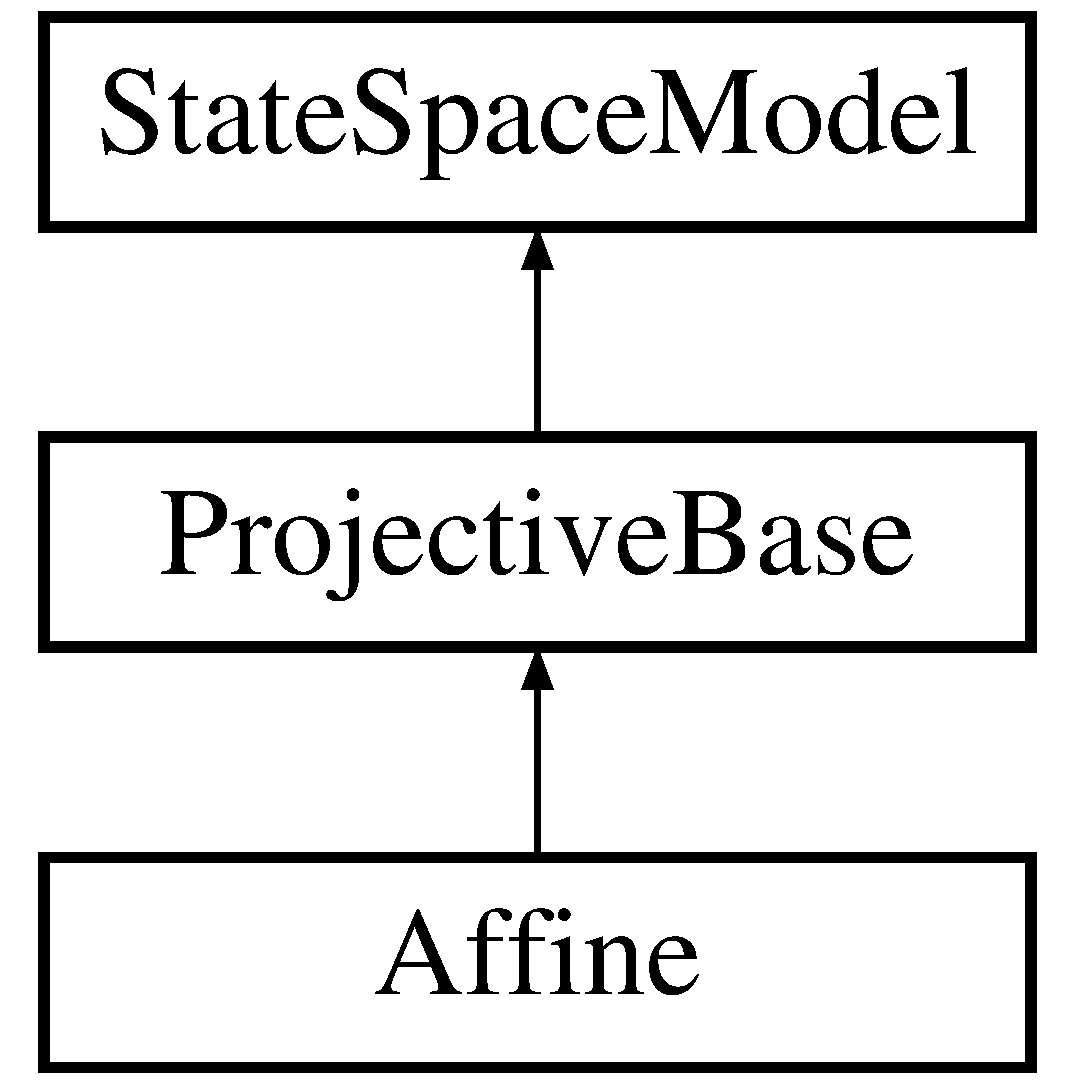
\includegraphics[height=3.000000cm]{classAffine}
\end{center}
\end{figure}
\subsection*{Public Types}
\begin{DoxyCompactItemize}
\item 
\hypertarget{classAffine_a1508564783c199efb28ec63911b1b1bf}{typedef \hyperlink{structAffineParams}{Affine\-Params} {\bfseries Param\-Type}}\label{classAffine_a1508564783c199efb28ec63911b1b1bf}

\end{DoxyCompactItemize}
\subsection*{Public Member Functions}
\begin{DoxyCompactItemize}
\item 
\hypertarget{classAffine_abe0773e87192293f2a3f003688fb9b58}{{\bfseries Affine} (const \hyperlink{structAffineParams}{Param\-Type} $\ast$params\-\_\-in=nullptr)}\label{classAffine_abe0773e87192293f2a3f003688fb9b58}

\item 
\hypertarget{classAffine_a715bc448785efa2d64904d737e07f7e4}{void {\bfseries set\-Corners} (const Corners\-T \&corners) override}\label{classAffine_a715bc448785efa2d64904d737e07f7e4}

\item 
\hypertarget{classAffine_a7640196abd86b4fa4b0c7a915ff65f0c}{void {\bfseries get\-Init\-Pix\-Grad} (Matrix2\-Xd \&ssm\-\_\-grad, int pix\-\_\-id) override}\label{classAffine_a7640196abd86b4fa4b0c7a915ff65f0c}

\item 
\hypertarget{classAffine_add3d8a33edf80035be84fdc70df4bf45}{void {\bfseries get\-Curr\-Pix\-Grad} (Matrix2\-Xd \&ssm\-\_\-grad, int pix\-\_\-id) override}\label{classAffine_add3d8a33edf80035be84fdc70df4bf45}

\item 
void \hyperlink{classAffine_a64387caa4e95c06167fc2d6afa453110}{cmpt\-Init\-Pix\-Jacobian} (Matrix\-Xd \&jacobian\-\_\-prod, const Pix\-Grad\-T \&am\-\_\-jacobian) override
\begin{DoxyCompactList}\small\item\em right multiplies the initial or current ssm jacobian with the provided am jacobian; though this can be accomplished by the search method itself with simple matrix multiplication, the ssm jacobian often satisfies several constraints (e.\-g. \end{DoxyCompactList}\item 
\hypertarget{classAffine_af92cc0960d824ee69279895cf6f16ec3}{void {\bfseries cmpt\-Pix\-Jacobian} (Matrix\-Xd \&jacobian\-\_\-prod, const Pix\-Grad\-T \&am\-\_\-jacobian) override}\label{classAffine_af92cc0960d824ee69279895cf6f16ec3}

\item 
\hypertarget{classAffine_a11de7d87156cb4ebb414f1859bda3e70}{void {\bfseries cmpt\-Approx\-Pix\-Jacobian} (Matrix\-Xd \&jacobian\-\_\-prod, const Pix\-Grad\-T \&pix\-\_\-jacobian) override}\label{classAffine_a11de7d87156cb4ebb414f1859bda3e70}

\item 
\hypertarget{classAffine_a0250ee9810c77fd9d8be873290512c67}{void {\bfseries cmpt\-Warped\-Pix\-Jacobian} (Matrix\-Xd \&jacobian\-\_\-prod, const Pix\-Grad\-T \&pix\-\_\-jacobian) override}\label{classAffine_a0250ee9810c77fd9d8be873290512c67}

\item 
\hypertarget{classAffine_a8e7721884e32d979034ae971103605a6}{void {\bfseries cmpt\-Init\-Pix\-Hessian} (Matrix\-Xd \&pix\-\_\-hess\-\_\-ssm, const Pix\-Hess\-T \&pix\-\_\-hess\-\_\-coord, const Pix\-Grad\-T \&pix\-\_\-grad) override}\label{classAffine_a8e7721884e32d979034ae971103605a6}

\item 
\hypertarget{classAffine_aaa0914ba34479e043c21a7e1e8546fa4}{void {\bfseries cmpt\-Pix\-Hessian} (Matrix\-Xd \&pix\-\_\-hess\-\_\-ssm, const Pix\-Hess\-T \&pix\-\_\-hess\-\_\-coord, const Pix\-Grad\-T \&pix\-\_\-grad) override}\label{classAffine_aaa0914ba34479e043c21a7e1e8546fa4}

\item 
\hypertarget{classAffine_a1e07504716b5d116642e03cf8f63bbfd}{void {\bfseries cmpt\-Warped\-Pix\-Hessian} (Matrix\-Xd \&\-\_\-d2\-I\-\_\-dp2, const Pix\-Hess\-T \&\-\_\-d2\-I\-\_\-dw2, const Pix\-Grad\-T \&d\-I\-\_\-dw) override}\label{classAffine_a1e07504716b5d116642e03cf8f63bbfd}

\item 
\hypertarget{classAffine_a00875afed231c96bd0833381cd72c85c}{void {\bfseries compositional\-Update} (const Vector\-Xd \&state\-\_\-update) override}\label{classAffine_a00875afed231c96bd0833381cd72c85c}

\item 
\hypertarget{classAffine_aad1af65ac5dda80f4e29ea780be90c3a}{void {\bfseries estimate\-Warp\-From\-Corners} (Vector\-Xd \&state\-\_\-update, const Corners\-T \&in\-\_\-corners, const Corners\-T \&out\-\_\-corners) override}\label{classAffine_aad1af65ac5dda80f4e29ea780be90c3a}

\item 
\hypertarget{classAffine_a3c6142bde028148e1617e23cdcf48904}{void {\bfseries estimate\-Warp\-From\-Pts} (Vector\-Xd \&state\-\_\-update, vector$<$ uchar $>$ \&mask, const vector$<$ cv\-::\-Point2f $>$ \&in\-\_\-pts, const vector$<$ cv\-::\-Point2f $>$ \&out\-\_\-pts, const \hyperlink{structSSMEstimatorParams}{Estimator\-Params} \&est\-\_\-params) override}\label{classAffine_a3c6142bde028148e1617e23cdcf48904}

\item 
\hypertarget{classAffine_abf133012708202550e4aa16161ce93a5}{void {\bfseries invert\-State} (Vector\-Xd \&inv\-\_\-state, const Vector\-Xd \&state) override}\label{classAffine_abf133012708202550e4aa16161ce93a5}

\item 
\hypertarget{classAffine_a1930e8a44e6541bef0f14f11ba535ee4}{void {\bfseries update\-Grad\-Pts} (double grad\-\_\-eps) override}\label{classAffine_a1930e8a44e6541bef0f14f11ba535ee4}

\item 
\hypertarget{classAffine_ae4cca8d0810e7d6c328a64df011c7b52}{void {\bfseries update\-Hess\-Pts} (double hess\-\_\-eps) override}\label{classAffine_ae4cca8d0810e7d6c328a64df011c7b52}

\item 
\hypertarget{classAffine_af1c117db413f5dc5896b9dfe137d5eda}{void {\bfseries set\-State} (const Vector\-Xd \&ssm\-\_\-state) override}\label{classAffine_af1c117db413f5dc5896b9dfe137d5eda}

\item 
\hypertarget{classAffine_ac1dea6ab2e5acfcc50c5fc1ea4a99c12}{void {\bfseries apply\-Warp\-To\-Corners} (Corners\-T \&warped\-\_\-corners, const Corners\-T \&orig\-\_\-corners, const Vector\-Xd \&state\-\_\-update) override}\label{classAffine_ac1dea6ab2e5acfcc50c5fc1ea4a99c12}

\item 
\hypertarget{classAffine_a1012a305b4a5f99447ea6bb7943377b9}{void {\bfseries apply\-Warp\-To\-Pts} (Matrix2\-Xd \&warped\-\_\-pts, const Matrix2\-Xd \&orig\-\_\-pts, const Vector\-Xd \&state\-\_\-update) override}\label{classAffine_a1012a305b4a5f99447ea6bb7943377b9}

\item 
\hypertarget{classAffine_af05041f4ee272cfcbec298f2b1d51b07}{void {\bfseries get\-Warp\-From\-State} (Matrix3d \&warp\-\_\-mat, const Vector\-Xd \&ssm\-\_\-state) override}\label{classAffine_af05041f4ee272cfcbec298f2b1d51b07}

\item 
\hypertarget{classAffine_aeb9e78b2f013ffa81bee8f928a97457f}{void {\bfseries get\-State\-From\-Warp} (Vector\-Xd \&state\-\_\-vec, const Matrix3d \&warp\-\_\-mat) override}\label{classAffine_aeb9e78b2f013ffa81bee8f928a97457f}

\item 
\hypertarget{classAffine_ad7e68a462deb51a5e0505c52c9c6fa52}{void {\bfseries generate\-Perturbation} (Vector\-Xd \&perturbation) override}\label{classAffine_ad7e68a462deb51a5e0505c52c9c6fa52}

\item 
\hypertarget{classAffine_a7bb7dc4edd20137486cf827d271bdca8}{void {\bfseries compositional\-Random\-Walk} (Vector\-Xd \&perturbed\-\_\-state, const Vector\-Xd \&base\-\_\-state) override}\label{classAffine_a7bb7dc4edd20137486cf827d271bdca8}

\item 
\hypertarget{classAffine_afabebe898c9bf0cab5caab714c6f3b79}{void {\bfseries additive\-Random\-Walk} (Vector\-Xd \&perturbed\-\_\-state, const Vector\-Xd \&base\-\_\-state) override}\label{classAffine_afabebe898c9bf0cab5caab714c6f3b79}

\item 
\hypertarget{classAffine_aab7fa4e999bae0e888c106dafe8db3d9}{void {\bfseries additive\-Auto\-Regression1} (Vector\-Xd \&perturbed\-\_\-state, Vector\-Xd \&perturbed\-\_\-ar, const Vector\-Xd \&base\-\_\-state, const Vector\-Xd \&base\-\_\-ar, double a=0.\-5) override}\label{classAffine_aab7fa4e999bae0e888c106dafe8db3d9}

\item 
\hypertarget{classAffine_a380a38a137d2fe0b80f7ede3b19048e8}{bool {\bfseries supports\-S\-P\-I} () override}\label{classAffine_a380a38a137d2fe0b80f7ede3b19048e8}

\end{DoxyCompactItemize}
\subsection*{Public Attributes}
\begin{DoxyCompactItemize}
\item 
\hypertarget{classAffine_a41caf13a6b620c5e22dcba8deb63650b}{\hyperlink{structAffineParams}{Param\-Type} {\bfseries params}}\label{classAffine_a41caf13a6b620c5e22dcba8deb63650b}

\end{DoxyCompactItemize}
\subsection*{Protected Member Functions}
\begin{DoxyCompactItemize}
\item 
\hypertarget{classAffine_a95f484115ee487b6e53e829a4e5c2842}{Vector6d {\bfseries state\-To\-Geom} (const Vector6d \&state)}\label{classAffine_a95f484115ee487b6e53e829a4e5c2842}

\item 
\hypertarget{classAffine_a4cbcce9fc44fcfbe7d3d8bae35c64e00}{Vector6d {\bfseries geom\-To\-State} (const Vector6d \&geom)}\label{classAffine_a4cbcce9fc44fcfbe7d3d8bae35c64e00}

\end{DoxyCompactItemize}
\subsection*{Protected Attributes}
\begin{DoxyCompactItemize}
\item 
\hypertarget{classAffine_aba7db43cadd85495352fcc734f80ac78}{Matrix23d {\bfseries rand\-\_\-d}}\label{classAffine_aba7db43cadd85495352fcc734f80ac78}

\item 
\hypertarget{classAffine_ac74620a4e7737b02da98524be1e58aa7}{Vector2d {\bfseries rand\-\_\-t}}\label{classAffine_ac74620a4e7737b02da98524be1e58aa7}

\item 
\hypertarget{classAffine_a80745c0bb5b20063a879a84f42004bc9}{Matrix23d {\bfseries init\-\_\-canonical\-\_\-pts}}\label{classAffine_a80745c0bb5b20063a879a84f42004bc9}

\item 
\hypertarget{classAffine_a62706295414c41823c97635c24de71f3}{Matrix23d {\bfseries perturbed\-\_\-canonical\-\_\-pts}}\label{classAffine_a62706295414c41823c97635c24de71f3}

\end{DoxyCompactItemize}


\subsection{Member Function Documentation}
\hypertarget{classAffine_a64387caa4e95c06167fc2d6afa453110}{\index{Affine@{Affine}!cmpt\-Init\-Pix\-Jacobian@{cmpt\-Init\-Pix\-Jacobian}}
\index{cmpt\-Init\-Pix\-Jacobian@{cmpt\-Init\-Pix\-Jacobian}!Affine@{Affine}}
\subsubsection[{cmpt\-Init\-Pix\-Jacobian}]{\setlength{\rightskip}{0pt plus 5cm}void Affine\-::cmpt\-Init\-Pix\-Jacobian (
\begin{DoxyParamCaption}
\item[{Matrix\-Xd \&}]{jacobian\-\_\-prod, }
\item[{const Pix\-Grad\-T \&}]{pixel\-\_\-grad}
\end{DoxyParamCaption}
)\hspace{0.3cm}{\ttfamily [override]}, {\ttfamily [virtual]}}}\label{classAffine_a64387caa4e95c06167fc2d6afa453110}


right multiplies the initial or current ssm jacobian with the provided am jacobian; though this can be accomplished by the search method itself with simple matrix multiplication, the ssm jacobian often satisfies several constraints (e.\-g. 

sparsity) that can be exploited to gain computational savings by manually computing the product matrix 

Reimplemented from \hyperlink{classStateSpaceModel_ac956c679581e746891c62755fe715b3b}{State\-Space\-Model}.



The documentation for this class was generated from the following file\-:\begin{DoxyCompactItemize}
\item 
S\-S\-M/include/mtf/\-S\-S\-M/Affine.\-h\end{DoxyCompactItemize}

\hypertarget{classAffineEstimator}{\section{Affine\-Estimator Class Reference}
\label{classAffineEstimator}\index{Affine\-Estimator@{Affine\-Estimator}}
}
Inheritance diagram for Affine\-Estimator\-:\begin{figure}[H]
\begin{center}
\leavevmode
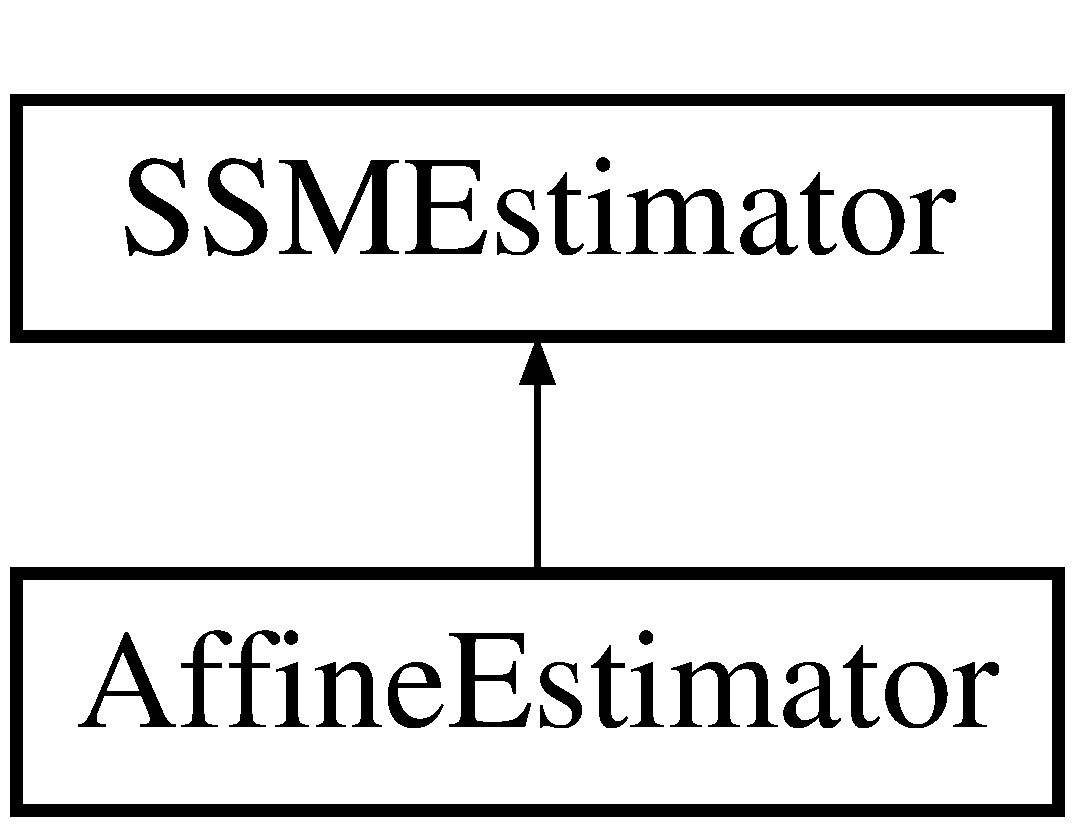
\includegraphics[height=2.000000cm]{classAffineEstimator}
\end{center}
\end{figure}
\subsection*{Public Member Functions}
\begin{DoxyCompactItemize}
\item 
\hypertarget{classAffineEstimator_ac19ac61c0ef244dcbdb6b33a61228389}{{\bfseries Affine\-Estimator} (int model\-Points)}\label{classAffineEstimator_ac19ac61c0ef244dcbdb6b33a61228389}

\item 
\hypertarget{classAffineEstimator_aebc1eec833f3c3cfb64191761aee8144}{int {\bfseries run\-Kernel} (const Cv\-Mat $\ast$m1, const Cv\-Mat $\ast$m2, Cv\-Mat $\ast$model) override}\label{classAffineEstimator_aebc1eec833f3c3cfb64191761aee8144}

\item 
\hypertarget{classAffineEstimator_a94e88dde72d03a9f5fd10ea9858e1869}{bool {\bfseries refine} (const Cv\-Mat $\ast$m1, const Cv\-Mat $\ast$m2, Cv\-Mat $\ast$model, int max\-Iters) override}\label{classAffineEstimator_a94e88dde72d03a9f5fd10ea9858e1869}

\end{DoxyCompactItemize}
\subsection*{Protected Member Functions}
\begin{DoxyCompactItemize}
\item 
\hypertarget{classAffineEstimator_a796eb2c1999a2fb599989fcfee5a455d}{void {\bfseries compute\-Reproj\-Error} (const Cv\-Mat $\ast$m1, const Cv\-Mat $\ast$m2, const Cv\-Mat $\ast$model, Cv\-Mat $\ast$error) override}\label{classAffineEstimator_a796eb2c1999a2fb599989fcfee5a455d}

\end{DoxyCompactItemize}
\subsection*{Additional Inherited Members}


The documentation for this class was generated from the following file\-:\begin{DoxyCompactItemize}
\item 
S\-S\-M/include/mtf/\-S\-S\-M/S\-S\-M\-Estimator.\-h\end{DoxyCompactItemize}

\hypertarget{structAffineParams}{\section{Affine\-Params Struct Reference}
\label{structAffineParams}\index{Affine\-Params@{Affine\-Params}}
}
Inheritance diagram for Affine\-Params\-:\begin{figure}[H]
\begin{center}
\leavevmode
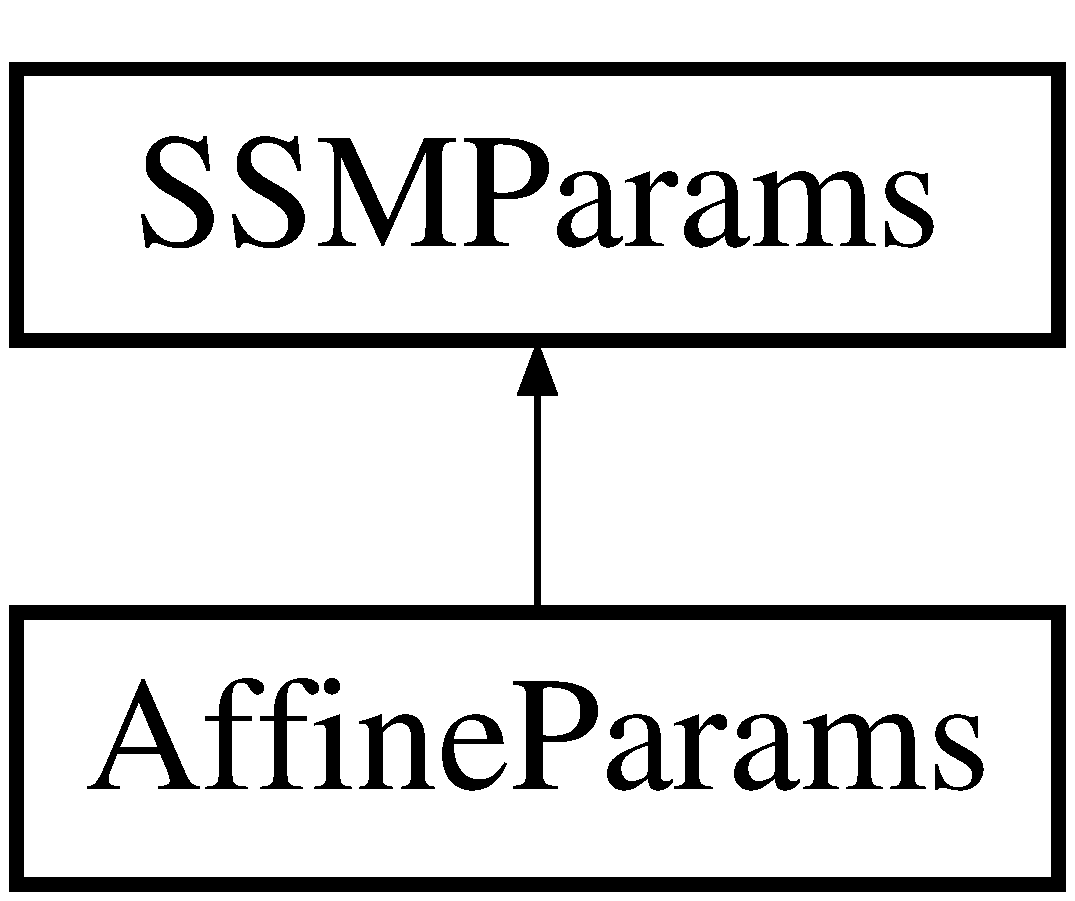
\includegraphics[height=2.000000cm]{structAffineParams}
\end{center}
\end{figure}
\subsection*{Public Member Functions}
\begin{DoxyCompactItemize}
\item 
\hypertarget{structAffineParams_a17bcd5f9b67039b290e21a50b9a62947}{{\bfseries Affine\-Params} (const \hyperlink{structSSMParams}{S\-S\-M\-Params} $\ast$ssm\-\_\-params, bool \-\_\-normalized\-\_\-init, bool \-\_\-pt\-\_\-based\-\_\-sampling, bool \-\_\-debug\-\_\-mode)}\label{structAffineParams_a17bcd5f9b67039b290e21a50b9a62947}

\item 
\hypertarget{structAffineParams_ae0985577e304c177588007ac80e6c353}{{\bfseries Affine\-Params} (const \hyperlink{structAffineParams}{Affine\-Params} $\ast$params=nullptr)}\label{structAffineParams_ae0985577e304c177588007ac80e6c353}

\end{DoxyCompactItemize}
\subsection*{Public Attributes}
\begin{DoxyCompactItemize}
\item 
\hypertarget{structAffineParams_ab4c42aa3f2270811a6d3663ba445e9c9}{bool {\bfseries normalized\-\_\-init}}\label{structAffineParams_ab4c42aa3f2270811a6d3663ba445e9c9}

\item 
\hypertarget{structAffineParams_ab2c63e280584f9e50666b0b18865f78b}{bool {\bfseries pt\-\_\-based\-\_\-sampling}}\label{structAffineParams_ab2c63e280584f9e50666b0b18865f78b}

\item 
\hypertarget{structAffineParams_a580684e98999b8a2fee6de66290abb1a}{bool {\bfseries debug\-\_\-mode}}\label{structAffineParams_a580684e98999b8a2fee6de66290abb1a}

\end{DoxyCompactItemize}


The documentation for this struct was generated from the following file\-:\begin{DoxyCompactItemize}
\item 
S\-S\-M/include/mtf/\-S\-S\-M/Affine.\-h\end{DoxyCompactItemize}

\hypertarget{structAMParams}{\section{A\-M\-Params Struct Reference}
\label{structAMParams}\index{A\-M\-Params@{A\-M\-Params}}
}
Inheritance diagram for A\-M\-Params\-:\begin{figure}[H]
\begin{center}
\leavevmode
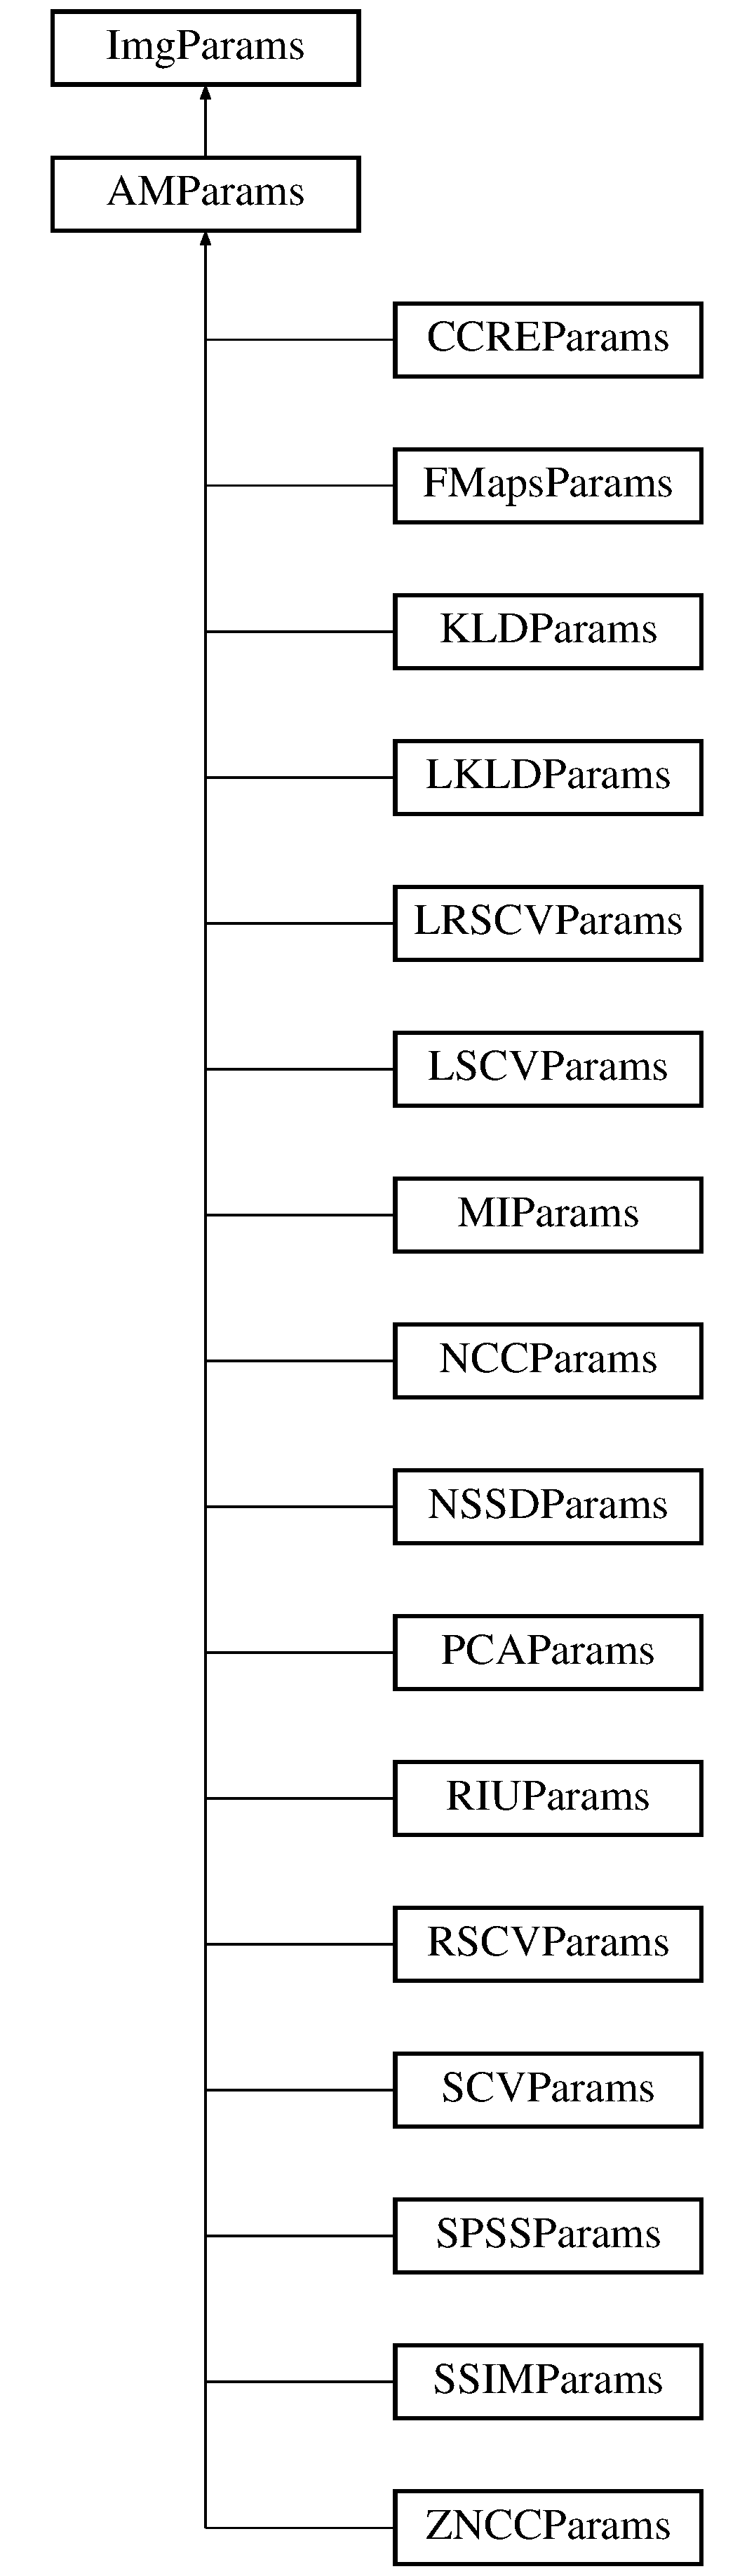
\includegraphics[height=12.000000cm]{structAMParams}
\end{center}
\end{figure}
\subsection*{Public Member Functions}
\begin{DoxyCompactItemize}
\item 
\hypertarget{structAMParams_a750182dcee7d777bc63cad82154f7ff9}{{\bfseries A\-M\-Params} (int \-\_\-resx, int \-\_\-resy, double \-\_\-grad\-\_\-eps=G\-R\-A\-D\-\_\-\-E\-P\-S, double \-\_\-hess\-\_\-eps=H\-E\-S\-S\-\_\-\-E\-P\-S, \hyperlink{classIlluminationModel}{Illumination\-Model} $\ast$\-\_\-ilm=nullptr)}\label{structAMParams_a750182dcee7d777bc63cad82154f7ff9}

\item 
\hypertarget{structAMParams_acea86047c12b02c939ac428722c33361}{{\bfseries A\-M\-Params} (const \hyperlink{structAMParams}{A\-M\-Params} $\ast$am\-\_\-params=nullptr)}\label{structAMParams_acea86047c12b02c939ac428722c33361}

\end{DoxyCompactItemize}
\subsection*{Public Attributes}
\begin{DoxyCompactItemize}
\item 
\hypertarget{structAMParams_a6e8a27a6b3241a763c6b198b63bef730}{\hyperlink{classIlluminationModel}{Illumination\-Model} $\ast$ \hyperlink{structAMParams_a6e8a27a6b3241a763c6b198b63bef730}{ilm}}\label{structAMParams_a6e8a27a6b3241a763c6b198b63bef730}

\begin{DoxyCompactList}\small\item\em optional parametric function of pixel values that can account for lighting changes \end{DoxyCompactList}\end{DoxyCompactItemize}


The documentation for this struct was generated from the following file\-:\begin{DoxyCompactItemize}
\item 
A\-M/include/mtf/\-A\-M/Appearance\-Model.\-h\end{DoxyCompactItemize}

\hypertarget{structAMStatus}{\section{A\-M\-Status Struct Reference}
\label{structAMStatus}\index{A\-M\-Status@{A\-M\-Status}}
}


set of indicator variables to keep track of which dependent state variables need updating and executing the update expression for any variable only when at least one of the other variables it depends on has been updated; this can help to increase speed by avoiding repeated computations  




{\ttfamily \#include $<$Appearance\-Model.\-h$>$}

Inheritance diagram for A\-M\-Status\-:\begin{figure}[H]
\begin{center}
\leavevmode
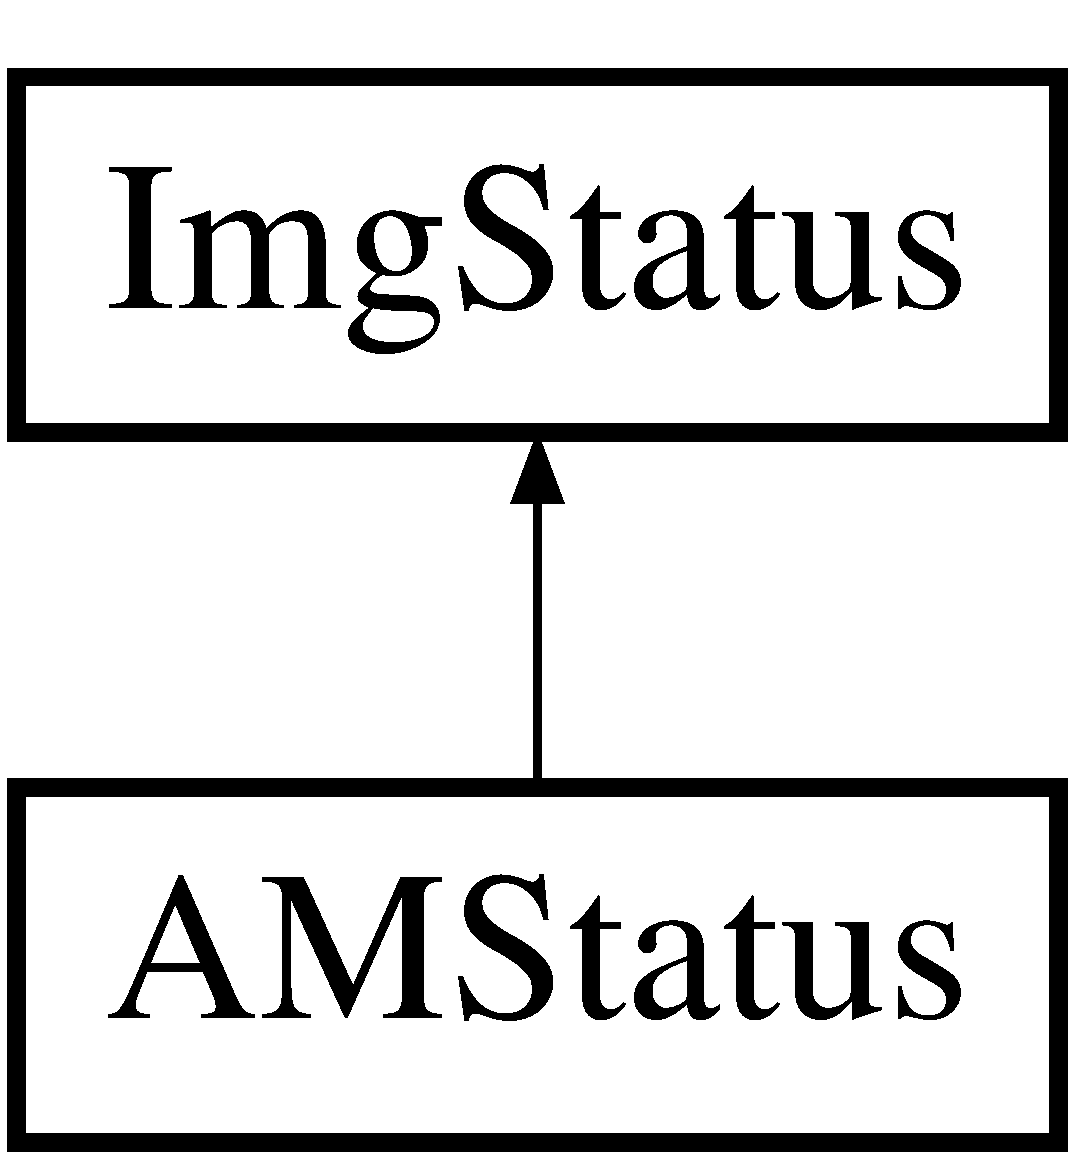
\includegraphics[height=2.000000cm]{structAMStatus}
\end{center}
\end{figure}
\subsection*{Public Member Functions}
\begin{DoxyCompactItemize}
\item 
\hypertarget{structAMStatus_a58c0fe7c4625f1dc26701e65d2b7d6dc}{void {\bfseries set} ()}\label{structAMStatus_a58c0fe7c4625f1dc26701e65d2b7d6dc}

\item 
\hypertarget{structAMStatus_a59dbffa885af1ad239578eaf417c0eee}{void {\bfseries clear} ()}\label{structAMStatus_a59dbffa885af1ad239578eaf417c0eee}

\end{DoxyCompactItemize}
\subsection*{Public Attributes}
\begin{DoxyCompactItemize}
\item 
\hypertarget{structAMStatus_a31496e83632ea2df36b2236aae6936d6}{bool {\bfseries similarity}}\label{structAMStatus_a31496e83632ea2df36b2236aae6936d6}

\item 
\hypertarget{structAMStatus_a52366a59d56c772d8c12e1cbd6a40ae5}{bool {\bfseries grad}}\label{structAMStatus_a52366a59d56c772d8c12e1cbd6a40ae5}

\item 
\hypertarget{structAMStatus_ae4f44ba5f170022bacdec857f4d450e8}{bool {\bfseries hess}}\label{structAMStatus_ae4f44ba5f170022bacdec857f4d450e8}

\item 
\hypertarget{structAMStatus_a39fb50fa4fd243622b17956761da42d8}{bool {\bfseries sampler}}\label{structAMStatus_a39fb50fa4fd243622b17956761da42d8}

\end{DoxyCompactItemize}


\subsection{Detailed Description}
set of indicator variables to keep track of which dependent state variables need updating and executing the update expression for any variable only when at least one of the other variables it depends on has been updated; this can help to increase speed by avoiding repeated computations 

The documentation for this struct was generated from the following file\-:\begin{DoxyCompactItemize}
\item 
A\-M/include/mtf/\-A\-M/Appearance\-Model.\-h\end{DoxyCompactItemize}

\hypertarget{classAppearanceModel}{\section{Appearance\-Model Class Reference}
\label{classAppearanceModel}\index{Appearance\-Model@{Appearance\-Model}}
}


Similarity function that indicates how well a candidate warped patch matches the template.  




{\ttfamily \#include $<$Appearance\-Model.\-h$>$}

Inheritance diagram for Appearance\-Model\-:\begin{figure}[H]
\begin{center}
\leavevmode
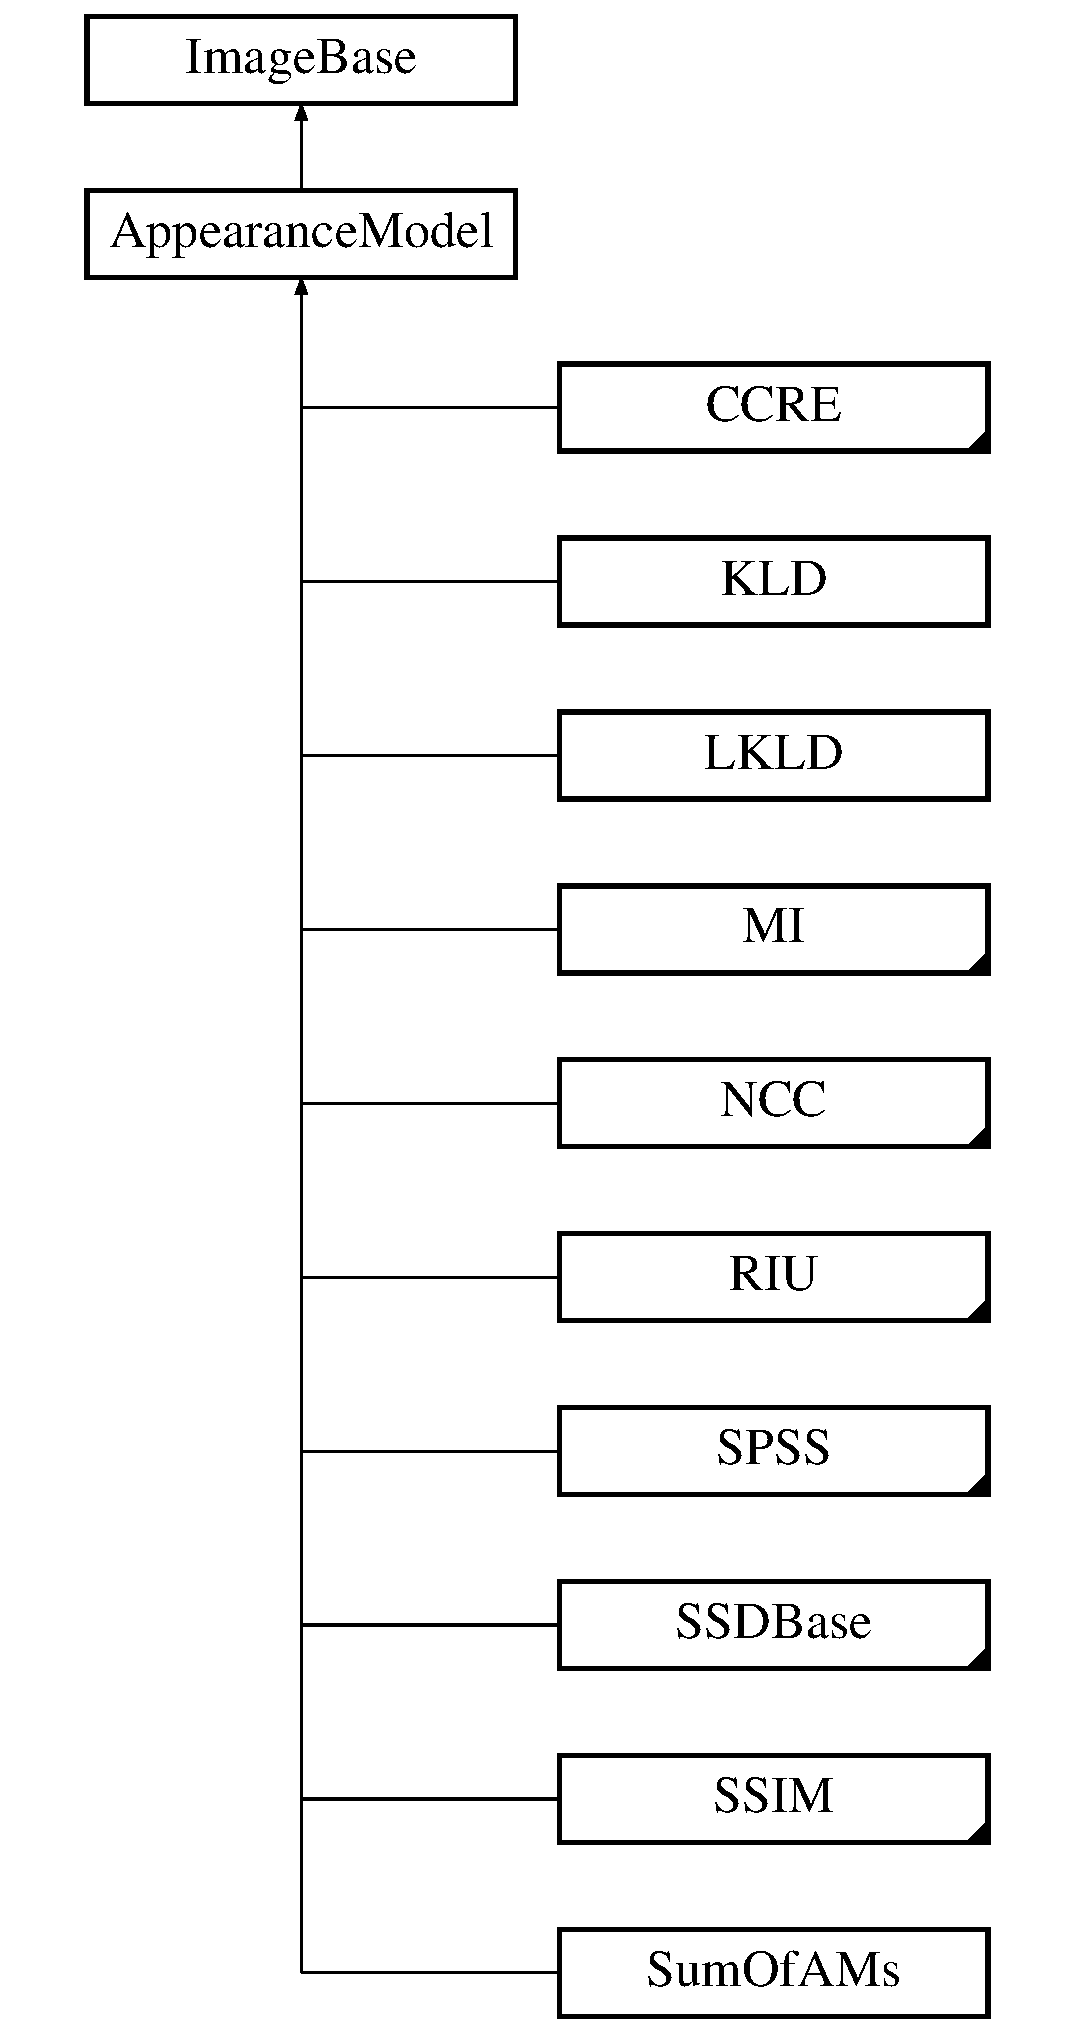
\includegraphics[height=12.000000cm]{classAppearanceModel}
\end{center}
\end{figure}
\subsection*{Public Types}
\begin{DoxyCompactItemize}
\item 
\hypertarget{classAppearanceModel_a6e19328a81eb4c05ce1ad2e2887e17a3}{typedef double {\bfseries Element\-Type}}\label{classAppearanceModel_a6e19328a81eb4c05ce1ad2e2887e17a3}

\item 
\hypertarget{classAppearanceModel_af0cc383d55025c98be4de620d448cb20}{typedef double {\bfseries Result\-Type}}\label{classAppearanceModel_af0cc383d55025c98be4de620d448cb20}

\end{DoxyCompactItemize}
\subsection*{Public Member Functions}
\begin{DoxyCompactItemize}
\item 
\hypertarget{classAppearanceModel_a0b0eeb5779fa227bffd356c9562fc583}{\hyperlink{classAppearanceModel_a0b0eeb5779fa227bffd356c9562fc583}{Appearance\-Model} (const \hyperlink{structAMParams}{A\-M\-Params} $\ast$params=nullptr, const int \-\_\-n\-\_\-channels=1)}\label{classAppearanceModel_a0b0eeb5779fa227bffd356c9562fc583}

\begin{DoxyCompactList}\small\item\em default and value constructor \end{DoxyCompactList}\item 
\hypertarget{classAppearanceModel_a457d2fefd61966035659a8212da93017}{virtual \hyperlink{classAppearanceModel_a457d2fefd61966035659a8212da93017}{$\sim$\-Appearance\-Model} ()}\label{classAppearanceModel_a457d2fefd61966035659a8212da93017}

\begin{DoxyCompactList}\small\item\em destructor \end{DoxyCompactList}\item 
\hypertarget{classAppearanceModel_af1c127fe00057b7674502885071c586d}{virtual int \hyperlink{classAppearanceModel_af1c127fe00057b7674502885071c586d}{get\-State\-Size} () const }\label{classAppearanceModel_af1c127fe00057b7674502885071c586d}

\begin{DoxyCompactList}\small\item\em accessor methods \end{DoxyCompactList}\item 
\hypertarget{classAppearanceModel_abf2f3cd69c2ac981c842b7ae0fe2fbef}{virtual double {\bfseries get\-Similarity} () const }\label{classAppearanceModel_abf2f3cd69c2ac981c842b7ae0fe2fbef}

\item 
\hypertarget{classAppearanceModel_a2486d4c5b7aeccf7b1b41c29f7a27099}{virtual double \hyperlink{classAppearanceModel_a2486d4c5b7aeccf7b1b41c29f7a27099}{get\-Likelihood} () const }\label{classAppearanceModel_a2486d4c5b7aeccf7b1b41c29f7a27099}

\begin{DoxyCompactList}\small\item\em returns a normalized version of the similarity that lies between 0 and 1 and can be interpreted as the likelihood that the current patch represents the same object as the initial patch \end{DoxyCompactList}\item 
\hypertarget{classAppearanceModel_a118172fa91ad6a85b2bfb22cb97ce8f8}{virtual const Vector\-Xd \& {\bfseries get\-State} ()}\label{classAppearanceModel_a118172fa91ad6a85b2bfb22cb97ce8f8}

\item 
\hypertarget{classAppearanceModel_afed0a650b7c50607781aab7a1efad295}{virtual const Row\-Vector\-Xd \& {\bfseries get\-Init\-Grad} () const }\label{classAppearanceModel_afed0a650b7c50607781aab7a1efad295}

\item 
\hypertarget{classAppearanceModel_a3a368798dc03a8ad0ebd4beaa0679776}{virtual const Row\-Vector\-Xd \& {\bfseries get\-Curr\-Grad} () const }\label{classAppearanceModel_a3a368798dc03a8ad0ebd4beaa0679776}

\item 
\hypertarget{classAppearanceModel_a615e1e41bfe54f3c36d9ea88d2a3da57}{virtual void \hyperlink{classAppearanceModel_a615e1e41bfe54f3c36d9ea88d2a3da57}{set\-Similarity} (double \-\_\-similarity)}\label{classAppearanceModel_a615e1e41bfe54f3c36d9ea88d2a3da57}

\begin{DoxyCompactList}\small\item\em modifier methods \end{DoxyCompactList}\item 
\hypertarget{classAppearanceModel_aff31a111da5b55e52012c0d23360e7c3}{virtual void {\bfseries set\-Init\-Grad} (const Row\-Vector\-Xd \&df\-\_\-d\-I)}\label{classAppearanceModel_aff31a111da5b55e52012c0d23360e7c3}

\item 
\hypertarget{classAppearanceModel_aa908daa1a4fc6e6a2300d472f27fa256}{virtual void {\bfseries set\-Curr\-Grad} (const Row\-Vector\-Xd \&df\-\_\-d\-I)}\label{classAppearanceModel_aa908daa1a4fc6e6a2300d472f27fa256}

\item 
virtual void \hyperlink{classAppearanceModel_abcd79170a5fccc0e9aa10675404ad655}{initialize\-Similarity} ()
\begin{DoxyCompactList}\small\item\em methods to initialize the state variables -\/ to be called once when the tracker is initialized. \end{DoxyCompactList}\item 
\hypertarget{classAppearanceModel_a553b254253ba3c10672b401ff2dbb403}{virtual void {\bfseries initialize\-Grad} ()}\label{classAppearanceModel_a553b254253ba3c10672b401ff2dbb403}

\item 
virtual void \hyperlink{classAppearanceModel_afb47df1d5e8a74f41ac70af3612180d2}{initialize\-Hess} ()
\begin{DoxyCompactList}\small\item\em even though the Hessian of the error norm w.\-r.\-t. \end{DoxyCompactList}\item 
virtual void \hyperlink{classAppearanceModel_a06136ecd903e85ed2007da2c7b12bd58}{update\-Similarity} (bool prereq\-\_\-only=true)
\begin{DoxyCompactList}\small\item\em functions for updating state variables when a new image arrives \end{DoxyCompactList}\item 
\hypertarget{classAppearanceModel_a184dafcec26de15236550a9011fb93f9}{virtual void {\bfseries update\-State} (const Vector\-Xd \&state\-\_\-update)}\label{classAppearanceModel_a184dafcec26de15236550a9011fb93f9}

\item 
\hypertarget{classAppearanceModel_a5442374c0c95d4649cf1f9234f23e422}{virtual void {\bfseries invert\-State} (Vector\-Xd \&inv\-\_\-p, const Vector\-Xd \&p)}\label{classAppearanceModel_a5442374c0c95d4649cf1f9234f23e422}

\item 
\hypertarget{classAppearanceModel_a5ad5890e5978a0025300acacddb0d97f}{virtual void {\bfseries update\-Init\-Grad} ()}\label{classAppearanceModel_a5ad5890e5978a0025300acacddb0d97f}

\item 
\hypertarget{classAppearanceModel_ae5e2601d32475be3001b77b02108845b}{virtual void {\bfseries update\-Curr\-Grad} ()}\label{classAppearanceModel_ae5e2601d32475be3001b77b02108845b}

\item 
\hypertarget{classAppearanceModel_a292b85c011140c14e81dd8f1a30933d6}{virtual void {\bfseries update\-Param\-Grad} ()}\label{classAppearanceModel_a292b85c011140c14e81dd8f1a30933d6}

\item 
virtual void \hyperlink{classAppearanceModel_a8f3a4e961bc1a5c9acd64bf3b376f859}{cmpt\-Init\-Jacobian} (Row\-Vector\-Xd \&df\-\_\-dp, const Matrix\-Xd \&d\-I0\-\_\-dpssm)
\begin{DoxyCompactList}\small\item\em ----- interfacing functions that take pixel jacobians/\-Hessians w.\-r.\-t. \end{DoxyCompactList}\item 
\hypertarget{classAppearanceModel_a2ab29cd5820e12cb0b01f1bf99210b8d}{virtual void {\bfseries cmpt\-Curr\-Jacobian} (Row\-Vector\-Xd \&df\-\_\-dp, const Matrix\-Xd \&d\-It\-\_\-dpssm)}\label{classAppearanceModel_a2ab29cd5820e12cb0b01f1bf99210b8d}

\item 
virtual void \hyperlink{classAppearanceModel_a6fc5e1c4eeacc794f1783926c6613db3}{cmpt\-Difference\-Of\-Jacobians} (Row\-Vector\-Xd \&df\-\_\-dp\-\_\-diff, const Matrix\-Xd \&d\-I0\-\_\-dpssm, const Matrix\-Xd \&d\-It\-\_\-dpssm)
\begin{DoxyCompactList}\small\item\em multiplies the gradients of the current error norm w.\-r.\-t. \end{DoxyCompactList}\item 
virtual void \hyperlink{classAppearanceModel_ab153b47d09f121796d3f411626a5321c}{cmpt\-Init\-Hessian} (Matrix\-Xd \&d2f\-\_\-dp2, const Matrix\-Xd \&d\-I0\-\_\-dpssm)
\begin{DoxyCompactList}\small\item\em compute the S x S Hessian of the error norm using the supplied N x S Jacobian of pixel values w.\-r.\-t. \end{DoxyCompactList}\item 
\hypertarget{classAppearanceModel_a5052efc12c81f67dcfcaba5a197ed74e}{virtual void {\bfseries cmpt\-Curr\-Hessian} (Matrix\-Xd \&d2f\-\_\-dp2, const Matrix\-Xd \&d\-It\-\_\-dpssm)}\label{classAppearanceModel_a5052efc12c81f67dcfcaba5a197ed74e}

\item 
\hypertarget{classAppearanceModel_ad55ef54a7c21ff6ee7fb77aac4b33453}{virtual void {\bfseries cmpt\-Self\-Hessian} (Matrix\-Xd \&d2f\-\_\-dp2, const Matrix\-Xd \&d\-It\-\_\-dpssm)}\label{classAppearanceModel_ad55ef54a7c21ff6ee7fb77aac4b33453}

\item 
\hypertarget{classAppearanceModel_aa904369642a3ef3c8f0e49b46861166d}{virtual void \hyperlink{classAppearanceModel_aa904369642a3ef3c8f0e49b46861166d}{cmpt\-Init\-Hessian} (Matrix\-Xd \&d2f\-\_\-dp2, const Matrix\-Xd \&d\-I0\-\_\-dpssm, const Matrix\-Xd \&d2\-I0\-\_\-dpssm2)}\label{classAppearanceModel_aa904369642a3ef3c8f0e49b46861166d}

\begin{DoxyCompactList}\small\item\em compute the exact Hessian by considering the second order terms too \end{DoxyCompactList}\item 
\hypertarget{classAppearanceModel_a27207e73e39f5270bb8ef1193cb4f768}{virtual void {\bfseries cmpt\-Curr\-Hessian} (Matrix\-Xd \&d2f\-\_\-dp2, const Matrix\-Xd \&d\-It\-\_\-dpssm, const Matrix\-Xd \&d2\-It\-\_\-dpssm2)}\label{classAppearanceModel_a27207e73e39f5270bb8ef1193cb4f768}

\item 
\hypertarget{classAppearanceModel_a4d4f07a1240bb49de9d6113943fe7aa1}{virtual void {\bfseries cmpt\-Self\-Hessian} (Matrix\-Xd \&d2f\-\_\-dp2, const Matrix\-Xd \&d\-It\-\_\-dpssm, const Matrix\-Xd \&d2\-I\-\_\-dpssm2)}\label{classAppearanceModel_a4d4f07a1240bb49de9d6113943fe7aa1}

\item 
\hypertarget{classAppearanceModel_ad8171a2e748a9cbc22f3c7d7381c670b}{virtual void \hyperlink{classAppearanceModel_ad8171a2e748a9cbc22f3c7d7381c670b}{cmpt\-Sum\-Of\-Hessians} (Matrix\-Xd \&d2f\-\_\-dp2\-\_\-sum, const Matrix\-Xd \&d\-I0\-\_\-dpssm, const Matrix\-Xd \&d\-It\-\_\-dpssm)}\label{classAppearanceModel_ad8171a2e748a9cbc22f3c7d7381c670b}

\begin{DoxyCompactList}\small\item\em analogous to cmpt\-Difference\-Of\-Jacobians except for computing the mean of the current and initial Hessians \end{DoxyCompactList}\item 
\hypertarget{classAppearanceModel_afc5bac85b112cc975be844744ee8ccff}{virtual void {\bfseries cmpt\-Sum\-Of\-Hessians} (Matrix\-Xd \&d2f\-\_\-dp2\-\_\-sum, const Matrix\-Xd \&d\-I0\-\_\-dpssm, const Matrix\-Xd \&d\-It\-\_\-dpssm, const Matrix\-Xd \&d2\-I0\-\_\-dpssm2, const Matrix\-Xd \&d2\-It\-\_\-dpssm2)}\label{classAppearanceModel_afc5bac85b112cc975be844744ee8ccff}

\item 
\hypertarget{classAppearanceModel_a1db42141a7b09b554cd77ce4e7d7d25c}{virtual void {\bfseries set\-S\-P\-I\-Mask} (const bool $\ast$\-\_\-spi\-\_\-mask)}\label{classAppearanceModel_a1db42141a7b09b554cd77ce4e7d7d25c}

\item 
\hypertarget{classAppearanceModel_a45f6a5f859fb6418b848bc9c4478dbd3}{virtual const bool $\ast$ {\bfseries get\-S\-P\-I\-Mask} () const }\label{classAppearanceModel_a45f6a5f859fb6418b848bc9c4478dbd3}

\item 
\hypertarget{classAppearanceModel_ab368ad2693bb06b7e6b77b77afb92321}{virtual void {\bfseries clear\-S\-P\-I\-Mask} ()}\label{classAppearanceModel_ab368ad2693bb06b7e6b77b77afb92321}

\item 
\hypertarget{classAppearanceModel_a119b97402d3bb7041d921961e3722cf4}{virtual bool \hyperlink{classAppearanceModel_a119b97402d3bb7041d921961e3722cf4}{supports\-S\-P\-I} () const }\label{classAppearanceModel_a119b97402d3bb7041d921961e3722cf4}

\begin{DoxyCompactList}\small\item\em should be overridden by an implementing class once it implements S\-P\-I functionality for all functions where it makes logical sense \end{DoxyCompactList}\item 
\hypertarget{classAppearanceModel_a0cd5810a7ceca3418eaed254b4f11196}{virtual void \hyperlink{classAppearanceModel_a0cd5810a7ceca3418eaed254b4f11196}{set\-First\-Iter} ()}\label{classAppearanceModel_a0cd5810a7ceca3418eaed254b4f11196}

\begin{DoxyCompactList}\small\item\em should be called before performing the first iteration on a new image to indicate that the image has changed since the last time the update funcvtions were called \end{DoxyCompactList}\item 
\hypertarget{classAppearanceModel_a22302ac79fade071132848888ee050d1}{virtual void \hyperlink{classAppearanceModel_a22302ac79fade071132848888ee050d1}{clear\-First\-Iter} ()}\label{classAppearanceModel_a22302ac79fade071132848888ee050d1}

\begin{DoxyCompactList}\small\item\em should be called after the first iteration on a new frame is done \end{DoxyCompactList}\item 
\hypertarget{classAppearanceModel_adba6fa45d22db0134b365e1450a7b751}{\hyperlink{structImgStatus}{Img\-Status} $\ast$ {\bfseries is\-Initialized} () override}\label{classAppearanceModel_adba6fa45d22db0134b365e1450a7b751}

\item 
\hypertarget{classAppearanceModel_a3f8dd00e2abca94e123c2e44094de1dc}{virtual void {\bfseries set\-Init\-Status} ()}\label{classAppearanceModel_a3f8dd00e2abca94e123c2e44094de1dc}

\item 
\hypertarget{classAppearanceModel_a4809d14b7283044bbcb7361bca874070}{virtual void {\bfseries clear\-Init\-Status} ()}\label{classAppearanceModel_a4809d14b7283044bbcb7361bca874070}

\item 
virtual bool \hyperlink{classAppearanceModel_a432b2d068bf735abfa58c023773e1721}{is\-Symmetrical} () const 
\begin{DoxyCompactList}\small\item\em return false if the similarity function f is not symmetrical, i.\-e. \end{DoxyCompactList}\item 
\hypertarget{classAppearanceModel_a4e003afff892e69cf673e92710760563}{virtual double \hyperlink{classAppearanceModel_a4e003afff892e69cf673e92710760563}{operator()} (const double $\ast$a, const double $\ast$b, size\-\_\-t dist\-\_\-size, double worst\-\_\-dist=-\/1) const }\label{classAppearanceModel_a4e003afff892e69cf673e92710760563}

\begin{DoxyCompactList}\small\item\em computes the distance / dissimilarity between two patches where each is codified or represented by a suitable distance feature computed using update\-Dist\-Feat \end{DoxyCompactList}\item 
\hypertarget{classAppearanceModel_a04b3f66700a863ec171b12e8d016065b}{virtual void \hyperlink{classAppearanceModel_a04b3f66700a863ec171b12e8d016065b}{initialize\-Dist\-Feat} ()}\label{classAppearanceModel_a04b3f66700a863ec171b12e8d016065b}

\begin{DoxyCompactList}\small\item\em to be called once during initialization if any of the distance feature functionality is to be used \end{DoxyCompactList}\item 
virtual void \hyperlink{classAppearanceModel_afc815587980df0cd28412a2cd1670854}{update\-Dist\-Feat} ()
\begin{DoxyCompactList}\small\item\em computes a \char`\"{}distance\char`\"{} vector using the current image patch such that, when the distance vectors corresponding to two patches are passed to the distance operator above, it uses these to compute a scalar that measures the distance or dissimilarity between the two patches; this distance vector should be designed so as to offload as much computation as possible from the distance operator, i.\-e. \end{DoxyCompactList}\item 
\hypertarget{classAppearanceModel_a205dc9e522814207caab3f243acba87a}{virtual const double $\ast$ {\bfseries get\-Dist\-Feat} ()}\label{classAppearanceModel_a205dc9e522814207caab3f243acba87a}

\item 
\hypertarget{classAppearanceModel_aa01514bdfceaeaed207ac279c3f10afa}{virtual void \hyperlink{classAppearanceModel_aa01514bdfceaeaed207ac279c3f10afa}{update\-Dist\-Feat} (double $\ast$feat\-\_\-addr)}\label{classAppearanceModel_aa01514bdfceaeaed207ac279c3f10afa}

\begin{DoxyCompactList}\small\item\em overloaded version to write the distance feature directly to a row (or column) of a matrix storing the distance features corresponding to several patches; \end{DoxyCompactList}\item 
\hypertarget{classAppearanceModel_affa40a42a35edc8dd1d2d06344013315}{virtual int \hyperlink{classAppearanceModel_affa40a42a35edc8dd1d2d06344013315}{get\-Dist\-Feat\-Size} ()}\label{classAppearanceModel_affa40a42a35edc8dd1d2d06344013315}

\begin{DoxyCompactList}\small\item\em returns the size of the distance vector \end{DoxyCompactList}\item 
\hypertarget{classAppearanceModel_a8742b3a634db0cf593ab510bced23b3c}{virtual void {\bfseries initialize\-Sampler} (const Vector\-Xd \&state\-\_\-sigma, const Vector\-Xd \&state\-\_\-mean)}\label{classAppearanceModel_a8742b3a634db0cf593ab510bced23b3c}

\item 
\hypertarget{classAppearanceModel_aa0a9bbaf88503f34e300617e77a44db9}{virtual void {\bfseries set\-Sampler} (const Vector\-Xd \&state\-\_\-sigma, const Vector\-Xd \&state\-\_\-mean)}\label{classAppearanceModel_aa0a9bbaf88503f34e300617e77a44db9}

\item 
\hypertarget{classAppearanceModel_a62f7b402152d705bce3d93b3b4c31ee5}{virtual void {\bfseries set\-Sampler\-Mean} (const Vector\-Xd \&mean)}\label{classAppearanceModel_a62f7b402152d705bce3d93b3b4c31ee5}

\item 
\hypertarget{classAppearanceModel_a38745a9a2be3dea1fd43b7487f6a5e39}{virtual void {\bfseries set\-Sampler\-Sigma} (const Vector\-Xd \&std)}\label{classAppearanceModel_a38745a9a2be3dea1fd43b7487f6a5e39}

\item 
\hypertarget{classAppearanceModel_a6157f4e6bdb3c7e606634dd401a1386c}{virtual void {\bfseries get\-Sampler\-Mean} (Vector\-Xd \&mean)}\label{classAppearanceModel_a6157f4e6bdb3c7e606634dd401a1386c}

\item 
\hypertarget{classAppearanceModel_afd998b10993f202ea57dd9fcf59c0ebb}{virtual void {\bfseries get\-Sampler\-Sigma} (Vector\-Xd \&std)}\label{classAppearanceModel_afd998b10993f202ea57dd9fcf59c0ebb}

\item 
\hypertarget{classAppearanceModel_a4ccc358cb49d5ddc68a1b58c8d84f468}{virtual void {\bfseries generate\-Perturbation} (Vector\-Xd \&perturbation)}\label{classAppearanceModel_a4ccc358cb49d5ddc68a1b58c8d84f468}

\end{DoxyCompactItemize}
\subsection*{Public Attributes}
\begin{DoxyCompactItemize}
\item 
\hypertarget{classAppearanceModel_a593c80caffb59c01fff7dcb820d57285}{string \hyperlink{classAppearanceModel_a593c80caffb59c01fff7dcb820d57285}{name}}\label{classAppearanceModel_a593c80caffb59c01fff7dcb820d57285}

\begin{DoxyCompactList}\small\item\em name of the appearance model \end{DoxyCompactList}\end{DoxyCompactItemize}
\subsection*{Protected Attributes}
\begin{DoxyCompactItemize}
\item 
\hypertarget{classAppearanceModel_a6d53ec09e5561b33648d07dcbe437292}{double \hyperlink{classAppearanceModel_a6d53ec09e5561b33648d07dcbe437292}{f}}\label{classAppearanceModel_a6d53ec09e5561b33648d07dcbe437292}

\begin{DoxyCompactList}\small\item\em f(\-I\-\_\-0, I\-\_\-t, p\-\_\-am)\-: R(\-N) x R(\-N) x R(\-K) -\/$>$ R measures the similarity between the current (I\-\_\-t) and initial (I\-\_\-0) patches using the photometric parameters (p\-\_\-am) this is the quantity to be maximized by the optimization process \end{DoxyCompactList}\item 
Row\-Vector\-Xd \hyperlink{classAppearanceModel_a6434cfd26c953bd685e25ebf10ccc6ec}{df\-\_\-d\-I0}
\begin{DoxyCompactList}\small\item\em 1 x N gradients of the similarity w.\-r.\-t. \end{DoxyCompactList}\item 
\hypertarget{classAppearanceModel_ac7866799041ac417ec38a7d3a025da38}{Row\-Vector\-Xd {\bfseries df\-\_\-d\-It}}\label{classAppearanceModel_ac7866799041ac417ec38a7d3a025da38}

\item 
\hypertarget{classAppearanceModel_a59578db2322a67079f0c91335050cd23}{Vector\-Xd \hyperlink{classAppearanceModel_a59578db2322a67079f0c91335050cd23}{p\-\_\-am}}\label{classAppearanceModel_a59578db2322a67079f0c91335050cd23}

\begin{DoxyCompactList}\small\item\em parameters of the photomtric model \end{DoxyCompactList}\item 
int \hyperlink{classAppearanceModel_a5937ea8489c951e023b5c0b171646107}{state\-\_\-size}
\begin{DoxyCompactList}\small\item\em size of p\-\_\-am, i.\-e. \end{DoxyCompactList}\item 
Row\-Vector\-Xd \hyperlink{classAppearanceModel_a417bdfbe1bed69bbb76feafdc335a4f3}{df\-\_\-dpam}
\begin{DoxyCompactList}\small\item\em 1 x K Jacobian of the similarity function w.\-r.\-t. \end{DoxyCompactList}\item 
Matrix\-Xd \hyperlink{classAppearanceModel_adf79d9809d4ba3fec3d8ac84fc80fe59}{d2f\-\_\-dpam2}
\begin{DoxyCompactList}\small\item\em K x K Hessian of the similarity w.\-r.\-t. \end{DoxyCompactList}\item 
Row\-Vector\-Xd \hyperlink{classAppearanceModel_a155e9a776cfb1460c569e34ae05a3774}{df\-\_\-dg0}
\begin{DoxyCompactList}\small\item\em 1 x N gradient of the similarity w.\-r.\-t. \end{DoxyCompactList}\item 
\hypertarget{classAppearanceModel_ae734d9511acd8dd6da0d1106769a9a3d}{Row\-Vector\-Xd {\bfseries df\-\_\-dgt}}\label{classAppearanceModel_ae734d9511acd8dd6da0d1106769a9a3d}

\item 
Matrix\-Xd \hyperlink{classAppearanceModel_a05e7fd0e06e95cc1b3baeca2f5b061c7}{d2f\-\_\-dpam\-\_\-d\-It}
\begin{DoxyCompactList}\small\item\em K x N cross Hessian of the similarity w.\-r.\-t. \end{DoxyCompactList}\item 
\hypertarget{classAppearanceModel_a27b73a098c9bef0e53dfe5c7c76fcedb}{\hyperlink{classIlluminationModel}{Illumination\-Model} $\ast$ \hyperlink{classAppearanceModel_a27b73a098c9bef0e53dfe5c7c76fcedb}{ilm}}\label{classAppearanceModel_a27b73a098c9bef0e53dfe5c7c76fcedb}

\begin{DoxyCompactList}\small\item\em optional pointer to an illumination model if such a one is to be used as a photometric function \end{DoxyCompactList}\item 
Matrix\-Xd \hyperlink{classAppearanceModel_a398fcc79cc79b42ecc789084dd1a4b8a}{d2f\-\_\-d\-I02}
\begin{DoxyCompactList}\small\item\em these Nx\-N Hessians of the similarity wrt pixel values are usually not stored or computed explicitly because\-: \end{DoxyCompactList}\item 
\hypertarget{classAppearanceModel_a4cec79393618e73d25ae792321b644e9}{Matrix\-Xd {\bfseries d2f\-\_\-d\-It2}}\label{classAppearanceModel_a4cec79393618e73d25ae792321b644e9}

\item 
\hypertarget{classAppearanceModel_a6c4a7dba13c25b93c7a206b9470ecc27}{bool \hyperlink{classAppearanceModel_a6c4a7dba13c25b93c7a206b9470ecc27}{first\-\_\-iter}}\label{classAppearanceModel_a6c4a7dba13c25b93c7a206b9470ecc27}

\begin{DoxyCompactList}\small\item\em indicator variable that can be set by iterative search methods to indicate if the initial or first iteration is being run on the current image; can be used to perform some costly operations/updates only once per frame rather than at every iteration \end{DoxyCompactList}\item 
\hypertarget{classAppearanceModel_a9c9b2b8f54d5ced8a9df46024905fd26}{const bool $\ast$ \hyperlink{classAppearanceModel_a9c9b2b8f54d5ced8a9df46024905fd26}{spi\-\_\-mask}}\label{classAppearanceModel_a9c9b2b8f54d5ced8a9df46024905fd26}

\begin{DoxyCompactList}\small\item\em pixels corresponding to false entries in the mask will be ignored in all respective computations where pixel values are used; it is up to the A\-M to do this in a way that makes sense; since none of the state variables are actually being resized they will still have entries corresponding to these ignored pixels but the A\-M s at liberty to put anything there assuming that the S\-M will not use these entries in its own computations; this is why all of these have default implementations that simply ignore the mask; these can be used by the A\-M when the non masked entries of the computed variable do not depend on the masked pixels; \end{DoxyCompactList}\item 
\hypertarget{classAppearanceModel_a707335501e3dd58d0d125588e2842107}{\hyperlink{structAMStatus}{A\-M\-Status} \hyperlink{classAppearanceModel_a707335501e3dd58d0d125588e2842107}{is\-\_\-initialized}}\label{classAppearanceModel_a707335501e3dd58d0d125588e2842107}

\begin{DoxyCompactList}\small\item\em indicator variables used to keep track of which state variables have been initialized; \end{DoxyCompactList}\end{DoxyCompactItemize}


\subsection{Detailed Description}
Similarity function that indicates how well a candidate warped patch matches the template. 

Registration based tracking is expressed as the solution to the following optimization problem\-: p\-\_\-t = argmax(p\-\_\-ssm, p\-\_\-am) f(I\-\_\-0(x), I\-\_\-t(w(x, p\-\_\-ssm)), p\-\_\-am) where p\-\_\-ssm and p\-\_\-am are respectively the geometric and photometric parameters to be optimized. Appearance Model corresponds to the similarity function f. 

\subsection{Member Function Documentation}
\hypertarget{classAppearanceModel_a6fc5e1c4eeacc794f1783926c6613db3}{\index{Appearance\-Model@{Appearance\-Model}!cmpt\-Difference\-Of\-Jacobians@{cmpt\-Difference\-Of\-Jacobians}}
\index{cmpt\-Difference\-Of\-Jacobians@{cmpt\-Difference\-Of\-Jacobians}!AppearanceModel@{Appearance\-Model}}
\subsubsection[{cmpt\-Difference\-Of\-Jacobians}]{\setlength{\rightskip}{0pt plus 5cm}virtual void Appearance\-Model\-::cmpt\-Difference\-Of\-Jacobians (
\begin{DoxyParamCaption}
\item[{Row\-Vector\-Xd \&}]{df\-\_\-dp\-\_\-diff, }
\item[{const Matrix\-Xd \&}]{d\-I0\-\_\-dpssm, }
\item[{const Matrix\-Xd \&}]{d\-It\-\_\-dpssm}
\end{DoxyParamCaption}
)\hspace{0.3cm}{\ttfamily [inline]}, {\ttfamily [virtual]}}}\label{classAppearanceModel_a6fc5e1c4eeacc794f1783926c6613db3}


multiplies the gradients of the current error norm w.\-r.\-t. 

current and initial pixel values with the respective pixel jacobians and computes the difference between the resultant jacobians of the current error norm w.\-r.\-t. external (e.\-g. S\-S\-M) parameters though this can be done by the search method itself, a dedicated method is provided to take advantage of any special constraints to speed up the computations; if mean of the two pixel jacobians is involved in this computation, it is stored in the provided matrix to avoid recomputing it while computing the error norm hessian 

Reimplemented in \hyperlink{classSSDBase_afc46181498ba26b8b164bf8fbc363857}{S\-S\-D\-Base}, and \hyperlink{classNCC_a4e01b27a576bed42357556bc9e271eef}{N\-C\-C}.

\hypertarget{classAppearanceModel_ab153b47d09f121796d3f411626a5321c}{\index{Appearance\-Model@{Appearance\-Model}!cmpt\-Init\-Hessian@{cmpt\-Init\-Hessian}}
\index{cmpt\-Init\-Hessian@{cmpt\-Init\-Hessian}!AppearanceModel@{Appearance\-Model}}
\subsubsection[{cmpt\-Init\-Hessian}]{\setlength{\rightskip}{0pt plus 5cm}virtual void Appearance\-Model\-::cmpt\-Init\-Hessian (
\begin{DoxyParamCaption}
\item[{Matrix\-Xd \&}]{d2f\-\_\-dp2, }
\item[{const Matrix\-Xd \&}]{d\-I0\-\_\-dpssm}
\end{DoxyParamCaption}
)\hspace{0.3cm}{\ttfamily [inline]}, {\ttfamily [virtual]}}}\label{classAppearanceModel_ab153b47d09f121796d3f411626a5321c}


compute the S x S Hessian of the error norm using the supplied N x S Jacobian of pixel values w.\-r.\-t. 

external parameters; compute the approximate Hessian by ignoring the second order terms 

Reimplemented in \hyperlink{classLKLD_afade6d2ff2dad18c48460efe02f5984d}{L\-K\-L\-D}, \hyperlink{classCCRE_a2357913ffb5630de31b891c9847d1c0a}{C\-C\-R\-E}, \hyperlink{classMI_ac8c6ba16d8f99be968857217723ddce8}{M\-I}, \hyperlink{classKLD_a3cabba5f44910411c3df473906406ea6}{K\-L\-D}, \hyperlink{classSSDBase_a98a8e480e1902cfe1247c28ee40a76be}{S\-S\-D\-Base}, \hyperlink{classSumOfAMs_aa47b952e4dc3abb59aa8417935004e1e}{Sum\-Of\-A\-Ms}, \hyperlink{classRIU_a83f3ce777e1d2f8692f0faa99fd8b863}{R\-I\-U}, \hyperlink{classNCC_ab383e9bd34ceedc965b75d0f781d9db6}{N\-C\-C}, \hyperlink{classSPSS_a9f901d6ccc104d961d9b67929eaf6898}{S\-P\-S\-S}, and \hyperlink{classSSIM_aa0b9be88f69682cabbda79b485b55035}{S\-S\-I\-M}.

\hypertarget{classAppearanceModel_a8f3a4e961bc1a5c9acd64bf3b376f859}{\index{Appearance\-Model@{Appearance\-Model}!cmpt\-Init\-Jacobian@{cmpt\-Init\-Jacobian}}
\index{cmpt\-Init\-Jacobian@{cmpt\-Init\-Jacobian}!AppearanceModel@{Appearance\-Model}}
\subsubsection[{cmpt\-Init\-Jacobian}]{\setlength{\rightskip}{0pt plus 5cm}virtual void Appearance\-Model\-::cmpt\-Init\-Jacobian (
\begin{DoxyParamCaption}
\item[{Row\-Vector\-Xd \&}]{df\-\_\-dp, }
\item[{const Matrix\-Xd \&}]{d\-I0\-\_\-dpssm}
\end{DoxyParamCaption}
)\hspace{0.3cm}{\ttfamily [inline]}, {\ttfamily [virtual]}}}\label{classAppearanceModel_a8f3a4e961bc1a5c9acd64bf3b376f859}


----- interfacing functions that take pixel jacobians/\-Hessians w.\-r.\-t. 

S\-S\-M parameters and combine them with A\-M jacobians/\-Hessians w.\-r.\-t. pixel values -\/--- //to produce corresponding jacobians w.\-r.\-t. S\-S\-M parameters 

Reimplemented in \hyperlink{classSSDBase_a0319b0f1227303aecf5433512ec3b29f}{S\-S\-D\-Base}, and \hyperlink{classNCC_a9f0159354493cf53990cc08fa085818e}{N\-C\-C}.

\hypertarget{classAppearanceModel_afb47df1d5e8a74f41ac70af3612180d2}{\index{Appearance\-Model@{Appearance\-Model}!initialize\-Hess@{initialize\-Hess}}
\index{initialize\-Hess@{initialize\-Hess}!AppearanceModel@{Appearance\-Model}}
\subsubsection[{initialize\-Hess}]{\setlength{\rightskip}{0pt plus 5cm}virtual void Appearance\-Model\-::initialize\-Hess (
\begin{DoxyParamCaption}
{}
\end{DoxyParamCaption}
)\hspace{0.3cm}{\ttfamily [inline]}, {\ttfamily [virtual]}}}\label{classAppearanceModel_afb47df1d5e8a74f41ac70af3612180d2}


even though the Hessian of the error norm w.\-r.\-t. 

pixel values is not a state variable (since it does not need to be computed separately to get the Hessian w.\-r.\-t S\-S\-M), this function is provided as a place to perform any one-\/time computations that may help to decrease the runtime cost of the interfacing function that computes this Hessian 

Reimplemented in \hyperlink{classLKLD_aaae14b585d8913ca82b8723172462985}{L\-K\-L\-D}, \hyperlink{classCCRE_ade5c18165416a3c179cadecab9df7712}{C\-C\-R\-E}, \hyperlink{classMI_aa262920efc3c0c6e85ed4d609f11a94d}{M\-I}, \hyperlink{classKLD_adc93f2d2e4a33bfed44c34cfcf839fc1}{K\-L\-D}, \hyperlink{classRIU_acc482462a416c69dc5eab4cc1be379f5}{R\-I\-U}, \hyperlink{classSPSS_af8fd6ef2a745be8a7fe899586c486ecc}{S\-P\-S\-S}, \hyperlink{classSumOfAMs_a54a6b06890890e42cdccd3cb3fa9801a}{Sum\-Of\-A\-Ms}, \hyperlink{classNCC_af3ef7c448e4beac28090dc0d801c9660}{N\-C\-C}, \hyperlink{classSSIM_ae6dca051fab96618be8971146726c6d9}{S\-S\-I\-M}, and \hyperlink{classSSDBase_a603f5419f5e2c988d6dfffcda3ab579f}{S\-S\-D\-Base}.

\hypertarget{classAppearanceModel_abcd79170a5fccc0e9aa10675404ad655}{\index{Appearance\-Model@{Appearance\-Model}!initialize\-Similarity@{initialize\-Similarity}}
\index{initialize\-Similarity@{initialize\-Similarity}!AppearanceModel@{Appearance\-Model}}
\subsubsection[{initialize\-Similarity}]{\setlength{\rightskip}{0pt plus 5cm}virtual void Appearance\-Model\-::initialize\-Similarity (
\begin{DoxyParamCaption}
{}
\end{DoxyParamCaption}
)\hspace{0.3cm}{\ttfamily [inline]}, {\ttfamily [virtual]}}}\label{classAppearanceModel_abcd79170a5fccc0e9aa10675404ad655}


methods to initialize the state variables -\/ to be called once when the tracker is initialized. 

if any of these are reimplemented, there should be a statement there copying the computed value in the \char`\"{}init\char`\"{} variable to the corresponding \char`\"{}curr\char`\"{} variable so the two have the same value after this function is called;

Note for the S\-M\-: the \char`\"{}initialize\char`\"{} function for any state variable whose \char`\"{}update\char`\"{} function will be called later should be called once from the S\-M's own initialize function even if the initial value of that variable will not be used later; this is because updating the state variable may involve some computations which need to be performed only once and the A\-M is free to delegate any such computations to the respective \char`\"{}initialize\char`\"{} function to avoid repeating them in the \char`\"{}update\char`\"{} function which can have a negative impact on performance; thus if this function is not called, the results of these computations that are needed by the \char`\"{}update\char`\"{} function will remain uncomputed leading to undefined behavior;

also the initialize functions have a boolean indicator parameter called \char`\"{}is\-\_\-initialized\char`\"{} which defaults to true but should be set to false if they are called only to update the internal state to take into account any changes to the initial template, i.\-e. if they are called again after the first call to initialize the state (when it should be left to true) 

Reimplemented in \hyperlink{classLKLD_ae5273cb7b090aeb7ab68ed27179827ba}{L\-K\-L\-D}, \hyperlink{classCCRE_aa108e906b98207bbb4b5eb86ca6f5bc8}{C\-C\-R\-E}, \hyperlink{classPCA_a61db2e8d680ff747c9d6fc1c928dd9ee}{P\-C\-A}, \hyperlink{classMI_adbc0fd790fc98e2bc1b9ffcdf96ec13a}{M\-I}, \hyperlink{classKLD_a0086dc5d8b48e01c053090e667cacdad}{K\-L\-D}, \hyperlink{classRIU_a5ccf1a37fe26c103aa57b5aadd0381dd}{R\-I\-U}, \hyperlink{classSPSS_a9f9bc491b562ca191934ef40304c90e8}{S\-P\-S\-S}, \hyperlink{classSumOfAMs_a7ed43a8d81436c1e608c30d22063b6f0}{Sum\-Of\-A\-Ms}, \hyperlink{classNCC_ad0565805b28b14370a92661496dfe572}{N\-C\-C}, \hyperlink{classSSIM_aa06b299557f6a42771f4b7988d63484b}{S\-S\-I\-M}, and \hyperlink{classSSDBase_a4acb936a3a965b32b9efad72d60ec6dd}{S\-S\-D\-Base}.

\hypertarget{classAppearanceModel_a432b2d068bf735abfa58c023773e1721}{\index{Appearance\-Model@{Appearance\-Model}!is\-Symmetrical@{is\-Symmetrical}}
\index{is\-Symmetrical@{is\-Symmetrical}!AppearanceModel@{Appearance\-Model}}
\subsubsection[{is\-Symmetrical}]{\setlength{\rightskip}{0pt plus 5cm}virtual bool Appearance\-Model\-::is\-Symmetrical (
\begin{DoxyParamCaption}
{}
\end{DoxyParamCaption}
) const\hspace{0.3cm}{\ttfamily [inline]}, {\ttfamily [virtual]}}}\label{classAppearanceModel_a432b2d068bf735abfa58c023773e1721}


return false if the similarity function f is not symmetrical, i.\-e. 

f(a,b) != f(b, a); also applies to the distance functor so the two should be consistent; 

Reimplemented in \hyperlink{classCCRE_a5ef4da8fc8c410bddaded394596169be}{C\-C\-R\-E}, and \hyperlink{classRIU_affdd09cd84537d1eaa57701ee86f0b1c}{R\-I\-U}.

\hypertarget{classAppearanceModel_afc815587980df0cd28412a2cd1670854}{\index{Appearance\-Model@{Appearance\-Model}!update\-Dist\-Feat@{update\-Dist\-Feat}}
\index{update\-Dist\-Feat@{update\-Dist\-Feat}!AppearanceModel@{Appearance\-Model}}
\subsubsection[{update\-Dist\-Feat}]{\setlength{\rightskip}{0pt plus 5cm}virtual void Appearance\-Model\-::update\-Dist\-Feat (
\begin{DoxyParamCaption}
{}
\end{DoxyParamCaption}
)\hspace{0.3cm}{\ttfamily [inline]}, {\ttfamily [virtual]}}}\label{classAppearanceModel_afc815587980df0cd28412a2cd1670854}


computes a \char`\"{}distance\char`\"{} vector using the current image patch such that, when the distance vectors corresponding to two patches are passed to the distance operator above, it uses these to compute a scalar that measures the distance or dissimilarity between the two patches; this distance vector should be designed so as to offload as much computation as possible from the distance operator, i.\-e. 

every computation that depends only on the current patch should be performed here and the results should be stored, suitably coded, in the distannce vector where they will be decoded and used to compute the distance measure 

Reimplemented in \hyperlink{classSSDBase_a85c8606b4d61ba1c775805e59641fc17}{S\-S\-D\-Base}, \hyperlink{classLKLD_a856a17227d4c26af42fed9e6dfac5233}{L\-K\-L\-D}, \hyperlink{classCCRE_a102becb1188b7408863bc2036b07b079}{C\-C\-R\-E}, \hyperlink{classRSCV_ab34ef7660526286c82d50de2c960a96e}{R\-S\-C\-V}, \hyperlink{classMI_a3a84c8231147a626633e6fa56a55be05}{M\-I}, \hyperlink{classKLD_a957d7334574a554851bfdfd444910afe}{K\-L\-D}, \hyperlink{classSumOfAMs_ad10c663b837463bb49e6cfaeef9ea45e}{Sum\-Of\-A\-Ms}, \hyperlink{classNCC_a0767a3d3ba75da9598a5817945d583bd}{N\-C\-C}, \hyperlink{classSPSS_a3de6447fe362e409c2c929f9c7e8661e}{S\-P\-S\-S}, \hyperlink{classRIU_ad58a1907ddcc9a77f9f83fa3882f0ab4}{R\-I\-U}, and \hyperlink{classSSIM_ae9662a4e19d8858c9b17983790a78366}{S\-S\-I\-M}.

\hypertarget{classAppearanceModel_a06136ecd903e85ed2007da2c7b12bd58}{\index{Appearance\-Model@{Appearance\-Model}!update\-Similarity@{update\-Similarity}}
\index{update\-Similarity@{update\-Similarity}!AppearanceModel@{Appearance\-Model}}
\subsubsection[{update\-Similarity}]{\setlength{\rightskip}{0pt plus 5cm}virtual void Appearance\-Model\-::update\-Similarity (
\begin{DoxyParamCaption}
\item[{bool}]{prereq\-\_\-only = {\ttfamily true}}
\end{DoxyParamCaption}
)\hspace{0.3cm}{\ttfamily [inline]}, {\ttfamily [virtual]}}}\label{classAppearanceModel_a06136ecd903e85ed2007da2c7b12bd58}


functions for updating state variables when a new image arrives 

prereq\-\_\-only should be left to true if update is only called to compute the prerequisites for the two gradient functions and the actual value of similarity is not needed 

Reimplemented in \hyperlink{classLKLD_ad664366d84f9734dc98217f9018be72e}{L\-K\-L\-D}, \hyperlink{classCCRE_a88f2514eb41b3a38278cca83c1b884dd}{C\-C\-R\-E}, \hyperlink{classPCA_a44e03ba4301d9a8b4ba1dadf85b05358}{P\-C\-A}, \hyperlink{classMI_a9d4a0ea761a2576fff6db5e33e41510b}{M\-I}, \hyperlink{classKLD_a303fabab01458afed9364cca944eb028}{K\-L\-D}, \hyperlink{classSumOfAMs_a423959086abd982ee56c055567f6522c}{Sum\-Of\-A\-Ms}, \hyperlink{classSSDBase_abc7ddc50c9f32bbf1a5b7da932d006cf}{S\-S\-D\-Base}, \hyperlink{classRIU_a321095af97c9e2862a099ea1293ad676}{R\-I\-U}, \hyperlink{classSPSS_a1a7a1a7cfce732222c3128f105e58bd3}{S\-P\-S\-S}, \hyperlink{classSSIM_a4f621ff32d95ef9d1f62cccf4cffe881}{S\-S\-I\-M}, and \hyperlink{classNCC_ad230e363657b023a80984543788a42e0}{N\-C\-C}.



\subsection{Member Data Documentation}
\hypertarget{classAppearanceModel_a398fcc79cc79b42ecc789084dd1a4b8a}{\index{Appearance\-Model@{Appearance\-Model}!d2f\-\_\-d\-I02@{d2f\-\_\-d\-I02}}
\index{d2f\-\_\-d\-I02@{d2f\-\_\-d\-I02}!AppearanceModel@{Appearance\-Model}}
\subsubsection[{d2f\-\_\-d\-I02}]{\setlength{\rightskip}{0pt plus 5cm}Matrix\-Xd Appearance\-Model\-::d2f\-\_\-d\-I02\hspace{0.3cm}{\ttfamily [protected]}}}\label{classAppearanceModel_a398fcc79cc79b42ecc789084dd1a4b8a}


these Nx\-N Hessians of the similarity wrt pixel values are usually not stored or computed explicitly because\-: 


\begin{DoxyEnumerate}
\item the matrices are just too large for higher sampling resolutions
\item they are often very sparse so allocating so much space is wasteful
\item computing the Hessian wrt S\-S\-M parameters by multiplying this matrix with the S\-S\-M Hessian is highly inefficient is highly inefficient 
\end{DoxyEnumerate}\hypertarget{classAppearanceModel_adf79d9809d4ba3fec3d8ac84fc80fe59}{\index{Appearance\-Model@{Appearance\-Model}!d2f\-\_\-dpam2@{d2f\-\_\-dpam2}}
\index{d2f\-\_\-dpam2@{d2f\-\_\-dpam2}!AppearanceModel@{Appearance\-Model}}
\subsubsection[{d2f\-\_\-dpam2}]{\setlength{\rightskip}{0pt plus 5cm}Matrix\-Xd Appearance\-Model\-::d2f\-\_\-dpam2\hspace{0.3cm}{\ttfamily [protected]}}}\label{classAppearanceModel_adf79d9809d4ba3fec3d8ac84fc80fe59}


K x K Hessian of the similarity w.\-r.\-t. 

its parameters \hypertarget{classAppearanceModel_a05e7fd0e06e95cc1b3baeca2f5b061c7}{\index{Appearance\-Model@{Appearance\-Model}!d2f\-\_\-dpam\-\_\-d\-It@{d2f\-\_\-dpam\-\_\-d\-It}}
\index{d2f\-\_\-dpam\-\_\-d\-It@{d2f\-\_\-dpam\-\_\-d\-It}!AppearanceModel@{Appearance\-Model}}
\subsubsection[{d2f\-\_\-dpam\-\_\-d\-It}]{\setlength{\rightskip}{0pt plus 5cm}Matrix\-Xd Appearance\-Model\-::d2f\-\_\-dpam\-\_\-d\-It\hspace{0.3cm}{\ttfamily [protected]}}}\label{classAppearanceModel_a05e7fd0e06e95cc1b3baeca2f5b061c7}


K x N cross Hessian of the similarity w.\-r.\-t. 

photomtric parameters p\-\_\-am and the current patch I\-\_\-t assuming again that an illumination model is in use; \hypertarget{classAppearanceModel_a155e9a776cfb1460c569e34ae05a3774}{\index{Appearance\-Model@{Appearance\-Model}!df\-\_\-dg0@{df\-\_\-dg0}}
\index{df\-\_\-dg0@{df\-\_\-dg0}!AppearanceModel@{Appearance\-Model}}
\subsubsection[{df\-\_\-dg0}]{\setlength{\rightskip}{0pt plus 5cm}Row\-Vector\-Xd Appearance\-Model\-::df\-\_\-dg0\hspace{0.3cm}{\ttfamily [protected]}}}\label{classAppearanceModel_a155e9a776cfb1460c569e34ae05a3774}


1 x N gradient of the similarity w.\-r.\-t. 

illumination model if such a one is used\-: f-\/$>$f(\-I\-\_\-0, g(\-I\-\_\-t, p\-\_\-am)) \hypertarget{classAppearanceModel_a6434cfd26c953bd685e25ebf10ccc6ec}{\index{Appearance\-Model@{Appearance\-Model}!df\-\_\-d\-I0@{df\-\_\-d\-I0}}
\index{df\-\_\-d\-I0@{df\-\_\-d\-I0}!AppearanceModel@{Appearance\-Model}}
\subsubsection[{df\-\_\-d\-I0}]{\setlength{\rightskip}{0pt plus 5cm}Row\-Vector\-Xd Appearance\-Model\-::df\-\_\-d\-I0\hspace{0.3cm}{\ttfamily [protected]}}}\label{classAppearanceModel_a6434cfd26c953bd685e25ebf10ccc6ec}


1 x N gradients of the similarity w.\-r.\-t. 

initial and current pixel values; \hypertarget{classAppearanceModel_a417bdfbe1bed69bbb76feafdc335a4f3}{\index{Appearance\-Model@{Appearance\-Model}!df\-\_\-dpam@{df\-\_\-dpam}}
\index{df\-\_\-dpam@{df\-\_\-dpam}!AppearanceModel@{Appearance\-Model}}
\subsubsection[{df\-\_\-dpam}]{\setlength{\rightskip}{0pt plus 5cm}Row\-Vector\-Xd Appearance\-Model\-::df\-\_\-dpam\hspace{0.3cm}{\ttfamily [protected]}}}\label{classAppearanceModel_a417bdfbe1bed69bbb76feafdc335a4f3}


1 x K Jacobian of the similarity function w.\-r.\-t. 

its parameters \hypertarget{classAppearanceModel_a5937ea8489c951e023b5c0b171646107}{\index{Appearance\-Model@{Appearance\-Model}!state\-\_\-size@{state\-\_\-size}}
\index{state\-\_\-size@{state\-\_\-size}!AppearanceModel@{Appearance\-Model}}
\subsubsection[{state\-\_\-size}]{\setlength{\rightskip}{0pt plus 5cm}int Appearance\-Model\-::state\-\_\-size\hspace{0.3cm}{\ttfamily [protected]}}}\label{classAppearanceModel_a5937ea8489c951e023b5c0b171646107}


size of p\-\_\-am, i.\-e. 

number of parameters in the similarity function 

The documentation for this class was generated from the following file\-:\begin{DoxyCompactItemize}
\item 
A\-M/include/mtf/\-A\-M/Appearance\-Model.\-h\end{DoxyCompactItemize}

\hypertarget{structCascadeParams}{\section{Cascade\-Params Struct Reference}
\label{structCascadeParams}\index{Cascade\-Params@{Cascade\-Params}}
}
\subsection*{Public Member Functions}
\begin{DoxyCompactItemize}
\item 
\hypertarget{structCascadeParams_a62e31974b0b3a81c556cd8705b5e3841}{{\bfseries Cascade\-Params} (bool \-\_\-enable\-\_\-feedback, bool \-\_\-auto\-\_\-reinit, double \-\_\-reinit\-\_\-err\-\_\-thresh, int \-\_\-reinit\-\_\-frame\-\_\-gap)}\label{structCascadeParams_a62e31974b0b3a81c556cd8705b5e3841}

\item 
\hypertarget{structCascadeParams_ab6cb3cd34c90b755f0fc70e975bf407c}{{\bfseries Cascade\-Params} (const \hyperlink{structCascadeParams}{Cascade\-Params} $\ast$params=nullptr)}\label{structCascadeParams_ab6cb3cd34c90b755f0fc70e975bf407c}

\end{DoxyCompactItemize}
\subsection*{Public Attributes}
\begin{DoxyCompactItemize}
\item 
\hypertarget{structCascadeParams_a1132f7cd5f0d13f2fe9f2a0ae2b9c907}{bool \hyperlink{structCascadeParams_a1132f7cd5f0d13f2fe9f2a0ae2b9c907}{enable\-\_\-feedback}}\label{structCascadeParams_a1132f7cd5f0d13f2fe9f2a0ae2b9c907}

\begin{DoxyCompactList}\small\item\em use the position of the last tracker in the cascade to update that of the first tracker before updating the cascade with the next frame \end{DoxyCompactList}\item 
\hypertarget{structCascadeParams_a632ed34d7745e9c0c2164e7bca07a07d}{bool \hyperlink{structCascadeParams_a632ed34d7745e9c0c2164e7bca07a07d}{auto\-\_\-reinit}}\label{structCascadeParams_a632ed34d7745e9c0c2164e7bca07a07d}

\begin{DoxyCompactList}\small\item\em automatically reinitialize all trackers when the change in corners between consecutive any two trackers in the cascade exceeds a threshold \end{DoxyCompactList}\item 
\hypertarget{structCascadeParams_ac67600e34dc88745e25be88676fa9657}{double \hyperlink{structCascadeParams_ac67600e34dc88745e25be88676fa9657}{reinit\-\_\-err\-\_\-thresh}}\label{structCascadeParams_ac67600e34dc88745e25be88676fa9657}

\begin{DoxyCompactList}\small\item\em threshold of corner change norm above which failure is assumed and trackers are reinitialized \end{DoxyCompactList}\item 
\hypertarget{structCascadeParams_aea9dc6606b0b68839b6130a9dcf511e4}{int \hyperlink{structCascadeParams_aea9dc6606b0b68839b6130a9dcf511e4}{reinit\-\_\-frame\-\_\-gap}}\label{structCascadeParams_aea9dc6606b0b68839b6130a9dcf511e4}

\begin{DoxyCompactList}\small\item\em gap between the frame in which the failure is detected and the one where trackers are reinitialized \end{DoxyCompactList}\end{DoxyCompactItemize}


The documentation for this struct was generated from the following file\-:\begin{DoxyCompactItemize}
\item 
S\-M/include/mtf/\-S\-M/Cascade\-Params.\-h\end{DoxyCompactItemize}

\hypertarget{classCascadeSM}{\section{Cascade\-S\-M$<$ A\-M, S\-S\-M $>$ Class Template Reference}
\label{classCascadeSM}\index{Cascade\-S\-M$<$ A\-M, S\-S\-M $>$@{Cascade\-S\-M$<$ A\-M, S\-S\-M $>$}}
}


run multiple search methods in cascade with the same A\-M/\-S\-S\-M; although the code here is currently identical to \hyperlink{classCascadeTracker}{Cascade\-Tracker}, a seperate module exists for future extensions that take advantage of the additional information that is available to the Cascade through direct access to the underlying A\-M and S\-S\-M  




{\ttfamily \#include $<$Cascade\-S\-M.\-h$>$}

Inheritance diagram for Cascade\-S\-M$<$ A\-M, S\-S\-M $>$\-:\begin{figure}[H]
\begin{center}
\leavevmode
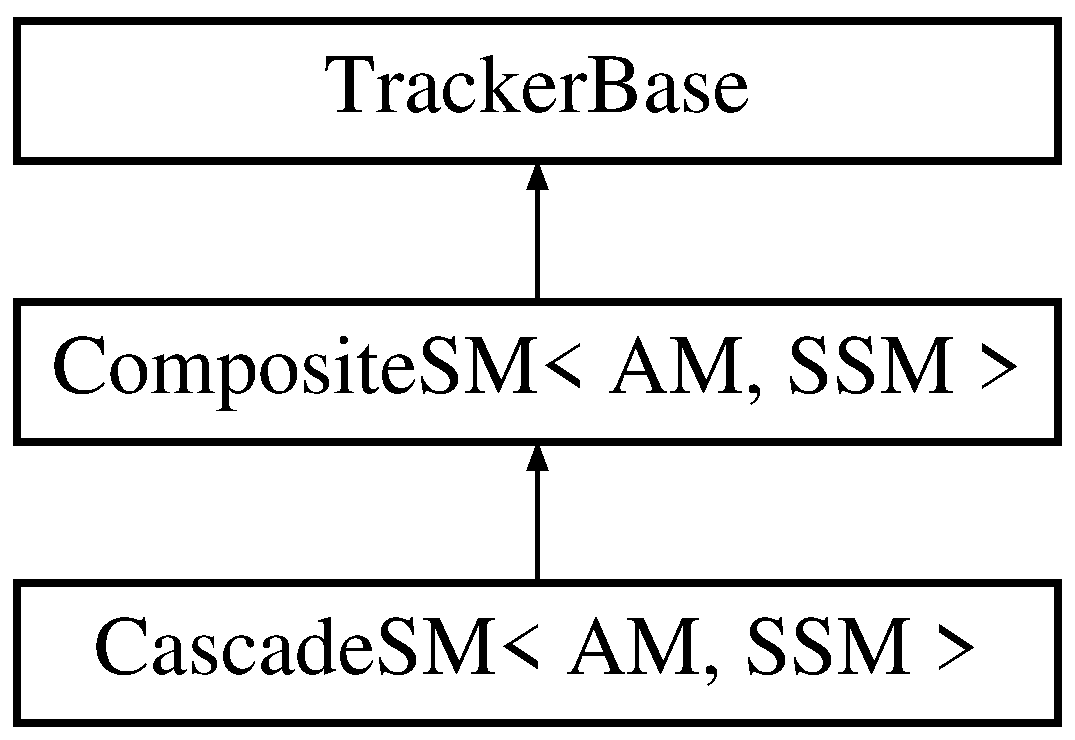
\includegraphics[height=3.000000cm]{classCascadeSM}
\end{center}
\end{figure}
\subsection*{Public Types}
\begin{DoxyCompactItemize}
\item 
\hypertarget{classCascadeSM_a2160669d0a3c681e6f6dd96daf67f3bc}{typedef \hyperlink{structCascadeParams}{Cascade\-Params} {\bfseries Param\-Type}}\label{classCascadeSM_a2160669d0a3c681e6f6dd96daf67f3bc}

\item 
\hypertarget{classCascadeSM_a5c5b6836ce4813905865b7e2b6abc034}{typedef S\-M\-::\-S\-S\-M\-Params {\bfseries S\-S\-M\-Params}}\label{classCascadeSM_a5c5b6836ce4813905865b7e2b6abc034}

\end{DoxyCompactItemize}
\subsection*{Public Member Functions}
\begin{DoxyCompactItemize}
\item 
\hypertarget{classCascadeSM_a513ca9d591958b20edd5578fe3e008ea}{{\bfseries Cascade\-S\-M} (const vector$<$ \hyperlink{classSearchMethod}{S\-M} $\ast$ $>$ \-\_\-trackers, const \hyperlink{structCascadeParams}{Param\-Type} $\ast$casc\-\_\-params)}\label{classCascadeSM_a513ca9d591958b20edd5578fe3e008ea}

\item 
\hypertarget{classCascadeSM_aaf5ad7cc2386611fc1fe89ee51b98be5}{void {\bfseries initialize} (const cv\-::\-Mat \&corners) override}\label{classCascadeSM_aaf5ad7cc2386611fc1fe89ee51b98be5}

\item 
\hypertarget{classCascadeSM_a259830554eba3cde05b22ac2987b0619}{void {\bfseries update} () override}\label{classCascadeSM_a259830554eba3cde05b22ac2987b0619}

\item 
\hypertarget{classCascadeSM_adb874c060f5afc2ad6f254d036982b66}{void {\bfseries set\-Image} (const cv\-::\-Mat \&img) override}\label{classCascadeSM_adb874c060f5afc2ad6f254d036982b66}

\item 
\hypertarget{classCascadeSM_a0e1062fb079385a9401f38c1d07ed973}{const cv\-::\-Mat \& {\bfseries get\-Region} () override}\label{classCascadeSM_a0e1062fb079385a9401f38c1d07ed973}

\item 
\hypertarget{classCascadeSM_a4da53dbe64b328cee42ebbea97ad312c}{void {\bfseries set\-Region} (const cv\-::\-Mat \&corners) override}\label{classCascadeSM_a4da53dbe64b328cee42ebbea97ad312c}

\end{DoxyCompactItemize}
\subsection*{Protected Member Functions}
\begin{DoxyCompactItemize}
\item 
\hypertarget{classCascadeSM_a103a9c3e9d7fd24d635a5e712ab63d5c}{void {\bfseries update\-Trackers} (const cv\-::\-Mat \&img)}\label{classCascadeSM_a103a9c3e9d7fd24d635a5e712ab63d5c}

\end{DoxyCompactItemize}
\subsection*{Protected Attributes}
\begin{DoxyCompactItemize}
\item 
\hypertarget{classCascadeSM_aa890250e26b0f2f63e374c4a1ca95633}{\hyperlink{structCascadeParams}{Param\-Type} {\bfseries params}}\label{classCascadeSM_aa890250e26b0f2f63e374c4a1ca95633}

\item 
\hypertarget{classCascadeSM_a968678d70af6c50ec1d5e6a975ad1b28}{bool {\bfseries failure\-\_\-detected}}\label{classCascadeSM_a968678d70af6c50ec1d5e6a975ad1b28}

\item 
\hypertarget{classCascadeSM_a171d626bc3fddb4d52858f1faa4eb10d}{vector$<$ cv\-::\-Mat $>$ {\bfseries img\-\_\-buffer}}\label{classCascadeSM_a171d626bc3fddb4d52858f1faa4eb10d}

\item 
\hypertarget{classCascadeSM_a28020796ab72ee542176e46d11d9b8ba}{vector$<$ cv\-::\-Mat $>$ {\bfseries corners\-\_\-buffer}}\label{classCascadeSM_a28020796ab72ee542176e46d11d9b8ba}

\item 
\hypertarget{classCascadeSM_a5718343c4985f1fc99cc8e042b3f4fd3}{int {\bfseries buffer\-\_\-id}}\label{classCascadeSM_a5718343c4985f1fc99cc8e042b3f4fd3}

\item 
\hypertarget{classCascadeSM_ae9f9bb3f7a8f1866f7d94d78b0606705}{bool {\bfseries buffer\-\_\-filled}}\label{classCascadeSM_ae9f9bb3f7a8f1866f7d94d78b0606705}

\item 
\hypertarget{classCascadeSM_a6193fd7ff22c2c4dfcf0522ac5921bce}{cv\-::\-Mat {\bfseries curr\-\_\-img}}\label{classCascadeSM_a6193fd7ff22c2c4dfcf0522ac5921bce}

\end{DoxyCompactItemize}


\subsection{Detailed Description}
\subsubsection*{template$<$class A\-M, class S\-S\-M$>$class Cascade\-S\-M$<$ A\-M, S\-S\-M $>$}

run multiple search methods in cascade with the same A\-M/\-S\-S\-M; although the code here is currently identical to \hyperlink{classCascadeTracker}{Cascade\-Tracker}, a seperate module exists for future extensions that take advantage of the additional information that is available to the Cascade through direct access to the underlying A\-M and S\-S\-M 

The documentation for this class was generated from the following file\-:\begin{DoxyCompactItemize}
\item 
S\-M/include/mtf/\-S\-M/Cascade\-S\-M.\-h\end{DoxyCompactItemize}

\hypertarget{classCascadeTracker}{\section{Cascade\-Tracker Class Reference}
\label{classCascadeTracker}\index{Cascade\-Tracker@{Cascade\-Tracker}}
}
Inheritance diagram for Cascade\-Tracker\-:\begin{figure}[H]
\begin{center}
\leavevmode
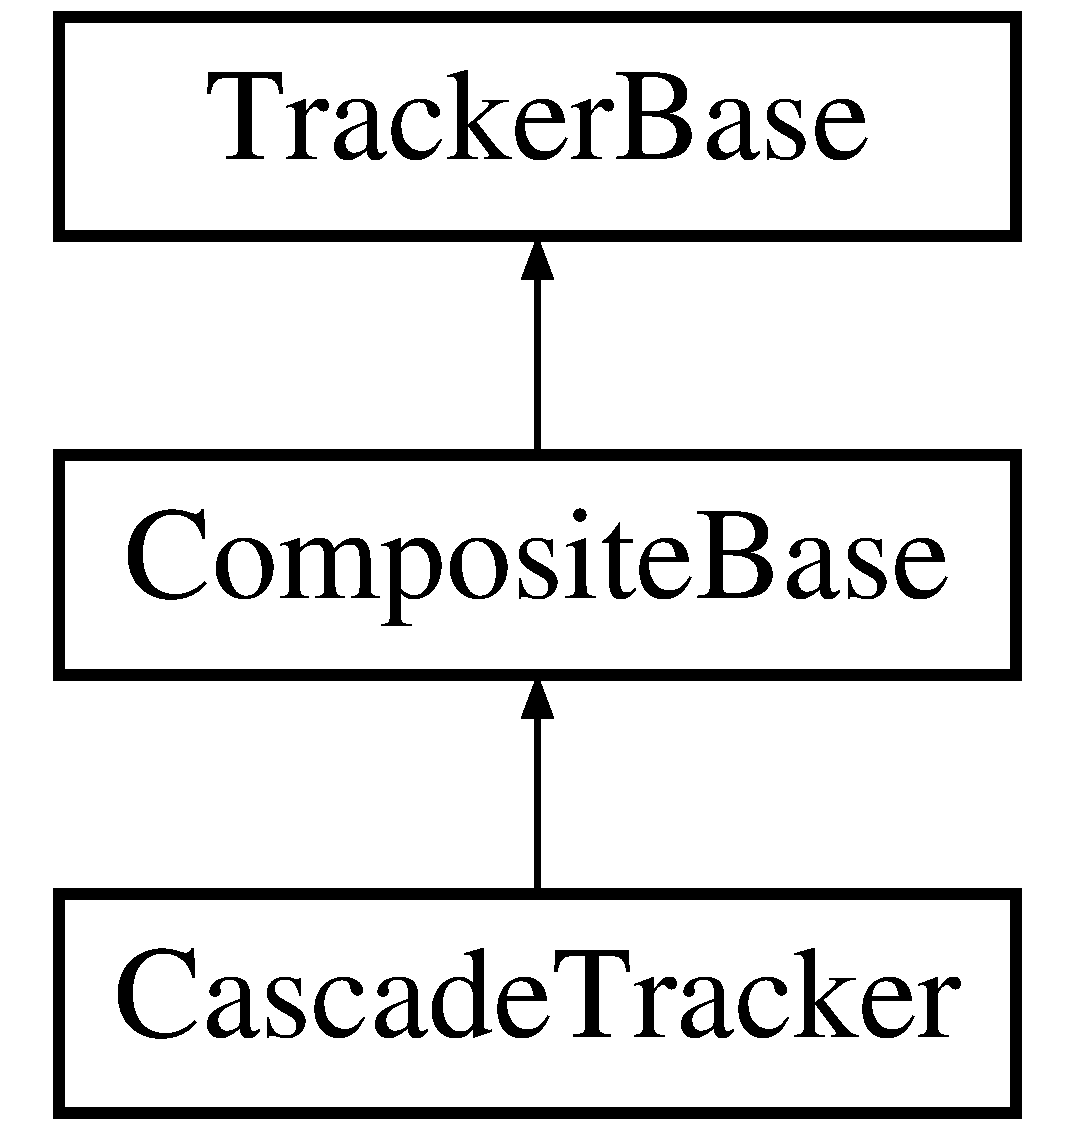
\includegraphics[height=3.000000cm]{classCascadeTracker}
\end{center}
\end{figure}
\subsection*{Public Types}
\begin{DoxyCompactItemize}
\item 
\hypertarget{classCascadeTracker_a950103310f4517611776669eae6ad803}{typedef \hyperlink{structCascadeParams}{Cascade\-Params} {\bfseries Param\-Type}}\label{classCascadeTracker_a950103310f4517611776669eae6ad803}

\end{DoxyCompactItemize}
\subsection*{Public Member Functions}
\begin{DoxyCompactItemize}
\item 
\hypertarget{classCascadeTracker_a18cdecc9ee0c781d72bbeda73038a348}{{\bfseries Cascade\-Tracker} (const vector$<$ Tracker\-Base $\ast$ $>$ \-\_\-trackers, const \hyperlink{structCascadeParams}{Param\-Type} $\ast$casc\-\_\-params)}\label{classCascadeTracker_a18cdecc9ee0c781d72bbeda73038a348}

\item 
\hypertarget{classCascadeTracker_ad6b9d0a494f3d2ff5709c6aa8f904b6b}{void {\bfseries initialize} (const cv\-::\-Mat \&corners) override}\label{classCascadeTracker_ad6b9d0a494f3d2ff5709c6aa8f904b6b}

\item 
\hypertarget{classCascadeTracker_afd3628c013327ebc70d6d63610cb26aa}{void {\bfseries update} () override}\label{classCascadeTracker_afd3628c013327ebc70d6d63610cb26aa}

\item 
\hypertarget{classCascadeTracker_a2c9d50442cadaa46f1632b4b8ea63fd2}{void {\bfseries set\-Region} (const cv\-::\-Mat \&corners) override}\label{classCascadeTracker_a2c9d50442cadaa46f1632b4b8ea63fd2}

\item 
\hypertarget{classCascadeTracker_a1b84edf12ac0bd425730c066883fa16a}{const cv\-::\-Mat \& {\bfseries get\-Region} () override}\label{classCascadeTracker_a1b84edf12ac0bd425730c066883fa16a}

\item 
\hypertarget{classCascadeTracker_a2e6a421c69864b8c565f324ab2a8aeb5}{void {\bfseries set\-Image} (const cv\-::\-Mat \&img) override}\label{classCascadeTracker_a2e6a421c69864b8c565f324ab2a8aeb5}

\end{DoxyCompactItemize}
\subsection*{Public Attributes}
\begin{DoxyCompactItemize}
\item 
\hypertarget{classCascadeTracker_a7e96165cef1fe1341a185c80dde82979}{\hyperlink{structCascadeParams}{Param\-Type} {\bfseries params}}\label{classCascadeTracker_a7e96165cef1fe1341a185c80dde82979}

\end{DoxyCompactItemize}
\subsection*{Protected Member Functions}
\begin{DoxyCompactItemize}
\item 
\hypertarget{classCascadeTracker_a45f0e405d48ee932856a29983160a6ec}{void {\bfseries update\-Trackers} (const cv\-::\-Mat \&img)}\label{classCascadeTracker_a45f0e405d48ee932856a29983160a6ec}

\end{DoxyCompactItemize}
\subsection*{Protected Attributes}
\begin{DoxyCompactItemize}
\item 
\hypertarget{classCascadeTracker_a9da79c51b90de7e14a3a27a662155992}{bool {\bfseries failure\-\_\-detected}}\label{classCascadeTracker_a9da79c51b90de7e14a3a27a662155992}

\item 
\hypertarget{classCascadeTracker_a079cfc88c81d9e2f79f7a47be0c8ac3b}{vector$<$ cv\-::\-Mat $>$ {\bfseries img\-\_\-buffer}}\label{classCascadeTracker_a079cfc88c81d9e2f79f7a47be0c8ac3b}

\item 
\hypertarget{classCascadeTracker_a05e5f93d0fe65947f95a77faa8bc9eae}{vector$<$ cv\-::\-Mat $>$ {\bfseries corners\-\_\-buffer}}\label{classCascadeTracker_a05e5f93d0fe65947f95a77faa8bc9eae}

\item 
\hypertarget{classCascadeTracker_ad574dce0ac9be291f0347f39ae5aaf43}{int {\bfseries buffer\-\_\-id}}\label{classCascadeTracker_ad574dce0ac9be291f0347f39ae5aaf43}

\item 
\hypertarget{classCascadeTracker_a75c5584ebb989e299907acb77100610e}{bool {\bfseries buffer\-\_\-filled}}\label{classCascadeTracker_a75c5584ebb989e299907acb77100610e}

\item 
\hypertarget{classCascadeTracker_ac534daf73fbb3c14aaaead07644b9e42}{cv\-::\-Mat {\bfseries curr\-\_\-img}}\label{classCascadeTracker_ac534daf73fbb3c14aaaead07644b9e42}

\end{DoxyCompactItemize}


The documentation for this class was generated from the following file\-:\begin{DoxyCompactItemize}
\item 
S\-M/include/mtf/\-S\-M/Cascade\-Tracker.\-h\end{DoxyCompactItemize}

\hypertarget{classCCRE}{\section{C\-C\-R\-E Class Reference}
\label{classCCRE}\index{C\-C\-R\-E@{C\-C\-R\-E}}
}


Cross Cumulative Residual Entropy.  




{\ttfamily \#include $<$C\-C\-R\-E.\-h$>$}

Inheritance diagram for C\-C\-R\-E\-:\begin{figure}[H]
\begin{center}
\leavevmode
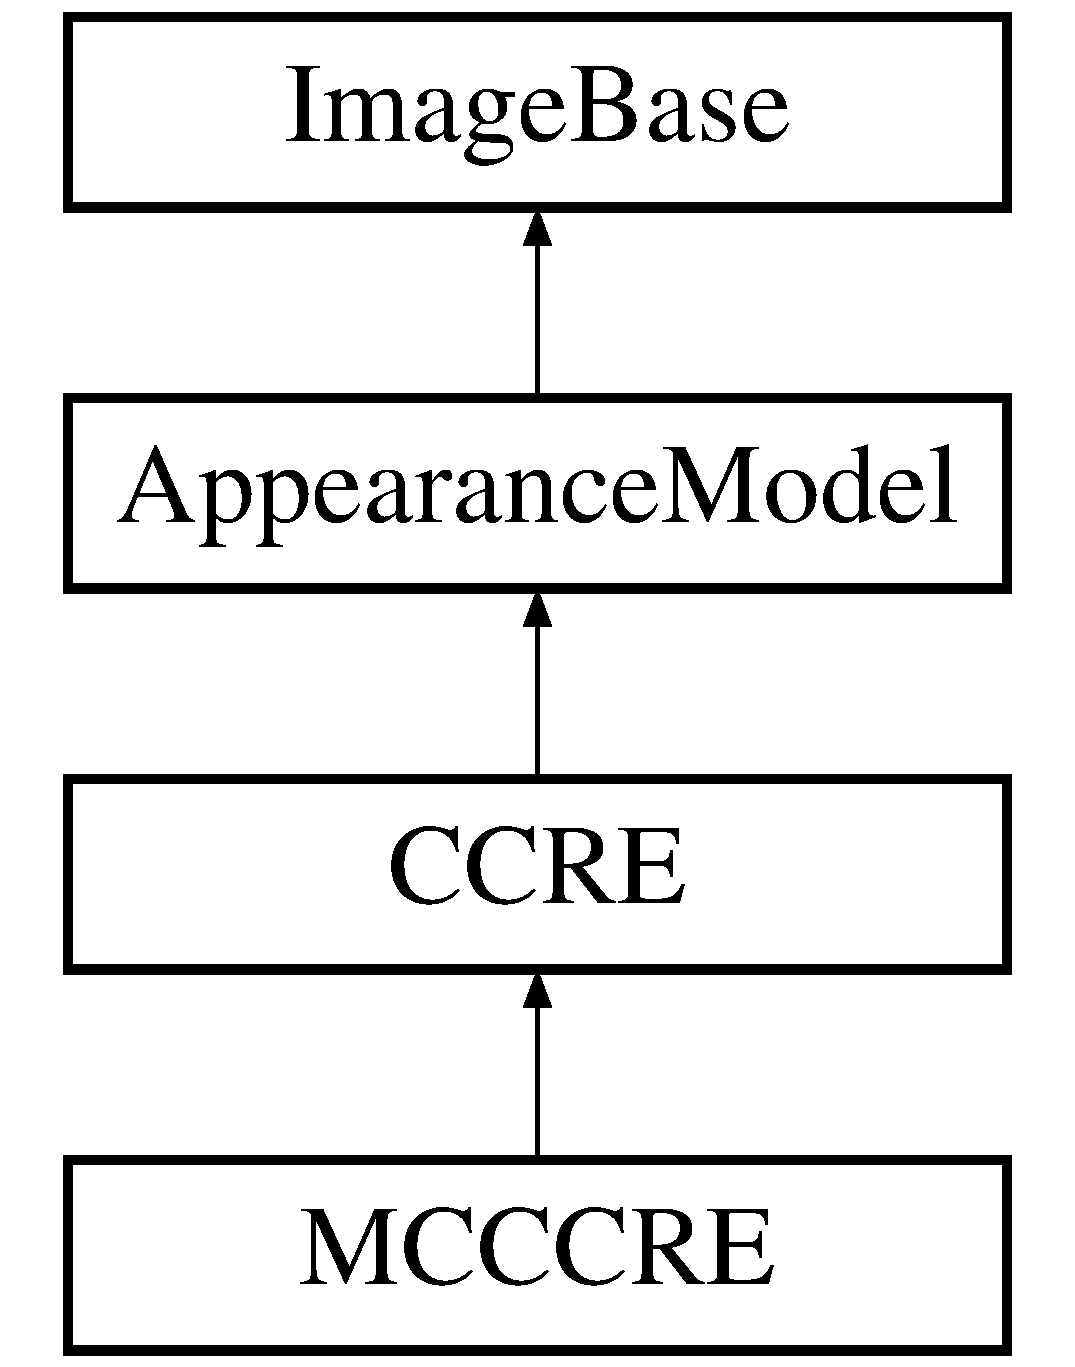
\includegraphics[height=4.000000cm]{classCCRE}
\end{center}
\end{figure}
\subsection*{Public Types}
\begin{DoxyCompactItemize}
\item 
\hypertarget{classCCRE_a3005dd4c7093c54a066347df2ecb7431}{typedef \hyperlink{structCCREParams}{C\-C\-R\-E\-Params} {\bfseries Param\-Type}}\label{classCCRE_a3005dd4c7093c54a066347df2ecb7431}

\item 
\hypertarget{classCCRE_ac55a39adcb2c002aff5260fa78f96b53}{typedef double {\bfseries Element\-Type}}\label{classCCRE_ac55a39adcb2c002aff5260fa78f96b53}

\item 
\hypertarget{classCCRE_a55c3a42bfa3b8ebcccd9c51e73f36394}{typedef double {\bfseries Result\-Type}}\label{classCCRE_a55c3a42bfa3b8ebcccd9c51e73f36394}

\end{DoxyCompactItemize}
\subsection*{Public Member Functions}
\begin{DoxyCompactItemize}
\item 
\hypertarget{classCCRE_adc57df943876cd0f20fc9d653d5b3acb}{{\bfseries C\-C\-R\-E} (const \hyperlink{structCCREParams}{Param\-Type} $\ast$ccre\-\_\-params=nullptr, int \-\_\-n\-\_\-channels=1)}\label{classCCRE_adc57df943876cd0f20fc9d653d5b3acb}

\item 
\hypertarget{classCCRE_a72851d2a7225768fac7e0f59e95cb99d}{double \hyperlink{classCCRE_a72851d2a7225768fac7e0f59e95cb99d}{get\-Likelihood} () const override}\label{classCCRE_a72851d2a7225768fac7e0f59e95cb99d}

\begin{DoxyCompactList}\small\item\em returns a normalized version of the similarity that lies between 0 and 1 and can be interpreted as the likelihood that the current patch represents the same object as the initial patch \end{DoxyCompactList}\item 
bool \hyperlink{classCCRE_a5ef4da8fc8c410bddaded394596169be}{is\-Symmetrical} () const override
\begin{DoxyCompactList}\small\item\em return false if the similarity function f is not symmetrical, i.\-e. \end{DoxyCompactList}\item 
void \hyperlink{classCCRE_aa108e906b98207bbb4b5eb86ca6f5bc8}{initialize\-Similarity} () override
\begin{DoxyCompactList}\small\item\em methods to initialize the state variables -\/ to be called once when the tracker is initialized. \end{DoxyCompactList}\item 
\hypertarget{classCCRE_a5d8901983d3383c05e0bc35de29a9656}{void {\bfseries initialize\-Grad} () override}\label{classCCRE_a5d8901983d3383c05e0bc35de29a9656}

\item 
void \hyperlink{classCCRE_ade5c18165416a3c179cadecab9df7712}{initialize\-Hess} () override
\begin{DoxyCompactList}\small\item\em even though the Hessian of the error norm w.\-r.\-t. \end{DoxyCompactList}\item 
void \hyperlink{classCCRE_a88f2514eb41b3a38278cca83c1b884dd}{update\-Similarity} (bool prereq\-\_\-only=1) override
\begin{DoxyCompactList}\small\item\em functions for updating state variables when a new image arrives \end{DoxyCompactList}\item 
\hypertarget{classCCRE_a52a2b20f5413ed69f5651eb2d8c88c21}{void {\bfseries update\-Init\-Grad} () override}\label{classCCRE_a52a2b20f5413ed69f5651eb2d8c88c21}

\item 
\hypertarget{classCCRE_ab28162c5805e25a9fe16c471e796ec39}{void {\bfseries update\-Curr\-Grad} () override}\label{classCCRE_ab28162c5805e25a9fe16c471e796ec39}

\item 
void \hyperlink{classCCRE_a2357913ffb5630de31b891c9847d1c0a}{cmpt\-Init\-Hessian} (Matrix\-Xd \&hessian, const Matrix\-Xd \&curr\-\_\-pix\-\_\-jacobian) override
\begin{DoxyCompactList}\small\item\em compute the S x S Hessian of the error norm using the supplied N x S Jacobian of pixel values w.\-r.\-t. \end{DoxyCompactList}\item 
\hypertarget{classCCRE_a09dfa7ac01a955a71c1f4a4fe2086411}{void {\bfseries cmpt\-Curr\-Hessian} (Matrix\-Xd \&hessian, const Matrix\-Xd \&curr\-\_\-pix\-\_\-jacobian) override}\label{classCCRE_a09dfa7ac01a955a71c1f4a4fe2086411}

\item 
\hypertarget{classCCRE_a9d4f059246c4eac4cacccd47f38a517f}{void \hyperlink{classCCRE_a9d4f059246c4eac4cacccd47f38a517f}{cmpt\-Init\-Hessian} (Matrix\-Xd \&init\-\_\-hessian, const Matrix\-Xd \&init\-\_\-pix\-\_\-jacobian, const Matrix\-Xd \&init\-\_\-pix\-\_\-hessian) override}\label{classCCRE_a9d4f059246c4eac4cacccd47f38a517f}

\begin{DoxyCompactList}\small\item\em compute the exact Hessian by considering the second order terms too \end{DoxyCompactList}\item 
\hypertarget{classCCRE_ad8f83bc4d5afc1425a1d9e6a7c6584d1}{void {\bfseries cmpt\-Curr\-Hessian} (Matrix\-Xd \&curr\-\_\-hessian, const Matrix\-Xd \&curr\-\_\-pix\-\_\-jacobian, const Matrix\-Xd \&curr\-\_\-pix\-\_\-hessian) override}\label{classCCRE_ad8f83bc4d5afc1425a1d9e6a7c6584d1}

\item 
\hypertarget{classCCRE_a1f10eb0fc8a53cb6f257cadc9e4af172}{void {\bfseries cmpt\-Self\-Hessian} (Matrix\-Xd \&self\-\_\-hessian, const Matrix\-Xd \&curr\-\_\-pix\-\_\-jacobian) override}\label{classCCRE_a1f10eb0fc8a53cb6f257cadc9e4af172}

\item 
\hypertarget{classCCRE_a657d200ec0aa7c0a41217ee02ed19fd7}{void {\bfseries cmpt\-Self\-Hessian} (Matrix\-Xd \&self\-\_\-hessian, const Matrix\-Xd \&curr\-\_\-pix\-\_\-jacobian, const Matrix\-Xd \&curr\-\_\-pix\-\_\-hessian) override}\label{classCCRE_a657d200ec0aa7c0a41217ee02ed19fd7}

\item 
\hypertarget{classCCRE_a217052773a5664d03548b20a0fc41f2f}{void \hyperlink{classCCRE_a217052773a5664d03548b20a0fc41f2f}{initialize\-Dist\-Feat} () override}\label{classCCRE_a217052773a5664d03548b20a0fc41f2f}

\begin{DoxyCompactList}\small\item\em to be called once during initialization if any of the distance feature functionality is to be used \end{DoxyCompactList}\item 
void \hyperlink{classCCRE_a102becb1188b7408863bc2036b07b079}{update\-Dist\-Feat} () override
\begin{DoxyCompactList}\small\item\em computes a \char`\"{}distance\char`\"{} vector using the current image patch such that, when the distance vectors corresponding to two patches are passed to the distance operator above, it uses these to compute a scalar that measures the distance or dissimilarity between the two patches; this distance vector should be designed so as to offload as much computation as possible from the distance operator, i.\-e. \end{DoxyCompactList}\item 
\hypertarget{classCCRE_a74605d82644df1e0407288900b8af4f8}{const double $\ast$ {\bfseries get\-Dist\-Feat} () override}\label{classCCRE_a74605d82644df1e0407288900b8af4f8}

\item 
\hypertarget{classCCRE_a1abb4b695361b138deb6b8f3b056bcbc}{void \hyperlink{classCCRE_a1abb4b695361b138deb6b8f3b056bcbc}{update\-Dist\-Feat} (double $\ast$feat\-\_\-addr) override}\label{classCCRE_a1abb4b695361b138deb6b8f3b056bcbc}

\begin{DoxyCompactList}\small\item\em overloaded version to write the distance feature directly to a row (or column) of a matrix storing the distance features corresponding to several patches; \end{DoxyCompactList}\item 
\hypertarget{classCCRE_a661e2c1055913da2b72432d0e0bba590}{double \hyperlink{classCCRE_a661e2c1055913da2b72432d0e0bba590}{operator()} (const double $\ast$hist1\-\_\-mat\-\_\-addr, const double $\ast$hist2\-\_\-mat\-\_\-addr, size\-\_\-t hist\-\_\-mat\-\_\-size, double worst\-\_\-dist=-\/1) const override}\label{classCCRE_a661e2c1055913da2b72432d0e0bba590}

\begin{DoxyCompactList}\small\item\em computes the distance / dissimilarity between two patches where each is codified or represented by a suitable distance feature computed using update\-Dist\-Feat \end{DoxyCompactList}\item 
\hypertarget{classCCRE_a5ead9c9e9298c6f666b0134b3baa2225}{int \hyperlink{classCCRE_a5ead9c9e9298c6f666b0134b3baa2225}{get\-Dist\-Feat\-Size} () override}\label{classCCRE_a5ead9c9e9298c6f666b0134b3baa2225}

\begin{DoxyCompactList}\small\item\em returns the size of the distance vector \end{DoxyCompactList}\end{DoxyCompactItemize}
\subsection*{Public Attributes}
\begin{DoxyCompactItemize}
\item 
\hypertarget{classCCRE_a7e74137f7fd5f83e5cb831813157102a}{\hyperlink{structCCREParams}{Param\-Type} {\bfseries params}}\label{classCCRE_a7e74137f7fd5f83e5cb831813157102a}

\item 
\hypertarget{classCCRE_a0d172170d85e26d8eda32b889b0af245}{int {\bfseries feat\-\_\-size}}\label{classCCRE_a0d172170d85e26d8eda32b889b0af245}

\item 
\hypertarget{classCCRE_af97657776d1263aa1ba31aed2c0c86ed}{Vector\-Xd {\bfseries feat\-\_\-vec}}\label{classCCRE_af97657776d1263aa1ba31aed2c0c86ed}

\end{DoxyCompactItemize}
\subsection*{Protected Member Functions}
\begin{DoxyCompactItemize}
\item 
\hypertarget{classCCRE_a3601a5e879139e69558e9d88291f4645}{void {\bfseries update\-Sym\-Similarity} (bool prereq\-\_\-only)}\label{classCCRE_a3601a5e879139e69558e9d88291f4645}

\item 
\hypertarget{classCCRE_a6652e68a3221c69bd2bc830cdd32182f}{void {\bfseries update\-Sym\-Init\-Grad} ()}\label{classCCRE_a6652e68a3221c69bd2bc830cdd32182f}

\item 
\hypertarget{classCCRE_acdb7a48305fe90c59a1cfa32c7e31fc6}{void {\bfseries cmpt\-Sym\-Init\-Hessian} (Matrix\-Xd \&hessian, const Matrix\-Xd \&curr\-\_\-pix\-\_\-jacobian)}\label{classCCRE_acdb7a48305fe90c59a1cfa32c7e31fc6}

\item 
\hypertarget{classCCRE_a5ba97f2ce7f3f571c76f042de7557562}{void {\bfseries cmpt\-Cum\-Self\-Hist} ()}\label{classCCRE_a5ba97f2ce7f3f571c76f042de7557562}

\end{DoxyCompactItemize}
\subsection*{Protected Attributes}
\begin{DoxyCompactItemize}
\item 
\hypertarget{classCCRE_a546c521ce21bb460cfbba80216735a5b}{double {\bfseries max\-\_\-similarity}}\label{classCCRE_a546c521ce21bb460cfbba80216735a5b}

\item 
\hypertarget{classCCRE_ac4c475d6fec27db6f8522da1e803443a}{double \hyperlink{classCCRE_ac4c475d6fec27db6f8522da1e803443a}{hist\-\_\-pre\-\_\-seed}}\label{classCCRE_ac4c475d6fec27db6f8522da1e803443a}

\begin{DoxyCompactList}\small\item\em value with which to preseed the individual histograms \end{DoxyCompactList}\item 
\hypertarget{classCCRE_afc96a1d02a189c32d3ef78cf79c4dae5}{double \hyperlink{classCCRE_afc96a1d02a189c32d3ef78cf79c4dae5}{hist\-\_\-norm\-\_\-mult}}\label{classCCRE_afc96a1d02a189c32d3ef78cf79c4dae5}

\begin{DoxyCompactList}\small\item\em multiplicative factor for normalizing histograms \end{DoxyCompactList}\item 
\hypertarget{classCCRE_aa0a39232ee88f1526e5404c0fdf8495a}{int {\bfseries joint\-\_\-hist\-\_\-size}}\label{classCCRE_aa0a39232ee88f1526e5404c0fdf8495a}

\item 
\hypertarget{classCCRE_a4277fca9c76ece7b115f2233d9147ed4}{double {\bfseries log\-\_\-hist\-\_\-norm\-\_\-mult}}\label{classCCRE_a4277fca9c76ece7b115f2233d9147ed4}

\item 
\hypertarget{classCCRE_a33d8fc22570e6953bb3a354e208a1f02}{Vector\-Xd \hyperlink{classCCRE_a33d8fc22570e6953bb3a354e208a1f02}{init\-\_\-hist}}\label{classCCRE_a33d8fc22570e6953bb3a354e208a1f02}

\begin{DoxyCompactList}\small\item\em n\-\_\-bins x n\-\_\-bins joint histograms; \end{DoxyCompactList}\item 
\hypertarget{classCCRE_a4e9702f1e4d81f0ed0190b2062d2bfcc}{Vector\-Xd {\bfseries curr\-\_\-hist}}\label{classCCRE_a4e9702f1e4d81f0ed0190b2062d2bfcc}

\item 
\hypertarget{classCCRE_a2c43cee0ffbb540dd735d8ce805942a2}{Vector\-Xd {\bfseries init\-\_\-cum\-\_\-hist}}\label{classCCRE_a2c43cee0ffbb540dd735d8ce805942a2}

\item 
\hypertarget{classCCRE_af8538160dbb6848eee1b6cd9b1f4e788}{Vector\-Xd {\bfseries curr\-\_\-cum\-\_\-hist}}\label{classCCRE_af8538160dbb6848eee1b6cd9b1f4e788}

\item 
\hypertarget{classCCRE_aaba3d5a34118b0294dd716b39fec2023}{Matrix\-Xd {\bfseries init\-\_\-hist\-\_\-mat}}\label{classCCRE_aaba3d5a34118b0294dd716b39fec2023}

\item 
\hypertarget{classCCRE_aa156f513feb2faac94befeba89efe10e}{Matrix\-Xd {\bfseries curr\-\_\-hist\-\_\-mat}}\label{classCCRE_aa156f513feb2faac94befeba89efe10e}

\item 
\hypertarget{classCCRE_adbc7633506a0567f791cbae97e69cfbf}{Matrix\-Xd {\bfseries init\-\_\-cum\-\_\-hist\-\_\-mat}}\label{classCCRE_adbc7633506a0567f791cbae97e69cfbf}

\item 
\hypertarget{classCCRE_a7d4cb88fcd5fd88a7132de4a538a4bfb}{Matrix\-Xd {\bfseries curr\-\_\-cum\-\_\-hist\-\_\-mat}}\label{classCCRE_a7d4cb88fcd5fd88a7132de4a538a4bfb}

\item 
\hypertarget{classCCRE_a481007f939c43ae813a3a4d222fd0852}{Matrix\-Xd {\bfseries cum\-\_\-joint\-\_\-hist}}\label{classCCRE_a481007f939c43ae813a3a4d222fd0852}

\item 
\hypertarget{classCCRE_a09ce115f1eb533a2a7532672cd85d218}{Matrix\-Xd \hyperlink{classCCRE_a09ce115f1eb533a2a7532672cd85d218}{init\-\_\-hist\-\_\-grad}}\label{classCCRE_a09ce115f1eb533a2a7532672cd85d218}

\begin{DoxyCompactList}\small\item\em n\-\_\-bins X N gradients of the marginal histograms w.\-r.\-t. pixel values \end{DoxyCompactList}\item 
\hypertarget{classCCRE_a9282d15b8d7022acb34b1d3818fb95bb}{Matrix\-Xd {\bfseries curr\-\_\-hist\-\_\-grad}}\label{classCCRE_a9282d15b8d7022acb34b1d3818fb95bb}

\item 
\hypertarget{classCCRE_acef298fae49c3d1468d2eb6b06ad70ef}{Matrix\-Xd {\bfseries init\-\_\-cum\-\_\-hist\-\_\-grad}}\label{classCCRE_acef298fae49c3d1468d2eb6b06ad70ef}

\item 
\hypertarget{classCCRE_aa10af4a3b8ed62f174274c4b61f0696a}{Matrix\-Xd {\bfseries curr\-\_\-cum\-\_\-hist\-\_\-grad}}\label{classCCRE_aa10af4a3b8ed62f174274c4b61f0696a}

\item 
\hypertarget{classCCRE_adea408b52017021834f32627ec414d0e}{Matrix\-Xd {\bfseries init\-\_\-hist\-\_\-hess}}\label{classCCRE_adea408b52017021834f32627ec414d0e}

\item 
\hypertarget{classCCRE_a910480195c78dfdf3f4646824a31775e}{Matrix\-Xd {\bfseries curr\-\_\-hist\-\_\-hess}}\label{classCCRE_a910480195c78dfdf3f4646824a31775e}

\item 
\hypertarget{classCCRE_ae31b16cb8fffb353705b76e36c144daf}{Matrix\-Xd {\bfseries init\-\_\-cum\-\_\-hist\-\_\-hess}}\label{classCCRE_ae31b16cb8fffb353705b76e36c144daf}

\item 
\hypertarget{classCCRE_ae465fffc2324511111fd44f22737f046}{Matrix\-Xd {\bfseries curr\-\_\-cum\-\_\-hist\-\_\-hess}}\label{classCCRE_ae465fffc2324511111fd44f22737f046}

\item 
\hypertarget{classCCRE_a2f4c80f752c9a6a1629639259b7f77e1}{Matrix\-Xd \hyperlink{classCCRE_a2f4c80f752c9a6a1629639259b7f77e1}{init\-\_\-cum\-\_\-joint\-\_\-hist\-\_\-grad}}\label{classCCRE_a2f4c80f752c9a6a1629639259b7f77e1}

\begin{DoxyCompactList}\small\item\em (n\-\_\-bins$\ast$n\-\_\-bins) X N gradients of the (flattened) current joint histogram w.\-r.\-t. initial and current pixel values \end{DoxyCompactList}\item 
\hypertarget{classCCRE_a45c2e08608fc6abcae306ced54cc5a74}{Matrix\-Xd {\bfseries curr\-\_\-cum\-\_\-joint\-\_\-hist\-\_\-grad}}\label{classCCRE_a45c2e08608fc6abcae306ced54cc5a74}

\item 
\hypertarget{classCCRE_adb2310a4d06be52d31d1f958e8a829ef}{Matrix\-Xd {\bfseries ccre\-\_\-log\-\_\-term}}\label{classCCRE_adb2310a4d06be52d31d1f958e8a829ef}

\item 
\hypertarget{classCCRE_ae8d74b675f6a0cac46ed821fe760c6ea}{Matrix\-Xd {\bfseries init\-\_\-hess\-\_\-factor}}\label{classCCRE_ae8d74b675f6a0cac46ed821fe760c6ea}

\item 
\hypertarget{classCCRE_a8cbe93ea74773cdf0ede899b85b02654}{Matrix\-Xd {\bfseries cum\-\_\-hess\-\_\-factor}}\label{classCCRE_a8cbe93ea74773cdf0ede899b85b02654}

\item 
\hypertarget{classCCRE_a710bedd5b90610c74fe55525c3724bcd}{Matrix\-Xd {\bfseries init\-\_\-hist\-\_\-grad\-\_\-ratio}}\label{classCCRE_a710bedd5b90610c74fe55525c3724bcd}

\item 
\hypertarget{classCCRE_aedab53e6fff99eb49a1b0cf28a35a758}{Matrix\-Xd {\bfseries cum\-\_\-hist\-\_\-grad\-\_\-ratio}}\label{classCCRE_aedab53e6fff99eb49a1b0cf28a35a758}

\item 
\hypertarget{classCCRE_a732fb8e068e7f25de6a507b427fb6210}{Matrix\-Xd {\bfseries init\-\_\-hist\-\_\-hess\-\_\-ratio}}\label{classCCRE_a732fb8e068e7f25de6a507b427fb6210}

\item 
\hypertarget{classCCRE_ac906668e7ee64d311abe8174adf13f75}{Matrix\-Xd {\bfseries cum\-\_\-hist\-\_\-hess\-\_\-ratio}}\label{classCCRE_ac906668e7ee64d311abe8174adf13f75}

\item 
\hypertarget{classCCRE_a8100a8b209a18bc7173b3c6115eb50fc}{Vector\-Xd {\bfseries init\-\_\-hist\-\_\-log}}\label{classCCRE_a8100a8b209a18bc7173b3c6115eb50fc}

\item 
\hypertarget{classCCRE_af4197c77ed7f45d4403c7d7c5516347c}{Vector\-Xd {\bfseries curr\-\_\-hist\-\_\-log}}\label{classCCRE_af4197c77ed7f45d4403c7d7c5516347c}

\item 
\hypertarget{classCCRE_a4234dd16c7f0c40483363bcc4ed29ccd}{Vector\-Xd {\bfseries init\-\_\-cum\-\_\-hist\-\_\-log}}\label{classCCRE_a4234dd16c7f0c40483363bcc4ed29ccd}

\item 
\hypertarget{classCCRE_a776439467de445d05da1012427bae80c}{Vector\-Xd {\bfseries curr\-\_\-cum\-\_\-hist\-\_\-log}}\label{classCCRE_a776439467de445d05da1012427bae80c}

\item 
\hypertarget{classCCRE_ad8bb30e4ea7c51076d1fab82ce844dbf}{Matrix\-Xd {\bfseries cum\-\_\-joint\-\_\-hist\-\_\-log}}\label{classCCRE_ad8bb30e4ea7c51076d1fab82ce844dbf}

\item 
\hypertarget{classCCRE_aa3bd03550ddfdea720e7b4017cdfad38}{Vector\-Xd {\bfseries cum\-\_\-joint\-\_\-hist\-\_\-sum}}\label{classCCRE_aa3bd03550ddfdea720e7b4017cdfad38}

\item 
\hypertarget{classCCRE_a7821bb023f4a60221219c8a4c69b7351}{Matrix\-Xd {\bfseries self\-\_\-cum\-\_\-joint\-\_\-hist}}\label{classCCRE_a7821bb023f4a60221219c8a4c69b7351}

\item 
\hypertarget{classCCRE_ac5c4d91774b512e82050e5d95e2fa5c0}{Matrix\-Xd {\bfseries self\-\_\-cum\-\_\-joint\-\_\-hist\-\_\-log}}\label{classCCRE_ac5c4d91774b512e82050e5d95e2fa5c0}

\item 
\hypertarget{classCCRE_a394cc5c5aded9439b9e7c1023f9a4e13}{Matrix\-Xd {\bfseries self\-\_\-ccre\-\_\-log\-\_\-term}}\label{classCCRE_a394cc5c5aded9439b9e7c1023f9a4e13}

\item 
\hypertarget{classCCRE_af7db10318c583dfa60f3d00e65f7a65d}{Matrix\-X2i \hyperlink{classCCRE_af7db10318c583dfa60f3d00e65f7a65d}{\-\_\-std\-\_\-bspl\-\_\-ids}}\label{classCCRE_af7db10318c583dfa60f3d00e65f7a65d}

\begin{DoxyCompactList}\small\item\em only used internally to increase speed by offlining as many computations as possible; \end{DoxyCompactList}\item 
\hypertarget{classCCRE_ae1f206752f925899335da36ab1dbef7b}{Matrix\-X2i {\bfseries \-\_\-init\-\_\-bspl\-\_\-ids}}\label{classCCRE_ae1f206752f925899335da36ab1dbef7b}

\item 
\hypertarget{classCCRE_ae8249f1cf2323c20a61963e812cf4aa9}{Matrix\-X2i {\bfseries \-\_\-curr\-\_\-bspl\-\_\-ids}}\label{classCCRE_ae8249f1cf2323c20a61963e812cf4aa9}

\item 
\hypertarget{classCCRE_a2eb5400ff35dd0c5bea7198ee61c5064}{Matrix\-Xi {\bfseries \-\_\-linear\-\_\-idx}}\label{classCCRE_a2eb5400ff35dd0c5bea7198ee61c5064}

\item 
\hypertarget{classCCRE_a5262075e3786ea02afdb30629e4466ce}{Matrix\-Xi {\bfseries \-\_\-linear\-\_\-idx2}}\label{classCCRE_a5262075e3786ea02afdb30629e4466ce}

\item 
\hypertarget{classCCRE_abde50706b47156bf8869a06c06717978}{Matrix\-X2i {\bfseries block\-\_\-extents}}\label{classCCRE_abde50706b47156bf8869a06c06717978}

\item 
\hypertarget{classCCRE_ae65b69a35d1b40650f5224fa9937bfb7}{char $\ast$ {\bfseries log\-\_\-fname}}\label{classCCRE_ae65b69a35d1b40650f5224fa9937bfb7}

\item 
\hypertarget{classCCRE_aa8e549ac84b7ecb99ac327625d650e2c}{char $\ast$ {\bfseries time\-\_\-fname}}\label{classCCRE_aa8e549ac84b7ecb99ac327625d650e2c}

\end{DoxyCompactItemize}


\subsection{Detailed Description}
Cross Cumulative Residual Entropy. 

\subsection{Member Function Documentation}
\hypertarget{classCCRE_a2357913ffb5630de31b891c9847d1c0a}{\index{C\-C\-R\-E@{C\-C\-R\-E}!cmpt\-Init\-Hessian@{cmpt\-Init\-Hessian}}
\index{cmpt\-Init\-Hessian@{cmpt\-Init\-Hessian}!CCRE@{C\-C\-R\-E}}
\subsubsection[{cmpt\-Init\-Hessian}]{\setlength{\rightskip}{0pt plus 5cm}void C\-C\-R\-E\-::cmpt\-Init\-Hessian (
\begin{DoxyParamCaption}
\item[{Matrix\-Xd \&}]{d2f\-\_\-dp2, }
\item[{const Matrix\-Xd \&}]{d\-I0\-\_\-dpssm}
\end{DoxyParamCaption}
)\hspace{0.3cm}{\ttfamily [override]}, {\ttfamily [virtual]}}}\label{classCCRE_a2357913ffb5630de31b891c9847d1c0a}


compute the S x S Hessian of the error norm using the supplied N x S Jacobian of pixel values w.\-r.\-t. 

external parameters; compute the approximate Hessian by ignoring the second order terms 

Reimplemented from \hyperlink{classAppearanceModel_ab153b47d09f121796d3f411626a5321c}{Appearance\-Model}.

\hypertarget{classCCRE_ade5c18165416a3c179cadecab9df7712}{\index{C\-C\-R\-E@{C\-C\-R\-E}!initialize\-Hess@{initialize\-Hess}}
\index{initialize\-Hess@{initialize\-Hess}!CCRE@{C\-C\-R\-E}}
\subsubsection[{initialize\-Hess}]{\setlength{\rightskip}{0pt plus 5cm}void C\-C\-R\-E\-::initialize\-Hess (
\begin{DoxyParamCaption}
{}
\end{DoxyParamCaption}
)\hspace{0.3cm}{\ttfamily [override]}, {\ttfamily [virtual]}}}\label{classCCRE_ade5c18165416a3c179cadecab9df7712}


even though the Hessian of the error norm w.\-r.\-t. 

pixel values is not a state variable (since it does not need to be computed separately to get the Hessian w.\-r.\-t S\-S\-M), this function is provided as a place to perform any one-\/time computations that may help to decrease the runtime cost of the interfacing function that computes this Hessian 

Reimplemented from \hyperlink{classAppearanceModel_afb47df1d5e8a74f41ac70af3612180d2}{Appearance\-Model}.

\hypertarget{classCCRE_aa108e906b98207bbb4b5eb86ca6f5bc8}{\index{C\-C\-R\-E@{C\-C\-R\-E}!initialize\-Similarity@{initialize\-Similarity}}
\index{initialize\-Similarity@{initialize\-Similarity}!CCRE@{C\-C\-R\-E}}
\subsubsection[{initialize\-Similarity}]{\setlength{\rightskip}{0pt plus 5cm}void C\-C\-R\-E\-::initialize\-Similarity (
\begin{DoxyParamCaption}
{}
\end{DoxyParamCaption}
)\hspace{0.3cm}{\ttfamily [override]}, {\ttfamily [virtual]}}}\label{classCCRE_aa108e906b98207bbb4b5eb86ca6f5bc8}


methods to initialize the state variables -\/ to be called once when the tracker is initialized. 

if any of these are reimplemented, there should be a statement there copying the computed value in the \char`\"{}init\char`\"{} variable to the corresponding \char`\"{}curr\char`\"{} variable so the two have the same value after this function is called;

Note for the S\-M\-: the \char`\"{}initialize\char`\"{} function for any state variable whose \char`\"{}update\char`\"{} function will be called later should be called once from the S\-M's own initialize function even if the initial value of that variable will not be used later; this is because updating the state variable may involve some computations which need to be performed only once and the A\-M is free to delegate any such computations to the respective \char`\"{}initialize\char`\"{} function to avoid repeating them in the \char`\"{}update\char`\"{} function which can have a negative impact on performance; thus if this function is not called, the results of these computations that are needed by the \char`\"{}update\char`\"{} function will remain uncomputed leading to undefined behavior;

also the initialize functions have a boolean indicator parameter called \char`\"{}is\-\_\-initialized\char`\"{} which defaults to true but should be set to false if they are called only to update the internal state to take into account any changes to the initial template, i.\-e. if they are called again after the first call to initialize the state (when it should be left to true) 

Reimplemented from \hyperlink{classAppearanceModel_abcd79170a5fccc0e9aa10675404ad655}{Appearance\-Model}.

\hypertarget{classCCRE_a5ef4da8fc8c410bddaded394596169be}{\index{C\-C\-R\-E@{C\-C\-R\-E}!is\-Symmetrical@{is\-Symmetrical}}
\index{is\-Symmetrical@{is\-Symmetrical}!CCRE@{C\-C\-R\-E}}
\subsubsection[{is\-Symmetrical}]{\setlength{\rightskip}{0pt plus 5cm}bool C\-C\-R\-E\-::is\-Symmetrical (
\begin{DoxyParamCaption}
{}
\end{DoxyParamCaption}
) const\hspace{0.3cm}{\ttfamily [inline]}, {\ttfamily [override]}, {\ttfamily [virtual]}}}\label{classCCRE_a5ef4da8fc8c410bddaded394596169be}


return false if the similarity function f is not symmetrical, i.\-e. 

f(a,b) != f(b, a); also applies to the distance functor so the two should be consistent; 

Reimplemented from \hyperlink{classAppearanceModel_a432b2d068bf735abfa58c023773e1721}{Appearance\-Model}.

\hypertarget{classCCRE_a102becb1188b7408863bc2036b07b079}{\index{C\-C\-R\-E@{C\-C\-R\-E}!update\-Dist\-Feat@{update\-Dist\-Feat}}
\index{update\-Dist\-Feat@{update\-Dist\-Feat}!CCRE@{C\-C\-R\-E}}
\subsubsection[{update\-Dist\-Feat}]{\setlength{\rightskip}{0pt plus 5cm}void C\-C\-R\-E\-::update\-Dist\-Feat (
\begin{DoxyParamCaption}
{}
\end{DoxyParamCaption}
)\hspace{0.3cm}{\ttfamily [inline]}, {\ttfamily [override]}, {\ttfamily [virtual]}}}\label{classCCRE_a102becb1188b7408863bc2036b07b079}


computes a \char`\"{}distance\char`\"{} vector using the current image patch such that, when the distance vectors corresponding to two patches are passed to the distance operator above, it uses these to compute a scalar that measures the distance or dissimilarity between the two patches; this distance vector should be designed so as to offload as much computation as possible from the distance operator, i.\-e. 

every computation that depends only on the current patch should be performed here and the results should be stored, suitably coded, in the distannce vector where they will be decoded and used to compute the distance measure 

Reimplemented from \hyperlink{classAppearanceModel_afc815587980df0cd28412a2cd1670854}{Appearance\-Model}.

\hypertarget{classCCRE_a88f2514eb41b3a38278cca83c1b884dd}{\index{C\-C\-R\-E@{C\-C\-R\-E}!update\-Similarity@{update\-Similarity}}
\index{update\-Similarity@{update\-Similarity}!CCRE@{C\-C\-R\-E}}
\subsubsection[{update\-Similarity}]{\setlength{\rightskip}{0pt plus 5cm}void C\-C\-R\-E\-::update\-Similarity (
\begin{DoxyParamCaption}
\item[{bool}]{prereq\-\_\-only = {\ttfamily 1}}
\end{DoxyParamCaption}
)\hspace{0.3cm}{\ttfamily [override]}, {\ttfamily [virtual]}}}\label{classCCRE_a88f2514eb41b3a38278cca83c1b884dd}


functions for updating state variables when a new image arrives 

prereq\-\_\-only should be left to true if update is only called to compute the prerequisites for the two gradient functions and the actual value of similarity is not needed 

Reimplemented from \hyperlink{classAppearanceModel_a06136ecd903e85ed2007da2c7b12bd58}{Appearance\-Model}.



The documentation for this class was generated from the following file\-:\begin{DoxyCompactItemize}
\item 
A\-M/include/mtf/\-A\-M/C\-C\-R\-E.\-h\end{DoxyCompactItemize}

\hypertarget{structCCREParams}{\section{C\-C\-R\-E\-Params Struct Reference}
\label{structCCREParams}\index{C\-C\-R\-E\-Params@{C\-C\-R\-E\-Params}}
}
Inheritance diagram for C\-C\-R\-E\-Params\-:\begin{figure}[H]
\begin{center}
\leavevmode
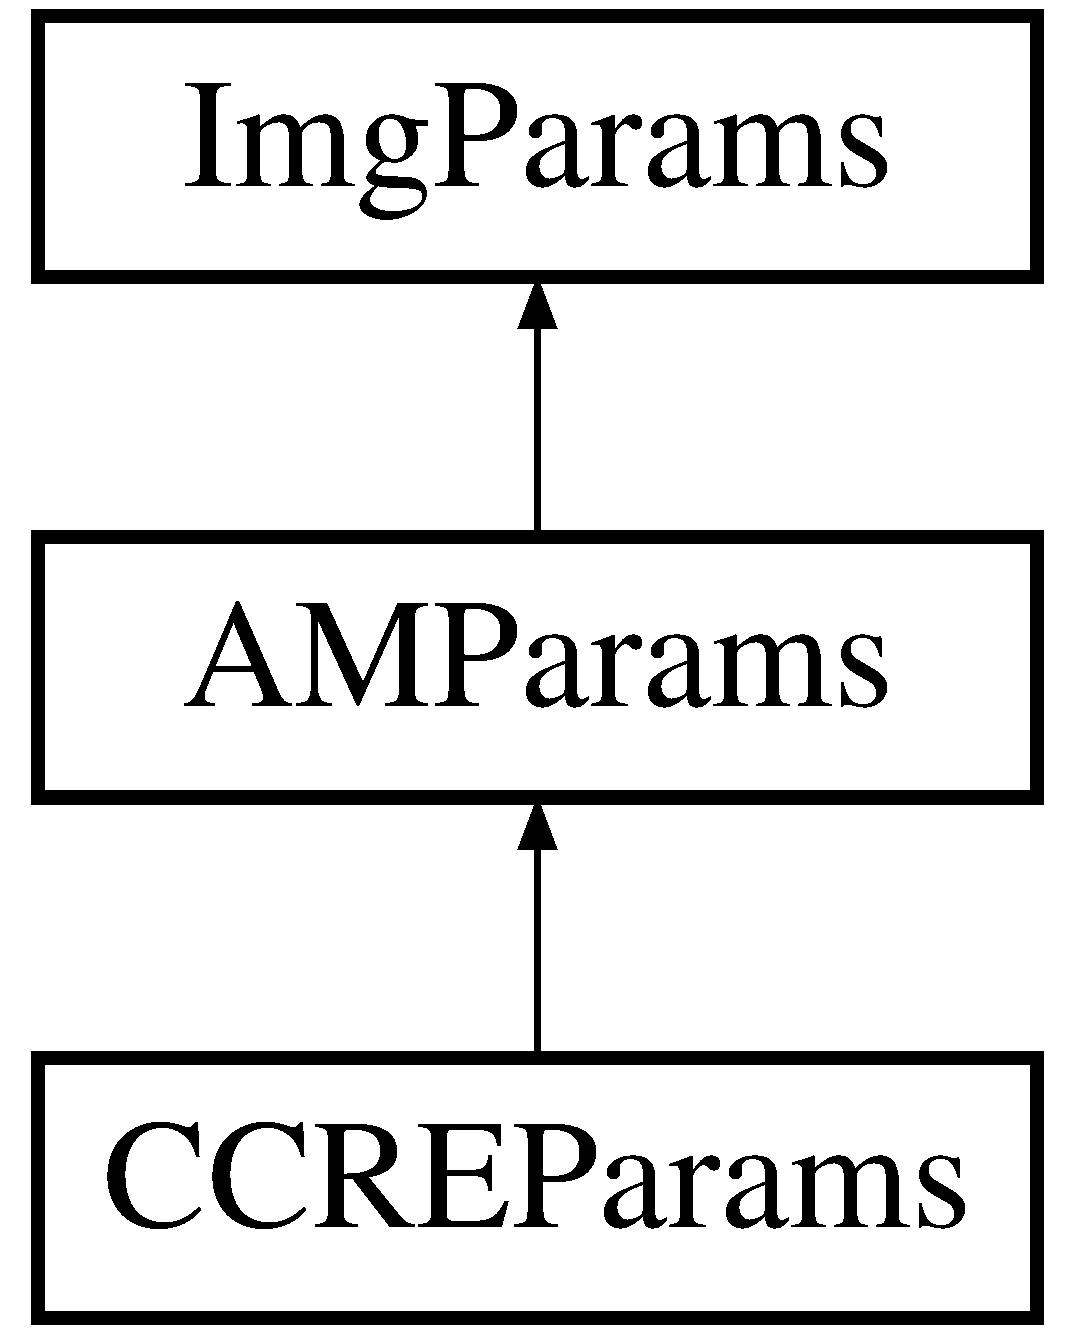
\includegraphics[height=3.000000cm]{structCCREParams}
\end{center}
\end{figure}
\subsection*{Public Member Functions}
\begin{DoxyCompactItemize}
\item 
\hypertarget{structCCREParams_ac2955cf417775818bbbe592797de0432}{\hyperlink{structCCREParams_ac2955cf417775818bbbe592797de0432}{C\-C\-R\-E\-Params} (const \hyperlink{structAMParams}{A\-M\-Params} $\ast$am\-\_\-params, int \-\_\-n\-\_\-bins, bool \-\_\-partition\-\_\-of\-\_\-unity, double \-\_\-pre\-\_\-seed, bool \-\_\-symmetrical\-\_\-grad, int \-\_\-n\-\_\-blocks, double \-\_\-likelihood\-\_\-alpha, bool \-\_\-debug\-\_\-mode)}\label{structCCREParams_ac2955cf417775818bbbe592797de0432}

\begin{DoxyCompactList}\small\item\em value constructor \end{DoxyCompactList}\item 
\hypertarget{structCCREParams_a9eebc2f5927952040ad0039b63088f9d}{\hyperlink{structCCREParams_a9eebc2f5927952040ad0039b63088f9d}{C\-C\-R\-E\-Params} (const \hyperlink{structCCREParams}{C\-C\-R\-E\-Params} $\ast$params=nullptr)}\label{structCCREParams_a9eebc2f5927952040ad0039b63088f9d}

\begin{DoxyCompactList}\small\item\em default and copy constructor \end{DoxyCompactList}\end{DoxyCompactItemize}
\subsection*{Public Attributes}
\begin{DoxyCompactItemize}
\item 
int \hyperlink{structCCREParams_afeb767eb97c56f06a0b1953a741fffa2}{n\-\_\-bins}
\begin{DoxyCompactList}\small\item\em no. \end{DoxyCompactList}\item 
\hypertarget{structCCREParams_a2846c0b115646bfe8dd61c8d43d2ee48}{bool \hyperlink{structCCREParams_a2846c0b115646bfe8dd61c8d43d2ee48}{partition\-\_\-of\-\_\-unity}}\label{structCCREParams_a2846c0b115646bfe8dd61c8d43d2ee48}

\begin{DoxyCompactList}\small\item\em decides whether the partition of unity constraint has to be strictly observed for border bins; if enabled, the pixel values will be normalized in the range \mbox{[}1, n\-\_\-bins-\/2\mbox{]} so each pixel contributes to all 4 bins \end{DoxyCompactList}\item 
double \hyperlink{structCCREParams_a17d4136ef6a1c8aae61b286531b75846}{pre\-\_\-seed}
\begin{DoxyCompactList}\small\item\em initial value with which each bin of the joint histogram is pre-\/seeded to avoid numerical instabilities due to empty or near empty bins (caused e.\-g. \end{DoxyCompactList}\item 
\hypertarget{structCCREParams_aafc4719ffd925e6db983d00f126a73f3}{bool {\bfseries symmetrical\-\_\-grad}}\label{structCCREParams_aafc4719ffd925e6db983d00f126a73f3}

\item 
\hypertarget{structCCREParams_af46b2bb4108e66d03f508cdc110603fe}{int {\bfseries n\-\_\-blocks}}\label{structCCREParams_af46b2bb4108e66d03f508cdc110603fe}

\item 
\hypertarget{structCCREParams_a554cb54ca0c4c707476e70d5c4a0f7d5}{double \hyperlink{structCCREParams_a554cb54ca0c4c707476e70d5c4a0f7d5}{likelihood\-\_\-alpha}}\label{structCCREParams_a554cb54ca0c4c707476e70d5c4a0f7d5}

\begin{DoxyCompactList}\small\item\em multiplicative factor for the exponent in the likelihood \end{DoxyCompactList}\item 
\hypertarget{structCCREParams_af07878bd091d642e47655e87f6650e1b}{bool {\bfseries debug\-\_\-mode}}\label{structCCREParams_af07878bd091d642e47655e87f6650e1b}

\end{DoxyCompactItemize}


\subsection{Member Data Documentation}
\hypertarget{structCCREParams_afeb767eb97c56f06a0b1953a741fffa2}{\index{C\-C\-R\-E\-Params@{C\-C\-R\-E\-Params}!n\-\_\-bins@{n\-\_\-bins}}
\index{n\-\_\-bins@{n\-\_\-bins}!CCREParams@{C\-C\-R\-E\-Params}}
\subsubsection[{n\-\_\-bins}]{\setlength{\rightskip}{0pt plus 5cm}int C\-C\-R\-E\-Params\-::n\-\_\-bins}}\label{structCCREParams_afeb767eb97c56f06a0b1953a741fffa2}


no. 

of bins in the histograms used internally -\/ dimensionality of the \hyperlink{classCCRE}{C\-C\-R\-E} error vector will be n\-\_\-bins $\ast$ n\-\_\-bins; if partition\-\_\-of\-\_\-unity is enabled, this should be 2 more than the desired no. of bins (w.\-r.\-t normalized pixel range) since the actual range within which the pixel values are normalized is 2 less than this value to avoid boundary conditions while computing the contribution of each pixel to different bins by ensuring that pixels with the maximum and minimum values contribute to all 4 bins required by the bspl function of degree 3 used here; \hypertarget{structCCREParams_a17d4136ef6a1c8aae61b286531b75846}{\index{C\-C\-R\-E\-Params@{C\-C\-R\-E\-Params}!pre\-\_\-seed@{pre\-\_\-seed}}
\index{pre\-\_\-seed@{pre\-\_\-seed}!CCREParams@{C\-C\-R\-E\-Params}}
\subsubsection[{pre\-\_\-seed}]{\setlength{\rightskip}{0pt plus 5cm}double C\-C\-R\-E\-Params\-::pre\-\_\-seed}}\label{structCCREParams_a17d4136ef6a1c8aae61b286531b75846}


initial value with which each bin of the joint histogram is pre-\/seeded to avoid numerical instabilities due to empty or near empty bins (caused e.\-g. 

by having to assume log(0) = 0 for empty bins) 

The documentation for this struct was generated from the following file\-:\begin{DoxyCompactItemize}
\item 
A\-M/include/mtf/\-A\-M/C\-C\-R\-E.\-h\end{DoxyCompactItemize}

\hypertarget{classCompositeBase}{\section{Composite\-Base Class Reference}
\label{classCompositeBase}\index{Composite\-Base@{Composite\-Base}}
}
Inheritance diagram for Composite\-Base\-:\begin{figure}[H]
\begin{center}
\leavevmode
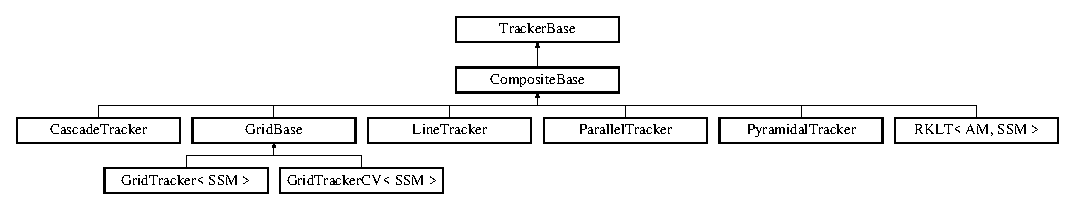
\includegraphics[height=2.377919cm]{classCompositeBase}
\end{center}
\end{figure}
\subsection*{Public Member Functions}
\begin{DoxyCompactItemize}
\item 
\hypertarget{classCompositeBase_acaaa345d5ce1c18626a5e2d2676b04bc}{{\bfseries Composite\-Base} (const vector$<$ Tracker\-Base $\ast$ $>$ \-\_\-trackers)}\label{classCompositeBase_acaaa345d5ce1c18626a5e2d2676b04bc}

\item 
\hypertarget{classCompositeBase_a9321ba237831d42c056e155cdd061a92}{void {\bfseries set\-Image} (const cv\-::\-Mat \&img) override}\label{classCompositeBase_a9321ba237831d42c056e155cdd061a92}

\item 
\hypertarget{classCompositeBase_a0466b28c23eaf6d24fca18b64f5b7460}{int {\bfseries input\-Type} () const override}\label{classCompositeBase_a0466b28c23eaf6d24fca18b64f5b7460}

\end{DoxyCompactItemize}
\subsection*{Public Attributes}
\begin{DoxyCompactItemize}
\item 
\hypertarget{classCompositeBase_a8b9f28da78a31e72a5adb8d1289b205f}{const vector$<$ Tracker\-Base $\ast$ $>$ {\bfseries trackers}}\label{classCompositeBase_a8b9f28da78a31e72a5adb8d1289b205f}

\item 
\hypertarget{classCompositeBase_a45580b3f6b80aeb5720f7ced35820da4}{int {\bfseries n\-\_\-trackers}}\label{classCompositeBase_a45580b3f6b80aeb5720f7ced35820da4}

\item 
\hypertarget{classCompositeBase_a65d083e13baa9997fc7b11cbd65d44b9}{int {\bfseries input\-\_\-type}}\label{classCompositeBase_a65d083e13baa9997fc7b11cbd65d44b9}

\end{DoxyCompactItemize}


The documentation for this class was generated from the following file\-:\begin{DoxyCompactItemize}
\item 
S\-M/include/mtf/\-S\-M/Composite\-Base.\-h\end{DoxyCompactItemize}

\hypertarget{classCompositeSM}{\section{Composite\-S\-M$<$ A\-M, S\-S\-M $>$ Class Template Reference}
\label{classCompositeSM}\index{Composite\-S\-M$<$ A\-M, S\-S\-M $>$@{Composite\-S\-M$<$ A\-M, S\-S\-M $>$}}
}


base class for all composite search methods  




{\ttfamily \#include $<$Composite\-S\-M.\-h$>$}

Inheritance diagram for Composite\-S\-M$<$ A\-M, S\-S\-M $>$\-:\begin{figure}[H]
\begin{center}
\leavevmode
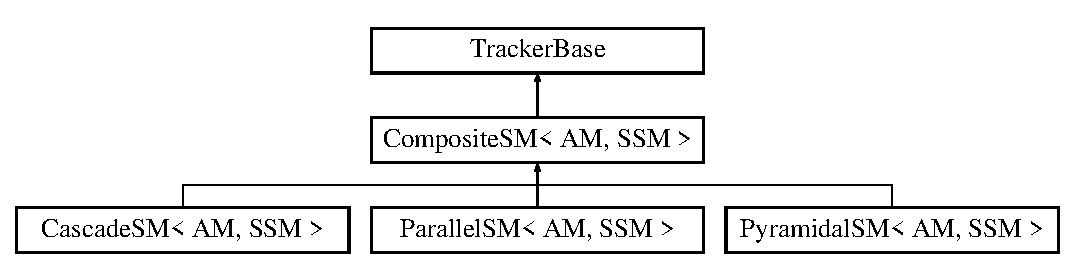
\includegraphics[height=3.000000cm]{classCompositeSM}
\end{center}
\end{figure}
\subsection*{Public Types}
\begin{DoxyCompactItemize}
\item 
\hypertarget{classCompositeSM_abf3e40ea4049c095aad36c4e0da0de43}{typedef \hyperlink{classSearchMethod}{Search\-Method}$<$ A\-M, S\-S\-M $>$ {\bfseries S\-M}}\label{classCompositeSM_abf3e40ea4049c095aad36c4e0da0de43}

\end{DoxyCompactItemize}
\subsection*{Public Member Functions}
\begin{DoxyCompactItemize}
\item 
\hyperlink{classCompositeSM_aa1d6d6e75145ebb87fb6c3ecf3134e05}{Composite\-S\-M} (const vector$<$ \hyperlink{classSearchMethod}{S\-M} $\ast$ $>$ \-\_\-trackers)
\item 
\hypertarget{classCompositeSM_a20316a95a57e6f6b75e24c4a66719a97}{void {\bfseries set\-Image} (const cv\-::\-Mat \&img) override}\label{classCompositeSM_a20316a95a57e6f6b75e24c4a66719a97}

\item 
\hypertarget{classCompositeSM_a72bc8a97252dce2bd5b541a8609bb33e}{int {\bfseries input\-Type} () const override}\label{classCompositeSM_a72bc8a97252dce2bd5b541a8609bb33e}

\item 
\hypertarget{classCompositeSM_adb512c8b6d82fbd653a48ac3d2ad9357}{void {\bfseries set\-Region} (const cv\-::\-Mat \&corners) override}\label{classCompositeSM_adb512c8b6d82fbd653a48ac3d2ad9357}

\item 
\hypertarget{classCompositeSM_ab4c4232cf45b68f31ebe25adf3d7cdb7}{virtual void {\bfseries set\-S\-P\-I\-Mask} (const bool $\ast$\-\_\-spi\-\_\-mask)}\label{classCompositeSM_ab4c4232cf45b68f31ebe25adf3d7cdb7}

\item 
\hypertarget{classCompositeSM_ab4bd7368edaaa850f75853182d733ec0}{virtual void {\bfseries clear\-S\-P\-I\-Mask} ()}\label{classCompositeSM_ab4bd7368edaaa850f75853182d733ec0}

\item 
\hypertarget{classCompositeSM_a2294250c4d7b9bbbb8b016e9bb47b683}{virtual void {\bfseries set\-Init\-Status} ()}\label{classCompositeSM_a2294250c4d7b9bbbb8b016e9bb47b683}

\item 
\hypertarget{classCompositeSM_a32a5b6531d6383909e1ef100439e8174}{virtual void {\bfseries clear\-Init\-Status} ()}\label{classCompositeSM_a32a5b6531d6383909e1ef100439e8174}

\item 
\hypertarget{classCompositeSM_aabe055e62f83356ae9fd4853410069b4}{virtual bool {\bfseries supports\-S\-P\-I} ()}\label{classCompositeSM_aabe055e62f83356ae9fd4853410069b4}

\end{DoxyCompactItemize}
\subsection*{Protected Attributes}
\begin{DoxyCompactItemize}
\item 
\hypertarget{classCompositeSM_ac60629d5d11fed646319411d9e1372aa}{const vector$<$ \hyperlink{classSearchMethod}{S\-M} $\ast$ $>$ {\bfseries trackers}}\label{classCompositeSM_ac60629d5d11fed646319411d9e1372aa}

\item 
\hypertarget{classCompositeSM_abe6f308b96f5dd274db50576cfe364d7}{int {\bfseries n\-\_\-trackers}}\label{classCompositeSM_abe6f308b96f5dd274db50576cfe364d7}

\item 
\hypertarget{classCompositeSM_aecf7653ffc7f24081acea3907d684205}{int {\bfseries input\-\_\-type}}\label{classCompositeSM_aecf7653ffc7f24081acea3907d684205}

\end{DoxyCompactItemize}


\subsection{Detailed Description}
\subsubsection*{template$<$class A\-M, class S\-S\-M$>$class Composite\-S\-M$<$ A\-M, S\-S\-M $>$}

base class for all composite search methods 

\subsection{Constructor \& Destructor Documentation}
\hypertarget{classCompositeSM_aa1d6d6e75145ebb87fb6c3ecf3134e05}{\index{Composite\-S\-M@{Composite\-S\-M}!Composite\-S\-M@{Composite\-S\-M}}
\index{Composite\-S\-M@{Composite\-S\-M}!CompositeSM@{Composite\-S\-M}}
\subsubsection[{Composite\-S\-M}]{\setlength{\rightskip}{0pt plus 5cm}template$<$class A\-M, class S\-S\-M$>$ {\bf Composite\-S\-M}$<$ A\-M, S\-S\-M $>$\-::{\bf Composite\-S\-M} (
\begin{DoxyParamCaption}
\item[{const vector$<$ {\bf S\-M} $\ast$ $>$}]{\-\_\-trackers}
\end{DoxyParamCaption}
)\hspace{0.3cm}{\ttfamily [inline]}}}\label{classCompositeSM_aa1d6d6e75145ebb87fb6c3ecf3134e05}
since all S\-Ms have the same A\-M, we can assume that they also have the same input type 

The documentation for this class was generated from the following file\-:\begin{DoxyCompactItemize}
\item 
S\-M/include/mtf/\-S\-M/Composite\-S\-M.\-h\end{DoxyCompactItemize}

\hypertarget{classCornerHomography}{\section{Corner\-Homography Class Reference}
\label{classCornerHomography}\index{Corner\-Homography@{Corner\-Homography}}
}
Inheritance diagram for Corner\-Homography\-:\begin{figure}[H]
\begin{center}
\leavevmode
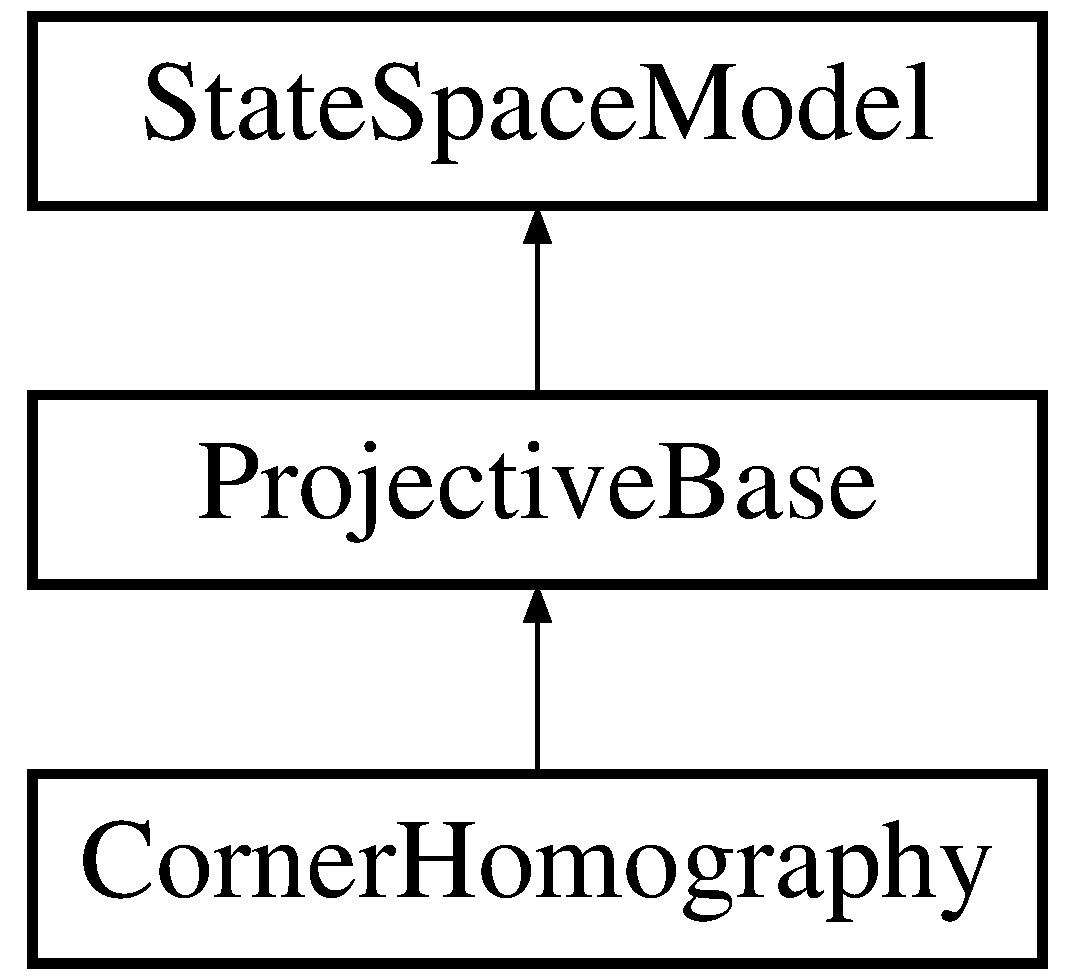
\includegraphics[height=3.000000cm]{classCornerHomography}
\end{center}
\end{figure}
\subsection*{Public Types}
\begin{DoxyCompactItemize}
\item 
\hypertarget{classCornerHomography_a1f566f572c32007c1af2227ca3db7ea8}{typedef \hyperlink{structCornerHomographyParams}{Corner\-Homography\-Params} {\bfseries Param\-Type}}\label{classCornerHomography_a1f566f572c32007c1af2227ca3db7ea8}

\end{DoxyCompactItemize}
\subsection*{Public Member Functions}
\begin{DoxyCompactItemize}
\item 
\hypertarget{classCornerHomography_a77e1e2620b3a6ed6e83135142ab6731d}{{\bfseries Corner\-Homography} (const \hyperlink{structCornerHomographyParams}{Param\-Type} $\ast$params\-\_\-in=nullptr)}\label{classCornerHomography_a77e1e2620b3a6ed6e83135142ab6731d}

\item 
\hypertarget{classCornerHomography_a187bb46c299eced70506cd62eb3e7adf}{void {\bfseries set\-Corners} (const Matrix24d \&corners) override}\label{classCornerHomography_a187bb46c299eced70506cd62eb3e7adf}

\item 
\hypertarget{classCornerHomography_a3ea82a14cfbb776cdf7d71735a8caaba}{void {\bfseries compositional\-Update} (const Vector\-Xd \&state\-\_\-update) override}\label{classCornerHomography_a3ea82a14cfbb776cdf7d71735a8caaba}

\item 
void \hyperlink{classCornerHomography_a09026e49b30f58affc5b0324747c8d1e}{cmpt\-Init\-Pix\-Jacobian} (Matrix\-Xd \&jacobian\-\_\-prod, const Pix\-Grad\-T \&am\-\_\-jacobian) override
\begin{DoxyCompactList}\small\item\em right multiplies the initial or current ssm jacobian with the provided am jacobian; though this can be accomplished by the search method itself with simple matrix multiplication, the ssm jacobian often satisfies several constraints (e.\-g. \end{DoxyCompactList}\item 
\hypertarget{classCornerHomography_adb3bf61899a9a6a907079fb9ac3823ef}{void {\bfseries cmpt\-Pix\-Jacobian} (Matrix\-Xd \&jacobian\-\_\-prod, const Pix\-Grad\-T \&am\-\_\-jacobian) override}\label{classCornerHomography_adb3bf61899a9a6a907079fb9ac3823ef}

\item 
\hypertarget{classCornerHomography_ab47607901f8e65f85ccbb5be183191f4}{void {\bfseries cmpt\-Approx\-Pix\-Jacobian} (Matrix\-Xd \&jacobian\-\_\-prod, const Pix\-Grad\-T \&pix\-\_\-jacobian) override}\label{classCornerHomography_ab47607901f8e65f85ccbb5be183191f4}

\item 
\hypertarget{classCornerHomography_a756448c9ee587e45d5804da9fc62adb6}{void {\bfseries estimate\-Warp\-From\-Corners} (Vector\-Xd \&state\-\_\-update, const Matrix24d \&in\-\_\-corners, const Matrix24d \&out\-\_\-corners) override}\label{classCornerHomography_a756448c9ee587e45d5804da9fc62adb6}

\item 
\hypertarget{classCornerHomography_a04342ba504b59adbce829cfcade2067b}{void {\bfseries estimate\-Warp\-From\-Pts} (Vector\-Xd \&state\-\_\-update, vector$<$ uchar $>$ \&mask, const vector$<$ cv\-::\-Point2f $>$ \&in\-\_\-pts, const vector$<$ cv\-::\-Point2f $>$ \&out\-\_\-pts, const \hyperlink{structSSMEstimatorParams}{Estimator\-Params} \&est\-\_\-params) override}\label{classCornerHomography_a04342ba504b59adbce829cfcade2067b}

\item 
\hypertarget{classCornerHomography_a1cb948be88d424769ed3c773dcd1dab9}{void {\bfseries invert\-State} (Vector\-Xd \&inv\-\_\-state, const Vector\-Xd \&state) override}\label{classCornerHomography_a1cb948be88d424769ed3c773dcd1dab9}

\item 
\hypertarget{classCornerHomography_a264babdc396cb341b2f3701f2fa0204b}{void {\bfseries get\-Init\-Pix\-Grad} (Matrix2\-Xd \&ssm\-\_\-grad, int pt\-\_\-id) override}\label{classCornerHomography_a264babdc396cb341b2f3701f2fa0204b}

\item 
\hypertarget{classCornerHomography_a92cc1455f29664bec0051d36e376530a}{void {\bfseries get\-Curr\-Pix\-Grad} (Matrix2\-Xd \&ssm\-\_\-grad, int pt\-\_\-id) override}\label{classCornerHomography_a92cc1455f29664bec0051d36e376530a}

\end{DoxyCompactItemize}
\subsection*{Additional Inherited Members}


\subsection{Member Function Documentation}
\hypertarget{classCornerHomography_a09026e49b30f58affc5b0324747c8d1e}{\index{Corner\-Homography@{Corner\-Homography}!cmpt\-Init\-Pix\-Jacobian@{cmpt\-Init\-Pix\-Jacobian}}
\index{cmpt\-Init\-Pix\-Jacobian@{cmpt\-Init\-Pix\-Jacobian}!CornerHomography@{Corner\-Homography}}
\subsubsection[{cmpt\-Init\-Pix\-Jacobian}]{\setlength{\rightskip}{0pt plus 5cm}void Corner\-Homography\-::cmpt\-Init\-Pix\-Jacobian (
\begin{DoxyParamCaption}
\item[{Matrix\-Xd \&}]{jacobian\-\_\-prod, }
\item[{const Pix\-Grad\-T \&}]{pixel\-\_\-grad}
\end{DoxyParamCaption}
)\hspace{0.3cm}{\ttfamily [override]}, {\ttfamily [virtual]}}}\label{classCornerHomography_a09026e49b30f58affc5b0324747c8d1e}


right multiplies the initial or current ssm jacobian with the provided am jacobian; though this can be accomplished by the search method itself with simple matrix multiplication, the ssm jacobian often satisfies several constraints (e.\-g. 

sparsity) that can be exploited to gain computational savings by manually computing the product matrix 

Reimplemented from \hyperlink{classStateSpaceModel_ac956c679581e746891c62755fe715b3b}{State\-Space\-Model}.



The documentation for this class was generated from the following file\-:\begin{DoxyCompactItemize}
\item 
S\-S\-M/include/mtf/\-S\-S\-M/Corner\-Homography.\-h\end{DoxyCompactItemize}

\hypertarget{structCornerHomographyParams}{\section{Corner\-Homography\-Params Struct Reference}
\label{structCornerHomographyParams}\index{Corner\-Homography\-Params@{Corner\-Homography\-Params}}
}
Inheritance diagram for Corner\-Homography\-Params\-:\begin{figure}[H]
\begin{center}
\leavevmode
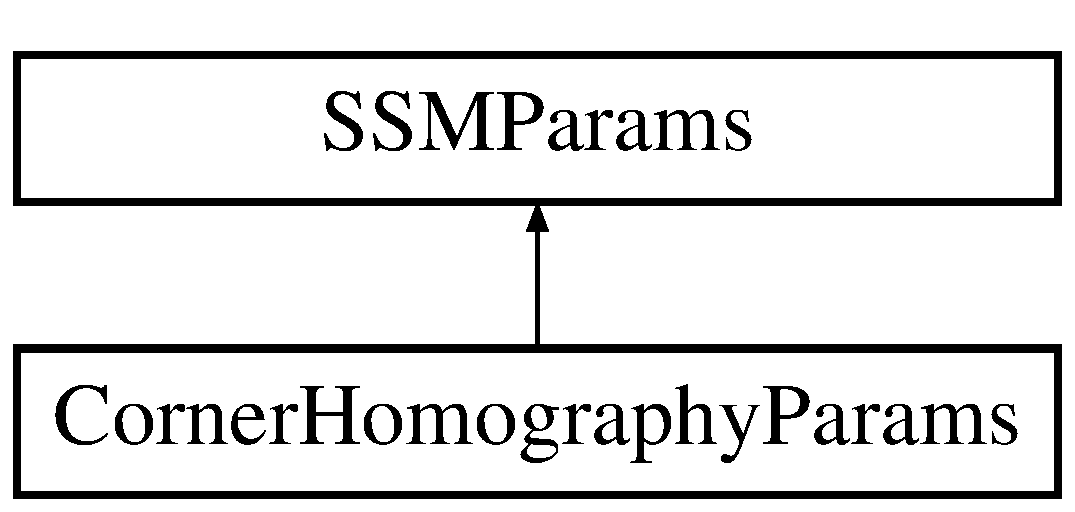
\includegraphics[height=2.000000cm]{structCornerHomographyParams}
\end{center}
\end{figure}
\subsection*{Public Member Functions}
\begin{DoxyCompactItemize}
\item 
\hypertarget{structCornerHomographyParams_ae7ee6a4557732ec5632a33fe95b6585a}{{\bfseries Corner\-Homography\-Params} (const \hyperlink{structSSMParams}{S\-S\-M\-Params} $\ast$ssm\-\_\-params, bool \-\_\-normalized\-\_\-init, double \-\_\-grad\-\_\-eps, bool \-\_\-debug\-\_\-mode)}\label{structCornerHomographyParams_ae7ee6a4557732ec5632a33fe95b6585a}

\item 
\hypertarget{structCornerHomographyParams_aa244ce18dd02613a5563d43c0e51c6d3}{{\bfseries Corner\-Homography\-Params} (const \hyperlink{structCornerHomographyParams}{Corner\-Homography\-Params} $\ast$params=nullptr)}\label{structCornerHomographyParams_aa244ce18dd02613a5563d43c0e51c6d3}

\end{DoxyCompactItemize}
\subsection*{Public Attributes}
\begin{DoxyCompactItemize}
\item 
\hypertarget{structCornerHomographyParams_a0fbf649bfcfd56cd2386a5aa9c38bc44}{bool {\bfseries normalized\-\_\-init}}\label{structCornerHomographyParams_a0fbf649bfcfd56cd2386a5aa9c38bc44}

\item 
\hypertarget{structCornerHomographyParams_ae3ddf69f1ef096caff84aa98ca55427f}{double {\bfseries grad\-\_\-eps}}\label{structCornerHomographyParams_ae3ddf69f1ef096caff84aa98ca55427f}

\item 
\hypertarget{structCornerHomographyParams_a8712cad8cb2b27ee3023d86627aaaefa}{bool {\bfseries debug\-\_\-mode}}\label{structCornerHomographyParams_a8712cad8cb2b27ee3023d86627aaaefa}

\end{DoxyCompactItemize}


The documentation for this struct was generated from the following file\-:\begin{DoxyCompactItemize}
\item 
S\-S\-M/include/mtf/\-S\-S\-M/Corner\-Homography.\-h\end{DoxyCompactItemize}

\hypertarget{classDiagBase}{\section{Diag\-Base Class Reference}
\label{classDiagBase}\index{Diag\-Base@{Diag\-Base}}
}
\subsection*{Public Types}
\begin{DoxyCompactItemize}
\item 
enum {\bfseries Analytical\-Data\-Type} \{ \\*
{\bfseries Norm}, 
{\bfseries Feat\-Norm}, 
{\bfseries Std\-Jac}, 
{\bfseries E\-S\-M\-Jac}, 
\\*
{\bfseries Diff\-Of\-Jacs}, 
{\bfseries Std}, 
{\bfseries E\-S\-M}, 
{\bfseries Init\-Self}, 
\\*
{\bfseries Curr\-Self}, 
{\bfseries Std2}, 
{\bfseries E\-S\-M2}, 
{\bfseries Init\-Self2}, 
\\*
{\bfseries Curr\-Self2}, 
{\bfseries Sum\-Of\-Std}, 
{\bfseries Sum\-Of\-Std2}, 
{\bfseries Sum\-Of\-Self}, 
\\*
{\bfseries Sum\-Of\-Self2}
 \}
\item 
enum {\bfseries Numerical\-Data\-Type} \{ {\bfseries Jacobian}, 
{\bfseries Hessian}, 
{\bfseries N\-Hessian}
 \}
\item 
\hypertarget{classDiagBase_a426a116745989c7137fb512fa7d584f2}{typedef Analytical\-Data\-Type {\bfseries A\-D\-T}}\label{classDiagBase_a426a116745989c7137fb512fa7d584f2}

\item 
\hypertarget{classDiagBase_a5ec839186aabccb0f15827bfa3b5642e}{typedef Numerical\-Data\-Type {\bfseries N\-D\-T}}\label{classDiagBase_a5ec839186aabccb0f15827bfa3b5642e}

\end{DoxyCompactItemize}
\subsection*{Public Member Functions}
\begin{DoxyCompactItemize}
\item 
\hypertarget{classDiagBase_a0f5852709cb03bc86b5fca81f0483325}{{\bfseries Diag\-Base} (const cv\-::\-Mat \&init\-\_\-img)}\label{classDiagBase_a0f5852709cb03bc86b5fca81f0483325}

\item 
\hypertarget{classDiagBase_ab26161b77dd7a9161f8945f761feb61c}{virtual void {\bfseries set\-Image} (const cv\-::\-Mat \&img)=0}\label{classDiagBase_ab26161b77dd7a9161f8945f761feb61c}

\item 
\hypertarget{classDiagBase_a3a1cf2490a7647027c0f86e80c43bb03}{virtual void {\bfseries initialize} (const cv\-::\-Mat \&corners)=0}\label{classDiagBase_a3a1cf2490a7647027c0f86e80c43bb03}

\item 
\hypertarget{classDiagBase_ae1eb9474a09592e6daf0f0a776bf678f}{virtual void {\bfseries update} (const cv\-::\-Mat \&corners)=0}\label{classDiagBase_ae1eb9474a09592e6daf0f0a776bf678f}

\item 
\hypertarget{classDiagBase_acd4b15bf4f6bf3d3092f0a66e781127b}{virtual void {\bfseries initialize} (const cv\-::\-Mat \&img, const cv\-::\-Mat \&corners)}\label{classDiagBase_acd4b15bf4f6bf3d3092f0a66e781127b}

\item 
\hypertarget{classDiagBase_a1dda6929b6f96ce23581a379ad9c2d59}{virtual void {\bfseries update} (const cv\-::\-Mat \&img, const cv\-::\-Mat \&corners)}\label{classDiagBase_a1dda6929b6f96ce23581a379ad9c2d59}

\item 
\hypertarget{classDiagBase_a2ec31e3a577a7f2388b4dfaf5e1ed899}{virtual void {\bfseries generate\-Analytical\-Data} (Vector\-Xd \&param\-\_\-range, int n\-\_\-pts, Analytical\-Data\-Type data\-\_\-type, const char $\ast$fname)=0}\label{classDiagBase_a2ec31e3a577a7f2388b4dfaf5e1ed899}

\item 
\hypertarget{classDiagBase_a663aa4697855857c281ead3acdc2c04d}{void {\bfseries generate\-Analytical\-Data} (double param\-\_\-range, int n\-\_\-pts, Analytical\-Data\-Type data\-\_\-type, const char $\ast$fname=nullptr)}\label{classDiagBase_a663aa4697855857c281ead3acdc2c04d}

\item 
\hypertarget{classDiagBase_a3750265ecae09e3f48b441475560bd20}{virtual void {\bfseries generate\-Inverse\-Analytical\-Data} (Vector\-Xd \&param\-\_\-range, int n\-\_\-pts, Analytical\-Data\-Type data\-\_\-type, const char $\ast$fname=nullptr)=0}\label{classDiagBase_a3750265ecae09e3f48b441475560bd20}

\item 
\hypertarget{classDiagBase_ad8b6f94744ede59ee7138f6b1864d399}{void {\bfseries generate\-Inverse\-Analytical\-Data} (double param\-\_\-range, int n\-\_\-pts, Analytical\-Data\-Type data\-\_\-type, const char $\ast$fname=nullptr)}\label{classDiagBase_ad8b6f94744ede59ee7138f6b1864d399}

\item 
\hypertarget{classDiagBase_ad0fe63d853e3a68c05238c387fa4e9e7}{virtual void {\bfseries generate\-Numerical\-Data} (Vector\-Xd \&param\-\_\-range\-\_\-vec, int n\-\_\-pts, Numerical\-Data\-Type data\-\_\-type, const char $\ast$fname, double grad\-\_\-diff)=0}\label{classDiagBase_ad0fe63d853e3a68c05238c387fa4e9e7}

\item 
\hypertarget{classDiagBase_a1ced10e03d9d0c18ce9a7552f819f03b}{virtual void {\bfseries generate\-Inverse\-Numerical\-Data} (Vector\-Xd \&param\-\_\-range\-\_\-vec, int n\-\_\-pts, Numerical\-Data\-Type data\-\_\-type, const char $\ast$fname, double grad\-\_\-diff)=0}\label{classDiagBase_a1ced10e03d9d0c18ce9a7552f819f03b}

\item 
\hypertarget{classDiagBase_a44290bbaff4edc2862e6a6b14791118a}{virtual void {\bfseries generate\-S\-S\-M\-Param\-Data} (Vector\-Xd \&param\-\_\-range\-\_\-vec, int n\-\_\-pts, const char $\ast$fname)=0}\label{classDiagBase_a44290bbaff4edc2862e6a6b14791118a}

\item 
\hypertarget{classDiagBase_a0d84250f6110072f3ca9dbff0cd6e04c}{const char $\ast$ {\bfseries to\-String} (Analytical\-Data\-Type data\-\_\-type)}\label{classDiagBase_a0d84250f6110072f3ca9dbff0cd6e04c}

\item 
\hypertarget{classDiagBase_ad416e2fbded87de6c9752fcccd71fca3}{const char $\ast$ {\bfseries to\-String} (Numerical\-Data\-Type data\-\_\-type)}\label{classDiagBase_ad416e2fbded87de6c9752fcccd71fca3}

\end{DoxyCompactItemize}
\subsection*{Public Attributes}
\begin{DoxyCompactItemize}
\item 
\hypertarget{classDiagBase_ad4d3d755e60652be0c047aa53b2467ef}{int {\bfseries am\-\_\-dist\-\_\-size}}\label{classDiagBase_ad4d3d755e60652be0c047aa53b2467ef}

\item 
\hypertarget{classDiagBase_a616730726a2503ca6f2aaeebe403289f}{int {\bfseries ssm\-\_\-state\-\_\-size}}\label{classDiagBase_a616730726a2503ca6f2aaeebe403289f}

\item 
\hypertarget{classDiagBase_a8f6e96646d472f0f46612d95a263dd93}{Matrix\-Xd {\bfseries diagnostics\-\_\-data}}\label{classDiagBase_a8f6e96646d472f0f46612d95a263dd93}

\end{DoxyCompactItemize}


The documentation for this class was generated from the following file\-:\begin{DoxyCompactItemize}
\item 
Test/include/mtf/\-Test/Diag\-Base.\-h\end{DoxyCompactItemize}

\hypertarget{classDiagnostics}{\section{Diagnostics Class Reference}
\label{classDiagnostics}\index{Diagnostics@{Diagnostics}}
}
\subsection*{Public Types}
\begin{DoxyCompactItemize}
\item 
enum {\bfseries Analytical\-Data\-Type} \{ \\*
{\bfseries Norm}, 
{\bfseries Feat\-Norm}, 
{\bfseries Likelihood}, 
{\bfseries Std\-Jac}, 
\\*
{\bfseries E\-S\-M\-Jac}, 
{\bfseries Diff\-Of\-Jacs}, 
{\bfseries Std}, 
{\bfseries E\-S\-M}, 
\\*
{\bfseries Init\-Self}, 
{\bfseries Curr\-Self}, 
{\bfseries Std2}, 
{\bfseries E\-S\-M2}, 
\\*
{\bfseries Init\-Self2}, 
{\bfseries Curr\-Self2}, 
{\bfseries Sum\-Of\-Std}, 
{\bfseries Sum\-Of\-Std2}, 
\\*
{\bfseries Sum\-Of\-Self}, 
{\bfseries Sum\-Of\-Self2}
 \}
\item 
enum {\bfseries Numerical\-Data\-Type} \{ {\bfseries Jacobian}, 
{\bfseries Hessian}, 
{\bfseries N\-Hessian}
 \}
\item 
\hypertarget{classDiagnostics_aaa74367def8ecd47fb74ed8139fdb597}{typedef \hyperlink{structDiagnosticsParams}{Diagnostics\-Params} {\bfseries Param\-Type}}\label{classDiagnostics_aaa74367def8ecd47fb74ed8139fdb597}

\item 
\hypertarget{classDiagnostics_a799ea9a90dd339554076d5b75a4a729b}{typedef \hyperlink{classAppearanceModel}{Appearance\-Model} {\bfseries A\-M}}\label{classDiagnostics_a799ea9a90dd339554076d5b75a4a729b}

\item 
\hypertarget{classDiagnostics_a60b812b16f0ec8d07415a767b4ca4c13}{typedef \hyperlink{classStateSpaceModel}{State\-Space\-Model} {\bfseries S\-S\-M}}\label{classDiagnostics_a60b812b16f0ec8d07415a767b4ca4c13}

\item 
\hypertarget{classDiagnostics_ab119ce19e765c876b51813134d41472a}{typedef Analytical\-Data\-Type {\bfseries A\-D\-T}}\label{classDiagnostics_ab119ce19e765c876b51813134d41472a}

\item 
\hypertarget{classDiagnostics_a1c065aa9240fa0b6c2a969f50e4300ef}{typedef Numerical\-Data\-Type {\bfseries N\-D\-T}}\label{classDiagnostics_a1c065aa9240fa0b6c2a969f50e4300ef}

\item 
\hypertarget{classDiagnostics_af33d67ba361be1ef33213b92aadd7110}{typedef Param\-Type\-::\-Update\-Type {\bfseries Update\-Type}}\label{classDiagnostics_af33d67ba361be1ef33213b92aadd7110}

\end{DoxyCompactItemize}
\subsection*{Public Member Functions}
\begin{DoxyCompactItemize}
\item 
\hypertarget{classDiagnostics_a0a57a2e983c529eb2113a537101a932d}{const Matrix\-Xd \& {\bfseries get\-Data} ()}\label{classDiagnostics_a0a57a2e983c529eb2113a537101a932d}

\item 
\hypertarget{classDiagnostics_abd2d8842d4f8ac0ceac08a95aa3859d1}{{\bfseries Diagnostics} (\hyperlink{classAppearanceModel}{A\-M} $\ast$\-\_\-am, \hyperlink{classStateSpaceModel}{S\-S\-M} $\ast$\-\_\-ssm, const \hyperlink{structDiagnosticsParams}{Param\-Type} $\ast$diag\-\_\-params=nullptr)}\label{classDiagnostics_abd2d8842d4f8ac0ceac08a95aa3859d1}

\item 
\hypertarget{classDiagnostics_a14df56879f2201ac635cdfd78f83007f}{int {\bfseries input\-Type} () const }\label{classDiagnostics_a14df56879f2201ac635cdfd78f83007f}

\item 
\hypertarget{classDiagnostics_a41e939e1d3f1928bb1b4f9b8b0082f1f}{void {\bfseries set\-Image} (const cv\-::\-Mat \&img)}\label{classDiagnostics_a41e939e1d3f1928bb1b4f9b8b0082f1f}

\item 
\hypertarget{classDiagnostics_a995b4956646986d22a3d9ae943e126bc}{void {\bfseries initialize} (const cv\-::\-Mat \&corners)}\label{classDiagnostics_a995b4956646986d22a3d9ae943e126bc}

\item 
\hypertarget{classDiagnostics_a534f0a7cb24b2593f3a6bcb646e33199}{void {\bfseries update} (const cv\-::\-Mat \&corners)}\label{classDiagnostics_a534f0a7cb24b2593f3a6bcb646e33199}

\item 
\hypertarget{classDiagnostics_afb2b5c2cbc835a92aca06726e0a881bb}{void {\bfseries generate\-Analytical\-Data} (Vector\-Xd \&param\-\_\-range, int n\-\_\-pts, A\-D\-T data\-\_\-type, const char $\ast$fname=nullptr)}\label{classDiagnostics_afb2b5c2cbc835a92aca06726e0a881bb}

\item 
\hypertarget{classDiagnostics_afad7cb1263188f6430f352a82c830b6c}{void {\bfseries generate\-Analytical\-Data3\-D} (Vector\-Xd \&x\-\_\-vec, Vector\-Xd \&y\-\_\-vec, const Vector\-Xd \&param\-\_\-range, int n\-\_\-pts, const Vector2d \&state\-\_\-ids, A\-D\-T data\-\_\-type, const char $\ast$fname=nullptr)}\label{classDiagnostics_afad7cb1263188f6430f352a82c830b6c}

\item 
\hypertarget{classDiagnostics_a8a57ff04d757f8a636c39612f662fa84}{void {\bfseries generate\-Inverse\-Analytical\-Data} (Vector\-Xd \&param\-\_\-range, int n\-\_\-pts, A\-D\-T data\-\_\-type, const char $\ast$fname=nullptr)}\label{classDiagnostics_a8a57ff04d757f8a636c39612f662fa84}

\item 
\hypertarget{classDiagnostics_ad0ad6ffb5f002e0e8a1ecc338448d110}{void {\bfseries generate\-Numerical\-Data} (Vector\-Xd \&param\-\_\-range\-\_\-vec, int n\-\_\-pts, N\-D\-T data\-\_\-type, const char $\ast$fname, double grad\-\_\-diff)}\label{classDiagnostics_ad0ad6ffb5f002e0e8a1ecc338448d110}

\item 
\hypertarget{classDiagnostics_a9abeba172d4abb8eb7c0af244db62f2b}{void {\bfseries generate\-Inverse\-Numerical\-Data} (Vector\-Xd \&param\-\_\-range\-\_\-vec, int n\-\_\-pts, N\-D\-T data\-\_\-type, const char $\ast$fname, double grad\-\_\-diff)}\label{classDiagnostics_a9abeba172d4abb8eb7c0af244db62f2b}

\item 
\hypertarget{classDiagnostics_a2bb91e6c3834e78bd9c942dafd4bbd2d}{void {\bfseries generate\-S\-S\-M\-Param\-Data} (Vector\-Xd \&param\-\_\-range\-\_\-vec, int n\-\_\-pts, const char $\ast$fname)}\label{classDiagnostics_a2bb91e6c3834e78bd9c942dafd4bbd2d}

\item 
\hypertarget{classDiagnostics_add36dde58c8394f3f8114917dff0a6d2}{double {\bfseries get\-A\-D\-T\-Val} (A\-D\-T data\-\_\-type, int state\-\_\-id)}\label{classDiagnostics_add36dde58c8394f3f8114917dff0a6d2}

\item 
\hypertarget{classDiagnostics_afb08d86a96a43318682d79b51b366d69}{const char $\ast$ {\bfseries to\-String} (A\-D\-T data\-\_\-type)}\label{classDiagnostics_afb08d86a96a43318682d79b51b366d69}

\item 
\hypertarget{classDiagnostics_a5e41fad93ecbd3fe6f91fa2f3d2e7c40}{const char $\ast$ {\bfseries to\-String} (N\-D\-T data\-\_\-type)}\label{classDiagnostics_a5e41fad93ecbd3fe6f91fa2f3d2e7c40}

\end{DoxyCompactItemize}
\subsection*{Public Attributes}
\begin{DoxyCompactItemize}
\item 
\hypertarget{classDiagnostics_a1200b9152d409c31a3cf7b7330284d8e}{\hyperlink{structDiagnosticsParams}{Param\-Type} {\bfseries params}}\label{classDiagnostics_a1200b9152d409c31a3cf7b7330284d8e}

\item 
\hypertarget{classDiagnostics_a2a435594e85958655964372f3e740133}{int {\bfseries am\-\_\-dist\-\_\-size}}\label{classDiagnostics_a2a435594e85958655964372f3e740133}

\item 
\hypertarget{classDiagnostics_a97200fc956e8e95b33998a49e28d9fc4}{int {\bfseries ssm\-\_\-state\-\_\-size}}\label{classDiagnostics_a97200fc956e8e95b33998a49e28d9fc4}

\item 
\hypertarget{classDiagnostics_a3f234df63a32fa05e3104625db896619}{\hyperlink{classAppearanceModel}{A\-M} $\ast$ {\bfseries am}}\label{classDiagnostics_a3f234df63a32fa05e3104625db896619}

\item 
\hypertarget{classDiagnostics_a0a8a0aedaf934678e11fa7e13ece6268}{\hyperlink{classStateSpaceModel}{S\-S\-M} $\ast$ {\bfseries ssm}}\label{classDiagnostics_a0a8a0aedaf934678e11fa7e13ece6268}

\item 
\hypertarget{classDiagnostics_aae4dcb5c6976107eb93db5b70700ad4c}{int {\bfseries frame\-\_\-id}}\label{classDiagnostics_aae4dcb5c6976107eb93db5b70700ad4c}

\item 
\hypertarget{classDiagnostics_a9290ee9650cc84ac5724bd1bb6dbca3c}{int {\bfseries n\-\_\-pix}}\label{classDiagnostics_a9290ee9650cc84ac5724bd1bb6dbca3c}

\item 
\hypertarget{classDiagnostics_ae8f2058e10d18570654bfb62d2ce4bfe}{Vector\-Xd {\bfseries inv\-\_\-state}}\label{classDiagnostics_ae8f2058e10d18570654bfb62d2ce4bfe}

\item 
Matrix\-Xd \hyperlink{classDiagnostics_a1a89abf10430a264cd699d0f4f199fd2}{init\-\_\-pix\-\_\-jacobian}
\begin{DoxyCompactList}\small\item\em N x S jacobians of the pix values w.\-r.\-t the S\-S\-M state vector where N = resx $\ast$ resy is the no. \end{DoxyCompactList}\item 
\hypertarget{classDiagnostics_a006cbd7a6a2d3cd1dc1fc071dbfe1c8d}{Matrix\-Xd {\bfseries init\-\_\-pix\-\_\-hessian}}\label{classDiagnostics_a006cbd7a6a2d3cd1dc1fc071dbfe1c8d}

\item 
\hypertarget{classDiagnostics_aa0d81d679032bd5ec54504806c3b3b65}{Matrix\-Xd {\bfseries curr\-\_\-pix\-\_\-jacobian}}\label{classDiagnostics_aa0d81d679032bd5ec54504806c3b3b65}

\item 
\hypertarget{classDiagnostics_a93756de17709a056f143941c9c9633c1}{Matrix\-Xd {\bfseries curr\-\_\-pix\-\_\-hessian}}\label{classDiagnostics_a93756de17709a056f143941c9c9633c1}

\item 
\hypertarget{classDiagnostics_ae111d0a62eb53ff3d22b4e4244104da5}{Matrix\-Xd {\bfseries mean\-\_\-pix\-\_\-jacobian}}\label{classDiagnostics_ae111d0a62eb53ff3d22b4e4244104da5}

\item 
\hypertarget{classDiagnostics_a5d6ec9a29a3633af3191f8535258e63e}{Matrix\-Xd {\bfseries mean\-\_\-pix\-\_\-hessian}}\label{classDiagnostics_a5d6ec9a29a3633af3191f8535258e63e}

\item 
\hypertarget{classDiagnostics_a0c912c49fc34a709e92ef6567718c55c}{Row\-Vector\-Xd \hyperlink{classDiagnostics_a0c912c49fc34a709e92ef6567718c55c}{similarity\-\_\-jacobian}}\label{classDiagnostics_a0c912c49fc34a709e92ef6567718c55c}

\begin{DoxyCompactList}\small\item\em 1 x S Jacobian of the A\-M error norm w.\-r.\-t. S\-S\-M state vector \end{DoxyCompactList}\item 
\hypertarget{classDiagnostics_a7ed879e92b97e12309bb1e3600cf85d9}{Matrix\-Xd \hyperlink{classDiagnostics_a7ed879e92b97e12309bb1e3600cf85d9}{hessian}}\label{classDiagnostics_a7ed879e92b97e12309bb1e3600cf85d9}

\begin{DoxyCompactList}\small\item\em S x S Hessian of the A\-M error norm w.\-r.\-t. S\-S\-M state vector. \end{DoxyCompactList}\item 
\hypertarget{classDiagnostics_a81b44beee4337cf75dfb1a2a57435695}{Matrix\-Xd {\bfseries init\-\_\-hessian}}\label{classDiagnostics_a81b44beee4337cf75dfb1a2a57435695}

\item 
\hypertarget{classDiagnostics_aa514bd591c607d57586fff54867be0bc}{Matrix\-Xd {\bfseries init\-\_\-self\-\_\-hessian}}\label{classDiagnostics_aa514bd591c607d57586fff54867be0bc}

\item 
\hypertarget{classDiagnostics_ac426c9c540ac32ff721da5c6b979b419}{Matrix\-Xd {\bfseries init\-\_\-self\-\_\-hessian2}}\label{classDiagnostics_ac426c9c540ac32ff721da5c6b979b419}

\item 
\hypertarget{classDiagnostics_ac4ee422a13848bdcf678af0337ac64b3}{Matrix\-Xd {\bfseries curr\-\_\-self\-\_\-hessian}}\label{classDiagnostics_ac4ee422a13848bdcf678af0337ac64b3}

\item 
\hypertarget{classDiagnostics_abaa5455c6d26b4ec15e774b28f95dcd0}{Matrix\-Xd {\bfseries curr\-\_\-self\-\_\-hessian2}}\label{classDiagnostics_abaa5455c6d26b4ec15e774b28f95dcd0}

\item 
\hypertarget{classDiagnostics_a2af3fb7574813574f5cec2215469cd01}{Vector\-Xd {\bfseries init\-\_\-dist\-\_\-vec}}\label{classDiagnostics_a2af3fb7574813574f5cec2215469cd01}

\item 
\hypertarget{classDiagnostics_aeb0d7308c472a2319b0e2390e90879a8}{Vector\-Xd {\bfseries curr\-\_\-dist\-\_\-vec}}\label{classDiagnostics_aeb0d7308c472a2319b0e2390e90879a8}

\item 
\hypertarget{classDiagnostics_a749cd007342b2086f3fff83e70086d59}{Matrix3d {\bfseries warp\-\_\-update}}\label{classDiagnostics_a749cd007342b2086f3fff83e70086d59}

\item 
\hypertarget{classDiagnostics_a9630a4d0e76ba39701877fb6ebcb533a}{char $\ast$ {\bfseries update\-\_\-name}}\label{classDiagnostics_a9630a4d0e76ba39701877fb6ebcb533a}

\end{DoxyCompactItemize}


\subsection{Member Data Documentation}
\hypertarget{classDiagnostics_a1a89abf10430a264cd699d0f4f199fd2}{\index{Diagnostics@{Diagnostics}!init\-\_\-pix\-\_\-jacobian@{init\-\_\-pix\-\_\-jacobian}}
\index{init\-\_\-pix\-\_\-jacobian@{init\-\_\-pix\-\_\-jacobian}!Diagnostics@{Diagnostics}}
\subsubsection[{init\-\_\-pix\-\_\-jacobian}]{\setlength{\rightskip}{0pt plus 5cm}Matrix\-Xd Diagnostics\-::init\-\_\-pix\-\_\-jacobian}}\label{classDiagnostics_a1a89abf10430a264cd699d0f4f199fd2}


N x S jacobians of the pix values w.\-r.\-t the S\-S\-M state vector where N = resx $\ast$ resy is the no. 

of pixels in the object patch 

The documentation for this class was generated from the following file\-:\begin{DoxyCompactItemize}
\item 
Test/include/mtf/\-Test/Diagnostics.\-h\end{DoxyCompactItemize}

\hypertarget{structDiagnosticsParams}{\section{Diagnostics\-Params Struct Reference}
\label{structDiagnosticsParams}\index{Diagnostics\-Params@{Diagnostics\-Params}}
}
\subsection*{Public Types}
\begin{DoxyCompactItemize}
\item 
enum {\bfseries Update\-Type} \{ {\bfseries Additive}, 
{\bfseries Compositional}
 \}
\end{DoxyCompactItemize}
\subsection*{Public Member Functions}
\begin{DoxyCompactItemize}
\item 
\hypertarget{structDiagnosticsParams_ab36a7e885f3961c0469b5f53f0cc1203}{{\bfseries Diagnostics\-Params} (Update\-Type \-\_\-update\-\_\-type, bool \-\_\-show\-\_\-corners, bool \-\_\-show\-\_\-patches, bool \-\_\-enable\-\_\-validation, double \-\_\-validation\-\_\-prec)}\label{structDiagnosticsParams_ab36a7e885f3961c0469b5f53f0cc1203}

\item 
\hypertarget{structDiagnosticsParams_a41a0eda527e1e2e523dced1f3820b2e8}{{\bfseries Diagnostics\-Params} (const \hyperlink{structDiagnosticsParams}{Diagnostics\-Params} $\ast$params=nullptr)}\label{structDiagnosticsParams_a41a0eda527e1e2e523dced1f3820b2e8}

\end{DoxyCompactItemize}
\subsection*{Public Attributes}
\begin{DoxyCompactItemize}
\item 
\hypertarget{structDiagnosticsParams_aefd23c8724dece8438b29f364c3ab2e0}{Update\-Type {\bfseries update\-\_\-type}}\label{structDiagnosticsParams_aefd23c8724dece8438b29f364c3ab2e0}

\item 
\hypertarget{structDiagnosticsParams_afe4101321aff7562698e879000db7999}{bool {\bfseries show\-\_\-corners}}\label{structDiagnosticsParams_afe4101321aff7562698e879000db7999}

\item 
\hypertarget{structDiagnosticsParams_ad761a87f2aaed018701ff35b17270135}{bool {\bfseries show\-\_\-patches}}\label{structDiagnosticsParams_ad761a87f2aaed018701ff35b17270135}

\item 
\hypertarget{structDiagnosticsParams_ae32e84a44638a5ad5c01737f208ff139}{bool {\bfseries enable\-\_\-validation}}\label{structDiagnosticsParams_ae32e84a44638a5ad5c01737f208ff139}

\item 
\hypertarget{structDiagnosticsParams_a5852e14acd13967278975a54b8bb8cb5}{double {\bfseries validation\-\_\-prec}}\label{structDiagnosticsParams_a5852e14acd13967278975a54b8bb8cb5}

\end{DoxyCompactItemize}


The documentation for this struct was generated from the following file\-:\begin{DoxyCompactItemize}
\item 
Test/include/mtf/\-Test/Diagnostics.\-h\end{DoxyCompactItemize}

\hypertarget{classESM}{\section{E\-S\-M$<$ A\-M, S\-S\-M $>$ Class Template Reference}
\label{classESM}\index{E\-S\-M$<$ A\-M, S\-S\-M $>$@{E\-S\-M$<$ A\-M, S\-S\-M $>$}}
}
Inheritance diagram for E\-S\-M$<$ A\-M, S\-S\-M $>$\-:\begin{figure}[H]
\begin{center}
\leavevmode
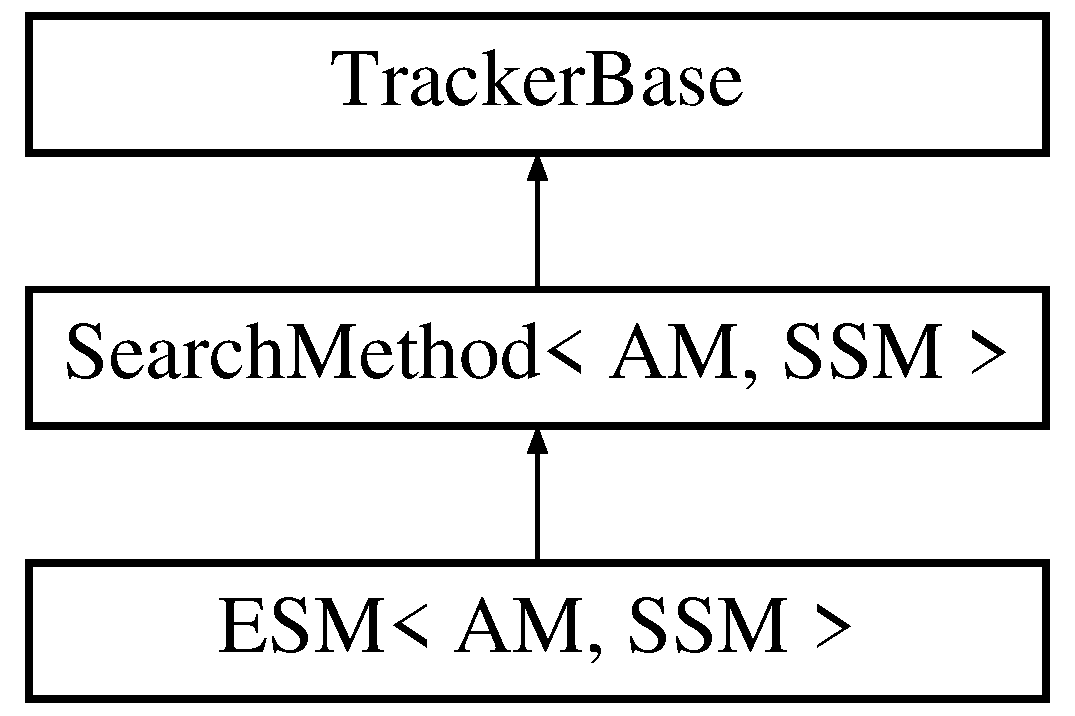
\includegraphics[height=3.000000cm]{classESM}
\end{center}
\end{figure}
\subsection*{Public Types}
\begin{DoxyCompactItemize}
\item 
\hypertarget{classESM_a30b6609c9b894182e6fab15d725fe64c}{typedef \hyperlink{structESMParams}{E\-S\-M\-Params} {\bfseries Param\-Type}}\label{classESM_a30b6609c9b894182e6fab15d725fe64c}

\item 
\hypertarget{classESM_a4d4d5b39b63a16173d4b50d0a811195b}{typedef Param\-Type\-::\-Jac\-Type {\bfseries Jac\-Type}}\label{classESM_a4d4d5b39b63a16173d4b50d0a811195b}

\item 
\hypertarget{classESM_a3f8ad5f74ac439f7c2681143d5b6507b}{typedef Param\-Type\-::\-Hess\-Type {\bfseries Hess\-Type}}\label{classESM_a3f8ad5f74ac439f7c2681143d5b6507b}

\end{DoxyCompactItemize}
\subsection*{Public Member Functions}
\begin{DoxyCompactItemize}
\item 
\hypertarget{classESM_ac953fa7deaee7a9264372f6dcba44a66}{{\bfseries E\-S\-M} (const \hyperlink{structESMParams}{Param\-Type} $\ast$esm\-\_\-params=nullptr, const \hyperlink{structAMParams}{A\-M\-Params} $\ast$am\-\_\-params=nullptr, const \hyperlink{structSSMParams}{S\-S\-M\-Params} $\ast$ssm\-\_\-params=nullptr)}\label{classESM_ac953fa7deaee7a9264372f6dcba44a66}

\item 
\hypertarget{classESM_ae5ec5d4f28ae33d4a2080096c2f8482c}{void {\bfseries initialize} (const cv\-::\-Mat \&corners) override}\label{classESM_ae5ec5d4f28ae33d4a2080096c2f8482c}

\item 
\hypertarget{classESM_a43a8457c148f57a0d56b3f857efb60ce}{void {\bfseries update} () override}\label{classESM_a43a8457c148f57a0d56b3f857efb60ce}

\item 
\hypertarget{classESM_a43390c8a9b71b7fac668519e56371aa5}{void {\bfseries set\-Region} (const cv\-::\-Mat \&corners) override}\label{classESM_a43390c8a9b71b7fac668519e56371aa5}

\end{DoxyCompactItemize}
\subsection*{Public Attributes}
\begin{DoxyCompactItemize}
\item 
\hypertarget{classESM_ad4dd514e166aff60c889b194d7126025}{\hyperlink{structESMParams}{Param\-Type} {\bfseries params}}\label{classESM_ad4dd514e166aff60c889b194d7126025}

\end{DoxyCompactItemize}
\subsection*{Protected Member Functions}
\begin{DoxyCompactItemize}
\item 
\hypertarget{classESM_a94615f6ec2c83d02b2479a6350906ee4}{{\bfseries init\-\_\-profiling} ()}\label{classESM_a94615f6ec2c83d02b2479a6350906ee4}

\end{DoxyCompactItemize}
\subsection*{Protected Attributes}
\begin{DoxyCompactItemize}
\item 
\hypertarget{classESM_adf2dd5b5bd4503409811737ca7fc2da9}{int {\bfseries frame\-\_\-id}}\label{classESM_adf2dd5b5bd4503409811737ca7fc2da9}

\item 
\hypertarget{classESM_a2f4ea2877a533a8f8baea61c68534604}{Matrix24d {\bfseries prev\-\_\-corners}}\label{classESM_a2f4ea2877a533a8f8baea61c68534604}

\item 
Matrix\-Xd \hyperlink{classESM_a94ba04c1951052b8d82377aff8aab97c}{init\-\_\-pix\-\_\-jacobian}
\begin{DoxyCompactList}\small\item\em N x S jacobians of the pixel values w.\-r.\-t the S\-S\-M state vector where N = resx $\ast$ resy is the no. \end{DoxyCompactList}\item 
\hypertarget{classESM_a3ffe05e2d3bb4bf5a35f74072c0b1d75}{Matrix\-Xd {\bfseries curr\-\_\-pix\-\_\-jacobian}}\label{classESM_a3ffe05e2d3bb4bf5a35f74072c0b1d75}

\item 
\hypertarget{classESM_a89876e6e8f509aa15ded3268198ea41a}{Matrix\-Xd {\bfseries mean\-\_\-pix\-\_\-jacobian}}\label{classESM_a89876e6e8f509aa15ded3268198ea41a}

\item 
\hypertarget{classESM_ae81ed47c90e85af190d2903a3134e413}{Matrix\-Xd {\bfseries init\-\_\-pix\-\_\-hessian}}\label{classESM_ae81ed47c90e85af190d2903a3134e413}

\item 
\hypertarget{classESM_a0e887fb0aca62133e62424698c3b1a57}{Matrix\-Xd {\bfseries curr\-\_\-pix\-\_\-hessian}}\label{classESM_a0e887fb0aca62133e62424698c3b1a57}

\item 
\hypertarget{classESM_a977b4b9eb8e19488971a7a5a5524c91d}{Matrix\-Xd {\bfseries mean\-\_\-pix\-\_\-hessian}}\label{classESM_a977b4b9eb8e19488971a7a5a5524c91d}

\item 
\hypertarget{classESM_ad201b8c5ce4833c07cc085a2b5a8d013}{Vector\-Xd {\bfseries ssm\-\_\-update}}\label{classESM_ad201b8c5ce4833c07cc085a2b5a8d013}

\item 
\hypertarget{classESM_a54c786ab12bd20583b776fef3e52db51}{Row\-Vector\-Xd \hyperlink{classESM_a54c786ab12bd20583b776fef3e52db51}{jacobian}}\label{classESM_a54c786ab12bd20583b776fef3e52db51}

\begin{DoxyCompactList}\small\item\em 1 x S Jacobian of the A\-M error norm w.\-r.\-t. S\-S\-M state vector \end{DoxyCompactList}\item 
\hypertarget{classESM_a69a09c6bb6acfb2a5755222fcad2cdc6}{Matrix\-Xd \hyperlink{classESM_a69a09c6bb6acfb2a5755222fcad2cdc6}{hessian}}\label{classESM_a69a09c6bb6acfb2a5755222fcad2cdc6}

\begin{DoxyCompactList}\small\item\em S x S Hessian of the A\-M error norm w.\-r.\-t. S\-S\-M state vector. \end{DoxyCompactList}\item 
\hypertarget{classESM_a05c432d395f668e3c48631f775000dbd}{Matrix\-Xd {\bfseries init\-\_\-self\-\_\-hessian}}\label{classESM_a05c432d395f668e3c48631f775000dbd}

\item 
\hypertarget{classESM_ac22d50d7b2c34fc854a4e604018c9a0a}{char $\ast$ {\bfseries time\-\_\-fname}}\label{classESM_ac22d50d7b2c34fc854a4e604018c9a0a}

\item 
\hypertarget{classESM_ae47e8c53aa0e9e60f426b1291570168d}{char $\ast$ {\bfseries log\-\_\-fname}}\label{classESM_ae47e8c53aa0e9e60f426b1291570168d}

\end{DoxyCompactItemize}


\subsection{Member Data Documentation}
\hypertarget{classESM_a94ba04c1951052b8d82377aff8aab97c}{\index{E\-S\-M@{E\-S\-M}!init\-\_\-pix\-\_\-jacobian@{init\-\_\-pix\-\_\-jacobian}}
\index{init\-\_\-pix\-\_\-jacobian@{init\-\_\-pix\-\_\-jacobian}!ESM@{E\-S\-M}}
\subsubsection[{init\-\_\-pix\-\_\-jacobian}]{\setlength{\rightskip}{0pt plus 5cm}template$<$class A\-M , class S\-S\-M $>$ Matrix\-Xd {\bf E\-S\-M}$<$ A\-M, S\-S\-M $>$\-::init\-\_\-pix\-\_\-jacobian\hspace{0.3cm}{\ttfamily [protected]}}}\label{classESM_a94ba04c1951052b8d82377aff8aab97c}


N x S jacobians of the pixel values w.\-r.\-t the S\-S\-M state vector where N = resx $\ast$ resy is the no. 

of pixels in the object patch 

The documentation for this class was generated from the following file\-:\begin{DoxyCompactItemize}
\item 
S\-M/include/mtf/\-S\-M/E\-S\-M.\-h\end{DoxyCompactItemize}

\hypertarget{classESMH}{\section{E\-S\-M\-H$<$ A\-M, S\-S\-M $>$ Class Template Reference}
\label{classESMH}\index{E\-S\-M\-H$<$ A\-M, S\-S\-M $>$@{E\-S\-M\-H$<$ A\-M, S\-S\-M $>$}}
}
Inheritance diagram for E\-S\-M\-H$<$ A\-M, S\-S\-M $>$\-:\begin{figure}[H]
\begin{center}
\leavevmode
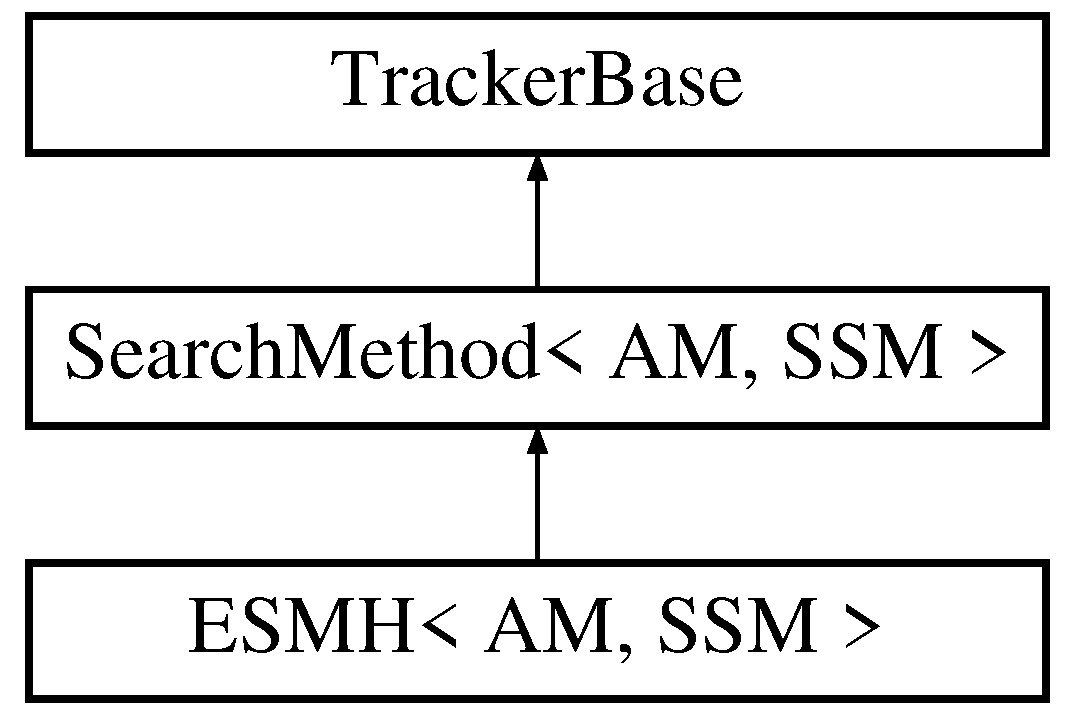
\includegraphics[height=3.000000cm]{classESMH}
\end{center}
\end{figure}
\subsection*{Public Types}
\begin{DoxyCompactItemize}
\item 
\hypertarget{classESMH_a462c285889008b4f0bb90e5cb9999209}{typedef \hyperlink{structESMHParams}{E\-S\-M\-H\-Params} {\bfseries Param\-Type}}\label{classESMH_a462c285889008b4f0bb90e5cb9999209}

\item 
\hypertarget{classESMH_ade5807b653259fc6e359dd66c5ea2832}{typedef Param\-Type\-::\-Jac\-Type {\bfseries Jac\-Type}}\label{classESMH_ade5807b653259fc6e359dd66c5ea2832}

\item 
\hypertarget{classESMH_aa2ecca0f297a5943d2caab8e733f497e}{typedef Param\-Type\-::\-Hess\-Type {\bfseries Hess\-Type}}\label{classESMH_aa2ecca0f297a5943d2caab8e733f497e}

\end{DoxyCompactItemize}
\subsection*{Public Member Functions}
\begin{DoxyCompactItemize}
\item 
\hypertarget{classESMH_a43853036da62afbc048847b9b0525bf6}{{\bfseries E\-S\-M\-H} (const \hyperlink{structESMHParams}{Param\-Type} $\ast$esm\-\_\-params, const \hyperlink{structAMParams}{A\-M\-Params} $\ast$am\-\_\-params, const \hyperlink{structSSMParams}{S\-S\-M\-Params} $\ast$ssm\-\_\-params)}\label{classESMH_a43853036da62afbc048847b9b0525bf6}

\item 
\hypertarget{classESMH_a2655fedddfaa8c11bbebf36fc7d99435}{void {\bfseries initialize} (const cv\-::\-Mat \&corners) override}\label{classESMH_a2655fedddfaa8c11bbebf36fc7d99435}

\item 
\hypertarget{classESMH_ac308eb0f0003c2b3cb515b0d4874db10}{void {\bfseries update} () override}\label{classESMH_ac308eb0f0003c2b3cb515b0d4874db10}

\end{DoxyCompactItemize}
\subsection*{Public Attributes}
\begin{DoxyCompactItemize}
\item 
\hypertarget{classESMH_a219054c57568def4e70a0648c24508ca}{\hyperlink{structESMHParams}{Param\-Type} {\bfseries params}}\label{classESMH_a219054c57568def4e70a0648c24508ca}

\item 
\hypertarget{classESMH_aeb4d26f04f7342c844e465b5be7e5bd2}{int {\bfseries frame\-\_\-id}}\label{classESMH_aeb4d26f04f7342c844e465b5be7e5bd2}

\item 
\hypertarget{classESMH_a12d17ae5a89de7017f728e11b02d703f}{Vector\-Xc {\bfseries pix\-\_\-mask2}}\label{classESMH_a12d17ae5a89de7017f728e11b02d703f}

\item 
\hypertarget{classESMH_aff7a27546fb557d1caee79cf8aeeab71}{Vector\-Xb {\bfseries pix\-\_\-mask}}\label{classESMH_aff7a27546fb557d1caee79cf8aeeab71}

\item 
\hypertarget{classESMH_a70f43fde224bfa1dd32558d6c8c42bb6}{Vector\-Xd {\bfseries rel\-\_\-pix\-\_\-diff}}\label{classESMH_a70f43fde224bfa1dd32558d6c8c42bb6}

\item 
\hypertarget{classESMH_aae20e3d5a7f1ad9b2548cd647092d076}{double {\bfseries max\-\_\-pix\-\_\-diff}}\label{classESMH_aae20e3d5a7f1ad9b2548cd647092d076}

\item 
\hypertarget{classESMH_ae3b0d2f6491dadc762d819b7fe824a31}{Matrix24d {\bfseries prev\-\_\-corners}}\label{classESMH_ae3b0d2f6491dadc762d819b7fe824a31}

\item 
Matrix\-Xd \hyperlink{classESMH_a705f1088f5a2a311463bfb9c59967941}{init\-\_\-pix\-\_\-jacobian}
\begin{DoxyCompactList}\small\item\em N x S jacobians of the pixel values w.\-r.\-t the S\-S\-M state vector where N = resx $\ast$ resy is the no. \end{DoxyCompactList}\item 
\hypertarget{classESMH_a08864655ce72855f5a692368e9f96bb6}{Matrix\-Xd {\bfseries curr\-\_\-pix\-\_\-jacobian}}\label{classESMH_a08864655ce72855f5a692368e9f96bb6}

\item 
\hypertarget{classESMH_a2d91cb739ee987432da7e95dea5b13ae}{Matrix\-Xd {\bfseries mean\-\_\-pix\-\_\-jacobian}}\label{classESMH_a2d91cb739ee987432da7e95dea5b13ae}

\item 
\hypertarget{classESMH_a4bb14113f170c065e182d84c6bfff9fe}{Matrix\-Xd {\bfseries init\-\_\-pix\-\_\-hessian}}\label{classESMH_a4bb14113f170c065e182d84c6bfff9fe}

\item 
\hypertarget{classESMH_a95468d74c34e74a5f229961f8d090502}{Matrix\-Xd {\bfseries curr\-\_\-pix\-\_\-hessian}}\label{classESMH_a95468d74c34e74a5f229961f8d090502}

\item 
\hypertarget{classESMH_a6e1297817fc28659c443e992255fd7d2}{Matrix\-Xd {\bfseries mean\-\_\-pix\-\_\-hessian}}\label{classESMH_a6e1297817fc28659c443e992255fd7d2}

\item 
\hypertarget{classESMH_a0ec68b4ff62ff30a318148dbbf1a605f}{Vector\-Xd {\bfseries ssm\-\_\-update}}\label{classESMH_a0ec68b4ff62ff30a318148dbbf1a605f}

\item 
\hypertarget{classESMH_a4eca65fbf26a66bdaba80c6de599aa82}{Row\-Vector\-Xd \hyperlink{classESMH_a4eca65fbf26a66bdaba80c6de599aa82}{jacobian}}\label{classESMH_a4eca65fbf26a66bdaba80c6de599aa82}

\begin{DoxyCompactList}\small\item\em 1 x S Jacobian of the A\-M error norm w.\-r.\-t. S\-S\-M state vector \end{DoxyCompactList}\item 
\hypertarget{classESMH_a3f378f0d6bc6f9a5704a92f1c822d5d6}{Matrix\-Xd \hyperlink{classESMH_a3f378f0d6bc6f9a5704a92f1c822d5d6}{hessian}}\label{classESMH_a3f378f0d6bc6f9a5704a92f1c822d5d6}

\begin{DoxyCompactList}\small\item\em S x S Hessian of the A\-M error norm w.\-r.\-t. S\-S\-M state vector. \end{DoxyCompactList}\item 
\hypertarget{classESMH_ab5ed5bf94eaca5895a1845aaee24fd7d}{Matrix\-Xd {\bfseries init\-\_\-self\-\_\-hessian}}\label{classESMH_ab5ed5bf94eaca5895a1845aaee24fd7d}

\end{DoxyCompactItemize}
\subsection*{Additional Inherited Members}


\subsection{Member Data Documentation}
\hypertarget{classESMH_a705f1088f5a2a311463bfb9c59967941}{\index{E\-S\-M\-H@{E\-S\-M\-H}!init\-\_\-pix\-\_\-jacobian@{init\-\_\-pix\-\_\-jacobian}}
\index{init\-\_\-pix\-\_\-jacobian@{init\-\_\-pix\-\_\-jacobian}!ESMH@{E\-S\-M\-H}}
\subsubsection[{init\-\_\-pix\-\_\-jacobian}]{\setlength{\rightskip}{0pt plus 5cm}template$<$class A\-M , class S\-S\-M $>$ Matrix\-Xd {\bf E\-S\-M\-H}$<$ A\-M, S\-S\-M $>$\-::init\-\_\-pix\-\_\-jacobian}}\label{classESMH_a705f1088f5a2a311463bfb9c59967941}


N x S jacobians of the pixel values w.\-r.\-t the S\-S\-M state vector where N = resx $\ast$ resy is the no. 

of pixels in the object patch 

The documentation for this class was generated from the following file\-:\begin{DoxyCompactItemize}
\item 
S\-M/include/mtf/\-S\-M/E\-S\-M\-H.\-h\end{DoxyCompactItemize}

\hypertarget{structESMHParams}{\section{E\-S\-M\-H\-Params Struct Reference}
\label{structESMHParams}\index{E\-S\-M\-H\-Params@{E\-S\-M\-H\-Params}}
}
\subsection*{Public Types}
\begin{DoxyCompactItemize}
\item 
enum {\bfseries Jac\-Type} \{ {\bfseries Original}, 
{\bfseries Diff\-Of\-Jacs}
 \}
\item 
enum {\bfseries Hess\-Type} \{ \\*
{\bfseries Original}, 
{\bfseries Sum\-Of\-Std}, 
{\bfseries Sum\-Of\-Self}, 
{\bfseries Initial\-Self}, 
\\*
{\bfseries Current\-Self}, 
{\bfseries Std}
 \}
\end{DoxyCompactItemize}
\subsection*{Public Member Functions}
\begin{DoxyCompactItemize}
\item 
\hyperlink{structESMHParams_a2146f0179851fd0958568f85261a4db2}{E\-S\-M\-H\-Params} (int \-\_\-max\-\_\-iters, double \-\_\-epsilon, Jac\-Type \-\_\-jac\-\_\-type, Hess\-Type \-\_\-hess\-\_\-type, bool \-\_\-sec\-\_\-ord\-\_\-hess, bool \-\_\-enable\-\_\-spi, double \-\_\-spi\-\_\-thresh, bool \-\_\-debug\-\_\-mode)
\begin{DoxyCompactList}\small\item\em decides whether logging data will be printed for debugging purposes; \end{DoxyCompactList}\item 
\hypertarget{structESMHParams_afd14946b9af7647cdb5308ed749271ab}{{\bfseries E\-S\-M\-H\-Params} (\hyperlink{structESMHParams}{E\-S\-M\-H\-Params} $\ast$params=nullptr)}\label{structESMHParams_afd14946b9af7647cdb5308ed749271ab}

\end{DoxyCompactItemize}
\subsection*{Public Attributes}
\begin{DoxyCompactItemize}
\item 
\hypertarget{structESMHParams_a8f45f0d4af3d09955181b5d5b25ecae2}{int {\bfseries max\-\_\-iters}}\label{structESMHParams_a8f45f0d4af3d09955181b5d5b25ecae2}

\item 
\hypertarget{structESMHParams_aa8d2c4ca1b1d2cce26b10ee1a8e09b9d}{double \hyperlink{structESMHParams_aa8d2c4ca1b1d2cce26b10ee1a8e09b9d}{epsilon}}\label{structESMHParams_aa8d2c4ca1b1d2cce26b10ee1a8e09b9d}

\begin{DoxyCompactList}\small\item\em maximum iterations of the \hyperlink{classESMH}{E\-S\-M\-H} algorithm to run for each frame \end{DoxyCompactList}\item 
\hypertarget{structESMHParams_a9538b538978dc781dc77513615655aea}{Jac\-Type \hyperlink{structESMHParams_a9538b538978dc781dc77513615655aea}{jac\-\_\-type}}\label{structESMHParams_a9538b538978dc781dc77513615655aea}

\begin{DoxyCompactList}\small\item\em maximum L1 norm of the state update vector at which to stop the iterations \end{DoxyCompactList}\item 
\hypertarget{structESMHParams_a1dce2f640a33132ac0010c4cbf0820b9}{Hess\-Type {\bfseries hess\-\_\-type}}\label{structESMHParams_a1dce2f640a33132ac0010c4cbf0820b9}

\item 
\hypertarget{structESMHParams_a5c2afd807d9f69d32d6bf7d98c6ddfa5}{bool {\bfseries sec\-\_\-ord\-\_\-hess}}\label{structESMHParams_a5c2afd807d9f69d32d6bf7d98c6ddfa5}

\item 
\hypertarget{structESMHParams_a1486ac30f592f10f63b0f27293c01b70}{bool {\bfseries enable\-\_\-spi}}\label{structESMHParams_a1486ac30f592f10f63b0f27293c01b70}

\item 
\hypertarget{structESMHParams_a270fb82685b55161011b6cc22d106e64}{double {\bfseries spi\-\_\-thresh}}\label{structESMHParams_a270fb82685b55161011b6cc22d106e64}

\item 
\hypertarget{structESMHParams_ad7f8a1b911f8df3f2b5c3ce4c31e9d4e}{bool {\bfseries debug\-\_\-mode}}\label{structESMHParams_ad7f8a1b911f8df3f2b5c3ce4c31e9d4e}

\end{DoxyCompactItemize}


\subsection{Constructor \& Destructor Documentation}
\hypertarget{structESMHParams_a2146f0179851fd0958568f85261a4db2}{\index{E\-S\-M\-H\-Params@{E\-S\-M\-H\-Params}!E\-S\-M\-H\-Params@{E\-S\-M\-H\-Params}}
\index{E\-S\-M\-H\-Params@{E\-S\-M\-H\-Params}!ESMHParams@{E\-S\-M\-H\-Params}}
\subsubsection[{E\-S\-M\-H\-Params}]{\setlength{\rightskip}{0pt plus 5cm}E\-S\-M\-H\-Params\-::\-E\-S\-M\-H\-Params (
\begin{DoxyParamCaption}
\item[{int}]{\-\_\-max\-\_\-iters, }
\item[{double}]{\-\_\-epsilon, }
\item[{Jac\-Type}]{\-\_\-jac\-\_\-type, }
\item[{Hess\-Type}]{\-\_\-hess\-\_\-type, }
\item[{bool}]{\-\_\-sec\-\_\-ord\-\_\-hess, }
\item[{bool}]{\-\_\-enable\-\_\-spi, }
\item[{double}]{\-\_\-spi\-\_\-thresh, }
\item[{bool}]{\-\_\-debug\-\_\-mode}
\end{DoxyParamCaption}
)\hspace{0.3cm}{\ttfamily [inline]}}}\label{structESMHParams_a2146f0179851fd0958568f85261a4db2}


decides whether logging data will be printed for debugging purposes; 

only matters if logging is enabled at compile time 

The documentation for this struct was generated from the following file\-:\begin{DoxyCompactItemize}
\item 
S\-M/include/mtf/\-S\-M/E\-S\-M\-H.\-h\end{DoxyCompactItemize}

\hypertarget{structESMParams}{\section{E\-S\-M\-Params Struct Reference}
\label{structESMParams}\index{E\-S\-M\-Params@{E\-S\-M\-Params}}
}
\subsection*{Public Types}
\begin{DoxyCompactItemize}
\item 
enum {\bfseries Jac\-Type} \{ {\bfseries Original}, 
{\bfseries Diff\-Of\-Jacs}
 \}
\item 
enum {\bfseries Hess\-Type} \{ \\*
{\bfseries Initial\-Self}, 
{\bfseries Current\-Self}, 
{\bfseries Sum\-Of\-Self}, 
{\bfseries Original}, 
\\*
{\bfseries Sum\-Of\-Std}, 
{\bfseries Std}
 \}
\end{DoxyCompactItemize}
\subsection*{Public Member Functions}
\begin{DoxyCompactItemize}
\item 
\hyperlink{structESMParams_a28ec1cebb9e00b95b5155871afeaec6c}{E\-S\-M\-Params} (int \-\_\-max\-\_\-iters, double \-\_\-epsilon, Jac\-Type \-\_\-jac\-\_\-type, Hess\-Type \-\_\-hess\-\_\-type, bool \-\_\-sec\-\_\-ord\-\_\-hess, bool \-\_\-chained\-\_\-warp, bool \-\_\-enable\-\_\-spi, double \-\_\-spi\-\_\-thresh, bool \-\_\-debug\-\_\-mode)
\begin{DoxyCompactList}\small\item\em decides whether logging data will be printed for debugging purposes; \end{DoxyCompactList}\item 
\hypertarget{structESMParams_a11c8741a6ea5898281ac135b58d69579}{{\bfseries E\-S\-M\-Params} (const \hyperlink{structESMParams}{E\-S\-M\-Params} $\ast$params=nullptr)}\label{structESMParams_a11c8741a6ea5898281ac135b58d69579}

\end{DoxyCompactItemize}
\subsection*{Static Public Member Functions}
\begin{DoxyCompactItemize}
\item 
\hypertarget{structESMParams_a6ebf3b0596f90032a2ee9203edcb0b55}{static const char $\ast$ {\bfseries to\-String} (Jac\-Type \-\_\-jac\-\_\-type)}\label{structESMParams_a6ebf3b0596f90032a2ee9203edcb0b55}

\item 
\hypertarget{structESMParams_a3253f737890f9aeffe6e0bf2c38bbabf}{static const char $\ast$ {\bfseries to\-String} (Hess\-Type \-\_\-hess\-\_\-type)}\label{structESMParams_a3253f737890f9aeffe6e0bf2c38bbabf}

\end{DoxyCompactItemize}
\subsection*{Public Attributes}
\begin{DoxyCompactItemize}
\item 
\hypertarget{structESMParams_ae103754c629f35a8d9aa56c5911a8dad}{int {\bfseries max\-\_\-iters}}\label{structESMParams_ae103754c629f35a8d9aa56c5911a8dad}

\item 
\hypertarget{structESMParams_ac62ee111bea1d568bb7dda472b9a359d}{double \hyperlink{structESMParams_ac62ee111bea1d568bb7dda472b9a359d}{epsilon}}\label{structESMParams_ac62ee111bea1d568bb7dda472b9a359d}

\begin{DoxyCompactList}\small\item\em maximum iterations of the \hyperlink{classESM}{E\-S\-M} algorithm to run for each frame \end{DoxyCompactList}\item 
\hypertarget{structESMParams_ac8e31e30cd5c89a5a8a869fcea26c106}{Jac\-Type \hyperlink{structESMParams_ac8e31e30cd5c89a5a8a869fcea26c106}{jac\-\_\-type}}\label{structESMParams_ac8e31e30cd5c89a5a8a869fcea26c106}

\begin{DoxyCompactList}\small\item\em maximum L1 norm of the state update vector at which to stop the iterations \end{DoxyCompactList}\item 
\hypertarget{structESMParams_acfd1104eba9263a6e015c01dad0e9a6d}{Hess\-Type {\bfseries hess\-\_\-type}}\label{structESMParams_acfd1104eba9263a6e015c01dad0e9a6d}

\item 
\hypertarget{structESMParams_a5b15bab42649c16dd14908f6480c3249}{bool {\bfseries sec\-\_\-ord\-\_\-hess}}\label{structESMParams_a5b15bab42649c16dd14908f6480c3249}

\item 
\hypertarget{structESMParams_abfad3a90dfe1c58427af20671b996561}{bool {\bfseries chained\-\_\-warp}}\label{structESMParams_abfad3a90dfe1c58427af20671b996561}

\item 
\hypertarget{structESMParams_a37619667562850108fe2c1900ed631ad}{bool {\bfseries enable\-\_\-spi}}\label{structESMParams_a37619667562850108fe2c1900ed631ad}

\item 
\hypertarget{structESMParams_a1138edd38f5a85ccae1cf602abfac851}{double {\bfseries spi\-\_\-thresh}}\label{structESMParams_a1138edd38f5a85ccae1cf602abfac851}

\item 
\hypertarget{structESMParams_a9d621495901e5bd38e3d0ce4ee419b8f}{bool {\bfseries debug\-\_\-mode}}\label{structESMParams_a9d621495901e5bd38e3d0ce4ee419b8f}

\end{DoxyCompactItemize}


\subsection{Constructor \& Destructor Documentation}
\hypertarget{structESMParams_a28ec1cebb9e00b95b5155871afeaec6c}{\index{E\-S\-M\-Params@{E\-S\-M\-Params}!E\-S\-M\-Params@{E\-S\-M\-Params}}
\index{E\-S\-M\-Params@{E\-S\-M\-Params}!ESMParams@{E\-S\-M\-Params}}
\subsubsection[{E\-S\-M\-Params}]{\setlength{\rightskip}{0pt plus 5cm}E\-S\-M\-Params\-::\-E\-S\-M\-Params (
\begin{DoxyParamCaption}
\item[{int}]{\-\_\-max\-\_\-iters, }
\item[{double}]{\-\_\-epsilon, }
\item[{Jac\-Type}]{\-\_\-jac\-\_\-type, }
\item[{Hess\-Type}]{\-\_\-hess\-\_\-type, }
\item[{bool}]{\-\_\-sec\-\_\-ord\-\_\-hess, }
\item[{bool}]{\-\_\-chained\-\_\-warp, }
\item[{bool}]{\-\_\-enable\-\_\-spi, }
\item[{double}]{\-\_\-spi\-\_\-thresh, }
\item[{bool}]{\-\_\-debug\-\_\-mode}
\end{DoxyParamCaption}
)}}\label{structESMParams_a28ec1cebb9e00b95b5155871afeaec6c}


decides whether logging data will be printed for debugging purposes; 

only matters if logging is enabled at compile time 

The documentation for this struct was generated from the following file\-:\begin{DoxyCompactItemize}
\item 
S\-M/include/mtf/\-S\-M/E\-S\-M\-Params.\-h\end{DoxyCompactItemize}

\hypertarget{classFALK}{\section{F\-A\-L\-K$<$ A\-M, S\-S\-M $>$ Class Template Reference}
\label{classFALK}\index{F\-A\-L\-K$<$ A\-M, S\-S\-M $>$@{F\-A\-L\-K$<$ A\-M, S\-S\-M $>$}}
}
Inheritance diagram for F\-A\-L\-K$<$ A\-M, S\-S\-M $>$\-:\begin{figure}[H]
\begin{center}
\leavevmode
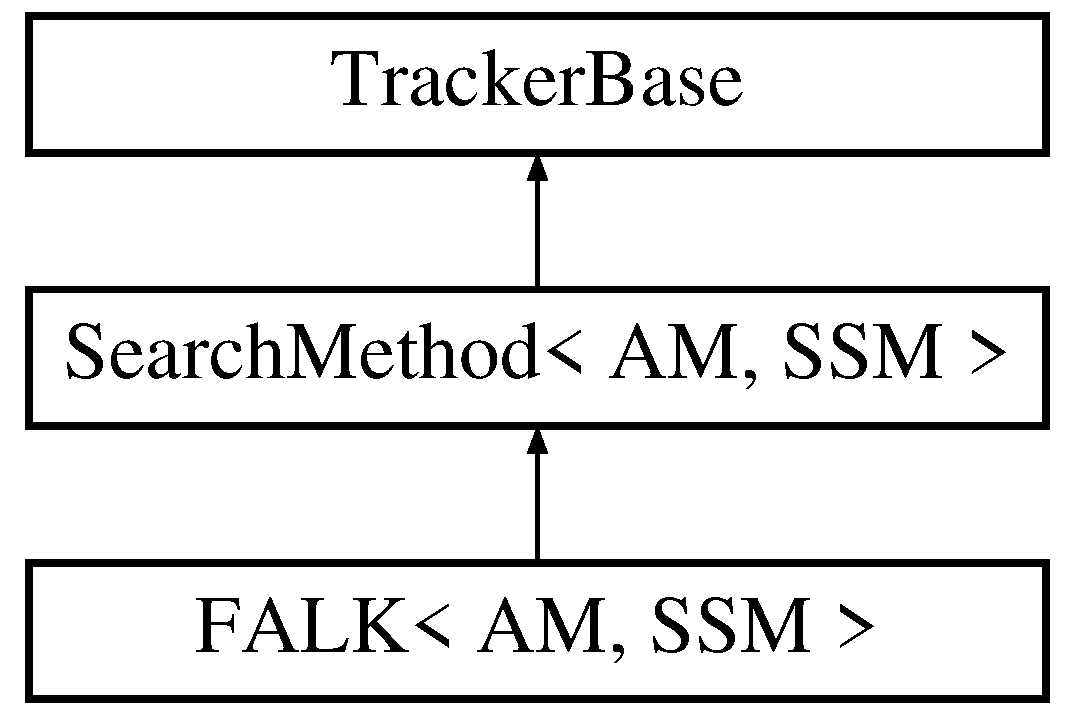
\includegraphics[height=3.000000cm]{classFALK}
\end{center}
\end{figure}
\subsection*{Public Types}
\begin{DoxyCompactItemize}
\item 
\hypertarget{classFALK_aa5546fa0c3e416e395f4c7b6bdac83b0}{typedef \hyperlink{structFALKParams}{F\-A\-L\-K\-Params} {\bfseries Param\-Type}}\label{classFALK_aa5546fa0c3e416e395f4c7b6bdac83b0}

\item 
\hypertarget{classFALK_aabe59f8aed651a0bb95bea0827371369}{typedef Param\-Type\-::\-Hess\-Type {\bfseries Hess\-Type}}\label{classFALK_aabe59f8aed651a0bb95bea0827371369}

\end{DoxyCompactItemize}
\subsection*{Public Member Functions}
\begin{DoxyCompactItemize}
\item 
\hypertarget{classFALK_a934cc0db0b9c6c403688049ee1c16610}{{\bfseries F\-A\-L\-K} (const \hyperlink{structFALKParams}{Param\-Type} $\ast$falk\-\_\-params=nullptr, const \hyperlink{structAMParams}{A\-M\-Params} $\ast$am\-\_\-params=nullptr, const \hyperlink{structSSMParams}{S\-S\-M\-Params} $\ast$ssm\-\_\-params=nullptr)}\label{classFALK_a934cc0db0b9c6c403688049ee1c16610}

\item 
\hypertarget{classFALK_aeb316fca47c41b04699c76c506176831}{void {\bfseries initialize} (const cv\-::\-Mat \&corners) override}\label{classFALK_aeb316fca47c41b04699c76c506176831}

\item 
\hypertarget{classFALK_a382f20a48618e7d9b3fd3f4fdbdacb7c}{void {\bfseries update} () override}\label{classFALK_a382f20a48618e7d9b3fd3f4fdbdacb7c}

\end{DoxyCompactItemize}
\subsection*{Public Attributes}
\begin{DoxyCompactItemize}
\item 
\hypertarget{classFALK_a15721db6c945f66c847b76e7a55e850e}{\hyperlink{structFALKParams}{Param\-Type} {\bfseries params}}\label{classFALK_a15721db6c945f66c847b76e7a55e850e}

\end{DoxyCompactItemize}
\subsection*{Protected Attributes}
\begin{DoxyCompactItemize}
\item 
\hypertarget{classFALK_a6fd04c140915ae2c95e2ffe4954ea14b}{Row\-Vector\-Xd \hyperlink{classFALK_a6fd04c140915ae2c95e2ffe4954ea14b}{jacobian}}\label{classFALK_a6fd04c140915ae2c95e2ffe4954ea14b}

\begin{DoxyCompactList}\small\item\em 1 x S Jacobian of the A\-M similarity function w.\-r.\-t. S\-S\-M state vector \end{DoxyCompactList}\item 
\hypertarget{classFALK_a9e7d06e0380210c65dd78c3661607c98}{Matrix\-Xd \hyperlink{classFALK_a9e7d06e0380210c65dd78c3661607c98}{hessian}}\label{classFALK_a9e7d06e0380210c65dd78c3661607c98}

\begin{DoxyCompactList}\small\item\em S x S Hessian of the A\-M similarity function w.\-r.\-t. S\-S\-M state vector. \end{DoxyCompactList}\item 
\hypertarget{classFALK_a60ac78fa548216594bac3186d8952517}{Matrix\-Xd \hyperlink{classFALK_a60ac78fa548216594bac3186d8952517}{init\-\_\-pix\-\_\-jacobian}}\label{classFALK_a60ac78fa548216594bac3186d8952517}

\begin{DoxyCompactList}\small\item\em N x S jacobians of the pixel values w.\-r.\-t the S\-S\-M state vector. \end{DoxyCompactList}\item 
\hypertarget{classFALK_a1818731dc14e4cc2251b5ab6a8fc13c8}{Matrix\-Xd {\bfseries curr\-\_\-pix\-\_\-jacobian}}\label{classFALK_a1818731dc14e4cc2251b5ab6a8fc13c8}

\item 
\hypertarget{classFALK_a684f543f251d55ed03b3d485066c53c6}{Matrix\-Xd \hyperlink{classFALK_a684f543f251d55ed03b3d485066c53c6}{init\-\_\-pix\-\_\-hessian}}\label{classFALK_a684f543f251d55ed03b3d485066c53c6}

\begin{DoxyCompactList}\small\item\em N x S x S hessians of the pixel values w.\-r.\-t the S\-S\-M state vector stored as a (S$\ast$\-S) x N 2\-D matrix. \end{DoxyCompactList}\item 
\hypertarget{classFALK_a47e18fd05f0ee46ad2b561db3a103bd3}{Matrix\-Xd {\bfseries curr\-\_\-pix\-\_\-hessian}}\label{classFALK_a47e18fd05f0ee46ad2b561db3a103bd3}

\item 
\hypertarget{classFALK_a70884ec27965ec6867cc254600063943}{Matrix24d {\bfseries prev\-\_\-corners}}\label{classFALK_a70884ec27965ec6867cc254600063943}

\item 
\hypertarget{classFALK_ac436569dcc13c6b903893934938c3c36}{Vector\-Xd {\bfseries ssm\-\_\-update}}\label{classFALK_ac436569dcc13c6b903893934938c3c36}

\item 
\hypertarget{classFALK_a6b36dc5832e82e11ee417362fcc3aa7f}{Matrix3d {\bfseries warp\-\_\-update}}\label{classFALK_a6b36dc5832e82e11ee417362fcc3aa7f}

\item 
\hypertarget{classFALK_a3035161f4a1c1d4c7dc12a42b5388303}{int {\bfseries frame\-\_\-id}}\label{classFALK_a3035161f4a1c1d4c7dc12a42b5388303}

\end{DoxyCompactItemize}


The documentation for this class was generated from the following file\-:\begin{DoxyCompactItemize}
\item 
S\-M/include/mtf/\-S\-M/F\-A\-L\-K.\-h\end{DoxyCompactItemize}

\hypertarget{structFALKParams}{\section{F\-A\-L\-K\-Params Struct Reference}
\label{structFALKParams}\index{F\-A\-L\-K\-Params@{F\-A\-L\-K\-Params}}
}
\subsection*{Public Types}
\begin{DoxyCompactItemize}
\item 
enum {\bfseries Hess\-Type} \{ {\bfseries Initial\-Self}, 
{\bfseries Current\-Self}, 
{\bfseries Std}
 \}
\end{DoxyCompactItemize}
\subsection*{Public Member Functions}
\begin{DoxyCompactItemize}
\item 
\hyperlink{structFALKParams_a5478ddf0e62e74d539aa39fca02f79b0}{F\-A\-L\-K\-Params} (int \-\_\-max\-\_\-iters, double \-\_\-epsilon, Hess\-Type \-\_\-hess\-\_\-type, bool \-\_\-sec\-\_\-ord\-\_\-hess, bool \-\_\-show\-\_\-grid, bool \-\_\-show\-\_\-patch, double \-\_\-patch\-\_\-resize\-\_\-factor, bool \-\_\-write\-\_\-frames, bool \-\_\-upd\-\_\-templ, bool \-\_\-debug\-\_\-mode)
\begin{DoxyCompactList}\small\item\em decides whether logging data will be printed for debugging purposes; \end{DoxyCompactList}\item 
\hypertarget{structFALKParams_a45cf22a7c4e26dc85306879d348429cd}{{\bfseries F\-A\-L\-K\-Params} (const \hyperlink{structFALKParams}{F\-A\-L\-K\-Params} $\ast$params=nullptr)}\label{structFALKParams_a45cf22a7c4e26dc85306879d348429cd}

\end{DoxyCompactItemize}
\subsection*{Public Attributes}
\begin{DoxyCompactItemize}
\item 
\hypertarget{structFALKParams_afb17dcf190ea13e6ceabd1e4feddfc4a}{int {\bfseries max\-\_\-iters}}\label{structFALKParams_afb17dcf190ea13e6ceabd1e4feddfc4a}

\item 
\hypertarget{structFALKParams_a83fc27e9249e2cad6a717d298b35dfaf}{double \hyperlink{structFALKParams_a83fc27e9249e2cad6a717d298b35dfaf}{epsilon}}\label{structFALKParams_a83fc27e9249e2cad6a717d298b35dfaf}

\begin{DoxyCompactList}\small\item\em maximum iterations of the \hyperlink{classFALK}{F\-A\-L\-K} algorithm to run for each frame \end{DoxyCompactList}\item 
\hypertarget{structFALKParams_aa3fe6c35c22f76ecde01d92f94380c32}{Hess\-Type \hyperlink{structFALKParams_aa3fe6c35c22f76ecde01d92f94380c32}{hess\-\_\-type}}\label{structFALKParams_aa3fe6c35c22f76ecde01d92f94380c32}

\begin{DoxyCompactList}\small\item\em maximum L1 norm of the state update vector at which to stop the iterations \end{DoxyCompactList}\item 
\hypertarget{structFALKParams_a06525c0f52efb447003b9781af356912}{bool {\bfseries sec\-\_\-ord\-\_\-hess}}\label{structFALKParams_a06525c0f52efb447003b9781af356912}

\item 
\hypertarget{structFALKParams_a27e82e7de3bb6734a4577769aebb2e03}{bool {\bfseries show\-\_\-grid}}\label{structFALKParams_a27e82e7de3bb6734a4577769aebb2e03}

\item 
\hypertarget{structFALKParams_a22855504c3ca706015338c7fb7bbd22a}{bool {\bfseries show\-\_\-patch}}\label{structFALKParams_a22855504c3ca706015338c7fb7bbd22a}

\item 
\hypertarget{structFALKParams_a8c43fe1b56fef51b74cb547092b49537}{double {\bfseries patch\-\_\-resize\-\_\-factor}}\label{structFALKParams_a8c43fe1b56fef51b74cb547092b49537}

\item 
\hypertarget{structFALKParams_a5595139787c7099817523e1539c1e15d}{bool {\bfseries write\-\_\-frames}}\label{structFALKParams_a5595139787c7099817523e1539c1e15d}

\item 
\hypertarget{structFALKParams_a3237674dfaecae009b4bedc1bdbe3dbd}{bool {\bfseries upd\-\_\-templ}}\label{structFALKParams_a3237674dfaecae009b4bedc1bdbe3dbd}

\item 
\hypertarget{structFALKParams_aa81d5bdda8acbae63aa9e79bfff50a63}{bool {\bfseries debug\-\_\-mode}}\label{structFALKParams_aa81d5bdda8acbae63aa9e79bfff50a63}

\end{DoxyCompactItemize}


\subsection{Constructor \& Destructor Documentation}
\hypertarget{structFALKParams_a5478ddf0e62e74d539aa39fca02f79b0}{\index{F\-A\-L\-K\-Params@{F\-A\-L\-K\-Params}!F\-A\-L\-K\-Params@{F\-A\-L\-K\-Params}}
\index{F\-A\-L\-K\-Params@{F\-A\-L\-K\-Params}!FALKParams@{F\-A\-L\-K\-Params}}
\subsubsection[{F\-A\-L\-K\-Params}]{\setlength{\rightskip}{0pt plus 5cm}F\-A\-L\-K\-Params\-::\-F\-A\-L\-K\-Params (
\begin{DoxyParamCaption}
\item[{int}]{\-\_\-max\-\_\-iters, }
\item[{double}]{\-\_\-epsilon, }
\item[{Hess\-Type}]{\-\_\-hess\-\_\-type, }
\item[{bool}]{\-\_\-sec\-\_\-ord\-\_\-hess, }
\item[{bool}]{\-\_\-show\-\_\-grid, }
\item[{bool}]{\-\_\-show\-\_\-patch, }
\item[{double}]{\-\_\-patch\-\_\-resize\-\_\-factor, }
\item[{bool}]{\-\_\-write\-\_\-frames, }
\item[{bool}]{\-\_\-upd\-\_\-templ, }
\item[{bool}]{\-\_\-debug\-\_\-mode}
\end{DoxyParamCaption}
)}}\label{structFALKParams_a5478ddf0e62e74d539aa39fca02f79b0}


decides whether logging data will be printed for debugging purposes; 

only matters if logging is enabled at compile time 

The documentation for this struct was generated from the following file\-:\begin{DoxyCompactItemize}
\item 
S\-M/include/mtf/\-S\-M/F\-A\-L\-K\-Params.\-h\end{DoxyCompactItemize}

\hypertarget{classFCLK}{\section{F\-C\-L\-K$<$ A\-M, S\-S\-M $>$ Class Template Reference}
\label{classFCLK}\index{F\-C\-L\-K$<$ A\-M, S\-S\-M $>$@{F\-C\-L\-K$<$ A\-M, S\-S\-M $>$}}
}
Inheritance diagram for F\-C\-L\-K$<$ A\-M, S\-S\-M $>$\-:\begin{figure}[H]
\begin{center}
\leavevmode
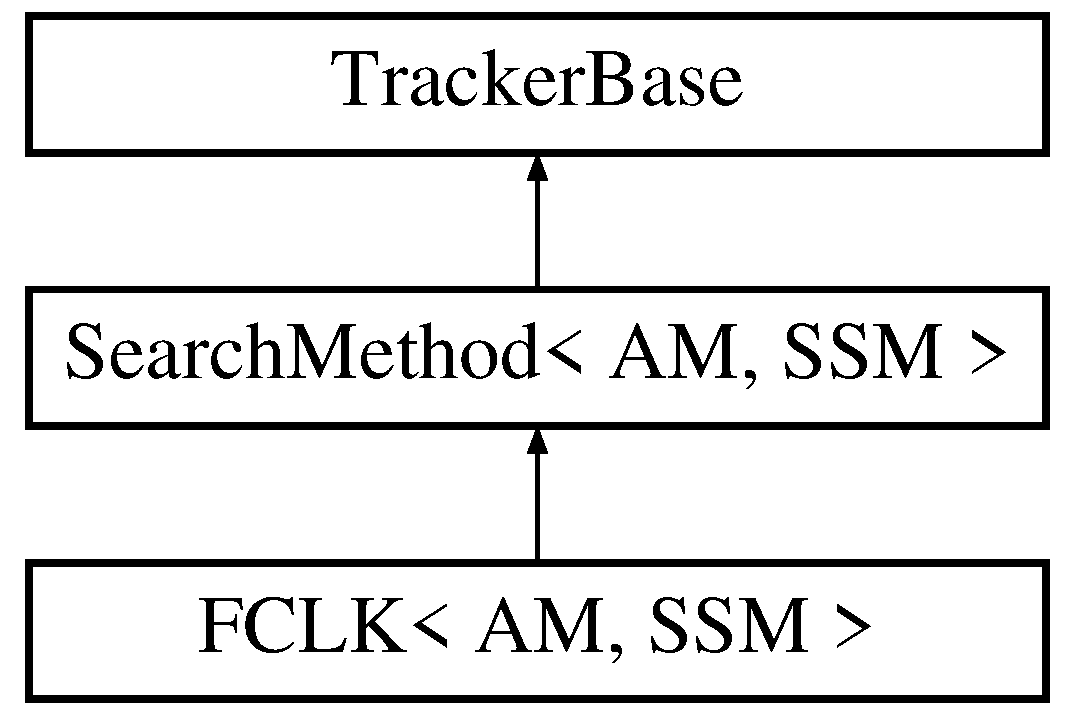
\includegraphics[height=3.000000cm]{classFCLK}
\end{center}
\end{figure}
\subsection*{Public Types}
\begin{DoxyCompactItemize}
\item 
\hypertarget{classFCLK_a1287e06bf398f08c3b14dc00d0097e29}{typedef \hyperlink{structFCLKParams}{F\-C\-L\-K\-Params} {\bfseries Param\-Type}}\label{classFCLK_a1287e06bf398f08c3b14dc00d0097e29}

\item 
\hypertarget{classFCLK_a4934faeb78685cf910d63485c2c0430a}{typedef Param\-Type\-::\-Hess\-Type {\bfseries Hess\-Type}}\label{classFCLK_a4934faeb78685cf910d63485c2c0430a}

\end{DoxyCompactItemize}
\subsection*{Public Member Functions}
\begin{DoxyCompactItemize}
\item 
\hypertarget{classFCLK_ab576a57be4effa4634db54c8520d95f8}{{\bfseries F\-C\-L\-K} (const \hyperlink{structFCLKParams}{Param\-Type} $\ast$fclk\-\_\-params=nullptr, const \hyperlink{structAMParams}{A\-M\-Params} $\ast$am\-\_\-params=nullptr, const \hyperlink{structSSMParams}{S\-S\-M\-Params} $\ast$ssm\-\_\-params=nullptr)}\label{classFCLK_ab576a57be4effa4634db54c8520d95f8}

\item 
\hypertarget{classFCLK_a9bd3f486a633286c19a13c68b9d119c2}{void {\bfseries initialize} (const cv\-::\-Mat \&corners) override}\label{classFCLK_a9bd3f486a633286c19a13c68b9d119c2}

\item 
\hypertarget{classFCLK_ab22a424466a2e49de4e2817d776222c8}{void {\bfseries update} () override}\label{classFCLK_ab22a424466a2e49de4e2817d776222c8}

\item 
\hypertarget{classFCLK_aa4605cd9189de98673a1966b34e1791d}{void {\bfseries set\-Region} (const cv\-::\-Mat \&corners) override}\label{classFCLK_aa4605cd9189de98673a1966b34e1791d}

\end{DoxyCompactItemize}
\subsection*{Public Attributes}
\begin{DoxyCompactItemize}
\item 
\hypertarget{classFCLK_adad325d145a4cf9f0c41c0667be1a336}{\hyperlink{structFCLKParams}{Param\-Type} {\bfseries params}}\label{classFCLK_adad325d145a4cf9f0c41c0667be1a336}

\item 
\hypertarget{classFCLK_a777a27f6007e54b927e24a97ef9ed9ac}{Row\-Vector\-Xd \hyperlink{classFCLK_a777a27f6007e54b927e24a97ef9ed9ac}{jacobian}}\label{classFCLK_a777a27f6007e54b927e24a97ef9ed9ac}

\begin{DoxyCompactList}\small\item\em 1 x S Jacobian of the appearance model w.\-r.\-t. S\-S\-M state vector \end{DoxyCompactList}\item 
\hypertarget{classFCLK_ac629b1e7f1a5f06630520ee0211c50d3}{Matrix\-Xd \hyperlink{classFCLK_ac629b1e7f1a5f06630520ee0211c50d3}{hessian}}\label{classFCLK_ac629b1e7f1a5f06630520ee0211c50d3}

\begin{DoxyCompactList}\small\item\em S x S Hessian of the appearance model w.\-r.\-t. S\-S\-M state vector. \end{DoxyCompactList}\item 
\hypertarget{classFCLK_a3ef0d3c279c07129b0608d88ab33b186}{Matrix\-Xd \hyperlink{classFCLK_a3ef0d3c279c07129b0608d88ab33b186}{init\-\_\-pix\-\_\-jacobian}}\label{classFCLK_a3ef0d3c279c07129b0608d88ab33b186}

\begin{DoxyCompactList}\small\item\em N x S jacobians of the pix values w.\-r.\-t the S\-S\-M state vector. \end{DoxyCompactList}\item 
\hypertarget{classFCLK_a5057c409c97bd8b00860c7a1b07e7d1c}{Matrix\-Xd {\bfseries curr\-\_\-pix\-\_\-jacobian}}\label{classFCLK_a5057c409c97bd8b00860c7a1b07e7d1c}

\item 
\hypertarget{classFCLK_acda983da6ae75475480a14b76698b9d5}{Matrix\-Xd {\bfseries curr\-\_\-pix\-\_\-jacobian\-\_\-new}}\label{classFCLK_acda983da6ae75475480a14b76698b9d5}

\item 
\hypertarget{classFCLK_ac4141b5f334dbffb97e46dac6aa493f5}{Matrix\-Xd \hyperlink{classFCLK_ac4141b5f334dbffb97e46dac6aa493f5}{init\-\_\-pix\-\_\-hessian}}\label{classFCLK_ac4141b5f334dbffb97e46dac6aa493f5}

\begin{DoxyCompactList}\small\item\em N x S x S hessians of the pixel values w.\-r.\-t the S\-S\-M state vector stored as a (S$\ast$\-S) x N 2\-D matrix. \end{DoxyCompactList}\item 
\hypertarget{classFCLK_a838cd36940df8b2b5063854bf602ce59}{Matrix\-Xd {\bfseries curr\-\_\-pix\-\_\-hessian}}\label{classFCLK_a838cd36940df8b2b5063854bf602ce59}

\item 
\hypertarget{classFCLK_aaf7115aebc182fb22c106e605c229a26}{Matrix24d {\bfseries prev\-\_\-corners}}\label{classFCLK_aaf7115aebc182fb22c106e605c229a26}

\item 
\hypertarget{classFCLK_a1b1f9ca4b00aea40e9ae738bf1fa712c}{Vector\-Xd {\bfseries ssm\-\_\-update}}\label{classFCLK_a1b1f9ca4b00aea40e9ae738bf1fa712c}

\item 
\hypertarget{classFCLK_afa536f739236a83f70c266ab809e1dad}{int {\bfseries frame\-\_\-id}}\label{classFCLK_afa536f739236a83f70c266ab809e1dad}

\end{DoxyCompactItemize}
\subsection*{Additional Inherited Members}


The documentation for this class was generated from the following file\-:\begin{DoxyCompactItemize}
\item 
S\-M/include/mtf/\-S\-M/F\-C\-L\-K.\-h\end{DoxyCompactItemize}

\hypertarget{structFCLKParams}{\section{F\-C\-L\-K\-Params Struct Reference}
\label{structFCLKParams}\index{F\-C\-L\-K\-Params@{F\-C\-L\-K\-Params}}
}
\subsection*{Public Types}
\begin{DoxyCompactItemize}
\item 
enum {\bfseries Hess\-Type} \{ {\bfseries Initial\-Self}, 
{\bfseries Current\-Self}, 
{\bfseries Std}
 \}
\end{DoxyCompactItemize}
\subsection*{Public Member Functions}
\begin{DoxyCompactItemize}
\item 
\hyperlink{structFCLKParams_acbb5c8042e37cabdee9c38ed1e942f66}{F\-C\-L\-K\-Params} (int \-\_\-max\-\_\-iters, double \-\_\-epsilon, Hess\-Type \-\_\-hess\-\_\-type, bool \-\_\-sec\-\_\-ord\-\_\-hess, bool \-\_\-upd\-\_\-templ, bool \-\_\-chained\-\_\-warp, bool \-\_\-leven\-\_\-marq, double \-\_\-lm\-\_\-delta\-\_\-init, double \-\_\-lm\-\_\-delta\-\_\-update, bool \-\_\-write\-\_\-ssm\-\_\-updates, bool \-\_\-show\-\_\-grid, bool \-\_\-show\-\_\-patch, double \-\_\-patch\-\_\-resize\-\_\-factor, bool \-\_\-debug\-\_\-mode)
\begin{DoxyCompactList}\small\item\em decides whether logging data will be printed for debugging purposes; \end{DoxyCompactList}\item 
\hypertarget{structFCLKParams_a95be51bc8643a43893db2dd5dc0462ab}{{\bfseries F\-C\-L\-K\-Params} (const \hyperlink{structFCLKParams}{F\-C\-L\-K\-Params} $\ast$params=nullptr)}\label{structFCLKParams_a95be51bc8643a43893db2dd5dc0462ab}

\end{DoxyCompactItemize}
\subsection*{Static Public Member Functions}
\begin{DoxyCompactItemize}
\item 
\hypertarget{structFCLKParams_afbdb1a18be20ecb53ea2a5284524c4ba}{static const char $\ast$ {\bfseries to\-String} (Hess\-Type \hyperlink{structFCLKParams_a7ff564478a6a523aaa108524b9700443}{hess\-\_\-type})}\label{structFCLKParams_afbdb1a18be20ecb53ea2a5284524c4ba}

\end{DoxyCompactItemize}
\subsection*{Public Attributes}
\begin{DoxyCompactItemize}
\item 
\hypertarget{structFCLKParams_ae28b919859bdf27ea18b4667e2f2bd5b}{int {\bfseries max\-\_\-iters}}\label{structFCLKParams_ae28b919859bdf27ea18b4667e2f2bd5b}

\item 
\hypertarget{structFCLKParams_aade1acbbbc70e4bd3d16f98fdbea48bc}{double \hyperlink{structFCLKParams_aade1acbbbc70e4bd3d16f98fdbea48bc}{epsilon}}\label{structFCLKParams_aade1acbbbc70e4bd3d16f98fdbea48bc}

\begin{DoxyCompactList}\small\item\em maximum iterations of the \hyperlink{classFCLK}{F\-C\-L\-K} algorithm to run for each frame \end{DoxyCompactList}\item 
\hypertarget{structFCLKParams_a7ff564478a6a523aaa108524b9700443}{Hess\-Type \hyperlink{structFCLKParams_a7ff564478a6a523aaa108524b9700443}{hess\-\_\-type}}\label{structFCLKParams_a7ff564478a6a523aaa108524b9700443}

\begin{DoxyCompactList}\small\item\em maximum L1 norm of the state update vector at which to stop the iterations \end{DoxyCompactList}\item 
\hypertarget{structFCLKParams_a3bb148d66d5beeb50e505f7672b0b6b8}{bool {\bfseries sec\-\_\-ord\-\_\-hess}}\label{structFCLKParams_a3bb148d66d5beeb50e505f7672b0b6b8}

\item 
\hypertarget{structFCLKParams_a9641117ad4a414a37975865c4ab7a788}{bool {\bfseries chained\-\_\-warp}}\label{structFCLKParams_a9641117ad4a414a37975865c4ab7a788}

\item 
\hypertarget{structFCLKParams_afa9a0d33d4933e32ebb0bbcb4a5bfbf3}{bool {\bfseries leven\-\_\-marq}}\label{structFCLKParams_afa9a0d33d4933e32ebb0bbcb4a5bfbf3}

\item 
\hypertarget{structFCLKParams_a371dc5f3519f88054d804cd76ef19e4a}{double {\bfseries lm\-\_\-delta\-\_\-init}}\label{structFCLKParams_a371dc5f3519f88054d804cd76ef19e4a}

\item 
\hypertarget{structFCLKParams_a2333e9579494fad1692102b89ac50535}{double {\bfseries lm\-\_\-delta\-\_\-update}}\label{structFCLKParams_a2333e9579494fad1692102b89ac50535}

\item 
\hypertarget{structFCLKParams_af5aa8f2d54f5d456382b501ac7b6920b}{bool {\bfseries upd\-\_\-templ}}\label{structFCLKParams_af5aa8f2d54f5d456382b501ac7b6920b}

\item 
\hypertarget{structFCLKParams_a60c72639a531c88a5a9b42c1478b6e90}{bool {\bfseries write\-\_\-ssm\-\_\-updates}}\label{structFCLKParams_a60c72639a531c88a5a9b42c1478b6e90}

\item 
\hypertarget{structFCLKParams_ad30fb54549b55247c6e1a909c4ffca1e}{bool {\bfseries show\-\_\-grid}}\label{structFCLKParams_ad30fb54549b55247c6e1a909c4ffca1e}

\item 
\hypertarget{structFCLKParams_a44327fb3daac9c7eef47ef2898ccaa75}{bool {\bfseries show\-\_\-patch}}\label{structFCLKParams_a44327fb3daac9c7eef47ef2898ccaa75}

\item 
\hypertarget{structFCLKParams_a31a0bebe10e53cd0fdd6144af1e52acf}{double {\bfseries patch\-\_\-resize\-\_\-factor}}\label{structFCLKParams_a31a0bebe10e53cd0fdd6144af1e52acf}

\item 
\hypertarget{structFCLKParams_ace3d9033969fd7bbcba509573e4fdccc}{bool {\bfseries debug\-\_\-mode}}\label{structFCLKParams_ace3d9033969fd7bbcba509573e4fdccc}

\end{DoxyCompactItemize}


\subsection{Constructor \& Destructor Documentation}
\hypertarget{structFCLKParams_acbb5c8042e37cabdee9c38ed1e942f66}{\index{F\-C\-L\-K\-Params@{F\-C\-L\-K\-Params}!F\-C\-L\-K\-Params@{F\-C\-L\-K\-Params}}
\index{F\-C\-L\-K\-Params@{F\-C\-L\-K\-Params}!FCLKParams@{F\-C\-L\-K\-Params}}
\subsubsection[{F\-C\-L\-K\-Params}]{\setlength{\rightskip}{0pt plus 5cm}F\-C\-L\-K\-Params\-::\-F\-C\-L\-K\-Params (
\begin{DoxyParamCaption}
\item[{int}]{\-\_\-max\-\_\-iters, }
\item[{double}]{\-\_\-epsilon, }
\item[{Hess\-Type}]{\-\_\-hess\-\_\-type, }
\item[{bool}]{\-\_\-sec\-\_\-ord\-\_\-hess, }
\item[{bool}]{\-\_\-upd\-\_\-templ, }
\item[{bool}]{\-\_\-chained\-\_\-warp, }
\item[{bool}]{\-\_\-leven\-\_\-marq, }
\item[{double}]{\-\_\-lm\-\_\-delta\-\_\-init, }
\item[{double}]{\-\_\-lm\-\_\-delta\-\_\-update, }
\item[{bool}]{\-\_\-write\-\_\-ssm\-\_\-updates, }
\item[{bool}]{\-\_\-show\-\_\-grid, }
\item[{bool}]{\-\_\-show\-\_\-patch, }
\item[{double}]{\-\_\-patch\-\_\-resize\-\_\-factor, }
\item[{bool}]{\-\_\-debug\-\_\-mode}
\end{DoxyParamCaption}
)}}\label{structFCLKParams_acbb5c8042e37cabdee9c38ed1e942f66}


decides whether logging data will be printed for debugging purposes; 

only matters if logging is enabled at compile time 

The documentation for this struct was generated from the following file\-:\begin{DoxyCompactItemize}
\item 
S\-M/include/mtf/\-S\-M/F\-C\-L\-K\-Params.\-h\end{DoxyCompactItemize}

\hypertarget{classFESM}{\section{F\-E\-S\-M$<$ A\-M, S\-S\-M, H\-T, J\-T $>$ Class Template Reference}
\label{classFESM}\index{F\-E\-S\-M$<$ A\-M, S\-S\-M, H\-T, J\-T $>$@{F\-E\-S\-M$<$ A\-M, S\-S\-M, H\-T, J\-T $>$}}
}
Inheritance diagram for F\-E\-S\-M$<$ A\-M, S\-S\-M, H\-T, J\-T $>$\-:\begin{figure}[H]
\begin{center}
\leavevmode
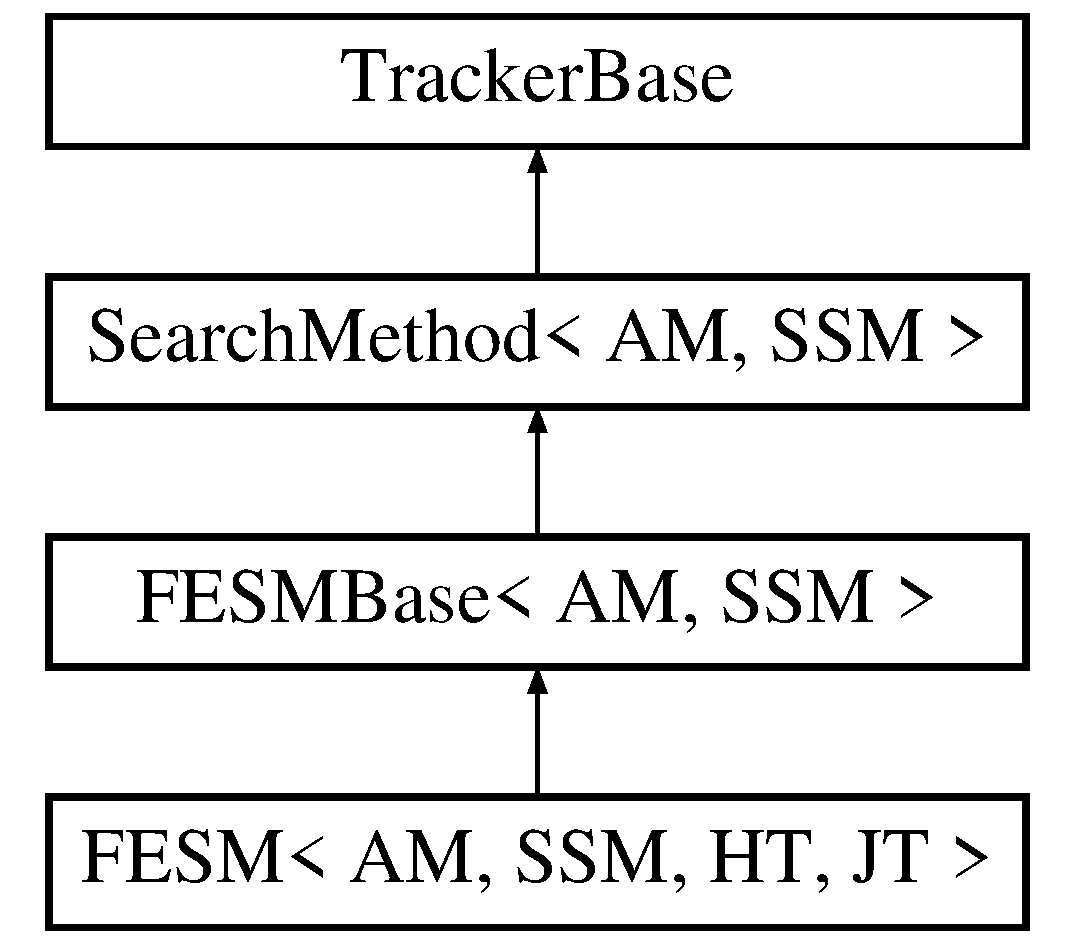
\includegraphics[height=4.000000cm]{classFESM}
\end{center}
\end{figure}
\subsection*{Additional Inherited Members}


The documentation for this class was generated from the following file\-:\begin{DoxyCompactItemize}
\item 
S\-M/include/mtf/\-S\-M/F\-E\-S\-M.\-h\end{DoxyCompactItemize}

\hypertarget{classFESM_3_01AM_00_01SSM_00_01HessT_1_1CurrentSelf_00_01JacT_1_1DiffOfJacs_01_4}{\section{F\-E\-S\-M$<$ A\-M, S\-S\-M, Hess\-T\-:\-:Current\-Self, Jac\-T\-:\-:Diff\-Of\-Jacs $>$ Class Template Reference}
\label{classFESM_3_01AM_00_01SSM_00_01HessT_1_1CurrentSelf_00_01JacT_1_1DiffOfJacs_01_4}\index{F\-E\-S\-M$<$ A\-M, S\-S\-M, Hess\-T\-::\-Current\-Self, Jac\-T\-::\-Diff\-Of\-Jacs $>$@{F\-E\-S\-M$<$ A\-M, S\-S\-M, Hess\-T\-::\-Current\-Self, Jac\-T\-::\-Diff\-Of\-Jacs $>$}}
}
Inheritance diagram for F\-E\-S\-M$<$ A\-M, S\-S\-M, Hess\-T\-:\-:Current\-Self, Jac\-T\-:\-:Diff\-Of\-Jacs $>$\-:\begin{figure}[H]
\begin{center}
\leavevmode
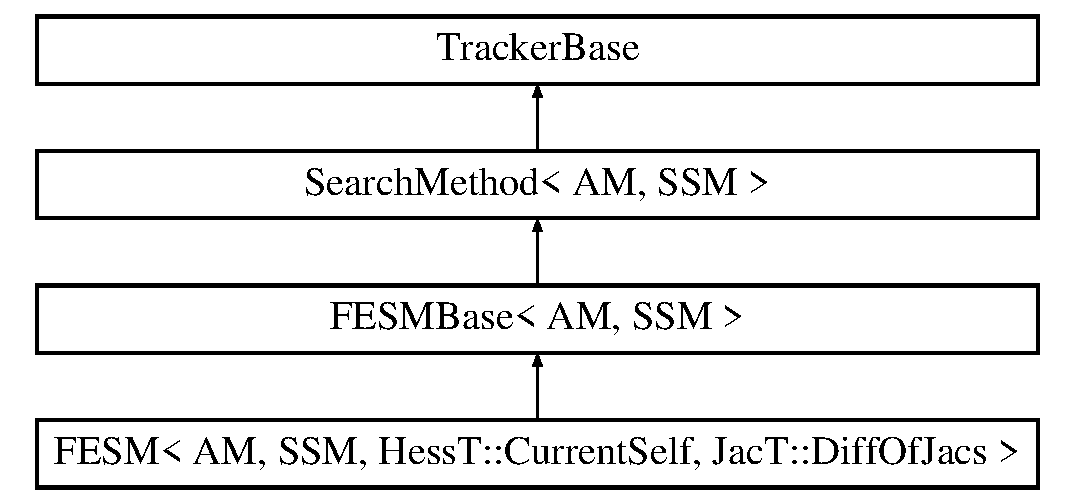
\includegraphics[height=4.000000cm]{classFESM_3_01AM_00_01SSM_00_01HessT_1_1CurrentSelf_00_01JacT_1_1DiffOfJacs_01_4}
\end{center}
\end{figure}
\subsection*{Additional Inherited Members}


The documentation for this class was generated from the following file\-:\begin{DoxyCompactItemize}
\item 
S\-M/include/mtf/\-S\-M/F\-E\-S\-M.\-h\end{DoxyCompactItemize}

\hypertarget{classFESM_3_01AM_00_01SSM_00_01HessT_1_1CurrentSelf_00_01JacT_1_1Original_01_4}{\section{F\-E\-S\-M$<$ A\-M, S\-S\-M, Hess\-T\-:\-:Current\-Self, Jac\-T\-:\-:Original $>$ Class Template Reference}
\label{classFESM_3_01AM_00_01SSM_00_01HessT_1_1CurrentSelf_00_01JacT_1_1Original_01_4}\index{F\-E\-S\-M$<$ A\-M, S\-S\-M, Hess\-T\-::\-Current\-Self, Jac\-T\-::\-Original $>$@{F\-E\-S\-M$<$ A\-M, S\-S\-M, Hess\-T\-::\-Current\-Self, Jac\-T\-::\-Original $>$}}
}
Inheritance diagram for F\-E\-S\-M$<$ A\-M, S\-S\-M, Hess\-T\-:\-:Current\-Self, Jac\-T\-:\-:Original $>$\-:\begin{figure}[H]
\begin{center}
\leavevmode
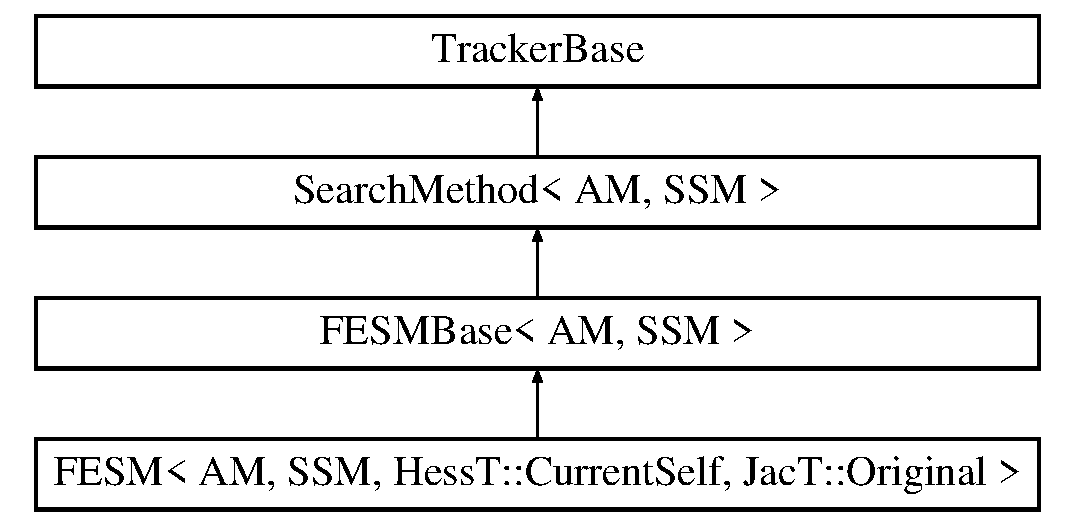
\includegraphics[height=4.000000cm]{classFESM_3_01AM_00_01SSM_00_01HessT_1_1CurrentSelf_00_01JacT_1_1Original_01_4}
\end{center}
\end{figure}
\subsection*{Additional Inherited Members}


The documentation for this class was generated from the following file\-:\begin{DoxyCompactItemize}
\item 
S\-M/include/mtf/\-S\-M/F\-E\-S\-M.\-h\end{DoxyCompactItemize}

\hypertarget{classFESM_3_01AM_00_01SSM_00_01HessT_1_1InitialSelf_00_01JacT_1_1DiffOfJacs_01_4}{\section{F\-E\-S\-M$<$ A\-M, S\-S\-M, Hess\-T\-:\-:Initial\-Self, Jac\-T\-:\-:Diff\-Of\-Jacs $>$ Class Template Reference}
\label{classFESM_3_01AM_00_01SSM_00_01HessT_1_1InitialSelf_00_01JacT_1_1DiffOfJacs_01_4}\index{F\-E\-S\-M$<$ A\-M, S\-S\-M, Hess\-T\-::\-Initial\-Self, Jac\-T\-::\-Diff\-Of\-Jacs $>$@{F\-E\-S\-M$<$ A\-M, S\-S\-M, Hess\-T\-::\-Initial\-Self, Jac\-T\-::\-Diff\-Of\-Jacs $>$}}
}
Inheritance diagram for F\-E\-S\-M$<$ A\-M, S\-S\-M, Hess\-T\-:\-:Initial\-Self, Jac\-T\-:\-:Diff\-Of\-Jacs $>$\-:\begin{figure}[H]
\begin{center}
\leavevmode
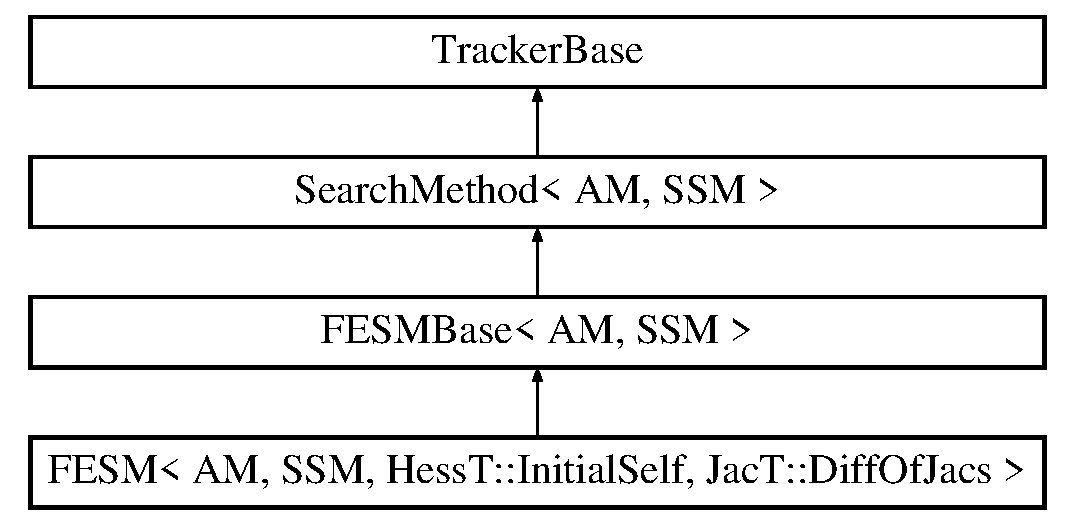
\includegraphics[height=4.000000cm]{classFESM_3_01AM_00_01SSM_00_01HessT_1_1InitialSelf_00_01JacT_1_1DiffOfJacs_01_4}
\end{center}
\end{figure}
\subsection*{Additional Inherited Members}


The documentation for this class was generated from the following file\-:\begin{DoxyCompactItemize}
\item 
S\-M/include/mtf/\-S\-M/F\-E\-S\-M.\-h\end{DoxyCompactItemize}

\hypertarget{classFESM_3_01AM_00_01SSM_00_01HessT_1_1InitialSelf_00_01JacT_1_1Original_01_4}{\section{F\-E\-S\-M$<$ A\-M, S\-S\-M, Hess\-T\-:\-:Initial\-Self, Jac\-T\-:\-:Original $>$ Class Template Reference}
\label{classFESM_3_01AM_00_01SSM_00_01HessT_1_1InitialSelf_00_01JacT_1_1Original_01_4}\index{F\-E\-S\-M$<$ A\-M, S\-S\-M, Hess\-T\-::\-Initial\-Self, Jac\-T\-::\-Original $>$@{F\-E\-S\-M$<$ A\-M, S\-S\-M, Hess\-T\-::\-Initial\-Self, Jac\-T\-::\-Original $>$}}
}
Inheritance diagram for F\-E\-S\-M$<$ A\-M, S\-S\-M, Hess\-T\-:\-:Initial\-Self, Jac\-T\-:\-:Original $>$\-:\begin{figure}[H]
\begin{center}
\leavevmode
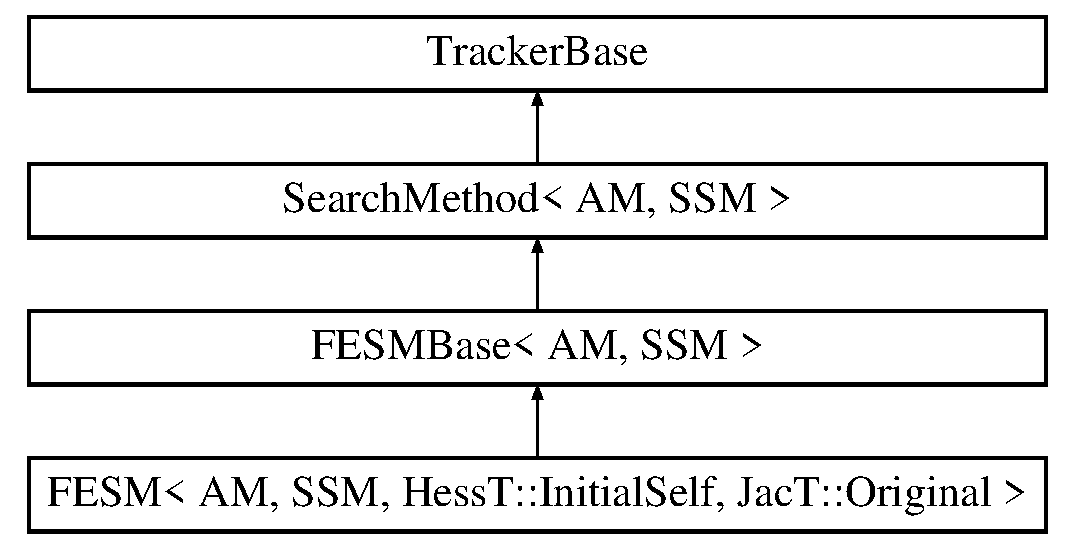
\includegraphics[height=4.000000cm]{classFESM_3_01AM_00_01SSM_00_01HessT_1_1InitialSelf_00_01JacT_1_1Original_01_4}
\end{center}
\end{figure}
\subsection*{Additional Inherited Members}


The documentation for this class was generated from the following file\-:\begin{DoxyCompactItemize}
\item 
S\-M/include/mtf/\-S\-M/F\-E\-S\-M.\-h\end{DoxyCompactItemize}

\hypertarget{classFESM_3_01AM_00_01SSM_00_01HessT_1_1Original_00_01JacT_1_1DiffOfJacs_01_4}{\section{F\-E\-S\-M$<$ A\-M, S\-S\-M, Hess\-T\-:\-:Original, Jac\-T\-:\-:Diff\-Of\-Jacs $>$ Class Template Reference}
\label{classFESM_3_01AM_00_01SSM_00_01HessT_1_1Original_00_01JacT_1_1DiffOfJacs_01_4}\index{F\-E\-S\-M$<$ A\-M, S\-S\-M, Hess\-T\-::\-Original, Jac\-T\-::\-Diff\-Of\-Jacs $>$@{F\-E\-S\-M$<$ A\-M, S\-S\-M, Hess\-T\-::\-Original, Jac\-T\-::\-Diff\-Of\-Jacs $>$}}
}
Inheritance diagram for F\-E\-S\-M$<$ A\-M, S\-S\-M, Hess\-T\-:\-:Original, Jac\-T\-:\-:Diff\-Of\-Jacs $>$\-:\begin{figure}[H]
\begin{center}
\leavevmode
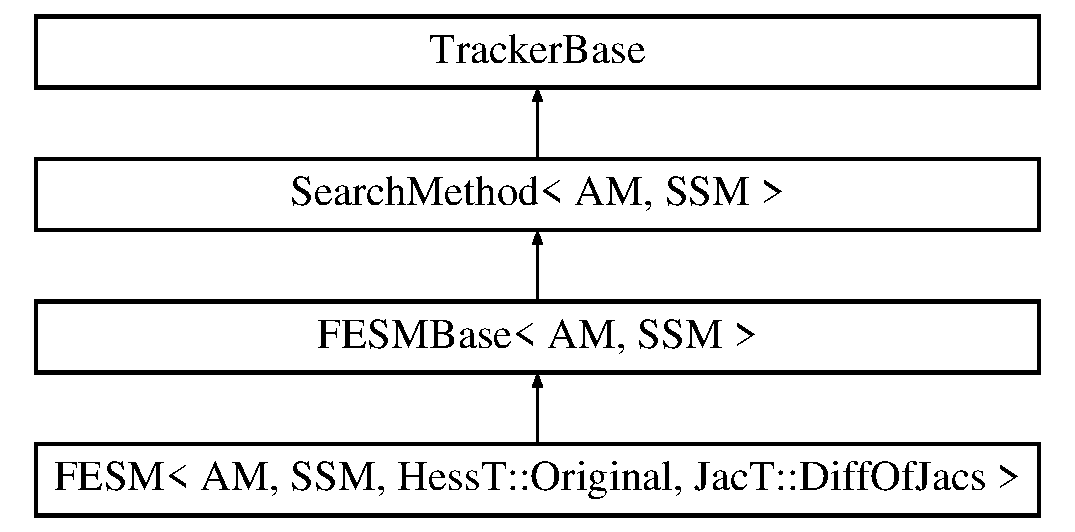
\includegraphics[height=4.000000cm]{classFESM_3_01AM_00_01SSM_00_01HessT_1_1Original_00_01JacT_1_1DiffOfJacs_01_4}
\end{center}
\end{figure}
\subsection*{Additional Inherited Members}


The documentation for this class was generated from the following file\-:\begin{DoxyCompactItemize}
\item 
S\-M/include/mtf/\-S\-M/F\-E\-S\-M.\-h\end{DoxyCompactItemize}

\hypertarget{classFESM_3_01AM_00_01SSM_00_01HessT_1_1Original_00_01JacT_1_1Original_01_4}{\section{F\-E\-S\-M$<$ A\-M, S\-S\-M, Hess\-T\-:\-:Original, Jac\-T\-:\-:Original $>$ Class Template Reference}
\label{classFESM_3_01AM_00_01SSM_00_01HessT_1_1Original_00_01JacT_1_1Original_01_4}\index{F\-E\-S\-M$<$ A\-M, S\-S\-M, Hess\-T\-::\-Original, Jac\-T\-::\-Original $>$@{F\-E\-S\-M$<$ A\-M, S\-S\-M, Hess\-T\-::\-Original, Jac\-T\-::\-Original $>$}}
}
Inheritance diagram for F\-E\-S\-M$<$ A\-M, S\-S\-M, Hess\-T\-:\-:Original, Jac\-T\-:\-:Original $>$\-:\begin{figure}[H]
\begin{center}
\leavevmode
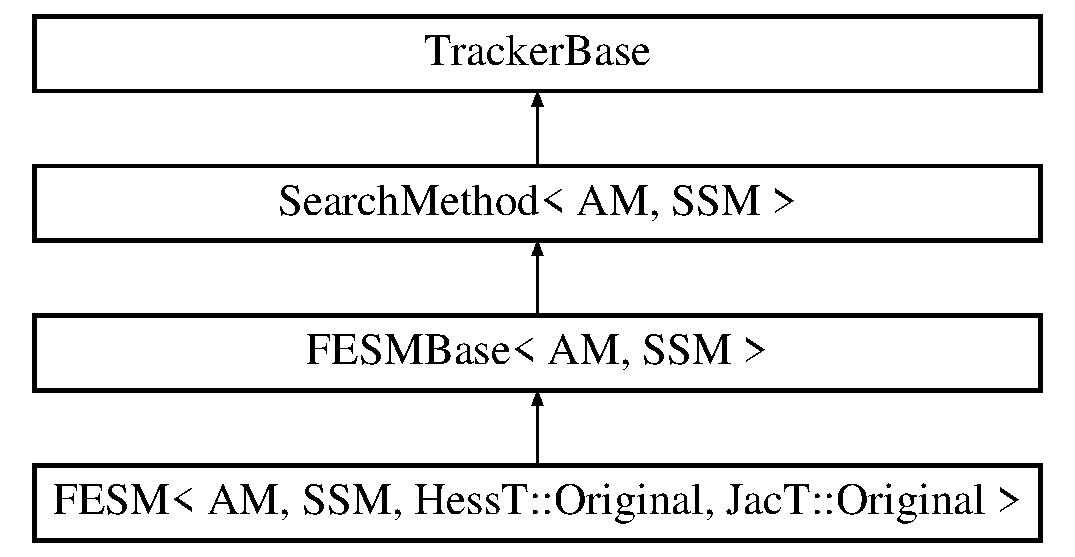
\includegraphics[height=4.000000cm]{classFESM_3_01AM_00_01SSM_00_01HessT_1_1Original_00_01JacT_1_1Original_01_4}
\end{center}
\end{figure}
\subsection*{Additional Inherited Members}


The documentation for this class was generated from the following file\-:\begin{DoxyCompactItemize}
\item 
S\-M/include/mtf/\-S\-M/F\-E\-S\-M.\-h\end{DoxyCompactItemize}

\hypertarget{classFESM_3_01AM_00_01SSM_00_01HessT_1_1Std_00_01JacT_1_1DiffOfJacs_01_4}{\section{F\-E\-S\-M$<$ A\-M, S\-S\-M, Hess\-T\-:\-:Std, Jac\-T\-:\-:Diff\-Of\-Jacs $>$ Class Template Reference}
\label{classFESM_3_01AM_00_01SSM_00_01HessT_1_1Std_00_01JacT_1_1DiffOfJacs_01_4}\index{F\-E\-S\-M$<$ A\-M, S\-S\-M, Hess\-T\-::\-Std, Jac\-T\-::\-Diff\-Of\-Jacs $>$@{F\-E\-S\-M$<$ A\-M, S\-S\-M, Hess\-T\-::\-Std, Jac\-T\-::\-Diff\-Of\-Jacs $>$}}
}
Inheritance diagram for F\-E\-S\-M$<$ A\-M, S\-S\-M, Hess\-T\-:\-:Std, Jac\-T\-:\-:Diff\-Of\-Jacs $>$\-:\begin{figure}[H]
\begin{center}
\leavevmode
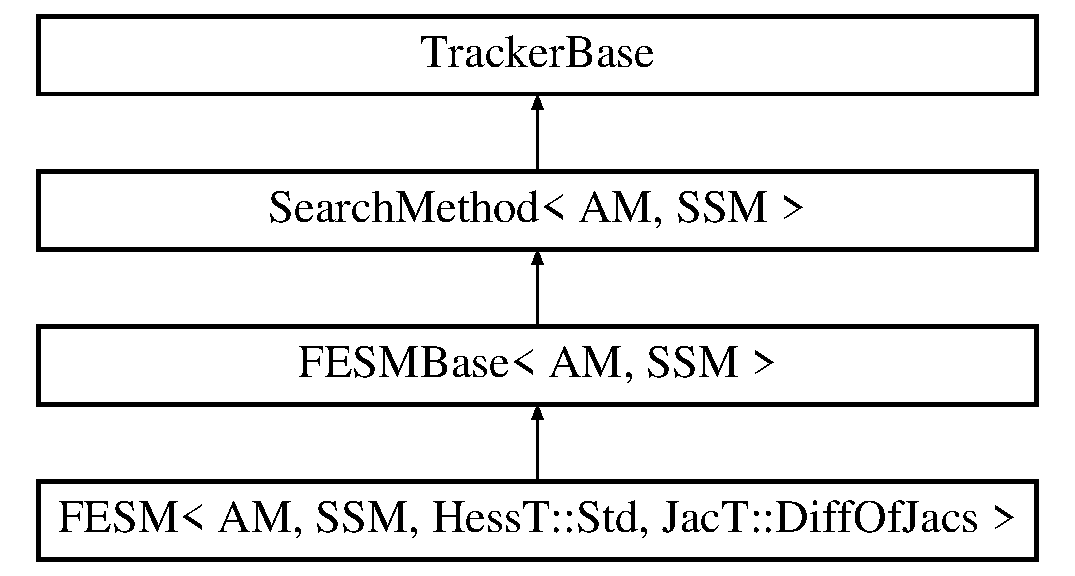
\includegraphics[height=4.000000cm]{classFESM_3_01AM_00_01SSM_00_01HessT_1_1Std_00_01JacT_1_1DiffOfJacs_01_4}
\end{center}
\end{figure}
\subsection*{Additional Inherited Members}


The documentation for this class was generated from the following file\-:\begin{DoxyCompactItemize}
\item 
S\-M/include/mtf/\-S\-M/F\-E\-S\-M.\-h\end{DoxyCompactItemize}

\hypertarget{classFESM_3_01AM_00_01SSM_00_01HessT_1_1Std_00_01JacT_1_1Original_01_4}{\section{F\-E\-S\-M$<$ A\-M, S\-S\-M, Hess\-T\-:\-:Std, Jac\-T\-:\-:Original $>$ Class Template Reference}
\label{classFESM_3_01AM_00_01SSM_00_01HessT_1_1Std_00_01JacT_1_1Original_01_4}\index{F\-E\-S\-M$<$ A\-M, S\-S\-M, Hess\-T\-::\-Std, Jac\-T\-::\-Original $>$@{F\-E\-S\-M$<$ A\-M, S\-S\-M, Hess\-T\-::\-Std, Jac\-T\-::\-Original $>$}}
}
Inheritance diagram for F\-E\-S\-M$<$ A\-M, S\-S\-M, Hess\-T\-:\-:Std, Jac\-T\-:\-:Original $>$\-:\begin{figure}[H]
\begin{center}
\leavevmode
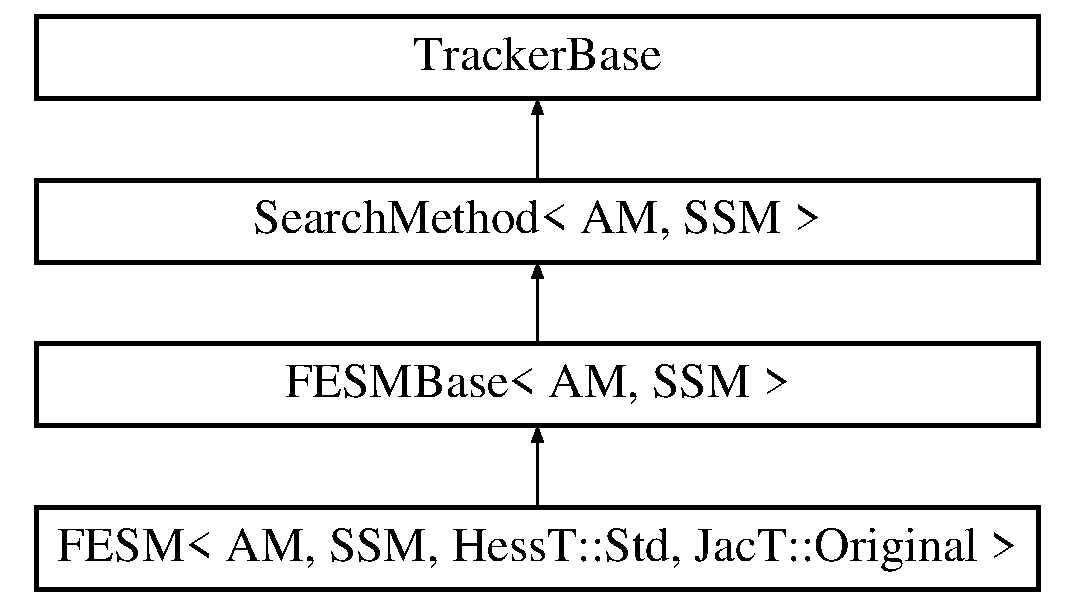
\includegraphics[height=4.000000cm]{classFESM_3_01AM_00_01SSM_00_01HessT_1_1Std_00_01JacT_1_1Original_01_4}
\end{center}
\end{figure}
\subsection*{Additional Inherited Members}


The documentation for this class was generated from the following file\-:\begin{DoxyCompactItemize}
\item 
S\-M/include/mtf/\-S\-M/F\-E\-S\-M.\-h\end{DoxyCompactItemize}

\hypertarget{classFESM_3_01AM_00_01SSM_00_01HessT_1_1SumOfSelf_00_01JacT_1_1DiffOfJacs_01_4}{\section{F\-E\-S\-M$<$ A\-M, S\-S\-M, Hess\-T\-:\-:Sum\-Of\-Self, Jac\-T\-:\-:Diff\-Of\-Jacs $>$ Class Template Reference}
\label{classFESM_3_01AM_00_01SSM_00_01HessT_1_1SumOfSelf_00_01JacT_1_1DiffOfJacs_01_4}\index{F\-E\-S\-M$<$ A\-M, S\-S\-M, Hess\-T\-::\-Sum\-Of\-Self, Jac\-T\-::\-Diff\-Of\-Jacs $>$@{F\-E\-S\-M$<$ A\-M, S\-S\-M, Hess\-T\-::\-Sum\-Of\-Self, Jac\-T\-::\-Diff\-Of\-Jacs $>$}}
}
Inheritance diagram for F\-E\-S\-M$<$ A\-M, S\-S\-M, Hess\-T\-:\-:Sum\-Of\-Self, Jac\-T\-:\-:Diff\-Of\-Jacs $>$\-:\begin{figure}[H]
\begin{center}
\leavevmode
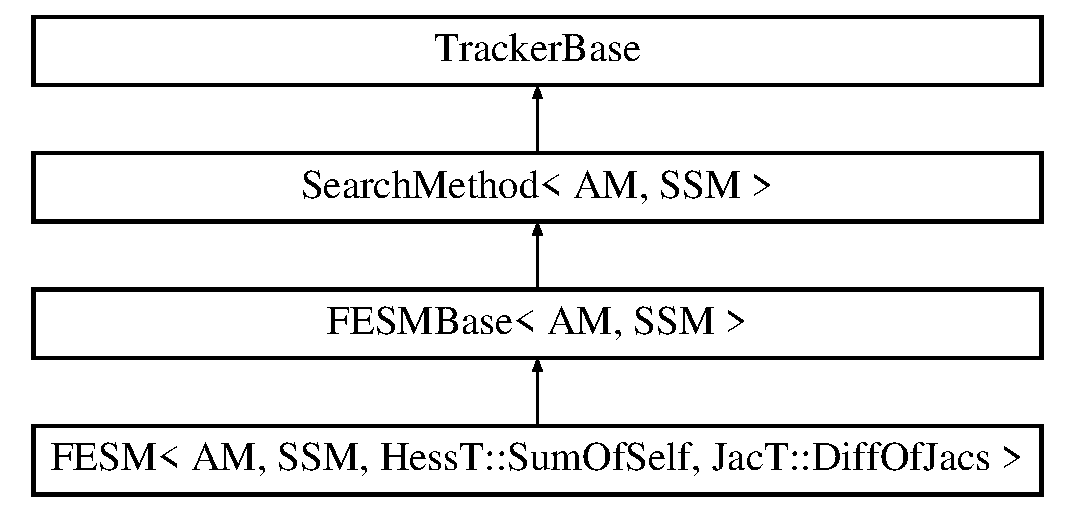
\includegraphics[height=4.000000cm]{classFESM_3_01AM_00_01SSM_00_01HessT_1_1SumOfSelf_00_01JacT_1_1DiffOfJacs_01_4}
\end{center}
\end{figure}
\subsection*{Additional Inherited Members}


The documentation for this class was generated from the following file\-:\begin{DoxyCompactItemize}
\item 
S\-M/include/mtf/\-S\-M/F\-E\-S\-M.\-h\end{DoxyCompactItemize}

\hypertarget{classFESM_3_01AM_00_01SSM_00_01HessT_1_1SumOfSelf_00_01JacT_1_1Original_01_4}{\section{F\-E\-S\-M$<$ A\-M, S\-S\-M, Hess\-T\-:\-:Sum\-Of\-Self, Jac\-T\-:\-:Original $>$ Class Template Reference}
\label{classFESM_3_01AM_00_01SSM_00_01HessT_1_1SumOfSelf_00_01JacT_1_1Original_01_4}\index{F\-E\-S\-M$<$ A\-M, S\-S\-M, Hess\-T\-::\-Sum\-Of\-Self, Jac\-T\-::\-Original $>$@{F\-E\-S\-M$<$ A\-M, S\-S\-M, Hess\-T\-::\-Sum\-Of\-Self, Jac\-T\-::\-Original $>$}}
}
Inheritance diagram for F\-E\-S\-M$<$ A\-M, S\-S\-M, Hess\-T\-:\-:Sum\-Of\-Self, Jac\-T\-:\-:Original $>$\-:\begin{figure}[H]
\begin{center}
\leavevmode
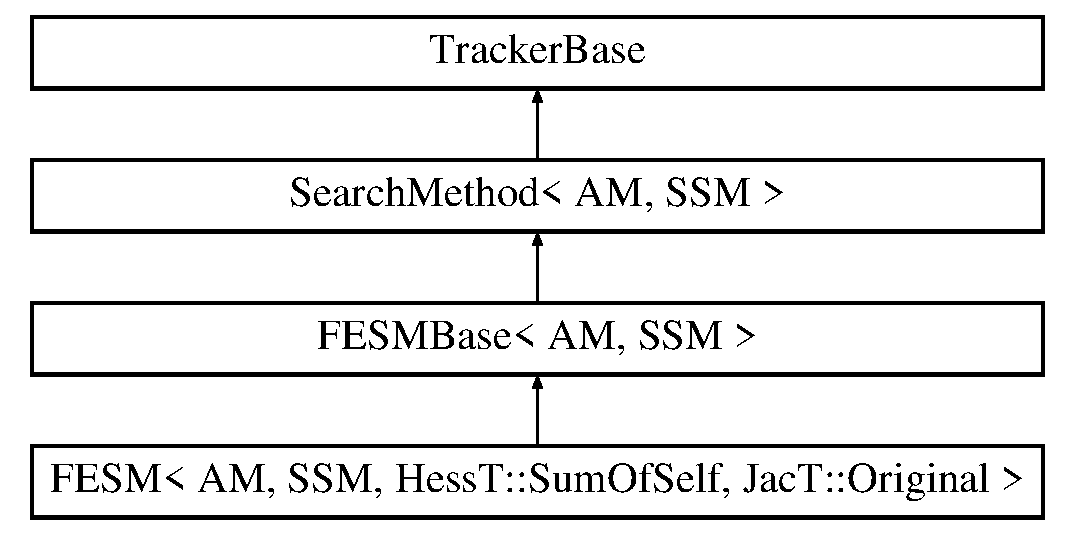
\includegraphics[height=4.000000cm]{classFESM_3_01AM_00_01SSM_00_01HessT_1_1SumOfSelf_00_01JacT_1_1Original_01_4}
\end{center}
\end{figure}
\subsection*{Additional Inherited Members}


The documentation for this class was generated from the following file\-:\begin{DoxyCompactItemize}
\item 
S\-M/include/mtf/\-S\-M/F\-E\-S\-M.\-h\end{DoxyCompactItemize}

\hypertarget{classFESM_3_01AM_00_01SSM_00_01HessT_1_1SumOfStd_00_01JacT_1_1DiffOfJacs_01_4}{\section{F\-E\-S\-M$<$ A\-M, S\-S\-M, Hess\-T\-:\-:Sum\-Of\-Std, Jac\-T\-:\-:Diff\-Of\-Jacs $>$ Class Template Reference}
\label{classFESM_3_01AM_00_01SSM_00_01HessT_1_1SumOfStd_00_01JacT_1_1DiffOfJacs_01_4}\index{F\-E\-S\-M$<$ A\-M, S\-S\-M, Hess\-T\-::\-Sum\-Of\-Std, Jac\-T\-::\-Diff\-Of\-Jacs $>$@{F\-E\-S\-M$<$ A\-M, S\-S\-M, Hess\-T\-::\-Sum\-Of\-Std, Jac\-T\-::\-Diff\-Of\-Jacs $>$}}
}
Inheritance diagram for F\-E\-S\-M$<$ A\-M, S\-S\-M, Hess\-T\-:\-:Sum\-Of\-Std, Jac\-T\-:\-:Diff\-Of\-Jacs $>$\-:\begin{figure}[H]
\begin{center}
\leavevmode
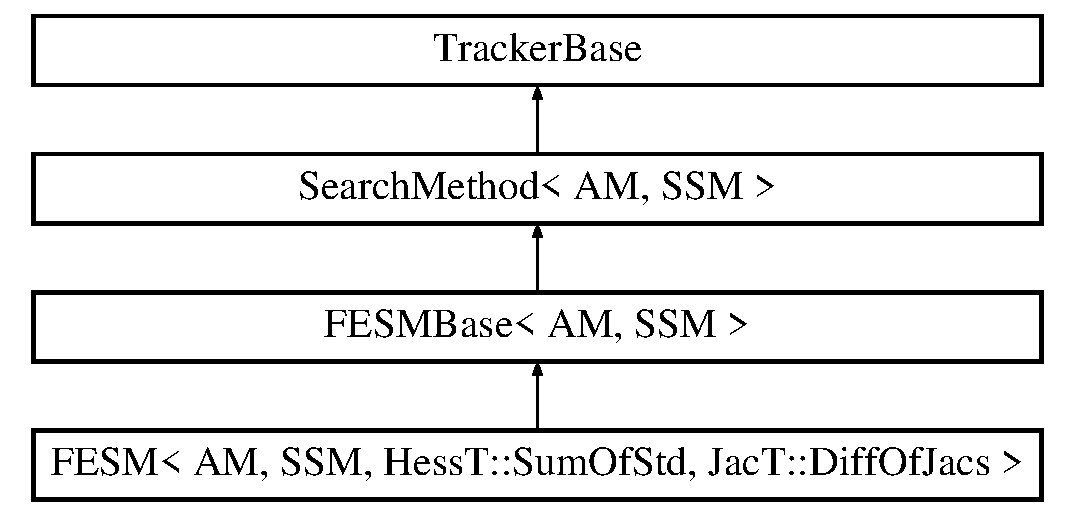
\includegraphics[height=4.000000cm]{classFESM_3_01AM_00_01SSM_00_01HessT_1_1SumOfStd_00_01JacT_1_1DiffOfJacs_01_4}
\end{center}
\end{figure}
\subsection*{Additional Inherited Members}


The documentation for this class was generated from the following file\-:\begin{DoxyCompactItemize}
\item 
S\-M/include/mtf/\-S\-M/F\-E\-S\-M.\-h\end{DoxyCompactItemize}

\hypertarget{classFESM_3_01AM_00_01SSM_00_01HessT_1_1SumOfStd_00_01JacT_1_1Original_01_4}{\section{F\-E\-S\-M$<$ A\-M, S\-S\-M, Hess\-T\-:\-:Sum\-Of\-Std, Jac\-T\-:\-:Original $>$ Class Template Reference}
\label{classFESM_3_01AM_00_01SSM_00_01HessT_1_1SumOfStd_00_01JacT_1_1Original_01_4}\index{F\-E\-S\-M$<$ A\-M, S\-S\-M, Hess\-T\-::\-Sum\-Of\-Std, Jac\-T\-::\-Original $>$@{F\-E\-S\-M$<$ A\-M, S\-S\-M, Hess\-T\-::\-Sum\-Of\-Std, Jac\-T\-::\-Original $>$}}
}
Inheritance diagram for F\-E\-S\-M$<$ A\-M, S\-S\-M, Hess\-T\-:\-:Sum\-Of\-Std, Jac\-T\-:\-:Original $>$\-:\begin{figure}[H]
\begin{center}
\leavevmode
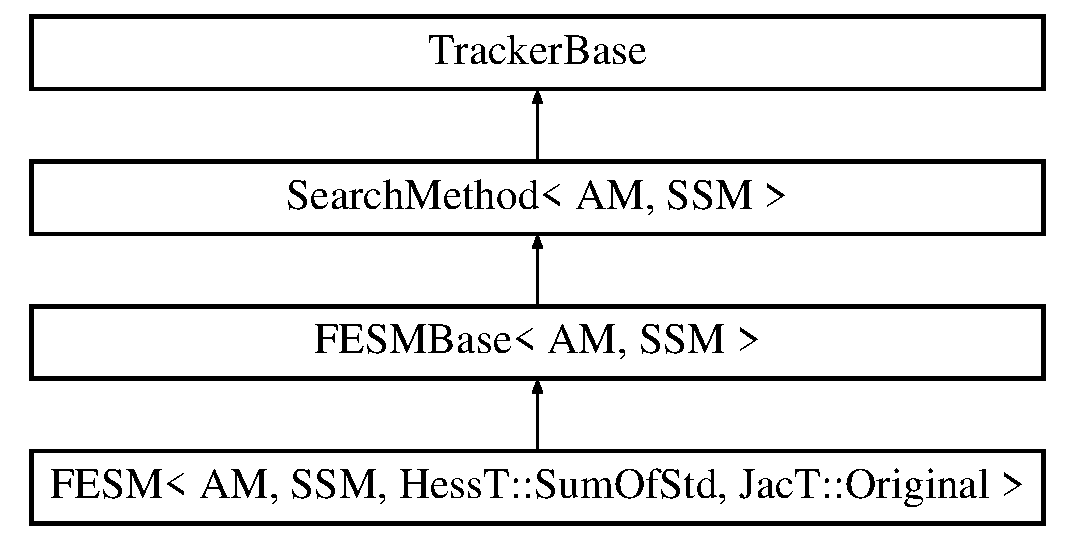
\includegraphics[height=4.000000cm]{classFESM_3_01AM_00_01SSM_00_01HessT_1_1SumOfStd_00_01JacT_1_1Original_01_4}
\end{center}
\end{figure}
\subsection*{Additional Inherited Members}


The documentation for this class was generated from the following file\-:\begin{DoxyCompactItemize}
\item 
S\-M/include/mtf/\-S\-M/F\-E\-S\-M.\-h\end{DoxyCompactItemize}

\hypertarget{classFESMBase}{\section{F\-E\-S\-M\-Base$<$ A\-M, S\-S\-M $>$ Class Template Reference}
\label{classFESMBase}\index{F\-E\-S\-M\-Base$<$ A\-M, S\-S\-M $>$@{F\-E\-S\-M\-Base$<$ A\-M, S\-S\-M $>$}}
}
Inheritance diagram for F\-E\-S\-M\-Base$<$ A\-M, S\-S\-M $>$\-:\begin{figure}[H]
\begin{center}
\leavevmode
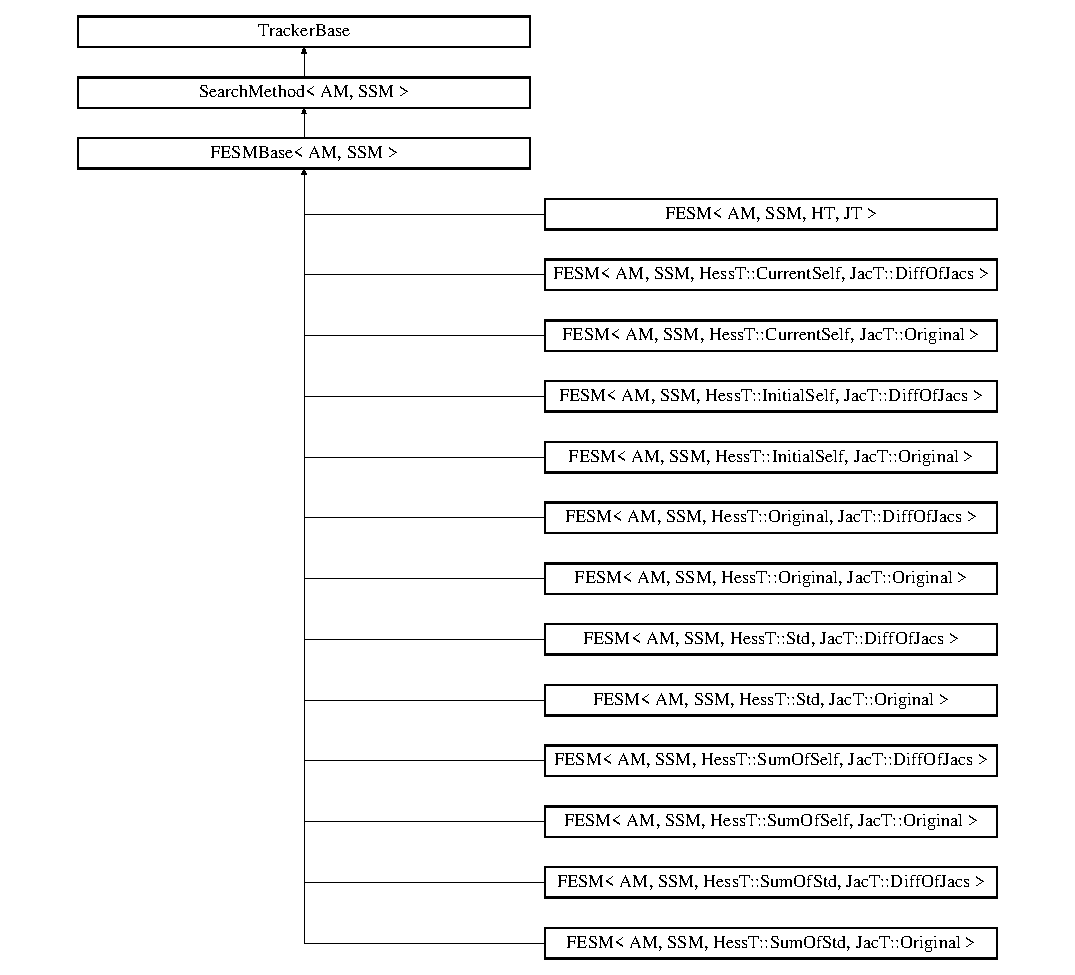
\includegraphics[height=12.000000cm]{classFESMBase}
\end{center}
\end{figure}
\subsection*{Public Types}
\begin{DoxyCompactItemize}
\item 
\hypertarget{classFESMBase_a3381cf9dd84b83d8c25206899608df05}{typedef \hyperlink{structFESMParams}{F\-E\-S\-M\-Params} {\bfseries Param\-Type}}\label{classFESMBase_a3381cf9dd84b83d8c25206899608df05}

\end{DoxyCompactItemize}
\subsection*{Public Member Functions}
\begin{DoxyCompactItemize}
\item 
\hypertarget{classFESMBase_a6359268e77e5281e263bceec2aa72a30}{{\bfseries F\-E\-S\-M\-Base} (const \hyperlink{structFESMParams}{Param\-Type} $\ast$nesm\-\_\-params=nullptr, const \hyperlink{structAMParams}{A\-M\-Params} $\ast$am\-\_\-params=nullptr, const \hyperlink{structSSMParams}{S\-S\-M\-Params} $\ast$ssm\-\_\-params=nullptr)}\label{classFESMBase_a6359268e77e5281e263bceec2aa72a30}

\item 
\hypertarget{classFESMBase_a8f33c0a97b770ab8c94a18232cfed36b}{void {\bfseries initialize} (const cv\-::\-Mat \&corners) override}\label{classFESMBase_a8f33c0a97b770ab8c94a18232cfed36b}

\item 
\hypertarget{classFESMBase_a49434680fff2e8dc565c635509a37c8a}{void {\bfseries update} () override}\label{classFESMBase_a49434680fff2e8dc565c635509a37c8a}

\item 
\hypertarget{classFESMBase_a0281092da8951b938e6e08e413d8dd95}{virtual void {\bfseries initialize\-Hessian} ()}\label{classFESMBase_a0281092da8951b938e6e08e413d8dd95}

\item 
\hypertarget{classFESMBase_ac67403ec83a42647444af782c6b3f5e6}{virtual void {\bfseries update\-Jacobian} ()}\label{classFESMBase_ac67403ec83a42647444af782c6b3f5e6}

\item 
\hypertarget{classFESMBase_ac1ae6ee31d41ae60419cdc8523d93da8}{virtual void {\bfseries update\-Hessian} ()}\label{classFESMBase_ac1ae6ee31d41ae60419cdc8523d93da8}

\item 
\hypertarget{classFESMBase_a7b3bc0abeb9ee2a5488c637f3abe03dd}{void {\bfseries initialize\-Pix\-Jacobian} ()}\label{classFESMBase_a7b3bc0abeb9ee2a5488c637f3abe03dd}

\item 
\hypertarget{classFESMBase_a72237505f86f83ca2a35a44035f5e9ab}{void {\bfseries update\-Pix\-Jacobian} ()}\label{classFESMBase_a72237505f86f83ca2a35a44035f5e9ab}

\item 
\hypertarget{classFESMBase_ad131b772b18b8a56c4069273d6b3a9e7}{void {\bfseries initialize\-Pix\-Hessian} ()}\label{classFESMBase_ad131b772b18b8a56c4069273d6b3a9e7}

\item 
\hypertarget{classFESMBase_a753139af0c519cb5dd0eeb665351bfc6}{void {\bfseries update\-Pix\-Hessian} ()}\label{classFESMBase_a753139af0c519cb5dd0eeb665351bfc6}

\item 
\hypertarget{classFESMBase_a93e4cd5795659c69f782bd96fd71d2e1}{void {\bfseries update\-S\-S\-M} ()}\label{classFESMBase_a93e4cd5795659c69f782bd96fd71d2e1}

\end{DoxyCompactItemize}
\subsection*{Public Attributes}
\begin{DoxyCompactItemize}
\item 
\hypertarget{classFESMBase_ad833897d1bda90e59209b474bdb0cdf6}{\hyperlink{structFESMParams}{Param\-Type} {\bfseries params}}\label{classFESMBase_ad833897d1bda90e59209b474bdb0cdf6}

\item 
\hypertarget{classFESMBase_a644eb5767a50e0620844201fbee77d63}{int {\bfseries frame\-\_\-id}}\label{classFESMBase_a644eb5767a50e0620844201fbee77d63}

\item 
\hypertarget{classFESMBase_a173bb869a75c3871003a49bde1f143cb}{Vector\-Xc {\bfseries pix\-\_\-mask2}}\label{classFESMBase_a173bb869a75c3871003a49bde1f143cb}

\item 
\hypertarget{classFESMBase_a39da3447ecd99fa16fedd103260d1043}{Vector\-Xb {\bfseries pix\-\_\-mask}}\label{classFESMBase_a39da3447ecd99fa16fedd103260d1043}

\item 
\hypertarget{classFESMBase_ae1d98232c2b4d658cdd4424504165b00}{Vector\-Xd {\bfseries rel\-\_\-pix\-\_\-diff}}\label{classFESMBase_ae1d98232c2b4d658cdd4424504165b00}

\item 
\hypertarget{classFESMBase_a1f0a176d87626f95609427a346c009c0}{cv\-::\-Mat {\bfseries pix\-\_\-mask\-\_\-img}}\label{classFESMBase_a1f0a176d87626f95609427a346c009c0}

\item 
\hypertarget{classFESMBase_a1ae62610166d11e22e1c2895d03e5e1c}{double {\bfseries max\-\_\-pix\-\_\-diff}}\label{classFESMBase_a1ae62610166d11e22e1c2895d03e5e1c}

\item 
\hypertarget{classFESMBase_a15411a400a6c5dd4c3b3b46c3b2a02d9}{char $\ast$ {\bfseries spi\-\_\-win\-\_\-name}}\label{classFESMBase_a15411a400a6c5dd4c3b3b46c3b2a02d9}

\item 
\hypertarget{classFESMBase_a2c6a93ada38a61c26115942ed145b63c}{Matrix24d {\bfseries prev\-\_\-corners}}\label{classFESMBase_a2c6a93ada38a61c26115942ed145b63c}

\item 
Matrix\-Xd \hyperlink{classFESMBase_a34b1dddc4fb6e3f4187e0388cb8684f2}{init\-\_\-pix\-\_\-jacobian}
\begin{DoxyCompactList}\small\item\em N x S jacobians of the pixel values w.\-r.\-t the S\-S\-M state vector where N = resx $\ast$ resy is the no. \end{DoxyCompactList}\item 
\hypertarget{classFESMBase_ad4c68c2bd2d2681e17ac78e7a4a6fe21}{Matrix\-Xd {\bfseries curr\-\_\-pix\-\_\-jacobian}}\label{classFESMBase_ad4c68c2bd2d2681e17ac78e7a4a6fe21}

\item 
\hypertarget{classFESMBase_a54cf375ad07c991639e704dd964b9dd7}{Matrix\-Xd {\bfseries mean\-\_\-pix\-\_\-jacobian}}\label{classFESMBase_a54cf375ad07c991639e704dd964b9dd7}

\item 
\hypertarget{classFESMBase_a82cc6779a62c119303e6c238a81c9086}{Matrix\-Xd {\bfseries init\-\_\-pix\-\_\-hessian}}\label{classFESMBase_a82cc6779a62c119303e6c238a81c9086}

\item 
\hypertarget{classFESMBase_a82b55b9e1a56ef8139001ee56b0aacbf}{Matrix\-Xd {\bfseries curr\-\_\-pix\-\_\-hessian}}\label{classFESMBase_a82b55b9e1a56ef8139001ee56b0aacbf}

\item 
\hypertarget{classFESMBase_a6118749603515af235660ebcb48b8bc2}{Matrix\-Xd {\bfseries mean\-\_\-pix\-\_\-hessian}}\label{classFESMBase_a6118749603515af235660ebcb48b8bc2}

\item 
\hypertarget{classFESMBase_a9b101a654808d0eba20b501926852821}{Vector\-Xd {\bfseries ssm\-\_\-update}}\label{classFESMBase_a9b101a654808d0eba20b501926852821}

\item 
\hypertarget{classFESMBase_a393cd49f14c35b7c76b5f53e8c5ae216}{Row\-Vector\-Xd \hyperlink{classFESMBase_a393cd49f14c35b7c76b5f53e8c5ae216}{jacobian}}\label{classFESMBase_a393cd49f14c35b7c76b5f53e8c5ae216}

\begin{DoxyCompactList}\small\item\em 1 x S Jacobian of the A\-M error norm w.\-r.\-t. S\-S\-M state vector \end{DoxyCompactList}\item 
\hypertarget{classFESMBase_ab19e7ff8aab8aa8267e5b3e77ba83387}{Matrix\-Xd \hyperlink{classFESMBase_ab19e7ff8aab8aa8267e5b3e77ba83387}{hessian}}\label{classFESMBase_ab19e7ff8aab8aa8267e5b3e77ba83387}

\begin{DoxyCompactList}\small\item\em S x S Hessian of the A\-M error norm w.\-r.\-t. S\-S\-M state vector. \end{DoxyCompactList}\item 
\hypertarget{classFESMBase_ae23df79dd448c828a20be7a80ead0acc}{Matrix\-Xd {\bfseries init\-\_\-self\-\_\-hessian}}\label{classFESMBase_ae23df79dd448c828a20be7a80ead0acc}

\end{DoxyCompactItemize}
\subsection*{Protected Member Functions}
\begin{DoxyCompactItemize}
\item 
\hypertarget{classFESMBase_a07512215cb0766f232ec1dd0fa6624a2}{{\bfseries init\-\_\-profiling} ()}\label{classFESMBase_a07512215cb0766f232ec1dd0fa6624a2}

\item 
\hypertarget{classFESMBase_af63d3fae8a50100dd88cdc935bbfed46}{void {\bfseries initialize\-S\-P\-I\-Mask} ()}\label{classFESMBase_af63d3fae8a50100dd88cdc935bbfed46}

\item 
\hypertarget{classFESMBase_aa6c5a95dae5b3aaec9c2109fc07686dd}{void {\bfseries update\-S\-P\-I\-Mask} ()}\label{classFESMBase_aa6c5a95dae5b3aaec9c2109fc07686dd}

\item 
\hypertarget{classFESMBase_af3b8ecbd65a5e067300a2aa4b61d4c38}{void {\bfseries show\-S\-P\-I\-Mask} ()}\label{classFESMBase_af3b8ecbd65a5e067300a2aa4b61d4c38}

\end{DoxyCompactItemize}
\subsection*{Protected Attributes}
\begin{DoxyCompactItemize}
\item 
\hypertarget{classFESMBase_a0f57bb400abbe8f35c0f683e19f96047}{char $\ast$ {\bfseries time\-\_\-fname}}\label{classFESMBase_a0f57bb400abbe8f35c0f683e19f96047}

\item 
\hypertarget{classFESMBase_aa8dead227cd5528f35a6db3485db062d}{char $\ast$ {\bfseries log\-\_\-fname}}\label{classFESMBase_aa8dead227cd5528f35a6db3485db062d}

\item 
\hypertarget{classFESMBase_a4689d0be67145da047e2c32f0cdf303f}{string {\bfseries hess\-\_\-order}}\label{classFESMBase_a4689d0be67145da047e2c32f0cdf303f}

\end{DoxyCompactItemize}


\subsection{Member Data Documentation}
\hypertarget{classFESMBase_a34b1dddc4fb6e3f4187e0388cb8684f2}{\index{F\-E\-S\-M\-Base@{F\-E\-S\-M\-Base}!init\-\_\-pix\-\_\-jacobian@{init\-\_\-pix\-\_\-jacobian}}
\index{init\-\_\-pix\-\_\-jacobian@{init\-\_\-pix\-\_\-jacobian}!FESMBase@{F\-E\-S\-M\-Base}}
\subsubsection[{init\-\_\-pix\-\_\-jacobian}]{\setlength{\rightskip}{0pt plus 5cm}template$<$class A\-M , class S\-S\-M $>$ Matrix\-Xd {\bf F\-E\-S\-M\-Base}$<$ A\-M, S\-S\-M $>$\-::init\-\_\-pix\-\_\-jacobian}}\label{classFESMBase_a34b1dddc4fb6e3f4187e0388cb8684f2}


N x S jacobians of the pixel values w.\-r.\-t the S\-S\-M state vector where N = resx $\ast$ resy is the no. 

of pixels in the object patch 

The documentation for this class was generated from the following file\-:\begin{DoxyCompactItemize}
\item 
S\-M/include/mtf/\-S\-M/F\-E\-S\-M\-Base.\-h\end{DoxyCompactItemize}

\hypertarget{structFESMParams}{\section{F\-E\-S\-M\-Params Struct Reference}
\label{structFESMParams}\index{F\-E\-S\-M\-Params@{F\-E\-S\-M\-Params}}
}
\subsection*{Public Types}
\begin{DoxyCompactItemize}
\item 
enum {\bfseries Jac\-Type} \{ {\bfseries Original}, 
{\bfseries Diff\-Of\-Jacs}
 \}
\item 
enum {\bfseries Hess\-Type} \{ \\*
{\bfseries Original}, 
{\bfseries Sum\-Of\-Std}, 
{\bfseries Sum\-Of\-Self}, 
{\bfseries Initial\-Self}, 
\\*
{\bfseries Current\-Self}, 
{\bfseries Std}
 \}
\end{DoxyCompactItemize}
\subsection*{Public Member Functions}
\begin{DoxyCompactItemize}
\item 
\hyperlink{structFESMParams_a57a82c5ffa65057e1d238ff1854a4c89}{F\-E\-S\-M\-Params} (int \-\_\-max\-\_\-iters, double \-\_\-upd\-\_\-thresh, bool \-\_\-sec\-\_\-ord\-\_\-hess, bool \-\_\-enable\-\_\-spi, double \-\_\-spi\-\_\-thresh, bool \-\_\-debug\-\_\-mode)
\begin{DoxyCompactList}\small\item\em decides whether logging data will be printed for debugging purposes; \end{DoxyCompactList}\item 
\hypertarget{structFESMParams_a3016464835a07fe2813e7ee1bb9e861b}{{\bfseries F\-E\-S\-M\-Params} (\hyperlink{structFESMParams}{F\-E\-S\-M\-Params} $\ast$params=nullptr)}\label{structFESMParams_a3016464835a07fe2813e7ee1bb9e861b}

\end{DoxyCompactItemize}
\subsection*{Public Attributes}
\begin{DoxyCompactItemize}
\item 
\hypertarget{structFESMParams_a96be401b3db2c1b55143dffb8291be20}{int {\bfseries max\-\_\-iters}}\label{structFESMParams_a96be401b3db2c1b55143dffb8291be20}

\item 
\hypertarget{structFESMParams_ad0054f4f49459341a77c51bdce6989d6}{double \hyperlink{structFESMParams_ad0054f4f49459341a77c51bdce6989d6}{upd\-\_\-thresh}}\label{structFESMParams_ad0054f4f49459341a77c51bdce6989d6}

\begin{DoxyCompactList}\small\item\em maximum iterations of the \hyperlink{classFESMBase}{F\-E\-S\-M\-Base} algorithm to run for each frame \end{DoxyCompactList}\item 
\hypertarget{structFESMParams_a24f6ba0bf9d418d9ced7c04f3b4db32a}{bool \hyperlink{structFESMParams_a24f6ba0bf9d418d9ced7c04f3b4db32a}{sec\-\_\-ord\-\_\-hess}}\label{structFESMParams_a24f6ba0bf9d418d9ced7c04f3b4db32a}

\begin{DoxyCompactList}\small\item\em maximum L1 norm of the state update vector at which to stop the iterations \end{DoxyCompactList}\item 
\hypertarget{structFESMParams_a8ade0f5732bcc69614c95898aa2147ad}{bool {\bfseries enable\-\_\-spi}}\label{structFESMParams_a8ade0f5732bcc69614c95898aa2147ad}

\item 
\hypertarget{structFESMParams_a9fadb0002e1632b1c11f302bfd4d6f3a}{double {\bfseries spi\-\_\-thresh}}\label{structFESMParams_a9fadb0002e1632b1c11f302bfd4d6f3a}

\item 
\hypertarget{structFESMParams_a1598fce243fc405685aa6780056ef7f3}{bool {\bfseries debug\-\_\-mode}}\label{structFESMParams_a1598fce243fc405685aa6780056ef7f3}

\end{DoxyCompactItemize}


\subsection{Constructor \& Destructor Documentation}
\hypertarget{structFESMParams_a57a82c5ffa65057e1d238ff1854a4c89}{\index{F\-E\-S\-M\-Params@{F\-E\-S\-M\-Params}!F\-E\-S\-M\-Params@{F\-E\-S\-M\-Params}}
\index{F\-E\-S\-M\-Params@{F\-E\-S\-M\-Params}!FESMParams@{F\-E\-S\-M\-Params}}
\subsubsection[{F\-E\-S\-M\-Params}]{\setlength{\rightskip}{0pt plus 5cm}F\-E\-S\-M\-Params\-::\-F\-E\-S\-M\-Params (
\begin{DoxyParamCaption}
\item[{int}]{\-\_\-max\-\_\-iters, }
\item[{double}]{\-\_\-upd\-\_\-thresh, }
\item[{bool}]{\-\_\-sec\-\_\-ord\-\_\-hess, }
\item[{bool}]{\-\_\-enable\-\_\-spi, }
\item[{double}]{\-\_\-spi\-\_\-thresh, }
\item[{bool}]{\-\_\-debug\-\_\-mode}
\end{DoxyParamCaption}
)\hspace{0.3cm}{\ttfamily [inline]}}}\label{structFESMParams_a57a82c5ffa65057e1d238ff1854a4c89}


decides whether logging data will be printed for debugging purposes; 

only matters if logging is enabled at compile time 

The documentation for this struct was generated from the following file\-:\begin{DoxyCompactItemize}
\item 
S\-M/include/mtf/\-S\-M/F\-E\-S\-M\-Base.\-h\end{DoxyCompactItemize}

\hypertarget{classgnn_1_1FGNN}{\section{gnn\-:\-:F\-G\-N\-N$<$ A\-M $>$ Class Template Reference}
\label{classgnn_1_1FGNN}\index{gnn\-::\-F\-G\-N\-N$<$ A\-M $>$@{gnn\-::\-F\-G\-N\-N$<$ A\-M $>$}}
}
Inheritance diagram for gnn\-:\-:F\-G\-N\-N$<$ A\-M $>$\-:\begin{figure}[H]
\begin{center}
\leavevmode
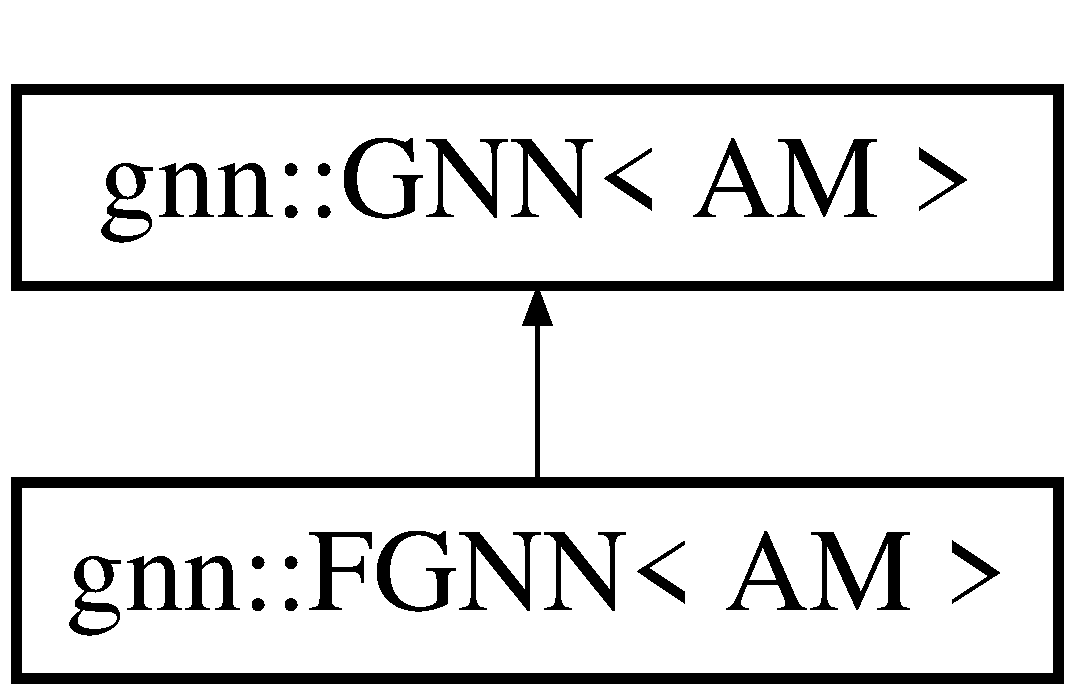
\includegraphics[height=2.000000cm]{classgnn_1_1FGNN}
\end{center}
\end{figure}
\subsection*{Public Types}
\begin{DoxyCompactItemize}
\item 
\hypertarget{classgnn_1_1FGNN_ae5c033a15842672868be407b1a859988}{typedef \hyperlink{classgnn_1_1GNN}{G\-N\-N}$<$ A\-M $>$\-::\hyperlink{structgnn_1_1GNNParams}{Param\-Type} {\bfseries Param\-Type}}\label{classgnn_1_1FGNN_ae5c033a15842672868be407b1a859988}

\item 
\hypertarget{classgnn_1_1FGNN_ae0f5a1e5e0dd1b97a1d2bc93796cd473}{typedef flann\-::\-Matrix$<$ double $>$ {\bfseries flann\-Mat\-T}}\label{classgnn_1_1FGNN_ae0f5a1e5e0dd1b97a1d2bc93796cd473}

\item 
\hypertarget{classgnn_1_1FGNN_aaf008fffa550777666cf892b488ddc53}{typedef flann\-::\-Matrix$<$ int $>$ {\bfseries flann\-Result\-T}}\label{classgnn_1_1FGNN_aaf008fffa550777666cf892b488ddc53}

\item 
\hypertarget{classgnn_1_1FGNN_a1a6bb03c1d1518be57021ef24a92a8ae}{typedef flann\-::\-Index$<$ A\-M $>$ {\bfseries flann\-Idx\-T}}\label{classgnn_1_1FGNN_a1a6bb03c1d1518be57021ef24a92a8ae}

\end{DoxyCompactItemize}
\subsection*{Public Member Functions}
\begin{DoxyCompactItemize}
\item 
\hypertarget{classgnn_1_1FGNN_ae3498d3acfda9c5ddf5b1543a164260e}{{\bfseries F\-G\-N\-N} (const A\-M $\ast$\-\_\-dist\-\_\-func, int \-\_\-n\-\_\-samples, int \-\_\-n\-\_\-dims, bool \-\_\-is\-\_\-symmetrical=true, const \hyperlink{structgnn_1_1GNNParams}{Param\-Type} $\ast$gnn\-\_\-params=nullptr)}\label{classgnn_1_1FGNN_ae3498d3acfda9c5ddf5b1543a164260e}

\item 
\hypertarget{classgnn_1_1FGNN_a091ee7ef53961d0a946fa0fe94954cb9}{void {\bfseries build\-Graph} (const double $\ast$dataset, flann\-Idx\-T $\ast$flann\-\_\-index, const flann\-::\-Search\-Params \&search\-\_\-params)}\label{classgnn_1_1FGNN_a091ee7ef53961d0a946fa0fe94954cb9}

\end{DoxyCompactItemize}
\subsection*{Additional Inherited Members}


The documentation for this class was generated from the following file\-:\begin{DoxyCompactItemize}
\item 
S\-M/include/mtf/\-S\-M/F\-G\-N\-N.\-h\end{DoxyCompactItemize}

\hypertarget{structFLANNParams}{\section{F\-L\-A\-N\-N\-Params Struct Reference}
\label{structFLANNParams}\index{F\-L\-A\-N\-N\-Params@{F\-L\-A\-N\-N\-Params}}
}


index specific params  




{\ttfamily \#include $<$F\-L\-A\-N\-N\-Params.\-h$>$}

\subsection*{Public Types}
\begin{DoxyCompactItemize}
\item 
enum {\bfseries Idx\-Type} \{ \\*
{\bfseries G\-N\-N}, 
{\bfseries K\-D\-Tree}, 
{\bfseries Hierarchical\-Clustering}, 
{\bfseries K\-Means}, 
\\*
{\bfseries Composite}, 
{\bfseries Linear}, 
{\bfseries K\-D\-Tree\-Single}, 
{\bfseries K\-D\-Tree\-Cuda3d}, 
\\*
{\bfseries Autotuned}
 \}
\item 
enum {\bfseries Search\-Type} \{ {\bfseries K\-N\-N}, 
{\bfseries Radius}
 \}
\end{DoxyCompactItemize}
\subsection*{Public Member Functions}
\begin{DoxyCompactItemize}
\item 
\hypertarget{structFLANNParams_af057c64b9666dcfe76b36a35c8767b12}{const flann\-::\-Index\-Params {\bfseries get\-Index\-Params} (Idx\-Type index\-\_\-type, bool load\-\_\-index, std\-::string saved\-\_\-idx\-\_\-path)}\label{structFLANNParams_af057c64b9666dcfe76b36a35c8767b12}

\item 
\hypertarget{structFLANNParams_a76d83b50e5744e1eeb5a2ab2771ed5cb}{void {\bfseries update\-Search\-Params} ()}\label{structFLANNParams_a76d83b50e5744e1eeb5a2ab2771ed5cb}

\item 
\hypertarget{structFLANNParams_acbd7e2aed4b61964b73a6a67a2508a18}{void {\bfseries print\-Params} ()}\label{structFLANNParams_acbd7e2aed4b61964b73a6a67a2508a18}

\item 
\hypertarget{structFLANNParams_a89d32c36efa37f5cf274595609ee4203}{{\bfseries F\-L\-A\-N\-N\-Params} (Search\-Type \-\_\-search\-\_\-type, Idx\-Type \-\_\-index\-\_\-type, Idx\-Type \-\_\-fgnn\-\_\-index\-\_\-type, int \-\_\-srch\-\_\-checks, float \-\_\-srch\-\_\-eps, bool \-\_\-srch\-\_\-sorted, int \-\_\-srch\-\_\-max\-\_\-neighbors, int \-\_\-srch\-\_\-cores, bool \-\_\-srch\-\_\-matrices\-\_\-in\-\_\-gpu\-\_\-ram, flann\-::tri\-\_\-type \-\_\-srch\-\_\-use\-\_\-heap, int kdt\-\_\-trees, int km\-\_\-branching, int km\-\_\-iterations, flann\-::flann\-\_\-centers\-\_\-init\-\_\-t \-\_\-km\-\_\-centers\-\_\-init, float km\-\_\-cb\-\_\-index, int kdts\-\_\-leaf\-\_\-max\-\_\-size, int kdtc\-\_\-leaf\-\_\-max\-\_\-size, int hc\-\_\-branching, flann\-::flann\-\_\-centers\-\_\-init\-\_\-t \-\_\-hc\-\_\-centers\-\_\-init, int hc\-\_\-trees, int hc\-\_\-leaf\-\_\-max\-\_\-size, float auto\-\_\-target\-\_\-precision, float auto\-\_\-build\-\_\-weight, float auto\-\_\-memory\-\_\-weight, float auto\-\_\-sample\-\_\-fraction)}\label{structFLANNParams_a89d32c36efa37f5cf274595609ee4203}

\item 
\hypertarget{structFLANNParams_a7cf9587b5e4aee0dece845dc54ab76f3}{{\bfseries F\-L\-A\-N\-N\-Params} (const \hyperlink{structFLANNParams}{F\-L\-A\-N\-N\-Params} $\ast$params=nullptr)}\label{structFLANNParams_a7cf9587b5e4aee0dece845dc54ab76f3}

\end{DoxyCompactItemize}
\subsection*{Static Public Member Functions}
\begin{DoxyCompactItemize}
\item 
\hypertarget{structFLANNParams_a7d1d264e68d6fbc400a93a2f0f37e08e}{static const char $\ast$ {\bfseries to\-String} (Idx\-Type index\-\_\-type)}\label{structFLANNParams_a7d1d264e68d6fbc400a93a2f0f37e08e}

\item 
\hypertarget{structFLANNParams_adf2cebef4c73ae9a1264feffefb160bd}{static const char $\ast$ {\bfseries to\-String} (Search\-Type index\-\_\-type)}\label{structFLANNParams_adf2cebef4c73ae9a1264feffefb160bd}

\end{DoxyCompactItemize}
\subsection*{Public Attributes}
\begin{DoxyCompactItemize}
\item 
\hypertarget{structFLANNParams_af4e34a5afc91c4695deda58823026890}{flann\-::\-Search\-Params {\bfseries search}}\label{structFLANNParams_af4e34a5afc91c4695deda58823026890}

\item 
\hypertarget{structFLANNParams_ac995a5579a9339682b95931d07fe1eb3}{Search\-Type {\bfseries search\-\_\-type}}\label{structFLANNParams_ac995a5579a9339682b95931d07fe1eb3}

\item 
\hypertarget{structFLANNParams_a99d2e4f15748be233f826958efc87487}{Idx\-Type {\bfseries index\-\_\-type}}\label{structFLANNParams_a99d2e4f15748be233f826958efc87487}

\item 
\hypertarget{structFLANNParams_af8b842b0f8e79ba8d5e34e757b42e6f6}{Idx\-Type {\bfseries fgnn\-\_\-index\-\_\-type}}\label{structFLANNParams_af8b842b0f8e79ba8d5e34e757b42e6f6}

\item 
\hypertarget{structFLANNParams_abcecd1f8b7b38fc91ddc7e0294e423cc}{int {\bfseries srch\-\_\-checks}}\label{structFLANNParams_abcecd1f8b7b38fc91ddc7e0294e423cc}

\item 
\hypertarget{structFLANNParams_aaec471ccff2175ec845d7149cbd81643}{float {\bfseries srch\-\_\-eps}}\label{structFLANNParams_aaec471ccff2175ec845d7149cbd81643}

\item 
\hypertarget{structFLANNParams_ad3eb87a9202039f51b5926c439c9a1e4}{bool {\bfseries srch\-\_\-sorted}}\label{structFLANNParams_ad3eb87a9202039f51b5926c439c9a1e4}

\item 
\hypertarget{structFLANNParams_a034054a451d3adc4b65a7a202b226d0e}{int {\bfseries srch\-\_\-max\-\_\-neighbors}}\label{structFLANNParams_a034054a451d3adc4b65a7a202b226d0e}

\item 
\hypertarget{structFLANNParams_af10644d1f55fb0263aed63e21982cdb0}{int {\bfseries srch\-\_\-cores}}\label{structFLANNParams_af10644d1f55fb0263aed63e21982cdb0}

\item 
\hypertarget{structFLANNParams_a0a530e7c76e3debaa70dea32474447fc}{bool {\bfseries srch\-\_\-matrices\-\_\-in\-\_\-gpu\-\_\-ram}}\label{structFLANNParams_a0a530e7c76e3debaa70dea32474447fc}

\item 
\hypertarget{structFLANNParams_aa602bff86b82bc83433daa0e79ba1caf}{flann\-::tri\-\_\-type {\bfseries srch\-\_\-use\-\_\-heap}}\label{structFLANNParams_aa602bff86b82bc83433daa0e79ba1caf}

\item 
\hypertarget{structFLANNParams_a1ff5b8d5e8fd30d1b7ed5da6ba3ce16e}{int {\bfseries kdt\-\_\-trees}}\label{structFLANNParams_a1ff5b8d5e8fd30d1b7ed5da6ba3ce16e}

\item 
\hypertarget{structFLANNParams_a41b55cbcf2e37e61d4967c6d4b3b9c4a}{int {\bfseries km\-\_\-branching}}\label{structFLANNParams_a41b55cbcf2e37e61d4967c6d4b3b9c4a}

\item 
\hypertarget{structFLANNParams_a0c30793f7c830ae4f2cd02765a6a34a4}{int {\bfseries km\-\_\-iterations}}\label{structFLANNParams_a0c30793f7c830ae4f2cd02765a6a34a4}

\item 
\hypertarget{structFLANNParams_ae0a66bce2d1bfa2ec1407ebad29406cc}{flann\-::flann\-\_\-centers\-\_\-init\-\_\-t {\bfseries km\-\_\-centers\-\_\-init}}\label{structFLANNParams_ae0a66bce2d1bfa2ec1407ebad29406cc}

\item 
\hypertarget{structFLANNParams_a78925e8064aa87807cffa3f1d0cc75ae}{float {\bfseries km\-\_\-cb\-\_\-index}}\label{structFLANNParams_a78925e8064aa87807cffa3f1d0cc75ae}

\item 
\hypertarget{structFLANNParams_aeeea7dc895b9cb26d8072f0526972c4a}{int {\bfseries kdts\-\_\-leaf\-\_\-max\-\_\-size}}\label{structFLANNParams_aeeea7dc895b9cb26d8072f0526972c4a}

\item 
\hypertarget{structFLANNParams_a32d143bf69878bad8435b34c9b65abc7}{int {\bfseries kdtc\-\_\-leaf\-\_\-max\-\_\-size}}\label{structFLANNParams_a32d143bf69878bad8435b34c9b65abc7}

\item 
\hypertarget{structFLANNParams_a9b0a45a1bca8edf2ad929f0e178f6ffb}{int {\bfseries hc\-\_\-branching}}\label{structFLANNParams_a9b0a45a1bca8edf2ad929f0e178f6ffb}

\item 
\hypertarget{structFLANNParams_a89e750f07364942c3766318e2a543080}{flann\-::flann\-\_\-centers\-\_\-init\-\_\-t {\bfseries hc\-\_\-centers\-\_\-init}}\label{structFLANNParams_a89e750f07364942c3766318e2a543080}

\item 
\hypertarget{structFLANNParams_a4685ed96c9f4fae2c6338702a4d146e8}{int {\bfseries hc\-\_\-trees}}\label{structFLANNParams_a4685ed96c9f4fae2c6338702a4d146e8}

\item 
\hypertarget{structFLANNParams_ae3b9944272ef32b6f8424916902a1e04}{int {\bfseries hc\-\_\-leaf\-\_\-max\-\_\-size}}\label{structFLANNParams_ae3b9944272ef32b6f8424916902a1e04}

\item 
\hypertarget{structFLANNParams_a7e05b162ce147720c06c5c60ccf4362f}{float {\bfseries auto\-\_\-target\-\_\-precision}}\label{structFLANNParams_a7e05b162ce147720c06c5c60ccf4362f}

\item 
\hypertarget{structFLANNParams_ad723f8dbdcc2b6be72532164acea50e5}{float {\bfseries auto\-\_\-build\-\_\-weight}}\label{structFLANNParams_ad723f8dbdcc2b6be72532164acea50e5}

\item 
\hypertarget{structFLANNParams_ae760471bcbd6ba3ad13c3c2fe938c51b}{float {\bfseries auto\-\_\-memory\-\_\-weight}}\label{structFLANNParams_ae760471bcbd6ba3ad13c3c2fe938c51b}

\item 
\hypertarget{structFLANNParams_ac657687b62df6c4ecf650aac27eef00d}{float {\bfseries auto\-\_\-sample\-\_\-fraction}}\label{structFLANNParams_ac657687b62df6c4ecf650aac27eef00d}

\end{DoxyCompactItemize}


\subsection{Detailed Description}
index specific params 

The documentation for this struct was generated from the following file\-:\begin{DoxyCompactItemize}
\item 
S\-M/include/mtf/\-S\-M/F\-L\-A\-N\-N\-Params.\-h\end{DoxyCompactItemize}

\hypertarget{classFMaps}{\section{F\-Maps Class Reference}
\label{classFMaps}\index{F\-Maps@{F\-Maps}}
}
Inheritance diagram for F\-Maps\-:\begin{figure}[H]
\begin{center}
\leavevmode
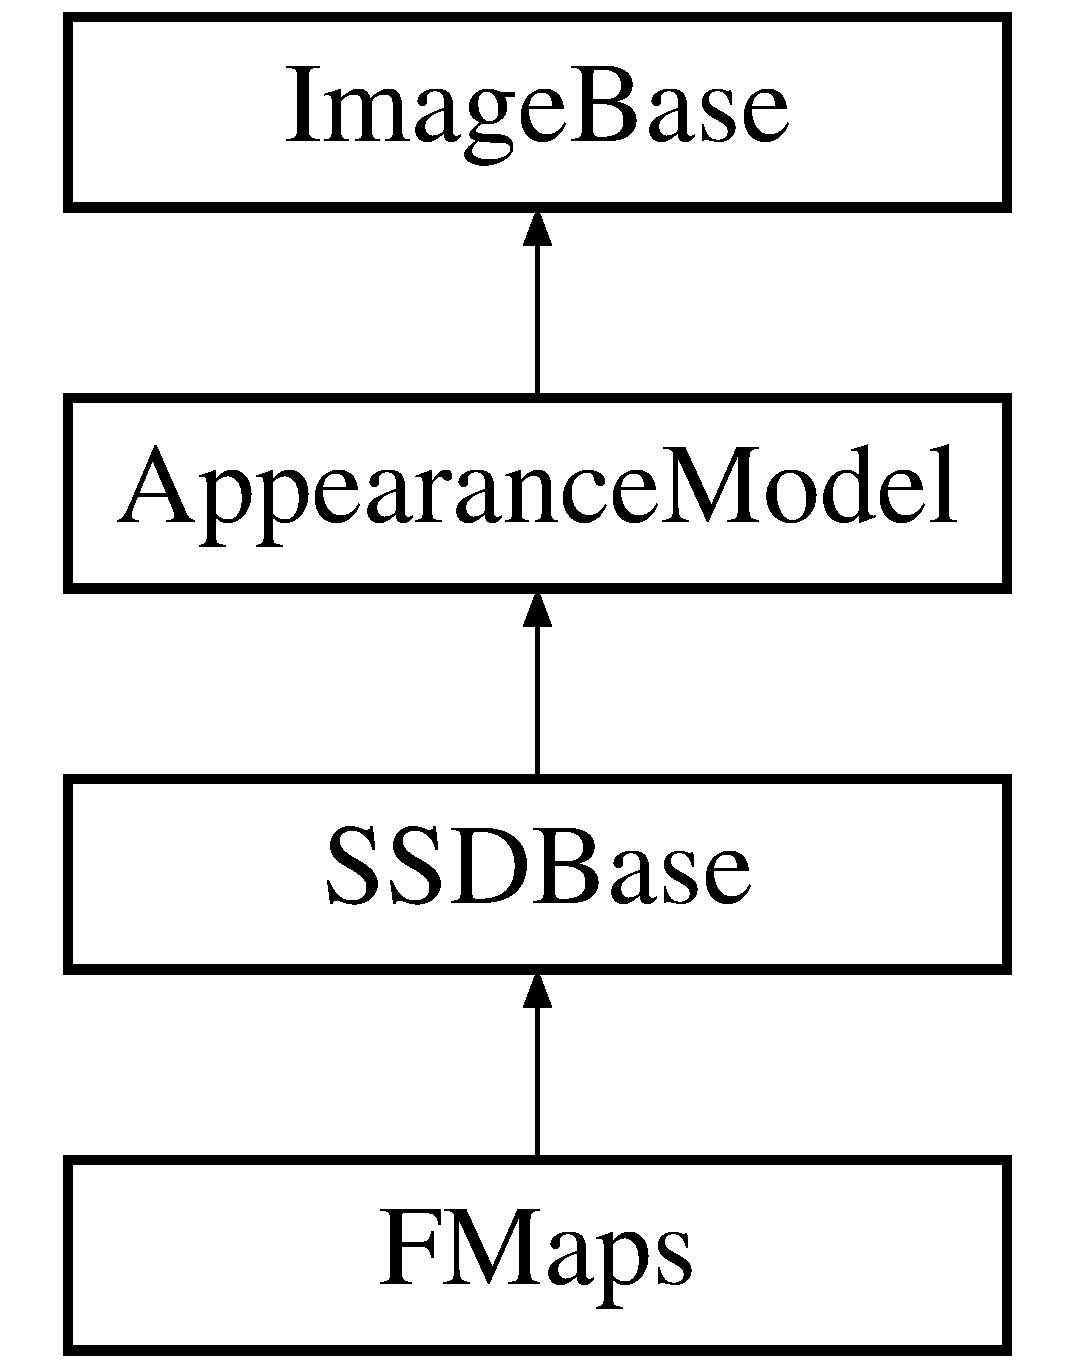
\includegraphics[height=4.000000cm]{classFMaps}
\end{center}
\end{figure}
\subsection*{Public Types}
\begin{DoxyCompactItemize}
\item 
\hypertarget{classFMaps_a10ab16ce3b844feafce5696d8b23a9db}{typedef \hyperlink{structFMapsParams}{F\-Maps\-Params} {\bfseries Param\-Type}}\label{classFMaps_a10ab16ce3b844feafce5696d8b23a9db}

\end{DoxyCompactItemize}
\subsection*{Public Member Functions}
\begin{DoxyCompactItemize}
\item 
\hypertarget{classFMaps_a90624adb93b1f985f1cb35b4b740cb8b}{{\bfseries F\-Maps} (const \hyperlink{structFMapsParams}{Param\-Type} $\ast$img\-\_\-params=nullptr)}\label{classFMaps_a90624adb93b1f985f1cb35b4b740cb8b}

\item 
\hypertarget{classFMaps_a48978383570fedc6c4a9231038c80207}{void \hyperlink{classFMaps_a48978383570fedc6c4a9231038c80207}{initialize\-Pix\-Vals} (const Matrix2\-Xd \&curr\-\_\-pts) override}\label{classFMaps_a48978383570fedc6c4a9231038c80207}

\begin{DoxyCompactList}\small\item\em initialization methods -\/ to be called once when the tracker is initialized \end{DoxyCompactList}\item 
\hypertarget{classFMaps_a3cf0e3ced00ada359e8e13702fbde5ed}{void {\bfseries update\-Pix\-Vals} (const Matrix2\-Xd \&curr\-\_\-pts) override}\label{classFMaps_a3cf0e3ced00ada359e8e13702fbde5ed}

\item 
\hypertarget{classFMaps_afc82e1a0e9812c81a418d3663953df77}{std\-::vector$<$ cv\-::\-Mat $>$ {\bfseries extract\-\_\-features} (cv\-::\-Mat img, char $\ast$layer\-\_\-name)}\label{classFMaps_afc82e1a0e9812c81a418d3663953df77}

\end{DoxyCompactItemize}
\subsection*{Public Attributes}
\begin{DoxyCompactItemize}
\item 
\hypertarget{classFMaps_ae1978e3808fcbc57ff4f50b80f7212a7}{\hyperlink{structFMapsParams}{Param\-Type} {\bfseries params}}\label{classFMaps_ae1978e3808fcbc57ff4f50b80f7212a7}

\item 
\hypertarget{classFMaps_a578407854d4b3eaeda8ee9ded324ca42}{Pix\-Val\-T {\bfseries init\-\_\-pix\-\_\-vals\-\_\-temp}}\label{classFMaps_a578407854d4b3eaeda8ee9ded324ca42}

\item 
\hypertarget{classFMaps_ad5dc00a5301ce072cae9988421fafc6c}{Pix\-Val\-T {\bfseries curr\-\_\-pix\-\_\-vals\-\_\-temp}}\label{classFMaps_ad5dc00a5301ce072cae9988421fafc6c}

\item 
\hypertarget{classFMaps_afe142767b6fa9cdf85f6fe4b3c879156}{Pix\-Val\-T {\bfseries temp\-\_\-fmaps}}\label{classFMaps_afe142767b6fa9cdf85f6fe4b3c879156}

\item 
\hypertarget{classFMaps_afe63a5bc25ac16f19bc3eaf376b0c043}{int {\bfseries n\-\_\-pix\-\_\-temp}}\label{classFMaps_afe63a5bc25ac16f19bc3eaf376b0c043}

\item 
\hypertarget{classFMaps_ac318d7b585ade6c1f3b2e508b744f752}{std\-::vector$<$ cv\-::\-Mat $>$ {\bfseries init\-\_\-fmaps}}\label{classFMaps_ac318d7b585ade6c1f3b2e508b744f752}

\item 
\hypertarget{classFMaps_adb736ba3698e5dcc55be8445b93f45c9}{std\-::vector$<$ cv\-::\-Mat $>$ {\bfseries curr\-\_\-fmaps}}\label{classFMaps_adb736ba3698e5dcc55be8445b93f45c9}

\item 
\hypertarget{classFMaps_a831136868b56c4c2ebb001d8eacfd2b5}{double \hyperlink{classFMaps_a831136868b56c4c2ebb001d8eacfd2b5}{init\-\_\-pix\-\_\-mean}}\label{classFMaps_a831136868b56c4c2ebb001d8eacfd2b5}

\begin{DoxyCompactList}\small\item\em mean, variance and standard deviation of the initial pixel values \end{DoxyCompactList}\item 
\hypertarget{classFMaps_ad424b30cdb035c4359b03963f53b419a}{double {\bfseries init\-\_\-pix\-\_\-var}}\label{classFMaps_ad424b30cdb035c4359b03963f53b419a}

\item 
\hypertarget{classFMaps_a4c470ad0517b859f1e08b237a8402a72}{double {\bfseries init\-\_\-pix\-\_\-std}}\label{classFMaps_a4c470ad0517b859f1e08b237a8402a72}

\item 
\hypertarget{classFMaps_adc41982dd716cd062e02074473944196}{double \hyperlink{classFMaps_adc41982dd716cd062e02074473944196}{curr\-\_\-pix\-\_\-mean}}\label{classFMaps_adc41982dd716cd062e02074473944196}

\begin{DoxyCompactList}\small\item\em mean, variance and standard deviation of the current pixel values \end{DoxyCompactList}\item 
\hypertarget{classFMaps_a6a6657178dce1776e0a46d93ff906e98}{double {\bfseries curr\-\_\-pix\-\_\-var}}\label{classFMaps_a6a6657178dce1776e0a46d93ff906e98}

\item 
\hypertarget{classFMaps_a80fc54b3c9604b6c5fd4a3f088961d7f}{double {\bfseries curr\-\_\-pix\-\_\-std}}\label{classFMaps_a80fc54b3c9604b6c5fd4a3f088961d7f}

\item 
\hypertarget{classFMaps_a84ebd30954b0e7a001c3eb5bd2b980aa}{int {\bfseries nfmaps}}\label{classFMaps_a84ebd30954b0e7a001c3eb5bd2b980aa}

\item 
\hypertarget{classFMaps_a4515435f6681cbf800cc6fc347dde8f0}{char $\ast$ {\bfseries layer\-\_\-name}}\label{classFMaps_a4515435f6681cbf800cc6fc347dde8f0}

\item 
\hypertarget{classFMaps_afb2805b98c7e5f7d6d1d2887fca7d0b3}{int {\bfseries vis}}\label{classFMaps_afb2805b98c7e5f7d6d1d2887fca7d0b3}

\item 
\hypertarget{classFMaps_adea04d75ab3dd06d4c3babed473805c3}{int {\bfseries e\-\_\-zncc}}\label{classFMaps_adea04d75ab3dd06d4c3babed473805c3}

\end{DoxyCompactItemize}
\subsection*{Static Public Attributes}
\begin{DoxyCompactItemize}
\item 
\hypertarget{classFMaps_aaab0422bb392800bea1572e36fd63313}{static \hyperlink{structFMapsParams}{Param\-Type} {\bfseries static\-\_\-params}}\label{classFMaps_aaab0422bb392800bea1572e36fd63313}

\end{DoxyCompactItemize}
\subsection*{Additional Inherited Members}


The documentation for this class was generated from the following file\-:\begin{DoxyCompactItemize}
\item 
A\-M/include/mtf/\-A\-M/F\-Maps.\-h\end{DoxyCompactItemize}

\hypertarget{structFMapsParams}{\section{F\-Maps\-Params Struct Reference}
\label{structFMapsParams}\index{F\-Maps\-Params@{F\-Maps\-Params}}
}
Inheritance diagram for F\-Maps\-Params\-:\begin{figure}[H]
\begin{center}
\leavevmode
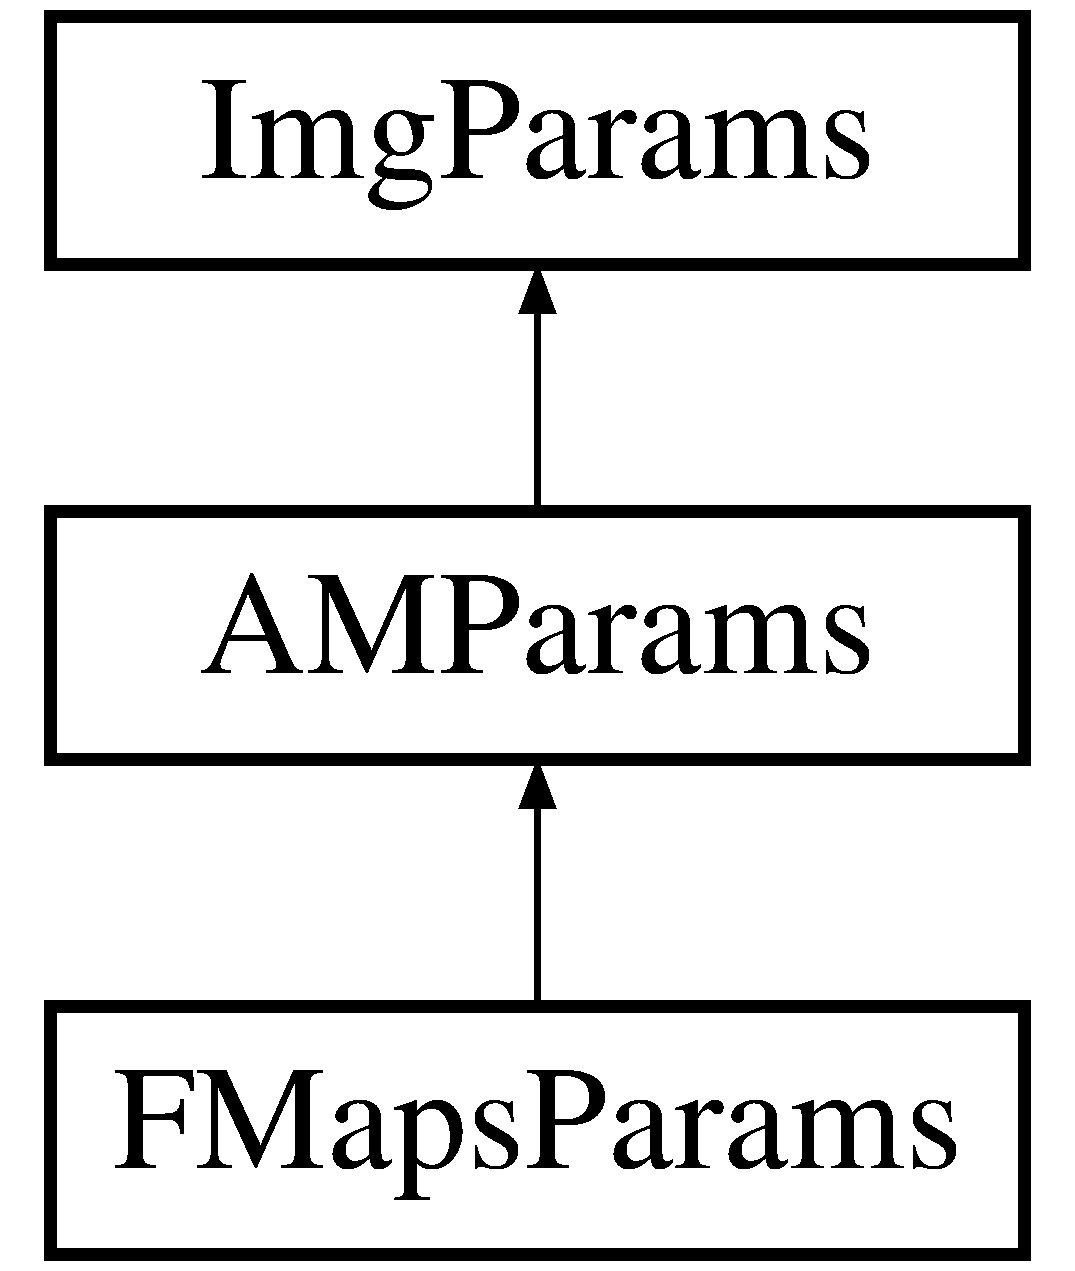
\includegraphics[height=3.000000cm]{structFMapsParams}
\end{center}
\end{figure}
\subsection*{Public Member Functions}
\begin{DoxyCompactItemize}
\item 
\hypertarget{structFMapsParams_a0b84c8b27120148ff0525d777f2c5773}{\hyperlink{structFMapsParams_a0b84c8b27120148ff0525d777f2c5773}{F\-Maps\-Params} (const \hyperlink{structAMParams}{A\-M\-Params} $\ast$am\-\_\-params, int \-\_\-n\-\_\-fmaps, char $\ast$\-\_\-layer\-\_\-name, int \-\_\-vis, int \-\_\-zncc, char $\ast$\-\_\-model\-\_\-f\-\_\-name, char $\ast$\-\_\-mean\-\_\-f\-\_\-name, char $\ast$\-\_\-params\-\_\-f\-\_\-name)}\label{structFMapsParams_a0b84c8b27120148ff0525d777f2c5773}

\begin{DoxyCompactList}\small\item\em value constructor \end{DoxyCompactList}\item 
\hypertarget{structFMapsParams_a28043c4e323a356f7865366c532b0677}{\hyperlink{structFMapsParams_a28043c4e323a356f7865366c532b0677}{F\-Maps\-Params} (const \hyperlink{structFMapsParams}{F\-Maps\-Params} $\ast$params=nullptr)}\label{structFMapsParams_a28043c4e323a356f7865366c532b0677}

\begin{DoxyCompactList}\small\item\em default/copy constructor \end{DoxyCompactList}\end{DoxyCompactItemize}
\subsection*{Public Attributes}
\begin{DoxyCompactItemize}
\item 
\hypertarget{structFMapsParams_a605b83b6860dd8decc72d8aed3c07650}{int {\bfseries nfmaps}}\label{structFMapsParams_a605b83b6860dd8decc72d8aed3c07650}

\item 
\hypertarget{structFMapsParams_abc7892296a5aaee60c7ff7bbea76ad4c}{char $\ast$ {\bfseries layer\-\_\-name}}\label{structFMapsParams_abc7892296a5aaee60c7ff7bbea76ad4c}

\item 
\hypertarget{structFMapsParams_abd2e905d6f4f8287d9c8b6dae91b7e58}{int {\bfseries vis}}\label{structFMapsParams_abd2e905d6f4f8287d9c8b6dae91b7e58}

\item 
\hypertarget{structFMapsParams_a716dda3953dac62610821998196f7e92}{int {\bfseries e\-\_\-zncc}}\label{structFMapsParams_a716dda3953dac62610821998196f7e92}

\item 
\hypertarget{structFMapsParams_a335882b284535adf536cef6cc990c859}{char $\ast$ {\bfseries model\-\_\-file\-\_\-name}}\label{structFMapsParams_a335882b284535adf536cef6cc990c859}

\item 
\hypertarget{structFMapsParams_a03825ed5283c2bec2078e97cafecdeb9}{char $\ast$ {\bfseries mean\-\_\-file\-\_\-name}}\label{structFMapsParams_a03825ed5283c2bec2078e97cafecdeb9}

\item 
\hypertarget{structFMapsParams_a31fa30b5fd632b648d292bfd829de57d}{char $\ast$ {\bfseries params\-\_\-file\-\_\-name}}\label{structFMapsParams_a31fa30b5fd632b648d292bfd829de57d}

\end{DoxyCompactItemize}


The documentation for this struct was generated from the following file\-:\begin{DoxyCompactItemize}
\item 
A\-M/include/mtf/\-A\-M/F\-Maps.\-h\end{DoxyCompactItemize}

\hypertarget{classutils_1_1FunctonNotImplemented}{\section{utils\-:\-:Functon\-Not\-Implemented Class Reference}
\label{classutils_1_1FunctonNotImplemented}\index{utils\-::\-Functon\-Not\-Implemented@{utils\-::\-Functon\-Not\-Implemented}}
}
Inheritance diagram for utils\-:\-:Functon\-Not\-Implemented\-:\begin{figure}[H]
\begin{center}
\leavevmode
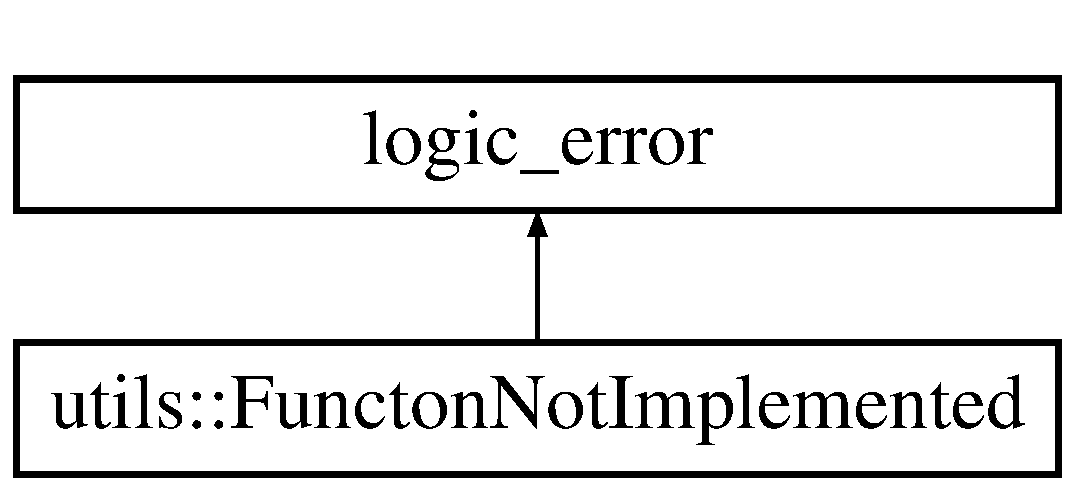
\includegraphics[height=2.000000cm]{classutils_1_1FunctonNotImplemented}
\end{center}
\end{figure}
\subsection*{Public Member Functions}
\begin{DoxyCompactItemize}
\item 
\hypertarget{classutils_1_1FunctonNotImplemented_a59e04ef4b1a20a63b73df7ac9857e6e7}{{\bfseries Functon\-Not\-Implemented} (const char $\ast$error=\char`\"{}Function has not been implemented yet\char`\"{})}\label{classutils_1_1FunctonNotImplemented_a59e04ef4b1a20a63b73df7ac9857e6e7}

\item 
\hypertarget{classutils_1_1FunctonNotImplemented_a2dd8da4f1b1bf70aece415f1d4854693}{{\bfseries Functon\-Not\-Implemented} (const std\-::string error=\char`\"{}Function has not been implemented yet\char`\"{})}\label{classutils_1_1FunctonNotImplemented_a2dd8da4f1b1bf70aece415f1d4854693}

\end{DoxyCompactItemize}


The documentation for this class was generated from the following file\-:\begin{DoxyCompactItemize}
\item 
Utilities/include/mtf/\-Utilities/excp\-Utils.\-h\end{DoxyCompactItemize}

\hypertarget{classGB}{\section{G\-B Class Reference}
\label{classGB}\index{G\-B@{G\-B}}
}
Inheritance diagram for G\-B\-:\begin{figure}[H]
\begin{center}
\leavevmode
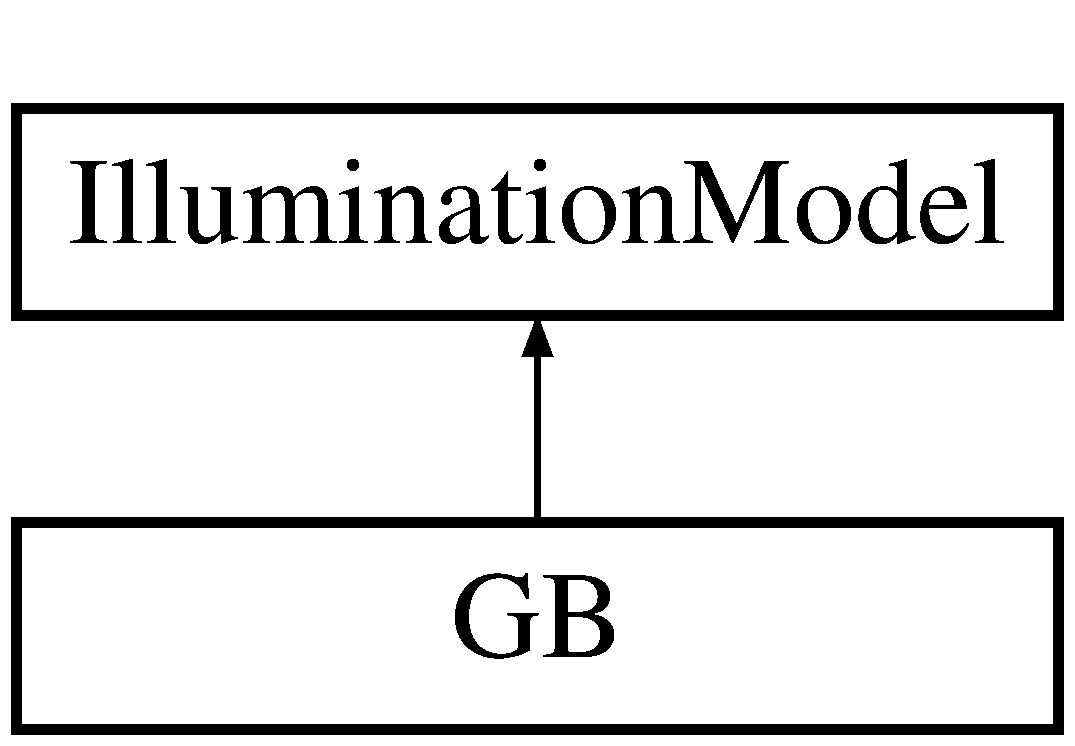
\includegraphics[height=2.000000cm]{classGB}
\end{center}
\end{figure}
\subsection*{Public Types}
\begin{DoxyCompactItemize}
\item 
\hypertarget{classGB_a0772c7b02b95046a221df78fb3b9b77f}{typedef \hyperlink{structGBParams}{G\-B\-Params} {\bfseries Param\-Type}}\label{classGB_a0772c7b02b95046a221df78fb3b9b77f}

\end{DoxyCompactItemize}
\subsection*{Public Member Functions}
\begin{DoxyCompactItemize}
\item 
\hypertarget{classGB_a7692207db0c1e4dc3c89af8b9eb111bf}{{\bfseries G\-B} (const \hyperlink{structGBParams}{Param\-Type} $\ast$\-\_\-gb\-\_\-params=nullptr)}\label{classGB_a7692207db0c1e4dc3c89af8b9eb111bf}

\item 
\hypertarget{classGB_a775656c003d6b3c9a8ad9879ab7c7ca9}{void {\bfseries initialize} (double $\ast$p) override}\label{classGB_a775656c003d6b3c9a8ad9879ab7c7ca9}

\item 
\hypertarget{classGB_ab0cfbf84d291d17b93be0e6d483a09aa}{int {\bfseries get\-State\-Size} () const override}\label{classGB_ab0cfbf84d291d17b93be0e6d483a09aa}

\item 
\hypertarget{classGB_a40647dc4b03eec10d285fe962af24e6e}{void {\bfseries apply} (double $\ast$g, const double $\ast$I, const double $\ast$p) override}\label{classGB_a40647dc4b03eec10d285fe962af24e6e}

\item 
\hypertarget{classGB_abc254f11815b01d3ac6fcc49f4800139}{void {\bfseries invert} (double $\ast$inv\-\_\-p, const double $\ast$p) override}\label{classGB_abc254f11815b01d3ac6fcc49f4800139}

\item 
\hypertarget{classGB_a0c67cd2ac56b1e9ee6abfa925f84eec6}{void {\bfseries update} (double $\ast$new\-\_\-p, const double $\ast$old\-\_\-p, const double $\ast$dp) override}\label{classGB_a0c67cd2ac56b1e9ee6abfa925f84eec6}

\item 
\hypertarget{classGB_a5f044dfbaa8519503bfb19517e835b25}{void {\bfseries cmpt\-Param\-Jacobian} (double $\ast$df\-\_\-dp, const double $\ast$df\-\_\-dg, const double $\ast$I, const double $\ast$p) override}\label{classGB_a5f044dfbaa8519503bfb19517e835b25}

\item 
\hypertarget{classGB_a011223e61c83eec2809b2b898b6de52d}{void {\bfseries cmpt\-Param\-Hessian} (double $\ast$d2f\-\_\-dp2, const double $\ast$d2f\-\_\-dg2, const double $\ast$df\-\_\-dg, const double $\ast$I, const double $\ast$p) override}\label{classGB_a011223e61c83eec2809b2b898b6de52d}

\item 
\hypertarget{classGB_a66cb01d0cd132d8ef8d43c2d866142c9}{void {\bfseries cmpt\-Pix\-Jacobian} (double $\ast$df\-\_\-d\-I, const double $\ast$df\-\_\-dg, const double $\ast$I, const double $\ast$p) override}\label{classGB_a66cb01d0cd132d8ef8d43c2d866142c9}

\item 
\hypertarget{classGB_ad01931c3cfa3f53499256ad3bd627860}{void {\bfseries cmpt\-Pix\-Hessian} (double $\ast$d2f\-\_\-d\-I2, const double $\ast$d2f\-\_\-dg2, const double $\ast$df\-\_\-dg, const double $\ast$I, const double $\ast$p) override}\label{classGB_ad01931c3cfa3f53499256ad3bd627860}

\item 
\hypertarget{classGB_a8e3a6fbe468066d6d28afc5e8106182a}{void {\bfseries cmpt\-Cross\-Hessian} (double $\ast$d2f\-\_\-dp\-\_\-d\-I, const double $\ast$d2f\-\_\-dg2, const double $\ast$df\-\_\-dg, const double $\ast$I, const double $\ast$p) override}\label{classGB_a8e3a6fbe468066d6d28afc5e8106182a}

\item 
\hypertarget{classGB_ac0db45fd0f4075ede025b904168e4d6e}{Pix\-Hess\-Type {\bfseries get\-Pix\-Hess\-Type} () override}\label{classGB_ac0db45fd0f4075ede025b904168e4d6e}

\end{DoxyCompactItemize}
\subsection*{Protected Attributes}
\begin{DoxyCompactItemize}
\item 
\hypertarget{classGB_a9998ce554bb94602706dbdf6c4618bde}{\hyperlink{structGBParams}{Param\-Type} {\bfseries params}}\label{classGB_a9998ce554bb94602706dbdf6c4618bde}

\end{DoxyCompactItemize}
\subsection*{Additional Inherited Members}


The documentation for this class was generated from the following file\-:\begin{DoxyCompactItemize}
\item 
A\-M/include/mtf/\-A\-M/G\-B.\-h\end{DoxyCompactItemize}

\hypertarget{structGBParams}{\section{G\-B\-Params Struct Reference}
\label{structGBParams}\index{G\-B\-Params@{G\-B\-Params}}
}
Inheritance diagram for G\-B\-Params\-:\begin{figure}[H]
\begin{center}
\leavevmode
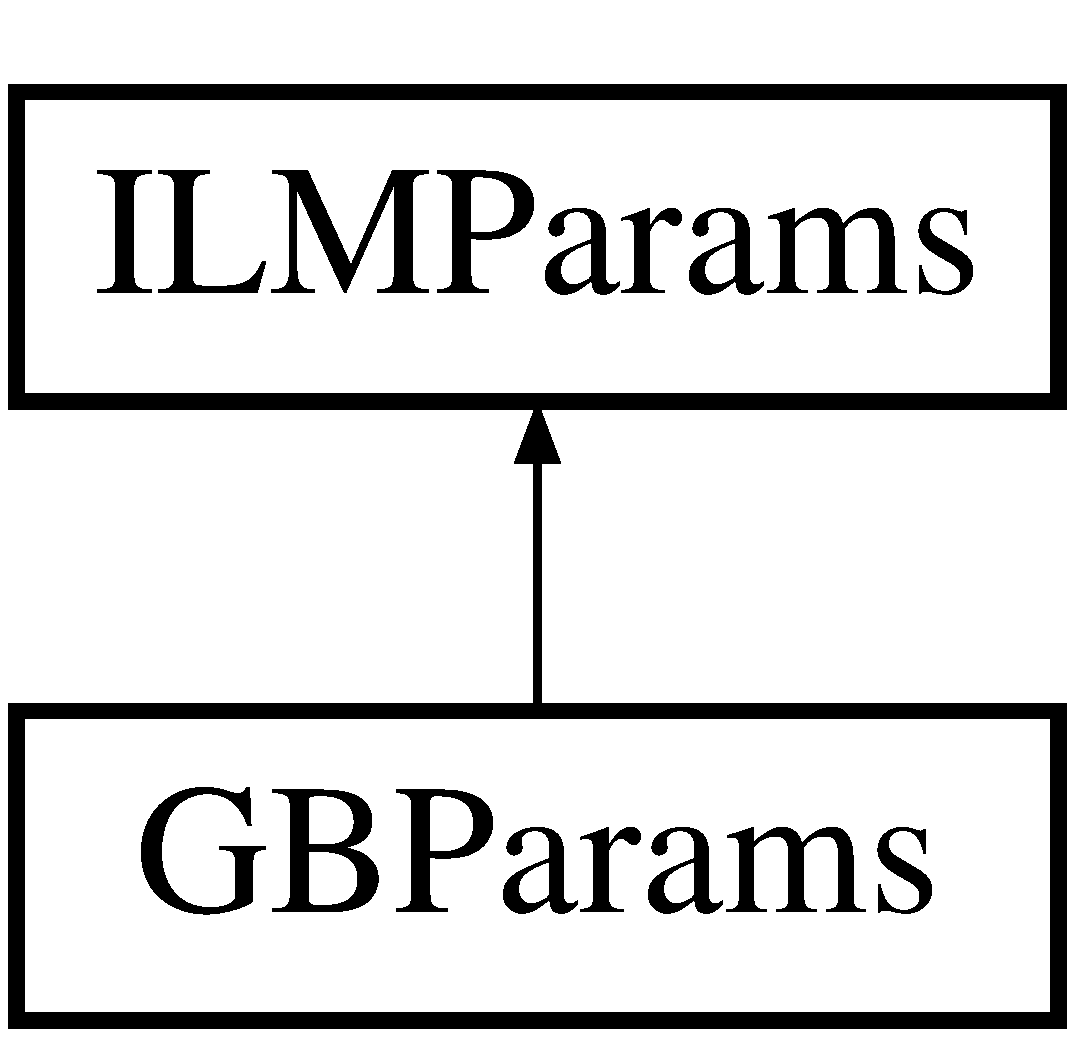
\includegraphics[height=2.000000cm]{structGBParams}
\end{center}
\end{figure}
\subsection*{Public Member Functions}
\begin{DoxyCompactItemize}
\item 
\hypertarget{structGBParams_a3e0b0413313c47a11314d99eea563306}{\hyperlink{structGBParams_a3e0b0413313c47a11314d99eea563306}{G\-B\-Params} (\hyperlink{structILMParams}{I\-L\-M\-Params} $\ast$ilm\-\_\-params, bool \-\_\-additive\-\_\-update)}\label{structGBParams_a3e0b0413313c47a11314d99eea563306}

\begin{DoxyCompactList}\small\item\em value constructor \end{DoxyCompactList}\item 
\hypertarget{structGBParams_a5529d27c4a62dcade263a353efbd7d50}{\hyperlink{structGBParams_a5529d27c4a62dcade263a353efbd7d50}{G\-B\-Params} (const \hyperlink{structGBParams}{G\-B\-Params} $\ast$params=nullptr)}\label{structGBParams_a5529d27c4a62dcade263a353efbd7d50}

\begin{DoxyCompactList}\small\item\em default/copy constructor \end{DoxyCompactList}\end{DoxyCompactItemize}
\subsection*{Public Attributes}
\begin{DoxyCompactItemize}
\item 
\hypertarget{structGBParams_a90fee7300b2bad14230e31cd1ed253a8}{bool {\bfseries additive\-\_\-update}}\label{structGBParams_a90fee7300b2bad14230e31cd1ed253a8}

\end{DoxyCompactItemize}


The documentation for this struct was generated from the following file\-:\begin{DoxyCompactItemize}
\item 
A\-M/include/mtf/\-A\-M/G\-B.\-h\end{DoxyCompactItemize}

\hypertarget{classgnn_1_1GNN}{\section{gnn\-:\-:G\-N\-N$<$ A\-M $>$ Class Template Reference}
\label{classgnn_1_1GNN}\index{gnn\-::\-G\-N\-N$<$ A\-M $>$@{gnn\-::\-G\-N\-N$<$ A\-M $>$}}
}
Inheritance diagram for gnn\-:\-:G\-N\-N$<$ A\-M $>$\-:\begin{figure}[H]
\begin{center}
\leavevmode
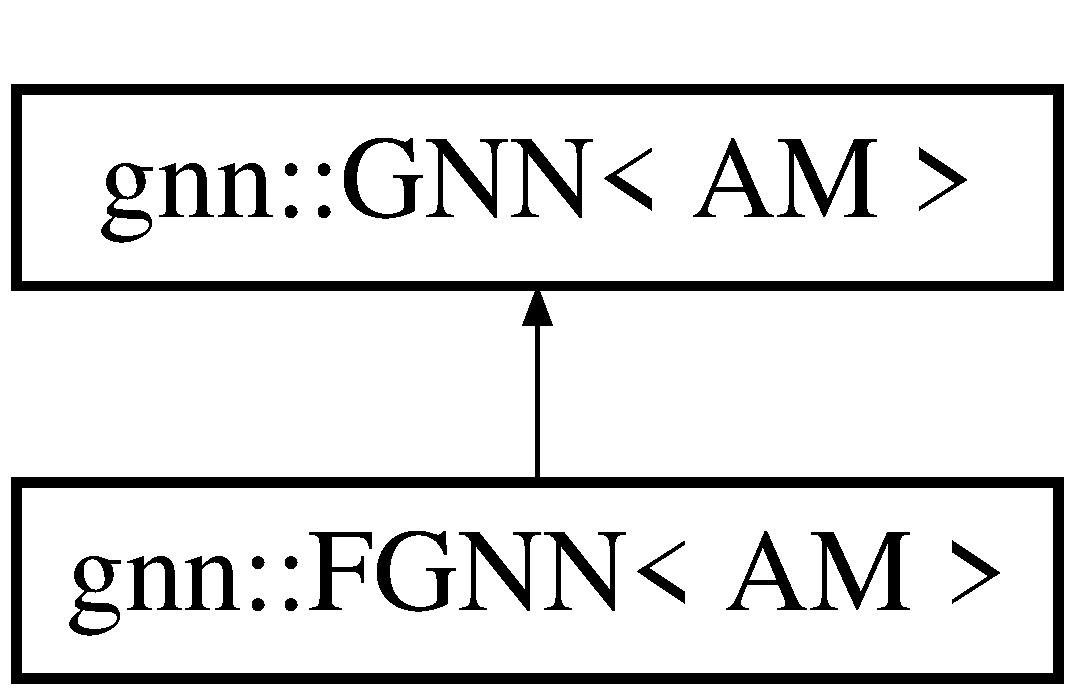
\includegraphics[height=2.000000cm]{classgnn_1_1GNN}
\end{center}
\end{figure}
\subsection*{Public Types}
\begin{DoxyCompactItemize}
\item 
\hypertarget{classgnn_1_1GNN_a45509461044fc7a8c2c9e8f1541b354d}{typedef \hyperlink{structgnn_1_1GNNParams}{G\-N\-N\-Params} {\bfseries Param\-Type}}\label{classgnn_1_1GNN_a45509461044fc7a8c2c9e8f1541b354d}

\end{DoxyCompactItemize}
\subsection*{Public Member Functions}
\begin{DoxyCompactItemize}
\item 
\hypertarget{classgnn_1_1GNN_a3ef3c7eca7fa61304ded6b74e736b9c3}{{\bfseries G\-N\-N} (const A\-M $\ast$\-\_\-dist\-\_\-func, int \-\_\-n\-\_\-samples, int \-\_\-n\-\_\-dims, bool \-\_\-is\-\_\-symmetrical=true, const \hyperlink{structgnn_1_1GNNParams}{Param\-Type} $\ast$gnn\-\_\-params=nullptr)}\label{classgnn_1_1GNN_a3ef3c7eca7fa61304ded6b74e736b9c3}

\item 
\hypertarget{classgnn_1_1GNN_a041899e3872c67753c7f6635691ef45d}{void {\bfseries compute\-Distances} (const double $\ast$dataset)}\label{classgnn_1_1GNN_a041899e3872c67753c7f6635691ef45d}

\item 
\hypertarget{classgnn_1_1GNN_a895f34aeb9d6c1f2a40e23b2dba36a65}{void {\bfseries build\-Graph} (const double $\ast$dataset)}\label{classgnn_1_1GNN_a895f34aeb9d6c1f2a40e23b2dba36a65}

\item 
\hypertarget{classgnn_1_1GNN_a7b56ab242b2b0aaaf4e1377521d9fb20}{void {\bfseries search\-Graph} (const double $\ast$query, const double $\ast$dataset, int $\ast$nn\-\_\-ids, double $\ast$nn\-\_\-dists, int K=1)}\label{classgnn_1_1GNN_a7b56ab242b2b0aaaf4e1377521d9fb20}

\item 
\hypertarget{classgnn_1_1GNN_aef78402a962fca21ff078de246714e6c}{void {\bfseries save\-Graph} (const char $\ast$file\-\_\-name)}\label{classgnn_1_1GNN_aef78402a962fca21ff078de246714e6c}

\item 
\hypertarget{classgnn_1_1GNN_a460a8d8c984558c55f28c4d7b54c5e18}{void {\bfseries load\-Graph} (const char $\ast$file\-\_\-name)}\label{classgnn_1_1GNN_a460a8d8c984558c55f28c4d7b54c5e18}

\item 
\hypertarget{classgnn_1_1GNN_a8c8cf493de68e3abad95d8c5413e5375}{void {\bfseries build\-Graph} (const double $\ast$X, int k)}\label{classgnn_1_1GNN_a8c8cf493de68e3abad95d8c5413e5375}

\item 
\hypertarget{classgnn_1_1GNN_aef87dcda4d56d55e17712e204ead65c1}{int {\bfseries search\-Graph} (const double $\ast$Xq, const double $\ast$X, int N\-Ns, int K)}\label{classgnn_1_1GNN_aef87dcda4d56d55e17712e204ead65c1}

\end{DoxyCompactItemize}
\subsection*{Protected Member Functions}
\begin{DoxyCompactItemize}
\item 
\hypertarget{classgnn_1_1GNN_ae6e5a1a1622c6499805be134fd96ca36}{int {\bfseries get\-Rand\-Num} (int lb, int ub)}\label{classgnn_1_1GNN_ae6e5a1a1622c6499805be134fd96ca36}

\item 
\hypertarget{classgnn_1_1GNN_a5020e3d998563b2279b0a4d125dad109}{{\footnotesize template$<$typename Scalar\-T $>$ }\\void {\bfseries swap} (Scalar\-T $\ast$i, Scalar\-T $\ast$j)}\label{classgnn_1_1GNN_a5020e3d998563b2279b0a4d125dad109}

\item 
\hypertarget{classgnn_1_1GNN_a8a4b8d1a5201f6c15b46d33a953889bc}{void {\bfseries knn\-Search2} (const double $\ast$Q, \hyperlink{structgnn_1_1IndxDist}{Indx\-Dist} $\ast$dists, const double $\ast$X, int rows, int cols, int k)}\label{classgnn_1_1GNN_a8a4b8d1a5201f6c15b46d33a953889bc}

\item 
\hypertarget{classgnn_1_1GNN_aeb77b996e512dd021a922d3f8aa2ef75}{void {\bfseries knn\-Search11} (const double $\ast$Q, \hyperlink{structgnn_1_1IndxDist}{Indx\-Dist} $\ast$dists, const double $\ast$X, int rows, int cols, int k, int $\ast$X\-\_\-inds)}\label{classgnn_1_1GNN_aeb77b996e512dd021a922d3f8aa2ef75}

\item 
\hypertarget{classgnn_1_1GNN_ad3a945133912195829a28db482d289ca}{int {\bfseries min} (int a, int b)}\label{classgnn_1_1GNN_ad3a945133912195829a28db482d289ca}

\item 
\hypertarget{classgnn_1_1GNN_a9d769573a9aef4d4b35047989c82de89}{void {\bfseries pick\-K\-N\-Ns} (\hyperlink{structgnn_1_1IndxDist}{Indx\-Dist} $\ast$vis\-\_\-nodes, int visited, \hyperlink{structgnn_1_1IndxDist}{Indx\-Dist} $\ast$$\ast$gnn\-\_\-dists, int K, int $\ast$gnns\-\_\-cap)}\label{classgnn_1_1GNN_a9d769573a9aef4d4b35047989c82de89}

\item 
\hypertarget{classgnn_1_1GNN_a2d8add065ffda33d9c4b56c431bbd67f}{void {\bfseries add\-Node} (\hyperlink{structgnn_1_1Node}{Node} $\ast$node\-\_\-i, int nn)}\label{classgnn_1_1GNN_a2d8add065ffda33d9c4b56c431bbd67f}

\end{DoxyCompactItemize}
\subsection*{Protected Attributes}
\begin{DoxyCompactItemize}
\item 
\hypertarget{classgnn_1_1GNN_a3ac4ebdff631df1852fbeebef513230b}{const A\-M $\ast$ {\bfseries dist\-\_\-func}}\label{classgnn_1_1GNN_a3ac4ebdff631df1852fbeebef513230b}

\item 
\hypertarget{classgnn_1_1GNN_aab908567c880074067e9ca6e332ed66f}{const int {\bfseries n\-\_\-samples}}\label{classgnn_1_1GNN_aab908567c880074067e9ca6e332ed66f}

\item 
\hypertarget{classgnn_1_1GNN_a70eab0aebf2978f956da3b9473388219}{const int {\bfseries n\-\_\-dims}}\label{classgnn_1_1GNN_a70eab0aebf2978f956da3b9473388219}

\item 
\hypertarget{classgnn_1_1GNN_a06f37f0a5fd5133a600c22bd4ae4d95b}{const bool {\bfseries is\-\_\-symmetrical}}\label{classgnn_1_1GNN_a06f37f0a5fd5133a600c22bd4ae4d95b}

\item 
\hypertarget{classgnn_1_1GNN_a49104d6ec9519fa8c19307639c8571ba}{\hyperlink{structgnn_1_1GNNParams}{Param\-Type} {\bfseries params}}\label{classgnn_1_1GNN_a49104d6ec9519fa8c19307639c8571ba}

\item 
\hypertarget{classgnn_1_1GNN_a5ed6bcf9456fde5882e230f20e71b6b4}{\hyperlink{structgnn_1_1Node}{Node} $\ast$ {\bfseries nodes}}\label{classgnn_1_1GNN_a5ed6bcf9456fde5882e230f20e71b6b4}

\item 
\hypertarget{classgnn_1_1GNN_a73c75358d06d65299f143e117d3e3c13}{Matrix\-Xd {\bfseries dataset\-\_\-distances}}\label{classgnn_1_1GNN_a73c75358d06d65299f143e117d3e3c13}

\item 
\hypertarget{classgnn_1_1GNN_a0b418512ff0aa7b8ce2f8ca0cc3dcbf9}{int {\bfseries start\-\_\-node\-\_\-idx}}\label{classgnn_1_1GNN_a0b418512ff0aa7b8ce2f8ca0cc3dcbf9}

\item 
\hypertarget{classgnn_1_1GNN_ac07236c6c6325311cbd861735418272d}{bool {\bfseries dist\-\_\-computed}}\label{classgnn_1_1GNN_ac07236c6c6325311cbd861735418272d}

\end{DoxyCompactItemize}


The documentation for this class was generated from the following file\-:\begin{DoxyCompactItemize}
\item 
S\-M/include/mtf/\-S\-M/G\-N\-N.\-h\end{DoxyCompactItemize}

\hypertarget{structgnn_1_1GNNParams}{\section{gnn\-:\-:G\-N\-N\-Params Struct Reference}
\label{structgnn_1_1GNNParams}\index{gnn\-::\-G\-N\-N\-Params@{gnn\-::\-G\-N\-N\-Params}}
}
\subsection*{Public Member Functions}
\begin{DoxyCompactItemize}
\item 
\hypertarget{structgnn_1_1GNNParams_a74afc84fec78df4ce57a44ef0145b1ac}{{\bfseries G\-N\-N\-Params} (int \-\_\-dgree, int \-\_\-max\-\_\-steps, int \-\_\-cmpt\-\_\-dist\-\_\-thresh, bool \-\_\-verbose)}\label{structgnn_1_1GNNParams_a74afc84fec78df4ce57a44ef0145b1ac}

\item 
\hypertarget{structgnn_1_1GNNParams_adcb6594bc3f8fa667738ad8d42bca387}{{\bfseries G\-N\-N\-Params} (const \hyperlink{structgnn_1_1GNNParams}{G\-N\-N\-Params} $\ast$params=nullptr)}\label{structgnn_1_1GNNParams_adcb6594bc3f8fa667738ad8d42bca387}

\item 
\hypertarget{structgnn_1_1GNNParams_a74afc84fec78df4ce57a44ef0145b1ac}{{\bfseries G\-N\-N\-Params} (int \-\_\-dgree, int \-\_\-max\-\_\-steps, int \-\_\-cmpt\-\_\-dist\-\_\-thresh, bool \-\_\-verbose)}\label{structgnn_1_1GNNParams_a74afc84fec78df4ce57a44ef0145b1ac}

\item 
\hypertarget{structgnn_1_1GNNParams_adcb6594bc3f8fa667738ad8d42bca387}{{\bfseries G\-N\-N\-Params} (const \hyperlink{structgnn_1_1GNNParams}{G\-N\-N\-Params} $\ast$params=nullptr)}\label{structgnn_1_1GNNParams_adcb6594bc3f8fa667738ad8d42bca387}

\end{DoxyCompactItemize}
\subsection*{Public Attributes}
\begin{DoxyCompactItemize}
\item 
\hypertarget{structgnn_1_1GNNParams_ae23925798a97275ddf231e8f159e564e}{int {\bfseries degree}}\label{structgnn_1_1GNNParams_ae23925798a97275ddf231e8f159e564e}

\item 
\hypertarget{structgnn_1_1GNNParams_adeb934339aaaa3338573717b5310f8bf}{int {\bfseries max\-\_\-steps}}\label{structgnn_1_1GNNParams_adeb934339aaaa3338573717b5310f8bf}

\item 
\hypertarget{structgnn_1_1GNNParams_a65ce004484c30e95c3a0882b3e947c40}{int {\bfseries cmpt\-\_\-dist\-\_\-thresh}}\label{structgnn_1_1GNNParams_a65ce004484c30e95c3a0882b3e947c40}

\item 
\hypertarget{structgnn_1_1GNNParams_a86829c23acb6d7b6a95c8c568116f1a4}{bool {\bfseries verbose}}\label{structgnn_1_1GNNParams_a86829c23acb6d7b6a95c8c568116f1a4}

\end{DoxyCompactItemize}


The documentation for this struct was generated from the following files\-:\begin{DoxyCompactItemize}
\item 
S\-M/include/mtf/\-S\-M/G\-N\-N.\-h\item 
S\-M/include/mtf/\-S\-M/G\-N\-N\-Params.\-h\end{DoxyCompactItemize}

\hypertarget{classGridBase}{\section{Grid\-Base Class Reference}
\label{classGridBase}\index{Grid\-Base@{Grid\-Base}}
}
Inheritance diagram for Grid\-Base\-:\begin{figure}[H]
\begin{center}
\leavevmode
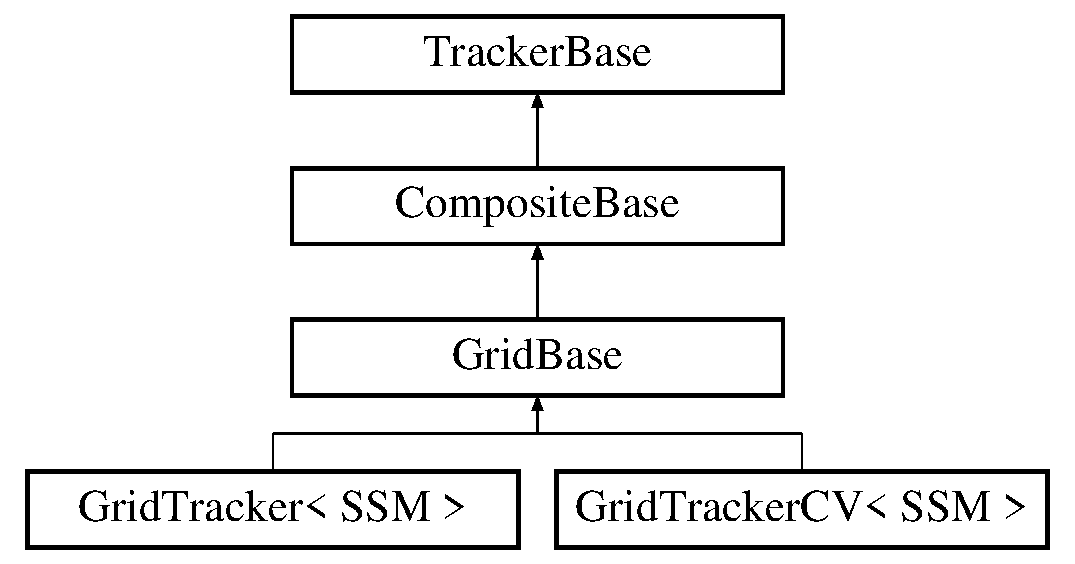
\includegraphics[height=4.000000cm]{classGridBase}
\end{center}
\end{figure}
\subsection*{Public Member Functions}
\begin{DoxyCompactItemize}
\item 
\hypertarget{classGridBase_af165e20266a2dded0102bdeefae83c24}{{\bfseries Grid\-Base} (const vector$<$ Tracker\-Base $\ast$ $>$ \-\_\-trackers)}\label{classGridBase_af165e20266a2dded0102bdeefae83c24}

\item 
\hypertarget{classGridBase_a7f30bfa6984c94af44ed156e4a294c3f}{virtual const uchar $\ast$ {\bfseries get\-Pix\-Mask} ()=0}\label{classGridBase_a7f30bfa6984c94af44ed156e4a294c3f}

\item 
\hypertarget{classGridBase_a6d3d5661688161ef6f5e0acc66572af2}{virtual int {\bfseries get\-Res\-X} ()=0}\label{classGridBase_a6d3d5661688161ef6f5e0acc66572af2}

\item 
\hypertarget{classGridBase_a3a72f50590abc5c17f4eeef62b664e23}{virtual int {\bfseries get\-Res\-Y} ()=0}\label{classGridBase_a3a72f50590abc5c17f4eeef62b664e23}

\end{DoxyCompactItemize}
\subsection*{Additional Inherited Members}


The documentation for this class was generated from the following file\-:\begin{DoxyCompactItemize}
\item 
S\-M/include/mtf/\-S\-M/Grid\-Base.\-h\end{DoxyCompactItemize}

\hypertarget{structgridLine}{\section{grid\-Line Struct Reference}
\label{structgridLine}\index{grid\-Line@{grid\-Line}}
}
\subsection*{Public Member Functions}
\begin{DoxyCompactItemize}
\item 
\hypertarget{structgridLine_a7a18615917f0eac76afab32739f94850}{void {\bfseries init} (int no\-\_\-of\-\_\-pts, int type)}\label{structgridLine_a7a18615917f0eac76afab32739f94850}

\item 
\hypertarget{structgridLine_a7272c7473adde2902ff86db92c5b550e}{void {\bfseries assign\-Addrs} (\hyperlink{structgridPoint}{grid\-Point} $\ast$start\-\_\-addr=nullptr, int offset\-\_\-diff=1)}\label{structgridLine_a7272c7473adde2902ff86db92c5b550e}

\item 
\hypertarget{structgridLine_a3b59b87a28f59ed0c0670e704d53ad90}{void {\bfseries update\-Params} ()}\label{structgridLine_a3b59b87a28f59ed0c0670e704d53ad90}

\end{DoxyCompactItemize}
\subsection*{Public Attributes}
\begin{DoxyCompactItemize}
\item 
\hypertarget{structgridLine_ac8dc3cd39f72773e274f39c0e5e97c06}{int {\bfseries no\-\_\-of\-\_\-pts}}\label{structgridLine_ac8dc3cd39f72773e274f39c0e5e97c06}

\item 
\hypertarget{structgridLine_ac171008c86f36f23688162b69668b58b}{\hyperlink{structlineParams}{line\-Params} $\ast$ {\bfseries params}}\label{structgridLine_ac171008c86f36f23688162b69668b58b}

\item 
\hypertarget{structgridLine_ab889d21c3255f58158d871bfb788eedf}{\hyperlink{structgridPoint}{grid\-Point} $\ast$$\ast$ {\bfseries pts}}\label{structgridLine_ab889d21c3255f58158d871bfb788eedf}

\item 
\hypertarget{structgridLine_afd57b5647958c0ee2adf0fba4f7f1c05}{\hyperlink{structgridPoint}{grid\-Point} $\ast$ {\bfseries start\-\_\-pt}}\label{structgridLine_afd57b5647958c0ee2adf0fba4f7f1c05}

\item 
\hypertarget{structgridLine_a519f0321a3cad03c21358ff208acabeb}{\hyperlink{structgridPoint}{grid\-Point} $\ast$ {\bfseries end\-\_\-pt}}\label{structgridLine_a519f0321a3cad03c21358ff208acabeb}

\item 
\hypertarget{structgridLine_a76a70d02929bf1e72408e0a112130544}{int {\bfseries type}}\label{structgridLine_a76a70d02929bf1e72408e0a112130544}

\item 
\hypertarget{structgridLine_a23c9e0c917879e312993a813b575a985}{int {\bfseries inited}}\label{structgridLine_a23c9e0c917879e312993a813b575a985}

\item 
\hypertarget{structgridLine_a05c6ee7eaed9f54686cf386ffd25fd92}{int {\bfseries is\-\_\-successful}}\label{structgridLine_a05c6ee7eaed9f54686cf386ffd25fd92}

\end{DoxyCompactItemize}


The documentation for this struct was generated from the following file\-:\begin{DoxyCompactItemize}
\item 
S\-M/include/mtf/\-S\-M/Line\-Tracker.\-h\end{DoxyCompactItemize}

\hypertarget{structgridPoint}{\section{grid\-Point Struct Reference}
\label{structgridPoint}\index{grid\-Point@{grid\-Point}}
}
\subsection*{Public Attributes}
\begin{DoxyCompactItemize}
\item 
\hypertarget{structgridPoint_ab1c55d47ec8b485a1af685354f991714}{double {\bfseries x}}\label{structgridPoint_ab1c55d47ec8b485a1af685354f991714}

\item 
\hypertarget{structgridPoint_ac8c10a167adfb463de6fbc8526e156ca}{double {\bfseries y}}\label{structgridPoint_ac8c10a167adfb463de6fbc8526e156ca}

\item 
\hypertarget{structgridPoint_a00f649e2d19471b7767794e52bde6676}{double {\bfseries tracker\-\_\-x}}\label{structgridPoint_a00f649e2d19471b7767794e52bde6676}

\item 
\hypertarget{structgridPoint_a7fd30928c2c02041c7f62deb8854dd28}{double {\bfseries tracker\-\_\-y}}\label{structgridPoint_a7fd30928c2c02041c7f62deb8854dd28}

\item 
\hypertarget{structgridPoint_acca61af09cbe4e256cbb686161ea5d04}{double {\bfseries xx}}\label{structgridPoint_acca61af09cbe4e256cbb686161ea5d04}

\item 
\hypertarget{structgridPoint_a85d3a8985d716ceae2bd99632ed8082b}{double {\bfseries xy}}\label{structgridPoint_a85d3a8985d716ceae2bd99632ed8082b}

\item 
\hypertarget{structgridPoint_a3722a3b1527d498d83849859b60fa59a}{double {\bfseries wt}}\label{structgridPoint_a3722a3b1527d498d83849859b60fa59a}

\item 
\hypertarget{structgridPoint_af2c9713cedc1a297a974a91026ec4c4a}{double {\bfseries wt\-\_\-y}}\label{structgridPoint_af2c9713cedc1a297a974a91026ec4c4a}

\item 
\hypertarget{structgridPoint_a9a43a257eb6cb45b927f640c8450fc72}{double {\bfseries wt\-\_\-x}}\label{structgridPoint_a9a43a257eb6cb45b927f640c8450fc72}

\item 
\hypertarget{structgridPoint_a1a8711bc3b647754f0c07d7a38aad9a4}{double {\bfseries alpha\-\_\-wt} \mbox{[}2\mbox{]}}\label{structgridPoint_a1a8711bc3b647754f0c07d7a38aad9a4}

\item 
\hypertarget{structgridPoint_a15099a748c9e299a5206237438f3afb0}{double {\bfseries alpha} \mbox{[}2\mbox{]}}\label{structgridPoint_a15099a748c9e299a5206237438f3afb0}

\item 
\hypertarget{structgridPoint_ab4171ae238da2b2e2da3ae438d3fa9b0}{double {\bfseries inter\-\_\-alpha\-\_\-diff} \mbox{[}2\mbox{]}}\label{structgridPoint_ab4171ae238da2b2e2da3ae438d3fa9b0}

\item 
\hypertarget{structgridPoint_a3cc0b1d4b18ba862234505b4faa15f89}{double {\bfseries intra\-\_\-alpha\-\_\-diff} \mbox{[}2\mbox{]}}\label{structgridPoint_a3cc0b1d4b18ba862234505b4faa15f89}

\item 
\hypertarget{structgridPoint_a381f34e631d893523fae406133e95701}{int {\bfseries is\-\_\-successful} \mbox{[}2\mbox{]}}\label{structgridPoint_a381f34e631d893523fae406133e95701}

\end{DoxyCompactItemize}


The documentation for this struct was generated from the following file\-:\begin{DoxyCompactItemize}
\item 
S\-M/include/mtf/\-S\-M/Line\-Tracker.\-h\end{DoxyCompactItemize}

\hypertarget{classGridTracker}{\section{Grid\-Tracker$<$ S\-S\-M $>$ Class Template Reference}
\label{classGridTracker}\index{Grid\-Tracker$<$ S\-S\-M $>$@{Grid\-Tracker$<$ S\-S\-M $>$}}
}
Inheritance diagram for Grid\-Tracker$<$ S\-S\-M $>$\-:\begin{figure}[H]
\begin{center}
\leavevmode
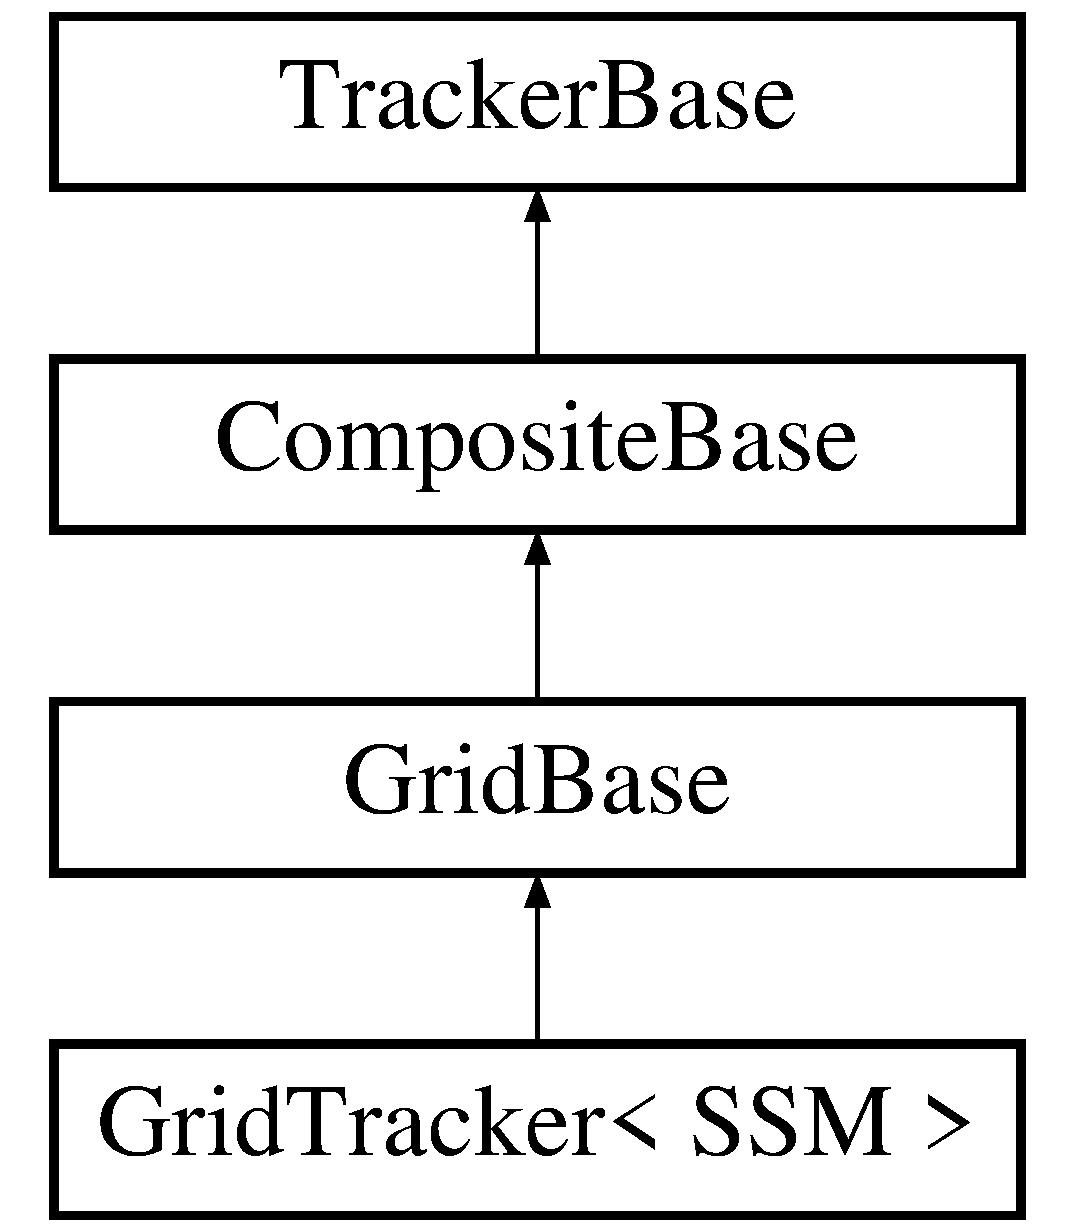
\includegraphics[height=4.000000cm]{classGridTracker}
\end{center}
\end{figure}
\subsection*{Public Types}
\begin{DoxyCompactItemize}
\item 
\hypertarget{classGridTracker_a6d6d95f72d9cdd6d71a774d962d31b05}{typedef S\-S\-M\-::\-Param\-Type {\bfseries S\-S\-M\-Params}}\label{classGridTracker_a6d6d95f72d9cdd6d71a774d962d31b05}

\item 
\hypertarget{classGridTracker_ae46588aa72d85366d39646143d9334f9}{typedef S\-S\-M\-::\-Estimator\-Params {\bfseries Estimator\-Params}}\label{classGridTracker_ae46588aa72d85366d39646143d9334f9}

\item 
\hypertarget{classGridTracker_ab195f9f5ab65de67e4eb9ff58d684c02}{typedef \hyperlink{structGridTrackerParams}{Grid\-Tracker\-Params} {\bfseries Param\-Type}}\label{classGridTracker_ab195f9f5ab65de67e4eb9ff58d684c02}

\end{DoxyCompactItemize}
\subsection*{Public Member Functions}
\begin{DoxyCompactItemize}
\item 
\hypertarget{classGridTracker_a6065b5355c9cf487a8ea792fe9ff3853}{{\bfseries Grid\-Tracker} (const vector$<$ Tracker\-Base $\ast$ $>$ \-\_\-trackers, const \hyperlink{structGridTrackerParams}{Param\-Type} $\ast$grid\-\_\-params, const Estimator\-Params $\ast$\-\_\-est\-\_\-params, const \hyperlink{structSSMParams}{S\-S\-M\-Params} $\ast$ssm\-\_\-params)}\label{classGridTracker_a6065b5355c9cf487a8ea792fe9ff3853}

\item 
\hypertarget{classGridTracker_a6a960a1b2eb3929890c8658026dc8886}{void {\bfseries initialize} (const cv\-::\-Mat \&corners) override}\label{classGridTracker_a6a960a1b2eb3929890c8658026dc8886}

\item 
\hypertarget{classGridTracker_afeb93151e74fc1d6c3c233ac59634482}{void {\bfseries update} () override}\label{classGridTracker_afeb93151e74fc1d6c3c233ac59634482}

\item 
\hypertarget{classGridTracker_a43191bbe675287dca403c6369689040b}{void {\bfseries set\-Image} (const cv\-::\-Mat \&img) override}\label{classGridTracker_a43191bbe675287dca403c6369689040b}

\item 
\hypertarget{classGridTracker_a7e8f8460f269d89da0ffe6de94052fb7}{void {\bfseries set\-Region} (const cv\-::\-Mat \&corners) override}\label{classGridTracker_a7e8f8460f269d89da0ffe6de94052fb7}

\item 
\hypertarget{classGridTracker_a5b38060ac41e9d231761645217354c21}{const cv\-::\-Mat \& {\bfseries get\-Region} () override}\label{classGridTracker_a5b38060ac41e9d231761645217354c21}

\item 
\hypertarget{classGridTracker_a5ae3964ff089b564b1ae8ce66461dbce}{const uchar $\ast$ {\bfseries get\-Pix\-Mask} () override}\label{classGridTracker_a5ae3964ff089b564b1ae8ce66461dbce}

\item 
\hypertarget{classGridTracker_a96f6c677416ecf84bdefe138a91226f4}{int {\bfseries get\-Res\-X} () override}\label{classGridTracker_a96f6c677416ecf84bdefe138a91226f4}

\item 
\hypertarget{classGridTracker_aaa2642c417100ea497263d15e28a882d}{int {\bfseries get\-Res\-Y} () override}\label{classGridTracker_aaa2642c417100ea497263d15e28a882d}

\end{DoxyCompactItemize}
\subsection*{Additional Inherited Members}


The documentation for this class was generated from the following file\-:\begin{DoxyCompactItemize}
\item 
S\-M/include/mtf/\-S\-M/Grid\-Tracker.\-h\end{DoxyCompactItemize}

\hypertarget{classGridTrackerCV}{\section{Grid\-Tracker\-C\-V$<$ S\-S\-M $>$ Class Template Reference}
\label{classGridTrackerCV}\index{Grid\-Tracker\-C\-V$<$ S\-S\-M $>$@{Grid\-Tracker\-C\-V$<$ S\-S\-M $>$}}
}
Inheritance diagram for Grid\-Tracker\-C\-V$<$ S\-S\-M $>$\-:\begin{figure}[H]
\begin{center}
\leavevmode
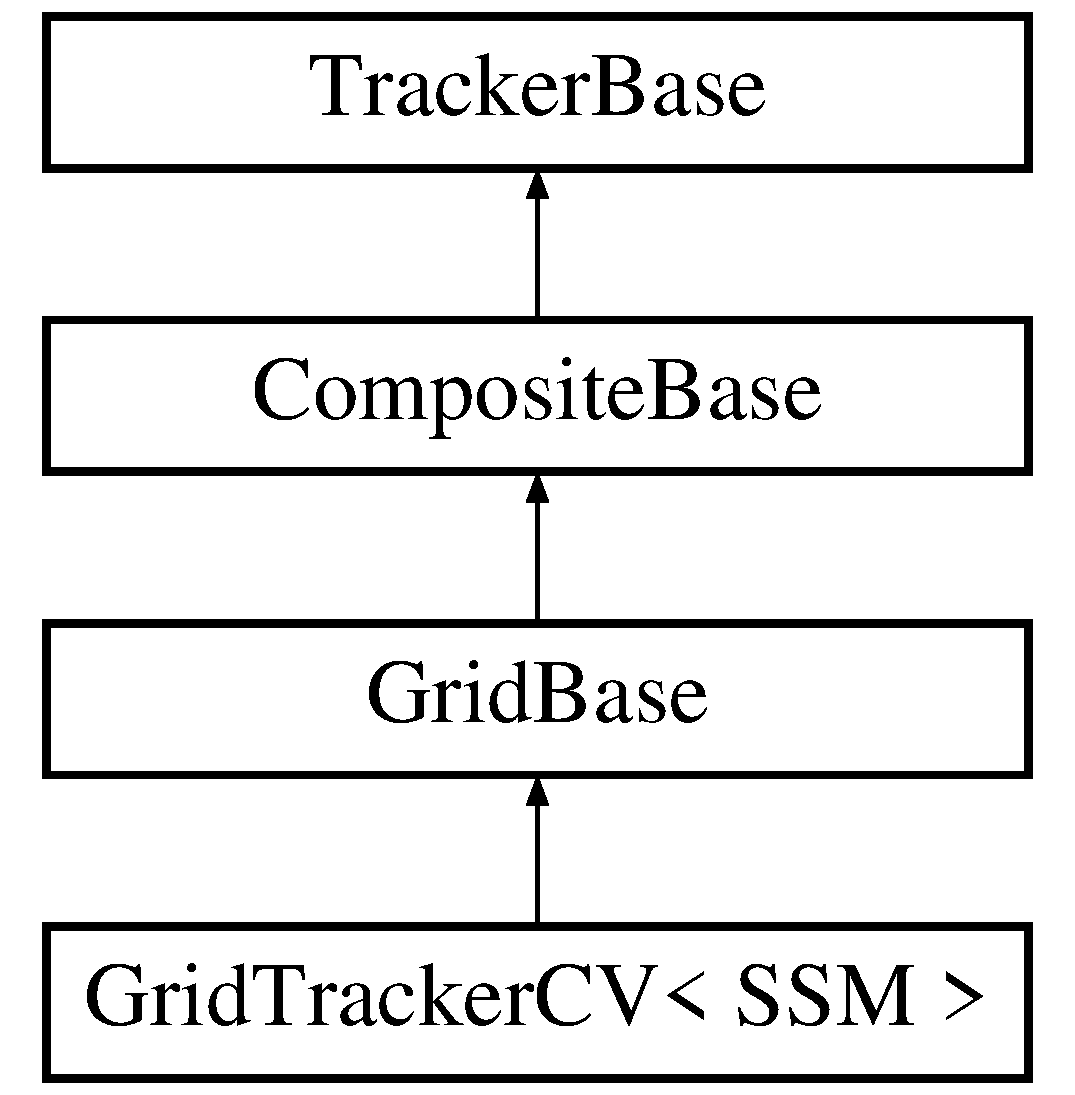
\includegraphics[height=4.000000cm]{classGridTrackerCV}
\end{center}
\end{figure}
\subsection*{Public Types}
\begin{DoxyCompactItemize}
\item 
\hypertarget{classGridTrackerCV_ac7e3185b1f9865e5bff70a1f0ff03c50}{typedef \hyperlink{structGridTrackerCVParams}{Grid\-Tracker\-C\-V\-Params} {\bfseries Param\-Type}}\label{classGridTrackerCV_ac7e3185b1f9865e5bff70a1f0ff03c50}

\item 
\hypertarget{classGridTrackerCV_a520107d545de7def984e16b6fcf7432b}{typedef S\-S\-M\-::\-Param\-Type {\bfseries S\-S\-M\-Params}}\label{classGridTrackerCV_a520107d545de7def984e16b6fcf7432b}

\item 
\hypertarget{classGridTrackerCV_a8e1ad111aa30be76a1efce6a948b9e35}{typedef S\-S\-M\-::\-Estimator\-Params {\bfseries Estimator\-Params}}\label{classGridTrackerCV_a8e1ad111aa30be76a1efce6a948b9e35}

\end{DoxyCompactItemize}
\subsection*{Public Member Functions}
\begin{DoxyCompactItemize}
\item 
\hypertarget{classGridTrackerCV_a24a98276b105cef067cd6bac3965df3d}{{\bfseries Grid\-Tracker\-C\-V} (const \hyperlink{structGridTrackerCVParams}{Param\-Type} $\ast$grid\-\_\-params, const Estimator\-Params $\ast$\-\_\-est\-\_\-params, const \hyperlink{structSSMParams}{S\-S\-M\-Params} $\ast$ssm\-\_\-params)}\label{classGridTrackerCV_a24a98276b105cef067cd6bac3965df3d}

\item 
\hypertarget{classGridTrackerCV_acc0a38caa5292351e0e9fca6da78a67f}{void {\bfseries initialize} (const cv\-::\-Mat \&corners) override}\label{classGridTrackerCV_acc0a38caa5292351e0e9fca6da78a67f}

\item 
\hypertarget{classGridTrackerCV_a9b836b5f5ad8c708e1adac18cba51967}{void {\bfseries update} () override}\label{classGridTrackerCV_a9b836b5f5ad8c708e1adac18cba51967}

\item 
\hypertarget{classGridTrackerCV_ac1c38cfe408d17ea08f862872be01b38}{void {\bfseries set\-Image} (const cv\-::\-Mat \&img) override}\label{classGridTrackerCV_ac1c38cfe408d17ea08f862872be01b38}

\item 
\hypertarget{classGridTrackerCV_aef8f7321456ff761f9f71c24bebc13b1}{void {\bfseries set\-Region} (const cv\-::\-Mat \&corners) override}\label{classGridTrackerCV_aef8f7321456ff761f9f71c24bebc13b1}

\item 
\hypertarget{classGridTrackerCV_aecc4a18455b63bf7781e898e5398fd9a}{const uchar $\ast$ {\bfseries get\-Pix\-Mask} () override}\label{classGridTrackerCV_aecc4a18455b63bf7781e898e5398fd9a}

\item 
\hypertarget{classGridTrackerCV_ace18986527c37c645f3b7cbd169ece45}{int {\bfseries get\-Res\-X} () override}\label{classGridTrackerCV_ace18986527c37c645f3b7cbd169ece45}

\item 
\hypertarget{classGridTrackerCV_aac28caa2d87bc703691bf4ddc452cb00}{int {\bfseries get\-Res\-Y} () override}\label{classGridTrackerCV_aac28caa2d87bc703691bf4ddc452cb00}

\item 
\hypertarget{classGridTrackerCV_ac05e7cff4c180363f2761cbac3a35637}{const cv\-::\-Mat \& {\bfseries get\-Region} () override}\label{classGridTrackerCV_ac05e7cff4c180363f2761cbac3a35637}

\item 
\hypertarget{classGridTrackerCV_aad9e44ba4689e55edb85ccd17ceadd3c}{int {\bfseries input\-Type} () const override}\label{classGridTrackerCV_aad9e44ba4689e55edb85ccd17ceadd3c}

\end{DoxyCompactItemize}
\subsection*{Additional Inherited Members}


The documentation for this class was generated from the following file\-:\begin{DoxyCompactItemize}
\item 
S\-M/include/mtf/\-S\-M/Grid\-Tracker\-C\-V.\-h\end{DoxyCompactItemize}

\hypertarget{structGridTrackerCVParams}{\section{Grid\-Tracker\-C\-V\-Params Struct Reference}
\label{structGridTrackerCVParams}\index{Grid\-Tracker\-C\-V\-Params@{Grid\-Tracker\-C\-V\-Params}}
}
\subsection*{Public Member Functions}
\begin{DoxyCompactItemize}
\item 
\hyperlink{structGridTrackerCVParams_a3f50b3a3d6fc9be0708503e6c853fff4}{Grid\-Tracker\-C\-V\-Params} (int \-\_\-grid\-\_\-size\-\_\-x, int \-\_\-grid\-\_\-size\-\_\-y, int \-\_\-search\-\_\-window\-\_\-x, int \-\_\-search\-\_\-window\-\_\-y, int \-\_\-pyramid\-\_\-levels, bool \-\_\-use\-\_\-min\-\_\-eig\-\_\-vals, double \-\_\-min\-\_\-eig\-\_\-thresh, int \-\_\-max\-\_\-iters, double \-\_\-epsilon, bool \-\_\-show\-\_\-trackers, bool \-\_\-debug\-\_\-mode)
\begin{DoxyCompactList}\small\item\em decides whether logging data will be printed for debugging purposes; \end{DoxyCompactList}\item 
\hypertarget{structGridTrackerCVParams_ab4caf7846c035ac58ce494dc160f670c}{{\bfseries Grid\-Tracker\-C\-V\-Params} (const \hyperlink{structGridTrackerCVParams}{Grid\-Tracker\-C\-V\-Params} $\ast$params=nullptr)}\label{structGridTrackerCVParams_ab4caf7846c035ac58ce494dc160f670c}

\item 
\hypertarget{structGridTrackerCVParams_a2c74f101f8f42405c52c4a6230494d7a}{int {\bfseries get\-Res\-X} () const }\label{structGridTrackerCVParams_a2c74f101f8f42405c52c4a6230494d7a}

\item 
\hypertarget{structGridTrackerCVParams_a60859080f03d85bf3aca3185ed34ec1f}{int {\bfseries get\-Res\-Y} () const }\label{structGridTrackerCVParams_a60859080f03d85bf3aca3185ed34ec1f}

\end{DoxyCompactItemize}
\subsection*{Public Attributes}
\begin{DoxyCompactItemize}
\item 
\hypertarget{structGridTrackerCVParams_aba0fdd206f2671cdee3239169820c6af}{int {\bfseries grid\-\_\-size\-\_\-x}}\label{structGridTrackerCVParams_aba0fdd206f2671cdee3239169820c6af}

\item 
\hypertarget{structGridTrackerCVParams_af97c06d31d7d193758b2eb30ebadfbd5}{int {\bfseries grid\-\_\-size\-\_\-y}}\label{structGridTrackerCVParams_af97c06d31d7d193758b2eb30ebadfbd5}

\item 
\hypertarget{structGridTrackerCVParams_a3dd68c8bdb2c0696b8036b6af1bab1bf}{int {\bfseries search\-\_\-window\-\_\-x}}\label{structGridTrackerCVParams_a3dd68c8bdb2c0696b8036b6af1bab1bf}

\item 
\hypertarget{structGridTrackerCVParams_a603961956091ca35a960da7468c68337}{int {\bfseries search\-\_\-window\-\_\-y}}\label{structGridTrackerCVParams_a603961956091ca35a960da7468c68337}

\item 
\hypertarget{structGridTrackerCVParams_a078d10b33e71b826cf09e7520ca17eb4}{int {\bfseries pyramid\-\_\-levels}}\label{structGridTrackerCVParams_a078d10b33e71b826cf09e7520ca17eb4}

\item 
\hypertarget{structGridTrackerCVParams_a881cd71cc37fe88ed392ead78ab924fd}{bool {\bfseries use\-\_\-min\-\_\-eig\-\_\-vals}}\label{structGridTrackerCVParams_a881cd71cc37fe88ed392ead78ab924fd}

\item 
\hypertarget{structGridTrackerCVParams_ac9490359ecd9ad3264c9a39077c7644f}{double {\bfseries min\-\_\-eig\-\_\-thresh}}\label{structGridTrackerCVParams_ac9490359ecd9ad3264c9a39077c7644f}

\item 
\hypertarget{structGridTrackerCVParams_a4e7a5aa481c382dd9c93e84ce6ebd096}{int {\bfseries max\-\_\-iters}}\label{structGridTrackerCVParams_a4e7a5aa481c382dd9c93e84ce6ebd096}

\item 
\hypertarget{structGridTrackerCVParams_a4f149d619e8b63833fa981d7af5b9c0d}{double \hyperlink{structGridTrackerCVParams_a4f149d619e8b63833fa981d7af5b9c0d}{epsilon}}\label{structGridTrackerCVParams_a4f149d619e8b63833fa981d7af5b9c0d}

\begin{DoxyCompactList}\small\item\em maximum iterations of the \hyperlink{classGridTrackerCV}{Grid\-Tracker\-C\-V} algorithm to run for each frame \end{DoxyCompactList}\item 
\hypertarget{structGridTrackerCVParams_a5d66f04ffdaeee1bb235ea2e36b2a42e}{bool {\bfseries show\-\_\-trackers}}\label{structGridTrackerCVParams_a5d66f04ffdaeee1bb235ea2e36b2a42e}

\item 
\hypertarget{structGridTrackerCVParams_a6c68435d10dbd3705e4c0848f1130489}{bool {\bfseries debug\-\_\-mode}}\label{structGridTrackerCVParams_a6c68435d10dbd3705e4c0848f1130489}

\end{DoxyCompactItemize}


\subsection{Constructor \& Destructor Documentation}
\hypertarget{structGridTrackerCVParams_a3f50b3a3d6fc9be0708503e6c853fff4}{\index{Grid\-Tracker\-C\-V\-Params@{Grid\-Tracker\-C\-V\-Params}!Grid\-Tracker\-C\-V\-Params@{Grid\-Tracker\-C\-V\-Params}}
\index{Grid\-Tracker\-C\-V\-Params@{Grid\-Tracker\-C\-V\-Params}!GridTrackerCVParams@{Grid\-Tracker\-C\-V\-Params}}
\subsubsection[{Grid\-Tracker\-C\-V\-Params}]{\setlength{\rightskip}{0pt plus 5cm}Grid\-Tracker\-C\-V\-Params\-::\-Grid\-Tracker\-C\-V\-Params (
\begin{DoxyParamCaption}
\item[{int}]{\-\_\-grid\-\_\-size\-\_\-x, }
\item[{int}]{\-\_\-grid\-\_\-size\-\_\-y, }
\item[{int}]{\-\_\-search\-\_\-window\-\_\-x, }
\item[{int}]{\-\_\-search\-\_\-window\-\_\-y, }
\item[{int}]{\-\_\-pyramid\-\_\-levels, }
\item[{bool}]{\-\_\-use\-\_\-min\-\_\-eig\-\_\-vals, }
\item[{double}]{\-\_\-min\-\_\-eig\-\_\-thresh, }
\item[{int}]{\-\_\-max\-\_\-iters, }
\item[{double}]{\-\_\-epsilon, }
\item[{bool}]{\-\_\-show\-\_\-trackers, }
\item[{bool}]{\-\_\-debug\-\_\-mode}
\end{DoxyParamCaption}
)}}\label{structGridTrackerCVParams_a3f50b3a3d6fc9be0708503e6c853fff4}


decides whether logging data will be printed for debugging purposes; 

only matters if logging is enabled at compile time 

The documentation for this struct was generated from the following file\-:\begin{DoxyCompactItemize}
\item 
S\-M/include/mtf/\-S\-M/Grid\-Tracker\-C\-V.\-h\end{DoxyCompactItemize}

\hypertarget{structGridTrackerParams}{\section{Grid\-Tracker\-Params Struct Reference}
\label{structGridTrackerParams}\index{Grid\-Tracker\-Params@{Grid\-Tracker\-Params}}
}
\subsection*{Public Member Functions}
\begin{DoxyCompactItemize}
\item 
\hyperlink{structGridTrackerParams_a909407a7a008e4b02a83eda24eef748c}{Grid\-Tracker\-Params} (int \-\_\-grid\-\_\-size\-\_\-x, int \-\_\-grid\-\_\-size\-\_\-y, int \-\_\-patch\-\_\-size\-\_\-x, int \-\_\-patch\-\_\-size\-\_\-y, bool \-\_\-init\-\_\-at\-\_\-each\-\_\-frame, bool \-\_\-dyn\-\_\-patch\-\_\-size, bool \-\_\-use\-\_\-tbb, int \-\_\-max\-\_\-iters, double \-\_\-epsilon, bool \-\_\-enable\-\_\-pyr, bool \-\_\-show\-\_\-trackers, bool \-\_\-show\-\_\-tracker\-\_\-edges, bool \-\_\-debug\-\_\-mode)
\begin{DoxyCompactList}\small\item\em decides whether logging data will be printed for debugging purposes; \end{DoxyCompactList}\item 
\hypertarget{structGridTrackerParams_a3fd4e79f4ce89397f6239ff1658a80dd}{{\bfseries Grid\-Tracker\-Params} (const \hyperlink{structGridTrackerParams}{Grid\-Tracker\-Params} $\ast$params=nullptr)}\label{structGridTrackerParams_a3fd4e79f4ce89397f6239ff1658a80dd}

\item 
\hypertarget{structGridTrackerParams_ac001ebdaf16625b4ef34b17dc2aea24f}{int {\bfseries get\-Res\-X} () const }\label{structGridTrackerParams_ac001ebdaf16625b4ef34b17dc2aea24f}

\item 
\hypertarget{structGridTrackerParams_a26dec741dd46de003cecf0c00c25d1ce}{int {\bfseries get\-Res\-Y} () const }\label{structGridTrackerParams_a26dec741dd46de003cecf0c00c25d1ce}

\end{DoxyCompactItemize}
\subsection*{Public Attributes}
\begin{DoxyCompactItemize}
\item 
\hypertarget{structGridTrackerParams_a939821b8e3e1a12dc389e61d8d5143b0}{int {\bfseries grid\-\_\-size\-\_\-x}}\label{structGridTrackerParams_a939821b8e3e1a12dc389e61d8d5143b0}

\item 
\hypertarget{structGridTrackerParams_ae30a42bcc635ea541eb9bc2d6854d089}{int {\bfseries grid\-\_\-size\-\_\-y}}\label{structGridTrackerParams_ae30a42bcc635ea541eb9bc2d6854d089}

\item 
\hypertarget{structGridTrackerParams_a7568ecb2b2b8ff9e11deefec5f6958b3}{int {\bfseries patch\-\_\-size\-\_\-x}}\label{structGridTrackerParams_a7568ecb2b2b8ff9e11deefec5f6958b3}

\item 
\hypertarget{structGridTrackerParams_ae4f66028dfd208bece8e3de315a7a557}{int {\bfseries patch\-\_\-size\-\_\-y}}\label{structGridTrackerParams_ae4f66028dfd208bece8e3de315a7a557}

\item 
\hypertarget{structGridTrackerParams_a7ac236a36e4e5479a7ccfa6fa2f228dc}{bool {\bfseries init\-\_\-at\-\_\-each\-\_\-frame}}\label{structGridTrackerParams_a7ac236a36e4e5479a7ccfa6fa2f228dc}

\item 
\hypertarget{structGridTrackerParams_a2dc8d87f746652a1f520b26348a0c61a}{bool {\bfseries dyn\-\_\-patch\-\_\-size}}\label{structGridTrackerParams_a2dc8d87f746652a1f520b26348a0c61a}

\item 
\hypertarget{structGridTrackerParams_aa86f08fe2ecd32b1be5d6e7a7bbb0bb0}{bool {\bfseries use\-\_\-tbb}}\label{structGridTrackerParams_aa86f08fe2ecd32b1be5d6e7a7bbb0bb0}

\item 
\hypertarget{structGridTrackerParams_a44d9ae3ebc1b9d6aba169a312ca9d9ec}{int {\bfseries max\-\_\-iters}}\label{structGridTrackerParams_a44d9ae3ebc1b9d6aba169a312ca9d9ec}

\item 
\hypertarget{structGridTrackerParams_a9399202ce3d29dc34b2bad622c0e438f}{double \hyperlink{structGridTrackerParams_a9399202ce3d29dc34b2bad622c0e438f}{epsilon}}\label{structGridTrackerParams_a9399202ce3d29dc34b2bad622c0e438f}

\begin{DoxyCompactList}\small\item\em maximum iterations of the \hyperlink{classGridTracker}{Grid\-Tracker} algorithm to run for each frame \end{DoxyCompactList}\item 
\hypertarget{structGridTrackerParams_a0516980c61b4f4915e44c54384cc9446}{bool {\bfseries enable\-\_\-pyr}}\label{structGridTrackerParams_a0516980c61b4f4915e44c54384cc9446}

\item 
\hypertarget{structGridTrackerParams_a965b5f1d03e9d7311a2e899ef8d41f13}{bool {\bfseries show\-\_\-trackers}}\label{structGridTrackerParams_a965b5f1d03e9d7311a2e899ef8d41f13}

\item 
\hypertarget{structGridTrackerParams_ae8bd52af8dfc1dc39c6b6247645a72ae}{bool {\bfseries show\-\_\-tracker\-\_\-edges}}\label{structGridTrackerParams_ae8bd52af8dfc1dc39c6b6247645a72ae}

\item 
\hypertarget{structGridTrackerParams_ae52fc0ee24d84c603b68f1da419bb731}{bool {\bfseries debug\-\_\-mode}}\label{structGridTrackerParams_ae52fc0ee24d84c603b68f1da419bb731}

\end{DoxyCompactItemize}


\subsection{Constructor \& Destructor Documentation}
\hypertarget{structGridTrackerParams_a909407a7a008e4b02a83eda24eef748c}{\index{Grid\-Tracker\-Params@{Grid\-Tracker\-Params}!Grid\-Tracker\-Params@{Grid\-Tracker\-Params}}
\index{Grid\-Tracker\-Params@{Grid\-Tracker\-Params}!GridTrackerParams@{Grid\-Tracker\-Params}}
\subsubsection[{Grid\-Tracker\-Params}]{\setlength{\rightskip}{0pt plus 5cm}Grid\-Tracker\-Params\-::\-Grid\-Tracker\-Params (
\begin{DoxyParamCaption}
\item[{int}]{\-\_\-grid\-\_\-size\-\_\-x, }
\item[{int}]{\-\_\-grid\-\_\-size\-\_\-y, }
\item[{int}]{\-\_\-patch\-\_\-size\-\_\-x, }
\item[{int}]{\-\_\-patch\-\_\-size\-\_\-y, }
\item[{bool}]{\-\_\-init\-\_\-at\-\_\-each\-\_\-frame, }
\item[{bool}]{\-\_\-dyn\-\_\-patch\-\_\-size, }
\item[{bool}]{\-\_\-use\-\_\-tbb, }
\item[{int}]{\-\_\-max\-\_\-iters, }
\item[{double}]{\-\_\-epsilon, }
\item[{bool}]{\-\_\-enable\-\_\-pyr, }
\item[{bool}]{\-\_\-show\-\_\-trackers, }
\item[{bool}]{\-\_\-show\-\_\-tracker\-\_\-edges, }
\item[{bool}]{\-\_\-debug\-\_\-mode}
\end{DoxyParamCaption}
)}}\label{structGridTrackerParams_a909407a7a008e4b02a83eda24eef748c}


decides whether logging data will be printed for debugging purposes; 

only matters if logging is enabled at compile time 

The documentation for this struct was generated from the following file\-:\begin{DoxyCompactItemize}
\item 
S\-M/include/mtf/\-S\-M/Grid\-Tracker.\-h\end{DoxyCompactItemize}

\hypertarget{classHACLK}{\section{H\-A\-C\-L\-K$<$ A\-M, S\-S\-M $>$ Class Template Reference}
\label{classHACLK}\index{H\-A\-C\-L\-K$<$ A\-M, S\-S\-M $>$@{H\-A\-C\-L\-K$<$ A\-M, S\-S\-M $>$}}
}
Inheritance diagram for H\-A\-C\-L\-K$<$ A\-M, S\-S\-M $>$\-:\begin{figure}[H]
\begin{center}
\leavevmode
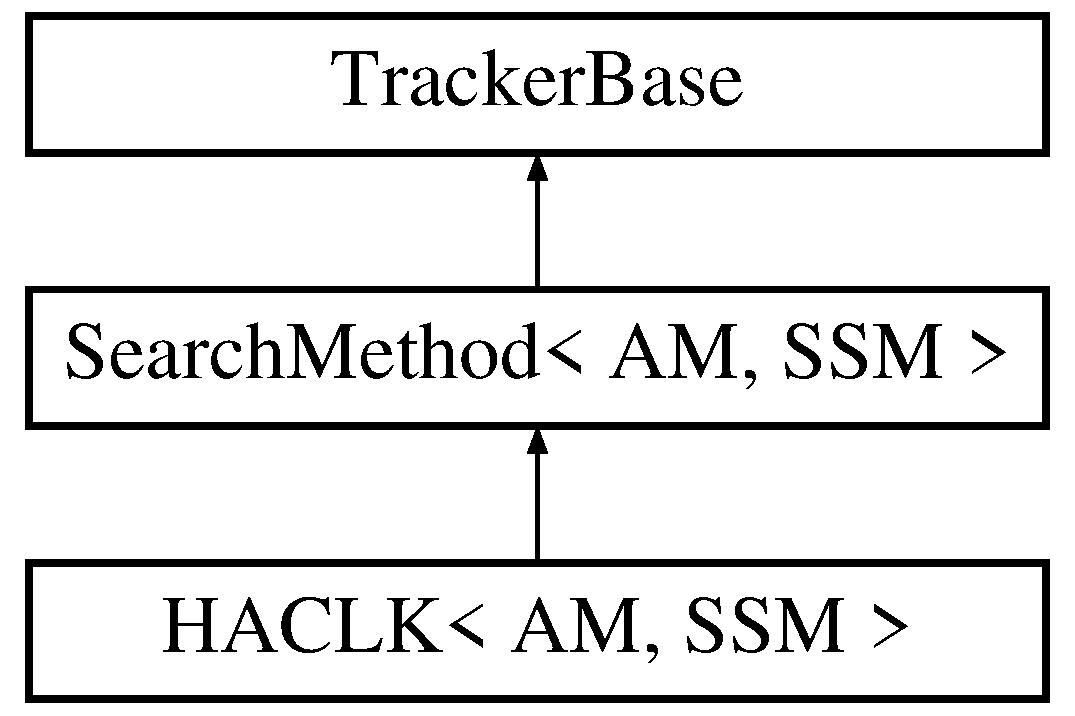
\includegraphics[height=3.000000cm]{classHACLK}
\end{center}
\end{figure}
\subsection*{Public Types}
\begin{DoxyCompactItemize}
\item 
enum \{ \\*
{\bfseries Gauss\-Newton}, 
{\bfseries Newton}, 
{\bfseries Initial\-Newton}, 
{\bfseries Current\-Newton}, 
\\*
{\bfseries Converged\-Newton}
 \}
\item 
\hypertarget{classHACLK_aea5c88e5ed26c6b5f3914dd6a333535e}{typedef \hyperlink{structHACLKParams}{H\-A\-C\-L\-K\-Params} {\bfseries Param\-Type}}\label{classHACLK_aea5c88e5ed26c6b5f3914dd6a333535e}

\end{DoxyCompactItemize}
\subsection*{Public Member Functions}
\begin{DoxyCompactItemize}
\item 
\hypertarget{classHACLK_af2729c6008639b5009212214780a5899}{{\bfseries H\-A\-C\-L\-K} (const \hyperlink{structHACLKParams}{Param\-Type} $\ast$haclk\-\_\-params=nullptr, const \hyperlink{structAMParams}{A\-M\-Params} $\ast$am\-\_\-params=nullptr, const \hyperlink{structSSMParams}{S\-S\-M\-Params} $\ast$ssm\-\_\-params=nullptr)}\label{classHACLK_af2729c6008639b5009212214780a5899}

\item 
\hypertarget{classHACLK_ab2ebdfe87be6bd27d88e64739b6287b1}{void {\bfseries initialize} (const cv\-::\-Mat \&corners) override}\label{classHACLK_ab2ebdfe87be6bd27d88e64739b6287b1}

\item 
\hypertarget{classHACLK_aee3c321d63b71822ed51fcec04b219e5}{void {\bfseries update} () override}\label{classHACLK_aee3c321d63b71822ed51fcec04b219e5}

\end{DoxyCompactItemize}
\subsection*{Public Attributes}
\begin{DoxyCompactItemize}
\item 
\hypertarget{classHACLK_ac8db1e67d533f067fa907f62d092371a}{bool {\bfseries use\-\_\-newton\-\_\-method}}\label{classHACLK_ac8db1e67d533f067fa907f62d092371a}

\item 
\hypertarget{classHACLK_ab2d257d242d7ed7fc99ab0f67636fe62}{\hyperlink{structHACLKParams}{Param\-Type} {\bfseries params}}\label{classHACLK_ab2d257d242d7ed7fc99ab0f67636fe62}

\item 
\hypertarget{classHACLK_af4af6fad4891e79604874024c219afd6}{Matrix\-Xd \hyperlink{classHACLK_af4af6fad4891e79604874024c219afd6}{init\-\_\-pix\-\_\-jacobian}}\label{classHACLK_af4af6fad4891e79604874024c219afd6}

\begin{DoxyCompactList}\small\item\em N x S jacobians of the pix values w.\-r.\-t the S\-S\-M state vector. \end{DoxyCompactList}\item 
\hypertarget{classHACLK_af9a83d6bd6f0c9a28e1fa55566467f52}{Matrix\-Xd {\bfseries curr\-\_\-pix\-\_\-jacobian}}\label{classHACLK_af9a83d6bd6f0c9a28e1fa55566467f52}

\item 
\hypertarget{classHACLK_a6375da2cc74b787e142e5940c6691b68}{Matrix\-Xd \hyperlink{classHACLK_a6375da2cc74b787e142e5940c6691b68}{init\-\_\-pix\-\_\-hessian}}\label{classHACLK_a6375da2cc74b787e142e5940c6691b68}

\begin{DoxyCompactList}\small\item\em N x S x S hessians of the pixel values w.\-r.\-t the S\-S\-M state vector stored as a (S$\ast$\-S) x N 2\-D matrix. \end{DoxyCompactList}\item 
\hypertarget{classHACLK_a2e41b2138751bcb648148e68a6accabd}{Matrix\-Xd {\bfseries curr\-\_\-pix\-\_\-hessian}}\label{classHACLK_a2e41b2138751bcb648148e68a6accabd}

\item 
\hypertarget{classHACLK_a12cd9ed711a94382d6ae8fb04c7c7555}{Row\-Vector\-Xd \hyperlink{classHACLK_a12cd9ed711a94382d6ae8fb04c7c7555}{similarity\-\_\-jacobian}}\label{classHACLK_a12cd9ed711a94382d6ae8fb04c7c7555}

\begin{DoxyCompactList}\small\item\em 1 x S Jacobian of the A\-M error norm w.\-r.\-t. S\-S\-M state vector \end{DoxyCompactList}\item 
\hypertarget{classHACLK_a0c0831c264ccf58e1c8140541ea107ef}{Matrix\-Xd \hyperlink{classHACLK_a0c0831c264ccf58e1c8140541ea107ef}{hessian}}\label{classHACLK_a0c0831c264ccf58e1c8140541ea107ef}

\begin{DoxyCompactList}\small\item\em S x S Hessian of the A\-M error norm w.\-r.\-t. S\-S\-M state vector. \end{DoxyCompactList}\item 
\hypertarget{classHACLK_ad37d4fa90531b6db259173e108c54cb6}{Matrix24d {\bfseries curr\-\_\-conv\-\_\-corners}}\label{classHACLK_ad37d4fa90531b6db259173e108c54cb6}

\item 
\hypertarget{classHACLK_a72de22bc57f15c21013d482d46bfee61}{Matrix24d {\bfseries prev\-\_\-corners}}\label{classHACLK_a72de22bc57f15c21013d482d46bfee61}

\item 
\hypertarget{classHACLK_a589b547a4e40bb2e5a7477a2730401bd}{Vector\-Xd {\bfseries ssm\-\_\-update}}\label{classHACLK_a589b547a4e40bb2e5a7477a2730401bd}

\item 
\hypertarget{classHACLK_af0c99a7979057ee8bf1a762525d58cc5}{Matrix3d {\bfseries warp\-\_\-update}}\label{classHACLK_af0c99a7979057ee8bf1a762525d58cc5}

\item 
\hypertarget{classHACLK_ab1e939ce76a7213dd90f3b7a0cdc8050}{int {\bfseries n\-\_\-frames}}\label{classHACLK_ab1e939ce76a7213dd90f3b7a0cdc8050}

\item 
\hypertarget{classHACLK_a0c1bc94737457eccb962ef8d3f624d6f}{int {\bfseries frame\-\_\-id}}\label{classHACLK_a0c1bc94737457eccb962ef8d3f624d6f}

\end{DoxyCompactItemize}
\subsection*{Additional Inherited Members}


The documentation for this class was generated from the following file\-:\begin{DoxyCompactItemize}
\item 
S\-M/include/mtf/\-S\-M/H\-A\-C\-L\-K.\-h\end{DoxyCompactItemize}

\hypertarget{structHACLKParams}{\section{H\-A\-C\-L\-K\-Params Struct Reference}
\label{structHACLKParams}\index{H\-A\-C\-L\-K\-Params@{H\-A\-C\-L\-K\-Params}}
}
\subsection*{Public Member Functions}
\begin{DoxyCompactItemize}
\item 
\hypertarget{structHACLKParams_acbfc280437f95b4efe7627bedcbc2362}{{\bfseries H\-A\-C\-L\-K\-Params} (int \-\_\-max\-\_\-iters, double \-\_\-epsilon, bool \-\_\-rec\-\_\-init\-\_\-err\-\_\-grad, bool \-\_\-debug\-\_\-mode, int \-\_\-hess\-\_\-type, const std\-::vector$<$ cv\-::\-Mat $>$ \&\-\_\-converged\-\_\-corners)}\label{structHACLKParams_acbfc280437f95b4efe7627bedcbc2362}

\item 
\hypertarget{structHACLKParams_afad3712126fc62b7a3e035f514194538}{{\bfseries H\-A\-C\-L\-K\-Params} (\hyperlink{structHACLKParams}{H\-A\-C\-L\-K\-Params} $\ast$params=nullptr)}\label{structHACLKParams_afad3712126fc62b7a3e035f514194538}

\end{DoxyCompactItemize}
\subsection*{Public Attributes}
\begin{DoxyCompactItemize}
\item 
\hypertarget{structHACLKParams_a579e0e9dbe1c2c3c28b26ef5a16464ce}{int {\bfseries max\-\_\-iters}}\label{structHACLKParams_a579e0e9dbe1c2c3c28b26ef5a16464ce}

\item 
\hypertarget{structHACLKParams_a06bb5fb4862d6d81a97ad9432afa0e70}{double \hyperlink{structHACLKParams_a06bb5fb4862d6d81a97ad9432afa0e70}{epsilon}}\label{structHACLKParams_a06bb5fb4862d6d81a97ad9432afa0e70}

\begin{DoxyCompactList}\small\item\em maximum iterations of the \hyperlink{classHACLK}{H\-A\-C\-L\-K} algorithm to run for each frame \end{DoxyCompactList}\item 
\hypertarget{structHACLKParams_a18e6aab09bf131d48b5c7ee013fe26f0}{bool \hyperlink{structHACLKParams_a18e6aab09bf131d48b5c7ee013fe26f0}{rec\-\_\-init\-\_\-err\-\_\-grad}}\label{structHACLKParams_a18e6aab09bf131d48b5c7ee013fe26f0}

\begin{DoxyCompactList}\small\item\em maximum L1 norm of the state update vector at which to stop the iterations \end{DoxyCompactList}\item 
bool \hyperlink{structHACLKParams_ae1b1aafcc9c2b966be957699c92f228a}{debug\-\_\-mode}
\begin{DoxyCompactList}\small\item\em decides if the gradient of the error vector w.\-r.\-t. \end{DoxyCompactList}\item 
int \hyperlink{structHACLKParams_a1acbdb628145c0aedddce3c6ea0f2c74}{hess\-\_\-type}
\begin{DoxyCompactList}\small\item\em decides whether logging data will be printed for debugging purposes; \end{DoxyCompactList}\item 
\hypertarget{structHACLKParams_ace5bdabe3beadcb59289773f8eb30da5}{std\-::vector$<$ cv\-::\-Mat $>$ {\bfseries converged\-\_\-corners}}\label{structHACLKParams_ace5bdabe3beadcb59289773f8eb30da5}

\end{DoxyCompactItemize}


\subsection{Member Data Documentation}
\hypertarget{structHACLKParams_ae1b1aafcc9c2b966be957699c92f228a}{\index{H\-A\-C\-L\-K\-Params@{H\-A\-C\-L\-K\-Params}!debug\-\_\-mode@{debug\-\_\-mode}}
\index{debug\-\_\-mode@{debug\-\_\-mode}!HACLKParams@{H\-A\-C\-L\-K\-Params}}
\subsubsection[{debug\-\_\-mode}]{\setlength{\rightskip}{0pt plus 5cm}bool H\-A\-C\-L\-K\-Params\-::debug\-\_\-mode}}\label{structHACLKParams_ae1b1aafcc9c2b966be957699c92f228a}


decides if the gradient of the error vector w.\-r.\-t. 

initial pix values is recomputed every time the vector changes \hypertarget{structHACLKParams_a1acbdb628145c0aedddce3c6ea0f2c74}{\index{H\-A\-C\-L\-K\-Params@{H\-A\-C\-L\-K\-Params}!hess\-\_\-type@{hess\-\_\-type}}
\index{hess\-\_\-type@{hess\-\_\-type}!HACLKParams@{H\-A\-C\-L\-K\-Params}}
\subsubsection[{hess\-\_\-type}]{\setlength{\rightskip}{0pt plus 5cm}int H\-A\-C\-L\-K\-Params\-::hess\-\_\-type}}\label{structHACLKParams_a1acbdb628145c0aedddce3c6ea0f2c74}


decides whether logging data will be printed for debugging purposes; 

only matters if logging is enabled at compile time 

The documentation for this struct was generated from the following file\-:\begin{DoxyCompactItemize}
\item 
S\-M/include/mtf/\-S\-M/H\-A\-C\-L\-K.\-h\end{DoxyCompactItemize}

\hypertarget{classHESM}{\section{H\-E\-S\-M$<$ A\-M, S\-S\-M, S\-S\-M2 $>$ Class Template Reference}
\label{classHESM}\index{H\-E\-S\-M$<$ A\-M, S\-S\-M, S\-S\-M2 $>$@{H\-E\-S\-M$<$ A\-M, S\-S\-M, S\-S\-M2 $>$}}
}
Inheritance diagram for H\-E\-S\-M$<$ A\-M, S\-S\-M, S\-S\-M2 $>$\-:\begin{figure}[H]
\begin{center}
\leavevmode
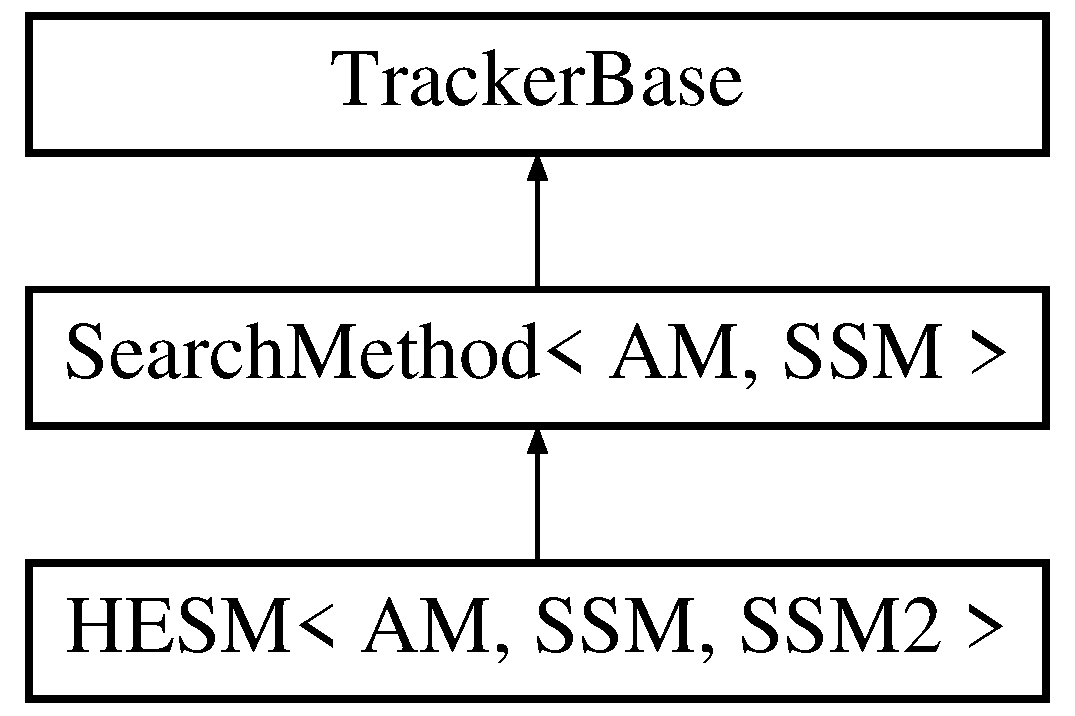
\includegraphics[height=3.000000cm]{classHESM}
\end{center}
\end{figure}
\subsection*{Public Types}
\begin{DoxyCompactItemize}
\item 
\hypertarget{classHESM_abf41db8320054f6d6832d01efa6ebf80}{typedef \hyperlink{structHESMParams}{H\-E\-S\-M\-Params} {\bfseries Param\-Type}}\label{classHESM_abf41db8320054f6d6832d01efa6ebf80}

\item 
\hypertarget{classHESM_af4b52c198e7fd03cee9524ae0d62fc7a}{typedef S\-S\-M2\-::\-Param\-Type {\bfseries S\-S\-M2\-Params}}\label{classHESM_af4b52c198e7fd03cee9524ae0d62fc7a}

\end{DoxyCompactItemize}
\subsection*{Public Member Functions}
\begin{DoxyCompactItemize}
\item 
\hypertarget{classHESM_a71c77aa3cfab2430af02a0798cbd173f}{\hyperlink{classHESM_a71c77aa3cfab2430af02a0798cbd173f}{H\-E\-S\-M} (const \hyperlink{structHESMParams}{Param\-Type} $\ast$nesm\-\_\-params=N\-U\-L\-L, const \hyperlink{structAMParams}{A\-M\-Params} $\ast$am\-\_\-params=N\-U\-L\-L, const \hyperlink{structSSMParams}{S\-S\-M\-Params} $\ast$ssm\-\_\-params=N\-U\-L\-L, S\-S\-M2\-Params $\ast$ssm2\-\_\-params=N\-U\-L\-L)}\label{classHESM_a71c77aa3cfab2430af02a0798cbd173f}

\begin{DoxyCompactList}\small\item\em A x S mean of the initial and current jacobians of the A\-M error vector w.\-r.\-t. the S\-S\-M state vector;. \end{DoxyCompactList}\item 
\hypertarget{classHESM_aa0134870cb70c8123643d425549fd2b3}{void {\bfseries initialize} (const cv\-::\-Mat \&corners)}\label{classHESM_aa0134870cb70c8123643d425549fd2b3}

\item 
\hypertarget{classHESM_a3b5036e4cbf5aa113e43ead3efb61cb1}{void {\bfseries update} ()}\label{classHESM_a3b5036e4cbf5aa113e43ead3efb61cb1}

\item 
\hypertarget{classHESM_a1c2db3ae802c81f00b0c4093612c114d}{{\footnotesize template$<$class \-\_\-\-S\-S\-M $>$ }\\void {\bfseries update\-S\-S\-M} (\-\_\-\-S\-S\-M $\ast$\-\_\-ssm, \hyperlink{structSSMData}{S\-S\-M\-Data} \&\-\_\-data)}\label{classHESM_a1c2db3ae802c81f00b0c4093612c114d}

\end{DoxyCompactItemize}
\subsection*{Public Attributes}
\begin{DoxyCompactItemize}
\item 
\hypertarget{classHESM_a87e59e57ccec4467d7745c2d99219e6e}{\hyperlink{structHESMParams}{Param\-Type} {\bfseries params}}\label{classHESM_a87e59e57ccec4467d7745c2d99219e6e}

\item 
\hypertarget{classHESM_a6c1c00ffbc289e8028529807e8c0da50}{int {\bfseries frame\-\_\-id}}\label{classHESM_a6c1c00ffbc289e8028529807e8c0da50}

\item 
\hypertarget{classHESM_ad8a37b50b1f76c6598e3c76e497d733a}{char $\ast$ {\bfseries log\-\_\-fname}}\label{classHESM_ad8a37b50b1f76c6598e3c76e497d733a}

\item 
\hypertarget{classHESM_a6dba5f327ca9a5a158b62016d19a1708}{char $\ast$ {\bfseries time\-\_\-fname}}\label{classHESM_a6dba5f327ca9a5a158b62016d19a1708}

\item 
\hypertarget{classHESM_a40cfa5c9a331cbc73050639667eb451b}{S\-S\-M2 $\ast$ {\bfseries ssm2}}\label{classHESM_a40cfa5c9a331cbc73050639667eb451b}

\item 
\hypertarget{classHESM_ab2b7017dd86f6c2cebc5e07dba545cb2}{\hyperlink{structSSMData}{S\-S\-M\-Data} {\bfseries ssm\-\_\-data}}\label{classHESM_ab2b7017dd86f6c2cebc5e07dba545cb2}

\item 
\hypertarget{classHESM_ac426f9fe32f637e70f2e2d3d8a59f7de}{\hyperlink{structSSMData}{S\-S\-M\-Data} {\bfseries ssm2\-\_\-data}}\label{classHESM_ac426f9fe32f637e70f2e2d3d8a59f7de}

\item 
\hypertarget{classHESM_a05b53b1bef8dc84572c6e10d9b7bff42}{Matrix24d {\bfseries prev\-\_\-corners}}\label{classHESM_a05b53b1bef8dc84572c6e10d9b7bff42}

\item 
Matrix3d \hyperlink{classHESM_a2528f05cea5cc5c9485a5b31a9b6d092}{ssm2\-\_\-warp\-\_\-update}
\begin{DoxyCompactList}\small\item\em N x S jacobians of the pixel values w.\-r.\-t the S\-S\-M state vector where N = resx $\ast$ resy is the no. \end{DoxyCompactList}\end{DoxyCompactItemize}
\subsection*{Additional Inherited Members}


\subsection{Member Data Documentation}
\hypertarget{classHESM_a2528f05cea5cc5c9485a5b31a9b6d092}{\index{H\-E\-S\-M@{H\-E\-S\-M}!ssm2\-\_\-warp\-\_\-update@{ssm2\-\_\-warp\-\_\-update}}
\index{ssm2\-\_\-warp\-\_\-update@{ssm2\-\_\-warp\-\_\-update}!HESM@{H\-E\-S\-M}}
\subsubsection[{ssm2\-\_\-warp\-\_\-update}]{\setlength{\rightskip}{0pt plus 5cm}template$<$class A\-M , class S\-S\-M , class S\-S\-M2 $>$ Matrix3d {\bf H\-E\-S\-M}$<$ A\-M, S\-S\-M, S\-S\-M2 $>$\-::ssm2\-\_\-warp\-\_\-update}}\label{classHESM_a2528f05cea5cc5c9485a5b31a9b6d092}


N x S jacobians of the pixel values w.\-r.\-t the S\-S\-M state vector where N = resx $\ast$ resy is the no. 

of pixels in the object patch 

The documentation for this class was generated from the following file\-:\begin{DoxyCompactItemize}
\item 
S\-M/include/mtf/\-S\-M/H\-E\-S\-M.\-h\end{DoxyCompactItemize}

\hypertarget{structHESMParams}{\section{H\-E\-S\-M\-Params Struct Reference}
\label{structHESMParams}\index{H\-E\-S\-M\-Params@{H\-E\-S\-M\-Params}}
}
\subsection*{Public Member Functions}
\begin{DoxyCompactItemize}
\item 
\hyperlink{structHESMParams_a267b8be732ff048f01159e056184133b}{H\-E\-S\-M\-Params} (int \-\_\-max\-\_\-iters, double \-\_\-epsilon, bool \-\_\-rec\-\_\-init\-\_\-err\-\_\-grad, bool \-\_\-debug\-\_\-mode)
\begin{DoxyCompactList}\small\item\em decides whether logging data will be printed for debugging purposes; \end{DoxyCompactList}\item 
\hypertarget{structHESMParams_a9a2cbc081cf02a13407be2c7595e0272}{{\bfseries H\-E\-S\-M\-Params} (\hyperlink{structHESMParams}{H\-E\-S\-M\-Params} $\ast$params=nullptr)}\label{structHESMParams_a9a2cbc081cf02a13407be2c7595e0272}

\end{DoxyCompactItemize}
\subsection*{Public Attributes}
\begin{DoxyCompactItemize}
\item 
\hypertarget{structHESMParams_aa653addbecae100fcf512b661bd09b37}{int {\bfseries max\-\_\-iters}}\label{structHESMParams_aa653addbecae100fcf512b661bd09b37}

\item 
\hypertarget{structHESMParams_af18ff4f71d9d4432b7c2089e5b646f35}{double \hyperlink{structHESMParams_af18ff4f71d9d4432b7c2089e5b646f35}{epsilon}}\label{structHESMParams_af18ff4f71d9d4432b7c2089e5b646f35}

\begin{DoxyCompactList}\small\item\em maximum iterations of the \hyperlink{classHESM}{H\-E\-S\-M} algorithm to run for each frame \end{DoxyCompactList}\item 
\hypertarget{structHESMParams_a31e31801829a257b843e260c3068caee}{bool \hyperlink{structHESMParams_a31e31801829a257b843e260c3068caee}{rec\-\_\-init\-\_\-err\-\_\-grad}}\label{structHESMParams_a31e31801829a257b843e260c3068caee}

\begin{DoxyCompactList}\small\item\em maximum L1 norm of the state update vector at which to stop the iterations \end{DoxyCompactList}\item 
bool \hyperlink{structHESMParams_ac8ef09af9c0a41d404ff03237ecb0b58}{debug\-\_\-mode}
\begin{DoxyCompactList}\small\item\em decides if the gradient of the error vector w.\-r.\-t. \end{DoxyCompactList}\end{DoxyCompactItemize}


\subsection{Constructor \& Destructor Documentation}
\hypertarget{structHESMParams_a267b8be732ff048f01159e056184133b}{\index{H\-E\-S\-M\-Params@{H\-E\-S\-M\-Params}!H\-E\-S\-M\-Params@{H\-E\-S\-M\-Params}}
\index{H\-E\-S\-M\-Params@{H\-E\-S\-M\-Params}!HESMParams@{H\-E\-S\-M\-Params}}
\subsubsection[{H\-E\-S\-M\-Params}]{\setlength{\rightskip}{0pt plus 5cm}H\-E\-S\-M\-Params\-::\-H\-E\-S\-M\-Params (
\begin{DoxyParamCaption}
\item[{int}]{\-\_\-max\-\_\-iters, }
\item[{double}]{\-\_\-epsilon, }
\item[{bool}]{\-\_\-rec\-\_\-init\-\_\-err\-\_\-grad, }
\item[{bool}]{\-\_\-debug\-\_\-mode}
\end{DoxyParamCaption}
)\hspace{0.3cm}{\ttfamily [inline]}}}\label{structHESMParams_a267b8be732ff048f01159e056184133b}


decides whether logging data will be printed for debugging purposes; 

only matters if logging is enabled at compile time 

\subsection{Member Data Documentation}
\hypertarget{structHESMParams_ac8ef09af9c0a41d404ff03237ecb0b58}{\index{H\-E\-S\-M\-Params@{H\-E\-S\-M\-Params}!debug\-\_\-mode@{debug\-\_\-mode}}
\index{debug\-\_\-mode@{debug\-\_\-mode}!HESMParams@{H\-E\-S\-M\-Params}}
\subsubsection[{debug\-\_\-mode}]{\setlength{\rightskip}{0pt plus 5cm}bool H\-E\-S\-M\-Params\-::debug\-\_\-mode}}\label{structHESMParams_ac8ef09af9c0a41d404ff03237ecb0b58}


decides if the gradient of the error vector w.\-r.\-t. 

initial pix values is recomputed every time the vector changes 

The documentation for this struct was generated from the following file\-:\begin{DoxyCompactItemize}
\item 
S\-M/include/mtf/\-S\-M/H\-E\-S\-M.\-h\end{DoxyCompactItemize}

\hypertarget{classHomography}{\section{Homography Class Reference}
\label{classHomography}\index{Homography@{Homography}}
}
Inheritance diagram for Homography\-:\begin{figure}[H]
\begin{center}
\leavevmode
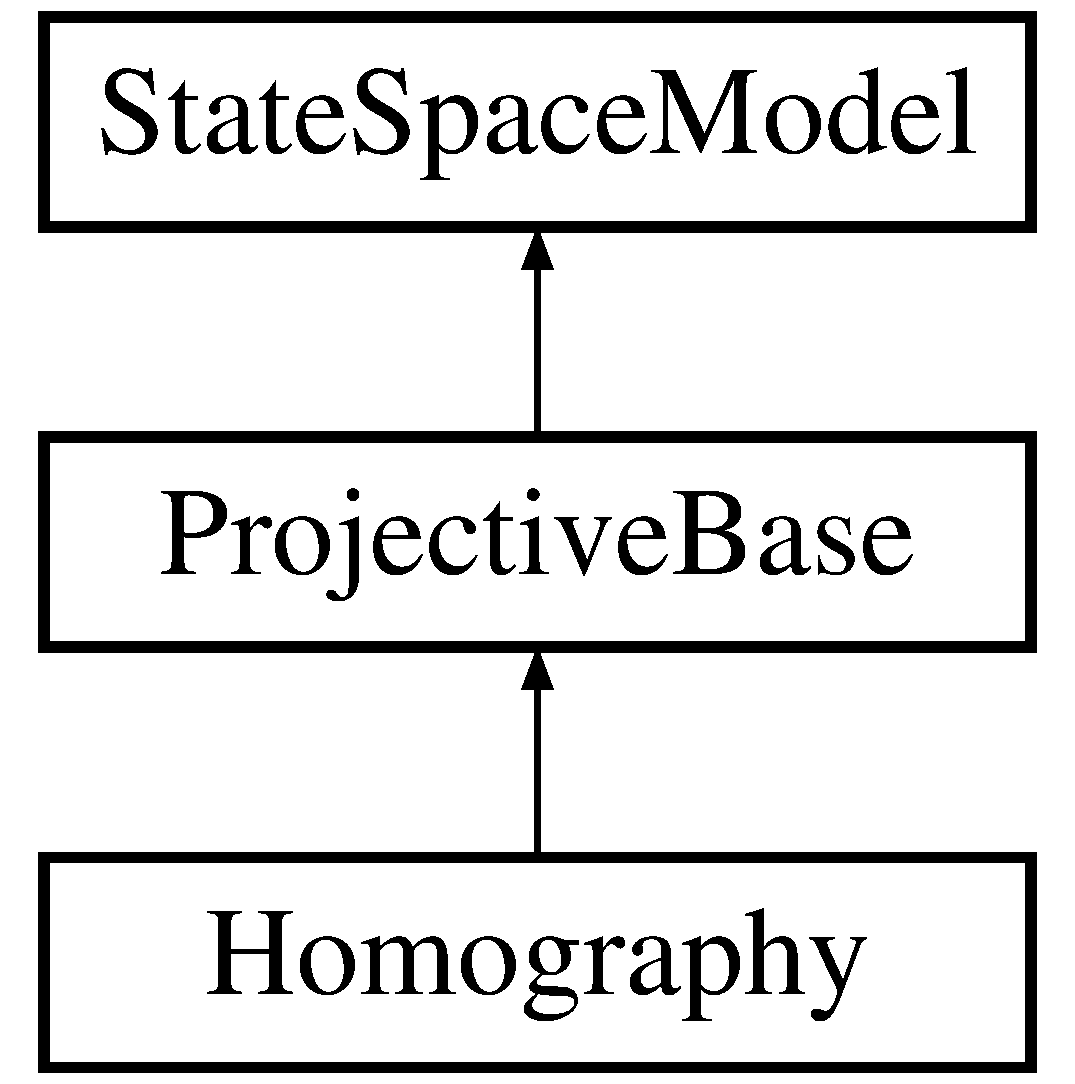
\includegraphics[height=3.000000cm]{classHomography}
\end{center}
\end{figure}
\subsection*{Public Types}
\begin{DoxyCompactItemize}
\item 
\hypertarget{classHomography_a263893666fd512975f8d6c01b1bbf8b0}{typedef \hyperlink{structHomographyParams}{Homography\-Params} {\bfseries Param\-Type}}\label{classHomography_a263893666fd512975f8d6c01b1bbf8b0}

\end{DoxyCompactItemize}
\subsection*{Public Member Functions}
\begin{DoxyCompactItemize}
\item 
\hypertarget{classHomography_a760af8a2a57d5ba53db8df6b0cc0dbe5}{{\bfseries Homography} (const \hyperlink{structHomographyParams}{Param\-Type} $\ast$params\-\_\-in=nullptr)}\label{classHomography_a760af8a2a57d5ba53db8df6b0cc0dbe5}

\item 
\hypertarget{classHomography_a5193f898d646583fbe4f7d0acde85a92}{void {\bfseries compositional\-Update} (const Vector\-Xd \&state\-\_\-update) override}\label{classHomography_a5193f898d646583fbe4f7d0acde85a92}

\item 
void \hyperlink{classHomography_a2d9bf9a73b33fe6ea5537d1ab790aa0b}{cmpt\-Init\-Pix\-Jacobian} (Matrix\-Xd \&jacobian\-\_\-prod, const Pix\-Grad\-T \&am\-\_\-jacobian) override
\begin{DoxyCompactList}\small\item\em right multiplies the initial or current ssm jacobian with the provided am jacobian; though this can be accomplished by the search method itself with simple matrix multiplication, the ssm jacobian often satisfies several constraints (e.\-g. \end{DoxyCompactList}\item 
\hypertarget{classHomography_a007cee14e5bcbed442bcf46d153b4098}{void {\bfseries cmpt\-Pix\-Jacobian} (Matrix\-Xd \&jacobian\-\_\-prod, const Pix\-Grad\-T \&am\-\_\-jacobian) override}\label{classHomography_a007cee14e5bcbed442bcf46d153b4098}

\item 
\hypertarget{classHomography_aff7a96878ef9e769f305b7f6f569cfbc}{void {\bfseries cmpt\-Warped\-Pix\-Jacobian} (Matrix\-Xd \&jacobian\-\_\-prod, const Pix\-Grad\-T \&pix\-\_\-jacobian) override}\label{classHomography_aff7a96878ef9e769f305b7f6f569cfbc}

\item 
\hypertarget{classHomography_aefda4eeb0084b101028d9fd571dcc8d4}{void {\bfseries cmpt\-Approx\-Pix\-Jacobian} (Matrix\-Xd \&jacobian\-\_\-prod, const Pix\-Grad\-T \&pix\-\_\-jacobian) override}\label{classHomography_aefda4eeb0084b101028d9fd571dcc8d4}

\item 
\hypertarget{classHomography_a828bb1018d8c7a75d45c8432d7339c79}{void {\bfseries estimate\-Warp\-From\-Corners} (Vector\-Xd \&state\-\_\-update, const Corners\-T \&in\-\_\-corners, const Corners\-T \&out\-\_\-corners) override}\label{classHomography_a828bb1018d8c7a75d45c8432d7339c79}

\item 
\hypertarget{classHomography_ab4f2300c1e237780a8f9e1785852517c}{void {\bfseries cmpt\-Init\-Pix\-Hessian} (Matrix\-Xd \&pix\-\_\-hess\-\_\-ssm, const Pix\-Hess\-T \&pix\-\_\-hess\-\_\-coord, const Pix\-Grad\-T \&pix\-\_\-grad) override}\label{classHomography_ab4f2300c1e237780a8f9e1785852517c}

\item 
\hypertarget{classHomography_ad6570e3980f5cc70afbbd27876f2a143}{void {\bfseries cmpt\-Warped\-Pix\-Hessian} (Matrix\-Xd \&pix\-\_\-hess\-\_\-ssm, const Pix\-Hess\-T \&pix\-\_\-hess\-\_\-coord, const Pix\-Grad\-T \&pix\-\_\-grad) override}\label{classHomography_ad6570e3980f5cc70afbbd27876f2a143}

\item 
\hypertarget{classHomography_ace274d1aa99394ec58cfe1a5ce52b4ef}{void {\bfseries cmpt\-Warped\-Pix\-Hessian2} (Matrix\-Xd \&pix\-\_\-hess\-\_\-ssm, const Pix\-Hess\-T \&pix\-\_\-hess\-\_\-coord, const Pix\-Grad\-T \&pix\-\_\-grad)}\label{classHomography_ace274d1aa99394ec58cfe1a5ce52b4ef}

\item 
\hypertarget{classHomography_a6fcec5bbdcdbb2956f3c42737831b135}{void {\bfseries cmpt\-Approx\-Pix\-Hessian} (Matrix\-Xd \&pix\-\_\-hess\-\_\-ssm, const Pix\-Hess\-T \&pix\-\_\-hess\-\_\-coord, const Pix\-Grad\-T \&pix\-\_\-grad) override}\label{classHomography_a6fcec5bbdcdbb2956f3c42737831b135}

\item 
\hypertarget{classHomography_ad04a9cbfcf02e00a1f400362f303304b}{void {\bfseries cmpt\-Pix\-Hessian} (Matrix\-Xd \&pix\-\_\-hess\-\_\-ssm, const Pix\-Hess\-T \&pix\-\_\-hess\-\_\-coord, const Pix\-Grad\-T \&pix\-\_\-grad) override}\label{classHomography_ad04a9cbfcf02e00a1f400362f303304b}

\item 
\hypertarget{classHomography_a1ef519ad1bbb68e0e050077cd637e98a}{void {\bfseries set\-Corners} (const Corners\-T \&corners) override}\label{classHomography_a1ef519ad1bbb68e0e050077cd637e98a}

\item 
\hypertarget{classHomography_aeda35457c9698e9274fc8917598ceb0c}{void {\bfseries estimate\-Warp\-From\-Pts} (Vector\-Xd \&state\-\_\-update, vector$<$ uchar $>$ \&mask, const vector$<$ cv\-::\-Point2f $>$ \&in\-\_\-pts, const vector$<$ cv\-::\-Point2f $>$ \&out\-\_\-pts, const \hyperlink{structSSMEstimatorParams}{Estimator\-Params} \&est\-\_\-params) override}\label{classHomography_aeda35457c9698e9274fc8917598ceb0c}

\item 
\hypertarget{classHomography_a8276bc865e1657e96904776535d20373}{void {\bfseries invert\-State} (Vector\-Xd \&inv\-\_\-state, const Vector\-Xd \&state) override}\label{classHomography_a8276bc865e1657e96904776535d20373}

\item 
\hypertarget{classHomography_af34ef3821a53ee03a51c58730df89caa}{void {\bfseries update\-Grad\-Pts} (double grad\-\_\-eps) override}\label{classHomography_af34ef3821a53ee03a51c58730df89caa}

\item 
\hypertarget{classHomography_aa643f52dbf4776b938ef6d8275f28868}{void {\bfseries update\-Hess\-Pts} (double hess\-\_\-eps) override}\label{classHomography_aa643f52dbf4776b938ef6d8275f28868}

\item 
\hypertarget{classHomography_a5fb61eb9543babcacf794e401beb3f85}{void {\bfseries get\-Init\-Pix\-Grad} (Matrix2\-Xd \&jacobian\-\_\-prod, int pix\-\_\-id) override}\label{classHomography_a5fb61eb9543babcacf794e401beb3f85}

\item 
\hypertarget{classHomography_afa185b08d4501761b64103e8b43bd89a}{void {\bfseries get\-Curr\-Pix\-Grad} (Matrix2\-Xd \&jacobian\-\_\-prod, int pix\-\_\-id) override}\label{classHomography_afa185b08d4501761b64103e8b43bd89a}

\item 
\hypertarget{classHomography_afd016ecb9b30892708b74ca8dfd58393}{void {\bfseries generate\-Perturbation} (Vector\-Xd \&state\-\_\-update) override}\label{classHomography_afd016ecb9b30892708b74ca8dfd58393}

\item 
\hypertarget{classHomography_ac1b9fd265567ea968aff9c193212ab4a}{void {\bfseries compositional\-Random\-Walk} (Vector\-Xd \&perturbed\-\_\-state, const Vector\-Xd \&base\-\_\-state) override}\label{classHomography_ac1b9fd265567ea968aff9c193212ab4a}

\item 
\hypertarget{classHomography_a5ceed5295f052323c35dc9f279b50305}{void {\bfseries compositional\-Auto\-Regression1} (Vector\-Xd \&perturbed\-\_\-state, Vector\-Xd \&perturbed\-\_\-ar, const Vector\-Xd \&base\-\_\-state, const Vector\-Xd \&base\-\_\-ar, double a=0.\-5) override}\label{classHomography_a5ceed5295f052323c35dc9f279b50305}

\item 
\hypertarget{classHomography_a7786ce0c17abd96ac09538bb56655e83}{bool {\bfseries supports\-S\-P\-I} () override}\label{classHomography_a7786ce0c17abd96ac09538bb56655e83}

\end{DoxyCompactItemize}
\subsection*{Public Attributes}
\begin{DoxyCompactItemize}
\item 
\hypertarget{classHomography_a6388afd845675fbd34a9de58655df745}{\hyperlink{structHomographyParams}{Param\-Type} {\bfseries params}}\label{classHomography_a6388afd845675fbd34a9de58655df745}

\end{DoxyCompactItemize}
\subsection*{Additional Inherited Members}


\subsection{Member Function Documentation}
\hypertarget{classHomography_a2d9bf9a73b33fe6ea5537d1ab790aa0b}{\index{Homography@{Homography}!cmpt\-Init\-Pix\-Jacobian@{cmpt\-Init\-Pix\-Jacobian}}
\index{cmpt\-Init\-Pix\-Jacobian@{cmpt\-Init\-Pix\-Jacobian}!Homography@{Homography}}
\subsubsection[{cmpt\-Init\-Pix\-Jacobian}]{\setlength{\rightskip}{0pt plus 5cm}void Homography\-::cmpt\-Init\-Pix\-Jacobian (
\begin{DoxyParamCaption}
\item[{Matrix\-Xd \&}]{jacobian\-\_\-prod, }
\item[{const Pix\-Grad\-T \&}]{pixel\-\_\-grad}
\end{DoxyParamCaption}
)\hspace{0.3cm}{\ttfamily [override]}, {\ttfamily [virtual]}}}\label{classHomography_a2d9bf9a73b33fe6ea5537d1ab790aa0b}


right multiplies the initial or current ssm jacobian with the provided am jacobian; though this can be accomplished by the search method itself with simple matrix multiplication, the ssm jacobian often satisfies several constraints (e.\-g. 

sparsity) that can be exploited to gain computational savings by manually computing the product matrix 

Reimplemented from \hyperlink{classStateSpaceModel_ac956c679581e746891c62755fe715b3b}{State\-Space\-Model}.



The documentation for this class was generated from the following file\-:\begin{DoxyCompactItemize}
\item 
S\-S\-M/include/mtf/\-S\-S\-M/Homography.\-h\end{DoxyCompactItemize}

\hypertarget{classHomographyEstimator}{\section{Homography\-Estimator Class Reference}
\label{classHomographyEstimator}\index{Homography\-Estimator@{Homography\-Estimator}}
}
Inheritance diagram for Homography\-Estimator\-:\begin{figure}[H]
\begin{center}
\leavevmode
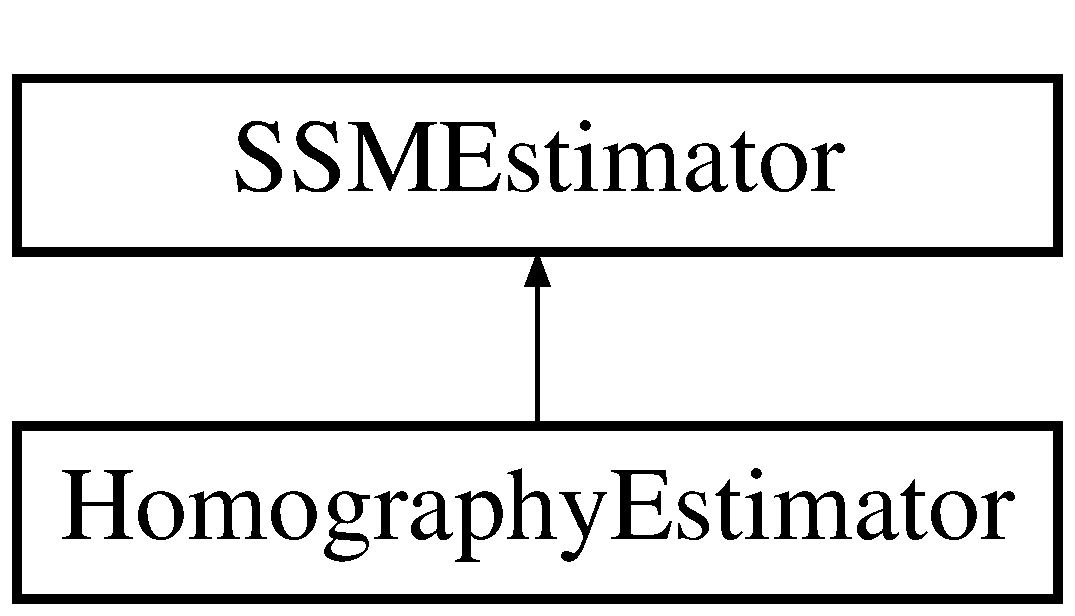
\includegraphics[height=2.000000cm]{classHomographyEstimator}
\end{center}
\end{figure}
\subsection*{Public Member Functions}
\begin{DoxyCompactItemize}
\item 
\hypertarget{classHomographyEstimator_a6b26d7a6060569953766b312a2fa057d}{{\bfseries Homography\-Estimator} (int model\-Points)}\label{classHomographyEstimator_a6b26d7a6060569953766b312a2fa057d}

\item 
\hypertarget{classHomographyEstimator_aaf252473e1eee30efe6bd716726992b5}{int {\bfseries run\-Kernel} (const Cv\-Mat $\ast$m1, const Cv\-Mat $\ast$m2, Cv\-Mat $\ast$model) override}\label{classHomographyEstimator_aaf252473e1eee30efe6bd716726992b5}

\item 
\hypertarget{classHomographyEstimator_a895f2ff605fb18992b6e4572bee51525}{bool {\bfseries refine} (const Cv\-Mat $\ast$m1, const Cv\-Mat $\ast$m2, Cv\-Mat $\ast$model, int max\-Iters) override}\label{classHomographyEstimator_a895f2ff605fb18992b6e4572bee51525}

\end{DoxyCompactItemize}
\subsection*{Protected Member Functions}
\begin{DoxyCompactItemize}
\item 
\hypertarget{classHomographyEstimator_a105943f40e59fd364b365b37e8ead5e8}{void {\bfseries compute\-Reproj\-Error} (const Cv\-Mat $\ast$m1, const Cv\-Mat $\ast$m2, const Cv\-Mat $\ast$model, Cv\-Mat $\ast$error) override}\label{classHomographyEstimator_a105943f40e59fd364b365b37e8ead5e8}

\end{DoxyCompactItemize}
\subsection*{Additional Inherited Members}


The documentation for this class was generated from the following file\-:\begin{DoxyCompactItemize}
\item 
S\-S\-M/include/mtf/\-S\-S\-M/S\-S\-M\-Estimator.\-h\end{DoxyCompactItemize}

\hypertarget{structHomographyParams}{\section{Homography\-Params Struct Reference}
\label{structHomographyParams}\index{Homography\-Params@{Homography\-Params}}
}
Inheritance diagram for Homography\-Params\-:\begin{figure}[H]
\begin{center}
\leavevmode
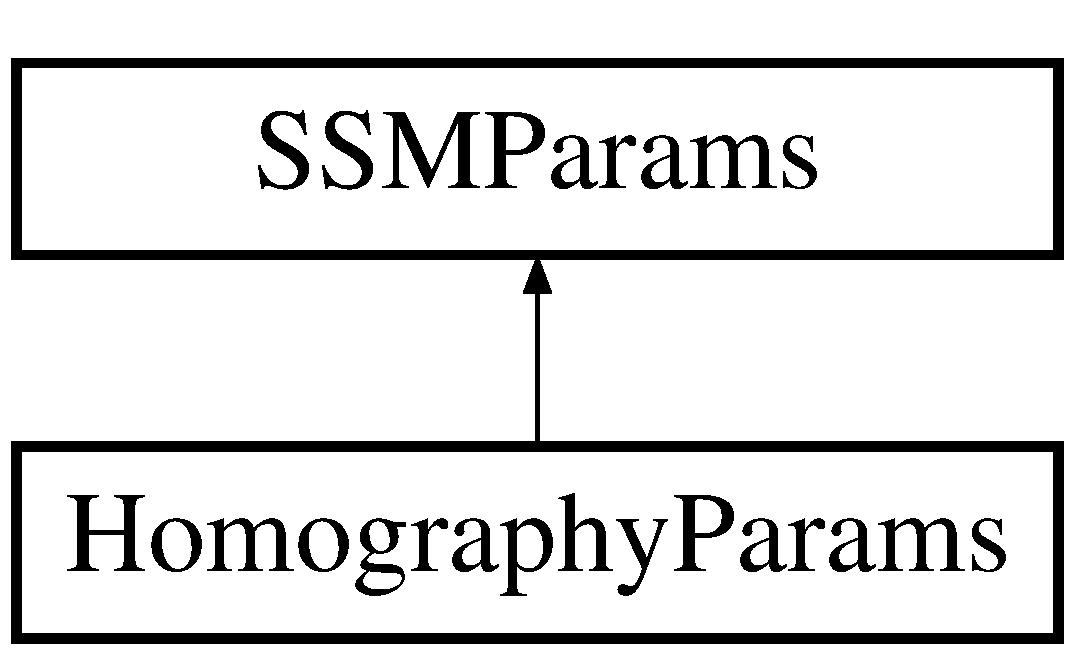
\includegraphics[height=2.000000cm]{structHomographyParams}
\end{center}
\end{figure}
\subsection*{Public Member Functions}
\begin{DoxyCompactItemize}
\item 
\hypertarget{structHomographyParams_a54b5691a136afd404b9e8d3fffb0b826}{{\bfseries Homography\-Params} (const \hyperlink{structSSMParams}{S\-S\-M\-Params} $\ast$ssm\-\_\-params, bool \-\_\-normalized\-\_\-init, bool \-\_\-corner\-\_\-based\-\_\-sampling, bool \-\_\-debug\-\_\-mode)}\label{structHomographyParams_a54b5691a136afd404b9e8d3fffb0b826}

\item 
\hypertarget{structHomographyParams_accfb40e571f90f5ca63ccd2e73e1aa66}{{\bfseries Homography\-Params} (const \hyperlink{structHomographyParams}{Homography\-Params} $\ast$params=nullptr)}\label{structHomographyParams_accfb40e571f90f5ca63ccd2e73e1aa66}

\end{DoxyCompactItemize}
\subsection*{Public Attributes}
\begin{DoxyCompactItemize}
\item 
\hypertarget{structHomographyParams_a91b89d78a80de11e7653363faee17185}{bool {\bfseries normalized\-\_\-init}}\label{structHomographyParams_a91b89d78a80de11e7653363faee17185}

\item 
\hypertarget{structHomographyParams_a27e529fdd5f4617f9508f153e2756be1}{bool {\bfseries corner\-\_\-based\-\_\-sampling}}\label{structHomographyParams_a27e529fdd5f4617f9508f153e2756be1}

\item 
\hypertarget{structHomographyParams_a5c2f4ae8537622aa5f9c12913c6f6e83}{bool {\bfseries debug\-\_\-mode}}\label{structHomographyParams_a5c2f4ae8537622aa5f9c12913c6f6e83}

\end{DoxyCompactItemize}


The documentation for this struct was generated from the following file\-:\begin{DoxyCompactItemize}
\item 
S\-S\-M/include/mtf/\-S\-S\-M/Homography.\-h\end{DoxyCompactItemize}

\hypertarget{classIALK}{\section{I\-A\-L\-K$<$ A\-M, S\-S\-M $>$ Class Template Reference}
\label{classIALK}\index{I\-A\-L\-K$<$ A\-M, S\-S\-M $>$@{I\-A\-L\-K$<$ A\-M, S\-S\-M $>$}}
}
Inheritance diagram for I\-A\-L\-K$<$ A\-M, S\-S\-M $>$\-:\begin{figure}[H]
\begin{center}
\leavevmode
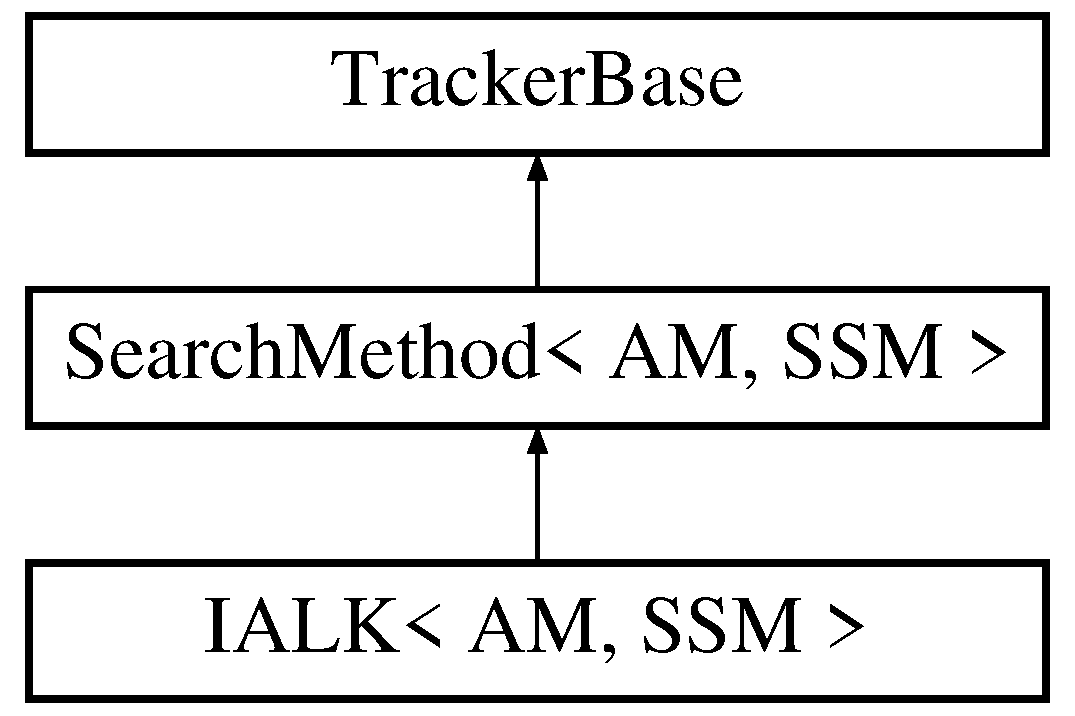
\includegraphics[height=3.000000cm]{classIALK}
\end{center}
\end{figure}
\subsection*{Public Types}
\begin{DoxyCompactItemize}
\item 
\hypertarget{classIALK_abf0584c933a8ee778a08df64eddf95cb}{typedef \hyperlink{structIALKParams}{I\-A\-L\-K\-Params} {\bfseries Param\-Type}}\label{classIALK_abf0584c933a8ee778a08df64eddf95cb}

\item 
\hypertarget{classIALK_add56895de517b7b2cd6619a384ef432a}{typedef Param\-Type\-::\-Hess\-Type {\bfseries Hess\-Type}}\label{classIALK_add56895de517b7b2cd6619a384ef432a}

\end{DoxyCompactItemize}
\subsection*{Public Member Functions}
\begin{DoxyCompactItemize}
\item 
\hypertarget{classIALK_ab051d8ec7bfdb2272c5831ea4cd66a65}{{\bfseries I\-A\-L\-K} (const \hyperlink{structIALKParams}{Param\-Type} $\ast$ialk\-\_\-params=nullptr, const \hyperlink{structAMParams}{A\-M\-Params} $\ast$am\-\_\-params=nullptr, const \hyperlink{structSSMParams}{S\-S\-M\-Params} $\ast$ssm\-\_\-params=nullptr)}\label{classIALK_ab051d8ec7bfdb2272c5831ea4cd66a65}

\item 
\hypertarget{classIALK_afa975ae63c0f6713b7af349541926d1c}{void {\bfseries initialize} (const cv\-::\-Mat \&corners) override}\label{classIALK_afa975ae63c0f6713b7af349541926d1c}

\item 
\hypertarget{classIALK_ac2bc288bb64c904ac4e7735799e60c6f}{void {\bfseries update} () override}\label{classIALK_ac2bc288bb64c904ac4e7735799e60c6f}

\end{DoxyCompactItemize}
\subsection*{Public Attributes}
\begin{DoxyCompactItemize}
\item 
\hypertarget{classIALK_a8b7e25577fed0a548f13637dbf9bb016}{\hyperlink{structIALKParams}{Param\-Type} {\bfseries params}}\label{classIALK_a8b7e25577fed0a548f13637dbf9bb016}

\end{DoxyCompactItemize}
\subsection*{Protected Attributes}
\begin{DoxyCompactItemize}
\item 
\hypertarget{classIALK_a088b47de1bfc774d06ed471f3c49e246}{Row\-Vector\-Xd \hyperlink{classIALK_a088b47de1bfc774d06ed471f3c49e246}{jacobian}}\label{classIALK_a088b47de1bfc774d06ed471f3c49e246}

\begin{DoxyCompactList}\small\item\em 1 x S Jacobian of the A\-M error norm w.\-r.\-t. S\-S\-M state vector \end{DoxyCompactList}\item 
\hypertarget{classIALK_a2a9adc8908a42e6ef3ae9a4e3bc80840}{Matrix\-Xd \hyperlink{classIALK_a2a9adc8908a42e6ef3ae9a4e3bc80840}{hessian}}\label{classIALK_a2a9adc8908a42e6ef3ae9a4e3bc80840}

\begin{DoxyCompactList}\small\item\em S x S Hessian of the A\-M error norm w.\-r.\-t. S\-S\-M state vector. \end{DoxyCompactList}\item 
Matrix\-Xd \hyperlink{classIALK_a56a3ab9d611d6f87029491b5d9da8a7d}{init\-\_\-pix\-\_\-jacobian}
\begin{DoxyCompactList}\small\item\em N x S jacobians of the pix values w.\-r.\-t the S\-S\-M state vector where N = resx $\ast$ resy is the no. \end{DoxyCompactList}\item 
\hypertarget{classIALK_a2c635c3e6b8963345921317dd0a35e73}{Matrix\-Xd {\bfseries curr\-\_\-pix\-\_\-jacobian}}\label{classIALK_a2c635c3e6b8963345921317dd0a35e73}

\item 
\hypertarget{classIALK_a6a0d1395726fca89e7146c821bcb5967}{Matrix\-Xd \hyperlink{classIALK_a6a0d1395726fca89e7146c821bcb5967}{init\-\_\-pix\-\_\-hessian}}\label{classIALK_a6a0d1395726fca89e7146c821bcb5967}

\begin{DoxyCompactList}\small\item\em N x S x S hessians of the pixel values w.\-r.\-t the S\-S\-M state vector stored as a (S$\ast$\-S) x N 2\-D matrix. \end{DoxyCompactList}\item 
\hypertarget{classIALK_a06943e47f54e36699fe80500dc0ab7d4}{Matrix\-Xd {\bfseries curr\-\_\-pix\-\_\-hessian}}\label{classIALK_a06943e47f54e36699fe80500dc0ab7d4}

\item 
\hypertarget{classIALK_a52e12fae87d02868a0f4bb0e4782e8f1}{Matrix24d {\bfseries prev\-\_\-corners}}\label{classIALK_a52e12fae87d02868a0f4bb0e4782e8f1}

\item 
\hypertarget{classIALK_a962943fb279254d91cda28296183f556}{Vector\-Xd {\bfseries ssm\-\_\-update}}\label{classIALK_a962943fb279254d91cda28296183f556}

\item 
\hypertarget{classIALK_a06bd9af1aa0ee4a3f364e4377dbf30f9}{Matrix3d {\bfseries warp\-\_\-update}}\label{classIALK_a06bd9af1aa0ee4a3f364e4377dbf30f9}

\item 
\hypertarget{classIALK_a62a8292024fd92a6edf95109c75235d0}{int {\bfseries frame\-\_\-id}}\label{classIALK_a62a8292024fd92a6edf95109c75235d0}

\end{DoxyCompactItemize}


\subsection{Member Data Documentation}
\hypertarget{classIALK_a56a3ab9d611d6f87029491b5d9da8a7d}{\index{I\-A\-L\-K@{I\-A\-L\-K}!init\-\_\-pix\-\_\-jacobian@{init\-\_\-pix\-\_\-jacobian}}
\index{init\-\_\-pix\-\_\-jacobian@{init\-\_\-pix\-\_\-jacobian}!IALK@{I\-A\-L\-K}}
\subsubsection[{init\-\_\-pix\-\_\-jacobian}]{\setlength{\rightskip}{0pt plus 5cm}template$<$class A\-M , class S\-S\-M $>$ Matrix\-Xd {\bf I\-A\-L\-K}$<$ A\-M, S\-S\-M $>$\-::init\-\_\-pix\-\_\-jacobian\hspace{0.3cm}{\ttfamily [protected]}}}\label{classIALK_a56a3ab9d611d6f87029491b5d9da8a7d}


N x S jacobians of the pix values w.\-r.\-t the S\-S\-M state vector where N = resx $\ast$ resy is the no. 

of pixels in the object patch N x S jacobians of the pix values w.\-r.\-t the S\-S\-M state vector 

The documentation for this class was generated from the following file\-:\begin{DoxyCompactItemize}
\item 
S\-M/include/mtf/\-S\-M/I\-A\-L\-K.\-h\end{DoxyCompactItemize}

\hypertarget{classIALK2}{\section{I\-A\-L\-K2$<$ A\-M, S\-S\-M $>$ Class Template Reference}
\label{classIALK2}\index{I\-A\-L\-K2$<$ A\-M, S\-S\-M $>$@{I\-A\-L\-K2$<$ A\-M, S\-S\-M $>$}}
}
Inheritance diagram for I\-A\-L\-K2$<$ A\-M, S\-S\-M $>$\-:\begin{figure}[H]
\begin{center}
\leavevmode
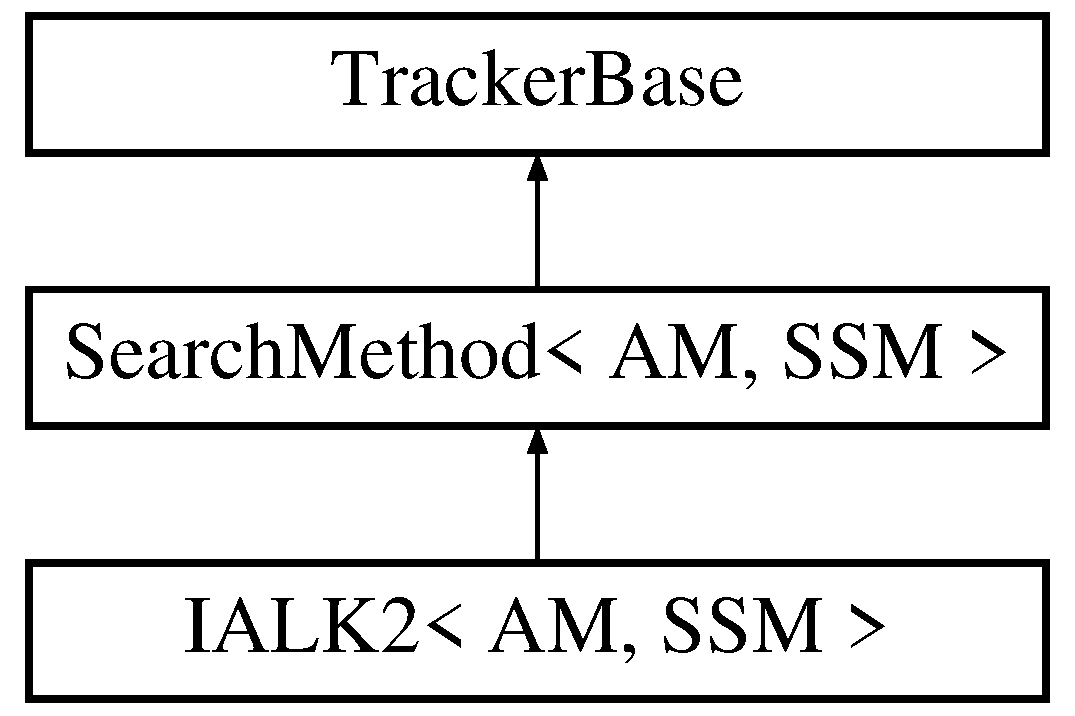
\includegraphics[height=3.000000cm]{classIALK2}
\end{center}
\end{figure}
\subsection*{Public Types}
\begin{DoxyCompactItemize}
\item 
\hypertarget{classIALK2_aaf71baa2009274abafe1f0ffc99cbb73}{typedef \hyperlink{structIALK2Params}{I\-A\-L\-K2\-Params} {\bfseries Param\-Type}}\label{classIALK2_aaf71baa2009274abafe1f0ffc99cbb73}

\item 
\hypertarget{classIALK2_a06929e07f9be24fe60291d760f6a667d}{typedef Param\-Type\-::\-Hess\-Type {\bfseries Hess\-Type}}\label{classIALK2_a06929e07f9be24fe60291d760f6a667d}

\end{DoxyCompactItemize}
\subsection*{Public Member Functions}
\begin{DoxyCompactItemize}
\item 
\hypertarget{classIALK2_a44df892466a7a49197ddc3da43a3443c}{{\bfseries I\-A\-L\-K2} (const \hyperlink{structIALK2Params}{Param\-Type} $\ast$iclk\-\_\-params=N\-U\-L\-L, const \hyperlink{structAMParams}{A\-M\-Params} $\ast$am\-\_\-params=N\-U\-L\-L, const \hyperlink{structSSMParams}{S\-S\-M\-Params} $\ast$ssm\-\_\-params=N\-U\-L\-L)}\label{classIALK2_a44df892466a7a49197ddc3da43a3443c}

\item 
\hypertarget{classIALK2_a36d6c057a850223ce0436945d837dfb6}{void {\bfseries initialize} (const cv\-::\-Mat \&corners) override}\label{classIALK2_a36d6c057a850223ce0436945d837dfb6}

\item 
\hypertarget{classIALK2_a9f9cbdb110c86602334ca6a5db31445e}{void {\bfseries update} () override}\label{classIALK2_a9f9cbdb110c86602334ca6a5db31445e}

\end{DoxyCompactItemize}
\subsection*{Public Attributes}
\begin{DoxyCompactItemize}
\item 
\hypertarget{classIALK2_af42772e069e1cb89bd849eb9b9dac21f}{\hyperlink{structIALK2Params}{Param\-Type} {\bfseries params}}\label{classIALK2_af42772e069e1cb89bd849eb9b9dac21f}

\item 
\hypertarget{classIALK2_a3b8688db64e652e1812953e6a9e103da}{Row\-Vector\-Xd \hyperlink{classIALK2_a3b8688db64e652e1812953e6a9e103da}{jacobian}}\label{classIALK2_a3b8688db64e652e1812953e6a9e103da}

\begin{DoxyCompactList}\small\item\em 1 x S Jacobian of the A\-M error norm w.\-r.\-t. S\-S\-M state vector \end{DoxyCompactList}\item 
\hypertarget{classIALK2_af0bae2ddd35a1a773f27de5bb30b64e1}{Matrix\-Xd \hyperlink{classIALK2_af0bae2ddd35a1a773f27de5bb30b64e1}{hessian}}\label{classIALK2_af0bae2ddd35a1a773f27de5bb30b64e1}

\begin{DoxyCompactList}\small\item\em S x S Hessian of the A\-M error norm w.\-r.\-t. S\-S\-M state vector. \end{DoxyCompactList}\item 
\hypertarget{classIALK2_a75785853d6458e94213451095324d061}{Matrix\-Xd \hyperlink{classIALK2_a75785853d6458e94213451095324d061}{init\-\_\-pix\-\_\-jacobian}}\label{classIALK2_a75785853d6458e94213451095324d061}

\begin{DoxyCompactList}\small\item\em N x S jacobians of the pixel values w.\-r.\-t the S\-S\-M state vector. \end{DoxyCompactList}\item 
\hypertarget{classIALK2_ab6507033c73d5f4c53103389772f0bf7}{Matrix\-Xd {\bfseries curr\-\_\-pix\-\_\-jacobian}}\label{classIALK2_ab6507033c73d5f4c53103389772f0bf7}

\item 
\hypertarget{classIALK2_a5eac5510857a25408c1e903b4f4f36ac}{Matrix\-Xd \hyperlink{classIALK2_a5eac5510857a25408c1e903b4f4f36ac}{init\-\_\-pix\-\_\-hessian}}\label{classIALK2_a5eac5510857a25408c1e903b4f4f36ac}

\begin{DoxyCompactList}\small\item\em N x S x S hessians of the pixel values w.\-r.\-t the S\-S\-M state vector stored as a (S$\ast$\-S) x N 2\-D matrix. \end{DoxyCompactList}\item 
\hypertarget{classIALK2_a7af6e78521d67b691653423a18e77a0b}{Matrix\-Xd {\bfseries curr\-\_\-pix\-\_\-hessian}}\label{classIALK2_a7af6e78521d67b691653423a18e77a0b}

\item 
\hypertarget{classIALK2_a8f3465edc4b825c9e2b897f24f1ad156}{Matrix24d {\bfseries prev\-\_\-corners}}\label{classIALK2_a8f3465edc4b825c9e2b897f24f1ad156}

\item 
\hypertarget{classIALK2_ac4b58e3e8002bd51b7287d7da40aed6c}{Vector\-Xd {\bfseries ssm\-\_\-update}}\label{classIALK2_ac4b58e3e8002bd51b7287d7da40aed6c}

\item 
\hypertarget{classIALK2_abb1bc228c541af9ff0acaca60f0dfd85}{Vector\-Xd {\bfseries inv\-\_\-update}}\label{classIALK2_abb1bc228c541af9ff0acaca60f0dfd85}

\item 
\hypertarget{classIALK2_a0afdaf9be67063c26648f9e2312c988b}{int {\bfseries frame\-\_\-id}}\label{classIALK2_a0afdaf9be67063c26648f9e2312c988b}

\end{DoxyCompactItemize}
\subsection*{Additional Inherited Members}


The documentation for this class was generated from the following file\-:\begin{DoxyCompactItemize}
\item 
S\-M/include/mtf/\-S\-M/I\-A\-L\-K2.\-h\end{DoxyCompactItemize}

\hypertarget{structIALK2Params}{\section{I\-A\-L\-K2\-Params Struct Reference}
\label{structIALK2Params}\index{I\-A\-L\-K2\-Params@{I\-A\-L\-K2\-Params}}
}
\subsection*{Public Types}
\begin{DoxyCompactItemize}
\item 
enum {\bfseries Hess\-Type} \{ {\bfseries Initial\-Self}, 
{\bfseries Current\-Self}, 
{\bfseries Std}
 \}
\end{DoxyCompactItemize}
\subsection*{Public Member Functions}
\begin{DoxyCompactItemize}
\item 
\hyperlink{structIALK2Params_aa4414dc3fa55e3a72441f0cd6cff6385}{I\-A\-L\-K2\-Params} (int \-\_\-max\-\_\-iters, double \-\_\-epsilon, Hess\-Type \-\_\-hess\-\_\-type, bool \-\_\-sec\-\_\-ord\-\_\-hess, bool \-\_\-debug\-\_\-mode)
\begin{DoxyCompactList}\small\item\em decides whether logging data will be printed for debugging purposes; \end{DoxyCompactList}\item 
\hypertarget{structIALK2Params_aead4476bbe6cff177f438fbaad1de8c8}{{\bfseries I\-A\-L\-K2\-Params} (\hyperlink{structIALK2Params}{I\-A\-L\-K2\-Params} $\ast$params=nullptr)}\label{structIALK2Params_aead4476bbe6cff177f438fbaad1de8c8}

\end{DoxyCompactItemize}
\subsection*{Public Attributes}
\begin{DoxyCompactItemize}
\item 
\hypertarget{structIALK2Params_a233a0a1db5ab529f2a07f6f67160b2d4}{int {\bfseries max\-\_\-iters}}\label{structIALK2Params_a233a0a1db5ab529f2a07f6f67160b2d4}

\item 
\hypertarget{structIALK2Params_a58a3a704ad4c91ca93e451c4974ed481}{double \hyperlink{structIALK2Params_a58a3a704ad4c91ca93e451c4974ed481}{epsilon}}\label{structIALK2Params_a58a3a704ad4c91ca93e451c4974ed481}

\begin{DoxyCompactList}\small\item\em maximum iterations of the \hyperlink{classIALK2}{I\-A\-L\-K2} algorithm to run for each frame \end{DoxyCompactList}\item 
\hypertarget{structIALK2Params_a0b26ec58400a3188e7b220f64b9304b1}{Hess\-Type \hyperlink{structIALK2Params_a0b26ec58400a3188e7b220f64b9304b1}{hess\-\_\-type}}\label{structIALK2Params_a0b26ec58400a3188e7b220f64b9304b1}

\begin{DoxyCompactList}\small\item\em maximum L1 norm of the state update vector at which to stop the iterations \end{DoxyCompactList}\item 
\hypertarget{structIALK2Params_a399fce526b085fe80ee5c718e8b49123}{bool {\bfseries sec\-\_\-ord\-\_\-hess}}\label{structIALK2Params_a399fce526b085fe80ee5c718e8b49123}

\item 
\hypertarget{structIALK2Params_a2f8c3a4e1587a122a19ef6876d6cb1eb}{bool {\bfseries debug\-\_\-mode}}\label{structIALK2Params_a2f8c3a4e1587a122a19ef6876d6cb1eb}

\end{DoxyCompactItemize}


\subsection{Constructor \& Destructor Documentation}
\hypertarget{structIALK2Params_aa4414dc3fa55e3a72441f0cd6cff6385}{\index{I\-A\-L\-K2\-Params@{I\-A\-L\-K2\-Params}!I\-A\-L\-K2\-Params@{I\-A\-L\-K2\-Params}}
\index{I\-A\-L\-K2\-Params@{I\-A\-L\-K2\-Params}!IALK2Params@{I\-A\-L\-K2\-Params}}
\subsubsection[{I\-A\-L\-K2\-Params}]{\setlength{\rightskip}{0pt plus 5cm}I\-A\-L\-K2\-Params\-::\-I\-A\-L\-K2\-Params (
\begin{DoxyParamCaption}
\item[{int}]{\-\_\-max\-\_\-iters, }
\item[{double}]{\-\_\-epsilon, }
\item[{Hess\-Type}]{\-\_\-hess\-\_\-type, }
\item[{bool}]{\-\_\-sec\-\_\-ord\-\_\-hess, }
\item[{bool}]{\-\_\-debug\-\_\-mode}
\end{DoxyParamCaption}
)\hspace{0.3cm}{\ttfamily [inline]}}}\label{structIALK2Params_aa4414dc3fa55e3a72441f0cd6cff6385}


decides whether logging data will be printed for debugging purposes; 

only matters if logging is enabled at compile time 

The documentation for this struct was generated from the following file\-:\begin{DoxyCompactItemize}
\item 
S\-M/include/mtf/\-S\-M/I\-A\-L\-K2.\-h\end{DoxyCompactItemize}

\hypertarget{structIALKParams}{\section{I\-A\-L\-K\-Params Struct Reference}
\label{structIALKParams}\index{I\-A\-L\-K\-Params@{I\-A\-L\-K\-Params}}
}
\subsection*{Public Types}
\begin{DoxyCompactItemize}
\item 
enum {\bfseries Hess\-Type} \{ {\bfseries Initial\-Self}, 
{\bfseries Current\-Self}, 
{\bfseries Std}
 \}
\end{DoxyCompactItemize}
\subsection*{Public Member Functions}
\begin{DoxyCompactItemize}
\item 
\hyperlink{structIALKParams_a355ce721a1366121d3762bf82e7dd3b2}{I\-A\-L\-K\-Params} (int \-\_\-max\-\_\-iters, double \-\_\-epsilon, Hess\-Type \-\_\-hess\-\_\-type, bool \-\_\-sec\-\_\-ord\-\_\-hess, bool \-\_\-debug\-\_\-mode)
\begin{DoxyCompactList}\small\item\em decides whether logging data will be printed for debugging purposes; \end{DoxyCompactList}\item 
\hypertarget{structIALKParams_abc5c24da3c94dd247a4ef36252c9c590}{{\bfseries I\-A\-L\-K\-Params} (const \hyperlink{structIALKParams}{I\-A\-L\-K\-Params} $\ast$params=nullptr)}\label{structIALKParams_abc5c24da3c94dd247a4ef36252c9c590}

\end{DoxyCompactItemize}
\subsection*{Public Attributes}
\begin{DoxyCompactItemize}
\item 
\hypertarget{structIALKParams_abbc8d072e4003a2b2d860517efe7f4a0}{int {\bfseries max\-\_\-iters}}\label{structIALKParams_abbc8d072e4003a2b2d860517efe7f4a0}

\item 
\hypertarget{structIALKParams_ac88ea122543c062702a53294b2933266}{double \hyperlink{structIALKParams_ac88ea122543c062702a53294b2933266}{epsilon}}\label{structIALKParams_ac88ea122543c062702a53294b2933266}

\begin{DoxyCompactList}\small\item\em maximum iterations of the \hyperlink{classIALK}{I\-A\-L\-K} algorithm to run for each frame \end{DoxyCompactList}\item 
\hypertarget{structIALKParams_a11111c7058984020a1b89ac473da8fb8}{Hess\-Type \hyperlink{structIALKParams_a11111c7058984020a1b89ac473da8fb8}{hess\-\_\-type}}\label{structIALKParams_a11111c7058984020a1b89ac473da8fb8}

\begin{DoxyCompactList}\small\item\em maximum L1 norm of the state update vector at which to stop the iterations \end{DoxyCompactList}\item 
\hypertarget{structIALKParams_a9cec9fe2c7f76a5be66b6b19f02daed9}{bool {\bfseries sec\-\_\-ord\-\_\-hess}}\label{structIALKParams_a9cec9fe2c7f76a5be66b6b19f02daed9}

\item 
\hypertarget{structIALKParams_a745a6ab9e74acdf4c36f9c39a022f603}{bool {\bfseries debug\-\_\-mode}}\label{structIALKParams_a745a6ab9e74acdf4c36f9c39a022f603}

\end{DoxyCompactItemize}


\subsection{Constructor \& Destructor Documentation}
\hypertarget{structIALKParams_a355ce721a1366121d3762bf82e7dd3b2}{\index{I\-A\-L\-K\-Params@{I\-A\-L\-K\-Params}!I\-A\-L\-K\-Params@{I\-A\-L\-K\-Params}}
\index{I\-A\-L\-K\-Params@{I\-A\-L\-K\-Params}!IALKParams@{I\-A\-L\-K\-Params}}
\subsubsection[{I\-A\-L\-K\-Params}]{\setlength{\rightskip}{0pt plus 5cm}I\-A\-L\-K\-Params\-::\-I\-A\-L\-K\-Params (
\begin{DoxyParamCaption}
\item[{int}]{\-\_\-max\-\_\-iters, }
\item[{double}]{\-\_\-epsilon, }
\item[{Hess\-Type}]{\-\_\-hess\-\_\-type, }
\item[{bool}]{\-\_\-sec\-\_\-ord\-\_\-hess, }
\item[{bool}]{\-\_\-debug\-\_\-mode}
\end{DoxyParamCaption}
)}}\label{structIALKParams_a355ce721a1366121d3762bf82e7dd3b2}


decides whether logging data will be printed for debugging purposes; 

only matters if logging is enabled at compile time 

The documentation for this struct was generated from the following file\-:\begin{DoxyCompactItemize}
\item 
S\-M/include/mtf/\-S\-M/I\-A\-L\-K\-Params.\-h\end{DoxyCompactItemize}

\hypertarget{classICLK}{\section{I\-C\-L\-K$<$ A\-M, S\-S\-M $>$ Class Template Reference}
\label{classICLK}\index{I\-C\-L\-K$<$ A\-M, S\-S\-M $>$@{I\-C\-L\-K$<$ A\-M, S\-S\-M $>$}}
}
Inheritance diagram for I\-C\-L\-K$<$ A\-M, S\-S\-M $>$\-:\begin{figure}[H]
\begin{center}
\leavevmode
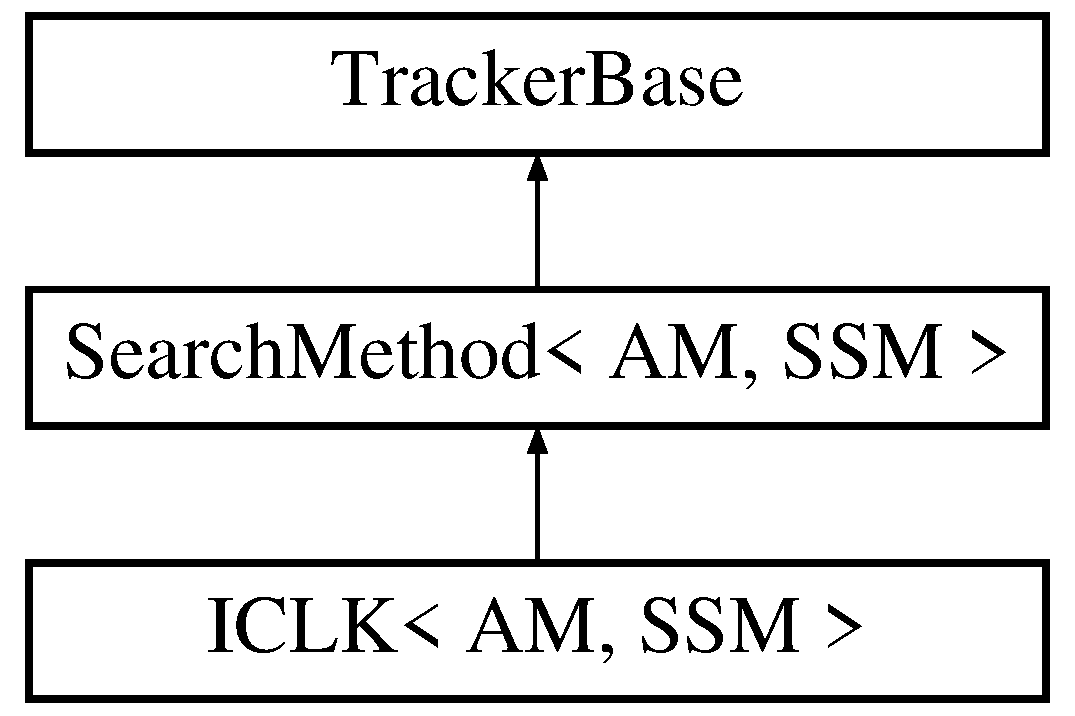
\includegraphics[height=3.000000cm]{classICLK}
\end{center}
\end{figure}
\subsection*{Public Types}
\begin{DoxyCompactItemize}
\item 
\hypertarget{classICLK_ac9497f5d15d1f31253f4426e2a3f7117}{typedef \hyperlink{structICLKParams}{I\-C\-L\-K\-Params} {\bfseries Param\-Type}}\label{classICLK_ac9497f5d15d1f31253f4426e2a3f7117}

\item 
\hypertarget{classICLK_aa06240a7f337a177e44b2c0a31740bcc}{typedef Param\-Type\-::\-Hess\-Type {\bfseries Hess\-Type}}\label{classICLK_aa06240a7f337a177e44b2c0a31740bcc}

\end{DoxyCompactItemize}
\subsection*{Public Member Functions}
\begin{DoxyCompactItemize}
\item 
\hypertarget{classICLK_af0a58581126b936bc65d4d0ae83bf8f4}{{\bfseries I\-C\-L\-K} (const \hyperlink{structICLKParams}{Param\-Type} $\ast$iclk\-\_\-params=nullptr, const \hyperlink{structAMParams}{A\-M\-Params} $\ast$am\-\_\-params=nullptr, const \hyperlink{structSSMParams}{S\-S\-M\-Params} $\ast$ssm\-\_\-params=nullptr)}\label{classICLK_af0a58581126b936bc65d4d0ae83bf8f4}

\item 
\hypertarget{classICLK_a2850eda56cffa035f8dc624473bcbd40}{void {\bfseries initialize} (const cv\-::\-Mat \&corners) override}\label{classICLK_a2850eda56cffa035f8dc624473bcbd40}

\item 
\hypertarget{classICLK_ac53506808de6a0eb3859427c18445735}{void {\bfseries update} () override}\label{classICLK_ac53506808de6a0eb3859427c18445735}

\item 
\hypertarget{classICLK_a7fe543f27a9d6a2400208c8aadcb760f}{void {\bfseries set\-Region} (const cv\-::\-Mat \&corners) override}\label{classICLK_a7fe543f27a9d6a2400208c8aadcb760f}

\end{DoxyCompactItemize}
\subsection*{Public Attributes}
\begin{DoxyCompactItemize}
\item 
\hypertarget{classICLK_a2945308452b028417df86764bcf8a831}{\hyperlink{structICLKParams}{Param\-Type} {\bfseries params}}\label{classICLK_a2945308452b028417df86764bcf8a831}

\item 
\hypertarget{classICLK_afbabfa8946549910cc4e643788dc81e7}{Row\-Vector\-Xd \hyperlink{classICLK_afbabfa8946549910cc4e643788dc81e7}{jacobian}}\label{classICLK_afbabfa8946549910cc4e643788dc81e7}

\begin{DoxyCompactList}\small\item\em 1 x S Jacobian of the A\-M error norm w.\-r.\-t. S\-S\-M state vector \end{DoxyCompactList}\item 
\hypertarget{classICLK_ad13c158447f2aeec0dc13198294fd071}{Matrix\-Xd \hyperlink{classICLK_ad13c158447f2aeec0dc13198294fd071}{hessian}}\label{classICLK_ad13c158447f2aeec0dc13198294fd071}

\begin{DoxyCompactList}\small\item\em S x S Hessian of the A\-M error norm w.\-r.\-t. S\-S\-M state vector. \end{DoxyCompactList}\item 
\hypertarget{classICLK_ae35df2f2b1aacb31f06cbd236924fa10}{Matrix\-Xd \hyperlink{classICLK_ae35df2f2b1aacb31f06cbd236924fa10}{init\-\_\-pix\-\_\-jacobian}}\label{classICLK_ae35df2f2b1aacb31f06cbd236924fa10}

\begin{DoxyCompactList}\small\item\em N x S jacobians of the pixel values w.\-r.\-t the S\-S\-M state vector. \end{DoxyCompactList}\item 
\hypertarget{classICLK_aa534a53a187fcb3e7aa47327502c93bf}{Matrix\-Xd {\bfseries curr\-\_\-pix\-\_\-jacobian}}\label{classICLK_aa534a53a187fcb3e7aa47327502c93bf}

\item 
\hypertarget{classICLK_a1cef372827b58727ad0f1977974a9877}{Matrix\-Xd \hyperlink{classICLK_a1cef372827b58727ad0f1977974a9877}{init\-\_\-pix\-\_\-hessian}}\label{classICLK_a1cef372827b58727ad0f1977974a9877}

\begin{DoxyCompactList}\small\item\em N x S x S hessians of the pixel values w.\-r.\-t the S\-S\-M state vector stored as a (S$\ast$\-S) x N 2\-D matrix. \end{DoxyCompactList}\item 
\hypertarget{classICLK_acf2fed0787c9f2128a6ecdaa6a39866c}{Matrix\-Xd {\bfseries curr\-\_\-pix\-\_\-hessian}}\label{classICLK_acf2fed0787c9f2128a6ecdaa6a39866c}

\item 
\hypertarget{classICLK_a1abdd3bba3f87338dba1bc225fd33229}{Matrix24d {\bfseries prev\-\_\-corners}}\label{classICLK_a1abdd3bba3f87338dba1bc225fd33229}

\item 
\hypertarget{classICLK_a6cda93b3ed854937a169a619a4949958}{Vector\-Xd {\bfseries ssm\-\_\-update}}\label{classICLK_a6cda93b3ed854937a169a619a4949958}

\item 
\hypertarget{classICLK_a85a1b1c824bc5af2f2ccda32d7d9f5b6}{Vector\-Xd {\bfseries inv\-\_\-update}}\label{classICLK_a85a1b1c824bc5af2f2ccda32d7d9f5b6}

\item 
\hypertarget{classICLK_a309c08fe9ddf14a34480382d276cda32}{int {\bfseries frame\-\_\-id}}\label{classICLK_a309c08fe9ddf14a34480382d276cda32}

\end{DoxyCompactItemize}
\subsection*{Additional Inherited Members}


The documentation for this class was generated from the following file\-:\begin{DoxyCompactItemize}
\item 
S\-M/include/mtf/\-S\-M/I\-C\-L\-K.\-h\end{DoxyCompactItemize}

\hypertarget{structICLKParams}{\section{I\-C\-L\-K\-Params Struct Reference}
\label{structICLKParams}\index{I\-C\-L\-K\-Params@{I\-C\-L\-K\-Params}}
}
\subsection*{Public Types}
\begin{DoxyCompactItemize}
\item 
enum {\bfseries Hess\-Type} \{ {\bfseries Initial\-Self}, 
{\bfseries Current\-Self}, 
{\bfseries Std}
 \}
\end{DoxyCompactItemize}
\subsection*{Public Member Functions}
\begin{DoxyCompactItemize}
\item 
\hyperlink{structICLKParams_a2af0cd6dfd77ac0fb5ecf4e50485a970}{I\-C\-L\-K\-Params} (int \-\_\-max\-\_\-iters, double \-\_\-epsilon, Hess\-Type \-\_\-hess\-\_\-type, bool \-\_\-sec\-\_\-ord\-\_\-hess, bool \-\_\-update\-\_\-ssm, bool \-\_\-chained\-\_\-warp, bool \-\_\-debug\-\_\-mode)
\begin{DoxyCompactList}\small\item\em decides whether logging data will be printed for debugging purposes; \end{DoxyCompactList}\item 
\hypertarget{structICLKParams_a9a13691f0aaf8d10e4700e77ddeb6270}{{\bfseries I\-C\-L\-K\-Params} (const \hyperlink{structICLKParams}{I\-C\-L\-K\-Params} $\ast$params=nullptr)}\label{structICLKParams_a9a13691f0aaf8d10e4700e77ddeb6270}

\end{DoxyCompactItemize}
\subsection*{Static Public Member Functions}
\begin{DoxyCompactItemize}
\item 
\hypertarget{structICLKParams_af84dd9fd7cbcdf2219943d35a80b4005}{static const char $\ast$ {\bfseries to\-String} (Hess\-Type \hyperlink{structICLKParams_a07bb2297e80debb470a3696e1e1877c6}{hess\-\_\-type})}\label{structICLKParams_af84dd9fd7cbcdf2219943d35a80b4005}

\end{DoxyCompactItemize}
\subsection*{Public Attributes}
\begin{DoxyCompactItemize}
\item 
\hypertarget{structICLKParams_a61c0bc94051ecefae6ffd263ec5bb6e0}{int {\bfseries max\-\_\-iters}}\label{structICLKParams_a61c0bc94051ecefae6ffd263ec5bb6e0}

\item 
\hypertarget{structICLKParams_a4390c0932e546ff1f947af5d0b24b162}{double \hyperlink{structICLKParams_a4390c0932e546ff1f947af5d0b24b162}{epsilon}}\label{structICLKParams_a4390c0932e546ff1f947af5d0b24b162}

\begin{DoxyCompactList}\small\item\em maximum iterations of the \hyperlink{classICLK}{I\-C\-L\-K} algorithm to run for each frame \end{DoxyCompactList}\item 
\hypertarget{structICLKParams_a07bb2297e80debb470a3696e1e1877c6}{Hess\-Type \hyperlink{structICLKParams_a07bb2297e80debb470a3696e1e1877c6}{hess\-\_\-type}}\label{structICLKParams_a07bb2297e80debb470a3696e1e1877c6}

\begin{DoxyCompactList}\small\item\em maximum L2 norm of the state update vector at which to stop the iterations \end{DoxyCompactList}\item 
\hypertarget{structICLKParams_aae7c66e6a6d77b2a3a95891064ec3cf2}{bool {\bfseries sec\-\_\-ord\-\_\-hess}}\label{structICLKParams_aae7c66e6a6d77b2a3a95891064ec3cf2}

\item 
\hypertarget{structICLKParams_a8e6e92fada7da215608de2913d77c1bf}{bool {\bfseries update\-\_\-ssm}}\label{structICLKParams_a8e6e92fada7da215608de2913d77c1bf}

\item 
\hypertarget{structICLKParams_a69537756ab955142e5f1a6302e6449a6}{bool {\bfseries chained\-\_\-warp}}\label{structICLKParams_a69537756ab955142e5f1a6302e6449a6}

\item 
\hypertarget{structICLKParams_a09054b8d4a1aac5060ddf2850ec989be}{bool {\bfseries debug\-\_\-mode}}\label{structICLKParams_a09054b8d4a1aac5060ddf2850ec989be}

\end{DoxyCompactItemize}


\subsection{Constructor \& Destructor Documentation}
\hypertarget{structICLKParams_a2af0cd6dfd77ac0fb5ecf4e50485a970}{\index{I\-C\-L\-K\-Params@{I\-C\-L\-K\-Params}!I\-C\-L\-K\-Params@{I\-C\-L\-K\-Params}}
\index{I\-C\-L\-K\-Params@{I\-C\-L\-K\-Params}!ICLKParams@{I\-C\-L\-K\-Params}}
\subsubsection[{I\-C\-L\-K\-Params}]{\setlength{\rightskip}{0pt plus 5cm}I\-C\-L\-K\-Params\-::\-I\-C\-L\-K\-Params (
\begin{DoxyParamCaption}
\item[{int}]{\-\_\-max\-\_\-iters, }
\item[{double}]{\-\_\-epsilon, }
\item[{Hess\-Type}]{\-\_\-hess\-\_\-type, }
\item[{bool}]{\-\_\-sec\-\_\-ord\-\_\-hess, }
\item[{bool}]{\-\_\-update\-\_\-ssm, }
\item[{bool}]{\-\_\-chained\-\_\-warp, }
\item[{bool}]{\-\_\-debug\-\_\-mode}
\end{DoxyParamCaption}
)}}\label{structICLKParams_a2af0cd6dfd77ac0fb5ecf4e50485a970}


decides whether logging data will be printed for debugging purposes; 

only matters if logging is enabled at compile time 

The documentation for this struct was generated from the following file\-:\begin{DoxyCompactItemize}
\item 
S\-M/include/mtf/\-S\-M/I\-C\-L\-K\-Params.\-h\end{DoxyCompactItemize}

\hypertarget{classIlluminationModel}{\section{Illumination\-Model Class Reference}
\label{classIlluminationModel}\index{Illumination\-Model@{Illumination\-Model}}
}


Illumination Model is a parametric function that transforms pixel values extracted from a patch to account for illumination changes g(\-I, a)\-: R(\-N) x R(\-K) -\/$>$ R(\-N)  




{\ttfamily \#include $<$Illumination\-Model.\-h$>$}

Inheritance diagram for Illumination\-Model\-:\begin{figure}[H]
\begin{center}
\leavevmode
\includegraphics[height=2.000000cm]{classIlluminationModel}
\end{center}
\end{figure}
\subsection*{Public Types}
\begin{DoxyCompactItemize}
\item 
enum {\bfseries Pix\-Hess\-Type} \{ {\bfseries Constant}, 
{\bfseries Diagonal}, 
{\bfseries General}
 \}
\end{DoxyCompactItemize}
\subsection*{Public Member Functions}
\begin{DoxyCompactItemize}
\item 
\hypertarget{classIlluminationModel_a15002b87b3e5d8028ec2a41e4b449858}{{\bfseries Illumination\-Model} (const \hyperlink{structILMParams}{I\-L\-M\-Params} $\ast$ilm\-\_\-params)}\label{classIlluminationModel_a15002b87b3e5d8028ec2a41e4b449858}

\item 
\hypertarget{classIlluminationModel_aa0cd6e5f5ae8a3ec40a236850ba9f4c6}{virtual int {\bfseries get\-State\-Size} () const =0}\label{classIlluminationModel_aa0cd6e5f5ae8a3ec40a236850ba9f4c6}

\item 
\hypertarget{classIlluminationModel_a7659625f49e862d79e805d52b6f25000}{virtual void {\bfseries initialize} (double $\ast$p)}\label{classIlluminationModel_a7659625f49e862d79e805d52b6f25000}

\item 
\hypertarget{classIlluminationModel_ae059487d9714a6318276354d814a9f7e}{virtual void {\bfseries apply} (double $\ast$g, const double $\ast$I, const double $\ast$p)=0}\label{classIlluminationModel_ae059487d9714a6318276354d814a9f7e}

\item 
\hypertarget{classIlluminationModel_a3e55966b7f58f87be86b687664f6b692}{virtual void {\bfseries invert} (double $\ast$inv\-\_\-p, const double $\ast$p)=0}\label{classIlluminationModel_a3e55966b7f58f87be86b687664f6b692}

\item 
\hypertarget{classIlluminationModel_a6552e22adee7a0ce77c9d8c5855719ea}{virtual void {\bfseries update} (double $\ast$new\-\_\-p, const double $\ast$old\-\_\-p, const double $\ast$dp)=0}\label{classIlluminationModel_a6552e22adee7a0ce77c9d8c5855719ea}

\item 
\hypertarget{classIlluminationModel_a451142f32d7de0618032004bb601b75b}{virtual void {\bfseries cmpt\-Param\-Jacobian} (double $\ast$df\-\_\-dp, const double $\ast$df\-\_\-dg, const double $\ast$I, const double $\ast$p)=0}\label{classIlluminationModel_a451142f32d7de0618032004bb601b75b}

\item 
\hypertarget{classIlluminationModel_ae35b55b3cde313c4366a9d97423335ad}{virtual void {\bfseries cmpt\-Pix\-Jacobian} (double $\ast$df\-\_\-d\-I, const double $\ast$df\-\_\-dg, const double $\ast$I, const double $\ast$p)=0}\label{classIlluminationModel_ae35b55b3cde313c4366a9d97423335ad}

\item 
\hypertarget{classIlluminationModel_a77c82e70e4bb6364e1e18b8e22ad5d1c}{virtual void {\bfseries cmpt\-Param\-Hessian} (double $\ast$d2f\-\_\-dp2, const double $\ast$d2f\-\_\-dg2, const double $\ast$df\-\_\-dg, const double $\ast$I, const double $\ast$p)=0}\label{classIlluminationModel_a77c82e70e4bb6364e1e18b8e22ad5d1c}

\item 
\hypertarget{classIlluminationModel_a8451e6a9da72a6c0d12ff2656cc18917}{virtual void {\bfseries cmpt\-Pix\-Hessian} (double $\ast$d2f\-\_\-d\-I2, const double $\ast$d2f\-\_\-dg2, const double $\ast$df\-\_\-dg, const double $\ast$I, const double $\ast$p)=0}\label{classIlluminationModel_a8451e6a9da72a6c0d12ff2656cc18917}

\item 
\hypertarget{classIlluminationModel_a6c6906805e0e9f740dba0db5c3d5d510}{virtual void {\bfseries cmpt\-Cross\-Hessian} (double $\ast$d2f\-\_\-dp\-\_\-d\-I, const double $\ast$d2f\-\_\-dg2, const double $\ast$df\-\_\-dg, const double $\ast$I, const double $\ast$p)=0}\label{classIlluminationModel_a6c6906805e0e9f740dba0db5c3d5d510}

\item 
\hypertarget{classIlluminationModel_a3607504c6f586e340329d9c612621d1e}{virtual void {\bfseries set\-Pix\-Hess\-Type} (Pix\-Hess\-Type \-\_\-d2f\-\_\-dg2\-\_\-type)}\label{classIlluminationModel_a3607504c6f586e340329d9c612621d1e}

\item 
\hypertarget{classIlluminationModel_ae83c96af1e730acbd58b8aac73766e78}{virtual Pix\-Hess\-Type {\bfseries get\-Pix\-Hess\-Type} ()=0}\label{classIlluminationModel_ae83c96af1e730acbd58b8aac73766e78}

\end{DoxyCompactItemize}
\subsection*{Public Attributes}
\begin{DoxyCompactItemize}
\item 
\hypertarget{classIlluminationModel_ad96e45e4f447219d90eac2e1fe0f7848}{string {\bfseries name}}\label{classIlluminationModel_ad96e45e4f447219d90eac2e1fe0f7848}

\item 
\hypertarget{classIlluminationModel_ab1f442b134340b3061937f0dad5d3e83}{bool {\bfseries apply\-\_\-on\-\_\-init}}\label{classIlluminationModel_ab1f442b134340b3061937f0dad5d3e83}

\end{DoxyCompactItemize}
\subsection*{Protected Attributes}
\begin{DoxyCompactItemize}
\item 
\hypertarget{classIlluminationModel_aff37102b88464457214ecf5675aa13e0}{int {\bfseries resx}}\label{classIlluminationModel_aff37102b88464457214ecf5675aa13e0}

\item 
\hypertarget{classIlluminationModel_a769764d8cb182650f4b91db9c7c83e9d}{int {\bfseries resy}}\label{classIlluminationModel_a769764d8cb182650f4b91db9c7c83e9d}

\item 
\hypertarget{classIlluminationModel_ae9b8983f2e6a518492c6b254a35884fa}{int {\bfseries n\-\_\-pix}}\label{classIlluminationModel_ae9b8983f2e6a518492c6b254a35884fa}

\item 
\hypertarget{classIlluminationModel_ae6a5f2a2373262dbcd413aedf4ed3701}{Pix\-Hess\-Type {\bfseries d2f\-\_\-dg2\-\_\-type}}\label{classIlluminationModel_ae6a5f2a2373262dbcd413aedf4ed3701}

\end{DoxyCompactItemize}


\subsection{Detailed Description}
Illumination Model is a parametric function that transforms pixel values extracted from a patch to account for illumination changes g(\-I, a)\-: R(\-N) x R(\-K) -\/$>$ R(\-N) 

The documentation for this class was generated from the following file\-:\begin{DoxyCompactItemize}
\item 
A\-M/include/mtf/\-A\-M/Illumination\-Model.\-h\end{DoxyCompactItemize}

\hypertarget{structILMParams}{\section{I\-L\-M\-Params Struct Reference}
\label{structILMParams}\index{I\-L\-M\-Params@{I\-L\-M\-Params}}
}
Inheritance diagram for I\-L\-M\-Params\-:\begin{figure}[H]
\begin{center}
\leavevmode
\includegraphics[height=2.000000cm]{structILMParams}
\end{center}
\end{figure}
\subsection*{Public Member Functions}
\begin{DoxyCompactItemize}
\item 
\hypertarget{structILMParams_abc1c67bd1a99c21afa1269ee8871febd}{{\bfseries I\-L\-M\-Params} (int \-\_\-resx, int \-\_\-resy)}\label{structILMParams_abc1c67bd1a99c21afa1269ee8871febd}

\item 
\hypertarget{structILMParams_a4b99a98e0f116eed7abd67c960db6a72}{{\bfseries I\-L\-M\-Params} (const \hyperlink{structILMParams}{I\-L\-M\-Params} $\ast$ilm\-\_\-params=nullptr)}\label{structILMParams_a4b99a98e0f116eed7abd67c960db6a72}

\end{DoxyCompactItemize}
\subsection*{Public Attributes}
\begin{DoxyCompactItemize}
\item 
\hypertarget{structILMParams_a3be05b5483b99b430dc6442bc22e95d3}{int \hyperlink{structILMParams_a3be05b5483b99b430dc6442bc22e95d3}{resx}}\label{structILMParams_a3be05b5483b99b430dc6442bc22e95d3}

\begin{DoxyCompactList}\small\item\em horizontal and vertical sampling resolutions \end{DoxyCompactList}\item 
\hypertarget{structILMParams_a21b4270e30846afbd17cd2b730f927da}{int {\bfseries resy}}\label{structILMParams_a21b4270e30846afbd17cd2b730f927da}

\end{DoxyCompactItemize}


The documentation for this struct was generated from the following file\-:\begin{DoxyCompactItemize}
\item 
A\-M/include/mtf/\-A\-M/Illumination\-Model.\-h\end{DoxyCompactItemize}

\hypertarget{classImageBase}{\section{Image\-Base Class Reference}
\label{classImageBase}\index{Image\-Base@{Image\-Base}}
}
Inheritance diagram for Image\-Base\-:\begin{figure}[H]
\begin{center}
\leavevmode
\includegraphics[height=12.000000cm]{classImageBase}
\end{center}
\end{figure}
\subsection*{Public Types}
\begin{DoxyCompactItemize}
\item 
\hypertarget{classImageBase_aa0f54a34c4ce87f5b72c7c741145a94e}{typedef Eig\-Img\-T \hyperlink{classImageBase_aa0f54a34c4ce87f5b72c7c741145a94e}{Image\-T}}\label{classImageBase_aa0f54a34c4ce87f5b72c7c741145a94e}

\begin{DoxyCompactList}\small\item\em convenience type if grayscale image is used as input by the A\-M \end{DoxyCompactList}\end{DoxyCompactItemize}
\subsection*{Public Member Functions}
\begin{DoxyCompactItemize}
\item 
\hypertarget{classImageBase_a44574be90999ffd0c7a9d700608005db}{{\bfseries Image\-Base} (const \hyperlink{structImgParams}{Img\-Params} $\ast$img\-\_\-params=nullptr, const int \-\_\-n\-\_\-channels=1)}\label{classImageBase_a44574be90999ffd0c7a9d700608005db}

\item 
\hypertarget{classImageBase_afc86a63579a95bf7ee05aff4c1f21522}{virtual int \hyperlink{classImageBase_afc86a63579a95bf7ee05aff4c1f21522}{input\-Type} () const }\label{classImageBase_afc86a63579a95bf7ee05aff4c1f21522}

\begin{DoxyCompactList}\small\item\em return the type of Open\-C\-V Mat image the A\-M requires as input; typically either C\-V\-\_\-32\-F\-C3 or C\-V\-\_\-32\-F\-C1 \end{DoxyCompactList}\item 
virtual const cv\-::\-Mat \& \hyperlink{classImageBase_aeab7b6efa7fa9c98bec6e20594113bf0}{get\-Curr\-Img} () const 
\begin{DoxyCompactList}\small\item\em accessor methods; these are not defined as 'const' since an appearance model may like to make some last moment changes to the variable being accessed before returning it to can avoid any unnecessary computations concerning the variable (e.\-g. \end{DoxyCompactList}\item 
\hypertarget{classImageBase_aa28aca0398cdecce95ad382665363938}{virtual int {\bfseries get\-Img\-Height} () const }\label{classImageBase_aa28aca0398cdecce95ad382665363938}

\item 
\hypertarget{classImageBase_a250f19163c9fe65ba2a4f137ce2bf90b}{virtual int {\bfseries get\-Img\-Width} () const }\label{classImageBase_a250f19163c9fe65ba2a4f137ce2bf90b}

\item 
\hypertarget{classImageBase_afe923eb9b81d60f333e2dfe0131bdd20}{virtual int {\bfseries get\-Res\-X} () const }\label{classImageBase_afe923eb9b81d60f333e2dfe0131bdd20}

\item 
\hypertarget{classImageBase_a2017f3faf5fe85d6cc26e471041c45ee}{virtual int {\bfseries get\-Res\-Y} () const }\label{classImageBase_a2017f3faf5fe85d6cc26e471041c45ee}

\item 
\hypertarget{classImageBase_a2151ca10c29dfe674c5503cd1f7352c6}{virtual int {\bfseries get\-N\-Pix} () const }\label{classImageBase_a2151ca10c29dfe674c5503cd1f7352c6}

\item 
\hypertarget{classImageBase_a5d28f1bd86db90f9d1a056545828f444}{virtual int {\bfseries get\-N\-Channels} () const }\label{classImageBase_a5d28f1bd86db90f9d1a056545828f444}

\item 
\hypertarget{classImageBase_a3e4aac727c581d0a2745641669864df1}{virtual int {\bfseries get\-Patch\-Size} () const }\label{classImageBase_a3e4aac727c581d0a2745641669864df1}

\item 
\hypertarget{classImageBase_a152c661dd701949ab326dfff6caf5fba}{virtual double {\bfseries get\-Grad\-Offset} () const }\label{classImageBase_a152c661dd701949ab326dfff6caf5fba}

\item 
\hypertarget{classImageBase_a23a89704145102741c43eaeef9dba171}{virtual double {\bfseries get\-Hess\-Offset} () const }\label{classImageBase_a23a89704145102741c43eaeef9dba171}

\item 
\hypertarget{classImageBase_a6f7d67dad333f72a55f49c4aa63ef1c0}{virtual const Pix\-Val\-T \& {\bfseries get\-Init\-Pix\-Vals} () const }\label{classImageBase_a6f7d67dad333f72a55f49c4aa63ef1c0}

\item 
\hypertarget{classImageBase_a99a58357f0eaa15c70e9c0ee21da9d05}{virtual const Pix\-Grad\-T \& {\bfseries get\-Init\-Pix\-Grad} () const }\label{classImageBase_a99a58357f0eaa15c70e9c0ee21da9d05}

\item 
\hypertarget{classImageBase_a2b0e6211578a63205e936412dfee1fb6}{virtual const Pix\-Hess\-T \& {\bfseries get\-Init\-Pix\-Hess} () const }\label{classImageBase_a2b0e6211578a63205e936412dfee1fb6}

\item 
\hypertarget{classImageBase_a28ec6b021eb2cbb57386979cbb8dd8f1}{virtual const Pix\-Val\-T \& {\bfseries get\-Curr\-Pix\-Vals} () const }\label{classImageBase_a28ec6b021eb2cbb57386979cbb8dd8f1}

\item 
\hypertarget{classImageBase_a5626c50674100fc7acd0364029ae2827}{virtual const Pix\-Grad\-T \& {\bfseries get\-Curr\-Pix\-Grad} () const }\label{classImageBase_a5626c50674100fc7acd0364029ae2827}

\item 
\hypertarget{classImageBase_a7793589a55eff60418443f6dca953f05}{virtual const Pix\-Hess\-T \& {\bfseries get\-Curr\-Pix\-Hess} () const }\label{classImageBase_a7793589a55eff60418443f6dca953f05}

\item 
\hypertarget{classImageBase_a9eb8fba660685c2a74b2cf2658b103ed}{virtual void \hyperlink{classImageBase_a9eb8fba660685c2a74b2cf2658b103ed}{set\-Curr\-Img} (const cv\-::\-Mat \&cv\-\_\-img)}\label{classImageBase_a9eb8fba660685c2a74b2cf2658b103ed}

\begin{DoxyCompactList}\small\item\em modifier methods; \end{DoxyCompactList}\item 
\hypertarget{classImageBase_a8d50bae23e438e75a51cc6d38a0cb933}{virtual void {\bfseries set\-Init\-Pix\-Vals} (const Pix\-Val\-T \&pix\-\_\-vals)}\label{classImageBase_a8d50bae23e438e75a51cc6d38a0cb933}

\item 
\hypertarget{classImageBase_aadecea7cb19c93e5b0558f219344c599}{virtual void {\bfseries set\-Init\-Pix\-Grad} (const Pix\-Grad\-T \&pix\-\_\-grad)}\label{classImageBase_aadecea7cb19c93e5b0558f219344c599}

\item 
\hypertarget{classImageBase_a0c74c497e73154bfc99c3fe3790b138c}{virtual void {\bfseries set\-Init\-Pix\-Hess} (const Pix\-Hess\-T \&pix\-\_\-hess)}\label{classImageBase_a0c74c497e73154bfc99c3fe3790b138c}

\item 
\hypertarget{classImageBase_a63fe6a4acb201ee9418a96e28dbabc14}{virtual void {\bfseries set\-Curr\-Pix\-Vals} (const Pix\-Val\-T \&pix\-\_\-vals)}\label{classImageBase_a63fe6a4acb201ee9418a96e28dbabc14}

\item 
\hypertarget{classImageBase_a0f8d3b81eca127f6094b2804d2155905}{virtual void {\bfseries set\-Curr\-Pix\-Grad} (const Pix\-Grad\-T \&pix\-\_\-grad)}\label{classImageBase_a0f8d3b81eca127f6094b2804d2155905}

\item 
\hypertarget{classImageBase_a123a6ed44636823f12e9b49abdd80c99}{virtual void {\bfseries set\-Curr\-Pix\-Hess} (const Pix\-Hess\-T \&pix\-\_\-hess)}\label{classImageBase_a123a6ed44636823f12e9b49abdd80c99}

\item 
\hypertarget{classImageBase_ab803d031b7ed046b00e69d691504e14e}{virtual void \hyperlink{classImageBase_ab803d031b7ed046b00e69d691504e14e}{initialize\-Pix\-Vals} (const Pts\-T \&init\-\_\-pts)}\label{classImageBase_ab803d031b7ed046b00e69d691504e14e}

\begin{DoxyCompactList}\small\item\em initialization methods -\/ to be called once when the tracker is initialized \end{DoxyCompactList}\item 
virtual void \hyperlink{classImageBase_a2aeec772d5c4de56f4e8fbfd4f08e69d}{initialize\-Pix\-Grad} (const Grad\-Pts\-T \&warped\-\_\-offset\-\_\-pts)
\begin{DoxyCompactList}\small\item\em functions to compute image differentials (gradient and hessian) are overloaded since there are two ways to define them\-: \end{DoxyCompactList}\item 
virtual void \hyperlink{classImageBase_aa81f72f3d41e1be570b162789b8221d6}{initialize\-Pix\-Grad} (const Pts\-T \&init\-\_\-pts)
\item 
virtual void \hyperlink{classImageBase_a9e8f70830c1caffda808830f1cdf939d}{initialize\-Pix\-Hess} (const Pts\-T \&init\-\_\-pts, const Hess\-Pts\-T \&warped\-\_\-offset\-\_\-pts)
\item 
virtual void \hyperlink{classImageBase_a8ab724371b3b3874a026e530b40c4082}{initialize\-Pix\-Hess} (const Pts\-T \&init\-\_\-pts)
\item 
\hypertarget{classImageBase_a807fb84431ec6a39338a3809cd2f02bc}{virtual void {\bfseries update\-Pix\-Vals} (const Pts\-T \&curr\-\_\-pts)}\label{classImageBase_a807fb84431ec6a39338a3809cd2f02bc}

\item 
\hypertarget{classImageBase_af5d79c319b0feb05b1670289ff4c8f57}{virtual void {\bfseries update\-Pix\-Grad} (const Grad\-Pts\-T \&warped\-\_\-offset\-\_\-pts)}\label{classImageBase_af5d79c319b0feb05b1670289ff4c8f57}

\item 
\hypertarget{classImageBase_aec28bd13871be3cbfa37da46ce589f0c}{virtual void {\bfseries update\-Pix\-Grad} (const Pts\-T \&curr\-\_\-pts)}\label{classImageBase_aec28bd13871be3cbfa37da46ce589f0c}

\item 
\hypertarget{classImageBase_aaac5ac3287b29d744e6dd847e879e862}{virtual void {\bfseries update\-Pix\-Hess} (const Pts\-T \&curr\-\_\-pts)}\label{classImageBase_aaac5ac3287b29d744e6dd847e879e862}

\item 
\hypertarget{classImageBase_a155b46226f9824af99c7628ad7c33228}{virtual void {\bfseries update\-Pix\-Hess} (const Pts\-T \&curr\-\_\-pts, const Hess\-Pts\-T \&warped\-\_\-offset\-\_\-pts)}\label{classImageBase_a155b46226f9824af99c7628ad7c33228}

\item 
\hypertarget{classImageBase_ab356e9ea42029bdf2e527e517da9f524}{virtual void \hyperlink{classImageBase_ab356e9ea42029bdf2e527e517da9f524}{update\-Template} (const Pts\-T \&curr\-\_\-pts)}\label{classImageBase_ab356e9ea42029bdf2e527e517da9f524}

\begin{DoxyCompactList}\small\item\em optional function to incorporate online learning or adaptation of the object template being tracked this should be called with the final location of the object (obtained by the search process) in the curent image by default it updates the template with the running average of all the object patches seen so far \end{DoxyCompactList}\item 
\hypertarget{classImageBase_a296af969f6f7b03c850007076397a026}{virtual void \hyperlink{classImageBase_a296af969f6f7b03c850007076397a026}{extract\-Patch} (Vector\-Xd \&pix\-\_\-vals, const Pts\-T \&curr\-\_\-pts)}\label{classImageBase_a296af969f6f7b03c850007076397a026}

\begin{DoxyCompactList}\small\item\em general utility function to extract raw pixel values from the current image at the specified points; might be useful for visualization purposes as the curr\-\_\-pix\-\_\-vals might not have raw pixel values; \end{DoxyCompactList}\item 
\hypertarget{classImageBase_ae8f0d73deaf9ddd78ba37120b164e5b0}{virtual \hyperlink{structImgStatus}{Img\-Status} $\ast$ {\bfseries is\-Initialized} ()=0}\label{classImageBase_ae8f0d73deaf9ddd78ba37120b164e5b0}

\end{DoxyCompactItemize}
\subsection*{Protected Attributes}
\begin{DoxyCompactItemize}
\item 
\hypertarget{classImageBase_a05bb3e22989361a082501f48286f58ce}{Eig\-Img\-T \hyperlink{classImageBase_a05bb3e22989361a082501f48286f58ce}{curr\-\_\-img}}\label{classImageBase_a05bb3e22989361a082501f48286f58ce}

\begin{DoxyCompactList}\small\item\em Eigen structure shaing memory with the Open\-C\-V image used by default with grayscale inputs. \end{DoxyCompactList}\item 
\hypertarget{classImageBase_a79c1a5f750185761ce3467f9eac640fe}{cv\-::\-Mat \hyperlink{classImageBase_a79c1a5f750185761ce3467f9eac640fe}{curr\-\_\-img\-\_\-cv}}\label{classImageBase_a79c1a5f750185761ce3467f9eac640fe}

\begin{DoxyCompactList}\small\item\em Open\-C\-V image used by default with multi channel inputs. \end{DoxyCompactList}\item 
\hypertarget{classImageBase_a51a4b10eff8f050199c4b69225111ad9}{int \hyperlink{classImageBase_a51a4b10eff8f050199c4b69225111ad9}{img\-\_\-height}}\label{classImageBase_a51a4b10eff8f050199c4b69225111ad9}

\begin{DoxyCompactList}\small\item\em height and width of the input images \end{DoxyCompactList}\item 
\hypertarget{classImageBase_a02e207fa46966b86c63618fbfe0192e0}{int {\bfseries img\-\_\-width}}\label{classImageBase_a02e207fa46966b86c63618fbfe0192e0}

\item 
\hypertarget{classImageBase_a4ea85cd1ec4b0655d0de1d452eb0e1ec}{int \hyperlink{classImageBase_a4ea85cd1ec4b0655d0de1d452eb0e1ec}{resx}}\label{classImageBase_a4ea85cd1ec4b0655d0de1d452eb0e1ec}

\begin{DoxyCompactList}\small\item\em horizontal and vertical sampling resolutions for the object patch \end{DoxyCompactList}\item 
\hypertarget{classImageBase_adb1512179414cadfbca54e58de914320}{int {\bfseries resy}}\label{classImageBase_adb1512179414cadfbca54e58de914320}

\item 
\hypertarget{classImageBase_a01bbe6e54a59a6a54885222225233040}{int \hyperlink{classImageBase_a01bbe6e54a59a6a54885222225233040}{n\-\_\-pix}}\label{classImageBase_a01bbe6e54a59a6a54885222225233040}

\begin{DoxyCompactList}\small\item\em no. of pixels in the sampled image patch to be tracked \end{DoxyCompactList}\item 
const int \hyperlink{classImageBase_ac16eaa560cdf51fc9232ae115c3567e2}{n\-\_\-channels}
\begin{DoxyCompactList}\small\item\em no. \end{DoxyCompactList}\item 
\hypertarget{classImageBase_a71d9ec399436e3c833ad7323670f1ed5}{int \hyperlink{classImageBase_a71d9ec399436e3c833ad7323670f1ed5}{patch\-\_\-size}}\label{classImageBase_a71d9ec399436e3c833ad7323670f1ed5}

\begin{DoxyCompactList}\small\item\em size of the vector that represents the object patch in the image, typically n\-\_\-pix$\ast$n\-\_\-channels \end{DoxyCompactList}\item 
Pix\-Val\-T \hyperlink{classImageBase_a6e5beaedb0a6d8e511446443dc2b80dc}{I0}
\begin{DoxyCompactList}\small\item\em let N = n\-\_\-pix = no. of pixels and C = n\-\_\-channels = no. of channels \end{DoxyCompactList}\item 
\hypertarget{classImageBase_ab681301644f53a0609a53214c93aede0}{Pix\-Val\-T {\bfseries It}}\label{classImageBase_ab681301644f53a0609a53214c93aede0}

\item 
Pix\-Grad\-T \hyperlink{classImageBase_a932c969a6b33c3d3d4e2c120fa8fd815}{d\-I0\-\_\-dx}
\begin{DoxyCompactList}\small\item\em (N$\ast$\-C) x 2 jacobian of pixel values in the warped image w.\-r.\-t. \end{DoxyCompactList}\item 
\hypertarget{classImageBase_a5b86e56c04d2bdfc846764e6ab5c52ee}{Pix\-Grad\-T {\bfseries d\-It\-\_\-dx}}\label{classImageBase_a5b86e56c04d2bdfc846764e6ab5c52ee}

\item 
Pix\-Hess\-T \hyperlink{classImageBase_a4540fc64d3c65262b2c489d9380f09d3}{d2\-I0\-\_\-dx2}
\begin{DoxyCompactList}\small\item\em 4 x (N$\ast$\-C) Hessian of pixel values in the warped image w.\-r.\-t. \end{DoxyCompactList}\item 
\hypertarget{classImageBase_a242904300650df81767929bfd312998b}{Pix\-Hess\-T {\bfseries d2\-It\-\_\-dx2}}\label{classImageBase_a242904300650df81767929bfd312998b}

\item 
\hypertarget{classImageBase_ab4c84af6cf0169cae8497bb1666fbd47}{double \hyperlink{classImageBase_ab4c84af6cf0169cae8497bb1666fbd47}{pix\-\_\-norm\-\_\-add}}\label{classImageBase_ab4c84af6cf0169cae8497bb1666fbd47}

\begin{DoxyCompactList}\small\item\em additive and multiplicative factors for normalizing pixel values \end{DoxyCompactList}\item 
\hypertarget{classImageBase_a35b4b321a878a44c3ee71a528689e091}{double {\bfseries pix\-\_\-norm\-\_\-mult}}\label{classImageBase_a35b4b321a878a44c3ee71a528689e091}

\item 
\hypertarget{classImageBase_a7dd1820d273ccb2e48ce0d0e2003d0b3}{int \hyperlink{classImageBase_a7dd1820d273ccb2e48ce0d0e2003d0b3}{frame\-\_\-count}}\label{classImageBase_a7dd1820d273ccb2e48ce0d0e2003d0b3}

\begin{DoxyCompactList}\small\item\em incremented once during initialization and thereafter everytime the template is updated \end{DoxyCompactList}\item 
\hypertarget{classImageBase_a3d7c35acde3316f70cc71a09f843f811}{double \hyperlink{classImageBase_a3d7c35acde3316f70cc71a09f843f811}{grad\-\_\-eps}}\label{classImageBase_a3d7c35acde3316f70cc71a09f843f811}

\begin{DoxyCompactList}\small\item\em offsets to use for computing the numerical image gradient and hessian \end{DoxyCompactList}\item 
\hypertarget{classImageBase_a7248011def174fd4c80414796927991b}{double {\bfseries hess\-\_\-eps}}\label{classImageBase_a7248011def174fd4c80414796927991b}

\end{DoxyCompactItemize}


\subsection{Member Function Documentation}
\hypertarget{classImageBase_aeab7b6efa7fa9c98bec6e20594113bf0}{\index{Image\-Base@{Image\-Base}!get\-Curr\-Img@{get\-Curr\-Img}}
\index{get\-Curr\-Img@{get\-Curr\-Img}!ImageBase@{Image\-Base}}
\subsubsection[{get\-Curr\-Img}]{\setlength{\rightskip}{0pt plus 5cm}virtual const cv\-::\-Mat\& Image\-Base\-::get\-Curr\-Img (
\begin{DoxyParamCaption}
{}
\end{DoxyParamCaption}
) const\hspace{0.3cm}{\ttfamily [inline]}, {\ttfamily [virtual]}}}\label{classImageBase_aeab7b6efa7fa9c98bec6e20594113bf0}


accessor methods; these are not defined as 'const' since an appearance model may like to make some last moment changes to the variable being accessed before returning it to can avoid any unnecessary computations concerning the variable (e.\-g. 

in its 'update' function) unless it is actually accessed; \hypertarget{classImageBase_a2aeec772d5c4de56f4e8fbfd4f08e69d}{\index{Image\-Base@{Image\-Base}!initialize\-Pix\-Grad@{initialize\-Pix\-Grad}}
\index{initialize\-Pix\-Grad@{initialize\-Pix\-Grad}!ImageBase@{Image\-Base}}
\subsubsection[{initialize\-Pix\-Grad}]{\setlength{\rightskip}{0pt plus 5cm}virtual void Image\-Base\-::initialize\-Pix\-Grad (
\begin{DoxyParamCaption}
\item[{const Grad\-Pts\-T \&}]{warped\-\_\-offset\-\_\-pts}
\end{DoxyParamCaption}
)\hspace{0.3cm}{\ttfamily [virtual]}}}\label{classImageBase_a2aeec772d5c4de56f4e8fbfd4f08e69d}


functions to compute image differentials (gradient and hessian) are overloaded since there are two ways to define them\-: 


\begin{DoxyEnumerate}
\item differential of the warped image\-: the image is warped first, then its differential is computed at the base (unwarped) locations
\item warp of the image differential\-: differential is computed in the image coordinates and evaluated at the given (presumably warped) locations
\end{DoxyEnumerate}
\begin{DoxyEnumerate}
\item gradient of the warped image 
\end{DoxyEnumerate}

Reimplemented in \hyperlink{classSCV_ad72451578ca3a16031924fcd238ae066}{S\-C\-V}, and \hyperlink{classSumOfAMs_ad58a98f4c992ef4ea3971ef34108a0de}{Sum\-Of\-A\-Ms}.

\hypertarget{classImageBase_aa81f72f3d41e1be570b162789b8221d6}{\index{Image\-Base@{Image\-Base}!initialize\-Pix\-Grad@{initialize\-Pix\-Grad}}
\index{initialize\-Pix\-Grad@{initialize\-Pix\-Grad}!ImageBase@{Image\-Base}}
\subsubsection[{initialize\-Pix\-Grad}]{\setlength{\rightskip}{0pt plus 5cm}virtual void Image\-Base\-::initialize\-Pix\-Grad (
\begin{DoxyParamCaption}
\item[{const Pts\-T \&}]{init\-\_\-pts}
\end{DoxyParamCaption}
)\hspace{0.3cm}{\ttfamily [virtual]}}}\label{classImageBase_aa81f72f3d41e1be570b162789b8221d6}

\begin{DoxyEnumerate}
\item warp of the image gradient 
\end{DoxyEnumerate}

Reimplemented in \hyperlink{classSCV_acb828cbac2799da234dcefaf48190e7c}{S\-C\-V}, and \hyperlink{classSumOfAMs_a5471a78347467e2de3c53a9107b0ffd1}{Sum\-Of\-A\-Ms}.

\hypertarget{classImageBase_a9e8f70830c1caffda808830f1cdf939d}{\index{Image\-Base@{Image\-Base}!initialize\-Pix\-Hess@{initialize\-Pix\-Hess}}
\index{initialize\-Pix\-Hess@{initialize\-Pix\-Hess}!ImageBase@{Image\-Base}}
\subsubsection[{initialize\-Pix\-Hess}]{\setlength{\rightskip}{0pt plus 5cm}virtual void Image\-Base\-::initialize\-Pix\-Hess (
\begin{DoxyParamCaption}
\item[{const Pts\-T \&}]{init\-\_\-pts, }
\item[{const Hess\-Pts\-T \&}]{warped\-\_\-offset\-\_\-pts}
\end{DoxyParamCaption}
)\hspace{0.3cm}{\ttfamily [virtual]}}}\label{classImageBase_a9e8f70830c1caffda808830f1cdf939d}

\begin{DoxyEnumerate}
\item hessian of the warped image 
\end{DoxyEnumerate}

Reimplemented in \hyperlink{classSumOfAMs_a0d4f0a8a998165f8b37eed1984dcc700}{Sum\-Of\-A\-Ms}.

\hypertarget{classImageBase_a8ab724371b3b3874a026e530b40c4082}{\index{Image\-Base@{Image\-Base}!initialize\-Pix\-Hess@{initialize\-Pix\-Hess}}
\index{initialize\-Pix\-Hess@{initialize\-Pix\-Hess}!ImageBase@{Image\-Base}}
\subsubsection[{initialize\-Pix\-Hess}]{\setlength{\rightskip}{0pt plus 5cm}virtual void Image\-Base\-::initialize\-Pix\-Hess (
\begin{DoxyParamCaption}
\item[{const Pts\-T \&}]{init\-\_\-pts}
\end{DoxyParamCaption}
)\hspace{0.3cm}{\ttfamily [virtual]}}}\label{classImageBase_a8ab724371b3b3874a026e530b40c4082}

\begin{DoxyEnumerate}
\item warp of the image hessian 
\end{DoxyEnumerate}

Reimplemented in \hyperlink{classSumOfAMs_aae252eb6ade3ab8efbfd0d12da76e1c3}{Sum\-Of\-A\-Ms}.



\subsection{Member Data Documentation}
\hypertarget{classImageBase_a4540fc64d3c65262b2c489d9380f09d3}{\index{Image\-Base@{Image\-Base}!d2\-I0\-\_\-dx2@{d2\-I0\-\_\-dx2}}
\index{d2\-I0\-\_\-dx2@{d2\-I0\-\_\-dx2}!ImageBase@{Image\-Base}}
\subsubsection[{d2\-I0\-\_\-dx2}]{\setlength{\rightskip}{0pt plus 5cm}Pix\-Hess\-T Image\-Base\-::d2\-I0\-\_\-dx2\hspace{0.3cm}{\ttfamily [protected]}}}\label{classImageBase_a4540fc64d3c65262b2c489d9380f09d3}


4 x (N$\ast$\-C) Hessian of pixel values in the warped image w.\-r.\-t. 

pixel coordinate locations; each column of this matrix contains the 2x2 hessian for the respective location (for each channel) flasttened in the column major order; \hypertarget{classImageBase_a932c969a6b33c3d3d4e2c120fa8fd815}{\index{Image\-Base@{Image\-Base}!d\-I0\-\_\-dx@{d\-I0\-\_\-dx}}
\index{d\-I0\-\_\-dx@{d\-I0\-\_\-dx}!ImageBase@{Image\-Base}}
\subsubsection[{d\-I0\-\_\-dx}]{\setlength{\rightskip}{0pt plus 5cm}Pix\-Grad\-T Image\-Base\-::d\-I0\-\_\-dx\hspace{0.3cm}{\ttfamily [protected]}}}\label{classImageBase_a932c969a6b33c3d3d4e2c120fa8fd815}


(N$\ast$\-C) x 2 jacobian of pixel values in the warped image w.\-r.\-t. 

pixel coordinate locations aka gradient of the warped image or warp of the gradient image depending on the search method \hypertarget{classImageBase_a6e5beaedb0a6d8e511446443dc2b80dc}{\index{Image\-Base@{Image\-Base}!I0@{I0}}
\index{I0@{I0}!ImageBase@{Image\-Base}}
\subsubsection[{I0}]{\setlength{\rightskip}{0pt plus 5cm}Pix\-Val\-T Image\-Base\-::\-I0\hspace{0.3cm}{\ttfamily [protected]}}}\label{classImageBase_a6e5beaedb0a6d8e511446443dc2b80dc}


let N = n\-\_\-pix = no. of pixels and C = n\-\_\-channels = no. of channels 

pixel values for all channels in the object patch being tracked (flattened as a vector) \hypertarget{classImageBase_ac16eaa560cdf51fc9232ae115c3567e2}{\index{Image\-Base@{Image\-Base}!n\-\_\-channels@{n\-\_\-channels}}
\index{n\-\_\-channels@{n\-\_\-channels}!ImageBase@{Image\-Base}}
\subsubsection[{n\-\_\-channels}]{\setlength{\rightskip}{0pt plus 5cm}const int Image\-Base\-::n\-\_\-channels\hspace{0.3cm}{\ttfamily [protected]}}}\label{classImageBase_ac16eaa560cdf51fc9232ae115c3567e2}


no. 

of values that represent each pixel in the sampled patch defined as a constant to enable compile time optimizations 

The documentation for this class was generated from the following file\-:\begin{DoxyCompactItemize}
\item 
A\-M/include/mtf/\-A\-M/Image\-Base.\-h\end{DoxyCompactItemize}

\hypertarget{structImgParams}{\section{Img\-Params Struct Reference}
\label{structImgParams}\index{Img\-Params@{Img\-Params}}
}
Inheritance diagram for Img\-Params\-:\begin{figure}[H]
\begin{center}
\leavevmode
\includegraphics[height=12.000000cm]{structImgParams}
\end{center}
\end{figure}
\subsection*{Public Member Functions}
\begin{DoxyCompactItemize}
\item 
\hypertarget{structImgParams_a49c741a4b827149c83af1512dc04e4a9}{{\bfseries Img\-Params} (int \-\_\-resx, int \-\_\-resy, double \-\_\-grad\-\_\-eps=G\-R\-A\-D\-\_\-\-E\-P\-S, double \-\_\-hess\-\_\-eps=H\-E\-S\-S\-\_\-\-E\-P\-S)}\label{structImgParams_a49c741a4b827149c83af1512dc04e4a9}

\item 
\hypertarget{structImgParams_a68e627bc2215ae75efce0043d012f215}{{\bfseries Img\-Params} (const \hyperlink{structImgParams}{Img\-Params} $\ast$img\-\_\-params=nullptr)}\label{structImgParams_a68e627bc2215ae75efce0043d012f215}

\end{DoxyCompactItemize}
\subsection*{Public Attributes}
\begin{DoxyCompactItemize}
\item 
\hypertarget{structImgParams_aa12bf4a79cb15c878b37e424b52683c3}{int \hyperlink{structImgParams_aa12bf4a79cb15c878b37e424b52683c3}{resx}}\label{structImgParams_aa12bf4a79cb15c878b37e424b52683c3}

\begin{DoxyCompactList}\small\item\em horizontal and vertical sampling resolutions \end{DoxyCompactList}\item 
\hypertarget{structImgParams_a14ba5c6220070dfef8f12a0ec4fe14f5}{int {\bfseries resy}}\label{structImgParams_a14ba5c6220070dfef8f12a0ec4fe14f5}

\item 
\hypertarget{structImgParams_a2b802e547e383df054bd8060023a6e66}{double \hyperlink{structImgParams_a2b802e547e383df054bd8060023a6e66}{grad\-\_\-eps}}\label{structImgParams_a2b802e547e383df054bd8060023a6e66}

\begin{DoxyCompactList}\small\item\em numerical increment/decrement used for computing image hessian and gradient using the method of finite differences \end{DoxyCompactList}\item 
\hypertarget{structImgParams_af0c157dec6f1c2f4143ff1067b50274d}{double {\bfseries hess\-\_\-eps}}\label{structImgParams_af0c157dec6f1c2f4143ff1067b50274d}

\end{DoxyCompactItemize}


The documentation for this struct was generated from the following file\-:\begin{DoxyCompactItemize}
\item 
A\-M/include/mtf/\-A\-M/Image\-Base.\-h\end{DoxyCompactItemize}

\hypertarget{structImgStatus}{\section{Img\-Status Struct Reference}
\label{structImgStatus}\index{Img\-Status@{Img\-Status}}
}
Inheritance diagram for Img\-Status\-:\begin{figure}[H]
\begin{center}
\leavevmode
\includegraphics[height=2.000000cm]{structImgStatus}
\end{center}
\end{figure}
\subsection*{Public Member Functions}
\begin{DoxyCompactItemize}
\item 
\hypertarget{structImgStatus_a613cf6ca781d5bf8ffbc429bf7e56ec3}{void {\bfseries set\-Pix\-State} ()}\label{structImgStatus_a613cf6ca781d5bf8ffbc429bf7e56ec3}

\item 
\hypertarget{structImgStatus_adf986a18f22cd34178ac097ab2cb32e2}{void {\bfseries clear\-Pix\-State} ()}\label{structImgStatus_adf986a18f22cd34178ac097ab2cb32e2}

\end{DoxyCompactItemize}
\subsection*{Public Attributes}
\begin{DoxyCompactItemize}
\item 
\hypertarget{structImgStatus_a82dadcad1833463681aa1b3613f317a6}{bool {\bfseries pix\-\_\-vals}}\label{structImgStatus_a82dadcad1833463681aa1b3613f317a6}

\item 
\hypertarget{structImgStatus_a19bdab5df0acba90aee60d8bf7f48896}{bool {\bfseries pix\-\_\-grad}}\label{structImgStatus_a19bdab5df0acba90aee60d8bf7f48896}

\item 
\hypertarget{structImgStatus_a5ad02dd50c054d6a72c5a3010858cbde}{bool {\bfseries pix\-\_\-hess}}\label{structImgStatus_a5ad02dd50c054d6a72c5a3010858cbde}

\end{DoxyCompactItemize}


The documentation for this struct was generated from the following file\-:\begin{DoxyCompactItemize}
\item 
A\-M/include/mtf/\-A\-M/Image\-Base.\-h\end{DoxyCompactItemize}

\hypertarget{structgnn_1_1IndxDist}{\section{gnn\-:\-:Indx\-Dist Struct Reference}
\label{structgnn_1_1IndxDist}\index{gnn\-::\-Indx\-Dist@{gnn\-::\-Indx\-Dist}}
}
\subsection*{Public Attributes}
\begin{DoxyCompactItemize}
\item 
\hypertarget{structgnn_1_1IndxDist_a0aeaf1be2302feafacfb3edee6c748bb}{double {\bfseries dist}}\label{structgnn_1_1IndxDist_a0aeaf1be2302feafacfb3edee6c748bb}

\item 
\hypertarget{structgnn_1_1IndxDist_a301ec58399bc72b31e0882d6881f8abb}{int {\bfseries idx}}\label{structgnn_1_1IndxDist_a301ec58399bc72b31e0882d6881f8abb}

\end{DoxyCompactItemize}


The documentation for this struct was generated from the following file\-:\begin{DoxyCompactItemize}
\item 
S\-M/include/mtf/\-S\-M/G\-N\-N.\-h\end{DoxyCompactItemize}

\hypertarget{classutils_1_1InvalidTrackerState}{\section{utils\-:\-:Invalid\-Tracker\-State Class Reference}
\label{classutils_1_1InvalidTrackerState}\index{utils\-::\-Invalid\-Tracker\-State@{utils\-::\-Invalid\-Tracker\-State}}
}
Inheritance diagram for utils\-:\-:Invalid\-Tracker\-State\-:\begin{figure}[H]
\begin{center}
\leavevmode
\includegraphics[height=2.000000cm]{classutils_1_1InvalidTrackerState}
\end{center}
\end{figure}
\subsection*{Public Member Functions}
\begin{DoxyCompactItemize}
\item 
\hypertarget{classutils_1_1InvalidTrackerState_a7a989895e03cb323118511619dc40ea5}{{\bfseries Invalid\-Tracker\-State} (const char $\ast$error=\char`\"{}Invalid Tracker State found\char`\"{})}\label{classutils_1_1InvalidTrackerState_a7a989895e03cb323118511619dc40ea5}

\item 
\hypertarget{classutils_1_1InvalidTrackerState_a23242aaa03868ef958416ac9223b8fd0}{{\bfseries Invalid\-Tracker\-State} (const std\-::string error=\char`\"{}Invalid Tracker State found\char`\"{})}\label{classutils_1_1InvalidTrackerState_a23242aaa03868ef958416ac9223b8fd0}

\end{DoxyCompactItemize}


The documentation for this class was generated from the following file\-:\begin{DoxyCompactItemize}
\item 
Utilities/include/mtf/\-Utilities/excp\-Utils.\-h\end{DoxyCompactItemize}

\hypertarget{classIsometry}{\section{Isometry Class Reference}
\label{classIsometry}\index{Isometry@{Isometry}}
}
Inheritance diagram for Isometry\-:\begin{figure}[H]
\begin{center}
\leavevmode
\includegraphics[height=3.000000cm]{classIsometry}
\end{center}
\end{figure}
\subsection*{Public Types}
\begin{DoxyCompactItemize}
\item 
\hypertarget{classIsometry_a51e8c76cfd23beaf824f89628c6397a0}{typedef \hyperlink{structIsometryParams}{Isometry\-Params} {\bfseries Param\-Type}}\label{classIsometry_a51e8c76cfd23beaf824f89628c6397a0}

\end{DoxyCompactItemize}
\subsection*{Public Member Functions}
\begin{DoxyCompactItemize}
\item 
\hypertarget{classIsometry_a8d42b84041c707fb78293997f6af74cf}{{\bfseries Isometry} (const \hyperlink{structIsometryParams}{Param\-Type} $\ast$params\-\_\-in=nullptr)}\label{classIsometry_a8d42b84041c707fb78293997f6af74cf}

\item 
\hypertarget{classIsometry_a6a715c778f6b83b90aedadd66af54a71}{void {\bfseries set\-State} (const Vector\-Xd \&ssm\-\_\-state) override}\label{classIsometry_a6a715c778f6b83b90aedadd66af54a71}

\item 
\hypertarget{classIsometry_a6fdef572b0337a3f40661e04ddd22392}{void {\bfseries compositional\-Update} (const Vector\-Xd \&state\-\_\-update) override}\label{classIsometry_a6fdef572b0337a3f40661e04ddd22392}

\item 
\hypertarget{classIsometry_afa2764a79795b00fa51003e1bb7c6455}{void {\bfseries get\-Init\-Pix\-Grad} (Matrix2\-Xd \&ssm\-\_\-grad, int pix\-\_\-id) override}\label{classIsometry_afa2764a79795b00fa51003e1bb7c6455}

\item 
\hypertarget{classIsometry_a131f8508f10a7f11a805a303561fec11}{void {\bfseries get\-Curr\-Pix\-Grad} (Matrix2\-Xd \&ssm\-\_\-grad, int pix\-\_\-id) override}\label{classIsometry_a131f8508f10a7f11a805a303561fec11}

\item 
void \hyperlink{classIsometry_aec3c4d4f20d5c34ee3ab79747e6e1532}{cmpt\-Init\-Pix\-Jacobian} (Matrix\-Xd \&jacobian\-\_\-prod, const Pix\-Grad\-T \&am\-\_\-jacobian) override
\begin{DoxyCompactList}\small\item\em right multiplies the initial or current ssm jacobian with the provided am jacobian; though this can be accomplished by the search method itself with simple matrix multiplication, the ssm jacobian often satisfies several constraints (e.\-g. \end{DoxyCompactList}\item 
\hypertarget{classIsometry_ab6e11d449bb08e28163be23e322a298f}{void {\bfseries cmpt\-Pix\-Jacobian} (Matrix\-Xd \&jacobian\-\_\-prod, const Pix\-Grad\-T \&am\-\_\-jacobian) override}\label{classIsometry_ab6e11d449bb08e28163be23e322a298f}

\item 
\hypertarget{classIsometry_a06d6487780128675bd3f966aa066c006}{void {\bfseries cmpt\-Approx\-Pix\-Jacobian} (Matrix\-Xd \&jacobian\-\_\-prod, const Pix\-Grad\-T \&pix\-\_\-jacobian) override}\label{classIsometry_a06d6487780128675bd3f966aa066c006}

\item 
\hypertarget{classIsometry_af9ace1779a2ec28e7fd28334d6b4075b}{void {\bfseries cmpt\-Warped\-Pix\-Jacobian} (Matrix\-Xd \&d\-I\-\_\-dp, const Pix\-Grad\-T \&d\-I\-\_\-dx) override}\label{classIsometry_af9ace1779a2ec28e7fd28334d6b4075b}

\item 
\hypertarget{classIsometry_adad75ad785675f9acb69ad27c21fb1e4}{void {\bfseries cmpt\-Init\-Pix\-Hessian} (Matrix\-Xd \&pix\-\_\-hess\-\_\-ssm, const Pix\-Hess\-T \&pix\-\_\-hess\-\_\-coord, const Pix\-Grad\-T \&pix\-\_\-grad) override}\label{classIsometry_adad75ad785675f9acb69ad27c21fb1e4}

\item 
\hypertarget{classIsometry_ab026181c9910336c530fd048c53467e0}{void {\bfseries cmpt\-Pix\-Hessian} (Matrix\-Xd \&pix\-\_\-hess\-\_\-ssm, const Pix\-Hess\-T \&pix\-\_\-hess\-\_\-coord, const Pix\-Grad\-T \&pix\-\_\-grad) override}\label{classIsometry_ab026181c9910336c530fd048c53467e0}

\item 
\hypertarget{classIsometry_a254ac5f1d49d7de063541a48569a8ab5}{void {\bfseries cmpt\-Warped\-Pix\-Hessian} (Matrix\-Xd \&d2\-I\-\_\-dp2, const Pix\-Hess\-T \&d2\-I\-\_\-dw2, const Pix\-Grad\-T \&d\-I\-\_\-dw) override}\label{classIsometry_a254ac5f1d49d7de063541a48569a8ab5}

\item 
\hypertarget{classIsometry_a7660963c2ddab4a3c6d0cf2ac6ee20ce}{void {\bfseries estimate\-Warp\-From\-Corners} (Vector\-Xd \&state\-\_\-update, const Matrix24d \&in\-\_\-corners, const Matrix24d \&out\-\_\-corners) override}\label{classIsometry_a7660963c2ddab4a3c6d0cf2ac6ee20ce}

\item 
\hypertarget{classIsometry_a80b39c2850c75b782c9ab71a9251a56d}{void {\bfseries estimate\-Warp\-From\-Pts} (Vector\-Xd \&state\-\_\-update, vector$<$ uchar $>$ \&mask, const vector$<$ cv\-::\-Point2f $>$ \&in\-\_\-pts, const vector$<$ cv\-::\-Point2f $>$ \&out\-\_\-pts, const \hyperlink{structSSMEstimatorParams}{Estimator\-Params} \&est\-\_\-params) override}\label{classIsometry_a80b39c2850c75b782c9ab71a9251a56d}

\item 
\hypertarget{classIsometry_a7658e88cc1e74e64661b4db66d07be65}{void {\bfseries invert\-State} (Vector\-Xd \&inv\-\_\-state, const Vector\-Xd \&state) override}\label{classIsometry_a7658e88cc1e74e64661b4db66d07be65}

\item 
\hypertarget{classIsometry_af95c9c6d8ff1f16dad79428f77138753}{void {\bfseries update\-Grad\-Pts} (double grad\-\_\-eps) override}\label{classIsometry_af95c9c6d8ff1f16dad79428f77138753}

\item 
\hypertarget{classIsometry_a7dfb58a9b488913e6c4fd58c9b3803e2}{void {\bfseries update\-Hess\-Pts} (double hess\-\_\-eps) override}\label{classIsometry_a7dfb58a9b488913e6c4fd58c9b3803e2}

\item 
\hypertarget{classIsometry_afd4ab065934a567de9dc58be8e247c42}{void {\bfseries apply\-Warp\-To\-Corners} (Matrix24d \&warped\-\_\-corners, const Matrix24d \&orig\-\_\-corners, const Vector\-Xd \&state\-\_\-update) override}\label{classIsometry_afd4ab065934a567de9dc58be8e247c42}

\item 
\hypertarget{classIsometry_a891953387d71ddd0610d23fa34910058}{void {\bfseries apply\-Warp\-To\-Pts} (Matrix2\-Xd \&warped\-\_\-pts, const Matrix2\-Xd \&orig\-\_\-pts, const Vector\-Xd \&state\-\_\-update) override}\label{classIsometry_a891953387d71ddd0610d23fa34910058}

\item 
\hypertarget{classIsometry_a2bbfe5b1cf276d452041d7d97d6c8385}{bool {\bfseries supports\-S\-P\-I} () override}\label{classIsometry_a2bbfe5b1cf276d452041d7d97d6c8385}

\end{DoxyCompactItemize}
\subsection*{Public Attributes}
\begin{DoxyCompactItemize}
\item 
\hypertarget{classIsometry_a22942287eb439a9f070591f0b0f6494c}{\hyperlink{structIsometryParams}{Param\-Type} {\bfseries params}}\label{classIsometry_a22942287eb439a9f070591f0b0f6494c}

\end{DoxyCompactItemize}
\subsection*{Additional Inherited Members}


\subsection{Member Function Documentation}
\hypertarget{classIsometry_aec3c4d4f20d5c34ee3ab79747e6e1532}{\index{Isometry@{Isometry}!cmpt\-Init\-Pix\-Jacobian@{cmpt\-Init\-Pix\-Jacobian}}
\index{cmpt\-Init\-Pix\-Jacobian@{cmpt\-Init\-Pix\-Jacobian}!Isometry@{Isometry}}
\subsubsection[{cmpt\-Init\-Pix\-Jacobian}]{\setlength{\rightskip}{0pt plus 5cm}void Isometry\-::cmpt\-Init\-Pix\-Jacobian (
\begin{DoxyParamCaption}
\item[{Matrix\-Xd \&}]{jacobian\-\_\-prod, }
\item[{const Pix\-Grad\-T \&}]{pixel\-\_\-grad}
\end{DoxyParamCaption}
)\hspace{0.3cm}{\ttfamily [override]}, {\ttfamily [virtual]}}}\label{classIsometry_aec3c4d4f20d5c34ee3ab79747e6e1532}


right multiplies the initial or current ssm jacobian with the provided am jacobian; though this can be accomplished by the search method itself with simple matrix multiplication, the ssm jacobian often satisfies several constraints (e.\-g. 

sparsity) that can be exploited to gain computational savings by manually computing the product matrix 

Reimplemented from \hyperlink{classStateSpaceModel_ac956c679581e746891c62755fe715b3b}{State\-Space\-Model}.



The documentation for this class was generated from the following file\-:\begin{DoxyCompactItemize}
\item 
S\-S\-M/include/mtf/\-S\-S\-M/Isometry.\-h\end{DoxyCompactItemize}

\hypertarget{classIsometryEstimator}{\section{Isometry\-Estimator Class Reference}
\label{classIsometryEstimator}\index{Isometry\-Estimator@{Isometry\-Estimator}}
}
Inheritance diagram for Isometry\-Estimator\-:\begin{figure}[H]
\begin{center}
\leavevmode
\includegraphics[height=2.000000cm]{classIsometryEstimator}
\end{center}
\end{figure}
\subsection*{Public Member Functions}
\begin{DoxyCompactItemize}
\item 
\hypertarget{classIsometryEstimator_ab7b5a2c0f2837e8a7ea890b1e1d59fff}{{\bfseries Isometry\-Estimator} (int model\-Points)}\label{classIsometryEstimator_ab7b5a2c0f2837e8a7ea890b1e1d59fff}

\item 
\hypertarget{classIsometryEstimator_a0a7343b7bf29c3d23ed7b1a8ac83361d}{int {\bfseries run\-Kernel} (const Cv\-Mat $\ast$m1, const Cv\-Mat $\ast$m2, Cv\-Mat $\ast$model) override}\label{classIsometryEstimator_a0a7343b7bf29c3d23ed7b1a8ac83361d}

\item 
\hypertarget{classIsometryEstimator_a30a124742c6f1175624de7f40188de52}{bool {\bfseries refine} (const Cv\-Mat $\ast$m1, const Cv\-Mat $\ast$m2, Cv\-Mat $\ast$model, int max\-Iters) override}\label{classIsometryEstimator_a30a124742c6f1175624de7f40188de52}

\end{DoxyCompactItemize}
\subsection*{Protected Member Functions}
\begin{DoxyCompactItemize}
\item 
\hypertarget{classIsometryEstimator_a33efeef43ea2d58b1919971fbf8d5468}{void {\bfseries compute\-Reproj\-Error} (const Cv\-Mat $\ast$m1, const Cv\-Mat $\ast$m2, const Cv\-Mat $\ast$model, Cv\-Mat $\ast$error) override}\label{classIsometryEstimator_a33efeef43ea2d58b1919971fbf8d5468}

\end{DoxyCompactItemize}
\subsection*{Additional Inherited Members}


The documentation for this class was generated from the following file\-:\begin{DoxyCompactItemize}
\item 
S\-S\-M/include/mtf/\-S\-S\-M/S\-S\-M\-Estimator.\-h\end{DoxyCompactItemize}

\hypertarget{structIsometryParams}{\section{Isometry\-Params Struct Reference}
\label{structIsometryParams}\index{Isometry\-Params@{Isometry\-Params}}
}
Inheritance diagram for Isometry\-Params\-:\begin{figure}[H]
\begin{center}
\leavevmode
\includegraphics[height=2.000000cm]{structIsometryParams}
\end{center}
\end{figure}
\subsection*{Public Member Functions}
\begin{DoxyCompactItemize}
\item 
\hypertarget{structIsometryParams_a02a9920b1c4a4fd06903079d3a02d22b}{{\bfseries Isometry\-Params} (const \hyperlink{structSSMParams}{S\-S\-M\-Params} $\ast$ssm\-\_\-params, bool \-\_\-debug\-\_\-mode)}\label{structIsometryParams_a02a9920b1c4a4fd06903079d3a02d22b}

\item 
\hypertarget{structIsometryParams_a8d3eeab90d7ddf3f0174d8b87ea3ed19}{{\bfseries Isometry\-Params} (const \hyperlink{structIsometryParams}{Isometry\-Params} $\ast$params=nullptr)}\label{structIsometryParams_a8d3eeab90d7ddf3f0174d8b87ea3ed19}

\end{DoxyCompactItemize}
\subsection*{Public Attributes}
\begin{DoxyCompactItemize}
\item 
\hypertarget{structIsometryParams_a0d823a2f8964be2a9fc23bafdfb2944c}{bool {\bfseries debug\-\_\-mode}}\label{structIsometryParams_a0d823a2f8964be2a9fc23bafdfb2944c}

\end{DoxyCompactItemize}


The documentation for this struct was generated from the following file\-:\begin{DoxyCompactItemize}
\item 
S\-S\-M/include/mtf/\-S\-S\-M/Isometry.\-h\end{DoxyCompactItemize}

\hypertarget{classKLD}{\section{K\-L\-D Class Reference}
\label{classKLD}\index{K\-L\-D@{K\-L\-D}}
}
Inheritance diagram for K\-L\-D\-:\begin{figure}[H]
\begin{center}
\leavevmode
\includegraphics[height=3.000000cm]{classKLD}
\end{center}
\end{figure}
\subsection*{Public Types}
\begin{DoxyCompactItemize}
\item 
\hypertarget{classKLD_af85302b0a97fc784ea17583f84babf86}{typedef \hyperlink{structKLDParams}{K\-L\-D\-Params} {\bfseries Param\-Type}}\label{classKLD_af85302b0a97fc784ea17583f84babf86}

\item 
\hypertarget{classKLD_afdc6d3ea875df625c20faf37263b621f}{typedef double {\bfseries Element\-Type}}\label{classKLD_afdc6d3ea875df625c20faf37263b621f}

\item 
\hypertarget{classKLD_a2234a2ff6cc21aa161edb2975aa7d475}{typedef double {\bfseries Result\-Type}}\label{classKLD_a2234a2ff6cc21aa161edb2975aa7d475}

\item 
\hypertarget{classKLD_aceb785fb297217dec53b98fabd583b13}{typedef bool {\bfseries is\-\_\-kdtree\-\_\-distance}}\label{classKLD_aceb785fb297217dec53b98fabd583b13}

\end{DoxyCompactItemize}
\subsection*{Public Member Functions}
\begin{DoxyCompactItemize}
\item 
\hypertarget{classKLD_a87476df9d6b0baa4d67dab95b75e9814}{{\bfseries K\-L\-D} (const \hyperlink{structKLDParams}{Param\-Type} $\ast$kld\-\_\-params=nullptr)}\label{classKLD_a87476df9d6b0baa4d67dab95b75e9814}

\item 
void \hyperlink{classKLD_a0086dc5d8b48e01c053090e667cacdad}{initialize\-Similarity} () override
\begin{DoxyCompactList}\small\item\em methods to initialize the state variables -\/ to be called once when the tracker is initialized. \end{DoxyCompactList}\item 
void \hyperlink{classKLD_a303fabab01458afed9364cca944eb028}{update\-Similarity} (bool prereq\-\_\-only=1) override
\begin{DoxyCompactList}\small\item\em functions for updating state variables when a new image arrives \end{DoxyCompactList}\item 
\hypertarget{classKLD_a6ce8c73142017d3b53075cf0774275cf}{void {\bfseries initialize\-Grad} () override}\label{classKLD_a6ce8c73142017d3b53075cf0774275cf}

\item 
void \hyperlink{classKLD_adc93f2d2e4a33bfed44c34cfcf839fc1}{initialize\-Hess} () override
\begin{DoxyCompactList}\small\item\em even though the Hessian of the error norm w.\-r.\-t. \end{DoxyCompactList}\item 
\hypertarget{classKLD_a522b0a98c822a705ca1b2dcfa9e3e192}{void {\bfseries update\-Init\-Grad} () override}\label{classKLD_a522b0a98c822a705ca1b2dcfa9e3e192}

\item 
\hypertarget{classKLD_a4debf27190e1df08bf168602007a43b2}{void {\bfseries update\-Curr\-Grad} () override}\label{classKLD_a4debf27190e1df08bf168602007a43b2}

\item 
void \hyperlink{classKLD_a3cabba5f44910411c3df473906406ea6}{cmpt\-Init\-Hessian} (Matrix\-Xd \&hessian, const Matrix\-Xd \&curr\-\_\-pix\-\_\-jacobian) override
\begin{DoxyCompactList}\small\item\em compute the S x S Hessian of the error norm using the supplied N x S Jacobian of pixel values w.\-r.\-t. \end{DoxyCompactList}\item 
\hypertarget{classKLD_ad7ac185b46c27ee3a868812ddef29754}{void {\bfseries cmpt\-Curr\-Hessian} (Matrix\-Xd \&hessian, const Matrix\-Xd \&curr\-\_\-pix\-\_\-jacobian) override}\label{classKLD_ad7ac185b46c27ee3a868812ddef29754}

\item 
\hypertarget{classKLD_a1acf71d5aa9c122f3648ec986b9a15c4}{void \hyperlink{classKLD_a1acf71d5aa9c122f3648ec986b9a15c4}{cmpt\-Init\-Hessian} (Matrix\-Xd \&init\-\_\-hessian, const Matrix\-Xd \&init\-\_\-pix\-\_\-jacobian, const Matrix\-Xd \&init\-\_\-pix\-\_\-hessian) override}\label{classKLD_a1acf71d5aa9c122f3648ec986b9a15c4}

\begin{DoxyCompactList}\small\item\em compute the exact Hessian by considering the second order terms too \end{DoxyCompactList}\item 
\hypertarget{classKLD_a649c042adee042a7782d01eaa09da739}{void {\bfseries cmpt\-Curr\-Hessian} (Matrix\-Xd \&curr\-\_\-hessian, const Matrix\-Xd \&curr\-\_\-pix\-\_\-jacobian, const Matrix\-Xd \&curr\-\_\-pix\-\_\-hessian) override}\label{classKLD_a649c042adee042a7782d01eaa09da739}

\item 
\hypertarget{classKLD_ad68942319d702993bc20dcefaf3ae744}{void \hyperlink{classKLD_ad68942319d702993bc20dcefaf3ae744}{initialize\-Dist\-Feat} () override}\label{classKLD_ad68942319d702993bc20dcefaf3ae744}

\begin{DoxyCompactList}\small\item\em to be called once during initialization if any of the distance feature functionality is to be used \end{DoxyCompactList}\item 
\hypertarget{classKLD_a887432e0d1cb139f8b7ab8d245f2aa7b}{int \hyperlink{classKLD_a887432e0d1cb139f8b7ab8d245f2aa7b}{get\-Dist\-Feat\-Size} () override}\label{classKLD_a887432e0d1cb139f8b7ab8d245f2aa7b}

\begin{DoxyCompactList}\small\item\em returns the size of the distance vector \end{DoxyCompactList}\item 
void \hyperlink{classKLD_a957d7334574a554851bfdfd444910afe}{update\-Dist\-Feat} () override
\begin{DoxyCompactList}\small\item\em computes a \char`\"{}distance\char`\"{} vector using the current image patch such that, when the distance vectors corresponding to two patches are passed to the distance operator above, it uses these to compute a scalar that measures the distance or dissimilarity between the two patches; this distance vector should be designed so as to offload as much computation as possible from the distance operator, i.\-e. \end{DoxyCompactList}\item 
\hypertarget{classKLD_a636e1d6d9806a8faca4ddc48c359f409}{const double $\ast$ {\bfseries get\-Dist\-Feat} () override}\label{classKLD_a636e1d6d9806a8faca4ddc48c359f409}

\item 
\hypertarget{classKLD_a94e8aa66cbdc98e8a5fb60b133f8aa06}{void \hyperlink{classKLD_a94e8aa66cbdc98e8a5fb60b133f8aa06}{update\-Dist\-Feat} (double $\ast$feat\-\_\-addr) override}\label{classKLD_a94e8aa66cbdc98e8a5fb60b133f8aa06}

\begin{DoxyCompactList}\small\item\em overloaded version to write the distance feature directly to a row (or column) of a matrix storing the distance features corresponding to several patches; \end{DoxyCompactList}\item 
\hypertarget{classKLD_a076a33497b5a2762acc6a8eb166e7d19}{double \hyperlink{classKLD_a076a33497b5a2762acc6a8eb166e7d19}{operator()} (const double $\ast$hist1\-\_\-mat\-\_\-addr, const double $\ast$hist2\-\_\-mat\-\_\-addr, size\-\_\-t hist\-\_\-mat\-\_\-size, double worst\-\_\-dist=-\/1) const override}\label{classKLD_a076a33497b5a2762acc6a8eb166e7d19}

\begin{DoxyCompactList}\small\item\em computes the distance / dissimilarity between two patches where each is codified or represented by a suitable distance feature computed using update\-Dist\-Feat \end{DoxyCompactList}\item 
\hypertarget{classKLD_a9e6f1ce4066dc64e573185fe4ba0398d}{{\footnotesize template$<$typename U , typename V $>$ }\\Result\-Type \hyperlink{classKLD_a9e6f1ce4066dc64e573185fe4ba0398d}{accum\-\_\-dist} (const U \&a, const V \&b, int) const }\label{classKLD_a9e6f1ce4066dc64e573185fe4ba0398d}

\begin{DoxyCompactList}\small\item\em Partial distance, used by the kd-\/tree. \end{DoxyCompactList}\end{DoxyCompactItemize}
\subsection*{Public Attributes}
\begin{DoxyCompactItemize}
\item 
\hypertarget{classKLD_a67e07721f65c35580e2475e793a8f25b}{\hyperlink{structKLDParams}{Param\-Type} {\bfseries params}}\label{classKLD_a67e07721f65c35580e2475e793a8f25b}

\item 
\hypertarget{classKLD_aa38772b2094604d7557b9442ef7de090}{char $\ast$ {\bfseries log\-\_\-fname}}\label{classKLD_aa38772b2094604d7557b9442ef7de090}

\item 
\hypertarget{classKLD_adf9be2ea35800f2df177d03ec0c8533a}{char $\ast$ {\bfseries time\-\_\-fname}}\label{classKLD_adf9be2ea35800f2df177d03ec0c8533a}

\item 
\hypertarget{classKLD_a6b33ebf72caaeaa17a4ed01897b07009}{double \hyperlink{classKLD_a6b33ebf72caaeaa17a4ed01897b07009}{hist\-\_\-norm\-\_\-mult}}\label{classKLD_a6b33ebf72caaeaa17a4ed01897b07009}

\begin{DoxyCompactList}\small\item\em multiplicative factor for normalizing histograms \end{DoxyCompactList}\item 
\hypertarget{classKLD_a7f69c70f4eea0faa4753af83277e772d}{Vector\-Xd {\bfseries init\-\_\-hist}}\label{classKLD_a7f69c70f4eea0faa4753af83277e772d}

\item 
\hypertarget{classKLD_a61dd5dc80ba9bd04cb28b6eade58f70b}{Vector\-Xd {\bfseries curr\-\_\-hist}}\label{classKLD_a61dd5dc80ba9bd04cb28b6eade58f70b}

\item 
\hypertarget{classKLD_abf07aa28ddb108311265b475e49ac987}{Matrix\-Xd {\bfseries init\-\_\-hist\-\_\-mat}}\label{classKLD_abf07aa28ddb108311265b475e49ac987}

\item 
\hypertarget{classKLD_abbdeec5b0bb1006a1d907d1cdd99aa8e}{Matrix\-Xd {\bfseries curr\-\_\-hist\-\_\-mat}}\label{classKLD_abbdeec5b0bb1006a1d907d1cdd99aa8e}

\item 
\hypertarget{classKLD_a67cc62a69bdf3cd4e18358ed62c84ea1}{Matrix\-Xd \hyperlink{classKLD_a67cc62a69bdf3cd4e18358ed62c84ea1}{init\-\_\-hist\-\_\-grad}}\label{classKLD_a67cc62a69bdf3cd4e18358ed62c84ea1}

\begin{DoxyCompactList}\small\item\em n\-\_\-bins X N gradients of the individual histograms w.\-r.\-t. pixel values \end{DoxyCompactList}\item 
\hypertarget{classKLD_a91532b248ec97d51fba9e12da77da587}{Matrix\-Xd {\bfseries curr\-\_\-hist\-\_\-grad}}\label{classKLD_a91532b248ec97d51fba9e12da77da587}

\item 
\hypertarget{classKLD_a39902f8002bfde64ce618ce63dcb87d9}{Matrix\-Xd {\bfseries init\-\_\-hist\-\_\-hess}}\label{classKLD_a39902f8002bfde64ce618ce63dcb87d9}

\item 
\hypertarget{classKLD_ab2bfa3d2f5b20ed0e61ac66322b9f7fc}{Matrix\-Xd {\bfseries curr\-\_\-hist\-\_\-hess}}\label{classKLD_ab2bfa3d2f5b20ed0e61ac66322b9f7fc}

\item 
\hypertarget{classKLD_a4635f1ff5cb739cb687ca4ebd404dc6c}{Vector\-Xd {\bfseries init\-\_\-grad\-\_\-factor}}\label{classKLD_a4635f1ff5cb739cb687ca4ebd404dc6c}

\item 
\hypertarget{classKLD_ae464ff1e1bc97020b1c48f68d6572ac8}{Vector\-Xd {\bfseries curr\-\_\-grad\-\_\-factor}}\label{classKLD_ae464ff1e1bc97020b1c48f68d6572ac8}

\item 
\hypertarget{classKLD_ae5f76cdc448fd689b6a3b8203a9c5513}{Vector\-Xd {\bfseries init\-\_\-hist\-\_\-log}}\label{classKLD_ae5f76cdc448fd689b6a3b8203a9c5513}

\item 
\hypertarget{classKLD_a3e641a379b707e0bd10f7b76a5bd1ae6}{Vector\-Xd {\bfseries curr\-\_\-hist\-\_\-log}}\label{classKLD_a3e641a379b707e0bd10f7b76a5bd1ae6}

\item 
\hypertarget{classKLD_a2f64e376047799b0bc7838b3ef895278}{int {\bfseries feat\-\_\-size}}\label{classKLD_a2f64e376047799b0bc7838b3ef895278}

\item 
\hypertarget{classKLD_a58387f23acf88b35444a69399e8723fd}{Vector\-Xd {\bfseries feat\-\_\-vec}}\label{classKLD_a58387f23acf88b35444a69399e8723fd}

\end{DoxyCompactItemize}
\subsection*{Additional Inherited Members}


\subsection{Member Function Documentation}
\hypertarget{classKLD_a3cabba5f44910411c3df473906406ea6}{\index{K\-L\-D@{K\-L\-D}!cmpt\-Init\-Hessian@{cmpt\-Init\-Hessian}}
\index{cmpt\-Init\-Hessian@{cmpt\-Init\-Hessian}!KLD@{K\-L\-D}}
\subsubsection[{cmpt\-Init\-Hessian}]{\setlength{\rightskip}{0pt plus 5cm}void K\-L\-D\-::cmpt\-Init\-Hessian (
\begin{DoxyParamCaption}
\item[{Matrix\-Xd \&}]{d2f\-\_\-dp2, }
\item[{const Matrix\-Xd \&}]{d\-I0\-\_\-dpssm}
\end{DoxyParamCaption}
)\hspace{0.3cm}{\ttfamily [override]}, {\ttfamily [virtual]}}}\label{classKLD_a3cabba5f44910411c3df473906406ea6}


compute the S x S Hessian of the error norm using the supplied N x S Jacobian of pixel values w.\-r.\-t. 

external parameters; compute the approximate Hessian by ignoring the second order terms 

Reimplemented from \hyperlink{classAppearanceModel_ab153b47d09f121796d3f411626a5321c}{Appearance\-Model}.

\hypertarget{classKLD_adc93f2d2e4a33bfed44c34cfcf839fc1}{\index{K\-L\-D@{K\-L\-D}!initialize\-Hess@{initialize\-Hess}}
\index{initialize\-Hess@{initialize\-Hess}!KLD@{K\-L\-D}}
\subsubsection[{initialize\-Hess}]{\setlength{\rightskip}{0pt plus 5cm}void K\-L\-D\-::initialize\-Hess (
\begin{DoxyParamCaption}
{}
\end{DoxyParamCaption}
)\hspace{0.3cm}{\ttfamily [override]}, {\ttfamily [virtual]}}}\label{classKLD_adc93f2d2e4a33bfed44c34cfcf839fc1}


even though the Hessian of the error norm w.\-r.\-t. 

pixel values is not a state variable (since it does not need to be computed separately to get the Hessian w.\-r.\-t S\-S\-M), this function is provided as a place to perform any one-\/time computations that may help to decrease the runtime cost of the interfacing function that computes this Hessian 

Reimplemented from \hyperlink{classAppearanceModel_afb47df1d5e8a74f41ac70af3612180d2}{Appearance\-Model}.

\hypertarget{classKLD_a0086dc5d8b48e01c053090e667cacdad}{\index{K\-L\-D@{K\-L\-D}!initialize\-Similarity@{initialize\-Similarity}}
\index{initialize\-Similarity@{initialize\-Similarity}!KLD@{K\-L\-D}}
\subsubsection[{initialize\-Similarity}]{\setlength{\rightskip}{0pt plus 5cm}void K\-L\-D\-::initialize\-Similarity (
\begin{DoxyParamCaption}
{}
\end{DoxyParamCaption}
)\hspace{0.3cm}{\ttfamily [override]}, {\ttfamily [virtual]}}}\label{classKLD_a0086dc5d8b48e01c053090e667cacdad}


methods to initialize the state variables -\/ to be called once when the tracker is initialized. 

if any of these are reimplemented, there should be a statement there copying the computed value in the \char`\"{}init\char`\"{} variable to the corresponding \char`\"{}curr\char`\"{} variable so the two have the same value after this function is called;

Note for the S\-M\-: the \char`\"{}initialize\char`\"{} function for any state variable whose \char`\"{}update\char`\"{} function will be called later should be called once from the S\-M's own initialize function even if the initial value of that variable will not be used later; this is because updating the state variable may involve some computations which need to be performed only once and the A\-M is free to delegate any such computations to the respective \char`\"{}initialize\char`\"{} function to avoid repeating them in the \char`\"{}update\char`\"{} function which can have a negative impact on performance; thus if this function is not called, the results of these computations that are needed by the \char`\"{}update\char`\"{} function will remain uncomputed leading to undefined behavior;

also the initialize functions have a boolean indicator parameter called \char`\"{}is\-\_\-initialized\char`\"{} which defaults to true but should be set to false if they are called only to update the internal state to take into account any changes to the initial template, i.\-e. if they are called again after the first call to initialize the state (when it should be left to true) 

Reimplemented from \hyperlink{classAppearanceModel_abcd79170a5fccc0e9aa10675404ad655}{Appearance\-Model}.

\hypertarget{classKLD_a957d7334574a554851bfdfd444910afe}{\index{K\-L\-D@{K\-L\-D}!update\-Dist\-Feat@{update\-Dist\-Feat}}
\index{update\-Dist\-Feat@{update\-Dist\-Feat}!KLD@{K\-L\-D}}
\subsubsection[{update\-Dist\-Feat}]{\setlength{\rightskip}{0pt plus 5cm}void K\-L\-D\-::update\-Dist\-Feat (
\begin{DoxyParamCaption}
{}
\end{DoxyParamCaption}
)\hspace{0.3cm}{\ttfamily [inline]}, {\ttfamily [override]}, {\ttfamily [virtual]}}}\label{classKLD_a957d7334574a554851bfdfd444910afe}


computes a \char`\"{}distance\char`\"{} vector using the current image patch such that, when the distance vectors corresponding to two patches are passed to the distance operator above, it uses these to compute a scalar that measures the distance or dissimilarity between the two patches; this distance vector should be designed so as to offload as much computation as possible from the distance operator, i.\-e. 

every computation that depends only on the current patch should be performed here and the results should be stored, suitably coded, in the distannce vector where they will be decoded and used to compute the distance measure 

Reimplemented from \hyperlink{classAppearanceModel_afc815587980df0cd28412a2cd1670854}{Appearance\-Model}.

\hypertarget{classKLD_a303fabab01458afed9364cca944eb028}{\index{K\-L\-D@{K\-L\-D}!update\-Similarity@{update\-Similarity}}
\index{update\-Similarity@{update\-Similarity}!KLD@{K\-L\-D}}
\subsubsection[{update\-Similarity}]{\setlength{\rightskip}{0pt plus 5cm}void K\-L\-D\-::update\-Similarity (
\begin{DoxyParamCaption}
\item[{bool}]{prereq\-\_\-only = {\ttfamily 1}}
\end{DoxyParamCaption}
)\hspace{0.3cm}{\ttfamily [override]}, {\ttfamily [virtual]}}}\label{classKLD_a303fabab01458afed9364cca944eb028}


functions for updating state variables when a new image arrives 

prereq\-\_\-only should be left to true if update is only called to compute the prerequisites for the two gradient functions and the actual value of similarity is not needed 

Reimplemented from \hyperlink{classAppearanceModel_a06136ecd903e85ed2007da2c7b12bd58}{Appearance\-Model}.



The documentation for this class was generated from the following file\-:\begin{DoxyCompactItemize}
\item 
A\-M/include/mtf/\-A\-M/K\-L\-D.\-h\end{DoxyCompactItemize}

\hypertarget{structKLDParams}{\section{K\-L\-D\-Params Struct Reference}
\label{structKLDParams}\index{K\-L\-D\-Params@{K\-L\-D\-Params}}
}
Inheritance diagram for K\-L\-D\-Params\-:\begin{figure}[H]
\begin{center}
\leavevmode
\includegraphics[height=3.000000cm]{structKLDParams}
\end{center}
\end{figure}
\subsection*{Public Member Functions}
\begin{DoxyCompactItemize}
\item 
\hyperlink{structKLDParams_a1a9a0256a98714fcfe8bdc691bce2ce1}{K\-L\-D\-Params} (const \hyperlink{structAMParams}{A\-M\-Params} $\ast$am\-\_\-params, int \-\_\-n\-\_\-bins, double \-\_\-pre\-\_\-seed, bool \-\_\-partition\-\_\-of\-\_\-unity, bool \-\_\-debug\-\_\-mode)
\begin{DoxyCompactList}\small\item\em decides whether logging data will be printed for debugging purposes; \end{DoxyCompactList}\item 
\hypertarget{structKLDParams_ab8912d7579d8b221ad839b31f7f19e29}{\hyperlink{structKLDParams_ab8912d7579d8b221ad839b31f7f19e29}{K\-L\-D\-Params} (const \hyperlink{structKLDParams}{K\-L\-D\-Params} $\ast$params=nullptr)}\label{structKLDParams_ab8912d7579d8b221ad839b31f7f19e29}

\begin{DoxyCompactList}\small\item\em default/copy constructor \end{DoxyCompactList}\end{DoxyCompactItemize}
\subsection*{Public Attributes}
\begin{DoxyCompactItemize}
\item 
\hypertarget{structKLDParams_a4fba433d678f782c4082bd437d83bf6b}{int {\bfseries n\-\_\-bins}}\label{structKLDParams_a4fba433d678f782c4082bd437d83bf6b}

\item 
bool \hyperlink{structKLDParams_a3ff869b777a4da12a6363efb3cfa7c96}{partition\-\_\-of\-\_\-unity}
\begin{DoxyCompactList}\small\item\em no. \end{DoxyCompactList}\item 
double \hyperlink{structKLDParams_a43ee8c254eada2e6e722201083fb542c}{pre\-\_\-seed}
\begin{DoxyCompactList}\small\item\em decides whether the partition of unity constraint has to be strictly observed for border bins; \end{DoxyCompactList}\item 
bool \hyperlink{structKLDParams_a6d3291657c80427cc7ff6b443785b153}{debug\-\_\-mode}
\begin{DoxyCompactList}\small\item\em initial value with which each bin of the joint histogram is pre-\/seeded \end{DoxyCompactList}\end{DoxyCompactItemize}


\subsection{Constructor \& Destructor Documentation}
\hypertarget{structKLDParams_a1a9a0256a98714fcfe8bdc691bce2ce1}{\index{K\-L\-D\-Params@{K\-L\-D\-Params}!K\-L\-D\-Params@{K\-L\-D\-Params}}
\index{K\-L\-D\-Params@{K\-L\-D\-Params}!KLDParams@{K\-L\-D\-Params}}
\subsubsection[{K\-L\-D\-Params}]{\setlength{\rightskip}{0pt plus 5cm}K\-L\-D\-Params\-::\-K\-L\-D\-Params (
\begin{DoxyParamCaption}
\item[{const {\bf A\-M\-Params} $\ast$}]{am\-\_\-params, }
\item[{int}]{\-\_\-n\-\_\-bins, }
\item[{double}]{\-\_\-pre\-\_\-seed, }
\item[{bool}]{\-\_\-partition\-\_\-of\-\_\-unity, }
\item[{bool}]{\-\_\-debug\-\_\-mode}
\end{DoxyParamCaption}
)}}\label{structKLDParams_a1a9a0256a98714fcfe8bdc691bce2ce1}


decides whether logging data will be printed for debugging purposes; 

only matters if logging is enabled at compile time value constructor 

\subsection{Member Data Documentation}
\hypertarget{structKLDParams_a6d3291657c80427cc7ff6b443785b153}{\index{K\-L\-D\-Params@{K\-L\-D\-Params}!debug\-\_\-mode@{debug\-\_\-mode}}
\index{debug\-\_\-mode@{debug\-\_\-mode}!KLDParams@{K\-L\-D\-Params}}
\subsubsection[{debug\-\_\-mode}]{\setlength{\rightskip}{0pt plus 5cm}bool K\-L\-D\-Params\-::debug\-\_\-mode}}\label{structKLDParams_a6d3291657c80427cc7ff6b443785b153}


initial value with which each bin of the joint histogram is pre-\/seeded 

to avoid numerical instabilities due to empty or near empty bins (caused e.\-g. by having to assume log(0) = 0 for empty bins) \hypertarget{structKLDParams_a3ff869b777a4da12a6363efb3cfa7c96}{\index{K\-L\-D\-Params@{K\-L\-D\-Params}!partition\-\_\-of\-\_\-unity@{partition\-\_\-of\-\_\-unity}}
\index{partition\-\_\-of\-\_\-unity@{partition\-\_\-of\-\_\-unity}!KLDParams@{K\-L\-D\-Params}}
\subsubsection[{partition\-\_\-of\-\_\-unity}]{\setlength{\rightskip}{0pt plus 5cm}bool K\-L\-D\-Params\-::partition\-\_\-of\-\_\-unity}}\label{structKLDParams_a3ff869b777a4da12a6363efb3cfa7c96}


no. 

of bins in the histograms used internally -\/ dimensionality of the \hyperlink{classKLD}{K\-L\-D} error vector will be n\-\_\-bins $\ast$ n\-\_\-bins; if partition\-\_\-of\-\_\-unity is enabled, this should be 2 more than the desired no. of bins (w.\-r.\-t normalized pixel range) since the actual range within which the pixel values are normalized is 2 less than this value to avoid boundary conditions while computing the contribution of each pixel to different bins by ensuring that pixels with the maximum and minimum values contribute to all 4 bins required by the bspl function of degree 3 used here; \hypertarget{structKLDParams_a43ee8c254eada2e6e722201083fb542c}{\index{K\-L\-D\-Params@{K\-L\-D\-Params}!pre\-\_\-seed@{pre\-\_\-seed}}
\index{pre\-\_\-seed@{pre\-\_\-seed}!KLDParams@{K\-L\-D\-Params}}
\subsubsection[{pre\-\_\-seed}]{\setlength{\rightskip}{0pt plus 5cm}double K\-L\-D\-Params\-::pre\-\_\-seed}}\label{structKLDParams_a43ee8c254eada2e6e722201083fb542c}


decides whether the partition of unity constraint has to be strictly observed for border bins; 

if enabled, the pixel values will be normalized in the range \mbox{[}1, n\-\_\-bins-\/2\mbox{]} so each pixel contributes to all 4 bins 

The documentation for this struct was generated from the following file\-:\begin{DoxyCompactItemize}
\item 
A\-M/include/mtf/\-A\-M/K\-L\-D.\-h\end{DoxyCompactItemize}

\hypertarget{classLevMarq}{\section{Lev\-Marq Class Reference}
\label{classLevMarq}\index{Lev\-Marq@{Lev\-Marq}}
}


Levenberg Marquardt Solver for refining estimated S\-S\-M paarameters copied from Cv\-Lev\-Marq in calib3d module of Open\-C\-V.  




{\ttfamily \#include $<$S\-S\-M\-Estimator.\-h$>$}

\subsection*{Public Types}
\begin{DoxyCompactItemize}
\item 
enum \{ {\bfseries D\-O\-N\-E} = 0, 
{\bfseries S\-T\-A\-R\-T\-E\-D} = 1, 
{\bfseries C\-A\-L\-C\-\_\-\-J} = 2, 
{\bfseries C\-H\-E\-C\-K\-\_\-\-E\-R\-R} = 3
 \}
\end{DoxyCompactItemize}
\subsection*{Public Member Functions}
\begin{DoxyCompactItemize}
\item 
\hypertarget{classLevMarq_a99bcd18817a2cc94b6a35a1719951f8a}{{\bfseries Lev\-Marq} (int nparams, int nerrs, Cv\-Term\-Criteria criteria=cv\-Term\-Criteria(C\-V\-\_\-\-T\-E\-R\-M\-C\-R\-I\-T\-\_\-\-E\-P\-S+C\-V\-\_\-\-T\-E\-R\-M\-C\-R\-I\-T\-\_\-\-I\-T\-E\-R, 30, D\-B\-L\-\_\-\-E\-P\-S\-I\-L\-O\-N), bool complete\-Symm\-Flag=false)}\label{classLevMarq_a99bcd18817a2cc94b6a35a1719951f8a}

\item 
\hypertarget{classLevMarq_a367aac3258cff53fb39d59d499f7b21b}{void {\bfseries init} (int nparams, int nerrs, Cv\-Term\-Criteria criteria=cv\-Term\-Criteria(C\-V\-\_\-\-T\-E\-R\-M\-C\-R\-I\-T\-\_\-\-E\-P\-S+C\-V\-\_\-\-T\-E\-R\-M\-C\-R\-I\-T\-\_\-\-I\-T\-E\-R, 30, D\-B\-L\-\_\-\-E\-P\-S\-I\-L\-O\-N), bool complete\-Symm\-Flag=false)}\label{classLevMarq_a367aac3258cff53fb39d59d499f7b21b}

\item 
\hypertarget{classLevMarq_a2d71b01830f3c56b707f794518780e90}{bool {\bfseries update} (const Cv\-Mat $\ast$\&param, Cv\-Mat $\ast$\&J, Cv\-Mat $\ast$\&err)}\label{classLevMarq_a2d71b01830f3c56b707f794518780e90}

\item 
\hypertarget{classLevMarq_ac68ac93b105cf0bacc9d694149592a3c}{bool {\bfseries update\-Alt} (const Cv\-Mat $\ast$\&param, Cv\-Mat $\ast$\&Jt\-J, Cv\-Mat $\ast$\&Jt\-Err, double $\ast$\&err\-Norm)}\label{classLevMarq_ac68ac93b105cf0bacc9d694149592a3c}

\item 
\hypertarget{classLevMarq_acf5194a53c5be41b88465a0984bea9b8}{void {\bfseries clear} ()}\label{classLevMarq_acf5194a53c5be41b88465a0984bea9b8}

\item 
\hypertarget{classLevMarq_aace014ab6b2063babe12aabf0311c24c}{void {\bfseries step} ()}\label{classLevMarq_aace014ab6b2063babe12aabf0311c24c}

\end{DoxyCompactItemize}
\subsection*{Public Attributes}
\begin{DoxyCompactItemize}
\item 
\hypertarget{classLevMarq_aecf74aea14045cfe1f6f72e857fe6c2c}{cv\-::\-Ptr$<$ Cv\-Mat $>$ {\bfseries mask}}\label{classLevMarq_aecf74aea14045cfe1f6f72e857fe6c2c}

\item 
\hypertarget{classLevMarq_af46d799bda945c496c44c11cf1fa5998}{cv\-::\-Ptr$<$ Cv\-Mat $>$ {\bfseries prev\-Param}}\label{classLevMarq_af46d799bda945c496c44c11cf1fa5998}

\item 
\hypertarget{classLevMarq_a7728fec5d3f0d5cdc5ddafb267c41fca}{cv\-::\-Ptr$<$ Cv\-Mat $>$ {\bfseries param}}\label{classLevMarq_a7728fec5d3f0d5cdc5ddafb267c41fca}

\item 
\hypertarget{classLevMarq_a18acce9e7d1c4347fe46d8bd311072c4}{cv\-::\-Ptr$<$ Cv\-Mat $>$ {\bfseries J}}\label{classLevMarq_a18acce9e7d1c4347fe46d8bd311072c4}

\item 
\hypertarget{classLevMarq_a1da29ce46ef7ad8968452d3635714fba}{cv\-::\-Ptr$<$ Cv\-Mat $>$ {\bfseries err}}\label{classLevMarq_a1da29ce46ef7ad8968452d3635714fba}

\item 
\hypertarget{classLevMarq_a185126576a30353096b91aa9a4b53055}{cv\-::\-Ptr$<$ Cv\-Mat $>$ {\bfseries Jt\-J}}\label{classLevMarq_a185126576a30353096b91aa9a4b53055}

\item 
\hypertarget{classLevMarq_a3b8a32b02fb2f26a6aa70dcbf683337f}{cv\-::\-Ptr$<$ Cv\-Mat $>$ {\bfseries Jt\-J\-N}}\label{classLevMarq_a3b8a32b02fb2f26a6aa70dcbf683337f}

\item 
\hypertarget{classLevMarq_ad1354639ef42ce751ca02059366dc17d}{cv\-::\-Ptr$<$ Cv\-Mat $>$ {\bfseries Jt\-Err}}\label{classLevMarq_ad1354639ef42ce751ca02059366dc17d}

\item 
\hypertarget{classLevMarq_ade52c74834b2d02b3fe3ada9f222f39e}{cv\-::\-Ptr$<$ Cv\-Mat $>$ {\bfseries Jt\-J\-V}}\label{classLevMarq_ade52c74834b2d02b3fe3ada9f222f39e}

\item 
\hypertarget{classLevMarq_ae17c0c8c9371039ed613fc0742c3441a}{cv\-::\-Ptr$<$ Cv\-Mat $>$ {\bfseries Jt\-J\-W}}\label{classLevMarq_ae17c0c8c9371039ed613fc0742c3441a}

\item 
\hypertarget{classLevMarq_ab4eda72ffe360d5b8a85bd7240505dc8}{double {\bfseries prev\-Err\-Norm}}\label{classLevMarq_ab4eda72ffe360d5b8a85bd7240505dc8}

\item 
\hypertarget{classLevMarq_a77ff573168949fedc7d7c5edf9079e5a}{double {\bfseries err\-Norm}}\label{classLevMarq_a77ff573168949fedc7d7c5edf9079e5a}

\item 
\hypertarget{classLevMarq_a0f143ad88c9c8825b11e0a7554f448da}{int {\bfseries lambda\-Lg10}}\label{classLevMarq_a0f143ad88c9c8825b11e0a7554f448da}

\item 
\hypertarget{classLevMarq_a2aa05304ef18ed081a3441d6a322095a}{Cv\-Term\-Criteria {\bfseries criteria}}\label{classLevMarq_a2aa05304ef18ed081a3441d6a322095a}

\item 
\hypertarget{classLevMarq_abc150716b5ae44cc893cd9cdd68678e6}{int {\bfseries state}}\label{classLevMarq_abc150716b5ae44cc893cd9cdd68678e6}

\item 
\hypertarget{classLevMarq_a962aabb6f91fd7ab62dc8e3c1c0587fc}{int {\bfseries iters}}\label{classLevMarq_a962aabb6f91fd7ab62dc8e3c1c0587fc}

\item 
\hypertarget{classLevMarq_a27165a637c591387639f1ec8e687e3b5}{bool {\bfseries complete\-Symm\-Flag}}\label{classLevMarq_a27165a637c591387639f1ec8e687e3b5}

\end{DoxyCompactItemize}


\subsection{Detailed Description}
Levenberg Marquardt Solver for refining estimated S\-S\-M paarameters copied from Cv\-Lev\-Marq in calib3d module of Open\-C\-V. 

The documentation for this class was generated from the following file\-:\begin{DoxyCompactItemize}
\item 
S\-S\-M/include/mtf/\-S\-S\-M/S\-S\-M\-Estimator.\-h\end{DoxyCompactItemize}

\hypertarget{classLieAffine}{\section{Lie\-Affine Class Reference}
\label{classLieAffine}\index{Lie\-Affine@{Lie\-Affine}}
}
Inheritance diagram for Lie\-Affine\-:\begin{figure}[H]
\begin{center}
\leavevmode
\includegraphics[height=3.000000cm]{classLieAffine}
\end{center}
\end{figure}
\subsection*{Public Types}
\begin{DoxyCompactItemize}
\item 
\hypertarget{classLieAffine_ac6c68c809e3c76f1c54899d7a2bd4a3e}{typedef \hyperlink{structLieAffineParams}{Lie\-Affine\-Params} {\bfseries Param\-Type}}\label{classLieAffine_ac6c68c809e3c76f1c54899d7a2bd4a3e}

\end{DoxyCompactItemize}
\subsection*{Public Member Functions}
\begin{DoxyCompactItemize}
\item 
\hypertarget{classLieAffine_a17705db354ead43d4339e209f40139b5}{{\bfseries Lie\-Affine} (\hyperlink{structLieAffineParams}{Lie\-Affine\-Params} $\ast$params\-\_\-in=nullptr)}\label{classLieAffine_a17705db354ead43d4339e209f40139b5}

\item 
\hypertarget{classLieAffine_a4ca9553e02449785e853d6922c8c5513}{void {\bfseries set\-Corners} (const Matrix24d \&corners) override}\label{classLieAffine_a4ca9553e02449785e853d6922c8c5513}

\item 
\hypertarget{classLieAffine_ad5a417d95c28c8d67fe076fdc63a8e01}{void {\bfseries compositional\-Update} (const Vector\-Xd \&state\-\_\-update) override}\label{classLieAffine_ad5a417d95c28c8d67fe076fdc63a8e01}

\item 
void \hyperlink{classLieAffine_a25b82bb4020629dfaa792b71e6b74567}{cmpt\-Init\-Pix\-Jacobian} (Matrix\-Xd \&jacobian\-\_\-prod, const Pix\-Grad\-T \&pix\-\_\-jacobian) override
\begin{DoxyCompactList}\small\item\em right multiplies the initial or current ssm jacobian with the provided am jacobian; though this can be accomplished by the search method itself with simple matrix multiplication, the ssm jacobian often satisfies several constraints (e.\-g. \end{DoxyCompactList}\item 
\hypertarget{classLieAffine_af01629a5e34f114904f866d146ff0105}{void {\bfseries cmpt\-Pix\-Jacobian} (Matrix\-Xd \&jacobian\-\_\-prod, const Pix\-Grad\-T \&pix\-\_\-jacobian) override}\label{classLieAffine_af01629a5e34f114904f866d146ff0105}

\item 
\hypertarget{classLieAffine_a20dfcf2476ee928bea5ed20e1dfe4059}{void {\bfseries get\-Init\-Pix\-Grad} (Matrix2\-Xd \&ssm\-\_\-grad, int pix\-\_\-id) override}\label{classLieAffine_a20dfcf2476ee928bea5ed20e1dfe4059}

\item 
\hypertarget{classLieAffine_abfbee75881f854408717116edaca223a}{void {\bfseries get\-Curr\-Pix\-Grad} (Matrix2\-Xd \&ssm\-\_\-grad, int pix\-\_\-id) override}\label{classLieAffine_abfbee75881f854408717116edaca223a}

\item 
\hypertarget{classLieAffine_a84af68ca735c6dbd20661c57edcb9336}{void {\bfseries cmpt\-Approx\-Pix\-Jacobian} (Matrix\-Xd \&jacobian\-\_\-prod, const Pix\-Grad\-T \&pix\-\_\-jacobian) override}\label{classLieAffine_a84af68ca735c6dbd20661c57edcb9336}

\item 
\hypertarget{classLieAffine_a2d2b8f37d208c39eccd82781db87add2}{void {\bfseries estimate\-Warp\-From\-Corners} (Vector\-Xd \&state\-\_\-update, const Matrix24d \&in\-\_\-corners, const Matrix24d \&out\-\_\-corners) override}\label{classLieAffine_a2d2b8f37d208c39eccd82781db87add2}

\item 
\hypertarget{classLieAffine_afbad040b5581f2503ad217f9f56796eb}{void {\bfseries estimate\-Warp\-From\-Pts} (Vector\-Xd \&state\-\_\-update, vector$<$ uchar $>$ \&mask, const vector$<$ cv\-::\-Point2f $>$ \&in\-\_\-pts, const vector$<$ cv\-::\-Point2f $>$ \&out\-\_\-pts, int estimation\-\_\-method, double ransac\-\_\-reproj\-\_\-thresh) override}\label{classLieAffine_afbad040b5581f2503ad217f9f56796eb}

\item 
\hypertarget{classLieAffine_ae2a1d44032931fb22c07588306ad5b83}{void {\bfseries invert\-State} (Vector\-Xd \&inv\-\_\-state, const Vector\-Xd \&state) override}\label{classLieAffine_ae2a1d44032931fb22c07588306ad5b83}

\end{DoxyCompactItemize}
\subsection*{Public Attributes}
\begin{DoxyCompactItemize}
\item 
\hypertarget{classLieAffine_a34468baac11abb1c23e520bdafd6a3ae}{\hyperlink{structLieAffineParams}{Param\-Type} {\bfseries params}}\label{classLieAffine_a34468baac11abb1c23e520bdafd6a3ae}

\item 
\hypertarget{classLieAffine_a12ef39544ef06d40d9b268a35f419af6}{Matrix3d {\bfseries lie\-Alg\-Basis} \mbox{[}8\mbox{]}}\label{classLieAffine_a12ef39544ef06d40d9b268a35f419af6}

\item 
\hypertarget{classLieAffine_a48a2365ce7a10569f1451b56c4454336}{Row\-Vector3d {\bfseries zero\-\_\-vec}}\label{classLieAffine_a48a2365ce7a10569f1451b56c4454336}

\item 
\hypertarget{classLieAffine_aa3fe521295bec316a5737d5231672796}{Matrix3d {\bfseries lie\-\_\-alg\-\_\-mat}}\label{classLieAffine_aa3fe521295bec316a5737d5231672796}

\end{DoxyCompactItemize}
\subsection*{Additional Inherited Members}


\subsection{Member Function Documentation}
\hypertarget{classLieAffine_a25b82bb4020629dfaa792b71e6b74567}{\index{Lie\-Affine@{Lie\-Affine}!cmpt\-Init\-Pix\-Jacobian@{cmpt\-Init\-Pix\-Jacobian}}
\index{cmpt\-Init\-Pix\-Jacobian@{cmpt\-Init\-Pix\-Jacobian}!LieAffine@{Lie\-Affine}}
\subsubsection[{cmpt\-Init\-Pix\-Jacobian}]{\setlength{\rightskip}{0pt plus 5cm}void Lie\-Affine\-::cmpt\-Init\-Pix\-Jacobian (
\begin{DoxyParamCaption}
\item[{Matrix\-Xd \&}]{jacobian\-\_\-prod, }
\item[{const Pix\-Grad\-T \&}]{pixel\-\_\-grad}
\end{DoxyParamCaption}
)\hspace{0.3cm}{\ttfamily [override]}, {\ttfamily [virtual]}}}\label{classLieAffine_a25b82bb4020629dfaa792b71e6b74567}


right multiplies the initial or current ssm jacobian with the provided am jacobian; though this can be accomplished by the search method itself with simple matrix multiplication, the ssm jacobian often satisfies several constraints (e.\-g. 

sparsity) that can be exploited to gain computational savings by manually computing the product matrix 

Reimplemented from \hyperlink{classStateSpaceModel_ac956c679581e746891c62755fe715b3b}{State\-Space\-Model}.



The documentation for this class was generated from the following file\-:\begin{DoxyCompactItemize}
\item 
S\-S\-M/include/mtf/\-S\-S\-M/Lie\-Affine.\-h\end{DoxyCompactItemize}

\hypertarget{structLieAffineParams}{\section{Lie\-Affine\-Params Struct Reference}
\label{structLieAffineParams}\index{Lie\-Affine\-Params@{Lie\-Affine\-Params}}
}
\subsection*{Public Member Functions}
\begin{DoxyCompactItemize}
\item 
\hypertarget{structLieAffineParams_a277011f38bc1cfe72b5b0c300c7e0932}{\hyperlink{structLieAffineParams_a277011f38bc1cfe72b5b0c300c7e0932}{Lie\-Affine\-Params} (bool \-\_\-init\-\_\-as\-\_\-basis, bool \-\_\-debug\-\_\-mode)}\label{structLieAffineParams_a277011f38bc1cfe72b5b0c300c7e0932}

\begin{DoxyCompactList}\small\item\em value constructor \end{DoxyCompactList}\item 
\hypertarget{structLieAffineParams_aefc94b1c35befae2da3e15d87399b544}{\hyperlink{structLieAffineParams_aefc94b1c35befae2da3e15d87399b544}{Lie\-Affine\-Params} (\hyperlink{structLieAffineParams}{Lie\-Affine\-Params} $\ast$params=nullptr)}\label{structLieAffineParams_aefc94b1c35befae2da3e15d87399b544}

\begin{DoxyCompactList}\small\item\em copy/default constructor \end{DoxyCompactList}\end{DoxyCompactItemize}
\subsection*{Public Attributes}
\begin{DoxyCompactItemize}
\item 
\hypertarget{structLieAffineParams_a3dd15b6f27bd705c9f7be4b8897c3014}{bool {\bfseries normalized\-\_\-init}}\label{structLieAffineParams_a3dd15b6f27bd705c9f7be4b8897c3014}

\item 
\hypertarget{structLieAffineParams_a89378199aab1b6356edfe609e45a1c67}{bool {\bfseries debug\-\_\-mode}}\label{structLieAffineParams_a89378199aab1b6356edfe609e45a1c67}

\end{DoxyCompactItemize}


The documentation for this struct was generated from the following file\-:\begin{DoxyCompactItemize}
\item 
S\-S\-M/include/mtf/\-S\-S\-M/Lie\-Affine.\-h\end{DoxyCompactItemize}

\hypertarget{classLieHomography}{\section{Lie\-Homography Class Reference}
\label{classLieHomography}\index{Lie\-Homography@{Lie\-Homography}}
}
Inheritance diagram for Lie\-Homography\-:\begin{figure}[H]
\begin{center}
\leavevmode
\includegraphics[height=3.000000cm]{classLieHomography}
\end{center}
\end{figure}
\subsection*{Public Types}
\begin{DoxyCompactItemize}
\item 
\hypertarget{classLieHomography_afbeb5fbe72e4158bb822d91e87298d13}{typedef \hyperlink{structLieHomographyParams}{Lie\-Homography\-Params} {\bfseries Param\-Type}}\label{classLieHomography_afbeb5fbe72e4158bb822d91e87298d13}

\end{DoxyCompactItemize}
\subsection*{Public Member Functions}
\begin{DoxyCompactItemize}
\item 
\hypertarget{classLieHomography_a01ab57ea6f24a99b3b8774489322875d}{{\bfseries Lie\-Homography} (const \hyperlink{structLieHomographyParams}{Param\-Type} $\ast$params\-\_\-in=nullptr)}\label{classLieHomography_a01ab57ea6f24a99b3b8774489322875d}

\item 
\hypertarget{classLieHomography_a720e62f9f5aadec738238c296d22c8c9}{void {\bfseries set\-Corners} (const Matrix24d \&corners) override}\label{classLieHomography_a720e62f9f5aadec738238c296d22c8c9}

\item 
\hypertarget{classLieHomography_a6d3d0f5d4f7ae3eb98f0c7569da7c358}{void {\bfseries compositional\-Update} (const Vector\-Xd \&state\-\_\-update) override}\label{classLieHomography_a6d3d0f5d4f7ae3eb98f0c7569da7c358}

\item 
\hypertarget{classLieHomography_ad34b258aeaa1949df61eb090ff30a3fd}{void {\bfseries get\-Init\-Pix\-Grad} (Matrix2\-Xd \&ssm\-\_\-grad, int pix\-\_\-id) override}\label{classLieHomography_ad34b258aeaa1949df61eb090ff30a3fd}

\item 
\hypertarget{classLieHomography_a33c5d7fb2748c795b7ec9ccb1e50054d}{void {\bfseries get\-Curr\-Pix\-Grad} (Matrix2\-Xd \&ssm\-\_\-grad, int pix\-\_\-id) override}\label{classLieHomography_a33c5d7fb2748c795b7ec9ccb1e50054d}

\item 
void \hyperlink{classLieHomography_af27ac56fd834a994901949548db721ff}{cmpt\-Init\-Pix\-Jacobian} (Matrix\-Xd \&jacobian\-\_\-prod, const Pix\-Grad\-T \&pix\-\_\-jacobian) override
\begin{DoxyCompactList}\small\item\em right multiplies the initial or current ssm jacobian with the provided am jacobian; though this can be accomplished by the search method itself with simple matrix multiplication, the ssm jacobian often satisfies several constraints (e.\-g. \end{DoxyCompactList}\item 
\hypertarget{classLieHomography_a3908d623952e7850f3b61fcf338c5d73}{void {\bfseries cmpt\-Warped\-Pix\-Jacobian} (Matrix\-Xd \&d\-I\-\_\-dp, const Pix\-Grad\-T \&d\-I\-\_\-dw) override}\label{classLieHomography_a3908d623952e7850f3b61fcf338c5d73}

\item 
\hypertarget{classLieHomography_ac1359f4b5b7d08970a540fb9f8b9023d}{void {\bfseries cmpt\-Pix\-Jacobian} (Matrix\-Xd \&jacobian\-\_\-prod, const Pix\-Grad\-T \&pix\-\_\-jacobian) override}\label{classLieHomography_ac1359f4b5b7d08970a540fb9f8b9023d}

\item 
\hypertarget{classLieHomography_af3c47617230a514c30ac37e249213f21}{void {\bfseries cmpt\-Approx\-Pix\-Jacobian} (Matrix\-Xd \&jacobian\-\_\-prod, const Pix\-Grad\-T \&pix\-\_\-jacobian) override}\label{classLieHomography_af3c47617230a514c30ac37e249213f21}

\item 
\hypertarget{classLieHomography_a9219fc12d8f9b38c988c5fd72f3996d5}{void {\bfseries estimate\-Warp\-From\-Corners} (Vector\-Xd \&state\-\_\-update, const Matrix24d \&in\-\_\-corners, const Matrix24d \&out\-\_\-corners) override}\label{classLieHomography_a9219fc12d8f9b38c988c5fd72f3996d5}

\item 
\hypertarget{classLieHomography_aa6874d732e2c9269fa0903034edec422}{void {\bfseries estimate\-Warp\-From\-Pts} (Vector\-Xd \&state\-\_\-update, vector$<$ uchar $>$ \&mask, const vector$<$ cv\-::\-Point2f $>$ \&in\-\_\-pts, const vector$<$ cv\-::\-Point2f $>$ \&out\-\_\-pts, const \hyperlink{structSSMEstimatorParams}{Estimator\-Params} \&est\-\_\-params) override}\label{classLieHomography_aa6874d732e2c9269fa0903034edec422}

\item 
\hypertarget{classLieHomography_adf69401801a0fe45066ea16a5bba51ff}{void {\bfseries invert\-State} (Vector\-Xd \&inv\-\_\-state, const Vector\-Xd \&state) override}\label{classLieHomography_adf69401801a0fe45066ea16a5bba51ff}

\item 
\hypertarget{classLieHomography_a3dd0fe245a98c615bf82e771cbcabe5e}{void {\bfseries cmpt\-Init\-Pix\-Hessian} (Matrix\-Xd \&pix\-\_\-hess\-\_\-ssm, const Pix\-Hess\-T \&pix\-\_\-hess\-\_\-coord, const Pix\-Grad\-T \&pix\-\_\-grad) override}\label{classLieHomography_a3dd0fe245a98c615bf82e771cbcabe5e}

\end{DoxyCompactItemize}
\subsection*{Public Attributes}
\begin{DoxyCompactItemize}
\item 
\hypertarget{classLieHomography_a37d204695e9465e02885be0e06cdc47c}{\hyperlink{structLieHomographyParams}{Param\-Type} {\bfseries params}}\label{classLieHomography_a37d204695e9465e02885be0e06cdc47c}

\item 
\hypertarget{classLieHomography_a1709f21df2f6af4bf25535c9a49b8577}{Matrix3d {\bfseries lie\-Alg\-Basis} \mbox{[}8\mbox{]}}\label{classLieHomography_a1709f21df2f6af4bf25535c9a49b8577}

\item 
\hypertarget{classLieHomography_a2ccf8d0c0c578fe55d5ba226c2286a3d}{Row\-Vector3d {\bfseries zero\-\_\-vec}}\label{classLieHomography_a2ccf8d0c0c578fe55d5ba226c2286a3d}

\item 
\hypertarget{classLieHomography_ac9e625abcadf407845509bcafd595696}{Matrix3d {\bfseries lie\-\_\-alg\-\_\-mat}}\label{classLieHomography_ac9e625abcadf407845509bcafd595696}

\end{DoxyCompactItemize}
\subsection*{Additional Inherited Members}


\subsection{Member Function Documentation}
\hypertarget{classLieHomography_af27ac56fd834a994901949548db721ff}{\index{Lie\-Homography@{Lie\-Homography}!cmpt\-Init\-Pix\-Jacobian@{cmpt\-Init\-Pix\-Jacobian}}
\index{cmpt\-Init\-Pix\-Jacobian@{cmpt\-Init\-Pix\-Jacobian}!LieHomography@{Lie\-Homography}}
\subsubsection[{cmpt\-Init\-Pix\-Jacobian}]{\setlength{\rightskip}{0pt plus 5cm}void Lie\-Homography\-::cmpt\-Init\-Pix\-Jacobian (
\begin{DoxyParamCaption}
\item[{Matrix\-Xd \&}]{jacobian\-\_\-prod, }
\item[{const Pix\-Grad\-T \&}]{pixel\-\_\-grad}
\end{DoxyParamCaption}
)\hspace{0.3cm}{\ttfamily [override]}, {\ttfamily [virtual]}}}\label{classLieHomography_af27ac56fd834a994901949548db721ff}


right multiplies the initial or current ssm jacobian with the provided am jacobian; though this can be accomplished by the search method itself with simple matrix multiplication, the ssm jacobian often satisfies several constraints (e.\-g. 

sparsity) that can be exploited to gain computational savings by manually computing the product matrix 

Reimplemented from \hyperlink{classStateSpaceModel_ac956c679581e746891c62755fe715b3b}{State\-Space\-Model}.



The documentation for this class was generated from the following file\-:\begin{DoxyCompactItemize}
\item 
S\-S\-M/include/mtf/\-S\-S\-M/Lie\-Homography.\-h\end{DoxyCompactItemize}

\hypertarget{structLieHomographyParams}{\section{Lie\-Homography\-Params Struct Reference}
\label{structLieHomographyParams}\index{Lie\-Homography\-Params@{Lie\-Homography\-Params}}
}
Inheritance diagram for Lie\-Homography\-Params\-:\begin{figure}[H]
\begin{center}
\leavevmode
\includegraphics[height=2.000000cm]{structLieHomographyParams}
\end{center}
\end{figure}
\subsection*{Public Member Functions}
\begin{DoxyCompactItemize}
\item 
\hypertarget{structLieHomographyParams_a18cb289a3b06d5a14533c0afb1c78f45}{\hyperlink{structLieHomographyParams_a18cb289a3b06d5a14533c0afb1c78f45}{Lie\-Homography\-Params} (const \hyperlink{structSSMParams}{S\-S\-M\-Params} $\ast$ssm\-\_\-params, bool \-\_\-init\-\_\-as\-\_\-basis, bool \-\_\-debug\-\_\-mode)}\label{structLieHomographyParams_a18cb289a3b06d5a14533c0afb1c78f45}

\begin{DoxyCompactList}\small\item\em value constructor \end{DoxyCompactList}\item 
\hypertarget{structLieHomographyParams_abeb5b3804b293aa46dbb1535b8809142}{\hyperlink{structLieHomographyParams_abeb5b3804b293aa46dbb1535b8809142}{Lie\-Homography\-Params} (const \hyperlink{structLieHomographyParams}{Lie\-Homography\-Params} $\ast$params=nullptr)}\label{structLieHomographyParams_abeb5b3804b293aa46dbb1535b8809142}

\begin{DoxyCompactList}\small\item\em copy/default constructor \end{DoxyCompactList}\end{DoxyCompactItemize}
\subsection*{Public Attributes}
\begin{DoxyCompactItemize}
\item 
\hypertarget{structLieHomographyParams_ad7b454a6f6e78e90f642fd13dfe90d9a}{bool {\bfseries normalized\-\_\-init}}\label{structLieHomographyParams_ad7b454a6f6e78e90f642fd13dfe90d9a}

\item 
\hypertarget{structLieHomographyParams_a8b01c5946407bf9c6515435946ea5534}{bool {\bfseries debug\-\_\-mode}}\label{structLieHomographyParams_a8b01c5946407bf9c6515435946ea5534}

\end{DoxyCompactItemize}


The documentation for this struct was generated from the following file\-:\begin{DoxyCompactItemize}
\item 
S\-S\-M/include/mtf/\-S\-S\-M/Lie\-Homography.\-h\end{DoxyCompactItemize}

\hypertarget{classLieIsometry}{\section{Lie\-Isometry Class Reference}
\label{classLieIsometry}\index{Lie\-Isometry@{Lie\-Isometry}}
}
Inheritance diagram for Lie\-Isometry\-:\begin{figure}[H]
\begin{center}
\leavevmode
\includegraphics[height=3.000000cm]{classLieIsometry}
\end{center}
\end{figure}
\subsection*{Public Types}
\begin{DoxyCompactItemize}
\item 
\hypertarget{classLieIsometry_afbaaa2c77ab69459280d40abe3621749}{typedef \hyperlink{structLieIsometryParams}{Lie\-Isometry\-Params} {\bfseries Param\-Type}}\label{classLieIsometry_afbaaa2c77ab69459280d40abe3621749}

\end{DoxyCompactItemize}
\subsection*{Public Member Functions}
\begin{DoxyCompactItemize}
\item 
\hypertarget{classLieIsometry_aa2e46a58eace8f308c6da25e171cdce7}{{\bfseries Lie\-Isometry} (\hyperlink{structLieIsometryParams}{Lie\-Isometry\-Params} $\ast$params\-\_\-in=nullptr)}\label{classLieIsometry_aa2e46a58eace8f308c6da25e171cdce7}

\item 
\hypertarget{classLieIsometry_a874b75d855abb5faafea8cb047fa1afc}{void {\bfseries compositional\-Update} (const Vector\-Xd \&state\-\_\-update) override}\label{classLieIsometry_a874b75d855abb5faafea8cb047fa1afc}

\item 
void \hyperlink{classLieIsometry_a3959b6cf83ac76224c58902f8a4c41aa}{cmpt\-Init\-Pix\-Jacobian} (Matrix\-Xd \&jacobian\-\_\-prod, const Pix\-Grad\-T \&pix\-\_\-jacobian) override
\begin{DoxyCompactList}\small\item\em right multiplies the initial or current ssm jacobian with the provided am jacobian; though this can be accomplished by the search method itself with simple matrix multiplication, the ssm jacobian often satisfies several constraints (e.\-g. \end{DoxyCompactList}\item 
\hypertarget{classLieIsometry_ab1c923badf7a3f4167e7b6f0b0618363}{void {\bfseries cmpt\-Pix\-Jacobian} (Matrix\-Xd \&jacobian\-\_\-prod, const Pix\-Grad\-T \&pix\-\_\-jacobian) override}\label{classLieIsometry_ab1c923badf7a3f4167e7b6f0b0618363}

\item 
\hypertarget{classLieIsometry_a471e92fde166f9800f8c7d20810c9b22}{void {\bfseries cmpt\-Approx\-Pix\-Jacobian} (Matrix\-Xd \&jacobian\-\_\-prod, const Pix\-Grad\-T \&pix\-\_\-jacobian) override}\label{classLieIsometry_a471e92fde166f9800f8c7d20810c9b22}

\item 
\hypertarget{classLieIsometry_aaac27c4e564695011a9dcc1aa28ece8f}{void {\bfseries estimate\-Warp\-From\-Corners} (Vector\-Xd \&state\-\_\-update, const Matrix24d \&in\-\_\-corners, const Matrix24d \&out\-\_\-corners) override}\label{classLieIsometry_aaac27c4e564695011a9dcc1aa28ece8f}

\item 
\hypertarget{classLieIsometry_a69ddb625320d81e80fa8e445d1596540}{void {\bfseries estimate\-Warp\-From\-Pts} (Vector\-Xd \&state\-\_\-update, vector$<$ uchar $>$ \&mask, const vector$<$ cv\-::\-Point2f $>$ \&in\-\_\-pts, const vector$<$ cv\-::\-Point2f $>$ \&out\-\_\-pts, int estimation\-\_\-method, double ransac\-\_\-reproj\-\_\-thresh) override}\label{classLieIsometry_a69ddb625320d81e80fa8e445d1596540}

\item 
\hypertarget{classLieIsometry_a0a4e28a4516261f45becd174fe0eabb4}{void {\bfseries invert\-State} (Vector\-Xd \&inv\-\_\-state, const Vector\-Xd \&state) override}\label{classLieIsometry_a0a4e28a4516261f45becd174fe0eabb4}

\item 
\hypertarget{classLieIsometry_a461fb9baedcbba5251efa306360a0346}{void {\bfseries update\-Grad\-Pts} (double grad\-\_\-eps) override}\label{classLieIsometry_a461fb9baedcbba5251efa306360a0346}

\item 
\hypertarget{classLieIsometry_aeeb4be7465453b033aa1e829f3c83036}{void {\bfseries update\-Hess\-Pts} (double hess\-\_\-eps) override}\label{classLieIsometry_aeeb4be7465453b033aa1e829f3c83036}

\item 
\hypertarget{classLieIsometry_aa450b0750a1b6de883dcf428744ada1b}{void {\bfseries apply\-Warp\-To\-Corners} (Matrix24d \&warped\-\_\-corners, const Matrix24d \&orig\-\_\-corners, const Vector\-Xd \&state\-\_\-update) override}\label{classLieIsometry_aa450b0750a1b6de883dcf428744ada1b}

\item 
\hypertarget{classLieIsometry_a97e7181038f1d32620c4d15ff6546ca8}{void {\bfseries apply\-Warp\-To\-Pts} (Matrix2\-Xd \&warped\-\_\-pts, const Matrix2\-Xd \&orig\-\_\-pts, const Vector\-Xd \&state\-\_\-update) override}\label{classLieIsometry_a97e7181038f1d32620c4d15ff6546ca8}

\end{DoxyCompactItemize}
\subsection*{Public Attributes}
\begin{DoxyCompactItemize}
\item 
\hypertarget{classLieIsometry_a6f20b54072dc9851ad1c727af9e9fd00}{\hyperlink{structLieIsometryParams}{Param\-Type} {\bfseries params}}\label{classLieIsometry_a6f20b54072dc9851ad1c727af9e9fd00}

\item 
\hypertarget{classLieIsometry_a7923d1d02134a614961f8c36d74040d2}{Matrix3d {\bfseries lie\-Alg\-Basis} \mbox{[}3\mbox{]}}\label{classLieIsometry_a7923d1d02134a614961f8c36d74040d2}

\item 
\hypertarget{classLieIsometry_aeab89a1dc3f488e980360cc3d74b2494}{Row\-Vector3d {\bfseries zero\-\_\-vec}}\label{classLieIsometry_aeab89a1dc3f488e980360cc3d74b2494}

\item 
\hypertarget{classLieIsometry_a38c148d8c3aaef9b4d72819d02187cea}{Matrix3d {\bfseries lie\-\_\-alg\-\_\-mat}}\label{classLieIsometry_a38c148d8c3aaef9b4d72819d02187cea}

\end{DoxyCompactItemize}
\subsection*{Additional Inherited Members}


\subsection{Member Function Documentation}
\hypertarget{classLieIsometry_a3959b6cf83ac76224c58902f8a4c41aa}{\index{Lie\-Isometry@{Lie\-Isometry}!cmpt\-Init\-Pix\-Jacobian@{cmpt\-Init\-Pix\-Jacobian}}
\index{cmpt\-Init\-Pix\-Jacobian@{cmpt\-Init\-Pix\-Jacobian}!LieIsometry@{Lie\-Isometry}}
\subsubsection[{cmpt\-Init\-Pix\-Jacobian}]{\setlength{\rightskip}{0pt plus 5cm}void Lie\-Isometry\-::cmpt\-Init\-Pix\-Jacobian (
\begin{DoxyParamCaption}
\item[{Matrix\-Xd \&}]{jacobian\-\_\-prod, }
\item[{const Pix\-Grad\-T \&}]{pixel\-\_\-grad}
\end{DoxyParamCaption}
)\hspace{0.3cm}{\ttfamily [override]}, {\ttfamily [virtual]}}}\label{classLieIsometry_a3959b6cf83ac76224c58902f8a4c41aa}


right multiplies the initial or current ssm jacobian with the provided am jacobian; though this can be accomplished by the search method itself with simple matrix multiplication, the ssm jacobian often satisfies several constraints (e.\-g. 

sparsity) that can be exploited to gain computational savings by manually computing the product matrix 

Reimplemented from \hyperlink{classStateSpaceModel_ac956c679581e746891c62755fe715b3b}{State\-Space\-Model}.



The documentation for this class was generated from the following file\-:\begin{DoxyCompactItemize}
\item 
S\-S\-M/include/mtf/\-S\-S\-M/Lie\-Isometry.\-h\end{DoxyCompactItemize}

\hypertarget{structLieIsometryParams}{\section{Lie\-Isometry\-Params Struct Reference}
\label{structLieIsometryParams}\index{Lie\-Isometry\-Params@{Lie\-Isometry\-Params}}
}
\subsection*{Public Member Functions}
\begin{DoxyCompactItemize}
\item 
\hypertarget{structLieIsometryParams_a07f5b6928267def52468148f4eb981c3}{\hyperlink{structLieIsometryParams_a07f5b6928267def52468148f4eb981c3}{Lie\-Isometry\-Params} (bool \-\_\-debug\-\_\-mode, bool \-\_\-init\-\_\-as\-\_\-basis)}\label{structLieIsometryParams_a07f5b6928267def52468148f4eb981c3}

\begin{DoxyCompactList}\small\item\em value constructor \end{DoxyCompactList}\item 
\hypertarget{structLieIsometryParams_a283eb430f11384458003449dea75151f}{\hyperlink{structLieIsometryParams_a283eb430f11384458003449dea75151f}{Lie\-Isometry\-Params} (\hyperlink{structLieIsometryParams}{Lie\-Isometry\-Params} $\ast$params=nullptr)}\label{structLieIsometryParams_a283eb430f11384458003449dea75151f}

\begin{DoxyCompactList}\small\item\em copy constructor \end{DoxyCompactList}\end{DoxyCompactItemize}
\subsection*{Public Attributes}
\begin{DoxyCompactItemize}
\item 
\hypertarget{structLieIsometryParams_ad732bd595f8a322547d3656f9a7a3d62}{bool {\bfseries debug\-\_\-mode}}\label{structLieIsometryParams_ad732bd595f8a322547d3656f9a7a3d62}

\item 
\hypertarget{structLieIsometryParams_a0d985a745a70f84b77f5290b70bccdd1}{bool {\bfseries init\-\_\-as\-\_\-basis}}\label{structLieIsometryParams_a0d985a745a70f84b77f5290b70bccdd1}

\end{DoxyCompactItemize}


The documentation for this struct was generated from the following file\-:\begin{DoxyCompactItemize}
\item 
S\-S\-M/include/mtf/\-S\-S\-M/Lie\-Isometry.\-h\end{DoxyCompactItemize}

\hypertarget{structlineParams}{\section{line\-Params Struct Reference}
\label{structlineParams}\index{line\-Params@{line\-Params}}
}
\subsection*{Public Member Functions}
\begin{DoxyCompactItemize}
\item 
\hypertarget{structlineParams_a5cbc853c68f95de3bd016353ca6bd365}{{\bfseries line\-Params} (double \-\_\-m=0, double \-\_\-c=0, double \-\_\-c\-\_\-diff=0, int \-\_\-is\-\_\-vert=0)}\label{structlineParams_a5cbc853c68f95de3bd016353ca6bd365}

\end{DoxyCompactItemize}
\subsection*{Public Attributes}
\begin{DoxyCompactItemize}
\item 
\hypertarget{structlineParams_a541b41582e5991e6552d7853d1a74ecc}{double {\bfseries m}}\label{structlineParams_a541b41582e5991e6552d7853d1a74ecc}

\item 
\hypertarget{structlineParams_a2be3229c4d185aa3b80e584b2ba60f60}{double {\bfseries c}}\label{structlineParams_a2be3229c4d185aa3b80e584b2ba60f60}

\item 
\hypertarget{structlineParams_ac8d0b472526dc0b2aa4b034bc5b82d4c}{double {\bfseries c\-\_\-diff}}\label{structlineParams_ac8d0b472526dc0b2aa4b034bc5b82d4c}

\item 
\hypertarget{structlineParams_acd28af26555ef16a475901e0f27781b7}{double {\bfseries theta}}\label{structlineParams_acd28af26555ef16a475901e0f27781b7}

\item 
\hypertarget{structlineParams_ad7e133352b0c755644c359a03eb3a441}{int {\bfseries is\-\_\-vert}}\label{structlineParams_ad7e133352b0c755644c359a03eb3a441}

\end{DoxyCompactItemize}


The documentation for this struct was generated from the following file\-:\begin{DoxyCompactItemize}
\item 
S\-M/include/mtf/\-S\-M/Line\-Tracker.\-h\end{DoxyCompactItemize}

\hypertarget{classLineTracker}{\section{Line\-Tracker Class Reference}
\label{classLineTracker}\index{Line\-Tracker@{Line\-Tracker}}
}
Inheritance diagram for Line\-Tracker\-:\begin{figure}[H]
\begin{center}
\leavevmode
\includegraphics[height=3.000000cm]{classLineTracker}
\end{center}
\end{figure}
\subsection*{Public Types}
\begin{DoxyCompactItemize}
\item 
\hypertarget{classLineTracker_a74f938bb06c9de06411830651c7fa6cf}{typedef \hyperlink{structLineTrackerParams}{Line\-Tracker\-Params} {\bfseries Param\-Type}}\label{classLineTracker_a74f938bb06c9de06411830651c7fa6cf}

\end{DoxyCompactItemize}
\subsection*{Public Member Functions}
\begin{DoxyCompactItemize}
\item 
\hypertarget{classLineTracker_af75196bdbc5ca7911b6667e3e24b744b}{{\bfseries Line\-Tracker} (const vector$<$ Tracker\-Base $\ast$ $>$ trackers, const \hyperlink{structLineTrackerParams}{Param\-Type} $\ast$line\-\_\-params=nullptr)}\label{classLineTracker_af75196bdbc5ca7911b6667e3e24b744b}

\item 
\hypertarget{classLineTracker_a36a1b0fa3bbaa73a35c7b2084b5709e9}{void {\bfseries initialize} (const cv\-::\-Mat \&cv\-\_\-corners) override}\label{classLineTracker_a36a1b0fa3bbaa73a35c7b2084b5709e9}

\item 
\hypertarget{classLineTracker_a9ab4a07ef01a05be6e6a7057ae187ead}{void {\bfseries update} () override}\label{classLineTracker_a9ab4a07ef01a05be6e6a7057ae187ead}

\item 
\hypertarget{classLineTracker_a4f0afd192cd82b50b1b945c76e2c95f0}{void {\bfseries init\-Grid\-Positions} (const cv\-::\-Mat \&cv\-\_\-corners)}\label{classLineTracker_a4f0afd192cd82b50b1b945c76e2c95f0}

\item 
\hypertarget{classLineTracker_a12fe80abc0489d78b053fd9d0591be8f}{void {\bfseries update\-Alpha} (\hyperlink{structgridLine}{grid\-Line} $\ast$curr\-\_\-lines, \hyperlink{structgridLine}{grid\-Line} $\ast$prev\-\_\-lines, int no\-\_\-of\-\_\-lines, int line\-\_\-type)}\label{classLineTracker_a12fe80abc0489d78b053fd9d0591be8f}

\item 
\hypertarget{classLineTracker_a0bfc2cc4dce44b88f2dda19410aba866}{int {\bfseries update\-Line\-Params\-L\-S} (\hyperlink{structgridLine}{grid\-Line} $\ast$curr\-\_\-lines, \hyperlink{structgridLine}{grid\-Line} $\ast$prev\-\_\-lines, \hyperlink{structlineParams}{line\-Params} $\ast$mean\-\_\-params, int no\-\_\-of\-\_\-lines, int line\-\_\-type)}\label{classLineTracker_a0bfc2cc4dce44b88f2dda19410aba866}

\item 
\hypertarget{classLineTracker_a629ae9e222500152bf4b3fd1c90e17e8}{int {\bfseries update\-Line\-Params\-Weighted\-L\-S} (\hyperlink{structgridLine}{grid\-Line} $\ast$curr\-\_\-lines, \hyperlink{structgridLine}{grid\-Line} $\ast$prev\-\_\-lines, \hyperlink{structlineParams}{line\-Params} $\ast$mean\-\_\-params, int no\-\_\-of\-\_\-lines, int line\-\_\-type)}\label{classLineTracker_a629ae9e222500152bf4b3fd1c90e17e8}

\item 
\hypertarget{classLineTracker_a91862b496dd0c80294932847ec8f1674}{void {\bfseries reset\-Line\-Params\-To\-Prev} (\hyperlink{structgridLine}{grid\-Line} $\ast$curr\-\_\-lines, \hyperlink{structgridLine}{grid\-Line} $\ast$prev\-\_\-lines, int no\-\_\-of\-\_\-lines)}\label{classLineTracker_a91862b496dd0c80294932847ec8f1674}

\item 
\hypertarget{classLineTracker_aed08c436973db9d003e771b269828422}{void {\bfseries reset\-Line\-Params\-To\-Mean} (\hyperlink{structgridLine}{grid\-Line} $\ast$curr\-\_\-lines, \hyperlink{structgridLine}{grid\-Line} $\ast$prev\-\_\-lines, \hyperlink{structlineParams}{line\-Params} $\ast$mean\-\_\-params, int no\-\_\-of\-\_\-lines, int reset\-\_\-c=0)}\label{classLineTracker_aed08c436973db9d003e771b269828422}

\item 
\hypertarget{classLineTracker_a18509ae1884c2ca7c6383ecd5357315c}{void {\bfseries update\-Grid\-With\-Line\-Intersections} ()}\label{classLineTracker_a18509ae1884c2ca7c6383ecd5357315c}

\item 
\hypertarget{classLineTracker_afe4467ad69bf51230c01a2fb739b04bc}{void {\bfseries update\-Distance\-Weights} ()}\label{classLineTracker_afe4467ad69bf51230c01a2fb739b04bc}

\item 
\hypertarget{classLineTracker_a19f8e93a431d3fa52c462c77a5d7c5d0}{void {\bfseries reset\-Tracker\-States} ()}\label{classLineTracker_a19f8e93a431d3fa52c462c77a5d7c5d0}

\item 
\hypertarget{classLineTracker_a3f26f799e3970e2eb21c505d47b91941}{void {\bfseries update\-C\-V\-Corners} ()}\label{classLineTracker_a3f26f799e3970e2eb21c505d47b91941}

\end{DoxyCompactItemize}
\subsection*{Public Attributes}
\begin{DoxyCompactItemize}
\item 
\hypertarget{classLineTracker_ad6b1fe206ed17843823e4b5cf0b58926}{\hyperlink{structLineTrackerParams}{Param\-Type} {\bfseries params}}\label{classLineTracker_ad6b1fe206ed17843823e4b5cf0b58926}

\item 
\hypertarget{classLineTracker_a26b3854b3012f44e603b8f3493482962}{int {\bfseries corner\-\_\-tracker\-\_\-ids} \mbox{[}4\mbox{]}}\label{classLineTracker_a26b3854b3012f44e603b8f3493482962}

\item 
\hypertarget{classLineTracker_a87ab809023ff851a78312cb44502ed12}{int {\bfseries frame\-\_\-id}}\label{classLineTracker_a87ab809023ff851a78312cb44502ed12}

\item 
\hypertarget{classLineTracker_a9f55dc961cf851f8d24e77cb69587ec9}{cv\-::\-Point2d $\ast$ {\bfseries tracker\-\_\-pos}}\label{classLineTracker_a9f55dc961cf851f8d24e77cb69587ec9}

\item 
\hypertarget{classLineTracker_aeafc78afaaea7e896af88944eae765bf}{cv\-::\-Point2d {\bfseries wt\-\_\-mean\-\_\-pt}}\label{classLineTracker_aeafc78afaaea7e896af88944eae765bf}

\item 
\hypertarget{classLineTracker_a7eddde2a447a29d015a7327ad5d921cb}{\hyperlink{structgridPoint}{grid\-Point} $\ast$ {\bfseries curr\-\_\-grid\-\_\-pts}}\label{classLineTracker_a7eddde2a447a29d015a7327ad5d921cb}

\item 
\hypertarget{classLineTracker_aa7b59e441863bcdc659a2e847de0c138}{\hyperlink{structgridPoint}{grid\-Point} $\ast$ {\bfseries prev\-\_\-grid\-\_\-pts}}\label{classLineTracker_aa7b59e441863bcdc659a2e847de0c138}

\item 
\hypertarget{classLineTracker_a6e99a06f147fe02f792ae023cc32924b}{\hyperlink{structgridLine}{grid\-Line} $\ast$ {\bfseries curr\-\_\-vert\-\_\-lines}}\label{classLineTracker_a6e99a06f147fe02f792ae023cc32924b}

\item 
\hypertarget{classLineTracker_a5f181816d9edae0fffffe788d815a35a}{\hyperlink{structgridLine}{grid\-Line} $\ast$ {\bfseries curr\-\_\-horz\-\_\-lines}}\label{classLineTracker_a5f181816d9edae0fffffe788d815a35a}

\item 
\hypertarget{classLineTracker_a1ff877d36fa7b62ceacd9057dde67008}{\hyperlink{structgridLine}{grid\-Line} $\ast$ {\bfseries prev\-\_\-vert\-\_\-lines}}\label{classLineTracker_a1ff877d36fa7b62ceacd9057dde67008}

\item 
\hypertarget{classLineTracker_a6dbfee9c6517246fc236d6e66ed5b98a}{\hyperlink{structgridLine}{grid\-Line} $\ast$ {\bfseries prev\-\_\-horz\-\_\-lines}}\label{classLineTracker_a6dbfee9c6517246fc236d6e66ed5b98a}

\item 
\hypertarget{classLineTracker_aa4a9e69afc1ecb80990027d02608fa3e}{\hyperlink{structlineParams}{line\-Params} $\ast$ {\bfseries mean\-\_\-horz\-\_\-params}}\label{classLineTracker_aa4a9e69afc1ecb80990027d02608fa3e}

\item 
\hypertarget{classLineTracker_a6da360d20b22c82c8a268e9ad6c2cb19}{\hyperlink{structlineParams}{line\-Params} $\ast$ {\bfseries mean\-\_\-vert\-\_\-params}}\label{classLineTracker_a6da360d20b22c82c8a268e9ad6c2cb19}

\item 
\hypertarget{classLineTracker_a30019185a1c471dce129b8fa754ace27}{int {\bfseries is\-\_\-initialized}}\label{classLineTracker_a30019185a1c471dce129b8fa754ace27}

\end{DoxyCompactItemize}


The documentation for this class was generated from the following file\-:\begin{DoxyCompactItemize}
\item 
S\-M/include/mtf/\-S\-M/Line\-Tracker.\-h\end{DoxyCompactItemize}

\hypertarget{structLineTrackerParams}{\section{Line\-Tracker\-Params Struct Reference}
\label{structLineTrackerParams}\index{Line\-Tracker\-Params@{Line\-Tracker\-Params}}
}
\subsection*{Public Member Functions}
\begin{DoxyCompactItemize}
\item 
\hypertarget{structLineTrackerParams_a967bafc6e5ecfe7b3aabcf5e78dd9ad8}{{\bfseries Line\-Tracker\-Params} (int grid\-\_\-size\-\_\-x, int grid\-\_\-size\-\_\-y, int patch\-\_\-size, bool use\-\_\-constant\-\_\-slope, bool use\-\_\-ls, double inter\-\_\-alpha\-\_\-thresh, double intra\-\_\-alpha\-\_\-thresh, bool reset\-\_\-pos, bool reset\-\_\-template, bool debug\-\_\-mode)}\label{structLineTrackerParams_a967bafc6e5ecfe7b3aabcf5e78dd9ad8}

\item 
\hypertarget{structLineTrackerParams_a159c67bc03c7b6da1359668fbbf7e759}{{\bfseries Line\-Tracker\-Params} (const \hyperlink{structLineTrackerParams}{Line\-Tracker\-Params} $\ast$params=nullptr)}\label{structLineTrackerParams_a159c67bc03c7b6da1359668fbbf7e759}

\end{DoxyCompactItemize}
\subsection*{Public Attributes}
\begin{DoxyCompactItemize}
\item 
\hypertarget{structLineTrackerParams_adae60bfd2e932e5fd633b31c1b87b931}{int {\bfseries grid\-\_\-size\-\_\-x}}\label{structLineTrackerParams_adae60bfd2e932e5fd633b31c1b87b931}

\item 
\hypertarget{structLineTrackerParams_af4ec83608d4b87ce9f0659bd8cb9bbc9}{int {\bfseries grid\-\_\-size\-\_\-y}}\label{structLineTrackerParams_af4ec83608d4b87ce9f0659bd8cb9bbc9}

\item 
\hypertarget{structLineTrackerParams_a6f01f5eb0d2ee13df008a806bd59ff4f}{int {\bfseries patch\-\_\-size}}\label{structLineTrackerParams_a6f01f5eb0d2ee13df008a806bd59ff4f}

\item 
\hypertarget{structLineTrackerParams_ad103af792f1049023fd854b108e4a63a}{int {\bfseries use\-\_\-constant\-\_\-slope}}\label{structLineTrackerParams_ad103af792f1049023fd854b108e4a63a}

\item 
\hypertarget{structLineTrackerParams_a93d10a0cf2675a5c1708ccfed0102de8}{int {\bfseries use\-\_\-ls}}\label{structLineTrackerParams_a93d10a0cf2675a5c1708ccfed0102de8}

\item 
\hypertarget{structLineTrackerParams_a9932711c0c2f826b0231967a0ee4724c}{double {\bfseries inter\-\_\-alpha\-\_\-thresh}}\label{structLineTrackerParams_a9932711c0c2f826b0231967a0ee4724c}

\item 
\hypertarget{structLineTrackerParams_afa42fb3a59702dc8ceae3e938426953e}{double {\bfseries intra\-\_\-alpha\-\_\-thresh}}\label{structLineTrackerParams_afa42fb3a59702dc8ceae3e938426953e}

\item 
\hypertarget{structLineTrackerParams_abab14a042f02d7494276ff5b0687a9af}{int {\bfseries reset\-\_\-pos}}\label{structLineTrackerParams_abab14a042f02d7494276ff5b0687a9af}

\item 
\hypertarget{structLineTrackerParams_a13a8af4864adc58ad81e383475288970}{int {\bfseries reset\-\_\-template}}\label{structLineTrackerParams_a13a8af4864adc58ad81e383475288970}

\item 
\hypertarget{structLineTrackerParams_a6fc0885e58e1f32582a2cb9e0752969e}{int {\bfseries debug\-\_\-mode}}\label{structLineTrackerParams_a6fc0885e58e1f32582a2cb9e0752969e}

\end{DoxyCompactItemize}


The documentation for this struct was generated from the following file\-:\begin{DoxyCompactItemize}
\item 
S\-M/include/mtf/\-S\-M/Line\-Tracker.\-h\end{DoxyCompactItemize}

\hypertarget{classLKLD}{\section{L\-K\-L\-D Class Reference}
\label{classLKLD}\index{L\-K\-L\-D@{L\-K\-L\-D}}
}
Inheritance diagram for L\-K\-L\-D\-:\begin{figure}[H]
\begin{center}
\leavevmode
\includegraphics[height=3.000000cm]{classLKLD}
\end{center}
\end{figure}
\subsection*{Public Types}
\begin{DoxyCompactItemize}
\item 
\hypertarget{classLKLD_a3d1caff7a007080ed2ecb77d71b49e4f}{typedef \hyperlink{structLKLDParams}{L\-K\-L\-D\-Params} {\bfseries Param\-Type}}\label{classLKLD_a3d1caff7a007080ed2ecb77d71b49e4f}

\item 
\hypertarget{classLKLD_ade42d73fe98f03aec3bf927dfc0b7ff5}{typedef double {\bfseries Element\-Type}}\label{classLKLD_ade42d73fe98f03aec3bf927dfc0b7ff5}

\item 
\hypertarget{classLKLD_a940bc5ea2864de2494fe3ab5a6079a8c}{typedef double {\bfseries Result\-Type}}\label{classLKLD_a940bc5ea2864de2494fe3ab5a6079a8c}

\end{DoxyCompactItemize}
\subsection*{Public Member Functions}
\begin{DoxyCompactItemize}
\item 
\hypertarget{classLKLD_aa2003fd0c95914e829b465274a65fd4e}{{\bfseries L\-K\-L\-D} (const \hyperlink{structLKLDParams}{Param\-Type} $\ast$kld\-\_\-params=nullptr)}\label{classLKLD_aa2003fd0c95914e829b465274a65fd4e}

\item 
\hypertarget{classLKLD_a806af8a7ea9ae596fe37dcecdc5f1a07}{double \hyperlink{classLKLD_a806af8a7ea9ae596fe37dcecdc5f1a07}{get\-Likelihood} () const override}\label{classLKLD_a806af8a7ea9ae596fe37dcecdc5f1a07}

\begin{DoxyCompactList}\small\item\em returns a normalized version of the similarity that lies between 0 and 1 and can be interpreted as the likelihood that the current patch represents the same object as the initial patch \end{DoxyCompactList}\item 
void \hyperlink{classLKLD_ae5273cb7b090aeb7ab68ed27179827ba}{initialize\-Similarity} () override
\begin{DoxyCompactList}\small\item\em methods to initialize the state variables -\/ to be called once when the tracker is initialized. \end{DoxyCompactList}\item 
\hypertarget{classLKLD_ad0ac664aff76014f7a518c42a05712f9}{void {\bfseries initialize\-Grad} () override}\label{classLKLD_ad0ac664aff76014f7a518c42a05712f9}

\item 
void \hyperlink{classLKLD_aaae14b585d8913ca82b8723172462985}{initialize\-Hess} () override
\begin{DoxyCompactList}\small\item\em even though the Hessian of the error norm w.\-r.\-t. \end{DoxyCompactList}\item 
void \hyperlink{classLKLD_ad664366d84f9734dc98217f9018be72e}{update\-Similarity} (bool prereq\-\_\-only=true) override
\begin{DoxyCompactList}\small\item\em functions for updating state variables when a new image arrives \end{DoxyCompactList}\item 
\hypertarget{classLKLD_a33345eff687ac0e59775d42693316782}{void {\bfseries update\-Init\-Grad} () override}\label{classLKLD_a33345eff687ac0e59775d42693316782}

\item 
\hypertarget{classLKLD_a808c49a65bb6cb4fe4bdde5b3a312bba}{void {\bfseries update\-Curr\-Grad} () override}\label{classLKLD_a808c49a65bb6cb4fe4bdde5b3a312bba}

\item 
void \hyperlink{classLKLD_afade6d2ff2dad18c48460efe02f5984d}{cmpt\-Init\-Hessian} (Matrix\-Xd \&hessian, const Matrix\-Xd \&curr\-\_\-pix\-\_\-jacobian) override
\begin{DoxyCompactList}\small\item\em compute the S x S Hessian of the error norm using the supplied N x S Jacobian of pixel values w.\-r.\-t. \end{DoxyCompactList}\item 
\hypertarget{classLKLD_ac21f795cf2237c4efa7c696df201c42b}{void {\bfseries cmpt\-Curr\-Hessian} (Matrix\-Xd \&hessian, const Matrix\-Xd \&curr\-\_\-pix\-\_\-jacobian) override}\label{classLKLD_ac21f795cf2237c4efa7c696df201c42b}

\item 
\hypertarget{classLKLD_abf514ea8c410ea513ec10393b9f460c9}{void \hyperlink{classLKLD_abf514ea8c410ea513ec10393b9f460c9}{cmpt\-Init\-Hessian} (Matrix\-Xd \&init\-\_\-hessian, const Matrix\-Xd \&init\-\_\-pix\-\_\-jacobian, const Matrix\-Xd \&init\-\_\-pix\-\_\-hessian) override}\label{classLKLD_abf514ea8c410ea513ec10393b9f460c9}

\begin{DoxyCompactList}\small\item\em compute the exact Hessian by considering the second order terms too \end{DoxyCompactList}\item 
\hypertarget{classLKLD_a0bcb5e858e930e273ef09b0d33d67187}{void {\bfseries cmpt\-Curr\-Hessian} (Matrix\-Xd \&curr\-\_\-hessian, const Matrix\-Xd \&curr\-\_\-pix\-\_\-jacobian, const Matrix\-Xd \&curr\-\_\-pix\-\_\-hessian) override}\label{classLKLD_a0bcb5e858e930e273ef09b0d33d67187}

\item 
\hypertarget{classLKLD_ab83c2820be65c2dad2a1da4da99958f3}{void {\bfseries cmpt\-Self\-Hessian} (Matrix\-Xd \&self\-\_\-hessian, const Matrix\-Xd \&curr\-\_\-pix\-\_\-jacobian) override}\label{classLKLD_ab83c2820be65c2dad2a1da4da99958f3}

\item 
\hypertarget{classLKLD_a95651c737f9870cab4e610f4659cc0d6}{void {\bfseries cmpt\-Self\-Hessian} (Matrix\-Xd \&self\-\_\-hessian, const Matrix\-Xd \&curr\-\_\-pix\-\_\-jacobian, const Matrix\-Xd \&curr\-\_\-pix\-\_\-hessian) override}\label{classLKLD_a95651c737f9870cab4e610f4659cc0d6}

\item 
\hypertarget{classLKLD_ab7b31885fe204266391fcfb627d34aea}{void \hyperlink{classLKLD_ab7b31885fe204266391fcfb627d34aea}{initialize\-Dist\-Feat} () override}\label{classLKLD_ab7b31885fe204266391fcfb627d34aea}

\begin{DoxyCompactList}\small\item\em to be called once during initialization if any of the distance feature functionality is to be used \end{DoxyCompactList}\item 
\hypertarget{classLKLD_a8642de2787175f2c2c31e57aaf4e5c39}{int \hyperlink{classLKLD_a8642de2787175f2c2c31e57aaf4e5c39}{get\-Dist\-Feat\-Size} () override}\label{classLKLD_a8642de2787175f2c2c31e57aaf4e5c39}

\begin{DoxyCompactList}\small\item\em returns the size of the distance vector \end{DoxyCompactList}\item 
void \hyperlink{classLKLD_a856a17227d4c26af42fed9e6dfac5233}{update\-Dist\-Feat} () override
\begin{DoxyCompactList}\small\item\em computes a \char`\"{}distance\char`\"{} vector using the current image patch such that, when the distance vectors corresponding to two patches are passed to the distance operator above, it uses these to compute a scalar that measures the distance or dissimilarity between the two patches; this distance vector should be designed so as to offload as much computation as possible from the distance operator, i.\-e. \end{DoxyCompactList}\item 
\hypertarget{classLKLD_ad16c68e1d9e81b9609b6d93c80bcf88d}{const double $\ast$ {\bfseries get\-Dist\-Feat} () override}\label{classLKLD_ad16c68e1d9e81b9609b6d93c80bcf88d}

\item 
\hypertarget{classLKLD_a157c13f2ea0e02652af73fe35c9daa8c}{void \hyperlink{classLKLD_a157c13f2ea0e02652af73fe35c9daa8c}{update\-Dist\-Feat} (double $\ast$feat\-\_\-addr) override}\label{classLKLD_a157c13f2ea0e02652af73fe35c9daa8c}

\begin{DoxyCompactList}\small\item\em overloaded version to write the distance feature directly to a row (or column) of a matrix storing the distance features corresponding to several patches; \end{DoxyCompactList}\item 
\hypertarget{classLKLD_ab6137015beceaaeccd4aed41a09b37fa}{double \hyperlink{classLKLD_ab6137015beceaaeccd4aed41a09b37fa}{operator()} (const double $\ast$hist1\-\_\-mat\-\_\-addr, const double $\ast$hist2\-\_\-mat\-\_\-addr, size\-\_\-t hist\-\_\-mat\-\_\-size, double worst\-\_\-dist=-\/1) const override}\label{classLKLD_ab6137015beceaaeccd4aed41a09b37fa}

\begin{DoxyCompactList}\small\item\em computes the distance / dissimilarity between two patches where each is codified or represented by a suitable distance feature computed using update\-Dist\-Feat \end{DoxyCompactList}\end{DoxyCompactItemize}
\subsection*{Public Attributes}
\begin{DoxyCompactItemize}
\item 
\hypertarget{classLKLD_ab0b0ca06068f07f46654222e41bdb1d0}{\hyperlink{structLKLDParams}{Param\-Type} {\bfseries params}}\label{classLKLD_ab0b0ca06068f07f46654222e41bdb1d0}

\item 
\hypertarget{classLKLD_a250734fa6c1a19c964ff64a20493c71f}{char $\ast$ {\bfseries log\-\_\-fname}}\label{classLKLD_a250734fa6c1a19c964ff64a20493c71f}

\item 
\hypertarget{classLKLD_a30839150473ec564f405619f236190cc}{char $\ast$ {\bfseries time\-\_\-fname}}\label{classLKLD_a30839150473ec564f405619f236190cc}

\item 
\hypertarget{classLKLD_ad90f22c1a9934dddb822fa2c711a0278}{double \hyperlink{classLKLD_ad90f22c1a9934dddb822fa2c711a0278}{hist\-\_\-norm\-\_\-mult}}\label{classLKLD_ad90f22c1a9934dddb822fa2c711a0278}

\begin{DoxyCompactList}\small\item\em multiplicative factor for normalizing histograms \end{DoxyCompactList}\item 
\hypertarget{classLKLD_a33e2012e6f9dc6c81d1c8c101e872922}{Matrix\-Xd {\bfseries init\-\_\-hists}}\label{classLKLD_a33e2012e6f9dc6c81d1c8c101e872922}

\item 
\hypertarget{classLKLD_a39e25a256ffecfe193d499d0ad110777}{Matrix\-Xd {\bfseries curr\-\_\-hists}}\label{classLKLD_a39e25a256ffecfe193d499d0ad110777}

\item 
\hypertarget{classLKLD_aa9932365cab56df0d391f931914b010e}{Matrix\-Xd {\bfseries init\-\_\-hists\-\_\-log}}\label{classLKLD_aa9932365cab56df0d391f931914b010e}

\item 
\hypertarget{classLKLD_acf62ccb0dc97ad641756897695456bdf}{Matrix\-Xd {\bfseries curr\-\_\-hists\-\_\-log}}\label{classLKLD_acf62ccb0dc97ad641756897695456bdf}

\item 
\hypertarget{classLKLD_abd538c000d2214f300988636675e5e71}{Matrix\-Xd {\bfseries init\-\_\-grad\-\_\-factors}}\label{classLKLD_abd538c000d2214f300988636675e5e71}

\item 
\hypertarget{classLKLD_a2e123ed190a9ce8098885dbe5b708bbd}{Matrix\-Xd {\bfseries curr\-\_\-grad\-\_\-factors}}\label{classLKLD_a2e123ed190a9ce8098885dbe5b708bbd}

\item 
\hypertarget{classLKLD_a68813aae47321065e857938759efd65a}{Matrix\-Xd {\bfseries init\-\_\-hist\-\_\-mat}}\label{classLKLD_a68813aae47321065e857938759efd65a}

\item 
\hypertarget{classLKLD_ac7a73e0d39f4344ea5ae01d77a236992}{Matrix\-Xd {\bfseries curr\-\_\-hist\-\_\-mat}}\label{classLKLD_ac7a73e0d39f4344ea5ae01d77a236992}

\item 
\hypertarget{classLKLD_a8d7c36864b7ac046ad5e864eea053046}{Matrix\-Xd \hyperlink{classLKLD_a8d7c36864b7ac046ad5e864eea053046}{init\-\_\-hist\-\_\-grad}}\label{classLKLD_a8d7c36864b7ac046ad5e864eea053046}

\begin{DoxyCompactList}\small\item\em n\-\_\-bins X N gradients of the individual histograms w.\-r.\-t. pixel values \end{DoxyCompactList}\item 
\hypertarget{classLKLD_ab7f8649300612a6edaee1f192fc1f464}{Matrix\-Xd {\bfseries curr\-\_\-hist\-\_\-grad}}\label{classLKLD_ab7f8649300612a6edaee1f192fc1f464}

\item 
\hypertarget{classLKLD_afa67285943393e37b9e45e22c15b9617}{Matrix\-Xd {\bfseries init\-\_\-hist\-\_\-hess}}\label{classLKLD_afa67285943393e37b9e45e22c15b9617}

\item 
\hypertarget{classLKLD_ae11e8a70dc38feff0dd65c39068a88d0}{Matrix\-Xd {\bfseries curr\-\_\-hist\-\_\-hess}}\label{classLKLD_ae11e8a70dc38feff0dd65c39068a88d0}

\item 
\hypertarget{classLKLD_a891b047dd71194420d6475f154b2c6b2}{int {\bfseries n\-\_\-sub\-\_\-regions}}\label{classLKLD_a891b047dd71194420d6475f154b2c6b2}

\item 
\hypertarget{classLKLD_a70a208ecaa2ca54dafe1fd40a8bc6c55}{int {\bfseries patch\-\_\-size\-\_\-x}}\label{classLKLD_a70a208ecaa2ca54dafe1fd40a8bc6c55}

\item 
\hypertarget{classLKLD_a983eeef3f1e3167e60376991ba5679cd}{int {\bfseries patch\-\_\-size\-\_\-y}}\label{classLKLD_a983eeef3f1e3167e60376991ba5679cd}

\item 
\hypertarget{classLKLD_ad660d2727bf47aeba8b67b049b89ecbe}{int {\bfseries sub\-\_\-region\-\_\-size\-\_\-x}}\label{classLKLD_ad660d2727bf47aeba8b67b049b89ecbe}

\item 
\hypertarget{classLKLD_a60a704e135f475c08e82ac7ce1762457}{int {\bfseries sub\-\_\-region\-\_\-size\-\_\-y}}\label{classLKLD_a60a704e135f475c08e82ac7ce1762457}

\item 
\hypertarget{classLKLD_ae24b172c810a835b985327027d6ab651}{int {\bfseries sub\-\_\-region\-\_\-n\-\_\-pix}}\label{classLKLD_ae24b172c810a835b985327027d6ab651}

\item 
\hypertarget{classLKLD_a6a2e86a1bc4e234adf35114407eea1c7}{Matrix\-X2i {\bfseries sub\-\_\-region\-\_\-x}}\label{classLKLD_a6a2e86a1bc4e234adf35114407eea1c7}

\item 
\hypertarget{classLKLD_acd714c5686799268b223ad0783faf9e2}{Matrix\-X2i {\bfseries sub\-\_\-region\-\_\-y}}\label{classLKLD_acd714c5686799268b223ad0783faf9e2}

\item 
\hypertarget{classLKLD_a90edb795da5c03f63d2c59b0b64173af}{Matrix\-Xi {\bfseries sub\-\_\-region\-\_\-pix\-\_\-id}}\label{classLKLD_a90edb795da5c03f63d2c59b0b64173af}

\item 
\hypertarget{classLKLD_aa8c5f5e3351a9008f1e2d6102dba917b}{int {\bfseries feat\-\_\-size}}\label{classLKLD_aa8c5f5e3351a9008f1e2d6102dba917b}

\item 
\hypertarget{classLKLD_a26da1d890d9043f6995c3ece48226f5d}{Vector\-Xd {\bfseries feat\-\_\-vec}}\label{classLKLD_a26da1d890d9043f6995c3ece48226f5d}

\end{DoxyCompactItemize}
\subsection*{Additional Inherited Members}


\subsection{Member Function Documentation}
\hypertarget{classLKLD_afade6d2ff2dad18c48460efe02f5984d}{\index{L\-K\-L\-D@{L\-K\-L\-D}!cmpt\-Init\-Hessian@{cmpt\-Init\-Hessian}}
\index{cmpt\-Init\-Hessian@{cmpt\-Init\-Hessian}!LKLD@{L\-K\-L\-D}}
\subsubsection[{cmpt\-Init\-Hessian}]{\setlength{\rightskip}{0pt plus 5cm}void L\-K\-L\-D\-::cmpt\-Init\-Hessian (
\begin{DoxyParamCaption}
\item[{Matrix\-Xd \&}]{d2f\-\_\-dp2, }
\item[{const Matrix\-Xd \&}]{d\-I0\-\_\-dpssm}
\end{DoxyParamCaption}
)\hspace{0.3cm}{\ttfamily [override]}, {\ttfamily [virtual]}}}\label{classLKLD_afade6d2ff2dad18c48460efe02f5984d}


compute the S x S Hessian of the error norm using the supplied N x S Jacobian of pixel values w.\-r.\-t. 

external parameters; compute the approximate Hessian by ignoring the second order terms 

Reimplemented from \hyperlink{classAppearanceModel_ab153b47d09f121796d3f411626a5321c}{Appearance\-Model}.

\hypertarget{classLKLD_aaae14b585d8913ca82b8723172462985}{\index{L\-K\-L\-D@{L\-K\-L\-D}!initialize\-Hess@{initialize\-Hess}}
\index{initialize\-Hess@{initialize\-Hess}!LKLD@{L\-K\-L\-D}}
\subsubsection[{initialize\-Hess}]{\setlength{\rightskip}{0pt plus 5cm}void L\-K\-L\-D\-::initialize\-Hess (
\begin{DoxyParamCaption}
{}
\end{DoxyParamCaption}
)\hspace{0.3cm}{\ttfamily [override]}, {\ttfamily [virtual]}}}\label{classLKLD_aaae14b585d8913ca82b8723172462985}


even though the Hessian of the error norm w.\-r.\-t. 

pixel values is not a state variable (since it does not need to be computed separately to get the Hessian w.\-r.\-t S\-S\-M), this function is provided as a place to perform any one-\/time computations that may help to decrease the runtime cost of the interfacing function that computes this Hessian 

Reimplemented from \hyperlink{classAppearanceModel_afb47df1d5e8a74f41ac70af3612180d2}{Appearance\-Model}.

\hypertarget{classLKLD_ae5273cb7b090aeb7ab68ed27179827ba}{\index{L\-K\-L\-D@{L\-K\-L\-D}!initialize\-Similarity@{initialize\-Similarity}}
\index{initialize\-Similarity@{initialize\-Similarity}!LKLD@{L\-K\-L\-D}}
\subsubsection[{initialize\-Similarity}]{\setlength{\rightskip}{0pt plus 5cm}void L\-K\-L\-D\-::initialize\-Similarity (
\begin{DoxyParamCaption}
{}
\end{DoxyParamCaption}
)\hspace{0.3cm}{\ttfamily [override]}, {\ttfamily [virtual]}}}\label{classLKLD_ae5273cb7b090aeb7ab68ed27179827ba}


methods to initialize the state variables -\/ to be called once when the tracker is initialized. 

if any of these are reimplemented, there should be a statement there copying the computed value in the \char`\"{}init\char`\"{} variable to the corresponding \char`\"{}curr\char`\"{} variable so the two have the same value after this function is called;

Note for the S\-M\-: the \char`\"{}initialize\char`\"{} function for any state variable whose \char`\"{}update\char`\"{} function will be called later should be called once from the S\-M's own initialize function even if the initial value of that variable will not be used later; this is because updating the state variable may involve some computations which need to be performed only once and the A\-M is free to delegate any such computations to the respective \char`\"{}initialize\char`\"{} function to avoid repeating them in the \char`\"{}update\char`\"{} function which can have a negative impact on performance; thus if this function is not called, the results of these computations that are needed by the \char`\"{}update\char`\"{} function will remain uncomputed leading to undefined behavior;

also the initialize functions have a boolean indicator parameter called \char`\"{}is\-\_\-initialized\char`\"{} which defaults to true but should be set to false if they are called only to update the internal state to take into account any changes to the initial template, i.\-e. if they are called again after the first call to initialize the state (when it should be left to true) 

Reimplemented from \hyperlink{classAppearanceModel_abcd79170a5fccc0e9aa10675404ad655}{Appearance\-Model}.

\hypertarget{classLKLD_a856a17227d4c26af42fed9e6dfac5233}{\index{L\-K\-L\-D@{L\-K\-L\-D}!update\-Dist\-Feat@{update\-Dist\-Feat}}
\index{update\-Dist\-Feat@{update\-Dist\-Feat}!LKLD@{L\-K\-L\-D}}
\subsubsection[{update\-Dist\-Feat}]{\setlength{\rightskip}{0pt plus 5cm}void L\-K\-L\-D\-::update\-Dist\-Feat (
\begin{DoxyParamCaption}
{}
\end{DoxyParamCaption}
)\hspace{0.3cm}{\ttfamily [inline]}, {\ttfamily [override]}, {\ttfamily [virtual]}}}\label{classLKLD_a856a17227d4c26af42fed9e6dfac5233}


computes a \char`\"{}distance\char`\"{} vector using the current image patch such that, when the distance vectors corresponding to two patches are passed to the distance operator above, it uses these to compute a scalar that measures the distance or dissimilarity between the two patches; this distance vector should be designed so as to offload as much computation as possible from the distance operator, i.\-e. 

every computation that depends only on the current patch should be performed here and the results should be stored, suitably coded, in the distannce vector where they will be decoded and used to compute the distance measure 

Reimplemented from \hyperlink{classAppearanceModel_afc815587980df0cd28412a2cd1670854}{Appearance\-Model}.

\hypertarget{classLKLD_ad664366d84f9734dc98217f9018be72e}{\index{L\-K\-L\-D@{L\-K\-L\-D}!update\-Similarity@{update\-Similarity}}
\index{update\-Similarity@{update\-Similarity}!LKLD@{L\-K\-L\-D}}
\subsubsection[{update\-Similarity}]{\setlength{\rightskip}{0pt plus 5cm}void L\-K\-L\-D\-::update\-Similarity (
\begin{DoxyParamCaption}
\item[{bool}]{prereq\-\_\-only = {\ttfamily true}}
\end{DoxyParamCaption}
)\hspace{0.3cm}{\ttfamily [override]}, {\ttfamily [virtual]}}}\label{classLKLD_ad664366d84f9734dc98217f9018be72e}


functions for updating state variables when a new image arrives 

prereq\-\_\-only should be left to true if update is only called to compute the prerequisites for the two gradient functions and the actual value of similarity is not needed 

Reimplemented from \hyperlink{classAppearanceModel_a06136ecd903e85ed2007da2c7b12bd58}{Appearance\-Model}.



The documentation for this class was generated from the following file\-:\begin{DoxyCompactItemize}
\item 
A\-M/include/mtf/\-A\-M/L\-K\-L\-D.\-h\end{DoxyCompactItemize}

\hypertarget{structLKLDParams}{\section{L\-K\-L\-D\-Params Struct Reference}
\label{structLKLDParams}\index{L\-K\-L\-D\-Params@{L\-K\-L\-D\-Params}}
}
Inheritance diagram for L\-K\-L\-D\-Params\-:\begin{figure}[H]
\begin{center}
\leavevmode
\includegraphics[height=3.000000cm]{structLKLDParams}
\end{center}
\end{figure}
\subsection*{Public Member Functions}
\begin{DoxyCompactItemize}
\item 
\hypertarget{structLKLDParams_a838e21d8aa0e31a5b14e036406b444f0}{\hyperlink{structLKLDParams_a838e21d8aa0e31a5b14e036406b444f0}{L\-K\-L\-D\-Params} (const \hyperlink{structAMParams}{A\-M\-Params} $\ast$am\-\_\-params, int \-\_\-n\-\_\-sub\-\_\-regions\-\_\-x, int \-\_\-n\-\_\-sub\-\_\-regions\-\_\-y, int \-\_\-spacing\-\_\-x, int \-\_\-spacing\-\_\-y, int \-\_\-n\-\_\-bins, double \-\_\-pre\-\_\-seed, bool \-\_\-partition\-\_\-of\-\_\-unity, bool \-\_\-debug\-\_\-mode)}\label{structLKLDParams_a838e21d8aa0e31a5b14e036406b444f0}

\begin{DoxyCompactList}\small\item\em value constructor \end{DoxyCompactList}\item 
\hypertarget{structLKLDParams_afec38fd147a84cde5192218cc39932fa}{\hyperlink{structLKLDParams_afec38fd147a84cde5192218cc39932fa}{L\-K\-L\-D\-Params} (const \hyperlink{structLKLDParams}{L\-K\-L\-D\-Params} $\ast$params=nullptr)}\label{structLKLDParams_afec38fd147a84cde5192218cc39932fa}

\begin{DoxyCompactList}\small\item\em default/copy constructor \end{DoxyCompactList}\end{DoxyCompactItemize}
\subsection*{Public Attributes}
\begin{DoxyCompactItemize}
\item 
\hypertarget{structLKLDParams_a76a8f63d923db7230c450ea6f0eac50c}{int \hyperlink{structLKLDParams_a76a8f63d923db7230c450ea6f0eac50c}{n\-\_\-sub\-\_\-regions\-\_\-x}}\label{structLKLDParams_a76a8f63d923db7230c450ea6f0eac50c}

\begin{DoxyCompactList}\small\item\em no. of sub regions in horizontal and vertical directions \end{DoxyCompactList}\item 
\hypertarget{structLKLDParams_afb619cea42bca043518946eea5ddbbef}{int {\bfseries n\-\_\-sub\-\_\-regions\-\_\-y}}\label{structLKLDParams_afb619cea42bca043518946eea5ddbbef}

\item 
\hypertarget{structLKLDParams_a11ca626cf5b21b432bac85abb3658165}{int \hyperlink{structLKLDParams_a11ca626cf5b21b432bac85abb3658165}{spacing\-\_\-x}}\label{structLKLDParams_a11ca626cf5b21b432bac85abb3658165}

\begin{DoxyCompactList}\small\item\em spacing in pixels between adjacent sub regions \end{DoxyCompactList}\item 
\hypertarget{structLKLDParams_a03e8bb6be07f793d8995916e07e78d36}{int {\bfseries spacing\-\_\-y}}\label{structLKLDParams_a03e8bb6be07f793d8995916e07e78d36}

\item 
int \hyperlink{structLKLDParams_ae8b0eb3d9be40d306935dfeeef2c6077}{n\-\_\-bins}
\begin{DoxyCompactList}\small\item\em no. \end{DoxyCompactList}\item 
double \hyperlink{structLKLDParams_a087e05781a2edef1eced16e97d47a661}{pre\-\_\-seed}
\begin{DoxyCompactList}\small\item\em initial value with which each bin of the joint histogram is pre-\/seeded to avoid numerical instabilities due to empty or near empty bins (caused e.\-g. \end{DoxyCompactList}\item 
\hypertarget{structLKLDParams_a6e6d7201799bbc40eadc2af1e793ac1a}{bool \hyperlink{structLKLDParams_a6e6d7201799bbc40eadc2af1e793ac1a}{partition\-\_\-of\-\_\-unity}}\label{structLKLDParams_a6e6d7201799bbc40eadc2af1e793ac1a}

\begin{DoxyCompactList}\small\item\em decides whether the partition of unity constraint has to be strictly observed for border bins; if enabled, the pixel values will be normalized in the range \mbox{[}1, n\-\_\-bins-\/2\mbox{]} so each pixel contributes to all 4 bins \end{DoxyCompactList}\item 
\hypertarget{structLKLDParams_a9b44ae823ed206751400a0949fad4d0f}{bool \hyperlink{structLKLDParams_a9b44ae823ed206751400a0949fad4d0f}{debug\-\_\-mode}}\label{structLKLDParams_a9b44ae823ed206751400a0949fad4d0f}

\begin{DoxyCompactList}\small\item\em decides whether logging data will be printed for debugging purposes; only matters if logging is enabled at compile time \end{DoxyCompactList}\end{DoxyCompactItemize}


\subsection{Member Data Documentation}
\hypertarget{structLKLDParams_ae8b0eb3d9be40d306935dfeeef2c6077}{\index{L\-K\-L\-D\-Params@{L\-K\-L\-D\-Params}!n\-\_\-bins@{n\-\_\-bins}}
\index{n\-\_\-bins@{n\-\_\-bins}!LKLDParams@{L\-K\-L\-D\-Params}}
\subsubsection[{n\-\_\-bins}]{\setlength{\rightskip}{0pt plus 5cm}int L\-K\-L\-D\-Params\-::n\-\_\-bins}}\label{structLKLDParams_ae8b0eb3d9be40d306935dfeeef2c6077}


no. 

of bins in the histograms used internally -\/ dimensionality of the \hyperlink{classLKLD}{L\-K\-L\-D} error vector will be n\-\_\-bins $\ast$ n\-\_\-bins; if partition\-\_\-of\-\_\-unity is enabled, this should be 2 more than the desired no. of bins (w.\-r.\-t normalized pixel range) since the actual range within which the pixel values are normalized is 2 less than this value to avoid boundary conditions while computing the contribution of each pixel to different bins by ensuring that pixels with the maximum and minimum values contribute to all 4 bins required by the bspl function of degree 3 used here; \hypertarget{structLKLDParams_a087e05781a2edef1eced16e97d47a661}{\index{L\-K\-L\-D\-Params@{L\-K\-L\-D\-Params}!pre\-\_\-seed@{pre\-\_\-seed}}
\index{pre\-\_\-seed@{pre\-\_\-seed}!LKLDParams@{L\-K\-L\-D\-Params}}
\subsubsection[{pre\-\_\-seed}]{\setlength{\rightskip}{0pt plus 5cm}double L\-K\-L\-D\-Params\-::pre\-\_\-seed}}\label{structLKLDParams_a087e05781a2edef1eced16e97d47a661}


initial value with which each bin of the joint histogram is pre-\/seeded to avoid numerical instabilities due to empty or near empty bins (caused e.\-g. 

by having to assume log(0) = 0 for empty bins) 

The documentation for this struct was generated from the following file\-:\begin{DoxyCompactItemize}
\item 
A\-M/include/mtf/\-A\-M/L\-K\-L\-D.\-h\end{DoxyCompactItemize}

\hypertarget{classLRSCV}{\section{L\-R\-S\-C\-V Class Reference}
\label{classLRSCV}\index{L\-R\-S\-C\-V@{L\-R\-S\-C\-V}}
}


Locally adaptive Reversed Sum of Conditional Variance.  




{\ttfamily \#include $<$L\-R\-S\-C\-V.\-h$>$}

Inheritance diagram for L\-R\-S\-C\-V\-:\begin{figure}[H]
\begin{center}
\leavevmode
\includegraphics[height=4.000000cm]{classLRSCV}
\end{center}
\end{figure}
\subsection*{Public Types}
\begin{DoxyCompactItemize}
\item 
\hypertarget{classLRSCV_ae98628f9d147084d85763a1c16a6400b}{typedef \hyperlink{structLRSCVParams}{L\-R\-S\-C\-V\-Params} {\bfseries Param\-Type}}\label{classLRSCV_ae98628f9d147084d85763a1c16a6400b}

\end{DoxyCompactItemize}
\subsection*{Public Member Functions}
\begin{DoxyCompactItemize}
\item 
\hypertarget{classLRSCV_a8d86b6034bb0d83b09ae9a5c7b6ca465}{{\bfseries L\-R\-S\-C\-V} (const \hyperlink{structLRSCVParams}{Param\-Type} $\ast$lrscv\-\_\-params=nullptr)}\label{classLRSCV_a8d86b6034bb0d83b09ae9a5c7b6ca465}

\item 
\hypertarget{classLRSCV_a64ba22a930800736e44ce32ad802534c}{void \hyperlink{classLRSCV_a64ba22a930800736e44ce32ad802534c}{initialize\-Pix\-Vals} (const Matrix2\-Xd \&init\-\_\-pts) override}\label{classLRSCV_a64ba22a930800736e44ce32ad802534c}

\begin{DoxyCompactList}\small\item\em initialization methods -\/ to be called once when the tracker is initialized \end{DoxyCompactList}\item 
\hypertarget{classLRSCV_af7909caf4b17c62789b706d5d5dd23f7}{void {\bfseries update\-Pix\-Vals} (const Matrix2\-Xd \&curr\-\_\-pts) override}\label{classLRSCV_af7909caf4b17c62789b706d5d5dd23f7}

\end{DoxyCompactItemize}
\subsection*{Additional Inherited Members}


\subsection{Detailed Description}
Locally adaptive Reversed Sum of Conditional Variance. 

The documentation for this class was generated from the following file\-:\begin{DoxyCompactItemize}
\item 
A\-M/include/mtf/\-A\-M/L\-R\-S\-C\-V.\-h\end{DoxyCompactItemize}

\hypertarget{structLRSCVParams}{\section{L\-R\-S\-C\-V\-Params Struct Reference}
\label{structLRSCVParams}\index{L\-R\-S\-C\-V\-Params@{L\-R\-S\-C\-V\-Params}}
}
Inheritance diagram for L\-R\-S\-C\-V\-Params\-:\begin{figure}[H]
\begin{center}
\leavevmode
\includegraphics[height=3.000000cm]{structLRSCVParams}
\end{center}
\end{figure}
\subsection*{Public Member Functions}
\begin{DoxyCompactItemize}
\item 
\hypertarget{structLRSCVParams_a40fcc92c67805d6c1765ddc4bbfa1945}{\hyperlink{structLRSCVParams_a40fcc92c67805d6c1765ddc4bbfa1945}{L\-R\-S\-C\-V\-Params} (const \hyperlink{structAMParams}{A\-M\-Params} $\ast$am\-\_\-params, int \-\_\-sub\-\_\-regions\-\_\-x, int \-\_\-sub\-\_\-regions\-\_\-y, int \-\_\-spacing\-\_\-x, int \-\_\-spacing\-\_\-y, bool \-\_\-affine\-\_\-mapping, bool \-\_\-once\-\_\-per\-\_\-frame, int \-\_\-n\-\_\-bins, double \-\_\-pre\-\_\-seed, bool \-\_\-weighted\-\_\-mapping, bool \-\_\-show\-\_\-subregions, bool \-\_\-debug\-\_\-mode)}\label{structLRSCVParams_a40fcc92c67805d6c1765ddc4bbfa1945}

\begin{DoxyCompactList}\small\item\em value constructor \end{DoxyCompactList}\item 
\hypertarget{structLRSCVParams_a9c47e58f1ace93504f0359618d6edcca}{\hyperlink{structLRSCVParams_a9c47e58f1ace93504f0359618d6edcca}{L\-R\-S\-C\-V\-Params} (const \hyperlink{structLRSCVParams}{L\-R\-S\-C\-V\-Params} $\ast$params=nullptr)}\label{structLRSCVParams_a9c47e58f1ace93504f0359618d6edcca}

\begin{DoxyCompactList}\small\item\em default and copy constructor \end{DoxyCompactList}\end{DoxyCompactItemize}
\subsection*{Public Attributes}
\begin{DoxyCompactItemize}
\item 
\hypertarget{structLRSCVParams_a23df2105963b893015fe67af1b65ad9a}{int \hyperlink{structLRSCVParams_a23df2105963b893015fe67af1b65ad9a}{sub\-\_\-regions\-\_\-x}}\label{structLRSCVParams_a23df2105963b893015fe67af1b65ad9a}

\begin{DoxyCompactList}\small\item\em no. of sub regions in horizontal and vertical directions \end{DoxyCompactList}\item 
\hypertarget{structLRSCVParams_a13deafaa7ce4c5a44e859bf494805df2}{int {\bfseries sub\-\_\-regions\-\_\-y}}\label{structLRSCVParams_a13deafaa7ce4c5a44e859bf494805df2}

\item 
\hypertarget{structLRSCVParams_ab58a53853a644cfbef628b53b8dd09eb}{int \hyperlink{structLRSCVParams_ab58a53853a644cfbef628b53b8dd09eb}{spacing\-\_\-x}}\label{structLRSCVParams_ab58a53853a644cfbef628b53b8dd09eb}

\begin{DoxyCompactList}\small\item\em spacing in pixels between adjacent sub regions \end{DoxyCompactList}\item 
\hypertarget{structLRSCVParams_ab1ae36837e725859468bd1669b51b3d2}{int {\bfseries spacing\-\_\-y}}\label{structLRSCVParams_ab1ae36837e725859468bd1669b51b3d2}

\item 
\hypertarget{structLRSCVParams_a5ae23b1b9d6a5caaaea937e65d12e08b}{bool {\bfseries affine\-\_\-mapping}}\label{structLRSCVParams_a5ae23b1b9d6a5caaaea937e65d12e08b}

\item 
\hypertarget{structLRSCVParams_af7c2d98f9eacc9c1322ada05bd78d298}{bool {\bfseries once\-\_\-per\-\_\-frame}}\label{structLRSCVParams_af7c2d98f9eacc9c1322ada05bd78d298}

\item 
\hypertarget{structLRSCVParams_a0b19238d280c8c178d54ddc8f991286f}{int \hyperlink{structLRSCVParams_a0b19238d280c8c178d54ddc8f991286f}{n\-\_\-bins}}\label{structLRSCVParams_a0b19238d280c8c178d54ddc8f991286f}

\begin{DoxyCompactList}\small\item\em no. of bins in the histograms \end{DoxyCompactList}\item 
\hypertarget{structLRSCVParams_af841b81912dcc95c6e4a33e899126709}{double \hyperlink{structLRSCVParams_af841b81912dcc95c6e4a33e899126709}{pre\-\_\-seed}}\label{structLRSCVParams_af841b81912dcc95c6e4a33e899126709}

\begin{DoxyCompactList}\small\item\em initial value with which each bin of the joint histogram is pre-\/seeded to avoid numerical instabilities due to empty or near empty bins \end{DoxyCompactList}\item 
\hypertarget{structLRSCVParams_a0bf9c1baa18183dcf0fa534cf3cf07ad}{bool \hyperlink{structLRSCVParams_a0bf9c1baa18183dcf0fa534cf3cf07ad}{weighted\-\_\-mapping}}\label{structLRSCVParams_a0bf9c1baa18183dcf0fa534cf3cf07ad}

\begin{DoxyCompactList}\small\item\em enable this to map each intensity to the weighted average of the two entries of the intensity map corresponding to the floor and ceil of that intensity; if disabled it will be mapped to the entry corresponding to its floor leading to some information loss due to the fractional part that was discarded \end{DoxyCompactList}\item 
\hypertarget{structLRSCVParams_a3c7bc336693cc9a792b9b65c4a3b8fd2}{bool {\bfseries show\-\_\-subregions}}\label{structLRSCVParams_a3c7bc336693cc9a792b9b65c4a3b8fd2}

\item 
\hypertarget{structLRSCVParams_af18a4f58ac823d1e9c675b3021b423d4}{bool \hyperlink{structLRSCVParams_af18a4f58ac823d1e9c675b3021b423d4}{debug\-\_\-mode}}\label{structLRSCVParams_af18a4f58ac823d1e9c675b3021b423d4}

\begin{DoxyCompactList}\small\item\em decides whether logging data will be printed for debugging purposes; only matters if logging option is enabled at compile time \end{DoxyCompactList}\end{DoxyCompactItemize}


The documentation for this struct was generated from the following file\-:\begin{DoxyCompactItemize}
\item 
A\-M/include/mtf/\-A\-M/L\-R\-S\-C\-V.\-h\end{DoxyCompactItemize}

\hypertarget{classLSCV}{\section{L\-S\-C\-V Class Reference}
\label{classLSCV}\index{L\-S\-C\-V@{L\-S\-C\-V}}
}


Locally adaptive Sum of Conditional Variance.  




{\ttfamily \#include $<$L\-S\-C\-V.\-h$>$}

Inheritance diagram for L\-S\-C\-V\-:\begin{figure}[H]
\begin{center}
\leavevmode
\includegraphics[height=4.000000cm]{classLSCV}
\end{center}
\end{figure}
\subsection*{Public Types}
\begin{DoxyCompactItemize}
\item 
\hypertarget{classLSCV_abed517d416096f35f3c43e7882669d94}{typedef \hyperlink{structLSCVParams}{L\-S\-C\-V\-Params} {\bfseries Param\-Type}}\label{classLSCV_abed517d416096f35f3c43e7882669d94}

\end{DoxyCompactItemize}
\subsection*{Public Member Functions}
\begin{DoxyCompactItemize}
\item 
\hypertarget{classLSCV_af0b4e38f1845933082585dfcbdf27418}{{\bfseries L\-S\-C\-V} (const \hyperlink{structLSCVParams}{Param\-Type} $\ast$lscv\-\_\-params=nullptr)}\label{classLSCV_af0b4e38f1845933082585dfcbdf27418}

\item 
\hypertarget{classLSCV_a041890dd44227948a40f4d365a75e6e3}{void \hyperlink{classLSCV_a041890dd44227948a40f4d365a75e6e3}{initialize\-Pix\-Vals} (const Matrix2\-Xd \&init\-\_\-pts) override}\label{classLSCV_a041890dd44227948a40f4d365a75e6e3}

\begin{DoxyCompactList}\small\item\em initialization methods -\/ to be called once when the tracker is initialized \end{DoxyCompactList}\item 
\hypertarget{classLSCV_adece8c85e44791d391ca3e09507ca0e2}{void {\bfseries update\-Pix\-Vals} (const Matrix2\-Xd \&curr\-\_\-pts) override}\label{classLSCV_adece8c85e44791d391ca3e09507ca0e2}

\end{DoxyCompactItemize}
\subsection*{Protected Member Functions}
\begin{DoxyCompactItemize}
\item 
\hypertarget{classLSCV_aab3ec73d40606ad71908722b694bdfd1}{void {\bfseries show\-Sub\-Regions} (const Eig\-Img\-T \&img, const Matrix2\-Xd \&pts)}\label{classLSCV_aab3ec73d40606ad71908722b694bdfd1}

\item 
\hypertarget{classLSCV_a42ad49247e89642faeaed9467924f4cf}{void {\bfseries update\-Intensity\-Map} ()}\label{classLSCV_a42ad49247e89642faeaed9467924f4cf}

\item 
\hypertarget{classLSCV_ad23ae0ada21afb0762468eda7b329dec}{void {\bfseries update\-Mapped\-Pix\-Vals} (int index)}\label{classLSCV_ad23ae0ada21afb0762468eda7b329dec}

\end{DoxyCompactItemize}
\subsection*{Protected Attributes}
\begin{DoxyCompactItemize}
\item 
\hypertarget{classLSCV_a160aa8bd803b8e37777ce494e79aaddb}{\hyperlink{structLSCVParams}{Param\-Type} {\bfseries params}}\label{classLSCV_a160aa8bd803b8e37777ce494e79aaddb}

\item 
\hypertarget{classLSCV_a19388929e66da4a1230a44ca3dd2131a}{Vector\-Xd {\bfseries I0\-\_\-orig}}\label{classLSCV_a19388929e66da4a1230a44ca3dd2131a}

\item 
\hypertarget{classLSCV_a6315aca295d99e8b2c77cf210ee8d794}{double {\bfseries hist\-\_\-pre\-\_\-seed}}\label{classLSCV_a6315aca295d99e8b2c77cf210ee8d794}

\item 
\hypertarget{classLSCV_a5ca3b9476e31b54b3ee88f708e083022}{Vector\-Xd {\bfseries intensity\-\_\-map}}\label{classLSCV_a5ca3b9476e31b54b3ee88f708e083022}

\item 
\hypertarget{classLSCV_a66085fce3995f4faf1947e6bd5cc28d5}{int {\bfseries n\-\_\-sub\-\_\-regions}}\label{classLSCV_a66085fce3995f4faf1947e6bd5cc28d5}

\item 
\hypertarget{classLSCV_a6ab7f3176b0801585173e9cca276f973}{int {\bfseries patch\-\_\-size\-\_\-x}}\label{classLSCV_a6ab7f3176b0801585173e9cca276f973}

\item 
\hypertarget{classLSCV_a06f2f8488b7732f594ded2831a64cc87}{int {\bfseries patch\-\_\-size\-\_\-y}}\label{classLSCV_a06f2f8488b7732f594ded2831a64cc87}

\item 
\hypertarget{classLSCV_a37e1d05ef7cc91419fff69da37aed34b}{int {\bfseries sub\-\_\-region\-\_\-size\-\_\-x}}\label{classLSCV_a37e1d05ef7cc91419fff69da37aed34b}

\item 
\hypertarget{classLSCV_a32d50d3f08dc6f9dcc7af579baabf589}{int {\bfseries sub\-\_\-region\-\_\-size\-\_\-y}}\label{classLSCV_a32d50d3f08dc6f9dcc7af579baabf589}

\item 
\hypertarget{classLSCV_a5d4c51f8b3ec9caf8ebeb9836d367237}{Matrix\-Xd \hyperlink{classLSCV_a5d4c51f8b3ec9caf8ebeb9836d367237}{curr\-\_\-joint\-\_\-hist}}\label{classLSCV_a5d4c51f8b3ec9caf8ebeb9836d367237}

\begin{DoxyCompactList}\small\item\em n\-\_\-bins x n\-\_\-bins joint histograms; \end{DoxyCompactList}\item 
\hypertarget{classLSCV_a999a850e571de3ae5b1d7ddc1a92ba72}{Vector\-Xd {\bfseries init\-\_\-hist}}\label{classLSCV_a999a850e571de3ae5b1d7ddc1a92ba72}

\item 
\hypertarget{classLSCV_ad38d6bcbfd496e233cfa4eeb730cbce0}{Vector\-Xd {\bfseries curr\-\_\-hist}}\label{classLSCV_ad38d6bcbfd496e233cfa4eeb730cbce0}

\item 
\hypertarget{classLSCV_a5c9c99e6d15aea959d4e1e2a78146eda}{Matrix\-Xd\-Mr {\bfseries init\-\_\-patch}}\label{classLSCV_a5c9c99e6d15aea959d4e1e2a78146eda}

\item 
\hypertarget{classLSCV_a2ca2494fab8f5b7f66e761ee83ca4e07}{Matrix\-Xd\-Mr {\bfseries curr\-\_\-patch}}\label{classLSCV_a2ca2494fab8f5b7f66e761ee83ca4e07}

\item 
\hypertarget{classLSCV_a7f4d431ae4ec088c7783ef45aa9ee074}{Matrix\-X2i {\bfseries sub\-\_\-region\-\_\-x}}\label{classLSCV_a7f4d431ae4ec088c7783ef45aa9ee074}

\item 
\hypertarget{classLSCV_a8e5f263eebe169a1318a3330110e568a}{Matrix\-X2i {\bfseries sub\-\_\-region\-\_\-y}}\label{classLSCV_a8e5f263eebe169a1318a3330110e568a}

\item 
\hypertarget{classLSCV_a70f30391f51fbc2ec7ce7119e5105f06}{Matrix\-X2d {\bfseries sub\-\_\-region\-\_\-centers}}\label{classLSCV_a70f30391f51fbc2ec7ce7119e5105f06}

\item 
\hypertarget{classLSCV_a14116682d6864d5d54e8ab9bca922813}{vector$<$ Vector\-Xd $>$ {\bfseries mapped\-\_\-pix\-\_\-vals}}\label{classLSCV_a14116682d6864d5d54e8ab9bca922813}

\item 
\hypertarget{classLSCV_a9af964d9e9224dae235d5fc3f8bd22ee}{Matrix\-X2d {\bfseries intensity\-\_\-vals}}\label{classLSCV_a9af964d9e9224dae235d5fc3f8bd22ee}

\item 
\hypertarget{classLSCV_a67ce3ed6f30204e8c4e0d9c3208c3d94}{Col\-Piv\-Householder\-Q\-R$<$ Matrix\-X2d $>$ {\bfseries intensity\-\_\-vals\-\_\-dec}}\label{classLSCV_a67ce3ed6f30204e8c4e0d9c3208c3d94}

\item 
\hypertarget{classLSCV_aa591e854ac815c0e777a3ed6b4717546}{Vector2d {\bfseries affine\-\_\-params}}\label{classLSCV_aa591e854ac815c0e777a3ed6b4717546}

\item 
\hypertarget{classLSCV_a2004918fc4ea053ec6d89f3f5d5c0ec3}{Matrix\-Xd {\bfseries sub\-\_\-region\-\_\-wts}}\label{classLSCV_a2004918fc4ea053ec6d89f3f5d5c0ec3}

\item 
\hypertarget{classLSCV_a0d1b4aef975d3df2ddd8f0d4d0a6ba29}{Matrix\-X2i {\bfseries \-\_\-std\-\_\-bspl\-\_\-ids}}\label{classLSCV_a0d1b4aef975d3df2ddd8f0d4d0a6ba29}

\item 
\hypertarget{classLSCV_ac65c77e5c2aa53b09ce061704fc3a75e}{Matrix\-X2i {\bfseries \-\_\-init\-\_\-bspl\-\_\-ids}}\label{classLSCV_ac65c77e5c2aa53b09ce061704fc3a75e}

\item 
\hypertarget{classLSCV_a14c381b222bc66e92f69a3203a970737}{Matrix\-X2i {\bfseries \-\_\-curr\-\_\-bspl\-\_\-ids}}\label{classLSCV_a14c381b222bc66e92f69a3203a970737}

\item 
\hypertarget{classLSCV_a710f736e1e1aef30093c9cbb681c01ad}{Eig\-Img\-Mat {\bfseries \-\_\-init\-\_\-img}}\label{classLSCV_a710f736e1e1aef30093c9cbb681c01ad}

\item 
\hypertarget{classLSCV_aa5a2b3f202c266ffcf7c495dd087a779}{Matrix\-Xi {\bfseries \-\_\-subregion\-\_\-idx}}\label{classLSCV_aa5a2b3f202c266ffcf7c495dd087a779}

\item 
\hypertarget{classLSCV_a1b467fad965e3f1afae84f752495232e}{Matrix\-Xi {\bfseries \-\_\-pts\-\_\-idx}}\label{classLSCV_a1b467fad965e3f1afae84f752495232e}

\item 
\hypertarget{classLSCV_a0a880a25a564736233b80e33c8afc080}{cv\-::\-Mat {\bfseries patch\-\_\-img}}\label{classLSCV_a0a880a25a564736233b80e33c8afc080}

\item 
\hypertarget{classLSCV_a73246a6e6f87ca1e9275eb95e86ad13b}{cv\-::\-Mat {\bfseries patch\-\_\-img\-\_\-uchar}}\label{classLSCV_a73246a6e6f87ca1e9275eb95e86ad13b}

\item 
\hypertarget{classLSCV_a2e0c6361ff028afac9b3361986b4cec6}{char $\ast$ {\bfseries patch\-\_\-win\-\_\-name}}\label{classLSCV_a2e0c6361ff028afac9b3361986b4cec6}

\item 
\hypertarget{classLSCV_acff778acabfbabd2cd0c609eda91a1a1}{int {\bfseries sub\-\_\-region\-\_\-id}}\label{classLSCV_acff778acabfbabd2cd0c609eda91a1a1}

\item 
\hypertarget{classLSCV_ad2e4b37df4397cf78d73817024c74294}{char $\ast$ {\bfseries log\-\_\-fname}}\label{classLSCV_ad2e4b37df4397cf78d73817024c74294}

\end{DoxyCompactItemize}
\subsection*{Additional Inherited Members}


\subsection{Detailed Description}
Locally adaptive Sum of Conditional Variance. 

The documentation for this class was generated from the following file\-:\begin{DoxyCompactItemize}
\item 
A\-M/include/mtf/\-A\-M/L\-S\-C\-V.\-h\end{DoxyCompactItemize}

\hypertarget{structLSCVParams}{\section{L\-S\-C\-V\-Params Struct Reference}
\label{structLSCVParams}\index{L\-S\-C\-V\-Params@{L\-S\-C\-V\-Params}}
}
Inheritance diagram for L\-S\-C\-V\-Params\-:\begin{figure}[H]
\begin{center}
\leavevmode
\includegraphics[height=3.000000cm]{structLSCVParams}
\end{center}
\end{figure}
\subsection*{Public Member Functions}
\begin{DoxyCompactItemize}
\item 
\hypertarget{structLSCVParams_ab5b453d6c999a0a14e49816384ec370e}{\hyperlink{structLSCVParams_ab5b453d6c999a0a14e49816384ec370e}{L\-S\-C\-V\-Params} (const \hyperlink{structAMParams}{A\-M\-Params} $\ast$am\-\_\-params, int \-\_\-sub\-\_\-regions\-\_\-x, int \-\_\-sub\-\_\-regions\-\_\-y, int \-\_\-spacing\-\_\-x, int \-\_\-spacing\-\_\-y, bool \-\_\-affine\-\_\-mapping, bool \-\_\-once\-\_\-per\-\_\-frame, int \-\_\-n\-\_\-bins, double \-\_\-pre\-\_\-seed, bool \-\_\-weighted\-\_\-mapping, bool \-\_\-show\-\_\-subregions, bool \-\_\-debug\-\_\-mode)}\label{structLSCVParams_ab5b453d6c999a0a14e49816384ec370e}

\begin{DoxyCompactList}\small\item\em value constructor \end{DoxyCompactList}\item 
\hypertarget{structLSCVParams_a6c5efcf758424874d905a0367488b643}{\hyperlink{structLSCVParams_a6c5efcf758424874d905a0367488b643}{L\-S\-C\-V\-Params} (const \hyperlink{structLSCVParams}{L\-S\-C\-V\-Params} $\ast$params=nullptr)}\label{structLSCVParams_a6c5efcf758424874d905a0367488b643}

\begin{DoxyCompactList}\small\item\em copy constructor \end{DoxyCompactList}\end{DoxyCompactItemize}
\subsection*{Public Attributes}
\begin{DoxyCompactItemize}
\item 
\hypertarget{structLSCVParams_a860f0e810ba71e5b17284c1b3988eecb}{int \hyperlink{structLSCVParams_a860f0e810ba71e5b17284c1b3988eecb}{sub\-\_\-regions\-\_\-x}}\label{structLSCVParams_a860f0e810ba71e5b17284c1b3988eecb}

\begin{DoxyCompactList}\small\item\em no. of sub regions in horizontal and vertical directions \end{DoxyCompactList}\item 
\hypertarget{structLSCVParams_a03c25ce4a4367baabf5e3f3d4eeb5b77}{int {\bfseries sub\-\_\-regions\-\_\-y}}\label{structLSCVParams_a03c25ce4a4367baabf5e3f3d4eeb5b77}

\item 
\hypertarget{structLSCVParams_a5dd6b23d122f89fc756fde0b8895215a}{int \hyperlink{structLSCVParams_a5dd6b23d122f89fc756fde0b8895215a}{spacing\-\_\-x}}\label{structLSCVParams_a5dd6b23d122f89fc756fde0b8895215a}

\begin{DoxyCompactList}\small\item\em spacing in pixels between adjacent sub regions \end{DoxyCompactList}\item 
\hypertarget{structLSCVParams_aef6eccb85b118949bc26a64bd452c8ff}{int {\bfseries spacing\-\_\-y}}\label{structLSCVParams_aef6eccb85b118949bc26a64bd452c8ff}

\item 
\hypertarget{structLSCVParams_aa18e192bb9ff644d4246e7bb98eaae6f}{bool {\bfseries affine\-\_\-mapping}}\label{structLSCVParams_aa18e192bb9ff644d4246e7bb98eaae6f}

\item 
\hypertarget{structLSCVParams_aa08d7a53ba293792b080777e1e22f058}{bool {\bfseries once\-\_\-per\-\_\-frame}}\label{structLSCVParams_aa08d7a53ba293792b080777e1e22f058}

\item 
\hypertarget{structLSCVParams_aa3ff2ada51e5ee8693bb3fdf59700974}{int \hyperlink{structLSCVParams_aa3ff2ada51e5ee8693bb3fdf59700974}{n\-\_\-bins}}\label{structLSCVParams_aa3ff2ada51e5ee8693bb3fdf59700974}

\begin{DoxyCompactList}\small\item\em no. of bins in the histograms \end{DoxyCompactList}\item 
\hypertarget{structLSCVParams_affb4225210de6891c0e9674dd973374d}{double \hyperlink{structLSCVParams_affb4225210de6891c0e9674dd973374d}{pre\-\_\-seed}}\label{structLSCVParams_affb4225210de6891c0e9674dd973374d}

\begin{DoxyCompactList}\small\item\em initial value with which each bin of the joint histogram is pre-\/seeded to avoid numerical instabilities due to empty or near empty bins \end{DoxyCompactList}\item 
\hypertarget{structLSCVParams_a6190168b74340ace83845e6473f8ad10}{bool \hyperlink{structLSCVParams_a6190168b74340ace83845e6473f8ad10}{weighted\-\_\-mapping}}\label{structLSCVParams_a6190168b74340ace83845e6473f8ad10}

\begin{DoxyCompactList}\small\item\em enable this to map each intensity to the weighted average of the two entries of the intensity map corresponding to the floor and ceil of that intensity; if disabled it will be mapped to the entry corresponding to its floor leading to some information loss due to the fractional part that was discarded \end{DoxyCompactList}\item 
\hypertarget{structLSCVParams_a5eea66deac51ff69a51552b4725e0320}{bool {\bfseries show\-\_\-subregions}}\label{structLSCVParams_a5eea66deac51ff69a51552b4725e0320}

\item 
\hypertarget{structLSCVParams_a0dee560cd70a046ba749639b72d4f790}{bool \hyperlink{structLSCVParams_a0dee560cd70a046ba749639b72d4f790}{debug\-\_\-mode}}\label{structLSCVParams_a0dee560cd70a046ba749639b72d4f790}

\begin{DoxyCompactList}\small\item\em decides whether logging data will be printed for debugging purposes; only matters if logging option is enabled at compile time \end{DoxyCompactList}\end{DoxyCompactItemize}


The documentation for this struct was generated from the following file\-:\begin{DoxyCompactItemize}
\item 
A\-M/include/mtf/\-A\-M/L\-S\-C\-V.\-h\end{DoxyCompactItemize}

\hypertarget{classMCCCRE}{\section{M\-C\-C\-C\-R\-E Class Reference}
\label{classMCCCRE}\index{M\-C\-C\-C\-R\-E@{M\-C\-C\-C\-R\-E}}
}


Multi Channel Cross Cumulative Residual Entropy.  




{\ttfamily \#include $<$M\-C\-C\-C\-R\-E.\-h$>$}

Inheritance diagram for M\-C\-C\-C\-R\-E\-:\begin{figure}[H]
\begin{center}
\leavevmode
\includegraphics[height=4.000000cm]{classMCCCRE}
\end{center}
\end{figure}
\subsection*{Public Member Functions}
\begin{DoxyCompactItemize}
\item 
\hypertarget{classMCCCRE_a3df4e6f9e602b3cf90331975882e9001}{{\bfseries M\-C\-C\-C\-R\-E} (const \hyperlink{structCCREParams}{Param\-Type} $\ast$ccre\-\_\-params=nullptr)}\label{classMCCCRE_a3df4e6f9e602b3cf90331975882e9001}

\end{DoxyCompactItemize}
\subsection*{Additional Inherited Members}


\subsection{Detailed Description}
Multi Channel Cross Cumulative Residual Entropy. 

The documentation for this class was generated from the following file\-:\begin{DoxyCompactItemize}
\item 
A\-M/include/mtf/\-A\-M/M\-C\-C\-C\-R\-E.\-h\end{DoxyCompactItemize}

\hypertarget{classMCMI}{\section{M\-C\-M\-I Class Reference}
\label{classMCMI}\index{M\-C\-M\-I@{M\-C\-M\-I}}
}
Inheritance diagram for M\-C\-M\-I\-:\begin{figure}[H]
\begin{center}
\leavevmode
\includegraphics[height=4.000000cm]{classMCMI}
\end{center}
\end{figure}
\subsection*{Public Member Functions}
\begin{DoxyCompactItemize}
\item 
\hypertarget{classMCMI_a51f9c09ed2af390b3db3388ebd51ee2f}{{\bfseries M\-C\-M\-I} (const \hyperlink{structMIParams}{Param\-Type} $\ast$mi\-\_\-params=nullptr)}\label{classMCMI_a51f9c09ed2af390b3db3388ebd51ee2f}

\end{DoxyCompactItemize}
\subsection*{Additional Inherited Members}


The documentation for this class was generated from the following file\-:\begin{DoxyCompactItemize}
\item 
A\-M/include/mtf/\-A\-M/M\-C\-M\-I.\-h\end{DoxyCompactItemize}

\hypertarget{classMCNCC}{\section{M\-C\-N\-C\-C Class Reference}
\label{classMCNCC}\index{M\-C\-N\-C\-C@{M\-C\-N\-C\-C}}
}
Inheritance diagram for M\-C\-N\-C\-C\-:\begin{figure}[H]
\begin{center}
\leavevmode
\includegraphics[height=4.000000cm]{classMCNCC}
\end{center}
\end{figure}
\subsection*{Public Member Functions}
\begin{DoxyCompactItemize}
\item 
\hypertarget{classMCNCC_afab4798ee5f711e4d83c3b6b50dc980f}{{\bfseries M\-C\-N\-C\-C} (const \hyperlink{structNCCParams}{Param\-Type} $\ast$ncc\-\_\-params=nullptr)}\label{classMCNCC_afab4798ee5f711e4d83c3b6b50dc980f}

\end{DoxyCompactItemize}
\subsection*{Additional Inherited Members}


The documentation for this class was generated from the following file\-:\begin{DoxyCompactItemize}
\item 
A\-M/include/mtf/\-A\-M/M\-C\-N\-C\-C.\-h\end{DoxyCompactItemize}

\hypertarget{classMCRIU}{\section{M\-C\-R\-I\-U Class Reference}
\label{classMCRIU}\index{M\-C\-R\-I\-U@{M\-C\-R\-I\-U}}
}
Inheritance diagram for M\-C\-R\-I\-U\-:\begin{figure}[H]
\begin{center}
\leavevmode
\includegraphics[height=4.000000cm]{classMCRIU}
\end{center}
\end{figure}
\subsection*{Public Member Functions}
\begin{DoxyCompactItemize}
\item 
\hypertarget{classMCRIU_a6c854661842634fa2af3d1f99038da5f}{{\bfseries M\-C\-R\-I\-U} (const \hyperlink{structRIUParams}{Param\-Type} $\ast$riu\-\_\-params=nullptr)}\label{classMCRIU_a6c854661842634fa2af3d1f99038da5f}

\end{DoxyCompactItemize}
\subsection*{Additional Inherited Members}


The documentation for this class was generated from the following file\-:\begin{DoxyCompactItemize}
\item 
A\-M/include/mtf/\-A\-M/M\-C\-R\-I\-U.\-h\end{DoxyCompactItemize}

\hypertarget{classMCRSCV}{\section{M\-C\-R\-S\-C\-V Class Reference}
\label{classMCRSCV}\index{M\-C\-R\-S\-C\-V@{M\-C\-R\-S\-C\-V}}
}
Inheritance diagram for M\-C\-R\-S\-C\-V\-:\begin{figure}[H]
\begin{center}
\leavevmode
\includegraphics[height=5.000000cm]{classMCRSCV}
\end{center}
\end{figure}
\subsection*{Public Member Functions}
\begin{DoxyCompactItemize}
\item 
\hypertarget{classMCRSCV_a0faf7922d67d489e65afea48fcff59ea}{{\bfseries M\-C\-R\-S\-C\-V} (const \hyperlink{structRSCVParams}{Param\-Type} $\ast$rscv\-\_\-params=nullptr)}\label{classMCRSCV_a0faf7922d67d489e65afea48fcff59ea}

\end{DoxyCompactItemize}
\subsection*{Additional Inherited Members}


The documentation for this class was generated from the following file\-:\begin{DoxyCompactItemize}
\item 
A\-M/include/mtf/\-A\-M/M\-C\-R\-S\-C\-V.\-h\end{DoxyCompactItemize}

\hypertarget{classMCSCV}{\section{M\-C\-S\-C\-V Class Reference}
\label{classMCSCV}\index{M\-C\-S\-C\-V@{M\-C\-S\-C\-V}}
}
Inheritance diagram for M\-C\-S\-C\-V\-:\begin{figure}[H]
\begin{center}
\leavevmode
\includegraphics[height=5.000000cm]{classMCSCV}
\end{center}
\end{figure}
\subsection*{Public Member Functions}
\begin{DoxyCompactItemize}
\item 
\hypertarget{classMCSCV_a5f30e79898eb46f7be7242698515735f}{{\bfseries M\-C\-S\-C\-V} (const \hyperlink{structSCVParams}{Param\-Type} $\ast$scv\-\_\-params=nullptr)}\label{classMCSCV_a5f30e79898eb46f7be7242698515735f}

\end{DoxyCompactItemize}
\subsection*{Additional Inherited Members}


The documentation for this class was generated from the following file\-:\begin{DoxyCompactItemize}
\item 
A\-M/include/mtf/\-A\-M/M\-C\-S\-C\-V.\-h\end{DoxyCompactItemize}

\hypertarget{classMCSPSS}{\section{M\-C\-S\-P\-S\-S Class Reference}
\label{classMCSPSS}\index{M\-C\-S\-P\-S\-S@{M\-C\-S\-P\-S\-S}}
}
Inheritance diagram for M\-C\-S\-P\-S\-S\-:\begin{figure}[H]
\begin{center}
\leavevmode
\includegraphics[height=4.000000cm]{classMCSPSS}
\end{center}
\end{figure}
\subsection*{Public Member Functions}
\begin{DoxyCompactItemize}
\item 
\hypertarget{classMCSPSS_a25b34e52e7d3ab0ec047cc8c0fa39ea2}{{\bfseries M\-C\-S\-P\-S\-S} (const \hyperlink{structSPSSParams}{Param\-Type} $\ast$spss\-\_\-params=nullptr)}\label{classMCSPSS_a25b34e52e7d3ab0ec047cc8c0fa39ea2}

\end{DoxyCompactItemize}
\subsection*{Additional Inherited Members}


The documentation for this class was generated from the following file\-:\begin{DoxyCompactItemize}
\item 
A\-M/include/mtf/\-A\-M/M\-C\-S\-P\-S\-S.\-h\end{DoxyCompactItemize}

\hypertarget{classMCSSD}{\section{M\-C\-S\-S\-D Class Reference}
\label{classMCSSD}\index{M\-C\-S\-S\-D@{M\-C\-S\-S\-D}}
}
Inheritance diagram for M\-C\-S\-S\-D\-:\begin{figure}[H]
\begin{center}
\leavevmode
\includegraphics[height=5.000000cm]{classMCSSD}
\end{center}
\end{figure}
\subsection*{Public Member Functions}
\begin{DoxyCompactItemize}
\item 
\hypertarget{classMCSSD_ac6fb40c485cad3c5148f99f9d9fec841}{{\bfseries M\-C\-S\-S\-D} (const \hyperlink{structAMParams}{Param\-Type} $\ast$ssd\-\_\-params=nullptr)}\label{classMCSSD_ac6fb40c485cad3c5148f99f9d9fec841}

\end{DoxyCompactItemize}
\subsection*{Additional Inherited Members}


The documentation for this class was generated from the following file\-:\begin{DoxyCompactItemize}
\item 
A\-M/include/mtf/\-A\-M/M\-C\-S\-S\-D.\-h\end{DoxyCompactItemize}

\hypertarget{classMCSSIM}{\section{M\-C\-S\-S\-I\-M Class Reference}
\label{classMCSSIM}\index{M\-C\-S\-S\-I\-M@{M\-C\-S\-S\-I\-M}}
}
Inheritance diagram for M\-C\-S\-S\-I\-M\-:\begin{figure}[H]
\begin{center}
\leavevmode
\includegraphics[height=4.000000cm]{classMCSSIM}
\end{center}
\end{figure}
\subsection*{Public Member Functions}
\begin{DoxyCompactItemize}
\item 
\hypertarget{classMCSSIM_a3b2f895b20acb3396147d03cb2ef6ce4}{{\bfseries M\-C\-S\-S\-I\-M} (const \hyperlink{structSSIMParams}{Param\-Type} $\ast$ssim\-\_\-params=nullptr)}\label{classMCSSIM_a3b2f895b20acb3396147d03cb2ef6ce4}

\end{DoxyCompactItemize}
\subsection*{Additional Inherited Members}


The documentation for this class was generated from the following file\-:\begin{DoxyCompactItemize}
\item 
A\-M/include/mtf/\-A\-M/M\-C\-S\-S\-I\-M.\-h\end{DoxyCompactItemize}

\hypertarget{classMCZNCC}{\section{M\-C\-Z\-N\-C\-C Class Reference}
\label{classMCZNCC}\index{M\-C\-Z\-N\-C\-C@{M\-C\-Z\-N\-C\-C}}
}
Inheritance diagram for M\-C\-Z\-N\-C\-C\-:\begin{figure}[H]
\begin{center}
\leavevmode
\includegraphics[height=5.000000cm]{classMCZNCC}
\end{center}
\end{figure}
\subsection*{Public Member Functions}
\begin{DoxyCompactItemize}
\item 
\hypertarget{classMCZNCC_af896e0fd0955d6a36f44dadd890a337e}{{\bfseries M\-C\-Z\-N\-C\-C} (const \hyperlink{structZNCCParams}{Param\-Type} $\ast$zncc\-\_\-params=nullptr)}\label{classMCZNCC_af896e0fd0955d6a36f44dadd890a337e}

\end{DoxyCompactItemize}
\subsection*{Additional Inherited Members}


The documentation for this class was generated from the following file\-:\begin{DoxyCompactItemize}
\item 
A\-M/include/mtf/\-A\-M/M\-C\-Z\-N\-C\-C.\-h\end{DoxyCompactItemize}

\hypertarget{classMI}{\section{M\-I Class Reference}
\label{classMI}\index{M\-I@{M\-I}}
}
Inheritance diagram for M\-I\-:\begin{figure}[H]
\begin{center}
\leavevmode
\includegraphics[height=4.000000cm]{classMI}
\end{center}
\end{figure}
\subsection*{Public Types}
\begin{DoxyCompactItemize}
\item 
\hypertarget{classMI_acfdde39ad812bcddf9a54346b1bec7da}{typedef \hyperlink{structMIParams}{M\-I\-Params} {\bfseries Param\-Type}}\label{classMI_acfdde39ad812bcddf9a54346b1bec7da}

\item 
\hypertarget{classMI_abdb72abca1039b20124fb00bc0e23d08}{typedef double {\bfseries Element\-Type}}\label{classMI_abdb72abca1039b20124fb00bc0e23d08}

\item 
\hypertarget{classMI_a78dbfa70dedd8bfac26e7ac73fbde90a}{typedef double {\bfseries Result\-Type}}\label{classMI_a78dbfa70dedd8bfac26e7ac73fbde90a}

\end{DoxyCompactItemize}
\subsection*{Public Member Functions}
\begin{DoxyCompactItemize}
\item 
\hypertarget{classMI_a0458d0b7cc25417a28d62e750458cf78}{{\bfseries M\-I} (const \hyperlink{structMIParams}{Param\-Type} $\ast$mi\-\_\-params=nullptr, const int \-\_\-n\-\_\-channels=1)}\label{classMI_a0458d0b7cc25417a28d62e750458cf78}

\item 
\hypertarget{classMI_adfcccf284d9a8d11f86cf15f08f4c4e0}{double \hyperlink{classMI_adfcccf284d9a8d11f86cf15f08f4c4e0}{get\-Likelihood} () const override}\label{classMI_adfcccf284d9a8d11f86cf15f08f4c4e0}

\begin{DoxyCompactList}\small\item\em returns a normalized version of the similarity that lies between 0 and 1 and can be interpreted as the likelihood that the current patch represents the same object as the initial patch \end{DoxyCompactList}\item 
\hypertarget{classMI_a363dd140a83f6e452a1b4cd2cd567df2}{void \hyperlink{classMI_a363dd140a83f6e452a1b4cd2cd567df2}{initialize\-Pix\-Vals} (const Matrix2\-Xd \&init\-\_\-pts) override}\label{classMI_a363dd140a83f6e452a1b4cd2cd567df2}

\begin{DoxyCompactList}\small\item\em initialization methods -\/ to be called once when the tracker is initialized \end{DoxyCompactList}\item 
void \hyperlink{classMI_adbc0fd790fc98e2bc1b9ffcdf96ec13a}{initialize\-Similarity} () override
\begin{DoxyCompactList}\small\item\em methods to initialize the state variables -\/ to be called once when the tracker is initialized. \end{DoxyCompactList}\item 
\hypertarget{classMI_a112dcaa57e51544c4ace9203f697ea78}{void {\bfseries initialize\-Grad} () override}\label{classMI_a112dcaa57e51544c4ace9203f697ea78}

\item 
void \hyperlink{classMI_aa262920efc3c0c6e85ed4d609f11a94d}{initialize\-Hess} () override
\begin{DoxyCompactList}\small\item\em even though the Hessian of the error norm w.\-r.\-t. \end{DoxyCompactList}\item 
\hypertarget{classMI_aeb3d257ecf5ed4086524cba64dcf2797}{void {\bfseries update\-Pix\-Vals} (const Matrix2\-Xd \&curr\-\_\-pts) override}\label{classMI_aeb3d257ecf5ed4086524cba64dcf2797}

\item 
void \hyperlink{classMI_a9d4a0ea761a2576fff6db5e33e41510b}{update\-Similarity} (bool prereq\-\_\-only=true) override
\begin{DoxyCompactList}\small\item\em functions for updating state variables when a new image arrives \end{DoxyCompactList}\item 
\hypertarget{classMI_a68c31eb202772e09315bb9157d5a3df6}{void {\bfseries update\-Init\-Grad} () override}\label{classMI_a68c31eb202772e09315bb9157d5a3df6}

\item 
\hypertarget{classMI_a93308f9f8a66863a323536cfa57a401f}{void {\bfseries update\-Curr\-Grad} () override}\label{classMI_a93308f9f8a66863a323536cfa57a401f}

\item 
void \hyperlink{classMI_ac8c6ba16d8f99be968857217723ddce8}{cmpt\-Init\-Hessian} (Matrix\-Xd \&hessian, const Matrix\-Xd \&curr\-\_\-pix\-\_\-jacobian) override
\begin{DoxyCompactList}\small\item\em compute the S x S Hessian of the error norm using the supplied N x S Jacobian of pixel values w.\-r.\-t. \end{DoxyCompactList}\item 
\hypertarget{classMI_ada081c0a81f879f0741ed2ddc5ef6161}{void {\bfseries cmpt\-Curr\-Hessian} (Matrix\-Xd \&hessian, const Matrix\-Xd \&curr\-\_\-pix\-\_\-jacobian) override}\label{classMI_ada081c0a81f879f0741ed2ddc5ef6161}

\item 
\hypertarget{classMI_acf6d80b74b1ec257c5b0206d3a09105b}{void \hyperlink{classMI_acf6d80b74b1ec257c5b0206d3a09105b}{cmpt\-Init\-Hessian} (Matrix\-Xd \&init\-\_\-hessian, const Matrix\-Xd \&init\-\_\-pix\-\_\-jacobian, const Matrix\-Xd \&init\-\_\-pix\-\_\-hessian) override}\label{classMI_acf6d80b74b1ec257c5b0206d3a09105b}

\begin{DoxyCompactList}\small\item\em compute the exact Hessian by considering the second order terms too \end{DoxyCompactList}\item 
\hypertarget{classMI_a66d5be339f92c1f0b164a3fb78947e49}{void {\bfseries cmpt\-Curr\-Hessian} (Matrix\-Xd \&curr\-\_\-hessian, const Matrix\-Xd \&curr\-\_\-pix\-\_\-jacobian, const Matrix\-Xd \&curr\-\_\-pix\-\_\-hessian) override}\label{classMI_a66d5be339f92c1f0b164a3fb78947e49}

\item 
\hypertarget{classMI_a825010932c0fb3f16927224877ece727}{void {\bfseries cmpt\-Self\-Hessian} (Matrix\-Xd \&self\-\_\-hessian, const Matrix\-Xd \&curr\-\_\-pix\-\_\-jacobian) override}\label{classMI_a825010932c0fb3f16927224877ece727}

\item 
\hypertarget{classMI_aecc362c7fcb67765eec3a865cc8a7a34}{void {\bfseries cmpt\-Self\-Hessian} (Matrix\-Xd \&self\-\_\-hessian, const Matrix\-Xd \&curr\-\_\-pix\-\_\-jacobian, const Matrix\-Xd \&curr\-\_\-pix\-\_\-hessian) override}\label{classMI_aecc362c7fcb67765eec3a865cc8a7a34}

\item 
\hypertarget{classMI_a433e1e924f660440072f6f11d653303d}{void \hyperlink{classMI_a433e1e924f660440072f6f11d653303d}{initialize\-Dist\-Feat} () override}\label{classMI_a433e1e924f660440072f6f11d653303d}

\begin{DoxyCompactList}\small\item\em to be called once during initialization if any of the distance feature functionality is to be used \end{DoxyCompactList}\item 
void \hyperlink{classMI_a3a84c8231147a626633e6fa56a55be05}{update\-Dist\-Feat} () override
\begin{DoxyCompactList}\small\item\em computes a \char`\"{}distance\char`\"{} vector using the current image patch such that, when the distance vectors corresponding to two patches are passed to the distance operator above, it uses these to compute a scalar that measures the distance or dissimilarity between the two patches; this distance vector should be designed so as to offload as much computation as possible from the distance operator, i.\-e. \end{DoxyCompactList}\item 
\hypertarget{classMI_afc82235327e8b572ccba85a703875ac8}{const double $\ast$ {\bfseries get\-Dist\-Feat} () override}\label{classMI_afc82235327e8b572ccba85a703875ac8}

\item 
\hypertarget{classMI_a853b418113e21357c476b3ca6ab804d4}{void \hyperlink{classMI_a853b418113e21357c476b3ca6ab804d4}{update\-Dist\-Feat} (double $\ast$feat\-\_\-addr) override}\label{classMI_a853b418113e21357c476b3ca6ab804d4}

\begin{DoxyCompactList}\small\item\em overloaded version to write the distance feature directly to a row (or column) of a matrix storing the distance features corresponding to several patches; \end{DoxyCompactList}\item 
\hypertarget{classMI_a14203b54c1ff42852263c1f9e2758db8}{double \hyperlink{classMI_a14203b54c1ff42852263c1f9e2758db8}{operator()} (const double $\ast$hist1\-\_\-mat\-\_\-addr, const double $\ast$hist2\-\_\-mat\-\_\-addr, size\-\_\-t hist\-\_\-mat\-\_\-size, double worst\-\_\-dist=-\/1) const override}\label{classMI_a14203b54c1ff42852263c1f9e2758db8}

\begin{DoxyCompactList}\small\item\em computes the distance / dissimilarity between two patches where each is codified or represented by a suitable distance feature computed using update\-Dist\-Feat \end{DoxyCompactList}\item 
\hypertarget{classMI_a82b2a4d72d131baf6de5283815a246c1}{int \hyperlink{classMI_a82b2a4d72d131baf6de5283815a246c1}{get\-Dist\-Feat\-Size} () override}\label{classMI_a82b2a4d72d131baf6de5283815a246c1}

\begin{DoxyCompactList}\small\item\em returns the size of the distance vector \end{DoxyCompactList}\end{DoxyCompactItemize}
\subsection*{Public Attributes}
\begin{DoxyCompactItemize}
\item 
\hypertarget{classMI_a4d91283e023334a25673a1c0beba70a6}{\hyperlink{structMIParams}{Param\-Type} {\bfseries params}}\label{classMI_a4d91283e023334a25673a1c0beba70a6}

\item 
\hypertarget{classMI_a5afdb949da95c4a2ed5d6b59309cf5c7}{double {\bfseries max\-\_\-similarity}}\label{classMI_a5afdb949da95c4a2ed5d6b59309cf5c7}

\item 
\hypertarget{classMI_ab7dbf2b195e7b798e3b545befb8e0d3c}{int {\bfseries feat\-\_\-size}}\label{classMI_ab7dbf2b195e7b798e3b545befb8e0d3c}

\item 
\hypertarget{classMI_a1cc095fbe2b061decada4969a2f31d2c}{Vector\-Xd {\bfseries feat\-\_\-vec}}\label{classMI_a1cc095fbe2b061decada4969a2f31d2c}

\item 
\hypertarget{classMI_a205ca492e34e6d1c2e90ba10142dcb64}{double {\bfseries log\-\_\-hist\-\_\-norm\-\_\-mult}}\label{classMI_a205ca492e34e6d1c2e90ba10142dcb64}

\end{DoxyCompactItemize}
\subsection*{Additional Inherited Members}


\subsection{Member Function Documentation}
\hypertarget{classMI_ac8c6ba16d8f99be968857217723ddce8}{\index{M\-I@{M\-I}!cmpt\-Init\-Hessian@{cmpt\-Init\-Hessian}}
\index{cmpt\-Init\-Hessian@{cmpt\-Init\-Hessian}!MI@{M\-I}}
\subsubsection[{cmpt\-Init\-Hessian}]{\setlength{\rightskip}{0pt plus 5cm}void M\-I\-::cmpt\-Init\-Hessian (
\begin{DoxyParamCaption}
\item[{Matrix\-Xd \&}]{d2f\-\_\-dp2, }
\item[{const Matrix\-Xd \&}]{d\-I0\-\_\-dpssm}
\end{DoxyParamCaption}
)\hspace{0.3cm}{\ttfamily [override]}, {\ttfamily [virtual]}}}\label{classMI_ac8c6ba16d8f99be968857217723ddce8}


compute the S x S Hessian of the error norm using the supplied N x S Jacobian of pixel values w.\-r.\-t. 

external parameters; compute the approximate Hessian by ignoring the second order terms 

Reimplemented from \hyperlink{classAppearanceModel_ab153b47d09f121796d3f411626a5321c}{Appearance\-Model}.

\hypertarget{classMI_aa262920efc3c0c6e85ed4d609f11a94d}{\index{M\-I@{M\-I}!initialize\-Hess@{initialize\-Hess}}
\index{initialize\-Hess@{initialize\-Hess}!MI@{M\-I}}
\subsubsection[{initialize\-Hess}]{\setlength{\rightskip}{0pt plus 5cm}void M\-I\-::initialize\-Hess (
\begin{DoxyParamCaption}
{}
\end{DoxyParamCaption}
)\hspace{0.3cm}{\ttfamily [override]}, {\ttfamily [virtual]}}}\label{classMI_aa262920efc3c0c6e85ed4d609f11a94d}


even though the Hessian of the error norm w.\-r.\-t. 

pixel values is not a state variable (since it does not need to be computed separately to get the Hessian w.\-r.\-t S\-S\-M), this function is provided as a place to perform any one-\/time computations that may help to decrease the runtime cost of the interfacing function that computes this Hessian 

Reimplemented from \hyperlink{classAppearanceModel_afb47df1d5e8a74f41ac70af3612180d2}{Appearance\-Model}.

\hypertarget{classMI_adbc0fd790fc98e2bc1b9ffcdf96ec13a}{\index{M\-I@{M\-I}!initialize\-Similarity@{initialize\-Similarity}}
\index{initialize\-Similarity@{initialize\-Similarity}!MI@{M\-I}}
\subsubsection[{initialize\-Similarity}]{\setlength{\rightskip}{0pt plus 5cm}void M\-I\-::initialize\-Similarity (
\begin{DoxyParamCaption}
{}
\end{DoxyParamCaption}
)\hspace{0.3cm}{\ttfamily [override]}, {\ttfamily [virtual]}}}\label{classMI_adbc0fd790fc98e2bc1b9ffcdf96ec13a}


methods to initialize the state variables -\/ to be called once when the tracker is initialized. 

if any of these are reimplemented, there should be a statement there copying the computed value in the \char`\"{}init\char`\"{} variable to the corresponding \char`\"{}curr\char`\"{} variable so the two have the same value after this function is called;

Note for the S\-M\-: the \char`\"{}initialize\char`\"{} function for any state variable whose \char`\"{}update\char`\"{} function will be called later should be called once from the S\-M's own initialize function even if the initial value of that variable will not be used later; this is because updating the state variable may involve some computations which need to be performed only once and the A\-M is free to delegate any such computations to the respective \char`\"{}initialize\char`\"{} function to avoid repeating them in the \char`\"{}update\char`\"{} function which can have a negative impact on performance; thus if this function is not called, the results of these computations that are needed by the \char`\"{}update\char`\"{} function will remain uncomputed leading to undefined behavior;

also the initialize functions have a boolean indicator parameter called \char`\"{}is\-\_\-initialized\char`\"{} which defaults to true but should be set to false if they are called only to update the internal state to take into account any changes to the initial template, i.\-e. if they are called again after the first call to initialize the state (when it should be left to true) 

Reimplemented from \hyperlink{classAppearanceModel_abcd79170a5fccc0e9aa10675404ad655}{Appearance\-Model}.

\hypertarget{classMI_a3a84c8231147a626633e6fa56a55be05}{\index{M\-I@{M\-I}!update\-Dist\-Feat@{update\-Dist\-Feat}}
\index{update\-Dist\-Feat@{update\-Dist\-Feat}!MI@{M\-I}}
\subsubsection[{update\-Dist\-Feat}]{\setlength{\rightskip}{0pt plus 5cm}void M\-I\-::update\-Dist\-Feat (
\begin{DoxyParamCaption}
{}
\end{DoxyParamCaption}
)\hspace{0.3cm}{\ttfamily [inline]}, {\ttfamily [override]}, {\ttfamily [virtual]}}}\label{classMI_a3a84c8231147a626633e6fa56a55be05}


computes a \char`\"{}distance\char`\"{} vector using the current image patch such that, when the distance vectors corresponding to two patches are passed to the distance operator above, it uses these to compute a scalar that measures the distance or dissimilarity between the two patches; this distance vector should be designed so as to offload as much computation as possible from the distance operator, i.\-e. 

every computation that depends only on the current patch should be performed here and the results should be stored, suitably coded, in the distannce vector where they will be decoded and used to compute the distance measure 

Reimplemented from \hyperlink{classAppearanceModel_afc815587980df0cd28412a2cd1670854}{Appearance\-Model}.

\hypertarget{classMI_a9d4a0ea761a2576fff6db5e33e41510b}{\index{M\-I@{M\-I}!update\-Similarity@{update\-Similarity}}
\index{update\-Similarity@{update\-Similarity}!MI@{M\-I}}
\subsubsection[{update\-Similarity}]{\setlength{\rightskip}{0pt plus 5cm}void M\-I\-::update\-Similarity (
\begin{DoxyParamCaption}
\item[{bool}]{prereq\-\_\-only = {\ttfamily true}}
\end{DoxyParamCaption}
)\hspace{0.3cm}{\ttfamily [override]}, {\ttfamily [virtual]}}}\label{classMI_a9d4a0ea761a2576fff6db5e33e41510b}


functions for updating state variables when a new image arrives 

prereq\-\_\-only should be left to true if update is only called to compute the prerequisites for the two gradient functions and the actual value of similarity is not needed 

Reimplemented from \hyperlink{classAppearanceModel_a06136ecd903e85ed2007da2c7b12bd58}{Appearance\-Model}.



The documentation for this class was generated from the following file\-:\begin{DoxyCompactItemize}
\item 
A\-M/include/mtf/\-A\-M/M\-I.\-h\end{DoxyCompactItemize}

\hypertarget{structMIParams}{\section{M\-I\-Params Struct Reference}
\label{structMIParams}\index{M\-I\-Params@{M\-I\-Params}}
}
Inheritance diagram for M\-I\-Params\-:\begin{figure}[H]
\begin{center}
\leavevmode
\includegraphics[height=3.000000cm]{structMIParams}
\end{center}
\end{figure}
\subsection*{Public Member Functions}
\begin{DoxyCompactItemize}
\item 
\hyperlink{structMIParams_aacca20277bf120fca95f3641018a6556}{M\-I\-Params} (const \hyperlink{structAMParams}{A\-M\-Params} $\ast$am\-\_\-params, int \-\_\-n\-\_\-bins, double \-\_\-pre\-\_\-seed, bool \-\_\-partition\-\_\-of\-\_\-unity, double \-\_\-likelihood\-\_\-alpha, \hyperlink{classImageBase}{Image\-Base} $\ast$\-\_\-pix\-\_\-mapper, bool \-\_\-debug\-\_\-mode)
\begin{DoxyCompactList}\small\item\em decides whether logging data will be printed for debugging purposes; \end{DoxyCompactList}\item 
\hypertarget{structMIParams_a7d61e0e505a06adcc6631c70ea115735}{\hyperlink{structMIParams_a7d61e0e505a06adcc6631c70ea115735}{M\-I\-Params} (const \hyperlink{structMIParams}{M\-I\-Params} $\ast$params=nullptr)}\label{structMIParams_a7d61e0e505a06adcc6631c70ea115735}

\begin{DoxyCompactList}\small\item\em default/copy constructor \end{DoxyCompactList}\end{DoxyCompactItemize}
\subsection*{Public Attributes}
\begin{DoxyCompactItemize}
\item 
int \hyperlink{structMIParams_a2e0e6ee1bd5cab5498d929798333798d}{n\-\_\-bins}
\begin{DoxyCompactList}\small\item\em no. \end{DoxyCompactList}\item 
double \hyperlink{structMIParams_a08f5a14dae9f3109340a5761812acfcf}{pre\-\_\-seed}
\begin{DoxyCompactList}\small\item\em initial value with which each bin of the joint histogram is pre-\/seeded \end{DoxyCompactList}\item 
\hypertarget{structMIParams_a4ec0963865cdf4d11c598fd4a0b00c15}{bool \hyperlink{structMIParams_a4ec0963865cdf4d11c598fd4a0b00c15}{partition\-\_\-of\-\_\-unity}}\label{structMIParams_a4ec0963865cdf4d11c598fd4a0b00c15}

\begin{DoxyCompactList}\small\item\em decides whether the partition of unity constraint has to be strictly observed for border bins; if enabled, the pixel values will be normalized in the range \mbox{[}1, n\-\_\-bins-\/2\mbox{]} so each pixel contributes to all 4 bins \end{DoxyCompactList}\item 
\hypertarget{structMIParams_ab98649fd9eaf55ccd1f5598abebd1d26}{\hyperlink{classImageBase}{Image\-Base} $\ast$ {\bfseries pix\-\_\-mapper}}\label{structMIParams_ab98649fd9eaf55ccd1f5598abebd1d26}

\item 
\hypertarget{structMIParams_a6078e752c2e4a5836030a5a29bf77d77}{double \hyperlink{structMIParams_a6078e752c2e4a5836030a5a29bf77d77}{likelihood\-\_\-alpha}}\label{structMIParams_a6078e752c2e4a5836030a5a29bf77d77}

\begin{DoxyCompactList}\small\item\em multiplicative factor for the exponent in the likelihood \end{DoxyCompactList}\item 
\hypertarget{structMIParams_a760ecb18e987f1a1f796ed1660887ff5}{bool {\bfseries debug\-\_\-mode}}\label{structMIParams_a760ecb18e987f1a1f796ed1660887ff5}

\end{DoxyCompactItemize}


\subsection{Constructor \& Destructor Documentation}
\hypertarget{structMIParams_aacca20277bf120fca95f3641018a6556}{\index{M\-I\-Params@{M\-I\-Params}!M\-I\-Params@{M\-I\-Params}}
\index{M\-I\-Params@{M\-I\-Params}!MIParams@{M\-I\-Params}}
\subsubsection[{M\-I\-Params}]{\setlength{\rightskip}{0pt plus 5cm}M\-I\-Params\-::\-M\-I\-Params (
\begin{DoxyParamCaption}
\item[{const {\bf A\-M\-Params} $\ast$}]{am\-\_\-params, }
\item[{int}]{\-\_\-n\-\_\-bins, }
\item[{double}]{\-\_\-pre\-\_\-seed, }
\item[{bool}]{\-\_\-partition\-\_\-of\-\_\-unity, }
\item[{double}]{\-\_\-likelihood\-\_\-alpha, }
\item[{{\bf Image\-Base} $\ast$}]{\-\_\-pix\-\_\-mapper, }
\item[{bool}]{\-\_\-debug\-\_\-mode}
\end{DoxyParamCaption}
)}}\label{structMIParams_aacca20277bf120fca95f3641018a6556}


decides whether logging data will be printed for debugging purposes; 

only matters if logging is enabled at compile time value constructor 

\subsection{Member Data Documentation}
\hypertarget{structMIParams_a2e0e6ee1bd5cab5498d929798333798d}{\index{M\-I\-Params@{M\-I\-Params}!n\-\_\-bins@{n\-\_\-bins}}
\index{n\-\_\-bins@{n\-\_\-bins}!MIParams@{M\-I\-Params}}
\subsubsection[{n\-\_\-bins}]{\setlength{\rightskip}{0pt plus 5cm}int M\-I\-Params\-::n\-\_\-bins}}\label{structMIParams_a2e0e6ee1bd5cab5498d929798333798d}


no. 

of bins in the histograms used internally -\/ dimensionality of the \hyperlink{classMI}{M\-I} error vector will be n\-\_\-bins $\ast$ n\-\_\-bins; if partition\-\_\-of\-\_\-unity is enabled, this should be 2 more than the desired no. of bins (w.\-r.\-t normalized pixel range) since the actual range within which the pixel values are normalized is 2 less than this value to avoid boundary conditions while computing the contribution of each pixel to different bins by ensuring that pixels with the maximum and minimum values contribute to all 4 bins required by the bspl function of degree 3 used here; \hypertarget{structMIParams_a08f5a14dae9f3109340a5761812acfcf}{\index{M\-I\-Params@{M\-I\-Params}!pre\-\_\-seed@{pre\-\_\-seed}}
\index{pre\-\_\-seed@{pre\-\_\-seed}!MIParams@{M\-I\-Params}}
\subsubsection[{pre\-\_\-seed}]{\setlength{\rightskip}{0pt plus 5cm}double M\-I\-Params\-::pre\-\_\-seed}}\label{structMIParams_a08f5a14dae9f3109340a5761812acfcf}


initial value with which each bin of the joint histogram is pre-\/seeded 

to avoid numerical instabilities due to empty or near empty bins (caused e.\-g. by having to assume log(0) = 0 for empty bins) 

The documentation for this struct was generated from the following file\-:\begin{DoxyCompactItemize}
\item 
A\-M/include/mtf/\-A\-M/M\-I.\-h\end{DoxyCompactItemize}

\hypertarget{classutils_1_1MTFNet}{\section{utils\-:\-:M\-T\-F\-Net Class Reference}
\label{classutils_1_1MTFNet}\index{utils\-::\-M\-T\-F\-Net@{utils\-::\-M\-T\-F\-Net}}
}
\subsection*{Public Member Functions}
\begin{DoxyCompactItemize}
\item 
\hypertarget{classutils_1_1MTFNet_a2fae5241e9c54156b6e6a880671e0e08}{\hyperlink{classutils_1_1MTFNet_a2fae5241e9c54156b6e6a880671e0e08}{M\-T\-F\-Net} (Reg\-Net\-Params \-\_\-rgparams)}\label{classutils_1_1MTFNet_a2fae5241e9c54156b6e6a880671e0e08}

\begin{DoxyCompactList}\small\item\em Constructs network and fills net\-\_\- object, sets mean\-\_\- , num\-\_\-channels\-\_\-, and input\-\_\-geometry\-\_\-. \end{DoxyCompactList}\item 
\hypertarget{classutils_1_1MTFNet_a77607498ecd7d980a2045c7e9b121246}{void \hyperlink{classutils_1_1MTFNet_a77607498ecd7d980a2045c7e9b121246}{preprocess\-Batch} (std\-::vector$<$ cv\-::\-Mat $>$ \&batch)}\label{classutils_1_1MTFNet_a77607498ecd7d980a2045c7e9b121246}

\begin{DoxyCompactList}\small\item\em preprocess the data by subtracting the mean \end{DoxyCompactList}\item 
\hypertarget{classutils_1_1MTFNet_a2877464498807a99ac22150c03d017c3}{void \hyperlink{classutils_1_1MTFNet_a2877464498807a99ac22150c03d017c3}{extract\-Batch} (int bs, int bi, std\-::vector$<$ cv\-::\-Mat $>$ t\-\_\-data, std\-::vector$<$ cv\-::\-Mat $>$ t\-\_\-labels, std\-::vector$<$ cv\-::\-Mat $>$ \&t\-\_\-data\-\_\-b, std\-::vector$<$ cv\-::\-Mat $>$ \&t\-\_\-labels\-\_\-b)}\label{classutils_1_1MTFNet_a2877464498807a99ac22150c03d017c3}

\begin{DoxyCompactList}\small\item\em Extract minibatch. \end{DoxyCompactList}\end{DoxyCompactItemize}
\subsection*{Public Attributes}
\begin{DoxyCompactItemize}
\item 
\hypertarget{classutils_1_1MTFNet_a3b78d77bece125b59d3d6e147ae6a487}{boost\-::shared\-\_\-ptr$<$ caffe\-::\-Net\\*
$<$ float $>$ $>$ {\bfseries net\-\_\-}}\label{classutils_1_1MTFNet_a3b78d77bece125b59d3d6e147ae6a487}

\item 
\hypertarget{classutils_1_1MTFNet_a5f2ceab437687ae13d5f762ad803286e}{boost\-::shared\-\_\-ptr\\*
$<$ caffe\-::\-Solver$<$ float $>$ $>$ {\bfseries solver\-\_\-}}\label{classutils_1_1MTFNet_a5f2ceab437687ae13d5f762ad803286e}

\item 
\hypertarget{classutils_1_1MTFNet_a430553949f90e01b340b5fba3661e323}{cv\-::\-Size {\bfseries input\-\_\-geometry\-\_\-}}\label{classutils_1_1MTFNet_a430553949f90e01b340b5fba3661e323}

\item 
\hypertarget{classutils_1_1MTFNet_a4ec3d2b73c386bc4c4abc6387b5b7d41}{int {\bfseries num\-\_\-channels\-\_\-}}\label{classutils_1_1MTFNet_a4ec3d2b73c386bc4c4abc6387b5b7d41}

\item 
\hypertarget{classutils_1_1MTFNet_a4c10d3af8c47203efc47e7353bb76390}{cv\-::\-Scalar {\bfseries channel\-\_\-mean\-\_\-}}\label{classutils_1_1MTFNet_a4c10d3af8c47203efc47e7353bb76390}

\item 
\hypertarget{classutils_1_1MTFNet_a2e6763f6f4d738bafd7b4fdf1cb9b070}{Reg\-Net\-Params {\bfseries rgparams}}\label{classutils_1_1MTFNet_a2e6763f6f4d738bafd7b4fdf1cb9b070}

\end{DoxyCompactItemize}


The documentation for this class was generated from the following file\-:\begin{DoxyCompactItemize}
\item 
Utilities/include/mtf/\-Utilities/net\-Utils.\-h\end{DoxyCompactItemize}

\hypertarget{classNCC}{\section{N\-C\-C Class Reference}
\label{classNCC}\index{N\-C\-C@{N\-C\-C}}
}


Normalized Cross Correlation.  




{\ttfamily \#include $<$N\-C\-C.\-h$>$}

Inheritance diagram for N\-C\-C\-:\begin{figure}[H]
\begin{center}
\leavevmode
\includegraphics[height=4.000000cm]{classNCC}
\end{center}
\end{figure}
\subsection*{Public Types}
\begin{DoxyCompactItemize}
\item 
\hypertarget{classNCC_a3b142d5d0868896c253f68fb83a1539c}{typedef \hyperlink{structNCCParams}{N\-C\-C\-Params} {\bfseries Param\-Type}}\label{classNCC_a3b142d5d0868896c253f68fb83a1539c}

\item 
\hypertarget{classNCC_a35b6188cad5170612d7cd4e4bc1d1fae}{typedef bool {\bfseries is\-\_\-kdtree\-\_\-distance}}\label{classNCC_a35b6188cad5170612d7cd4e4bc1d1fae}

\item 
\hypertarget{classNCC_a7ee3384e87caad93c22f0625432f2dd0}{typedef double {\bfseries Element\-Type}}\label{classNCC_a7ee3384e87caad93c22f0625432f2dd0}

\item 
\hypertarget{classNCC_aa965a34010f0a92af66e1ae5599e6163}{typedef double {\bfseries Result\-Type}}\label{classNCC_aa965a34010f0a92af66e1ae5599e6163}

\end{DoxyCompactItemize}
\subsection*{Public Member Functions}
\begin{DoxyCompactItemize}
\item 
\hypertarget{classNCC_a90696353e8f49c308ba9849bca58df9e}{{\bfseries N\-C\-C} (const \hyperlink{structNCCParams}{Param\-Type} $\ast$ncc\-\_\-params=nullptr, const int \-\_\-n\-\_\-channels=1)}\label{classNCC_a90696353e8f49c308ba9849bca58df9e}

\item 
\hypertarget{classNCC_a450dee83150418ef62bc3c4a0734d1c7}{double \hyperlink{classNCC_a450dee83150418ef62bc3c4a0734d1c7}{get\-Likelihood} () const override}\label{classNCC_a450dee83150418ef62bc3c4a0734d1c7}

\begin{DoxyCompactList}\small\item\em returns a normalized version of the similarity that lies between 0 and 1 and can be interpreted as the likelihood that the current patch represents the same object as the initial patch \end{DoxyCompactList}\item 
void \hyperlink{classNCC_ad0565805b28b14370a92661496dfe572}{initialize\-Similarity} () override
\begin{DoxyCompactList}\small\item\em methods to initialize the state variables -\/ to be called once when the tracker is initialized. \end{DoxyCompactList}\item 
\hypertarget{classNCC_a111d08c4e16cae3fe4f5c3965c9e7b9f}{void {\bfseries initialize\-Grad} () override}\label{classNCC_a111d08c4e16cae3fe4f5c3965c9e7b9f}

\item 
void \hyperlink{classNCC_af3ef7c448e4beac28090dc0d801c9660}{initialize\-Hess} () override
\begin{DoxyCompactList}\small\item\em even though the Hessian of the error norm w.\-r.\-t. \end{DoxyCompactList}\item 
void \hyperlink{classNCC_ad230e363657b023a80984543788a42e0}{update\-Similarity} (bool prereq\-\_\-only=true) override
\begin{DoxyCompactList}\small\item\em functions for updating state variables when a new image arrives \end{DoxyCompactList}\item 
\hypertarget{classNCC_abafc6acb39cab570310acd0b493d3f57}{void {\bfseries update\-Init\-Grad} () override}\label{classNCC_abafc6acb39cab570310acd0b493d3f57}

\item 
\hypertarget{classNCC_a52efa5d7da27b81d74829cc221183da7}{void {\bfseries update\-Curr\-Grad} () override}\label{classNCC_a52efa5d7da27b81d74829cc221183da7}

\item 
void \hyperlink{classNCC_a9f0159354493cf53990cc08fa085818e}{cmpt\-Init\-Jacobian} (Row\-Vector\-Xd \&df\-\_\-dp, const Matrix\-Xd \&d\-I0\-\_\-dp) override
\begin{DoxyCompactList}\small\item\em ----- interfacing functions that take pixel jacobians/\-Hessians w.\-r.\-t. \end{DoxyCompactList}\item 
\hypertarget{classNCC_a28020e8ce1663b34f68fe83c67c8f830}{void {\bfseries cmpt\-Curr\-Jacobian} (Row\-Vector\-Xd \&df\-\_\-dp, const Matrix\-Xd \&d\-It\-\_\-dp) override}\label{classNCC_a28020e8ce1663b34f68fe83c67c8f830}

\item 
void \hyperlink{classNCC_a4e01b27a576bed42357556bc9e271eef}{cmpt\-Difference\-Of\-Jacobians} (Row\-Vector\-Xd \&df\-\_\-dp\-\_\-diff, const Matrix\-Xd \&d\-I0\-\_\-dpssm, const Matrix\-Xd \&d\-It\-\_\-dpssm) override
\begin{DoxyCompactList}\small\item\em multiplies the gradients of the current error norm w.\-r.\-t. \end{DoxyCompactList}\item 
void \hyperlink{classNCC_ab383e9bd34ceedc965b75d0f781d9db6}{cmpt\-Init\-Hessian} (Matrix\-Xd \&init\-\_\-hessian, const Matrix\-Xd \&init\-\_\-pix\-\_\-jacobian) override
\begin{DoxyCompactList}\small\item\em compute the S x S Hessian of the error norm using the supplied N x S Jacobian of pixel values w.\-r.\-t. \end{DoxyCompactList}\item 
\hypertarget{classNCC_ad80154cec219221284cc5e94a8d021aa}{void \hyperlink{classNCC_ad80154cec219221284cc5e94a8d021aa}{cmpt\-Init\-Hessian} (Matrix\-Xd \&init\-\_\-hessian, const Matrix\-Xd \&init\-\_\-pix\-\_\-jacobian, const Matrix\-Xd \&init\-\_\-pix\-\_\-hessian) override}\label{classNCC_ad80154cec219221284cc5e94a8d021aa}

\begin{DoxyCompactList}\small\item\em compute the exact Hessian by considering the second order terms too \end{DoxyCompactList}\item 
\hypertarget{classNCC_aea23ad8feb5021cb27a845a47b552bd1}{void {\bfseries cmpt\-Curr\-Hessian} (Matrix\-Xd \&curr\-\_\-hessian, const Matrix\-Xd \&curr\-\_\-pix\-\_\-jacobian) override}\label{classNCC_aea23ad8feb5021cb27a845a47b552bd1}

\item 
\hypertarget{classNCC_a54eee6865bba31f6e6d1b6058b3baa0c}{void {\bfseries cmpt\-Curr\-Hessian} (Matrix\-Xd \&curr\-\_\-hessian, const Matrix\-Xd \&curr\-\_\-pix\-\_\-jacobian, const Matrix\-Xd \&curr\-\_\-pix\-\_\-hessian) override}\label{classNCC_a54eee6865bba31f6e6d1b6058b3baa0c}

\item 
\hypertarget{classNCC_ac6065021092e29434ed2b336680e5804}{void {\bfseries cmpt\-Self\-Hessian} (Matrix\-Xd \&self\-\_\-hessian, const Matrix\-Xd \&curr\-\_\-pix\-\_\-jacobian) override}\label{classNCC_ac6065021092e29434ed2b336680e5804}

\item 
\hypertarget{classNCC_a43362304097f699c6e1f95f3e0db246f}{void {\bfseries cmpt\-Self\-Hessian} (Matrix\-Xd \&self\-\_\-hessian, const Matrix\-Xd \&curr\-\_\-pix\-\_\-jacobian, const Matrix\-Xd \&curr\-\_\-pix\-\_\-hessian) override}\label{classNCC_a43362304097f699c6e1f95f3e0db246f}

\item 
\hypertarget{classNCC_a9e60a179d6cdc8f26b099bb692486fa1}{double \hyperlink{classNCC_a9e60a179d6cdc8f26b099bb692486fa1}{operator()} (const double $\ast$a, const double $\ast$b, size\-\_\-t size, double worst\-\_\-dist=-\/1) const override}\label{classNCC_a9e60a179d6cdc8f26b099bb692486fa1}

\begin{DoxyCompactList}\small\item\em computes the distance / dissimilarity between two patches where each is codified or represented by a suitable distance feature computed using update\-Dist\-Feat \end{DoxyCompactList}\item 
\hypertarget{classNCC_abc2e32c66710061c93d55b194b15a7ab}{double {\bfseries accum\-\_\-dist} (const double \&a, const double \&b, int) const }\label{classNCC_abc2e32c66710061c93d55b194b15a7ab}

\item 
\hypertarget{classNCC_a6bd94c28687e27288c798fe79b683b23}{void \hyperlink{classNCC_a6bd94c28687e27288c798fe79b683b23}{update\-Dist\-Feat} (double $\ast$feat\-\_\-addr) override}\label{classNCC_a6bd94c28687e27288c798fe79b683b23}

\begin{DoxyCompactList}\small\item\em overloaded version to write the distance feature directly to a row (or column) of a matrix storing the distance features corresponding to several patches; \end{DoxyCompactList}\item 
void \hyperlink{classNCC_a0767a3d3ba75da9598a5817945d583bd}{update\-Dist\-Feat} () override
\begin{DoxyCompactList}\small\item\em computes a \char`\"{}distance\char`\"{} vector using the current image patch such that, when the distance vectors corresponding to two patches are passed to the distance operator above, it uses these to compute a scalar that measures the distance or dissimilarity between the two patches; this distance vector should be designed so as to offload as much computation as possible from the distance operator, i.\-e. \end{DoxyCompactList}\item 
\hypertarget{classNCC_a7df028c752f5caf03f141383ae0b8020}{int \hyperlink{classNCC_a7df028c752f5caf03f141383ae0b8020}{get\-Dist\-Feat\-Size} () override}\label{classNCC_a7df028c752f5caf03f141383ae0b8020}

\begin{DoxyCompactList}\small\item\em returns the size of the distance vector \end{DoxyCompactList}\item 
\hypertarget{classNCC_a7fb32218db2ed05cb91534994a7ea171}{void \hyperlink{classNCC_a7fb32218db2ed05cb91534994a7ea171}{initialize\-Dist\-Feat} () override}\label{classNCC_a7fb32218db2ed05cb91534994a7ea171}

\begin{DoxyCompactList}\small\item\em to be called once during initialization if any of the distance feature functionality is to be used \end{DoxyCompactList}\item 
\hypertarget{classNCC_a19d1bbc4688ec999f1c6abf8066b13a0}{const double $\ast$ {\bfseries get\-Dist\-Feat} () override}\label{classNCC_a19d1bbc4688ec999f1c6abf8066b13a0}

\item 
\hypertarget{classNCC_a59cf8e1836ba7ee19db72595c5c1f3a7}{bool \hyperlink{classNCC_a59cf8e1836ba7ee19db72595c5c1f3a7}{supports\-S\-P\-I} () const override}\label{classNCC_a59cf8e1836ba7ee19db72595c5c1f3a7}

\begin{DoxyCompactList}\small\item\em should be overridden by an implementing class once it implements S\-P\-I functionality for all functions where it makes logical sense \end{DoxyCompactList}\end{DoxyCompactItemize}
\subsection*{Public Attributes}
\begin{DoxyCompactItemize}
\item 
\hypertarget{classNCC_aef3af883745fc8643bbfebc175a8fd5a}{Vector\-Xd {\bfseries curr\-\_\-feat\-\_\-vec}}\label{classNCC_aef3af883745fc8643bbfebc175a8fd5a}

\end{DoxyCompactItemize}
\subsection*{Additional Inherited Members}


\subsection{Detailed Description}
Normalized Cross Correlation. 

\subsection{Member Function Documentation}
\hypertarget{classNCC_a4e01b27a576bed42357556bc9e271eef}{\index{N\-C\-C@{N\-C\-C}!cmpt\-Difference\-Of\-Jacobians@{cmpt\-Difference\-Of\-Jacobians}}
\index{cmpt\-Difference\-Of\-Jacobians@{cmpt\-Difference\-Of\-Jacobians}!NCC@{N\-C\-C}}
\subsubsection[{cmpt\-Difference\-Of\-Jacobians}]{\setlength{\rightskip}{0pt plus 5cm}void N\-C\-C\-::cmpt\-Difference\-Of\-Jacobians (
\begin{DoxyParamCaption}
\item[{Row\-Vector\-Xd \&}]{df\-\_\-dp\-\_\-diff, }
\item[{const Matrix\-Xd \&}]{d\-I0\-\_\-dpssm, }
\item[{const Matrix\-Xd \&}]{d\-It\-\_\-dpssm}
\end{DoxyParamCaption}
)\hspace{0.3cm}{\ttfamily [override]}, {\ttfamily [virtual]}}}\label{classNCC_a4e01b27a576bed42357556bc9e271eef}


multiplies the gradients of the current error norm w.\-r.\-t. 

current and initial pixel values with the respective pixel jacobians and computes the difference between the resultant jacobians of the current error norm w.\-r.\-t. external (e.\-g. S\-S\-M) parameters though this can be done by the search method itself, a dedicated method is provided to take advantage of any special constraints to speed up the computations; if mean of the two pixel jacobians is involved in this computation, it is stored in the provided matrix to avoid recomputing it while computing the error norm hessian 

Reimplemented from \hyperlink{classAppearanceModel_a6fc5e1c4eeacc794f1783926c6613db3}{Appearance\-Model}.

\hypertarget{classNCC_ab383e9bd34ceedc965b75d0f781d9db6}{\index{N\-C\-C@{N\-C\-C}!cmpt\-Init\-Hessian@{cmpt\-Init\-Hessian}}
\index{cmpt\-Init\-Hessian@{cmpt\-Init\-Hessian}!NCC@{N\-C\-C}}
\subsubsection[{cmpt\-Init\-Hessian}]{\setlength{\rightskip}{0pt plus 5cm}void N\-C\-C\-::cmpt\-Init\-Hessian (
\begin{DoxyParamCaption}
\item[{Matrix\-Xd \&}]{d2f\-\_\-dp2, }
\item[{const Matrix\-Xd \&}]{d\-I0\-\_\-dpssm}
\end{DoxyParamCaption}
)\hspace{0.3cm}{\ttfamily [override]}, {\ttfamily [virtual]}}}\label{classNCC_ab383e9bd34ceedc965b75d0f781d9db6}


compute the S x S Hessian of the error norm using the supplied N x S Jacobian of pixel values w.\-r.\-t. 

external parameters; compute the approximate Hessian by ignoring the second order terms 

Reimplemented from \hyperlink{classAppearanceModel_ab153b47d09f121796d3f411626a5321c}{Appearance\-Model}.

\hypertarget{classNCC_a9f0159354493cf53990cc08fa085818e}{\index{N\-C\-C@{N\-C\-C}!cmpt\-Init\-Jacobian@{cmpt\-Init\-Jacobian}}
\index{cmpt\-Init\-Jacobian@{cmpt\-Init\-Jacobian}!NCC@{N\-C\-C}}
\subsubsection[{cmpt\-Init\-Jacobian}]{\setlength{\rightskip}{0pt plus 5cm}void N\-C\-C\-::cmpt\-Init\-Jacobian (
\begin{DoxyParamCaption}
\item[{Row\-Vector\-Xd \&}]{df\-\_\-dp, }
\item[{const Matrix\-Xd \&}]{d\-I0\-\_\-dpssm}
\end{DoxyParamCaption}
)\hspace{0.3cm}{\ttfamily [override]}, {\ttfamily [virtual]}}}\label{classNCC_a9f0159354493cf53990cc08fa085818e}


----- interfacing functions that take pixel jacobians/\-Hessians w.\-r.\-t. 

S\-S\-M parameters and combine them with A\-M jacobians/\-Hessians w.\-r.\-t. pixel values -\/--- //to produce corresponding jacobians w.\-r.\-t. S\-S\-M parameters 

Reimplemented from \hyperlink{classAppearanceModel_a8f3a4e961bc1a5c9acd64bf3b376f859}{Appearance\-Model}.

\hypertarget{classNCC_af3ef7c448e4beac28090dc0d801c9660}{\index{N\-C\-C@{N\-C\-C}!initialize\-Hess@{initialize\-Hess}}
\index{initialize\-Hess@{initialize\-Hess}!NCC@{N\-C\-C}}
\subsubsection[{initialize\-Hess}]{\setlength{\rightskip}{0pt plus 5cm}void N\-C\-C\-::initialize\-Hess (
\begin{DoxyParamCaption}
{}
\end{DoxyParamCaption}
)\hspace{0.3cm}{\ttfamily [inline]}, {\ttfamily [override]}, {\ttfamily [virtual]}}}\label{classNCC_af3ef7c448e4beac28090dc0d801c9660}


even though the Hessian of the error norm w.\-r.\-t. 

pixel values is not a state variable (since it does not need to be computed separately to get the Hessian w.\-r.\-t S\-S\-M), this function is provided as a place to perform any one-\/time computations that may help to decrease the runtime cost of the interfacing function that computes this Hessian 

Reimplemented from \hyperlink{classAppearanceModel_afb47df1d5e8a74f41ac70af3612180d2}{Appearance\-Model}.

\hypertarget{classNCC_ad0565805b28b14370a92661496dfe572}{\index{N\-C\-C@{N\-C\-C}!initialize\-Similarity@{initialize\-Similarity}}
\index{initialize\-Similarity@{initialize\-Similarity}!NCC@{N\-C\-C}}
\subsubsection[{initialize\-Similarity}]{\setlength{\rightskip}{0pt plus 5cm}void N\-C\-C\-::initialize\-Similarity (
\begin{DoxyParamCaption}
{}
\end{DoxyParamCaption}
)\hspace{0.3cm}{\ttfamily [override]}, {\ttfamily [virtual]}}}\label{classNCC_ad0565805b28b14370a92661496dfe572}


methods to initialize the state variables -\/ to be called once when the tracker is initialized. 

if any of these are reimplemented, there should be a statement there copying the computed value in the \char`\"{}init\char`\"{} variable to the corresponding \char`\"{}curr\char`\"{} variable so the two have the same value after this function is called;

Note for the S\-M\-: the \char`\"{}initialize\char`\"{} function for any state variable whose \char`\"{}update\char`\"{} function will be called later should be called once from the S\-M's own initialize function even if the initial value of that variable will not be used later; this is because updating the state variable may involve some computations which need to be performed only once and the A\-M is free to delegate any such computations to the respective \char`\"{}initialize\char`\"{} function to avoid repeating them in the \char`\"{}update\char`\"{} function which can have a negative impact on performance; thus if this function is not called, the results of these computations that are needed by the \char`\"{}update\char`\"{} function will remain uncomputed leading to undefined behavior;

also the initialize functions have a boolean indicator parameter called \char`\"{}is\-\_\-initialized\char`\"{} which defaults to true but should be set to false if they are called only to update the internal state to take into account any changes to the initial template, i.\-e. if they are called again after the first call to initialize the state (when it should be left to true) 

Reimplemented from \hyperlink{classAppearanceModel_abcd79170a5fccc0e9aa10675404ad655}{Appearance\-Model}.

\hypertarget{classNCC_a0767a3d3ba75da9598a5817945d583bd}{\index{N\-C\-C@{N\-C\-C}!update\-Dist\-Feat@{update\-Dist\-Feat}}
\index{update\-Dist\-Feat@{update\-Dist\-Feat}!NCC@{N\-C\-C}}
\subsubsection[{update\-Dist\-Feat}]{\setlength{\rightskip}{0pt plus 5cm}void N\-C\-C\-::update\-Dist\-Feat (
\begin{DoxyParamCaption}
{}
\end{DoxyParamCaption}
)\hspace{0.3cm}{\ttfamily [inline]}, {\ttfamily [override]}, {\ttfamily [virtual]}}}\label{classNCC_a0767a3d3ba75da9598a5817945d583bd}


computes a \char`\"{}distance\char`\"{} vector using the current image patch such that, when the distance vectors corresponding to two patches are passed to the distance operator above, it uses these to compute a scalar that measures the distance or dissimilarity between the two patches; this distance vector should be designed so as to offload as much computation as possible from the distance operator, i.\-e. 

every computation that depends only on the current patch should be performed here and the results should be stored, suitably coded, in the distannce vector where they will be decoded and used to compute the distance measure 

Reimplemented from \hyperlink{classAppearanceModel_afc815587980df0cd28412a2cd1670854}{Appearance\-Model}.

\hypertarget{classNCC_ad230e363657b023a80984543788a42e0}{\index{N\-C\-C@{N\-C\-C}!update\-Similarity@{update\-Similarity}}
\index{update\-Similarity@{update\-Similarity}!NCC@{N\-C\-C}}
\subsubsection[{update\-Similarity}]{\setlength{\rightskip}{0pt plus 5cm}void N\-C\-C\-::update\-Similarity (
\begin{DoxyParamCaption}
\item[{bool}]{prereq\-\_\-only = {\ttfamily true}}
\end{DoxyParamCaption}
)\hspace{0.3cm}{\ttfamily [override]}, {\ttfamily [virtual]}}}\label{classNCC_ad230e363657b023a80984543788a42e0}


functions for updating state variables when a new image arrives 

prereq\-\_\-only should be left to true if update is only called to compute the prerequisites for the two gradient functions and the actual value of similarity is not needed 

Reimplemented from \hyperlink{classAppearanceModel_a06136ecd903e85ed2007da2c7b12bd58}{Appearance\-Model}.



The documentation for this class was generated from the following file\-:\begin{DoxyCompactItemize}
\item 
A\-M/include/mtf/\-A\-M/N\-C\-C.\-h\end{DoxyCompactItemize}

\hypertarget{structNCCParams}{\section{N\-C\-C\-Params Struct Reference}
\label{structNCCParams}\index{N\-C\-C\-Params@{N\-C\-C\-Params}}
}
Inheritance diagram for N\-C\-C\-Params\-:\begin{figure}[H]
\begin{center}
\leavevmode
\includegraphics[height=3.000000cm]{structNCCParams}
\end{center}
\end{figure}
\subsection*{Public Member Functions}
\begin{DoxyCompactItemize}
\item 
\hypertarget{structNCCParams_a792823877cfb2c7c3e2cc8b29e19a0a7}{\hyperlink{structNCCParams_a792823877cfb2c7c3e2cc8b29e19a0a7}{N\-C\-C\-Params} (const \hyperlink{structAMParams}{A\-M\-Params} $\ast$am\-\_\-params, bool \-\_\-fast\-\_\-hess, double \-\_\-likelihood\-\_\-alpha)}\label{structNCCParams_a792823877cfb2c7c3e2cc8b29e19a0a7}

\begin{DoxyCompactList}\small\item\em value constructor \end{DoxyCompactList}\item 
\hypertarget{structNCCParams_a42ac2c56df37193dbdd567eab5ad1f06}{\hyperlink{structNCCParams_a42ac2c56df37193dbdd567eab5ad1f06}{N\-C\-C\-Params} (const \hyperlink{structNCCParams}{N\-C\-C\-Params} $\ast$params=nullptr)}\label{structNCCParams_a42ac2c56df37193dbdd567eab5ad1f06}

\begin{DoxyCompactList}\small\item\em default/copy constructor \end{DoxyCompactList}\end{DoxyCompactItemize}
\subsection*{Public Attributes}
\begin{DoxyCompactItemize}
\item 
\hypertarget{structNCCParams_ad299248aa9607101c205a466bff14cb0}{bool {\bfseries fast\-\_\-hess}}\label{structNCCParams_ad299248aa9607101c205a466bff14cb0}

\item 
\hypertarget{structNCCParams_acd8c9b4bbdac61aec95c22ee1483bc15}{double \hyperlink{structNCCParams_acd8c9b4bbdac61aec95c22ee1483bc15}{likelihood\-\_\-alpha}}\label{structNCCParams_acd8c9b4bbdac61aec95c22ee1483bc15}

\begin{DoxyCompactList}\small\item\em multiplicative factor for the exponent in the likelihood \end{DoxyCompactList}\end{DoxyCompactItemize}


The documentation for this struct was generated from the following file\-:\begin{DoxyCompactItemize}
\item 
A\-M/include/mtf/\-A\-M/N\-C\-C.\-h\end{DoxyCompactItemize}

\hypertarget{classNN}{\section{N\-N$<$ A\-M, S\-S\-M $>$ Class Template Reference}
\label{classNN}\index{N\-N$<$ A\-M, S\-S\-M $>$@{N\-N$<$ A\-M, S\-S\-M $>$}}
}
Inheritance diagram for N\-N$<$ A\-M, S\-S\-M $>$\-:\begin{figure}[H]
\begin{center}
\leavevmode
\includegraphics[height=3.000000cm]{classNN}
\end{center}
\end{figure}
\subsection*{Public Types}
\begin{DoxyCompactItemize}
\item 
\hypertarget{classNN_aa5cae8e0bee5bb515d8c2811e837577e}{typedef flann\-::\-Matrix$<$ double $>$ {\bfseries flann\-Mat\-T}}\label{classNN_aa5cae8e0bee5bb515d8c2811e837577e}

\item 
\hypertarget{classNN_a190d7c63fbebec831b7094f7fc20cbff}{typedef flann\-::\-Matrix$<$ int $>$ {\bfseries flann\-Result\-T}}\label{classNN_a190d7c63fbebec831b7094f7fc20cbff}

\item 
\hypertarget{classNN_a6d795fb240bae9f80be71df163f6af60}{typedef flann\-::\-Index$<$ A\-M $>$ {\bfseries flann\-Idx\-T}}\label{classNN_a6d795fb240bae9f80be71df163f6af60}

\item 
\hypertarget{classNN_a8f53a73bb549c5ea6de81f43fefeb37d}{typedef \hyperlink{classgnn_1_1FGNN}{gnn\-::\-F\-G\-N\-N}$<$ A\-M $>$ {\bfseries gnn\-Idx\-T}}\label{classNN_a8f53a73bb549c5ea6de81f43fefeb37d}

\item 
\hypertarget{classNN_a013bad4bd75949d84bf942888d3c9a20}{typedef \hyperlink{structNNParams}{N\-N\-Params} {\bfseries Param\-Type}}\label{classNN_a013bad4bd75949d84bf942888d3c9a20}

\item 
\hypertarget{classNN_a0fc65be868478158e39582353ee4f4f2}{typedef F\-L\-A\-N\-N\-Params\-::\-Idx\-Type {\bfseries Idx\-Type}}\label{classNN_a0fc65be868478158e39582353ee4f4f2}

\item 
\hypertarget{classNN_afb22398137b0155ea7b3e6600f1f84be}{typedef F\-L\-A\-N\-N\-Params\-::\-Search\-Type {\bfseries Search\-Type}}\label{classNN_afb22398137b0155ea7b3e6600f1f84be}

\end{DoxyCompactItemize}
\subsection*{Public Member Functions}
\begin{DoxyCompactItemize}
\item 
\hypertarget{classNN_af7cd2ad83a7ea51a5b72f6b11ffb4a1f}{{\bfseries N\-N} (const \hyperlink{structNNParams}{Param\-Type} $\ast$nn\-\_\-params=nullptr, const \hyperlink{structFLANNParams}{F\-L\-A\-N\-N\-Params} $\ast$flann\-\_\-params=nullptr, const \hyperlink{structAMParams}{A\-M\-Params} $\ast$am\-\_\-params=nullptr, const \hyperlink{structSSMParams}{S\-S\-M\-Params} $\ast$ssm\-\_\-params=nullptr)}\label{classNN_af7cd2ad83a7ea51a5b72f6b11ffb4a1f}

\item 
\hypertarget{classNN_a6cea91ca1c59726047e14dccc45db6eb}{void {\bfseries initialize} (const cv\-::\-Mat \&corners) override}\label{classNN_a6cea91ca1c59726047e14dccc45db6eb}

\item 
\hypertarget{classNN_a91a92f2195b0a565ffda38038c35659b}{void {\bfseries update} () override}\label{classNN_a91a92f2195b0a565ffda38038c35659b}

\end{DoxyCompactItemize}
\subsection*{Additional Inherited Members}


The documentation for this class was generated from the following file\-:\begin{DoxyCompactItemize}
\item 
S\-M/include/mtf/\-S\-M/N\-N.\-h\end{DoxyCompactItemize}

\hypertarget{structNNParams}{\section{N\-N\-Params Struct Reference}
\label{structNNParams}\index{N\-N\-Params@{N\-N\-Params}}
}
\subsection*{Public Member Functions}
\begin{DoxyCompactItemize}
\item 
\hypertarget{structNNParams_a80b48970138a4d519cb4b842ddb53b7a}{{\bfseries N\-N\-Params} (const \hyperlink{structgnn_1_1GNNParams}{gnn\-::\-G\-N\-N\-Params} $\ast$\-\_\-gnn, int \-\_\-n\-\_\-samples, int \-\_\-max\-\_\-iters, double \-\_\-epsilon, const vectorvd \&\-\_\-ssm\-\_\-sigma, const vectorvd \&\-\_\-ssm\-\_\-mean, const vectord \&\-\_\-pix\-\_\-sigma, bool \-\_\-additive\-\_\-update, int \-\_\-show\-\_\-samples, int \-\_\-add\-\_\-points, int \-\_\-remove\-\_\-points, bool load\-\_\-index, bool \-\_\-save\-\_\-index, std\-::string \-\_\-saved\-\_\-index\-\_\-dir, bool \-\_\-debug\-\_\-mode)}\label{structNNParams_a80b48970138a4d519cb4b842ddb53b7a}

\item 
\hypertarget{structNNParams_ad125229599b8830f9a5a0f8d40d429c5}{{\bfseries N\-N\-Params} (const \hyperlink{structNNParams}{N\-N\-Params} $\ast$params=nullptr)}\label{structNNParams_ad125229599b8830f9a5a0f8d40d429c5}

\item 
\hypertarget{structNNParams_aa25a01d07eecc9e9df8669e6267e7b16}{bool \hyperlink{structNNParams_aa25a01d07eecc9e9df8669e6267e7b16}{process\-Distributions} (vector$<$ Vector\-Xd $>$ \&state\-\_\-sigma, vector$<$ Vector\-Xd $>$ \&state\-\_\-mean, Vector\-Xi \&distr\-\_\-n\-\_\-samples, int \&n\-\_\-distr, int ssm\-\_\-state\-\_\-size)}\label{structNNParams_aa25a01d07eecc9e9df8669e6267e7b16}

\begin{DoxyCompactList}\small\item\em parse the provided mean and sigma and apply several priors to get the final parameters for all distributions \end{DoxyCompactList}\end{DoxyCompactItemize}
\subsection*{Public Attributes}
\begin{DoxyCompactItemize}
\item 
\hypertarget{structNNParams_a8bbb9a6415ee89fab4b8cf4fb2b6781d}{\hyperlink{structgnn_1_1GNNParams}{gnn\-::\-G\-N\-N\-Params} {\bfseries gnn}}\label{structNNParams_a8bbb9a6415ee89fab4b8cf4fb2b6781d}

\item 
\hypertarget{structNNParams_abb701186a9015ed1a5e95a044237c909}{int {\bfseries n\-\_\-samples}}\label{structNNParams_abb701186a9015ed1a5e95a044237c909}

\item 
\hypertarget{structNNParams_af1ca6425073149941b02ca9c8bc1b4e7}{int \hyperlink{structNNParams_af1ca6425073149941b02ca9c8bc1b4e7}{max\-\_\-iters}}\label{structNNParams_af1ca6425073149941b02ca9c8bc1b4e7}

\begin{DoxyCompactList}\small\item\em maximum iterations of the \hyperlink{classNN}{N\-N} algorithm to run for each frame \end{DoxyCompactList}\item 
\hypertarget{structNNParams_aadf0b0d8d812b124a496dcf169336c69}{double \hyperlink{structNNParams_aadf0b0d8d812b124a496dcf169336c69}{epsilon}}\label{structNNParams_aadf0b0d8d812b124a496dcf169336c69}

\begin{DoxyCompactList}\small\item\em maximum L2 norm of the state update vector at which to stop the iterations \end{DoxyCompactList}\item 
\hypertarget{structNNParams_a200e1906b9dbc841e45372b706b689c3}{vectorvd {\bfseries ssm\-\_\-sigma}}\label{structNNParams_a200e1906b9dbc841e45372b706b689c3}

\item 
\hypertarget{structNNParams_a6b502dce8da220b8ec8c77209cd71c9e}{vectorvd {\bfseries ssm\-\_\-mean}}\label{structNNParams_a6b502dce8da220b8ec8c77209cd71c9e}

\item 
\hypertarget{structNNParams_aeb9344d770f46c31571010359941fff0}{vectord {\bfseries pix\-\_\-sigma}}\label{structNNParams_aeb9344d770f46c31571010359941fff0}

\item 
\hypertarget{structNNParams_adff21234a47dd41823bc92201b053f17}{bool {\bfseries additive\-\_\-update}}\label{structNNParams_adff21234a47dd41823bc92201b053f17}

\item 
\hypertarget{structNNParams_a083e58740c04ce6bda9d23b39ae3f5b3}{int {\bfseries show\-\_\-samples}}\label{structNNParams_a083e58740c04ce6bda9d23b39ae3f5b3}

\item 
\hypertarget{structNNParams_a0d07daa5ca547c8a1955b02ebec442f8}{int {\bfseries add\-\_\-points}}\label{structNNParams_a0d07daa5ca547c8a1955b02ebec442f8}

\item 
\hypertarget{structNNParams_adaaf7914e6f0cbd860a97fd6d6ff03ef}{int {\bfseries remove\-\_\-points}}\label{structNNParams_adaaf7914e6f0cbd860a97fd6d6ff03ef}

\item 
\hypertarget{structNNParams_af0a21420b6774d4319a0c35c1f3cbab5}{bool {\bfseries save\-\_\-index}}\label{structNNParams_af0a21420b6774d4319a0c35c1f3cbab5}

\item 
\hypertarget{structNNParams_a5eed232dd2ff61523bd132e6f2895ff1}{bool {\bfseries load\-\_\-index}}\label{structNNParams_a5eed232dd2ff61523bd132e6f2895ff1}

\item 
\hypertarget{structNNParams_a7bd0f622030e5cf62e7c7526e6001eda}{std\-::string {\bfseries saved\-\_\-index\-\_\-dir}}\label{structNNParams_a7bd0f622030e5cf62e7c7526e6001eda}

\item 
\hypertarget{structNNParams_af493e2593da01a9fd10b1b1849a53def}{bool \hyperlink{structNNParams_af493e2593da01a9fd10b1b1849a53def}{debug\-\_\-mode}}\label{structNNParams_af493e2593da01a9fd10b1b1849a53def}

\begin{DoxyCompactList}\small\item\em decides whether logging data will be printed for debugging purposes; only matters if logging is enabled at compile time \end{DoxyCompactList}\end{DoxyCompactItemize}


The documentation for this struct was generated from the following file\-:\begin{DoxyCompactItemize}
\item 
S\-M/include/mtf/\-S\-M/N\-N\-Params.\-h\end{DoxyCompactItemize}

\input{structgnn_1_1Node}
\hypertarget{classNSSD}{\section{N\-S\-S\-D Class Reference}
\label{classNSSD}\index{N\-S\-S\-D@{N\-S\-S\-D}}
}
Inheritance diagram for N\-S\-S\-D\-:\begin{figure}[H]
\begin{center}
\leavevmode
\includegraphics[height=4.000000cm]{classNSSD}
\end{center}
\end{figure}
\subsection*{Public Types}
\begin{DoxyCompactItemize}
\item 
\hypertarget{classNSSD_a32367cbdadb7d648facf1081bbf0801d}{typedef \hyperlink{structNSSDParams}{N\-S\-S\-D\-Params} {\bfseries Param\-Type}}\label{classNSSD_a32367cbdadb7d648facf1081bbf0801d}

\end{DoxyCompactItemize}
\subsection*{Public Member Functions}
\begin{DoxyCompactItemize}
\item 
\hypertarget{classNSSD_a56d12b610d42d0df8057447071cf7ba9}{{\bfseries N\-S\-S\-D} (const \hyperlink{structNSSDParams}{Param\-Type} $\ast$nssd\-\_\-params=nullptr)}\label{classNSSD_a56d12b610d42d0df8057447071cf7ba9}

\end{DoxyCompactItemize}
\subsection*{Public Attributes}
\begin{DoxyCompactItemize}
\item 
\hypertarget{classNSSD_a20af9d64c52e91d3f8794cbe801ca215}{\hyperlink{structNSSDParams}{Param\-Type} {\bfseries params}}\label{classNSSD_a20af9d64c52e91d3f8794cbe801ca215}

\end{DoxyCompactItemize}
\subsection*{Additional Inherited Members}


The documentation for this class was generated from the following file\-:\begin{DoxyCompactItemize}
\item 
A\-M/include/mtf/\-A\-M/N\-S\-S\-D.\-h\end{DoxyCompactItemize}

\hypertarget{structNSSDParams}{\section{N\-S\-S\-D\-Params Struct Reference}
\label{structNSSDParams}\index{N\-S\-S\-D\-Params@{N\-S\-S\-D\-Params}}
}
Inheritance diagram for N\-S\-S\-D\-Params\-:\begin{figure}[H]
\begin{center}
\leavevmode
\includegraphics[height=3.000000cm]{structNSSDParams}
\end{center}
\end{figure}
\subsection*{Public Member Functions}
\begin{DoxyCompactItemize}
\item 
\hypertarget{structNSSDParams_acd5af96c8a4656b49124db3c65307c59}{\hyperlink{structNSSDParams_acd5af96c8a4656b49124db3c65307c59}{N\-S\-S\-D\-Params} (const \hyperlink{structAMParams}{A\-M\-Params} $\ast$am\-\_\-params, double \-\_\-norm\-\_\-pix\-\_\-max, double \-\_\-norm\-\_\-pix\-\_\-min, bool \-\_\-debug\-\_\-mode)}\label{structNSSDParams_acd5af96c8a4656b49124db3c65307c59}

\begin{DoxyCompactList}\small\item\em value constructor \end{DoxyCompactList}\item 
\hypertarget{structNSSDParams_a5ac90a50027d4d8ba7fb1c1757e46444}{\hyperlink{structNSSDParams_a5ac90a50027d4d8ba7fb1c1757e46444}{N\-S\-S\-D\-Params} (const \hyperlink{structNSSDParams}{N\-S\-S\-D\-Params} $\ast$params=nullptr)}\label{structNSSDParams_a5ac90a50027d4d8ba7fb1c1757e46444}

\begin{DoxyCompactList}\small\item\em default/copy constructor \end{DoxyCompactList}\end{DoxyCompactItemize}
\subsection*{Public Attributes}
\begin{DoxyCompactItemize}
\item 
\hypertarget{structNSSDParams_a4abf2a25a739f0b45c20e4728cf8cbad}{double \hyperlink{structNSSDParams_a4abf2a25a739f0b45c20e4728cf8cbad}{norm\-\_\-pix\-\_\-min}}\label{structNSSDParams_a4abf2a25a739f0b45c20e4728cf8cbad}

\begin{DoxyCompactList}\small\item\em minimum pix value after normalization \end{DoxyCompactList}\item 
\hypertarget{structNSSDParams_a19c25cc0bffff4524dfb5db7ebba5e63}{double \hyperlink{structNSSDParams_a19c25cc0bffff4524dfb5db7ebba5e63}{norm\-\_\-pix\-\_\-max}}\label{structNSSDParams_a19c25cc0bffff4524dfb5db7ebba5e63}

\begin{DoxyCompactList}\small\item\em maximum pix value after normalization \end{DoxyCompactList}\item 
\hypertarget{structNSSDParams_af138ffc23feaaebde058c0e631155ea9}{bool \hyperlink{structNSSDParams_af138ffc23feaaebde058c0e631155ea9}{debug\-\_\-mode}}\label{structNSSDParams_af138ffc23feaaebde058c0e631155ea9}

\begin{DoxyCompactList}\small\item\em decides whether logging data will be printed for debugging purposes; only matters if logging is enabled at compile time \end{DoxyCompactList}\end{DoxyCompactItemize}


The documentation for this struct was generated from the following file\-:\begin{DoxyCompactItemize}
\item 
A\-M/include/mtf/\-A\-M/N\-S\-S\-D.\-h\end{DoxyCompactItemize}

\hypertarget{structParallelParams}{\section{Parallel\-Params Struct Reference}
\label{structParallelParams}\index{Parallel\-Params@{Parallel\-Params}}
}
\subsection*{Public Types}
\begin{DoxyCompactItemize}
\item 
enum {\bfseries Prl\-Est\-Method} \{ {\bfseries Mean\-Of\-Corners}, 
{\bfseries Mean\-Of\-State}
 \}
\end{DoxyCompactItemize}
\subsection*{Public Member Functions}
\begin{DoxyCompactItemize}
\item 
\hypertarget{structParallelParams_a2cabff80f8a2f38978fad69d4c598861}{{\bfseries Parallel\-Params} (Prl\-Est\-Method \-\_\-estimation\-\_\-method, bool \-\_\-reset\-\_\-to\-\_\-mean, bool \-\_\-auto\-\_\-reinit, double \-\_\-reinit\-\_\-err\-\_\-thresh, int \-\_\-reinit\-\_\-frame\-\_\-gap)}\label{structParallelParams_a2cabff80f8a2f38978fad69d4c598861}

\item 
\hypertarget{structParallelParams_a1e66691d5ab38cbfde7c9291b701cd80}{{\bfseries Parallel\-Params} (const \hyperlink{structParallelParams}{Parallel\-Params} $\ast$params=nullptr)}\label{structParallelParams_a1e66691d5ab38cbfde7c9291b701cd80}

\end{DoxyCompactItemize}
\subsection*{Static Public Member Functions}
\begin{DoxyCompactItemize}
\item 
\hypertarget{structParallelParams_af0e6e6bf9c46ff8abe0a820a7dbb6c93}{static const char $\ast$ {\bfseries to\-String} (Prl\-Est\-Method \-\_\-estimation\-\_\-method)}\label{structParallelParams_af0e6e6bf9c46ff8abe0a820a7dbb6c93}

\end{DoxyCompactItemize}
\subsection*{Public Attributes}
\begin{DoxyCompactItemize}
\item 
\hypertarget{structParallelParams_a83f1bdd7bb0b1f79e8b4dc1daaf01b04}{Prl\-Est\-Method {\bfseries estimation\-\_\-method}}\label{structParallelParams_a83f1bdd7bb0b1f79e8b4dc1daaf01b04}

\item 
\hypertarget{structParallelParams_afe01009025027558172eb1effcb42fb5}{bool {\bfseries reset\-\_\-to\-\_\-mean}}\label{structParallelParams_afe01009025027558172eb1effcb42fb5}

\item 
\hypertarget{structParallelParams_a96ff70b51ba92852f875096b6d533ffc}{bool {\bfseries auto\-\_\-reinit}}\label{structParallelParams_a96ff70b51ba92852f875096b6d533ffc}

\item 
\hypertarget{structParallelParams_a0d8407f06fd7405f52d43372574dc657}{double {\bfseries reinit\-\_\-err\-\_\-thresh}}\label{structParallelParams_a0d8407f06fd7405f52d43372574dc657}

\item 
\hypertarget{structParallelParams_a4670e3549284e8e7569444727abc4cde}{int {\bfseries reinit\-\_\-frame\-\_\-gap}}\label{structParallelParams_a4670e3549284e8e7569444727abc4cde}

\end{DoxyCompactItemize}


The documentation for this struct was generated from the following file\-:\begin{DoxyCompactItemize}
\item 
S\-M/include/mtf/\-S\-M/Parallel\-Params.\-h\end{DoxyCompactItemize}

\hypertarget{classParallelSM}{\section{Parallel\-S\-M$<$ A\-M, S\-S\-M $>$ Class Template Reference}
\label{classParallelSM}\index{Parallel\-S\-M$<$ A\-M, S\-S\-M $>$@{Parallel\-S\-M$<$ A\-M, S\-S\-M $>$}}
}


run multiple search methods in parallel with the same A\-M/\-S\-S\-M; although the code here is currently identical to \hyperlink{classParallelTracker}{Parallel\-Tracker}, a seperate module exists for future extensions that take advantage of the additional information that is available to this class through direct access to the underlying A\-M and S\-S\-M  




{\ttfamily \#include $<$Parallel\-S\-M.\-h$>$}

Inheritance diagram for Parallel\-S\-M$<$ A\-M, S\-S\-M $>$\-:\begin{figure}[H]
\begin{center}
\leavevmode
\includegraphics[height=3.000000cm]{classParallelSM}
\end{center}
\end{figure}
\subsection*{Public Types}
\begin{DoxyCompactItemize}
\item 
\hypertarget{classParallelSM_aa5670bffef6eee89e429d6c92460877e}{typedef \hyperlink{structParallelParams}{Parallel\-Params} {\bfseries Param\-Type}}\label{classParallelSM_aa5670bffef6eee89e429d6c92460877e}

\item 
\hypertarget{classParallelSM_a94757ff4679ff9648d0f711ead5c09e7}{typedef Param\-Type\-::\-Prl\-Est\-Method {\bfseries Prl\-Est\-Method}}\label{classParallelSM_a94757ff4679ff9648d0f711ead5c09e7}

\item 
\hypertarget{classParallelSM_a1009fdfe10af0738bda26aa2870fa953}{typedef S\-M\-::\-S\-S\-M\-Params {\bfseries S\-S\-M\-Params}}\label{classParallelSM_a1009fdfe10af0738bda26aa2870fa953}

\end{DoxyCompactItemize}
\subsection*{Public Member Functions}
\begin{DoxyCompactItemize}
\item 
\hypertarget{classParallelSM_a5bdf4c3754bd83528a4ede0648100cf3}{{\bfseries Parallel\-S\-M} (const vector$<$ \hyperlink{classSearchMethod}{S\-M} $\ast$ $>$ \-\_\-trackers, const \hyperlink{structParallelParams}{Param\-Type} $\ast$parl\-\_\-params, const \hyperlink{structSSMParams}{S\-S\-M\-Params} $\ast$ssm\-\_\-params)}\label{classParallelSM_a5bdf4c3754bd83528a4ede0648100cf3}

\item 
\hypertarget{classParallelSM_a3c35411d6914c92f8b11e1cd07cfed6d}{void {\bfseries set\-Image} (const cv\-::\-Mat \&img) override}\label{classParallelSM_a3c35411d6914c92f8b11e1cd07cfed6d}

\item 
\hypertarget{classParallelSM_aea9cdb92bea96c013dab747859780de1}{void {\bfseries initialize} (const cv\-::\-Mat \&corners) override}\label{classParallelSM_aea9cdb92bea96c013dab747859780de1}

\item 
\hypertarget{classParallelSM_ae026e76bc9e68091fd4ace3b34d96b1e}{void {\bfseries update} () override}\label{classParallelSM_ae026e76bc9e68091fd4ace3b34d96b1e}

\item 
\hypertarget{classParallelSM_a221f9ac6ca30422cb04787ac50a0616d}{const cv\-::\-Mat \& {\bfseries get\-Region} () override}\label{classParallelSM_a221f9ac6ca30422cb04787ac50a0616d}

\item 
\hypertarget{classParallelSM_ace107afbb700495b0b1ea85532fbd309}{void {\bfseries set\-Region} (const cv\-::\-Mat \&corners) override}\label{classParallelSM_ace107afbb700495b0b1ea85532fbd309}

\end{DoxyCompactItemize}
\subsection*{Protected Attributes}
\begin{DoxyCompactItemize}
\item 
\hypertarget{classParallelSM_ad16d4e1836141f6a85f08142ffa2ed78}{S\-S\-M {\bfseries ssm}}\label{classParallelSM_ad16d4e1836141f6a85f08142ffa2ed78}

\item 
\hypertarget{classParallelSM_a7df613b3f6c95155d74e08e4a1935d70}{\hyperlink{structParallelParams}{Param\-Type} {\bfseries params}}\label{classParallelSM_a7df613b3f6c95155d74e08e4a1935d70}

\item 
\hypertarget{classParallelSM_ab25f7d8854c3eb7508522c16349216de}{bool {\bfseries failure\-\_\-detected}}\label{classParallelSM_ab25f7d8854c3eb7508522c16349216de}

\item 
\hypertarget{classParallelSM_a6fc050c8b04236ccb805823b39b27733}{int {\bfseries buffer\-\_\-id}}\label{classParallelSM_a6fc050c8b04236ccb805823b39b27733}

\item 
\hypertarget{classParallelSM_a1d751179c10fa5bce8d691fce72845ab}{bool {\bfseries buffer\-\_\-filled}}\label{classParallelSM_a1d751179c10fa5bce8d691fce72845ab}

\item 
\hypertarget{classParallelSM_abe00faae9e94f1f2850a35f7532fbf67}{vector$<$ cv\-::\-Mat $>$ {\bfseries img\-\_\-buffer}}\label{classParallelSM_abe00faae9e94f1f2850a35f7532fbf67}

\item 
\hypertarget{classParallelSM_a3755e2079cfa021e3db703902d5d8134}{vector$<$ cv\-::\-Mat $>$ {\bfseries corners\-\_\-buffer}}\label{classParallelSM_a3755e2079cfa021e3db703902d5d8134}

\item 
\hypertarget{classParallelSM_af54120d7d1ab4ebd60bd5c8bd9132a84}{cv\-::\-Mat {\bfseries curr\-\_\-img}}\label{classParallelSM_af54120d7d1ab4ebd60bd5c8bd9132a84}

\item 
\hypertarget{classParallelSM_a5b7b7568ce7660eede019abffa650862}{cv\-::\-Mat {\bfseries mean\-\_\-corners\-\_\-cv}}\label{classParallelSM_a5b7b7568ce7660eede019abffa650862}

\item 
\hypertarget{classParallelSM_a2d600739f559fbe0f28390d770ef4edc}{int {\bfseries ssm\-\_\-state\-\_\-size}}\label{classParallelSM_a2d600739f559fbe0f28390d770ef4edc}

\item 
\hypertarget{classParallelSM_aa9070fb57a74a0ded4450de0b3fafe28}{std\-::vector$<$ Vector\-Xd $>$ {\bfseries ssm\-\_\-states}}\label{classParallelSM_aa9070fb57a74a0ded4450de0b3fafe28}

\item 
\hypertarget{classParallelSM_ae6a0c2dd5bd1cfc9180dedbd7f5ae398}{Vector\-Xd {\bfseries mean\-\_\-state}}\label{classParallelSM_ae6a0c2dd5bd1cfc9180dedbd7f5ae398}

\end{DoxyCompactItemize}


\subsection{Detailed Description}
\subsubsection*{template$<$class A\-M, class S\-S\-M$>$class Parallel\-S\-M$<$ A\-M, S\-S\-M $>$}

run multiple search methods in parallel with the same A\-M/\-S\-S\-M; although the code here is currently identical to \hyperlink{classParallelTracker}{Parallel\-Tracker}, a seperate module exists for future extensions that take advantage of the additional information that is available to this class through direct access to the underlying A\-M and S\-S\-M 

The documentation for this class was generated from the following file\-:\begin{DoxyCompactItemize}
\item 
S\-M/include/mtf/\-S\-M/Parallel\-S\-M.\-h\end{DoxyCompactItemize}

\hypertarget{classParallelTracker}{\section{Parallel\-Tracker Class Reference}
\label{classParallelTracker}\index{Parallel\-Tracker@{Parallel\-Tracker}}
}


run multiple trackers in parallel  




{\ttfamily \#include $<$Parallel\-Tracker.\-h$>$}

Inheritance diagram for Parallel\-Tracker\-:\begin{figure}[H]
\begin{center}
\leavevmode
\includegraphics[height=3.000000cm]{classParallelTracker}
\end{center}
\end{figure}
\subsection*{Public Types}
\begin{DoxyCompactItemize}
\item 
\hypertarget{classParallelTracker_ad06038b84c806f19981ab41b1682d97c}{typedef \hyperlink{structParallelParams}{Parallel\-Params} {\bfseries Param\-Type}}\label{classParallelTracker_ad06038b84c806f19981ab41b1682d97c}

\item 
\hypertarget{classParallelTracker_a06e56acac22b62df8aa500679fa7d64a}{typedef Param\-Type\-::\-Prl\-Est\-Method {\bfseries Estimation\-Method}}\label{classParallelTracker_a06e56acac22b62df8aa500679fa7d64a}

\end{DoxyCompactItemize}
\subsection*{Public Member Functions}
\begin{DoxyCompactItemize}
\item 
\hypertarget{classParallelTracker_a645a934166103676c0f5ea1a83b3a3ee}{{\bfseries Parallel\-Tracker} (const vector$<$ Tracker\-Base $\ast$ $>$ \-\_\-trackers, const \hyperlink{structParallelParams}{Param\-Type} $\ast$parl\-\_\-params)}\label{classParallelTracker_a645a934166103676c0f5ea1a83b3a3ee}

\item 
\hypertarget{classParallelTracker_a969ac44ccfbb8d0b73edf98fa19b1d07}{void {\bfseries set\-Image} (const cv\-::\-Mat \&img) override}\label{classParallelTracker_a969ac44ccfbb8d0b73edf98fa19b1d07}

\item 
\hypertarget{classParallelTracker_a148e190d1535deaf261e7434cc98c9d2}{void {\bfseries initialize} (const cv\-::\-Mat \&corners) override}\label{classParallelTracker_a148e190d1535deaf261e7434cc98c9d2}

\item 
\hypertarget{classParallelTracker_a6942daca56cf3da0e06831a34a70f5c5}{void {\bfseries update} () override}\label{classParallelTracker_a6942daca56cf3da0e06831a34a70f5c5}

\item 
\hypertarget{classParallelTracker_a53787aaf11ec49896ba5ef71a520b322}{const cv\-::\-Mat \& {\bfseries get\-Region} () override}\label{classParallelTracker_a53787aaf11ec49896ba5ef71a520b322}

\item 
\hypertarget{classParallelTracker_a090d725a1b06c25eea4043941048af73}{void {\bfseries set\-Region} (const cv\-::\-Mat \&corners) override}\label{classParallelTracker_a090d725a1b06c25eea4043941048af73}

\end{DoxyCompactItemize}
\subsection*{Public Attributes}
\begin{DoxyCompactItemize}
\item 
\hypertarget{classParallelTracker_a427bb70a8fd733e1163918c888de8117}{\hyperlink{structParallelParams}{Param\-Type} {\bfseries params}}\label{classParallelTracker_a427bb70a8fd733e1163918c888de8117}

\item 
\hypertarget{classParallelTracker_a15422685396f6c0f48efac669c4035b2}{bool {\bfseries failure\-\_\-detected}}\label{classParallelTracker_a15422685396f6c0f48efac669c4035b2}

\item 
\hypertarget{classParallelTracker_a3d9d3a66f219c9e6da179bd9405e0453}{vector$<$ cv\-::\-Mat $>$ {\bfseries img\-\_\-buffer}}\label{classParallelTracker_a3d9d3a66f219c9e6da179bd9405e0453}

\item 
\hypertarget{classParallelTracker_ae1f13883c63d32e333ab2c177a820814}{vector$<$ cv\-::\-Mat $>$ {\bfseries corners\-\_\-buffer}}\label{classParallelTracker_ae1f13883c63d32e333ab2c177a820814}

\item 
\hypertarget{classParallelTracker_a0a832ffbe352e025aba9d352c49f9850}{int {\bfseries buffer\-\_\-id}}\label{classParallelTracker_a0a832ffbe352e025aba9d352c49f9850}

\item 
\hypertarget{classParallelTracker_affdd3e6a92144e24e11ebb7db44d8989}{bool {\bfseries buffer\-\_\-filled}}\label{classParallelTracker_affdd3e6a92144e24e11ebb7db44d8989}

\item 
\hypertarget{classParallelTracker_a2d51cee1b967759c3d334b10512f6fb6}{cv\-::\-Mat {\bfseries curr\-\_\-img}}\label{classParallelTracker_a2d51cee1b967759c3d334b10512f6fb6}

\item 
\hypertarget{classParallelTracker_a901779fc572fac368c0040def888e587}{cv\-::\-Mat {\bfseries mean\-\_\-corners\-\_\-cv}}\label{classParallelTracker_a901779fc572fac368c0040def888e587}

\end{DoxyCompactItemize}


\subsection{Detailed Description}
run multiple trackers in parallel 

The documentation for this class was generated from the following file\-:\begin{DoxyCompactItemize}
\item 
S\-M/include/mtf/\-S\-M/Parallel\-Tracker.\-h\end{DoxyCompactItemize}

\hypertarget{structParticle}{\section{Particle Struct Reference}
\label{structParticle}\index{Particle@{Particle}}
}


structure with all information about a particle might be used for a possible future migration from the use of seperate structures for different properties  




{\ttfamily \#include $<$P\-F.\-h$>$}

\subsection*{Public Member Functions}
\begin{DoxyCompactItemize}
\item 
\hypertarget{structParticle_a9fff6d58126c0a375928dcd13829b3c1}{void {\bfseries resize} (int state\-\_\-size)}\label{structParticle_a9fff6d58126c0a375928dcd13829b3c1}

\end{DoxyCompactItemize}
\subsection*{Public Attributes}
\begin{DoxyCompactItemize}
\item 
\hypertarget{structParticle_a591845d3766063e8e71d3ccbb175cf71}{Vector\-Xd {\bfseries state} \mbox{[}2\mbox{]}}\label{structParticle_a591845d3766063e8e71d3ccbb175cf71}

\item 
\hypertarget{structParticle_a089262c341f012b372a4534bf75bb6ce}{Vector\-Xd {\bfseries ar} \mbox{[}2\mbox{]}}\label{structParticle_a089262c341f012b372a4534bf75bb6ce}

\item 
\hypertarget{structParticle_a9326cafcd09d7399baa353aed8115604}{double {\bfseries wt}}\label{structParticle_a9326cafcd09d7399baa353aed8115604}

\item 
\hypertarget{structParticle_af70ebdb331cd84e591fec11e973ef1e0}{double {\bfseries cum\-\_\-wt}}\label{structParticle_af70ebdb331cd84e591fec11e973ef1e0}

\item 
\hypertarget{structParticle_a4a69275c4ffd5f54f6dab2dfec6248e4}{int {\bfseries curr\-\_\-set\-\_\-id}}\label{structParticle_a4a69275c4ffd5f54f6dab2dfec6248e4}

\end{DoxyCompactItemize}


\subsection{Detailed Description}
structure with all information about a particle might be used for a possible future migration from the use of seperate structures for different properties 

The documentation for this struct was generated from the following file\-:\begin{DoxyCompactItemize}
\item 
S\-M/include/mtf/\-S\-M/P\-F.\-h\end{DoxyCompactItemize}

\hypertarget{classPCA}{\section{P\-C\-A Class Reference}
\label{classPCA}\index{P\-C\-A@{P\-C\-A}}
}
Inheritance diagram for P\-C\-A\-:\begin{figure}[H]
\begin{center}
\leavevmode
\includegraphics[height=4.000000cm]{classPCA}
\end{center}
\end{figure}
\subsection*{Public Types}
\begin{DoxyCompactItemize}
\item 
\hypertarget{classPCA_a2c672744bf8e22dcad5494be69f93a63}{typedef \hyperlink{structPCAParams}{P\-C\-A\-Params} {\bfseries Param\-Type}}\label{classPCA_a2c672744bf8e22dcad5494be69f93a63}

\end{DoxyCompactItemize}
\subsection*{Public Member Functions}
\begin{DoxyCompactItemize}
\item 
\hypertarget{classPCA_a374eed4739cd6adbaf1b74cf2c2fbb8e}{{\bfseries P\-C\-A} (const \hyperlink{structPCAParams}{Param\-Type} $\ast$pca\-\_\-params=nullptr)}\label{classPCA_a374eed4739cd6adbaf1b74cf2c2fbb8e}

\item 
\hypertarget{classPCA_ad77e1c89f51d7478fd5edecbc825a1a7}{double \hyperlink{classPCA_ad77e1c89f51d7478fd5edecbc825a1a7}{get\-Likelihood} () const override}\label{classPCA_ad77e1c89f51d7478fd5edecbc825a1a7}

\begin{DoxyCompactList}\small\item\em returns a normalized version of the similarity that lies between 0 and 1 and can be interpreted as the likelihood that the current patch represents the same object as the initial patch \end{DoxyCompactList}\item 
void \hyperlink{classPCA_a61db2e8d680ff747c9d6fc1c928dd9ee}{initialize\-Similarity} () override
\begin{DoxyCompactList}\small\item\em methods to initialize the state variables -\/ to be called once when the tracker is initialized. \end{DoxyCompactList}\item 
void \hyperlink{classPCA_a44e03ba4301d9a8b4ba1dadf85b05358}{update\-Similarity} (bool prereq\-\_\-only=true) override
\begin{DoxyCompactList}\small\item\em functions for updating state variables when a new image arrives \end{DoxyCompactList}\item 
\hypertarget{classPCA_a0172ae4b030c3327cecbd6c1a6a17d84}{virtual void \hyperlink{classPCA_a0172ae4b030c3327cecbd6c1a6a17d84}{set\-First\-Iter} () override}\label{classPCA_a0172ae4b030c3327cecbd6c1a6a17d84}

\begin{DoxyCompactList}\small\item\em should be called before performing the first iteration on a new image to indicate that the image has changed since the last time the update funcvtions were called \end{DoxyCompactList}\item 
\hypertarget{classPCA_ae57c754afdcbb05d47947e298d5a28e2}{const Pix\-Val\-T \& {\bfseries get\-Ref\-Pix\-Vals} ()}\label{classPCA_ae57c754afdcbb05d47947e298d5a28e2}

\end{DoxyCompactItemize}
\subsection*{Public Attributes}
\begin{DoxyCompactItemize}
\item 
\hypertarget{classPCA_a0d1f1916cf9e6714bdf425c652168de2}{\hyperlink{structPCAParams}{Param\-Type} {\bfseries params}}\label{classPCA_a0d1f1916cf9e6714bdf425c652168de2}

\item 
\hypertarget{classPCA_ad4bf1ac7054517829f01b2e370a2eb4e}{Vector\-Xd {\bfseries eigen\-\_\-feat}}\label{classPCA_ad4bf1ac7054517829f01b2e370a2eb4e}

\item 
\hypertarget{classPCA_a64c2d924e1d2735945b4ad1eb5af9810}{int {\bfseries n\-\_\-feat}}\label{classPCA_a64c2d924e1d2735945b4ad1eb5af9810}

\item 
\hypertarget{classPCA_ac1d141b1932e6583ee22672aae073436}{int {\bfseries len\-\_\-history}}\label{classPCA_ac1d141b1932e6583ee22672aae073436}

\item 
\hypertarget{classPCA_adbf270d6a6b68a7f5f7f1d15a04216cb}{Vector\-Xd \hyperlink{classPCA_adbf270d6a6b68a7f5f7f1d15a04216cb}{init\-\_\-feat}}\label{classPCA_adbf270d6a6b68a7f5f7f1d15a04216cb}

\begin{DoxyCompactList}\small\item\em number of frames in the history to keep \end{DoxyCompactList}\item 
\hypertarget{classPCA_ae179e8e1e0f6dc66d072c8a45fea4b70}{Vector\-Xd {\bfseries curr\-\_\-feat}}\label{classPCA_ae179e8e1e0f6dc66d072c8a45fea4b70}

\item 
\hypertarget{classPCA_a1be871ddf989fd13dfb99c7f68236097}{Vector\-Xd \hyperlink{classPCA_a1be871ddf989fd13dfb99c7f68236097}{curr\-\_\-feat\-\_\-diff}}\label{classPCA_a1be871ddf989fd13dfb99c7f68236097}

\begin{DoxyCompactList}\small\item\em features in the object patch being tracked (flattened as a vector) \end{DoxyCompactList}\item 
\hypertarget{classPCA_a247e8f73d203a0e8df034f8f87f3f300}{double {\bfseries init\-\_\-norm}}\label{classPCA_a247e8f73d203a0e8df034f8f87f3f300}

\item 
\hypertarget{classPCA_a031a16b620ab0ad0b64c245f99b362b2}{Matrix\-Xd {\bfseries eigen\-\_\-patch}}\label{classPCA_a031a16b620ab0ad0b64c245f99b362b2}

\item 
\hypertarget{classPCA_ade8a796c60d14f7f7376a59d67b51aaa}{Matrix\-Xd {\bfseries extracted\-\_\-patches}}\label{classPCA_ade8a796c60d14f7f7376a59d67b51aaa}

\item 
\hypertarget{classPCA_a16f977512a8ec317edb2ffaf31d85149}{Vector\-Xd {\bfseries ref\-\_\-img}}\label{classPCA_a16f977512a8ec317edb2ffaf31d85149}

\item 
\hypertarget{classPCA_ae898e4a152f133bb95b806e59406931b}{vector$<$ Matrix\-Xd $>$ {\bfseries basis\-\_\-vec}}\label{classPCA_ae898e4a152f133bb95b806e59406931b}

\item 
\hypertarget{classPCA_a6cdcbe8743d355d6d0e1dcb2f0ea7650}{Vector\-Xd {\bfseries mean\-\_\-img}}\label{classPCA_a6cdcbe8743d355d6d0e1dcb2f0ea7650}

\item 
\hypertarget{classPCA_afa5b6bce346d0ef1db2ea61bfcd4edcf}{vector$<$ Vector\-Xd $>$ {\bfseries mean\-\_\-img\-\_\-vec}}\label{classPCA_afa5b6bce346d0ef1db2ea61bfcd4edcf}

\end{DoxyCompactItemize}
\subsection*{Additional Inherited Members}


\subsection{Member Function Documentation}
\hypertarget{classPCA_a61db2e8d680ff747c9d6fc1c928dd9ee}{\index{P\-C\-A@{P\-C\-A}!initialize\-Similarity@{initialize\-Similarity}}
\index{initialize\-Similarity@{initialize\-Similarity}!PCA@{P\-C\-A}}
\subsubsection[{initialize\-Similarity}]{\setlength{\rightskip}{0pt plus 5cm}void P\-C\-A\-::initialize\-Similarity (
\begin{DoxyParamCaption}
{}
\end{DoxyParamCaption}
)\hspace{0.3cm}{\ttfamily [override]}, {\ttfamily [virtual]}}}\label{classPCA_a61db2e8d680ff747c9d6fc1c928dd9ee}


methods to initialize the state variables -\/ to be called once when the tracker is initialized. 

if any of these are reimplemented, there should be a statement there copying the computed value in the \char`\"{}init\char`\"{} variable to the corresponding \char`\"{}curr\char`\"{} variable so the two have the same value after this function is called;

Note for the S\-M\-: the \char`\"{}initialize\char`\"{} function for any state variable whose \char`\"{}update\char`\"{} function will be called later should be called once from the S\-M's own initialize function even if the initial value of that variable will not be used later; this is because updating the state variable may involve some computations which need to be performed only once and the A\-M is free to delegate any such computations to the respective \char`\"{}initialize\char`\"{} function to avoid repeating them in the \char`\"{}update\char`\"{} function which can have a negative impact on performance; thus if this function is not called, the results of these computations that are needed by the \char`\"{}update\char`\"{} function will remain uncomputed leading to undefined behavior;

also the initialize functions have a boolean indicator parameter called \char`\"{}is\-\_\-initialized\char`\"{} which defaults to true but should be set to false if they are called only to update the internal state to take into account any changes to the initial template, i.\-e. if they are called again after the first call to initialize the state (when it should be left to true) 

Reimplemented from \hyperlink{classAppearanceModel_abcd79170a5fccc0e9aa10675404ad655}{Appearance\-Model}.

\hypertarget{classPCA_a44e03ba4301d9a8b4ba1dadf85b05358}{\index{P\-C\-A@{P\-C\-A}!update\-Similarity@{update\-Similarity}}
\index{update\-Similarity@{update\-Similarity}!PCA@{P\-C\-A}}
\subsubsection[{update\-Similarity}]{\setlength{\rightskip}{0pt plus 5cm}void P\-C\-A\-::update\-Similarity (
\begin{DoxyParamCaption}
\item[{bool}]{prereq\-\_\-only = {\ttfamily true}}
\end{DoxyParamCaption}
)\hspace{0.3cm}{\ttfamily [override]}, {\ttfamily [virtual]}}}\label{classPCA_a44e03ba4301d9a8b4ba1dadf85b05358}


functions for updating state variables when a new image arrives 

prereq\-\_\-only should be left to true if update is only called to compute the prerequisites for the two gradient functions and the actual value of similarity is not needed 

Reimplemented from \hyperlink{classAppearanceModel_a06136ecd903e85ed2007da2c7b12bd58}{Appearance\-Model}.



The documentation for this class was generated from the following file\-:\begin{DoxyCompactItemize}
\item 
A\-M/include/mtf/\-A\-M/P\-C\-A.\-h\end{DoxyCompactItemize}

\hypertarget{structPCAParams}{\section{P\-C\-A\-Params Struct Reference}
\label{structPCAParams}\index{P\-C\-A\-Params@{P\-C\-A\-Params}}
}
Inheritance diagram for P\-C\-A\-Params\-:\begin{figure}[H]
\begin{center}
\leavevmode
\includegraphics[height=3.000000cm]{structPCAParams}
\end{center}
\end{figure}
\subsection*{Public Member Functions}
\begin{DoxyCompactItemize}
\item 
\hypertarget{structPCAParams_a024b405eca4664f3ba321659607dc8a0}{\hyperlink{structPCAParams_a024b405eca4664f3ba321659607dc8a0}{P\-C\-A\-Params} (const \hyperlink{structAMParams}{A\-M\-Params} $\ast$am\-\_\-params, string \-\_\-basis\-\_\-data\-\_\-root\-\_\-dir, string \-\_\-actor, string \-\_\-seq\-\_\-name, int \-\_\-extraction\-\_\-id, int \-\_\-n\-\_\-feat, int \-\_\-len\-\_\-history)}\label{structPCAParams_a024b405eca4664f3ba321659607dc8a0}

\begin{DoxyCompactList}\small\item\em value constructor \end{DoxyCompactList}\item 
\hypertarget{structPCAParams_a8a0885e3a10e37357d45fe3a49f78d63}{\hyperlink{structPCAParams_a8a0885e3a10e37357d45fe3a49f78d63}{P\-C\-A\-Params} (const \hyperlink{structPCAParams}{P\-C\-A\-Params} $\ast$params=nullptr)}\label{structPCAParams_a8a0885e3a10e37357d45fe3a49f78d63}

\begin{DoxyCompactList}\small\item\em default/copy constructor \end{DoxyCompactList}\end{DoxyCompactItemize}
\subsection*{Public Attributes}
\begin{DoxyCompactItemize}
\item 
\hypertarget{structPCAParams_aa0acd979d4636cad696f932c705109e3}{string \hyperlink{structPCAParams_aa0acd979d4636cad696f932c705109e3}{basis\-\_\-data\-\_\-root\-\_\-dir}}\label{structPCAParams_aa0acd979d4636cad696f932c705109e3}

\begin{DoxyCompactList}\small\item\em The root directory of the basis. \end{DoxyCompactList}\item 
\hypertarget{structPCAParams_ad1d49df67adfb66f5e51cd6f8d430658}{string \hyperlink{structPCAParams_ad1d49df67adfb66f5e51cd6f8d430658}{actor}}\label{structPCAParams_ad1d49df67adfb66f5e51cd6f8d430658}

\begin{DoxyCompactList}\small\item\em The name of the dataset. \end{DoxyCompactList}\item 
\hypertarget{structPCAParams_aec0a63e4d0b31b53844999e0ab445894}{string \hyperlink{structPCAParams_aec0a63e4d0b31b53844999e0ab445894}{seq\-\_\-name}}\label{structPCAParams_aec0a63e4d0b31b53844999e0ab445894}

\begin{DoxyCompactList}\small\item\em The name of the source image sequence. \end{DoxyCompactList}\item 
\hypertarget{structPCAParams_a747eee6c2c8fb5936ceed76cbd3708d1}{int \hyperlink{structPCAParams_a747eee6c2c8fb5936ceed76cbd3708d1}{extraction\-\_\-id}}\label{structPCAParams_a747eee6c2c8fb5936ceed76cbd3708d1}

\begin{DoxyCompactList}\small\item\em The id identifying the bin file. \end{DoxyCompactList}\item 
\hypertarget{structPCAParams_a407e786b6ed9d47b930c6a1f817514f8}{int \hyperlink{structPCAParams_a407e786b6ed9d47b930c6a1f817514f8}{n\-\_\-feat}}\label{structPCAParams_a407e786b6ed9d47b930c6a1f817514f8}

\begin{DoxyCompactList}\small\item\em number of features in the image patch (number of eigen basis) \end{DoxyCompactList}\item 
\hypertarget{structPCAParams_a17b133133e534514d088b902d2ed31f4}{int \hyperlink{structPCAParams_a17b133133e534514d088b902d2ed31f4}{len\-\_\-history}}\label{structPCAParams_a17b133133e534514d088b902d2ed31f4}

\begin{DoxyCompactList}\small\item\em number of frames in the history to keep \end{DoxyCompactList}\end{DoxyCompactItemize}


The documentation for this struct was generated from the following file\-:\begin{DoxyCompactItemize}
\item 
A\-M/include/mtf/\-A\-M/P\-C\-A.\-h\end{DoxyCompactItemize}

\hypertarget{classPF}{\section{P\-F$<$ A\-M, S\-S\-M $>$ Class Template Reference}
\label{classPF}\index{P\-F$<$ A\-M, S\-S\-M $>$@{P\-F$<$ A\-M, S\-S\-M $>$}}
}
Inheritance diagram for P\-F$<$ A\-M, S\-S\-M $>$\-:\begin{figure}[H]
\begin{center}
\leavevmode
\includegraphics[height=3.000000cm]{classPF}
\end{center}
\end{figure}
\subsection*{Public Types}
\begin{DoxyCompactItemize}
\item 
\hypertarget{classPF_adfa1621d79550493fe72d3b5b7cf93e2}{typedef \hyperlink{structPFParams}{P\-F\-Params} {\bfseries Param\-Type}}\label{classPF_adfa1621d79550493fe72d3b5b7cf93e2}

\item 
\hypertarget{classPF_a7c640a7a7da160ed37155aa2b3e95deb}{typedef Param\-Type\-::\-Dynamic\-Model {\bfseries Dynamic\-Model}}\label{classPF_a7c640a7a7da160ed37155aa2b3e95deb}

\item 
\hypertarget{classPF_a98f04f8415eb0c52dfbdeab58ffdfff4}{typedef Param\-Type\-::\-Update\-Type {\bfseries Update\-Type}}\label{classPF_a98f04f8415eb0c52dfbdeab58ffdfff4}

\item 
\hypertarget{classPF_aaed645510028c6a8181098f9b8387740}{typedef Param\-Type\-::\-Likelihood\-Func {\bfseries Likelihood\-Func}}\label{classPF_aaed645510028c6a8181098f9b8387740}

\item 
\hypertarget{classPF_aab930e8a4212bbce4b13bdc3c5888300}{typedef Param\-Type\-::\-Resampling\-Type {\bfseries Resampling\-Type}}\label{classPF_aab930e8a4212bbce4b13bdc3c5888300}

\item 
\hypertarget{classPF_aab0c118f61d501c61634d5050aae2f46}{typedef Param\-Type\-::\-Mean\-Type {\bfseries Mean\-Type}}\label{classPF_aab0c118f61d501c61634d5050aae2f46}

\item 
\hypertarget{classPF_a382af3d246a90a66076a4efdc235d89c}{typedef boost\-::minstd\-\_\-rand {\bfseries Rand\-Gen\-T}}\label{classPF_a382af3d246a90a66076a4efdc235d89c}

\item 
\hypertarget{classPF_a71a107ea3b77e8e26534cedbc11b4073}{typedef \\*
boost\-::normal\-\_\-distribution\\*
$<$ double $>$ {\bfseries Measure\-Dist\-T}}\label{classPF_a71a107ea3b77e8e26534cedbc11b4073}

\item 
\hypertarget{classPF_a6cde28711c6921b6d80215f50a24347c}{typedef \\*
boost\-::random\-::uniform\-\_\-real\-\_\-distribution\\*
$<$ double $>$ {\bfseries Resample\-Dist\-T}}\label{classPF_a6cde28711c6921b6d80215f50a24347c}

\item 
\hypertarget{classPF_a4a638ee525cf888d70d463768017a8d9}{typedef Resample\-Dist\-T\-::param\-\_\-type {\bfseries Resample\-Dist\-Param\-T}}\label{classPF_a4a638ee525cf888d70d463768017a8d9}

\end{DoxyCompactItemize}
\subsection*{Public Member Functions}
\begin{DoxyCompactItemize}
\item 
\hypertarget{classPF_aaded7d159de576c4d573befc8c32beaa}{{\bfseries P\-F} (const \hyperlink{structPFParams}{Param\-Type} $\ast$pf\-\_\-params=nullptr, const \hyperlink{structAMParams}{A\-M\-Params} $\ast$am\-\_\-params=nullptr, const \hyperlink{structSSMParams}{S\-S\-M\-Params} $\ast$ssm\-\_\-params=nullptr)}\label{classPF_aaded7d159de576c4d573befc8c32beaa}

\item 
\hypertarget{classPF_a138efea1b3512d80ca8c5d0e103fc592}{void {\bfseries initialize} (const cv\-::\-Mat \&corners) override}\label{classPF_a138efea1b3512d80ca8c5d0e103fc592}

\item 
\hypertarget{classPF_a9a3ce837f36e0a976dcd6360abb8da8e}{void {\bfseries update} () override}\label{classPF_a9a3ce837f36e0a976dcd6360abb8da8e}

\item 
\hypertarget{classPF_a5f9da8866f29f7fb2f5cba73674dbd2f}{void {\bfseries set\-Region} (const cv\-::\-Mat \&corners) override}\label{classPF_a5f9da8866f29f7fb2f5cba73674dbd2f}

\end{DoxyCompactItemize}
\subsection*{Protected Member Functions}
\begin{DoxyCompactItemize}
\item 
\hypertarget{classPF_a0744165bb453f383b4714e411e459876}{void {\bfseries initialize\-Particles} ()}\label{classPF_a0744165bb453f383b4714e411e459876}

\item 
\hypertarget{classPF_a7d7aae441318d2540a71f82239532d91}{void {\bfseries linear\-Multinomial\-Resampling} ()}\label{classPF_a7d7aae441318d2540a71f82239532d91}

\item 
\hypertarget{classPF_abb7571bdcf953aeb648370b58ddb515c}{void {\bfseries binary\-Multinomial\-Resampling} ()}\label{classPF_abb7571bdcf953aeb648370b58ddb515c}

\item 
\hypertarget{classPF_a846249d6a6b86662e2eb02e388828a8d}{void {\bfseries residual\-Resampling} ()}\label{classPF_a846249d6a6b86662e2eb02e388828a8d}

\item 
\hypertarget{classPF_a8e8f07805340613e10a58e2bf615d1d7}{void {\bfseries update\-Mean\-Corners} ()}\label{classPF_a8e8f07805340613e10a58e2bf615d1d7}

\end{DoxyCompactItemize}
\subsection*{Protected Attributes}
\begin{DoxyCompactItemize}
\item 
\hypertarget{classPF_a049c5944c927b0c8f1b483ddda14fbc7}{\hyperlink{structPFParams}{Param\-Type} {\bfseries params}}\label{classPF_a049c5944c927b0c8f1b483ddda14fbc7}

\item 
\hypertarget{classPF_a4dd71d8e8bb6d2581b6fafce7e2942a3}{Rand\-Gen\-T {\bfseries measurement\-\_\-gen}}\label{classPF_a4dd71d8e8bb6d2581b6fafce7e2942a3}

\item 
\hypertarget{classPF_a7a980ba486569d8c350b5c6b897c7b29}{Measure\-Dist\-T {\bfseries measurement\-\_\-dist}}\label{classPF_a7a980ba486569d8c350b5c6b897c7b29}

\item 
\hypertarget{classPF_a548420fcf91b6f6a0f1465e2a3f036c1}{Rand\-Gen\-T {\bfseries resample\-\_\-gen}}\label{classPF_a548420fcf91b6f6a0f1465e2a3f036c1}

\item 
\hypertarget{classPF_a101bb60c1fcc129c1b2a7e3ce5c5ed94}{Resample\-Dist\-T {\bfseries resample\-\_\-dist}}\label{classPF_a101bb60c1fcc129c1b2a7e3ce5c5ed94}

\item 
\hypertarget{classPF_a8d03c6cfb90bf9f711d5a80aac777835}{double \hyperlink{classPF_a8d03c6cfb90bf9f711d5a80aac777835}{max\-\_\-similarity}}\label{classPF_a8d03c6cfb90bf9f711d5a80aac777835}

\begin{DoxyCompactList}\small\item\em similarity of the initial patch (or template) with itself \end{DoxyCompactList}\item 
\hypertarget{classPF_ada7f8262c7aeb1a92db4e786e84c58bc}{int {\bfseries ssm\-\_\-state\-\_\-size}}\label{classPF_ada7f8262c7aeb1a92db4e786e84c58bc}

\item 
\hypertarget{classPF_a9cddd0ae9d1009d55777ef1847c0317d}{int {\bfseries frame\-\_\-id}}\label{classPF_a9cddd0ae9d1009d55777ef1847c0317d}

\item 
\hypertarget{classPF_a6464ac12a0744e5daab5deee52a762de}{Matrix3d {\bfseries warp\-\_\-update}}\label{classPF_a6464ac12a0744e5daab5deee52a762de}

\item 
\hypertarget{classPF_afb3cf74b6265a1a7e64efb41b53614e9}{Corners\-T {\bfseries mean\-\_\-corners}}\label{classPF_afb3cf74b6265a1a7e64efb41b53614e9}

\item 
\hypertarget{classPF_ab20cbc3cb91928b83efa73e649870975}{Corners\-T {\bfseries prev\-\_\-corners}}\label{classPF_ab20cbc3cb91928b83efa73e649870975}

\item 
\hypertarget{classPF_a77a982a0333039038a8fffb9608ec886}{Vector\-Xd {\bfseries mean\-\_\-state}}\label{classPF_a77a982a0333039038a8fffb9608ec886}

\item 
\hypertarget{classPF_aef37a2dd71f2aa86320f4a30eac4a3c2}{std\-::vector$<$ Vector\-Xd $>$ {\bfseries particle\-\_\-states} \mbox{[}2\mbox{]}}\label{classPF_aef37a2dd71f2aa86320f4a30eac4a3c2}

\item 
\hypertarget{classPF_a81d995cc0ec3666ccc0d196299e67b82}{std\-::vector$<$ Vector\-Xd $>$ {\bfseries particle\-\_\-ar} \mbox{[}2\mbox{]}}\label{classPF_a81d995cc0ec3666ccc0d196299e67b82}

\item 
\hypertarget{classPF_a67f97fe79ceb398db681cdc101cdcfe4}{int {\bfseries curr\-\_\-set\-\_\-id}}\label{classPF_a67f97fe79ceb398db681cdc101cdcfe4}

\item 
\hypertarget{classPF_a6ccad6776f706d957ab7b2f878d18d33}{int \hyperlink{classPF_a6ccad6776f706d957ab7b2f878d18d33}{max\-\_\-wt\-\_\-id}}\label{classPF_a6ccad6776f706d957ab7b2f878d18d33}

\begin{DoxyCompactList}\small\item\em I\-D of the particle with the maximum weight. \end{DoxyCompactList}\item 
\hypertarget{classPF_af90dde7a15bd4d5c72bb02d3e339c14e}{Vector\-Xd {\bfseries particle\-\_\-wts}}\label{classPF_af90dde7a15bd4d5c72bb02d3e339c14e}

\item 
\hypertarget{classPF_a771fae00477c6011293b8669ce6f8c46}{Vector\-Xd {\bfseries particle\-\_\-cum\-\_\-wts}}\label{classPF_a771fae00477c6011293b8669ce6f8c46}

\item 
\hypertarget{classPF_a30a497ba62d88abcbfdfa1b11a361929}{Vector\-Xd {\bfseries perturbed\-\_\-state}}\label{classPF_a30a497ba62d88abcbfdfa1b11a361929}

\item 
\hypertarget{classPF_a27152b0f4156931edacdcde4a724c44c}{Vector\-Xd {\bfseries perturbed\-\_\-ar}}\label{classPF_a27152b0f4156931edacdcde4a724c44c}

\item 
\hypertarget{classPF_a7eac43b24fbb735041ba743cf79ec651}{Vector\-Xd {\bfseries state\-\_\-sigma}}\label{classPF_a7eac43b24fbb735041ba743cf79ec651}

\item 
\hypertarget{classPF_a2d55271a5e0bcd4a03c8031985b45770}{Vector\-Xd {\bfseries state\-\_\-mean}}\label{classPF_a2d55271a5e0bcd4a03c8031985b45770}

\item 
\hypertarget{classPF_afe970175d733d864dea46e67e805353a}{Vector\-Xi {\bfseries resample\-\_\-ids}}\label{classPF_afe970175d733d864dea46e67e805353a}

\item 
\hypertarget{classPF_a9c0a2bebf9cd9ef539af480c7ee4f86d}{Vector\-Xd {\bfseries uniform\-\_\-rand\-\_\-nums}}\label{classPF_a9c0a2bebf9cd9ef539af480c7ee4f86d}

\item 
\hypertarget{classPF_a9af9d3c0a8c0ffd3165e74fcf1753cad}{bool {\bfseries using\-\_\-pix\-\_\-sigma}}\label{classPF_a9af9d3c0a8c0ffd3165e74fcf1753cad}

\item 
\hypertarget{classPF_ab6d298315972e2f27bc6ee3ec48af13b}{double {\bfseries measurement\-\_\-likelihood}}\label{classPF_ab6d298315972e2f27bc6ee3ec48af13b}

\item 
\hypertarget{classPF_ae5e27e3886882ace407fc2796045495b}{double {\bfseries measurement\-\_\-factor}}\label{classPF_ae5e27e3886882ace407fc2796045495b}

\item 
\hypertarget{classPF_af7d47769a34da7e01e453ecd40f56d40}{cv\-::\-Mat {\bfseries curr\-\_\-img\-\_\-uchar}}\label{classPF_af7d47769a34da7e01e453ecd40f56d40}

\item 
\hypertarget{classPF_a4d393a8c41794b0f74c8d46ad4d67804}{char $\ast$ {\bfseries log\-\_\-fname}}\label{classPF_a4d393a8c41794b0f74c8d46ad4d67804}

\item 
\hypertarget{classPF_a3184f4b71b74dd9b3cf8f87804e49fdb}{char $\ast$ {\bfseries time\-\_\-fname}}\label{classPF_a3184f4b71b74dd9b3cf8f87804e49fdb}

\end{DoxyCompactItemize}
\subsection*{Additional Inherited Members}


The documentation for this class was generated from the following file\-:\begin{DoxyCompactItemize}
\item 
S\-M/include/mtf/\-S\-M/P\-F.\-h\end{DoxyCompactItemize}

\hypertarget{structPFParams}{\section{P\-F\-Params Struct Reference}
\label{structPFParams}\index{P\-F\-Params@{P\-F\-Params}}
}
\subsection*{Public Types}
\begin{DoxyCompactItemize}
\item 
enum {\bfseries Dynamic\-Model} \{ {\bfseries Random\-Walk}, 
{\bfseries Auto\-Regression1}
 \}
\item 
enum {\bfseries Update\-Type} \{ {\bfseries Additive}, 
{\bfseries Compositional}
 \}
\item 
enum {\bfseries Resampling\-Type} \{ {\bfseries None}, 
{\bfseries Binary\-Multinomial}, 
{\bfseries Linear\-Multinomial}, 
{\bfseries Residual}
 \}
\item 
enum {\bfseries Likelihood\-Func} \{ {\bfseries A\-M}, 
{\bfseries Gaussian}, 
{\bfseries Reciprocal}
 \}
\item 
enum {\bfseries Mean\-Type} \{ {\bfseries None}, 
{\bfseries S\-S\-M}, 
{\bfseries Corners}
 \}
\end{DoxyCompactItemize}
\subsection*{Public Member Functions}
\begin{DoxyCompactItemize}
\item 
\hypertarget{structPFParams_a055a714bd354ff51f1f796449ce1a9b4}{{\bfseries P\-F\-Params} (int \-\_\-max\-\_\-iters, int \-\_\-n\-\_\-particles, double \-\_\-epsilon, Dynamic\-Model \-\_\-dyn\-\_\-model, Update\-Type \-\_\-upd\-\_\-type, Likelihood\-Func \-\_\-likelihood\-\_\-func, Resampling\-Type \-\_\-resampling\-\_\-type, Mean\-Type \-\_\-mean\-\_\-type, bool \-\_\-reset\-\_\-to\-\_\-mean, const vectorvd \&\-\_\-ssm\-\_\-sigma, const vectorvd \&\-\_\-ssm\-\_\-mean, bool \-\_\-update\-\_\-distr\-\_\-wts, double \-\_\-min\-\_\-particles\-\_\-ratio, const vectord \&\-\_\-pix\-\_\-sigma, double \-\_\-measurement\-\_\-sigma, int \-\_\-show\-\_\-particles, bool \-\_\-update\-\_\-template, bool \-\_\-jacobian\-\_\-as\-\_\-sigma, bool \-\_\-debug\-\_\-mode)}\label{structPFParams_a055a714bd354ff51f1f796449ce1a9b4}

\item 
\hypertarget{structPFParams_a50a71f209cab053dc2959db4018115fa}{{\bfseries P\-F\-Params} (const \hyperlink{structPFParams}{P\-F\-Params} $\ast$params=nullptr)}\label{structPFParams_a50a71f209cab053dc2959db4018115fa}

\item 
\hypertarget{structPFParams_a00a5be7ba67294d100efffa9a6613aed}{bool \hyperlink{structPFParams_a00a5be7ba67294d100efffa9a6613aed}{process\-Distributions} (vector$<$ Vector\-Xd $>$ \&state\-\_\-sigma, vector$<$ Vector\-Xd $>$ \&state\-\_\-mean, Vector\-Xi \&distr\-\_\-n\-\_\-samples, int \&n\-\_\-distr, int ssm\-\_\-state\-\_\-size)}\label{structPFParams_a00a5be7ba67294d100efffa9a6613aed}

\begin{DoxyCompactList}\small\item\em parse the provided mean and sigma and apply several priors to get the final parameters for all distributions \end{DoxyCompactList}\end{DoxyCompactItemize}
\subsection*{Static Public Member Functions}
\begin{DoxyCompactItemize}
\item 
\hypertarget{structPFParams_a3e56b32818726b9c59a27c6b7af23a18}{static const char $\ast$ {\bfseries to\-String} (Dynamic\-Model \-\_\-dyn\-\_\-model)}\label{structPFParams_a3e56b32818726b9c59a27c6b7af23a18}

\item 
\hypertarget{structPFParams_adcca7e8769becce53131dee7cd56d5f4}{static const char $\ast$ {\bfseries to\-String} (Update\-Type \-\_\-upd\-\_\-type)}\label{structPFParams_adcca7e8769becce53131dee7cd56d5f4}

\item 
\hypertarget{structPFParams_ab60539384ce823a3d2a435c9c0c6b839}{static const char $\ast$ {\bfseries to\-String} (Resampling\-Type \-\_\-resampling\-\_\-type)}\label{structPFParams_ab60539384ce823a3d2a435c9c0c6b839}

\item 
\hypertarget{structPFParams_a52d032e75bb09b04ed056be2dfb46593}{static const char $\ast$ {\bfseries to\-String} (Likelihood\-Func \-\_\-likelihood\-\_\-func)}\label{structPFParams_a52d032e75bb09b04ed056be2dfb46593}

\item 
\hypertarget{structPFParams_a1a1bcfdf022e83555511dfd393ade48c}{static const char $\ast$ {\bfseries to\-String} (Mean\-Type \-\_\-likelihood\-\_\-func)}\label{structPFParams_a1a1bcfdf022e83555511dfd393ade48c}

\end{DoxyCompactItemize}
\subsection*{Public Attributes}
\begin{DoxyCompactItemize}
\item 
\hypertarget{structPFParams_a247f6354e907eac4019b5f194dc00e53}{int \hyperlink{structPFParams_a247f6354e907eac4019b5f194dc00e53}{max\-\_\-iters}}\label{structPFParams_a247f6354e907eac4019b5f194dc00e53}

\begin{DoxyCompactList}\small\item\em maximum iterations of the \hyperlink{classPF}{P\-F} algorithm to run for each frame \end{DoxyCompactList}\item 
\hypertarget{structPFParams_a477fbc13d753c5a2567897c21fca0815}{int \hyperlink{structPFParams_a477fbc13d753c5a2567897c21fca0815}{n\-\_\-particles}}\label{structPFParams_a477fbc13d753c5a2567897c21fca0815}

\begin{DoxyCompactList}\small\item\em number of particles to use \end{DoxyCompactList}\item 
\hypertarget{structPFParams_a2f779f3d665bf9f47b9391925079c20a}{double \hyperlink{structPFParams_a2f779f3d665bf9f47b9391925079c20a}{epsilon}}\label{structPFParams_a2f779f3d665bf9f47b9391925079c20a}

\begin{DoxyCompactList}\small\item\em iterations will be terminated when L2 norm of the change in tracker corners exceeds this \end{DoxyCompactList}\item 
\hypertarget{structPFParams_ac56b189c2a24f2f1f3c38d07deb8c585}{Dynamic\-Model {\bfseries dynamic\-\_\-model}}\label{structPFParams_ac56b189c2a24f2f1f3c38d07deb8c585}

\item 
\hypertarget{structPFParams_ac4b9cf4177a4dba2ebd662a799d80a89}{Update\-Type {\bfseries update\-\_\-type}}\label{structPFParams_ac4b9cf4177a4dba2ebd662a799d80a89}

\item 
\hypertarget{structPFParams_a679af338dadc2742635540cd493d567e}{Likelihood\-Func {\bfseries likelihood\-\_\-func}}\label{structPFParams_a679af338dadc2742635540cd493d567e}

\item 
\hypertarget{structPFParams_a160749cf0fed75589b7cd845c630bbb6}{Resampling\-Type {\bfseries resampling\-\_\-type}}\label{structPFParams_a160749cf0fed75589b7cd845c630bbb6}

\item 
Mean\-Type \hyperlink{structPFParams_adef741dc9861c4a22ee8543d0b383221}{mean\-\_\-type}
\begin{DoxyCompactList}\small\item\em method used for computing the mean of the S\-S\-M states corresponding to the particles. \end{DoxyCompactList}\item 
\hypertarget{structPFParams_aae13de4248a029114bf17d63938dd944}{bool \hyperlink{structPFParams_aae13de4248a029114bf17d63938dd944}{reset\-\_\-to\-\_\-mean}}\label{structPFParams_aae13de4248a029114bf17d63938dd944}

\begin{DoxyCompactList}\small\item\em reset all particles to the mean/optimal corners found in each frame \end{DoxyCompactList}\item 
\hypertarget{structPFParams_ad65f3018c877404441b6f9c0d00ec375}{vectorvd \hyperlink{structPFParams_ad65f3018c877404441b6f9c0d00ec375}{ssm\-\_\-sigma}}\label{structPFParams_ad65f3018c877404441b6f9c0d00ec375}

\begin{DoxyCompactList}\small\item\em standarsd deviations of the Gaussian distributions to use for the samplers \end{DoxyCompactList}\item 
\hypertarget{structPFParams_a8422bed02812ceb7c30c2b0fa6ba9e67}{vectorvd \hyperlink{structPFParams_a8422bed02812ceb7c30c2b0fa6ba9e67}{ssm\-\_\-mean}}\label{structPFParams_a8422bed02812ceb7c30c2b0fa6ba9e67}

\begin{DoxyCompactList}\small\item\em mean of the Gaussian distributions to use for the samplers \end{DoxyCompactList}\item 
\hypertarget{structPFParams_a350d30c222b3fd596fa643d6627036d8}{bool \hyperlink{structPFParams_a350d30c222b3fd596fa643d6627036d8}{update\-\_\-distr\-\_\-wts}}\label{structPFParams_a350d30c222b3fd596fa643d6627036d8}

\begin{DoxyCompactList}\small\item\em update the proportion of samples taken from different sampler according to the weights of the samples generated by each \end{DoxyCompactList}\item 
\hypertarget{structPFParams_a16a7f4688337858b1ef814f08956afba}{double \hyperlink{structPFParams_a16a7f4688337858b1ef814f08956afba}{min\-\_\-particles\-\_\-ratio}}\label{structPFParams_a16a7f4688337858b1ef814f08956afba}

\begin{DoxyCompactList}\small\item\em fraction of the total particles that will always be evenly distributed between the samplers; \end{DoxyCompactList}\item 
\hypertarget{structPFParams_ae82e66e3eb7cda1523dc3b50fb962653}{vectord {\bfseries pix\-\_\-sigma}}\label{structPFParams_ae82e66e3eb7cda1523dc3b50fb962653}

\item 
\hypertarget{structPFParams_a04c8578340d1a5458d631537f42e7703}{double {\bfseries measurement\-\_\-sigma}}\label{structPFParams_a04c8578340d1a5458d631537f42e7703}

\item 
\hypertarget{structPFParams_a196176cd686a89b6f685df39eb775990}{int {\bfseries show\-\_\-particles}}\label{structPFParams_a196176cd686a89b6f685df39eb775990}

\item 
\hypertarget{structPFParams_a72053f753c91584640ed00f9c519448a}{bool {\bfseries update\-\_\-template}}\label{structPFParams_a72053f753c91584640ed00f9c519448a}

\item 
\hypertarget{structPFParams_a7718a682411789a8ca70f6065131ec3e}{bool {\bfseries jacobian\-\_\-as\-\_\-sigma}}\label{structPFParams_a7718a682411789a8ca70f6065131ec3e}

\item 
\hypertarget{structPFParams_ad7c0d7ff3b81ee2d0261898a762e917c}{bool \hyperlink{structPFParams_ad7c0d7ff3b81ee2d0261898a762e917c}{debug\-\_\-mode}}\label{structPFParams_ad7c0d7ff3b81ee2d0261898a762e917c}

\begin{DoxyCompactList}\small\item\em decides whether logging data will be printed for debugging purposes; \end{DoxyCompactList}\end{DoxyCompactItemize}


\subsection{Member Data Documentation}
\hypertarget{structPFParams_adef741dc9861c4a22ee8543d0b383221}{\index{P\-F\-Params@{P\-F\-Params}!mean\-\_\-type@{mean\-\_\-type}}
\index{mean\-\_\-type@{mean\-\_\-type}!PFParams@{P\-F\-Params}}
\subsubsection[{mean\-\_\-type}]{\setlength{\rightskip}{0pt plus 5cm}Mean\-Type P\-F\-Params\-::mean\-\_\-type}}\label{structPFParams_adef741dc9861c4a22ee8543d0b383221}


method used for computing the mean of the S\-S\-M states corresponding to the particles. 

\textbackslash{} 0\-: No mean computed -\/ just use the state of the particle with the highest weight 1\-: let the S\-S\-M compute the mean of the samples 2\-: mean of the corners of the bounding boxes corresponding to the particles 

The documentation for this struct was generated from the following file\-:\begin{DoxyCompactItemize}
\item 
S\-M/include/mtf/\-S\-M/P\-F\-Params.\-h\end{DoxyCompactItemize}

\hypertarget{classPGB}{\section{P\-G\-B Class Reference}
\label{classPGB}\index{P\-G\-B@{P\-G\-B}}
}


Piecewise Gain and Bias illumination model.  




{\ttfamily \#include $<$P\-G\-B.\-h$>$}

Inheritance diagram for P\-G\-B\-:\begin{figure}[H]
\begin{center}
\leavevmode
\includegraphics[height=2.000000cm]{classPGB}
\end{center}
\end{figure}
\subsection*{Public Types}
\begin{DoxyCompactItemize}
\item 
\hypertarget{classPGB_a5c3d6a1ab906a7f700331c5fe4ad6d03}{typedef \hyperlink{structPGBParams}{P\-G\-B\-Params} {\bfseries Param\-Type}}\label{classPGB_a5c3d6a1ab906a7f700331c5fe4ad6d03}

\end{DoxyCompactItemize}
\subsection*{Public Member Functions}
\begin{DoxyCompactItemize}
\item 
\hypertarget{classPGB_ad5478be9619d269f03b721ef79706e39}{{\bfseries P\-G\-B} (const \hyperlink{structPGBParams}{Param\-Type} $\ast$\-\_\-pgb\-\_\-params=nullptr)}\label{classPGB_ad5478be9619d269f03b721ef79706e39}

\item 
\hypertarget{classPGB_a417e85e1224db09f90bc0023fe951920}{void {\bfseries initialize} (double $\ast$p) override}\label{classPGB_a417e85e1224db09f90bc0023fe951920}

\item 
\hypertarget{classPGB_a8bfdd5508674d0ebb74b24a3804cd00c}{int {\bfseries get\-State\-Size} () const override}\label{classPGB_a8bfdd5508674d0ebb74b24a3804cd00c}

\item 
\hypertarget{classPGB_a7f2f85646d84c71913f0476eecaacb2f}{void {\bfseries apply} (double $\ast$g, const double $\ast$I, const double $\ast$p) override}\label{classPGB_a7f2f85646d84c71913f0476eecaacb2f}

\item 
\hypertarget{classPGB_a0a3065d1437ffef8e418515cc8bcc033}{void {\bfseries invert} (double $\ast$inv\-\_\-p, const double $\ast$p) override}\label{classPGB_a0a3065d1437ffef8e418515cc8bcc033}

\item 
\hypertarget{classPGB_ae4195eca099d591500ddc65d2d3f34ca}{void {\bfseries update} (double $\ast$new\-\_\-p, const double $\ast$old\-\_\-p, const double $\ast$dp) override}\label{classPGB_ae4195eca099d591500ddc65d2d3f34ca}

\item 
\hypertarget{classPGB_a2b9a8cc854588e7cae6762727e1afd38}{void {\bfseries cmpt\-Param\-Jacobian} (double $\ast$df\-\_\-dp, const double $\ast$df\-\_\-dg, const double $\ast$I, const double $\ast$p) override}\label{classPGB_a2b9a8cc854588e7cae6762727e1afd38}

\item 
\hypertarget{classPGB_a8bc5d229bf77233375196aec8f4c0048}{void {\bfseries cmpt\-Param\-Hessian} (double $\ast$d2f\-\_\-dp2, const double $\ast$d2f\-\_\-dg2, const double $\ast$df\-\_\-dg, const double $\ast$I, const double $\ast$p) override}\label{classPGB_a8bc5d229bf77233375196aec8f4c0048}

\item 
\hypertarget{classPGB_a91cf0278a6f8cc07097c8fbd32524e66}{void {\bfseries cmpt\-Pix\-Jacobian} (double $\ast$df\-\_\-d\-I, const double $\ast$df\-\_\-dg, const double $\ast$I, const double $\ast$p) override}\label{classPGB_a91cf0278a6f8cc07097c8fbd32524e66}

\item 
\hypertarget{classPGB_a0ecdb9ad6c6e85a76e54874f93469b66}{void {\bfseries cmpt\-Pix\-Hessian} (double $\ast$d2f\-\_\-d\-I2, const double $\ast$d2f\-\_\-dg2, const double $\ast$df\-\_\-dg, const double $\ast$I, const double $\ast$p) override}\label{classPGB_a0ecdb9ad6c6e85a76e54874f93469b66}

\item 
\hypertarget{classPGB_a643c38f6f8b4b35a2a2cb146fd09f883}{void {\bfseries cmpt\-Cross\-Hessian} (double $\ast$d2f\-\_\-dp\-\_\-d\-I, const double $\ast$d2f\-\_\-dg2, const double $\ast$df\-\_\-dg, const double $\ast$I, const double $\ast$p) override}\label{classPGB_a643c38f6f8b4b35a2a2cb146fd09f883}

\item 
\hypertarget{classPGB_a16a5cbdc881bb48177db00ff281aa9fb}{Pix\-Hess\-Type {\bfseries get\-Pix\-Hess\-Type} () override}\label{classPGB_a16a5cbdc881bb48177db00ff281aa9fb}

\end{DoxyCompactItemize}
\subsection*{Additional Inherited Members}


\subsection{Detailed Description}
Piecewise Gain and Bias illumination model. 

The documentation for this class was generated from the following file\-:\begin{DoxyCompactItemize}
\item 
A\-M/include/mtf/\-A\-M/P\-G\-B.\-h\end{DoxyCompactItemize}

\hypertarget{structPGBParams}{\section{P\-G\-B\-Params Struct Reference}
\label{structPGBParams}\index{P\-G\-B\-Params@{P\-G\-B\-Params}}
}
Inheritance diagram for P\-G\-B\-Params\-:\begin{figure}[H]
\begin{center}
\leavevmode
\includegraphics[height=2.000000cm]{structPGBParams}
\end{center}
\end{figure}
\subsection*{Public Member Functions}
\begin{DoxyCompactItemize}
\item 
\hypertarget{structPGBParams_adf3d8cfd55b41d282e19e8a43f567481}{\hyperlink{structPGBParams_adf3d8cfd55b41d282e19e8a43f567481}{P\-G\-B\-Params} (\hyperlink{structILMParams}{I\-L\-M\-Params} $\ast$ilm\-\_\-params, bool \-\_\-additive\-\_\-update, int \-\_\-n\-\_\-regions\-\_\-x, int \-\_\-n\-\_\-regions\-\_\-y)}\label{structPGBParams_adf3d8cfd55b41d282e19e8a43f567481}

\begin{DoxyCompactList}\small\item\em value constructor \end{DoxyCompactList}\item 
\hypertarget{structPGBParams_a87db89e730a9bf2f2a9f25edaed406f3}{\hyperlink{structPGBParams_a87db89e730a9bf2f2a9f25edaed406f3}{P\-G\-B\-Params} (const \hyperlink{structPGBParams}{P\-G\-B\-Params} $\ast$params=nullptr)}\label{structPGBParams_a87db89e730a9bf2f2a9f25edaed406f3}

\begin{DoxyCompactList}\small\item\em default/copy constructor \end{DoxyCompactList}\end{DoxyCompactItemize}
\subsection*{Public Attributes}
\begin{DoxyCompactItemize}
\item 
\hypertarget{structPGBParams_ae7f57bc491f3154f52f7f258c1c609a1}{bool {\bfseries additive\-\_\-update}}\label{structPGBParams_ae7f57bc491f3154f52f7f258c1c609a1}

\item 
\hypertarget{structPGBParams_a2a59877a038f654df446e81aa203ec43}{int \hyperlink{structPGBParams_a2a59877a038f654df446e81aa203ec43}{n\-\_\-regions\-\_\-x}}\label{structPGBParams_a2a59877a038f654df446e81aa203ec43}

\begin{DoxyCompactList}\small\item\em no. of sub regions in horizontal and vertical directions \end{DoxyCompactList}\item 
\hypertarget{structPGBParams_a09396a19485480413cb0cbfd03b04af0}{int {\bfseries n\-\_\-regions\-\_\-y}}\label{structPGBParams_a09396a19485480413cb0cbfd03b04af0}

\end{DoxyCompactItemize}


The documentation for this struct was generated from the following file\-:\begin{DoxyCompactItemize}
\item 
A\-M/include/mtf/\-A\-M/P\-G\-B.\-h\end{DoxyCompactItemize}

\hypertarget{classProjectiveBase}{\section{Projective\-Base Class Reference}
\label{classProjectiveBase}\index{Projective\-Base@{Projective\-Base}}
}


base class for all S\-S\-Ms that can be expressed by homogeneous multiplication with a 3x3 projective transformation matrix  




{\ttfamily \#include $<$Projective\-Base.\-h$>$}

Inheritance diagram for Projective\-Base\-:\begin{figure}[H]
\begin{center}
\leavevmode
\includegraphics[height=12.000000cm]{classProjectiveBase}
\end{center}
\end{figure}
\subsection*{Public Types}
\begin{DoxyCompactItemize}
\item 
\hypertarget{classProjectiveBase_aa194546c058d67af644c3dc4fe072518}{typedef boost\-::minstd\-\_\-rand {\bfseries Sample\-Gen\-T}}\label{classProjectiveBase_aa194546c058d67af644c3dc4fe072518}

\item 
\hypertarget{classProjectiveBase_a7e146120c5c5f43543a669379808ac24}{typedef \\*
boost\-::normal\-\_\-distribution\\*
$<$ double $>$ {\bfseries Sample\-Dist\-T}}\label{classProjectiveBase_a7e146120c5c5f43543a669379808ac24}

\item 
\hypertarget{classProjectiveBase_abb4d5489045cf7862bb47c230077586f}{typedef Sample\-Dist\-T\-::param\-\_\-type {\bfseries Dist\-Param\-T}}\label{classProjectiveBase_abb4d5489045cf7862bb47c230077586f}

\end{DoxyCompactItemize}
\subsection*{Public Member Functions}
\begin{DoxyCompactItemize}
\item 
\hypertarget{classProjectiveBase_aeff2258bfc60ed8235fa9f9c58b5ad93}{{\bfseries Projective\-Base} (const \hyperlink{structSSMParams}{S\-S\-M\-Params} $\ast$params)}\label{classProjectiveBase_aeff2258bfc60ed8235fa9f9c58b5ad93}

\item 
\hypertarget{classProjectiveBase_a4a872736ce6c05080fe1b1cca767b05d}{void {\bfseries set\-Corners} (const Corners\-T \&corners) override}\label{classProjectiveBase_a4a872736ce6c05080fe1b1cca767b05d}

\item 
\hypertarget{classProjectiveBase_a47d8b259d0c0e0b7320a33ea8a8df029}{void {\bfseries set\-State} (const Vector\-Xd \&ssm\-\_\-state) override}\label{classProjectiveBase_a47d8b259d0c0e0b7320a33ea8a8df029}

\item 
\hypertarget{classProjectiveBase_a95bef7c0dc68d1cffb0618e444915f6a}{void {\bfseries additive\-Update} (const Vector\-Xd \&state\-\_\-update) override}\label{classProjectiveBase_a95bef7c0dc68d1cffb0618e444915f6a}

\item 
\hypertarget{classProjectiveBase_ac6803fd1ba428d344b7b93e14931b9f2}{void {\bfseries invert\-State} (Vector\-Xd \&inv\-\_\-state, const Vector\-Xd \&state) override}\label{classProjectiveBase_ac6803fd1ba428d344b7b93e14931b9f2}

\item 
\hypertarget{classProjectiveBase_a2583799eea8a2581853b05ad831dd582}{void {\bfseries update\-Grad\-Pts} (double grad\-\_\-eps) override}\label{classProjectiveBase_a2583799eea8a2581853b05ad831dd582}

\item 
\hypertarget{classProjectiveBase_a883339ccb778bf2a8bf85fc7fef60e03}{void {\bfseries update\-Hess\-Pts} (double hess\-\_\-eps) override}\label{classProjectiveBase_a883339ccb778bf2a8bf85fc7fef60e03}

\item 
\hypertarget{classProjectiveBase_aae30cdd73ff9a19e7f667b25d8e28760}{void {\bfseries apply\-Warp\-To\-Corners} (Matrix24d \&warped\-\_\-corners, const Matrix24d \&orig\-\_\-corners, const Vector\-Xd \&state\-\_\-update) override}\label{classProjectiveBase_aae30cdd73ff9a19e7f667b25d8e28760}

\item 
\hypertarget{classProjectiveBase_a92d023d6f8bcbb43a388f6ca4370f9a0}{void {\bfseries apply\-Warp\-To\-Pts} (Matrix2\-Xd \&warped\-\_\-pts, const Matrix2\-Xd \&orig\-\_\-pts, const Vector\-Xd \&state\-\_\-update) override}\label{classProjectiveBase_a92d023d6f8bcbb43a388f6ca4370f9a0}

\item 
\hypertarget{classProjectiveBase_a1b157bfe5f939ec7758910cbe78caf3d}{void {\bfseries apply\-Warp\-To\-Pt} (double \&warped\-\_\-x, double \&warped\-\_\-y, double x, double y, const Proj\-Warp\-T \&warp)}\label{classProjectiveBase_a1b157bfe5f939ec7758910cbe78caf3d}

\item 
\hypertarget{classProjectiveBase_a3ee1fa50839622d08ae5e7e3084cd9e1}{void {\bfseries initialize\-Sampler} (const Vector\-Xd \&state\-\_\-sigma, const Vector\-Xd \&state\-\_\-mean) override}\label{classProjectiveBase_a3ee1fa50839622d08ae5e7e3084cd9e1}

\item 
\hypertarget{classProjectiveBase_ab5028169af0f200ce45c4ae70a1b99d5}{void {\bfseries set\-Sampler} (const Vector\-Xd \&state\-\_\-sigma, const Vector\-Xd \&state\-\_\-mean) override}\label{classProjectiveBase_ab5028169af0f200ce45c4ae70a1b99d5}

\item 
\hypertarget{classProjectiveBase_a908d0d2550c76631485670635170a748}{void {\bfseries set\-Sampler\-Mean} (const Vector\-Xd \&mean) override}\label{classProjectiveBase_a908d0d2550c76631485670635170a748}

\item 
\hypertarget{classProjectiveBase_a0f2d9416232805a66db57a4693273272}{void {\bfseries set\-Sampler\-Sigma} (const Vector\-Xd \&std) override}\label{classProjectiveBase_a0f2d9416232805a66db57a4693273272}

\item 
\hypertarget{classProjectiveBase_ade383adc360feee255b6cf03f10f6cd9}{Vector\-Xd {\bfseries get\-Sampler\-Sigma} () override}\label{classProjectiveBase_ade383adc360feee255b6cf03f10f6cd9}

\item 
\hypertarget{classProjectiveBase_a803921874fcd49d27fb016a908fc3055}{Vector\-Xd {\bfseries get\-Sampler\-Mean} () override}\label{classProjectiveBase_a803921874fcd49d27fb016a908fc3055}

\item 
\hypertarget{classProjectiveBase_a130574c30fe7dd7f1cab6e8c9b55470a}{void {\bfseries additive\-Random\-Walk} (Vector\-Xd \&perturbed\-\_\-state, const Vector\-Xd \&base\-\_\-state) override}\label{classProjectiveBase_a130574c30fe7dd7f1cab6e8c9b55470a}

\item 
\hypertarget{classProjectiveBase_adc3b9b1e1b4f31089aba0bd3af3de109}{void {\bfseries compositional\-Random\-Walk} (Vector\-Xd \&perturbed\-\_\-state, const Vector\-Xd \&base\-\_\-state) override}\label{classProjectiveBase_adc3b9b1e1b4f31089aba0bd3af3de109}

\item 
\hypertarget{classProjectiveBase_a15b7b0d6e1226102a2646e516622226d}{void {\bfseries additive\-Auto\-Regression1} (Vector\-Xd \&perturbed\-\_\-state, Vector\-Xd \&perturbed\-\_\-ar, const Vector\-Xd \&base\-\_\-state, const Vector\-Xd \&base\-\_\-ar, double a=0.\-5) override}\label{classProjectiveBase_a15b7b0d6e1226102a2646e516622226d}

\item 
\hypertarget{classProjectiveBase_a3871a29f648507d82b7daca67c68262e}{void {\bfseries compositional\-Auto\-Regression1} (Vector\-Xd \&perturbed\-\_\-state, Vector\-Xd \&perturbed\-\_\-ar, const Vector\-Xd \&base\-\_\-state, const Vector\-Xd \&base\-\_\-ar, double a=0.\-5) override}\label{classProjectiveBase_a3871a29f648507d82b7daca67c68262e}

\item 
\hypertarget{classProjectiveBase_aa3097d82ece74efc783cdd4ff4c112b9}{void {\bfseries generate\-Perturbation} (Vector\-Xd \&perturbation) override}\label{classProjectiveBase_aa3097d82ece74efc783cdd4ff4c112b9}

\item 
\hypertarget{classProjectiveBase_ae749bc545a75f091903323ba92d51eb3}{void {\bfseries generate\-Perturbed\-Pts} (Vector\-Xd \&perturbed\-\_\-pts) override}\label{classProjectiveBase_ae749bc545a75f091903323ba92d51eb3}

\item 
\hypertarget{classProjectiveBase_a6e8c888f186c2688d3903e3aa631e6ac}{void {\bfseries estimate\-Mean\-Of\-Samples} (Vector\-Xd \&sample\-\_\-mean, const std\-::vector$<$ Vector\-Xd $>$ \&samples, int n\-\_\-samples) override}\label{classProjectiveBase_a6e8c888f186c2688d3903e3aa631e6ac}

\item 
\hypertarget{classProjectiveBase_a559a95f25203bbd9990a128adb6e9135}{void {\bfseries get\-Perturbed\-Pts} (Vector\-Xd \&perturbed\-\_\-pts, const Vector\-Xd \&state\-\_\-perturbation) override}\label{classProjectiveBase_a559a95f25203bbd9990a128adb6e9135}

\item 
\hypertarget{classProjectiveBase_a7a245b6be4704da571c3f78501e8cd32}{void {\bfseries estimate\-State\-Sigma} (Vector\-Xd \&state\-\_\-sigma, double pix\-\_\-sigma) override}\label{classProjectiveBase_a7a245b6be4704da571c3f78501e8cd32}

\item 
\hypertarget{classProjectiveBase_abc2496e8f4f21d08b7c18059d192d7d5}{void {\bfseries get\-Identity\-Warp} (Vector\-Xd \&identity\-\_\-warp) override}\label{classProjectiveBase_abc2496e8f4f21d08b7c18059d192d7d5}

\item 
\hypertarget{classProjectiveBase_a9f458f41c73228f98aa63212b6114099}{void {\bfseries compose\-Warps} (Vector\-Xd \&composed\-\_\-state, const Vector\-Xd \&state\-\_\-1, const Vector\-Xd \&state\-\_\-2) override}\label{classProjectiveBase_a9f458f41c73228f98aa63212b6114099}

\end{DoxyCompactItemize}
\subsection*{Public Attributes}
\begin{DoxyCompactItemize}
\item 
\hypertarget{classProjectiveBase_af91569cc59a9cde3dc43087e8a18fb44}{std\-::vector$<$ Sample\-Gen\-T $>$ {\bfseries rand\-\_\-gen}}\label{classProjectiveBase_af91569cc59a9cde3dc43087e8a18fb44}

\item 
\hypertarget{classProjectiveBase_a1b8704a9cc46e095288475b4c6f2841a}{std\-::vector$<$ Sample\-Dist\-T $>$ {\bfseries rand\-\_\-dist}}\label{classProjectiveBase_a1b8704a9cc46e095288475b4c6f2841a}

\item 
\hypertarget{classProjectiveBase_afb931698d7deba3a69d76a006b6ef878}{Vector\-Xd {\bfseries state\-\_\-perturbation}}\label{classProjectiveBase_afb931698d7deba3a69d76a006b6ef878}

\end{DoxyCompactItemize}
\subsection*{Protected Member Functions}
\begin{DoxyCompactItemize}
\item 
\hypertarget{classProjectiveBase_a13b4da2565e0ccbc817e3dfd9edae358}{const Pts\-T \& {\bfseries get\-Norm\-Pts} () const }\label{classProjectiveBase_a13b4da2565e0ccbc817e3dfd9edae358}

\item 
\hypertarget{classProjectiveBase_af0b9aba5d19191c4a28fad0784f558f6}{const Hom\-Pts\-T \& {\bfseries get\-Hom\-Norm\-Pts} () const }\label{classProjectiveBase_af0b9aba5d19191c4a28fad0784f558f6}

\item 
\hypertarget{classProjectiveBase_a7806c08154c60374cef7512d93d56533}{const Corners\-T \& {\bfseries get\-Norm\-Corners} () const }\label{classProjectiveBase_a7806c08154c60374cef7512d93d56533}

\item 
\hypertarget{classProjectiveBase_ac57e5fd8e33ee87801c59f977778d0b0}{const Hom\-Corners\-T \& {\bfseries get\-Hom\-Norm\-Corners} () const }\label{classProjectiveBase_ac57e5fd8e33ee87801c59f977778d0b0}

\item 
\hypertarget{classProjectiveBase_a1160c2f8a47f2f0e0a09b0c308ddcf58}{void {\bfseries get\-Pts\-From\-Corners} (Proj\-Warp\-T \&warp, Pts\-T \&pts, Hom\-Pts\-T \&pts\-\_\-hm, const Corners\-T \&corners)}\label{classProjectiveBase_a1160c2f8a47f2f0e0a09b0c308ddcf58}

\item 
\hypertarget{classProjectiveBase_a48a4af195e56dfb100dc2983bb48e59c}{virtual void {\bfseries get\-Warp\-From\-State} (Matrix3d \&warp\-\_\-mat, const Vector\-Xd \&ssm\-\_\-state)=0}\label{classProjectiveBase_a48a4af195e56dfb100dc2983bb48e59c}

\item 
\hypertarget{classProjectiveBase_a7366bb9a0073f4d644df39e9c5d486c4}{virtual void {\bfseries get\-State\-From\-Warp} (Vector\-Xd \&state\-\_\-vec, const Matrix3d \&warp\-\_\-mat)=0}\label{classProjectiveBase_a7366bb9a0073f4d644df39e9c5d486c4}

\end{DoxyCompactItemize}
\subsection*{Protected Attributes}
\begin{DoxyCompactItemize}
\item 
\hypertarget{classProjectiveBase_a56531dd0ac0f211d004926aec208bb47}{Proj\-Warp\-T {\bfseries warp\-\_\-mat}}\label{classProjectiveBase_a56531dd0ac0f211d004926aec208bb47}

\item 
\hypertarget{classProjectiveBase_a95bf833fbd576c348908c9fa49bf697e}{Proj\-Warp\-T {\bfseries warp\-\_\-update\-\_\-mat}}\label{classProjectiveBase_a95bf833fbd576c348908c9fa49bf697e}

\item 
\hypertarget{classProjectiveBase_af3f79f15a7b22c7a34d81e30e41aea50}{Proj\-Warp\-T {\bfseries inv\-\_\-warp\-\_\-mat}}\label{classProjectiveBase_af3f79f15a7b22c7a34d81e30e41aea50}

\item 
\hypertarget{classProjectiveBase_acfb46812b158e12247eed404f215c5c2}{Proj\-Warp\-T {\bfseries curr\-\_\-warp}}\label{classProjectiveBase_acfb46812b158e12247eed404f215c5c2}

\item 
\hypertarget{classProjectiveBase_a8def776e4535158d0f6ee8853e623ea3}{Hom\-Pts\-T \hyperlink{classProjectiveBase_a8def776e4535158d0f6ee8853e623ea3}{init\-\_\-pts\-\_\-hm}}\label{classProjectiveBase_a8def776e4535158d0f6ee8853e623ea3}

\begin{DoxyCompactList}\small\item\em 3 x 3 projective warp matrix \end{DoxyCompactList}\item 
\hypertarget{classProjectiveBase_ae6685b76b02e8f466e40f02dfc2619b1}{Hom\-Pts\-T {\bfseries curr\-\_\-pts\-\_\-hm}}\label{classProjectiveBase_ae6685b76b02e8f466e40f02dfc2619b1}

\item 
\hypertarget{classProjectiveBase_abd1017babcc973718003d4d779ae53d0}{Hom\-Corners\-T {\bfseries init\-\_\-corners\-\_\-hm}}\label{classProjectiveBase_abd1017babcc973718003d4d779ae53d0}

\item 
\hypertarget{classProjectiveBase_a7b14cdcb3953459d8f177c79a22b0dd7}{Hom\-Corners\-T {\bfseries curr\-\_\-corners\-\_\-hm}}\label{classProjectiveBase_a7b14cdcb3953459d8f177c79a22b0dd7}

\item 
\hypertarget{classProjectiveBase_abffab6e89ab313973c8af3c5acbdb1f7}{Pts\-T {\bfseries norm\-\_\-pts}}\label{classProjectiveBase_abffab6e89ab313973c8af3c5acbdb1f7}

\item 
\hypertarget{classProjectiveBase_acb53795da251bf9c1b4eccb17d8e67d5}{Hom\-Pts\-T {\bfseries norm\-\_\-pts\-\_\-hm}}\label{classProjectiveBase_acb53795da251bf9c1b4eccb17d8e67d5}

\item 
\hypertarget{classProjectiveBase_a7747ba618a08b561e3071d0703c52f92}{Corners\-T {\bfseries norm\-\_\-corners}}\label{classProjectiveBase_a7747ba618a08b561e3071d0703c52f92}

\item 
\hypertarget{classProjectiveBase_a6be3d7cc4a8f2273d6b25255f4eb9ab1}{Hom\-Corners\-T {\bfseries norm\-\_\-corners\-\_\-hm}}\label{classProjectiveBase_a6be3d7cc4a8f2273d6b25255f4eb9ab1}

\end{DoxyCompactItemize}


\subsection{Detailed Description}
base class for all S\-S\-Ms that can be expressed by homogeneous multiplication with a 3x3 projective transformation matrix 

The documentation for this class was generated from the following file\-:\begin{DoxyCompactItemize}
\item 
S\-S\-M/include/mtf/\-S\-S\-M/Projective\-Base.\-h\end{DoxyCompactItemize}

\hypertarget{structPyramidalParams}{\section{Pyramidal\-Params Struct Reference}
\label{structPyramidalParams}\index{Pyramidal\-Params@{Pyramidal\-Params}}
}
\subsection*{Public Member Functions}
\begin{DoxyCompactItemize}
\item 
\hypertarget{structPyramidalParams_a94e111cc50f4f6c2164c0fbd45e660c5}{{\bfseries Pyramidal\-Params} (int no\-\_\-of\-\_\-levels, double scale\-\_\-factor, bool show\-\_\-levels)}\label{structPyramidalParams_a94e111cc50f4f6c2164c0fbd45e660c5}

\item 
\hypertarget{structPyramidalParams_a9765787dce45f34ff9f1fabde310a4ea}{{\bfseries Pyramidal\-Params} (const \hyperlink{structPyramidalParams}{Pyramidal\-Params} $\ast$params=nullptr)}\label{structPyramidalParams_a9765787dce45f34ff9f1fabde310a4ea}

\end{DoxyCompactItemize}
\subsection*{Public Attributes}
\begin{DoxyCompactItemize}
\item 
\hypertarget{structPyramidalParams_a9d35994df00df0b45b6e844d8748a43d}{int {\bfseries no\-\_\-of\-\_\-levels}}\label{structPyramidalParams_a9d35994df00df0b45b6e844d8748a43d}

\item 
\hypertarget{structPyramidalParams_a537af30dcfc14a0e0df0200546be0afb}{double {\bfseries scale\-\_\-factor}}\label{structPyramidalParams_a537af30dcfc14a0e0df0200546be0afb}

\item 
\hypertarget{structPyramidalParams_ad97804bb05872ed5432e74702d136068}{bool {\bfseries show\-\_\-levels}}\label{structPyramidalParams_ad97804bb05872ed5432e74702d136068}

\end{DoxyCompactItemize}


The documentation for this struct was generated from the following file\-:\begin{DoxyCompactItemize}
\item 
S\-M/include/mtf/\-S\-M/Pyramidal\-Params.\-h\end{DoxyCompactItemize}

\hypertarget{classPyramidalSM}{\section{Pyramidal\-S\-M$<$ A\-M, S\-S\-M $>$ Class Template Reference}
\label{classPyramidalSM}\index{Pyramidal\-S\-M$<$ A\-M, S\-S\-M $>$@{Pyramidal\-S\-M$<$ A\-M, S\-S\-M $>$}}
}


run multiple search methods with the same A\-M/\-S\-S\-M on a Gaussian image pyramid; although the code here is currently identical to \hyperlink{classCascadeTracker}{Cascade\-Tracker}, a seperate module exists for future extensions that take advantage of the additional information that is available to the Cascade through direct access to the underlying A\-M and S\-S\-M  




{\ttfamily \#include $<$Pyramidal\-S\-M.\-h$>$}

Inheritance diagram for Pyramidal\-S\-M$<$ A\-M, S\-S\-M $>$\-:\begin{figure}[H]
\begin{center}
\leavevmode
\includegraphics[height=3.000000cm]{classPyramidalSM}
\end{center}
\end{figure}
\subsection*{Public Types}
\begin{DoxyCompactItemize}
\item 
\hypertarget{classPyramidalSM_aa672b02f7b5fa6004f8a47a92b02a058}{typedef \hyperlink{structPyramidalParams}{Pyramidal\-Params} {\bfseries Param\-Type}}\label{classPyramidalSM_aa672b02f7b5fa6004f8a47a92b02a058}

\item 
\hypertarget{classPyramidalSM_ab1839d1f7e499178deec69661d82897c}{typedef S\-M\-::\-S\-S\-M\-Params {\bfseries S\-S\-M\-Params}}\label{classPyramidalSM_ab1839d1f7e499178deec69661d82897c}

\end{DoxyCompactItemize}
\subsection*{Public Member Functions}
\begin{DoxyCompactItemize}
\item 
\hypertarget{classPyramidalSM_a79544cbce02e098dd3c0f32f65368e73}{{\bfseries Pyramidal\-S\-M} (const vector$<$ \hyperlink{classSearchMethod}{S\-M} $\ast$ $>$ \&\-\_\-trackers, const \hyperlink{structPyramidalParams}{Param\-Type} $\ast$parl\-\_\-params)}\label{classPyramidalSM_a79544cbce02e098dd3c0f32f65368e73}

\item 
\hypertarget{classPyramidalSM_a147b9e7a40fea4ef9baa561f4b162954}{void {\bfseries set\-Image} (const cv\-::\-Mat \&img) override}\label{classPyramidalSM_a147b9e7a40fea4ef9baa561f4b162954}

\item 
\hypertarget{classPyramidalSM_a604df9cbda381f47bb3f8d86149da183}{void {\bfseries initialize} (const cv\-::\-Mat \&corners) override}\label{classPyramidalSM_a604df9cbda381f47bb3f8d86149da183}

\item 
\hypertarget{classPyramidalSM_a516f3de838ef595b040bfd41a21c1851}{void {\bfseries update} () override}\label{classPyramidalSM_a516f3de838ef595b040bfd41a21c1851}

\item 
\hypertarget{classPyramidalSM_a00257f887ce477e604323f50124b0bff}{const cv\-::\-Mat \& {\bfseries get\-Region} () override}\label{classPyramidalSM_a00257f887ce477e604323f50124b0bff}

\item 
\hypertarget{classPyramidalSM_abf8e380b701a76c897c831968644bd76}{void {\bfseries set\-Region} (const cv\-::\-Mat \&corners) override}\label{classPyramidalSM_abf8e380b701a76c897c831968644bd76}

\end{DoxyCompactItemize}
\subsection*{Protected Member Functions}
\begin{DoxyCompactItemize}
\item 
\hypertarget{classPyramidalSM_a246bfb9175ef38390cf783f1fb52124b}{void {\bfseries set\-Image\-Pyramid} (const vector$<$ cv\-::\-Mat $>$ \&\-\_\-img\-\_\-pyramid)}\label{classPyramidalSM_a246bfb9175ef38390cf783f1fb52124b}

\item 
\hypertarget{classPyramidalSM_a71a6ee88b9f9dee753104d8c3ba31ea4}{const vector$<$ cv\-::\-Mat $>$ \& {\bfseries get\-Image\-Pyramid} () const }\label{classPyramidalSM_a71a6ee88b9f9dee753104d8c3ba31ea4}

\item 
\hypertarget{classPyramidalSM_a056a5a56bb2f953b7b8ae28db1d53b62}{void {\bfseries update\-Image\-Pyramid} ()}\label{classPyramidalSM_a056a5a56bb2f953b7b8ae28db1d53b62}

\item 
\hypertarget{classPyramidalSM_aed24549049cc94737d20a0c069f19f36}{void {\bfseries show\-Image\-Pyramid} ()}\label{classPyramidalSM_aed24549049cc94737d20a0c069f19f36}

\end{DoxyCompactItemize}
\subsection*{Protected Attributes}
\begin{DoxyCompactItemize}
\item 
\hypertarget{classPyramidalSM_a014596eda4a45a8a3e1aeaf6ac81bf1f}{\hyperlink{structPyramidalParams}{Param\-Type} {\bfseries params}}\label{classPyramidalSM_a014596eda4a45a8a3e1aeaf6ac81bf1f}

\item 
\hypertarget{classPyramidalSM_ac5904d3620e68a6bcae01befa71e528f}{vector$<$ cv\-::\-Size $>$ {\bfseries img\-\_\-sizes}}\label{classPyramidalSM_ac5904d3620e68a6bcae01befa71e528f}

\item 
\hypertarget{classPyramidalSM_abda0f6c5cdb52c6f4e9337b2a69650e9}{vector$<$ cv\-::\-Mat $>$ {\bfseries img\-\_\-pyramid}}\label{classPyramidalSM_abda0f6c5cdb52c6f4e9337b2a69650e9}

\item 
\hypertarget{classPyramidalSM_afd0acbd04d7e9347ae01df412b9d4530}{double {\bfseries overall\-\_\-scale\-\_\-factor}}\label{classPyramidalSM_afd0acbd04d7e9347ae01df412b9d4530}

\item 
\hypertarget{classPyramidalSM_a6b6ee0405b08e71a3515e16f14c9c970}{bool {\bfseries external\-\_\-img\-\_\-pyramid}}\label{classPyramidalSM_a6b6ee0405b08e71a3515e16f14c9c970}

\end{DoxyCompactItemize}


\subsection{Detailed Description}
\subsubsection*{template$<$class A\-M, class S\-S\-M$>$class Pyramidal\-S\-M$<$ A\-M, S\-S\-M $>$}

run multiple search methods with the same A\-M/\-S\-S\-M on a Gaussian image pyramid; although the code here is currently identical to \hyperlink{classCascadeTracker}{Cascade\-Tracker}, a seperate module exists for future extensions that take advantage of the additional information that is available to the Cascade through direct access to the underlying A\-M and S\-S\-M 

The documentation for this class was generated from the following file\-:\begin{DoxyCompactItemize}
\item 
S\-M/include/mtf/\-S\-M/Pyramidal\-S\-M.\-h\end{DoxyCompactItemize}

\hypertarget{classPyramidalTracker}{\section{Pyramidal\-Tracker Class Reference}
\label{classPyramidalTracker}\index{Pyramidal\-Tracker@{Pyramidal\-Tracker}}
}
Inheritance diagram for Pyramidal\-Tracker\-:\begin{figure}[H]
\begin{center}
\leavevmode
\includegraphics[height=3.000000cm]{classPyramidalTracker}
\end{center}
\end{figure}
\subsection*{Public Types}
\begin{DoxyCompactItemize}
\item 
\hypertarget{classPyramidalTracker_a813c7697543f75c1e94e8613f96785b3}{typedef \hyperlink{structPyramidalParams}{Pyramidal\-Params} {\bfseries Param\-Type}}\label{classPyramidalTracker_a813c7697543f75c1e94e8613f96785b3}

\end{DoxyCompactItemize}
\subsection*{Public Member Functions}
\begin{DoxyCompactItemize}
\item 
\hypertarget{classPyramidalTracker_a91b488684eff956899632e30b35fad67}{{\bfseries Pyramidal\-Tracker} (const vector$<$ Tracker\-Base $\ast$ $>$ \-\_\-trackers, const \hyperlink{structPyramidalParams}{Param\-Type} $\ast$parl\-\_\-params)}\label{classPyramidalTracker_a91b488684eff956899632e30b35fad67}

\item 
\hypertarget{classPyramidalTracker_a49e1ba285b8a726ca0b18ac88e59cd31}{void {\bfseries set\-Image} (const cv\-::\-Mat \&img) override}\label{classPyramidalTracker_a49e1ba285b8a726ca0b18ac88e59cd31}

\item 
\hypertarget{classPyramidalTracker_afda325083f4798561f6c6df6c7832259}{void {\bfseries initialize} (const cv\-::\-Mat \&corners) override}\label{classPyramidalTracker_afda325083f4798561f6c6df6c7832259}

\item 
\hypertarget{classPyramidalTracker_a23bb9bdc9296126ab11d8c89b2ddf50c}{void {\bfseries update} () override}\label{classPyramidalTracker_a23bb9bdc9296126ab11d8c89b2ddf50c}

\item 
\hypertarget{classPyramidalTracker_a26db8db3cc54456a4e9ce319692ce188}{const cv\-::\-Mat \& {\bfseries get\-Region} () override}\label{classPyramidalTracker_a26db8db3cc54456a4e9ce319692ce188}

\item 
\hypertarget{classPyramidalTracker_a575f2e582cf145571bb078bdb7b801d9}{void {\bfseries set\-Region} (const cv\-::\-Mat \&corners) override}\label{classPyramidalTracker_a575f2e582cf145571bb078bdb7b801d9}

\item 
\hypertarget{classPyramidalTracker_a7d306bad0d9e40973f109aacbee7a642}{int {\bfseries input\-Type} () const override}\label{classPyramidalTracker_a7d306bad0d9e40973f109aacbee7a642}

\item 
\hypertarget{classPyramidalTracker_afef203a6717f285b1640e133806cdb33}{void {\bfseries set\-Image\-Pyramid} (const vector$<$ cv\-::\-Mat $>$ \&\-\_\-img\-\_\-pyramid)}\label{classPyramidalTracker_afef203a6717f285b1640e133806cdb33}

\item 
\hypertarget{classPyramidalTracker_ab34b525201d1c198d61970e30fb42dcd}{const vector$<$ cv\-::\-Mat $>$ \& {\bfseries get\-Image\-Pyramid} () const }\label{classPyramidalTracker_ab34b525201d1c198d61970e30fb42dcd}

\item 
\hypertarget{classPyramidalTracker_acb3b94fba944385965e6cb9922ed8cdc}{void {\bfseries update\-Image\-Pyramid} ()}\label{classPyramidalTracker_acb3b94fba944385965e6cb9922ed8cdc}

\item 
\hypertarget{classPyramidalTracker_a57c8d07d540bc512219fa3712b4cf425}{void {\bfseries show\-Image\-Pyramid} ()}\label{classPyramidalTracker_a57c8d07d540bc512219fa3712b4cf425}

\end{DoxyCompactItemize}
\subsection*{Public Attributes}
\begin{DoxyCompactItemize}
\item 
\hypertarget{classPyramidalTracker_ad539f3b5294eba98920f3ab2d89b5828}{\hyperlink{structPyramidalParams}{Param\-Type} {\bfseries params}}\label{classPyramidalTracker_ad539f3b5294eba98920f3ab2d89b5828}

\item 
\hypertarget{classPyramidalTracker_af1263edad4daf17cf96fd3ba5765a189}{vector$<$ cv\-::\-Size $>$ {\bfseries img\-\_\-sizes}}\label{classPyramidalTracker_af1263edad4daf17cf96fd3ba5765a189}

\item 
\hypertarget{classPyramidalTracker_ad92cfa3efb1ff04aa872f0dfbb5c4988}{vector$<$ cv\-::\-Mat $>$ {\bfseries img\-\_\-pyramid}}\label{classPyramidalTracker_ad92cfa3efb1ff04aa872f0dfbb5c4988}

\item 
\hypertarget{classPyramidalTracker_a5a29badeda1cd06431b14299bfd930ef}{double {\bfseries overall\-\_\-scale\-\_\-factor}}\label{classPyramidalTracker_a5a29badeda1cd06431b14299bfd930ef}

\item 
\hypertarget{classPyramidalTracker_a3202154f22ef1846c47bcd13b5875057}{bool {\bfseries external\-\_\-img\-\_\-pyramid}}\label{classPyramidalTracker_a3202154f22ef1846c47bcd13b5875057}

\end{DoxyCompactItemize}


The documentation for this class was generated from the following file\-:\begin{DoxyCompactItemize}
\item 
S\-M/include/mtf/\-S\-M/Pyramidal\-Tracker.\-h\end{DoxyCompactItemize}

\hypertarget{structmtf_1_1RegNetParams}{\section{mtf\-:\-:Reg\-Net\-Params Struct Reference}
\label{structmtf_1_1RegNetParams}\index{mtf\-::\-Reg\-Net\-Params@{mtf\-::\-Reg\-Net\-Params}}
}
\subsection*{Public Member Functions}
\begin{DoxyCompactItemize}
\item 
\hypertarget{structmtf_1_1RegNetParams_a565b42978cc18f731b785dd0281b7d45}{{\bfseries Reg\-Net\-Params} (int \-\_\-max\-\_\-iters, int \-\_\-n\-\_\-samples, double \-\_\-epsilon, const vectorvd \&\-\_\-ssm\-\_\-sigma, vectorvd \-\_\-ssm\-\_\-mean, vectord \-\_\-pix\-\_\-sigma, bool \-\_\-additive\-\_\-update, int \-\_\-show\-\_\-samples, int \-\_\-add\-\_\-points, int \-\_\-remove\-\_\-points, bool load\-\_\-index, bool \-\_\-save\-\_\-index, std\-::string \-\_\-saved\-\_\-index\-\_\-dir, bool \-\_\-debug\-\_\-mode, int \-\_\-n\-\_\-epochs, int \-\_\-bs, bool \-\_\-preproc, char $\ast$\-\_\-solver\-\_\-f, char $\ast$\-\_\-train\-\_\-f, char $\ast$\-\_\-mean\-\_\-f, bool \-\_\-debug, bool \-\_\-pretrained)}\label{structmtf_1_1RegNetParams_a565b42978cc18f731b785dd0281b7d45}

\item 
\hypertarget{structmtf_1_1RegNetParams_a4d16525281dbebca8709845b2bea0985}{{\bfseries Reg\-Net\-Params} (const \hyperlink{structmtf_1_1RegNetParams}{Reg\-Net\-Params} $\ast$params=nullptr)}\label{structmtf_1_1RegNetParams_a4d16525281dbebca8709845b2bea0985}

\end{DoxyCompactItemize}
\subsection*{Public Attributes}
\begin{DoxyCompactItemize}
\item 
\hypertarget{structmtf_1_1RegNetParams_aefa26512f683cc7660e9a812c6ecb057}{int {\bfseries max\-\_\-iters}}\label{structmtf_1_1RegNetParams_aefa26512f683cc7660e9a812c6ecb057}

\item 
\hypertarget{structmtf_1_1RegNetParams_a7f6b73f2e2d05deea9beed88ca59d7b1}{int \hyperlink{structmtf_1_1RegNetParams_a7f6b73f2e2d05deea9beed88ca59d7b1}{n\-\_\-samples}}\label{structmtf_1_1RegNetParams_a7f6b73f2e2d05deea9beed88ca59d7b1}

\begin{DoxyCompactList}\small\item\em maximum iterations of the \hyperlink{classNN}{N\-N} algorithm to run for each frame \end{DoxyCompactList}\item 
\hypertarget{structmtf_1_1RegNetParams_ad2657545e92ba4ea76240d59dc6bac99}{double {\bfseries epsilon}}\label{structmtf_1_1RegNetParams_ad2657545e92ba4ea76240d59dc6bac99}

\item 
\hypertarget{structmtf_1_1RegNetParams_aede2f345cd37055bfc28b915d1d758c7}{vectorvd \hyperlink{structmtf_1_1RegNetParams_aede2f345cd37055bfc28b915d1d758c7}{ssm\-\_\-sigma}}\label{structmtf_1_1RegNetParams_aede2f345cd37055bfc28b915d1d758c7}

\begin{DoxyCompactList}\small\item\em maximum L2 norm of the state update vector at which to stop the iterations \end{DoxyCompactList}\item 
\hypertarget{structmtf_1_1RegNetParams_a1d932644bb2291352627983c312668a1}{vectorvd {\bfseries ssm\-\_\-mean}}\label{structmtf_1_1RegNetParams_a1d932644bb2291352627983c312668a1}

\item 
\hypertarget{structmtf_1_1RegNetParams_af98f8751280f57ddbcf25f40087763f9}{vectord {\bfseries pix\-\_\-sigma}}\label{structmtf_1_1RegNetParams_af98f8751280f57ddbcf25f40087763f9}

\item 
\hypertarget{structmtf_1_1RegNetParams_afedbbd33d74b010fefa74c43bd16d4da}{bool {\bfseries additive\-\_\-update}}\label{structmtf_1_1RegNetParams_afedbbd33d74b010fefa74c43bd16d4da}

\item 
\hypertarget{structmtf_1_1RegNetParams_ad76fa92d1a6c9f985a2b0e0f62c8dfd0}{int {\bfseries show\-\_\-samples}}\label{structmtf_1_1RegNetParams_ad76fa92d1a6c9f985a2b0e0f62c8dfd0}

\item 
\hypertarget{structmtf_1_1RegNetParams_a9e349a811fd387907727f579ab84153e}{int {\bfseries add\-\_\-points}}\label{structmtf_1_1RegNetParams_a9e349a811fd387907727f579ab84153e}

\item 
\hypertarget{structmtf_1_1RegNetParams_a1d9d66d549c1f66a4ebb5a75bee1847b}{int {\bfseries remove\-\_\-points}}\label{structmtf_1_1RegNetParams_a1d9d66d549c1f66a4ebb5a75bee1847b}

\item 
\hypertarget{structmtf_1_1RegNetParams_a72f3eecc2e5b7b9332d72e57b1602178}{bool {\bfseries save\-\_\-index}}\label{structmtf_1_1RegNetParams_a72f3eecc2e5b7b9332d72e57b1602178}

\item 
\hypertarget{structmtf_1_1RegNetParams_a489574e4fd96fc98010d21bc3ca3af5f}{bool {\bfseries load\-\_\-index}}\label{structmtf_1_1RegNetParams_a489574e4fd96fc98010d21bc3ca3af5f}

\item 
\hypertarget{structmtf_1_1RegNetParams_a282d51a8169556fdad4ffe785fa65723}{std\-::string {\bfseries saved\-\_\-index\-\_\-dir}}\label{structmtf_1_1RegNetParams_a282d51a8169556fdad4ffe785fa65723}

\item 
\hypertarget{structmtf_1_1RegNetParams_a0dacc1d60f6dce4e0e85acb08fe751de}{bool \hyperlink{structmtf_1_1RegNetParams_a0dacc1d60f6dce4e0e85acb08fe751de}{debug\-\_\-mode}}\label{structmtf_1_1RegNetParams_a0dacc1d60f6dce4e0e85acb08fe751de}

\begin{DoxyCompactList}\small\item\em decides whether logging data will be printed for debugging purposes; only matters if logging is enabled at compile time \end{DoxyCompactList}\item 
\hypertarget{structmtf_1_1RegNetParams_ad89cf571e14cd46528461f5eff208de1}{int {\bfseries nepochs}}\label{structmtf_1_1RegNetParams_ad89cf571e14cd46528461f5eff208de1}

\item 
\hypertarget{structmtf_1_1RegNetParams_ae77cf663aacc7fc459a559477efa54ba}{int {\bfseries bs}}\label{structmtf_1_1RegNetParams_ae77cf663aacc7fc459a559477efa54ba}

\item 
\hypertarget{structmtf_1_1RegNetParams_af771ac70a3854e60aa9b08d8f335264c}{bool {\bfseries enable\-\_\-preproc}}\label{structmtf_1_1RegNetParams_af771ac70a3854e60aa9b08d8f335264c}

\item 
\hypertarget{structmtf_1_1RegNetParams_ac4dfe5d754b3d5667a2a3991c908ab9e}{char $\ast$ {\bfseries solver\-\_\-file}}\label{structmtf_1_1RegNetParams_ac4dfe5d754b3d5667a2a3991c908ab9e}

\item 
\hypertarget{structmtf_1_1RegNetParams_aa17cbd58219881a0a0374e0dcf156e4c}{char $\ast$ {\bfseries train\-\_\-file}}\label{structmtf_1_1RegNetParams_aa17cbd58219881a0a0374e0dcf156e4c}

\item 
\hypertarget{structmtf_1_1RegNetParams_acc581074b09214236d6a87ac9aa61b69}{char $\ast$ {\bfseries mean\-\_\-file}}\label{structmtf_1_1RegNetParams_acc581074b09214236d6a87ac9aa61b69}

\item 
\hypertarget{structmtf_1_1RegNetParams_a57806c2b2a170d9df910983d566a3a86}{bool {\bfseries debug}}\label{structmtf_1_1RegNetParams_a57806c2b2a170d9df910983d566a3a86}

\item 
\hypertarget{structmtf_1_1RegNetParams_ad6ac8f73cb7454a7561ac1ba8780557c}{bool {\bfseries load\-\_\-pretrained}}\label{structmtf_1_1RegNetParams_ad6ac8f73cb7454a7561ac1ba8780557c}

\end{DoxyCompactItemize}


The documentation for this struct was generated from the following file\-:\begin{DoxyCompactItemize}
\item 
S\-M/include/mtf/\-S\-M/Reg\-Net\-Params.\-h\end{DoxyCompactItemize}

\hypertarget{classRIU}{\section{R\-I\-U Class Reference}
\label{classRIU}\index{R\-I\-U@{R\-I\-U}}
}


Ratio Image Uniformity.  




{\ttfamily \#include $<$R\-I\-U.\-h$>$}

Inheritance diagram for R\-I\-U\-:\begin{figure}[H]
\begin{center}
\leavevmode
\includegraphics[height=4.000000cm]{classRIU}
\end{center}
\end{figure}
\subsection*{Public Types}
\begin{DoxyCompactItemize}
\item 
\hypertarget{classRIU_a6dcd193ab39d41bc951369ff88176b13}{typedef \hyperlink{structRIUParams}{R\-I\-U\-Params} {\bfseries Param\-Type}}\label{classRIU_a6dcd193ab39d41bc951369ff88176b13}

\item 
\hypertarget{classRIU_a06a38fdd6b28e5899f20c794dda70c20}{typedef double {\bfseries Element\-Type}}\label{classRIU_a06a38fdd6b28e5899f20c794dda70c20}

\item 
\hypertarget{classRIU_afaa3e10406c92fc486eb3e880d3a4d07}{typedef double {\bfseries Result\-Type}}\label{classRIU_afaa3e10406c92fc486eb3e880d3a4d07}

\end{DoxyCompactItemize}
\subsection*{Public Member Functions}
\begin{DoxyCompactItemize}
\item 
\hypertarget{classRIU_adc5f910c2160237fdc79f6d4c0573383}{{\bfseries R\-I\-U} (const \hyperlink{structRIUParams}{Param\-Type} $\ast$riu\-\_\-params=nullptr, const int \-\_\-n\-\_\-channels=1)}\label{classRIU_adc5f910c2160237fdc79f6d4c0573383}

\item 
\hypertarget{classRIU_a9c267aca6423c1b34d232dd20d0fed61}{double \hyperlink{classRIU_a9c267aca6423c1b34d232dd20d0fed61}{get\-Likelihood} () const override}\label{classRIU_a9c267aca6423c1b34d232dd20d0fed61}

\begin{DoxyCompactList}\small\item\em returns a normalized version of the similarity that lies between 0 and 1 and can be interpreted as the likelihood that the current patch represents the same object as the initial patch \end{DoxyCompactList}\item 
bool \hyperlink{classRIU_affdd09cd84537d1eaa57701ee86f0b1c}{is\-Symmetrical} () const override
\begin{DoxyCompactList}\small\item\em return false if the similarity function f is not symmetrical, i.\-e. \end{DoxyCompactList}\item 
void \hyperlink{classRIU_a5ccf1a37fe26c103aa57b5aadd0381dd}{initialize\-Similarity} () override
\begin{DoxyCompactList}\small\item\em methods to initialize the state variables -\/ to be called once when the tracker is initialized. \end{DoxyCompactList}\item 
\hypertarget{classRIU_ad81eb0a60fa2f1d696c09ce81eba8e36}{void {\bfseries initialize\-Grad} () override}\label{classRIU_ad81eb0a60fa2f1d696c09ce81eba8e36}

\item 
void \hyperlink{classRIU_acc482462a416c69dc5eab4cc1be379f5}{initialize\-Hess} () override
\begin{DoxyCompactList}\small\item\em even though the Hessian of the error norm w.\-r.\-t. \end{DoxyCompactList}\item 
void \hyperlink{classRIU_a321095af97c9e2862a099ea1293ad676}{update\-Similarity} (bool prereq\-\_\-only=true) override
\begin{DoxyCompactList}\small\item\em functions for updating state variables when a new image arrives \end{DoxyCompactList}\item 
\hypertarget{classRIU_a97ff43002844d6fb9edaa8c0ae98ec47}{void {\bfseries update\-Init\-Grad} () override}\label{classRIU_a97ff43002844d6fb9edaa8c0ae98ec47}

\item 
\hypertarget{classRIU_a40c8be4e35525318305ce0cee9aa3d8f}{void {\bfseries update\-Curr\-Grad} () override}\label{classRIU_a40c8be4e35525318305ce0cee9aa3d8f}

\item 
void \hyperlink{classRIU_a83f3ce777e1d2f8692f0faa99fd8b863}{cmpt\-Init\-Hessian} (Matrix\-Xd \&init\-\_\-hessian, const Matrix\-Xd \&init\-\_\-pix\-\_\-jacobian) override
\begin{DoxyCompactList}\small\item\em compute the S x S Hessian of the error norm using the supplied N x S Jacobian of pixel values w.\-r.\-t. \end{DoxyCompactList}\item 
\hypertarget{classRIU_a77bdd911ad1176e15a63a4aaa71505f1}{void \hyperlink{classRIU_a77bdd911ad1176e15a63a4aaa71505f1}{cmpt\-Init\-Hessian} (Matrix\-Xd \&init\-\_\-hessian, const Matrix\-Xd \&init\-\_\-pix\-\_\-jacobian, const Matrix\-Xd \&init\-\_\-pix\-\_\-hessian) override}\label{classRIU_a77bdd911ad1176e15a63a4aaa71505f1}

\begin{DoxyCompactList}\small\item\em compute the exact Hessian by considering the second order terms too \end{DoxyCompactList}\item 
\hypertarget{classRIU_a393eafd76ef30c0f223627844b08b253}{void {\bfseries cmpt\-Curr\-Hessian} (Matrix\-Xd \&curr\-\_\-hessian, const Matrix\-Xd \&curr\-\_\-pix\-\_\-jacobian) override}\label{classRIU_a393eafd76ef30c0f223627844b08b253}

\item 
\hypertarget{classRIU_a07e4991013021dec3fe775f213478b30}{void {\bfseries cmpt\-Curr\-Hessian} (Matrix\-Xd \&curr\-\_\-hessian, const Matrix\-Xd \&curr\-\_\-pix\-\_\-jacobian, const Matrix\-Xd \&curr\-\_\-pix\-\_\-hessian) override}\label{classRIU_a07e4991013021dec3fe775f213478b30}

\item 
\hypertarget{classRIU_a64d54ed45f33fcb99e3ffe6df97f8b5a}{void {\bfseries cmpt\-Self\-Hessian} (Matrix\-Xd \&self\-\_\-hessian, const Matrix\-Xd \&curr\-\_\-pix\-\_\-jacobian) override}\label{classRIU_a64d54ed45f33fcb99e3ffe6df97f8b5a}

\item 
\hypertarget{classRIU_ab21f478dfda080a6906399481e20683d}{void {\bfseries cmpt\-Self\-Hessian} (Matrix\-Xd \&self\-\_\-hessian, const Matrix\-Xd \&curr\-\_\-pix\-\_\-jacobian, const Matrix\-Xd \&curr\-\_\-pix\-\_\-hessian) override}\label{classRIU_ab21f478dfda080a6906399481e20683d}

\item 
\hypertarget{classRIU_a6925a29c0c74daeb0448492baff58d46}{int \hyperlink{classRIU_a6925a29c0c74daeb0448492baff58d46}{get\-Dist\-Feat\-Size} () override}\label{classRIU_a6925a29c0c74daeb0448492baff58d46}

\begin{DoxyCompactList}\small\item\em returns the size of the distance vector \end{DoxyCompactList}\item 
\hypertarget{classRIU_a7c582ab310acf216d7afbf29df238b83}{void \hyperlink{classRIU_a7c582ab310acf216d7afbf29df238b83}{initialize\-Dist\-Feat} () override}\label{classRIU_a7c582ab310acf216d7afbf29df238b83}

\begin{DoxyCompactList}\small\item\em to be called once during initialization if any of the distance feature functionality is to be used \end{DoxyCompactList}\item 
\hypertarget{classRIU_abdb393427c76e47be83292231ee22c06}{void \hyperlink{classRIU_abdb393427c76e47be83292231ee22c06}{update\-Dist\-Feat} (double $\ast$feat\-\_\-addr) override}\label{classRIU_abdb393427c76e47be83292231ee22c06}

\begin{DoxyCompactList}\small\item\em overloaded version to write the distance feature directly to a row (or column) of a matrix storing the distance features corresponding to several patches; \end{DoxyCompactList}\item 
\hypertarget{classRIU_a0b9adf31aba2ea3e719a06b38cdc5060}{const double $\ast$ {\bfseries get\-Dist\-Feat} () override}\label{classRIU_a0b9adf31aba2ea3e719a06b38cdc5060}

\item 
void \hyperlink{classRIU_ad58a1907ddcc9a77f9f83fa3882f0ab4}{update\-Dist\-Feat} () override
\begin{DoxyCompactList}\small\item\em computes a \char`\"{}distance\char`\"{} vector using the current image patch such that, when the distance vectors corresponding to two patches are passed to the distance operator above, it uses these to compute a scalar that measures the distance or dissimilarity between the two patches; this distance vector should be designed so as to offload as much computation as possible from the distance operator, i.\-e. \end{DoxyCompactList}\item 
\hypertarget{classRIU_a0b411b7462fc0c24f2bd737b40a5c09c}{double \hyperlink{classRIU_a0b411b7462fc0c24f2bd737b40a5c09c}{operator()} (const double $\ast$a, const double $\ast$b, size\-\_\-t size, double worst\-\_\-dist=-\/1) const override}\label{classRIU_a0b411b7462fc0c24f2bd737b40a5c09c}

\begin{DoxyCompactList}\small\item\em computes the distance / dissimilarity between two patches where each is codified or represented by a suitable distance feature computed using update\-Dist\-Feat \end{DoxyCompactList}\end{DoxyCompactItemize}
\subsection*{Public Attributes}
\begin{DoxyCompactItemize}
\item 
\hypertarget{classRIU_a1747e7678c7fbbd69ebf9f8a875c5d5b}{Vector\-Xd {\bfseries curr\-\_\-feat\-\_\-vec}}\label{classRIU_a1747e7678c7fbbd69ebf9f8a875c5d5b}

\end{DoxyCompactItemize}
\subsection*{Protected Attributes}
\begin{DoxyCompactItemize}
\item 
\hypertarget{classRIU_aeb07a51e03b5523d5c28c2047022f4ed}{\hyperlink{structRIUParams}{Param\-Type} {\bfseries params}}\label{classRIU_aeb07a51e03b5523d5c28c2047022f4ed}

\item 
\hypertarget{classRIU_a1e9d4114011bf8c7944afc61bd74bd00}{double {\bfseries N\-\_\-inv}}\label{classRIU_a1e9d4114011bf8c7944afc61bd74bd00}

\item 
\hypertarget{classRIU_ab824b01e3a5e3a52dfdcd50c9184fcc0}{Vector\-Xd {\bfseries r}}\label{classRIU_ab824b01e3a5e3a52dfdcd50c9184fcc0}

\item 
\hypertarget{classRIU_abbaaab243bebe739d1486627ffa670aa}{Vector\-Xd {\bfseries r\-\_\-cntr}}\label{classRIU_abbaaab243bebe739d1486627ffa670aa}

\item 
\hypertarget{classRIU_a68c11e37117ede98714ee13f3512f3b1}{Vector\-Xd {\bfseries df\-\_\-dr}}\label{classRIU_a68c11e37117ede98714ee13f3512f3b1}

\item 
\hypertarget{classRIU_a848180c9131399e7eb513c55037dbb55}{Vector\-Xd {\bfseries dr\-\_\-d\-It}}\label{classRIU_a848180c9131399e7eb513c55037dbb55}

\item 
\hypertarget{classRIU_ad54260e4f9d1c87970396bd2a7ab2610}{Vector\-Xd {\bfseries dr\-\_\-d\-I0}}\label{classRIU_ad54260e4f9d1c87970396bd2a7ab2610}

\item 
\hypertarget{classRIU_a2698f9f2dc4dc2ff129cb7758ab9e369}{double {\bfseries r\-\_\-mean}}\label{classRIU_a2698f9f2dc4dc2ff129cb7758ab9e369}

\item 
\hypertarget{classRIU_adfa49f4abe1b8d7f8da825401a6ab590}{double {\bfseries r\-\_\-var}}\label{classRIU_adfa49f4abe1b8d7f8da825401a6ab590}

\item 
\hypertarget{classRIU_a0f8a3d8f5740d53ccf4e709c9116216f}{double {\bfseries r\-\_\-mean\-\_\-inv}}\label{classRIU_a0f8a3d8f5740d53ccf4e709c9116216f}

\end{DoxyCompactItemize}


\subsection{Detailed Description}
Ratio Image Uniformity. 

\subsection{Member Function Documentation}
\hypertarget{classRIU_a83f3ce777e1d2f8692f0faa99fd8b863}{\index{R\-I\-U@{R\-I\-U}!cmpt\-Init\-Hessian@{cmpt\-Init\-Hessian}}
\index{cmpt\-Init\-Hessian@{cmpt\-Init\-Hessian}!RIU@{R\-I\-U}}
\subsubsection[{cmpt\-Init\-Hessian}]{\setlength{\rightskip}{0pt plus 5cm}void R\-I\-U\-::cmpt\-Init\-Hessian (
\begin{DoxyParamCaption}
\item[{Matrix\-Xd \&}]{d2f\-\_\-dp2, }
\item[{const Matrix\-Xd \&}]{d\-I0\-\_\-dpssm}
\end{DoxyParamCaption}
)\hspace{0.3cm}{\ttfamily [override]}, {\ttfamily [virtual]}}}\label{classRIU_a83f3ce777e1d2f8692f0faa99fd8b863}


compute the S x S Hessian of the error norm using the supplied N x S Jacobian of pixel values w.\-r.\-t. 

external parameters; compute the approximate Hessian by ignoring the second order terms 

Reimplemented from \hyperlink{classAppearanceModel_ab153b47d09f121796d3f411626a5321c}{Appearance\-Model}.

\hypertarget{classRIU_acc482462a416c69dc5eab4cc1be379f5}{\index{R\-I\-U@{R\-I\-U}!initialize\-Hess@{initialize\-Hess}}
\index{initialize\-Hess@{initialize\-Hess}!RIU@{R\-I\-U}}
\subsubsection[{initialize\-Hess}]{\setlength{\rightskip}{0pt plus 5cm}void R\-I\-U\-::initialize\-Hess (
\begin{DoxyParamCaption}
{}
\end{DoxyParamCaption}
)\hspace{0.3cm}{\ttfamily [inline]}, {\ttfamily [override]}, {\ttfamily [virtual]}}}\label{classRIU_acc482462a416c69dc5eab4cc1be379f5}


even though the Hessian of the error norm w.\-r.\-t. 

pixel values is not a state variable (since it does not need to be computed separately to get the Hessian w.\-r.\-t S\-S\-M), this function is provided as a place to perform any one-\/time computations that may help to decrease the runtime cost of the interfacing function that computes this Hessian 

Reimplemented from \hyperlink{classAppearanceModel_afb47df1d5e8a74f41ac70af3612180d2}{Appearance\-Model}.

\hypertarget{classRIU_a5ccf1a37fe26c103aa57b5aadd0381dd}{\index{R\-I\-U@{R\-I\-U}!initialize\-Similarity@{initialize\-Similarity}}
\index{initialize\-Similarity@{initialize\-Similarity}!RIU@{R\-I\-U}}
\subsubsection[{initialize\-Similarity}]{\setlength{\rightskip}{0pt plus 5cm}void R\-I\-U\-::initialize\-Similarity (
\begin{DoxyParamCaption}
{}
\end{DoxyParamCaption}
)\hspace{0.3cm}{\ttfamily [override]}, {\ttfamily [virtual]}}}\label{classRIU_a5ccf1a37fe26c103aa57b5aadd0381dd}


methods to initialize the state variables -\/ to be called once when the tracker is initialized. 

if any of these are reimplemented, there should be a statement there copying the computed value in the \char`\"{}init\char`\"{} variable to the corresponding \char`\"{}curr\char`\"{} variable so the two have the same value after this function is called;

Note for the S\-M\-: the \char`\"{}initialize\char`\"{} function for any state variable whose \char`\"{}update\char`\"{} function will be called later should be called once from the S\-M's own initialize function even if the initial value of that variable will not be used later; this is because updating the state variable may involve some computations which need to be performed only once and the A\-M is free to delegate any such computations to the respective \char`\"{}initialize\char`\"{} function to avoid repeating them in the \char`\"{}update\char`\"{} function which can have a negative impact on performance; thus if this function is not called, the results of these computations that are needed by the \char`\"{}update\char`\"{} function will remain uncomputed leading to undefined behavior;

also the initialize functions have a boolean indicator parameter called \char`\"{}is\-\_\-initialized\char`\"{} which defaults to true but should be set to false if they are called only to update the internal state to take into account any changes to the initial template, i.\-e. if they are called again after the first call to initialize the state (when it should be left to true) 

Reimplemented from \hyperlink{classAppearanceModel_abcd79170a5fccc0e9aa10675404ad655}{Appearance\-Model}.

\hypertarget{classRIU_affdd09cd84537d1eaa57701ee86f0b1c}{\index{R\-I\-U@{R\-I\-U}!is\-Symmetrical@{is\-Symmetrical}}
\index{is\-Symmetrical@{is\-Symmetrical}!RIU@{R\-I\-U}}
\subsubsection[{is\-Symmetrical}]{\setlength{\rightskip}{0pt plus 5cm}bool R\-I\-U\-::is\-Symmetrical (
\begin{DoxyParamCaption}
{}
\end{DoxyParamCaption}
) const\hspace{0.3cm}{\ttfamily [inline]}, {\ttfamily [override]}, {\ttfamily [virtual]}}}\label{classRIU_affdd09cd84537d1eaa57701ee86f0b1c}


return false if the similarity function f is not symmetrical, i.\-e. 

f(a,b) != f(b, a); also applies to the distance functor so the two should be consistent; 

Reimplemented from \hyperlink{classAppearanceModel_a432b2d068bf735abfa58c023773e1721}{Appearance\-Model}.

\hypertarget{classRIU_ad58a1907ddcc9a77f9f83fa3882f0ab4}{\index{R\-I\-U@{R\-I\-U}!update\-Dist\-Feat@{update\-Dist\-Feat}}
\index{update\-Dist\-Feat@{update\-Dist\-Feat}!RIU@{R\-I\-U}}
\subsubsection[{update\-Dist\-Feat}]{\setlength{\rightskip}{0pt plus 5cm}void R\-I\-U\-::update\-Dist\-Feat (
\begin{DoxyParamCaption}
{}
\end{DoxyParamCaption}
)\hspace{0.3cm}{\ttfamily [inline]}, {\ttfamily [override]}, {\ttfamily [virtual]}}}\label{classRIU_ad58a1907ddcc9a77f9f83fa3882f0ab4}


computes a \char`\"{}distance\char`\"{} vector using the current image patch such that, when the distance vectors corresponding to two patches are passed to the distance operator above, it uses these to compute a scalar that measures the distance or dissimilarity between the two patches; this distance vector should be designed so as to offload as much computation as possible from the distance operator, i.\-e. 

every computation that depends only on the current patch should be performed here and the results should be stored, suitably coded, in the distannce vector where they will be decoded and used to compute the distance measure 

Reimplemented from \hyperlink{classAppearanceModel_afc815587980df0cd28412a2cd1670854}{Appearance\-Model}.

\hypertarget{classRIU_a321095af97c9e2862a099ea1293ad676}{\index{R\-I\-U@{R\-I\-U}!update\-Similarity@{update\-Similarity}}
\index{update\-Similarity@{update\-Similarity}!RIU@{R\-I\-U}}
\subsubsection[{update\-Similarity}]{\setlength{\rightskip}{0pt plus 5cm}void R\-I\-U\-::update\-Similarity (
\begin{DoxyParamCaption}
\item[{bool}]{prereq\-\_\-only = {\ttfamily true}}
\end{DoxyParamCaption}
)\hspace{0.3cm}{\ttfamily [override]}, {\ttfamily [virtual]}}}\label{classRIU_a321095af97c9e2862a099ea1293ad676}


functions for updating state variables when a new image arrives 

prereq\-\_\-only should be left to true if update is only called to compute the prerequisites for the two gradient functions and the actual value of similarity is not needed 

Reimplemented from \hyperlink{classAppearanceModel_a06136ecd903e85ed2007da2c7b12bd58}{Appearance\-Model}.



The documentation for this class was generated from the following file\-:\begin{DoxyCompactItemize}
\item 
A\-M/include/mtf/\-A\-M/R\-I\-U.\-h\end{DoxyCompactItemize}

\hypertarget{structRIUParams}{\section{R\-I\-U\-Params Struct Reference}
\label{structRIUParams}\index{R\-I\-U\-Params@{R\-I\-U\-Params}}
}
Inheritance diagram for R\-I\-U\-Params\-:\begin{figure}[H]
\begin{center}
\leavevmode
\includegraphics[height=3.000000cm]{structRIUParams}
\end{center}
\end{figure}
\subsection*{Public Member Functions}
\begin{DoxyCompactItemize}
\item 
\hypertarget{structRIUParams_a16ded8068839c9509e20d3af5ae99ac0}{\hyperlink{structRIUParams_a16ded8068839c9509e20d3af5ae99ac0}{R\-I\-U\-Params} (const \hyperlink{structAMParams}{A\-M\-Params} $\ast$am\-\_\-params, double \-\_\-likelihood\-\_\-alpha, bool \-\_\-debug\-\_\-mode)}\label{structRIUParams_a16ded8068839c9509e20d3af5ae99ac0}

\begin{DoxyCompactList}\small\item\em value constructor \end{DoxyCompactList}\item 
\hypertarget{structRIUParams_a9bd097e9e1ec26aa669799042338484e}{\hyperlink{structRIUParams_a9bd097e9e1ec26aa669799042338484e}{R\-I\-U\-Params} (const \hyperlink{structRIUParams}{R\-I\-U\-Params} $\ast$params=nullptr)}\label{structRIUParams_a9bd097e9e1ec26aa669799042338484e}

\begin{DoxyCompactList}\small\item\em default/copy constructor \end{DoxyCompactList}\end{DoxyCompactItemize}
\subsection*{Public Attributes}
\begin{DoxyCompactItemize}
\item 
\hypertarget{structRIUParams_ae015e72075a4e62df51e7064fedcf5f3}{double \hyperlink{structRIUParams_ae015e72075a4e62df51e7064fedcf5f3}{likelihood\-\_\-alpha}}\label{structRIUParams_ae015e72075a4e62df51e7064fedcf5f3}

\begin{DoxyCompactList}\small\item\em multiplicative factor for the exponent in the likelihood \end{DoxyCompactList}\item 
\hypertarget{structRIUParams_a6b30336433701d07a668f8c4d972a8bd}{bool \hyperlink{structRIUParams_a6b30336433701d07a668f8c4d972a8bd}{debug\-\_\-mode}}\label{structRIUParams_a6b30336433701d07a668f8c4d972a8bd}

\begin{DoxyCompactList}\small\item\em decides whether logging data will be printed for debugging purposes; only matters if logging is enabled at compile time \end{DoxyCompactList}\end{DoxyCompactItemize}


The documentation for this struct was generated from the following file\-:\begin{DoxyCompactItemize}
\item 
A\-M/include/mtf/\-A\-M/R\-I\-U.\-h\end{DoxyCompactItemize}

\hypertarget{classRKLT}{\section{R\-K\-L\-T$<$ A\-M, S\-S\-M $>$ Class Template Reference}
\label{classRKLT}\index{R\-K\-L\-T$<$ A\-M, S\-S\-M $>$@{R\-K\-L\-T$<$ A\-M, S\-S\-M $>$}}
}
Inheritance diagram for R\-K\-L\-T$<$ A\-M, S\-S\-M $>$\-:\begin{figure}[H]
\begin{center}
\leavevmode
\includegraphics[height=3.000000cm]{classRKLT}
\end{center}
\end{figure}
\subsection*{Public Types}
\begin{DoxyCompactItemize}
\item 
\hypertarget{classRKLT_a08fe8686921077be4112ff24563bf183}{typedef \hyperlink{classSearchMethod}{Search\-Method}$<$ A\-M, S\-S\-M $>$ {\bfseries Templ\-Tracker\-Type}}\label{classRKLT_a08fe8686921077be4112ff24563bf183}

\item 
\hypertarget{classRKLT_a69b6dc4bd51f2bc1ff6baddece5a8b6d}{typedef \hyperlink{structRKLTParams}{R\-K\-L\-T\-Params} {\bfseries Param\-Type}}\label{classRKLT_a69b6dc4bd51f2bc1ff6baddece5a8b6d}

\end{DoxyCompactItemize}
\subsection*{Public Member Functions}
\begin{DoxyCompactItemize}
\item 
\hypertarget{classRKLT_a392827092ffd180c3e8b47006670b2fa}{{\bfseries R\-K\-L\-T} (const \hyperlink{structRKLTParams}{Param\-Type} $\ast$rklt\-\_\-params, \hyperlink{classGridBase}{Grid\-Base} $\ast$\-\_\-grid\-\_\-tracker, \hyperlink{classSearchMethod}{Templ\-Tracker\-Type} $\ast$\-\_\-templ\-\_\-tracker)}\label{classRKLT_a392827092ffd180c3e8b47006670b2fa}

\item 
\hypertarget{classRKLT_af0f0920b30a6145935c929460ac02f7d}{void {\bfseries initialize} (const cv\-::\-Mat \&corners) override}\label{classRKLT_af0f0920b30a6145935c929460ac02f7d}

\item 
\hypertarget{classRKLT_a99804854bc8962574db3fdd708466114}{void {\bfseries update} () override}\label{classRKLT_a99804854bc8962574db3fdd708466114}

\item 
\hypertarget{classRKLT_a16adec6d646218704f6710d1305372b9}{void {\bfseries set\-Image} (const cv\-::\-Mat \&cv\-\_\-img) override}\label{classRKLT_a16adec6d646218704f6710d1305372b9}

\item 
\hypertarget{classRKLT_aef26040b751817d93160162b195fe273}{void {\bfseries set\-Region} (const cv\-::\-Mat \&corners) override}\label{classRKLT_aef26040b751817d93160162b195fe273}

\end{DoxyCompactItemize}
\subsection*{Public Attributes}
\begin{DoxyCompactItemize}
\item 
\hypertarget{classRKLT_a9b3114c562808735d222f238186afe61}{\hyperlink{structRKLTParams}{Param\-Type} {\bfseries params}}\label{classRKLT_a9b3114c562808735d222f238186afe61}

\item 
\hypertarget{classRKLT_a5e578c22d26c1876f26cf2b7a54d42e2}{\hyperlink{classSearchMethod}{Templ\-Tracker\-Type} $\ast$ {\bfseries templ\-\_\-tracker}}\label{classRKLT_a5e578c22d26c1876f26cf2b7a54d42e2}

\item 
\hypertarget{classRKLT_a6a73d4ac2c97a4485af9ccfcf5296e85}{\hyperlink{classGridBase}{Grid\-Base} $\ast$ {\bfseries grid\-\_\-tracker}}\label{classRKLT_a6a73d4ac2c97a4485af9ccfcf5296e85}

\item 
\hypertarget{classRKLT_a388b66db50d715c6caa74864e9f85f7f}{cv\-::\-Mat {\bfseries grid\-\_\-corners\-\_\-mat}}\label{classRKLT_a388b66db50d715c6caa74864e9f85f7f}

\end{DoxyCompactItemize}


The documentation for this class was generated from the following file\-:\begin{DoxyCompactItemize}
\item 
S\-M/include/mtf/\-S\-M/R\-K\-L\-T.\-h\end{DoxyCompactItemize}

\hypertarget{structRKLTParams}{\section{R\-K\-L\-T\-Params Struct Reference}
\label{structRKLTParams}\index{R\-K\-L\-T\-Params@{R\-K\-L\-T\-Params}}
}
\subsection*{Public Member Functions}
\begin{DoxyCompactItemize}
\item 
\hypertarget{structRKLTParams_a01a4dc7d9b397584dee6ee1517897945}{{\bfseries R\-K\-L\-T\-Params} (bool \-\_\-enable\-\_\-spi, bool \-\_\-enable\-\_\-feedback, bool \-\_\-failure\-\_\-detection, double \-\_\-failure\-\_\-thresh, bool \-\_\-debug\-\_\-mode)}\label{structRKLTParams_a01a4dc7d9b397584dee6ee1517897945}

\item 
\hypertarget{structRKLTParams_a97d6e5e5ce4fb045c09392378a76f14a}{{\bfseries R\-K\-L\-T\-Params} (const \hyperlink{structRKLTParams}{R\-K\-L\-T\-Params} $\ast$params=nullptr)}\label{structRKLTParams_a97d6e5e5ce4fb045c09392378a76f14a}

\end{DoxyCompactItemize}
\subsection*{Public Attributes}
\begin{DoxyCompactItemize}
\item 
\hypertarget{structRKLTParams_a18ed0b98c6a2181f78464d63983c853a}{bool {\bfseries enable\-\_\-spi}}\label{structRKLTParams_a18ed0b98c6a2181f78464d63983c853a}

\item 
\hypertarget{structRKLTParams_a47a3e735a6e0256b2796702d8c37dd3f}{bool {\bfseries enable\-\_\-feedback}}\label{structRKLTParams_a47a3e735a6e0256b2796702d8c37dd3f}

\item 
\hypertarget{structRKLTParams_a37f664deee48fcd39a1e817d5ac59dfa}{bool {\bfseries failure\-\_\-detection}}\label{structRKLTParams_a37f664deee48fcd39a1e817d5ac59dfa}

\item 
\hypertarget{structRKLTParams_a9a9f3df4eb55ec3b34ead3e859797848}{double {\bfseries failure\-\_\-thresh}}\label{structRKLTParams_a9a9f3df4eb55ec3b34ead3e859797848}

\item 
\hypertarget{structRKLTParams_ac1cee611416c70a47466c073b7a778fd}{bool {\bfseries debug\-\_\-mode}}\label{structRKLTParams_ac1cee611416c70a47466c073b7a778fd}

\end{DoxyCompactItemize}


The documentation for this struct was generated from the following file\-:\begin{DoxyCompactItemize}
\item 
S\-M/include/mtf/\-S\-M/R\-K\-L\-T\-Params.\-h\end{DoxyCompactItemize}

\hypertarget{classRSCV}{\section{R\-S\-C\-V Class Reference}
\label{classRSCV}\index{R\-S\-C\-V@{R\-S\-C\-V}}
}


Reversed Sum of Conditional Variance.  




{\ttfamily \#include $<$R\-S\-C\-V.\-h$>$}

Inheritance diagram for R\-S\-C\-V\-:\begin{figure}[H]
\begin{center}
\leavevmode
\includegraphics[height=5.000000cm]{classRSCV}
\end{center}
\end{figure}
\subsection*{Public Types}
\begin{DoxyCompactItemize}
\item 
\hypertarget{classRSCV_ace4a1a9614faf4d99e760e3cc916f654}{typedef \hyperlink{structRSCVParams}{R\-S\-C\-V\-Params} {\bfseries Param\-Type}}\label{classRSCV_ace4a1a9614faf4d99e760e3cc916f654}

\end{DoxyCompactItemize}
\subsection*{Public Member Functions}
\begin{DoxyCompactItemize}
\item 
\hypertarget{classRSCV_a4c5dcb3dc794e158677589d49263d3fb}{{\bfseries R\-S\-C\-V} (const \hyperlink{structRSCVParams}{Param\-Type} $\ast$rscv\-\_\-params=nullptr, const int \-\_\-n\-\_\-channels=1)}\label{classRSCV_a4c5dcb3dc794e158677589d49263d3fb}

\item 
\hypertarget{classRSCV_a2a79fde7ad0058951421bbfa48a7b9e1}{void \hyperlink{classRSCV_a2a79fde7ad0058951421bbfa48a7b9e1}{initialize\-Pix\-Vals} (const Matrix2\-Xd \&init\-\_\-pts) override}\label{classRSCV_a2a79fde7ad0058951421bbfa48a7b9e1}

\begin{DoxyCompactList}\small\item\em initialization methods -\/ to be called once when the tracker is initialized \end{DoxyCompactList}\item 
\hypertarget{classRSCV_a8365016849b75ea8be1ec85606124ff3}{void {\bfseries update\-Pix\-Vals} (const Matrix2\-Xd \&curr\-\_\-pts) override}\label{classRSCV_a8365016849b75ea8be1ec85606124ff3}

\item 
\hypertarget{classRSCV_a6ec4d6d490360b6306c5956b260f7803}{void {\bfseries update\-Pix\-Grad} (const Matrix2\-Xd \&curr\-\_\-pts) override}\label{classRSCV_a6ec4d6d490360b6306c5956b260f7803}

\item 
\hypertarget{classRSCV_a1fe67b38c4f5da9ed8cfb3bb49235232}{void {\bfseries update\-Pix\-Hess} (const Matrix2\-Xd \&curr\-\_\-pts) override}\label{classRSCV_a1fe67b38c4f5da9ed8cfb3bb49235232}

\item 
\hypertarget{classRSCV_a4c9be8c70179afc0a5be0065a2fa066d}{void {\bfseries update\-Pix\-Grad} (const Matrix8\-Xd \&warped\-\_\-offset\-\_\-pts) override}\label{classRSCV_a4c9be8c70179afc0a5be0065a2fa066d}

\item 
\hypertarget{classRSCV_a91c1607794bc5fcc6509090a45553fca}{void {\bfseries update\-Pix\-Hess} (const Matrix2\-Xd \&curr\-\_\-pts, const Matrix16\-Xd \&warped\-\_\-offset\-\_\-pts) override}\label{classRSCV_a91c1607794bc5fcc6509090a45553fca}

\item 
\hypertarget{classRSCV_ab7364483478f93b46c9ebbe54cd84017}{double \hyperlink{classRSCV_ab7364483478f93b46c9ebbe54cd84017}{operator()} (const double $\ast$a, const double $\ast$b, size\-\_\-t size, double worst\-\_\-dist=-\/1) const override}\label{classRSCV_ab7364483478f93b46c9ebbe54cd84017}

\begin{DoxyCompactList}\small\item\em computes the distance / dissimilarity between two patches where each is codified or represented by a suitable distance feature computed using update\-Dist\-Feat \end{DoxyCompactList}\item 
\hypertarget{classRSCV_ad44f0cc259d84a50734ab82e9b974924}{void \hyperlink{classRSCV_ad44f0cc259d84a50734ab82e9b974924}{update\-Dist\-Feat} (double $\ast$feat\-\_\-addr) override}\label{classRSCV_ad44f0cc259d84a50734ab82e9b974924}

\begin{DoxyCompactList}\small\item\em overloaded version to write the distance feature directly to a row (or column) of a matrix storing the distance features corresponding to several patches; \end{DoxyCompactList}\item 
void \hyperlink{classRSCV_ab34ef7660526286c82d50de2c960a96e}{update\-Dist\-Feat} () override
\begin{DoxyCompactList}\small\item\em computes a \char`\"{}distance\char`\"{} vector using the current image patch such that, when the distance vectors corresponding to two patches are passed to the distance operator above, it uses these to compute a scalar that measures the distance or dissimilarity between the two patches; this distance vector should be designed so as to offload as much computation as possible from the distance operator, i.\-e. \end{DoxyCompactList}\item 
\hypertarget{classRSCV_a09ee440305547f8da6928aecc778863d}{const double $\ast$ {\bfseries get\-Dist\-Feat} () override}\label{classRSCV_a09ee440305547f8da6928aecc778863d}

\end{DoxyCompactItemize}
\subsection*{Public Attributes}
\begin{DoxyCompactItemize}
\item 
\hypertarget{classRSCV_a2cc60c446a1cebcecba529ba800c4c80}{\hyperlink{structRSCVParams}{Param\-Type} {\bfseries params}}\label{classRSCV_a2cc60c446a1cebcecba529ba800c4c80}

\item 
\hypertarget{classRSCV_adee1690d66508ec889f752124f82887f}{double {\bfseries hist\-\_\-pre\-\_\-seed}}\label{classRSCV_adee1690d66508ec889f752124f82887f}

\item 
\hypertarget{classRSCV_a8d2f412bec4ed07818a7b61820edbf3a}{Vector\-Xd {\bfseries intensity\-\_\-map}}\label{classRSCV_a8d2f412bec4ed07818a7b61820edbf3a}

\item 
\hypertarget{classRSCV_a8e41e24d79ef334fd75aca0941fd9c01}{Pix\-Val\-T {\bfseries It\-\_\-orig}}\label{classRSCV_a8e41e24d79ef334fd75aca0941fd9c01}

\item 
\hypertarget{classRSCV_a844f72eff0da14c92ab0768f6b44d078}{Matrix\-Xd \hyperlink{classRSCV_a844f72eff0da14c92ab0768f6b44d078}{curr\-\_\-joint\-\_\-hist}}\label{classRSCV_a844f72eff0da14c92ab0768f6b44d078}

\begin{DoxyCompactList}\small\item\em n\-\_\-bins x n\-\_\-bins joint histograms; \end{DoxyCompactList}\item 
\hypertarget{classRSCV_aaa1a7b6f9e70fd240c770e809b2234f1}{Vector\-Xd {\bfseries init\-\_\-hist}}\label{classRSCV_aaa1a7b6f9e70fd240c770e809b2234f1}

\item 
\hypertarget{classRSCV_a08fb634716aaf08ee10d524e4d418776}{Vector\-Xd {\bfseries curr\-\_\-hist}}\label{classRSCV_a08fb634716aaf08ee10d524e4d418776}

\item 
\hypertarget{classRSCV_ae4755532f7599f143b7f8ac11564f39e}{Matrix\-Xd {\bfseries init\-\_\-hist\-\_\-mat}}\label{classRSCV_ae4755532f7599f143b7f8ac11564f39e}

\item 
\hypertarget{classRSCV_a3efc4ddd6dbc08b76d4e483d36982838}{Matrix\-Xd {\bfseries curr\-\_\-hist\-\_\-mat}}\label{classRSCV_a3efc4ddd6dbc08b76d4e483d36982838}

\end{DoxyCompactItemize}
\subsection*{Additional Inherited Members}


\subsection{Detailed Description}
Reversed Sum of Conditional Variance. 

\subsection{Member Function Documentation}
\hypertarget{classRSCV_ab34ef7660526286c82d50de2c960a96e}{\index{R\-S\-C\-V@{R\-S\-C\-V}!update\-Dist\-Feat@{update\-Dist\-Feat}}
\index{update\-Dist\-Feat@{update\-Dist\-Feat}!RSCV@{R\-S\-C\-V}}
\subsubsection[{update\-Dist\-Feat}]{\setlength{\rightskip}{0pt plus 5cm}void R\-S\-C\-V\-::update\-Dist\-Feat (
\begin{DoxyParamCaption}
{}
\end{DoxyParamCaption}
)\hspace{0.3cm}{\ttfamily [inline]}, {\ttfamily [override]}, {\ttfamily [virtual]}}}\label{classRSCV_ab34ef7660526286c82d50de2c960a96e}


computes a \char`\"{}distance\char`\"{} vector using the current image patch such that, when the distance vectors corresponding to two patches are passed to the distance operator above, it uses these to compute a scalar that measures the distance or dissimilarity between the two patches; this distance vector should be designed so as to offload as much computation as possible from the distance operator, i.\-e. 

every computation that depends only on the current patch should be performed here and the results should be stored, suitably coded, in the distannce vector where they will be decoded and used to compute the distance measure 

Reimplemented from \hyperlink{classAppearanceModel_afc815587980df0cd28412a2cd1670854}{Appearance\-Model}.



The documentation for this class was generated from the following file\-:\begin{DoxyCompactItemize}
\item 
A\-M/include/mtf/\-A\-M/R\-S\-C\-V.\-h\end{DoxyCompactItemize}

\hypertarget{structRSCVParams}{\section{R\-S\-C\-V\-Params Struct Reference}
\label{structRSCVParams}\index{R\-S\-C\-V\-Params@{R\-S\-C\-V\-Params}}
}
Inheritance diagram for R\-S\-C\-V\-Params\-:\begin{figure}[H]
\begin{center}
\leavevmode
\includegraphics[height=3.000000cm]{structRSCVParams}
\end{center}
\end{figure}
\subsection*{Public Member Functions}
\begin{DoxyCompactItemize}
\item 
\hypertarget{structRSCVParams_aa0d3faa70b8088967950256bb7d1d1c0}{\hyperlink{structRSCVParams_aa0d3faa70b8088967950256bb7d1d1c0}{R\-S\-C\-V\-Params} (const \hyperlink{structAMParams}{A\-M\-Params} $\ast$am\-\_\-params, bool \-\_\-use\-\_\-bspl, int \-\_\-n\-\_\-bins, double \-\_\-pre\-\_\-seed, bool \-\_\-partition\-\_\-of\-\_\-unity, bool \-\_\-weighted\-\_\-mapping, bool \-\_\-mapped\-\_\-gradient, bool \-\_\-approx\-\_\-dist\-\_\-feat, bool \-\_\-debug\-\_\-mode)}\label{structRSCVParams_aa0d3faa70b8088967950256bb7d1d1c0}

\begin{DoxyCompactList}\small\item\em value constructor \end{DoxyCompactList}\item 
\hypertarget{structRSCVParams_addd6cd24344dfc1383ab659943bf0691}{\hyperlink{structRSCVParams_addd6cd24344dfc1383ab659943bf0691}{R\-S\-C\-V\-Params} (const \hyperlink{structRSCVParams}{R\-S\-C\-V\-Params} $\ast$params=nullptr)}\label{structRSCVParams_addd6cd24344dfc1383ab659943bf0691}

\begin{DoxyCompactList}\small\item\em default/copy constructor \end{DoxyCompactList}\end{DoxyCompactItemize}
\subsection*{Public Attributes}
\begin{DoxyCompactItemize}
\item 
\hypertarget{structRSCVParams_a7fd215b0863b471bae4f95b58259af12}{bool \hyperlink{structRSCVParams_a7fd215b0863b471bae4f95b58259af12}{use\-\_\-bspl}}\label{structRSCVParams_a7fd215b0863b471bae4f95b58259af12}

\begin{DoxyCompactList}\small\item\em as the kernel function for Parzen density estimation \end{DoxyCompactList}\item 
int \hyperlink{structRSCVParams_a8aaca4a91a8b7227e611d1706a8a7448}{n\-\_\-bins}
\begin{DoxyCompactList}\small\item\em no. \end{DoxyCompactList}\item 
\hypertarget{structRSCVParams_afbc370f7d29d3b53283b63d51fcd5766}{bool \hyperlink{structRSCVParams_afbc370f7d29d3b53283b63d51fcd5766}{partition\-\_\-of\-\_\-unity}}\label{structRSCVParams_afbc370f7d29d3b53283b63d51fcd5766}

\begin{DoxyCompactList}\small\item\em decides whether the partition of unity constraint has to be strictly observed for border bins; if enabled, the pixel values will be normalized in the range \mbox{[}1, n\-\_\-bins-\/2\mbox{]} so each pixel contributes to all 4 bins \end{DoxyCompactList}\item 
\hypertarget{structRSCVParams_ae9ff84fdb9737edc3e0a9d3e22496096}{double \hyperlink{structRSCVParams_ae9ff84fdb9737edc3e0a9d3e22496096}{pre\-\_\-seed}}\label{structRSCVParams_ae9ff84fdb9737edc3e0a9d3e22496096}

\begin{DoxyCompactList}\small\item\em initial value with which each bin of the joint histogram is pre-\/seeded to avoid numerical instabilities due to empty or near empty bins \end{DoxyCompactList}\item 
\hypertarget{structRSCVParams_ab26ec6cba039c87782a7d10aabf3efcb}{bool {\bfseries weighted\-\_\-mapping}}\label{structRSCVParams_ab26ec6cba039c87782a7d10aabf3efcb}

\item 
\hypertarget{structRSCVParams_ad554b3fdaac5765c86763e0f29883345}{bool {\bfseries mapped\-\_\-gradient}}\label{structRSCVParams_ad554b3fdaac5765c86763e0f29883345}

\item 
\hypertarget{structRSCVParams_a08a90b514af594d7625dba82e7e0c0b7}{bool {\bfseries approx\-\_\-dist\-\_\-feat}}\label{structRSCVParams_a08a90b514af594d7625dba82e7e0c0b7}

\item 
\hypertarget{structRSCVParams_a5e275e5ebf1b7ebae6239b5c89894b31}{bool \hyperlink{structRSCVParams_a5e275e5ebf1b7ebae6239b5c89894b31}{debug\-\_\-mode}}\label{structRSCVParams_a5e275e5ebf1b7ebae6239b5c89894b31}

\begin{DoxyCompactList}\small\item\em decides whether logging data will be printed for debugging purposes; only matters if logging option is enabled at compile time \end{DoxyCompactList}\end{DoxyCompactItemize}


\subsection{Member Data Documentation}
\hypertarget{structRSCVParams_a8aaca4a91a8b7227e611d1706a8a7448}{\index{R\-S\-C\-V\-Params@{R\-S\-C\-V\-Params}!n\-\_\-bins@{n\-\_\-bins}}
\index{n\-\_\-bins@{n\-\_\-bins}!RSCVParams@{R\-S\-C\-V\-Params}}
\subsubsection[{n\-\_\-bins}]{\setlength{\rightskip}{0pt plus 5cm}int R\-S\-C\-V\-Params\-::n\-\_\-bins}}\label{structRSCVParams_a8aaca4a91a8b7227e611d1706a8a7448}


no. 

of bins in the histograms if use\-\_\-bspl and partition\-\_\-of\-\_\-unity are enabled, this should be 2 more than the desired no. of bins (w.\-r.\-t normalized pixel range) since the actual range within which the pixel values are normalized is 2 less than this value to avoid boundary conditions while computing the contribution of each pixel to different bins by ensuring that pixels with the maximum and minimum values contribute to all 4 bins required by the bspline function of order 3 used here; 

The documentation for this struct was generated from the following file\-:\begin{DoxyCompactItemize}
\item 
A\-M/include/mtf/\-A\-M/R\-S\-C\-V.\-h\end{DoxyCompactItemize}

\hypertarget{classSCV}{\section{S\-C\-V Class Reference}
\label{classSCV}\index{S\-C\-V@{S\-C\-V}}
}


Sum of Conditional Variance.  




{\ttfamily \#include $<$S\-C\-V.\-h$>$}

Inheritance diagram for S\-C\-V\-:\begin{figure}[H]
\begin{center}
\leavevmode
\includegraphics[height=5.000000cm]{classSCV}
\end{center}
\end{figure}
\subsection*{Public Types}
\begin{DoxyCompactItemize}
\item 
\hypertarget{classSCV_a6ef2c44672ea8b08cad884cb349dd00b}{typedef \hyperlink{structSCVParams}{S\-C\-V\-Params} {\bfseries Param\-Type}}\label{classSCV_a6ef2c44672ea8b08cad884cb349dd00b}

\item 
\hypertarget{classSCV_a09d9a8cfc89de577f4ac6bea7234d4fc}{typedef S\-C\-V\-Params\-::\-Hist\-Type {\bfseries Hist\-Type}}\label{classSCV_a09d9a8cfc89de577f4ac6bea7234d4fc}

\end{DoxyCompactItemize}
\subsection*{Public Member Functions}
\begin{DoxyCompactItemize}
\item 
\hypertarget{classSCV_ac279c27c4556bc978db3e80145635fc3}{{\bfseries S\-C\-V} (const \hyperlink{structSCVParams}{Param\-Type} $\ast$scv\-\_\-params=nullptr, const int \-\_\-n\-\_\-channels=1)}\label{classSCV_ac279c27c4556bc978db3e80145635fc3}

\item 
\hypertarget{classSCV_a7b22733ac9613321df318caed6c556a5}{void \hyperlink{classSCV_a7b22733ac9613321df318caed6c556a5}{initialize\-Pix\-Vals} (const Matrix2\-Xd \&init\-\_\-pts) override}\label{classSCV_a7b22733ac9613321df318caed6c556a5}

\begin{DoxyCompactList}\small\item\em initialization methods -\/ to be called once when the tracker is initialized \end{DoxyCompactList}\item 
void \hyperlink{classSCV_acb828cbac2799da234dcefaf48190e7c}{initialize\-Pix\-Grad} (const Matrix2\-Xd \&init\-\_\-pts) override
\item 
void \hyperlink{classSCV_ad72451578ca3a16031924fcd238ae066}{initialize\-Pix\-Grad} (const Matrix8\-Xd \&warped\-\_\-offset\-\_\-pts) override
\begin{DoxyCompactList}\small\item\em functions to compute image differentials (gradient and hessian) are overloaded since there are two ways to define them\-: \end{DoxyCompactList}\item 
\hypertarget{classSCV_a56fe79909d61e0f7f5fdc215385017fe}{void {\bfseries update\-Pix\-Vals} (const Matrix2\-Xd \&curr\-\_\-pts) override}\label{classSCV_a56fe79909d61e0f7f5fdc215385017fe}

\item 
\hypertarget{classSCV_a57be6a18ceb5f61b3a1107bca2bd4715}{void {\bfseries update\-Pix\-Grad} (const Matrix2\-Xd \&curr\-\_\-pts) override}\label{classSCV_a57be6a18ceb5f61b3a1107bca2bd4715}

\item 
\hypertarget{classSCV_aa00dfdbc5788abf28a98ca5d2180f1f5}{void {\bfseries update\-Pix\-Grad} (const Matrix8\-Xd \&warped\-\_\-offset\-\_\-pts) override}\label{classSCV_aa00dfdbc5788abf28a98ca5d2180f1f5}

\item 
\hypertarget{classSCV_a50e94b3477bc1d951991c5f05f528c05}{void {\bfseries update\-Pix\-Hess} (const Matrix2\-Xd \&curr\-\_\-pts) override}\label{classSCV_a50e94b3477bc1d951991c5f05f528c05}

\item 
\hypertarget{classSCV_a504ece6542207c25f088fadb507463df}{double \hyperlink{classSCV_a504ece6542207c25f088fadb507463df}{operator()} (const double $\ast$a, const double $\ast$b, size\-\_\-t size, double worst\-\_\-dist=-\/1) const override}\label{classSCV_a504ece6542207c25f088fadb507463df}

\begin{DoxyCompactList}\small\item\em computes the distance / dissimilarity between two patches where each is codified or represented by a suitable distance feature computed using update\-Dist\-Feat \end{DoxyCompactList}\end{DoxyCompactItemize}
\subsection*{Public Attributes}
\begin{DoxyCompactItemize}
\item 
\hypertarget{classSCV_af94023a052cd2f1dc315c210beef6ac1}{\hyperlink{structSCVParams}{Param\-Type} {\bfseries params}}\label{classSCV_af94023a052cd2f1dc315c210beef6ac1}

\end{DoxyCompactItemize}
\subsection*{Protected Attributes}
\begin{DoxyCompactItemize}
\item 
\hypertarget{classSCV_ab911f64ccbdc8518b74658820e72a1c7}{cv\-::\-Mat {\bfseries init\-\_\-img\-\_\-cv}}\label{classSCV_ab911f64ccbdc8518b74658820e72a1c7}

\item 
\hypertarget{classSCV_a825db972995d9868d0dce2670ced91dd}{Eig\-Img\-T {\bfseries init\-\_\-img}}\label{classSCV_a825db972995d9868d0dce2670ced91dd}

\item 
\hypertarget{classSCV_a81dcb2ebe1b6f92f6c5d40b1245a616e}{Vector\-Xd {\bfseries I0\-\_\-orig}}\label{classSCV_a81dcb2ebe1b6f92f6c5d40b1245a616e}

\item 
\hypertarget{classSCV_a84ac52a3bf1125f9876e67a8df75946d}{Matrix2\-Xd {\bfseries init\-\_\-pts}}\label{classSCV_a84ac52a3bf1125f9876e67a8df75946d}

\item 
\hypertarget{classSCV_ac4a267fcb28f4b0bc0cdaa48ccf0b431}{Matrix8\-Xd {\bfseries init\-\_\-warped\-\_\-offset\-\_\-pts}}\label{classSCV_ac4a267fcb28f4b0bc0cdaa48ccf0b431}

\item 
\hypertarget{classSCV_a460b61345d7b24bd86dd483d62566630}{double {\bfseries hist\-\_\-pre\-\_\-seed}}\label{classSCV_a460b61345d7b24bd86dd483d62566630}

\item 
\hypertarget{classSCV_a668c282b6a97b8bf420ac2c2960a1390}{Vector\-Xd {\bfseries intensity\-\_\-map}}\label{classSCV_a668c282b6a97b8bf420ac2c2960a1390}

\item 
\hypertarget{classSCV_ab71ff5f212973b5b7d03979f7075fea9}{Matrix\-Xd \hyperlink{classSCV_ab71ff5f212973b5b7d03979f7075fea9}{curr\-\_\-joint\-\_\-hist}}\label{classSCV_ab71ff5f212973b5b7d03979f7075fea9}

\begin{DoxyCompactList}\small\item\em n\-\_\-bins x n\-\_\-bins joint histograms; \end{DoxyCompactList}\item 
\hypertarget{classSCV_ae88062320678cbbbb8818bc1130c931a}{Vector\-Xd {\bfseries init\-\_\-hist}}\label{classSCV_ae88062320678cbbbb8818bc1130c931a}

\item 
\hypertarget{classSCV_a91328eb9b3d75a98dfe38d6314ca2374}{Vector\-Xd {\bfseries curr\-\_\-hist}}\label{classSCV_a91328eb9b3d75a98dfe38d6314ca2374}

\item 
\hypertarget{classSCV_ab25adc302fb0aab71e73096bbc023d57}{Matrix\-Xd {\bfseries init\-\_\-hist\-\_\-mat}}\label{classSCV_ab25adc302fb0aab71e73096bbc023d57}

\item 
\hypertarget{classSCV_a1bbc4054db851405cd72eaaaade734c7}{Matrix\-Xd {\bfseries curr\-\_\-hist\-\_\-mat}}\label{classSCV_a1bbc4054db851405cd72eaaaade734c7}

\end{DoxyCompactItemize}
\subsection*{Additional Inherited Members}


\subsection{Detailed Description}
Sum of Conditional Variance. 

\subsection{Member Function Documentation}
\hypertarget{classSCV_acb828cbac2799da234dcefaf48190e7c}{\index{S\-C\-V@{S\-C\-V}!initialize\-Pix\-Grad@{initialize\-Pix\-Grad}}
\index{initialize\-Pix\-Grad@{initialize\-Pix\-Grad}!SCV@{S\-C\-V}}
\subsubsection[{initialize\-Pix\-Grad}]{\setlength{\rightskip}{0pt plus 5cm}void S\-C\-V\-::initialize\-Pix\-Grad (
\begin{DoxyParamCaption}
\item[{const Matrix2\-Xd \&}]{init\-\_\-pts}
\end{DoxyParamCaption}
)\hspace{0.3cm}{\ttfamily [override]}, {\ttfamily [virtual]}}}\label{classSCV_acb828cbac2799da234dcefaf48190e7c}

\begin{DoxyEnumerate}
\item warp of the image gradient 
\end{DoxyEnumerate}

Reimplemented from \hyperlink{classImageBase_aa81f72f3d41e1be570b162789b8221d6}{Image\-Base}.

\hypertarget{classSCV_ad72451578ca3a16031924fcd238ae066}{\index{S\-C\-V@{S\-C\-V}!initialize\-Pix\-Grad@{initialize\-Pix\-Grad}}
\index{initialize\-Pix\-Grad@{initialize\-Pix\-Grad}!SCV@{S\-C\-V}}
\subsubsection[{initialize\-Pix\-Grad}]{\setlength{\rightskip}{0pt plus 5cm}void S\-C\-V\-::initialize\-Pix\-Grad (
\begin{DoxyParamCaption}
\item[{const Matrix8\-Xd \&}]{warped\-\_\-offset\-\_\-pts}
\end{DoxyParamCaption}
)\hspace{0.3cm}{\ttfamily [override]}, {\ttfamily [virtual]}}}\label{classSCV_ad72451578ca3a16031924fcd238ae066}


functions to compute image differentials (gradient and hessian) are overloaded since there are two ways to define them\-: 


\begin{DoxyEnumerate}
\item differential of the warped image\-: the image is warped first, then its differential is computed at the base (unwarped) locations
\item warp of the image differential\-: differential is computed in the image coordinates and evaluated at the given (presumably warped) locations
\end{DoxyEnumerate}
\begin{DoxyEnumerate}
\item gradient of the warped image 
\end{DoxyEnumerate}

Reimplemented from \hyperlink{classImageBase_a2aeec772d5c4de56f4e8fbfd4f08e69d}{Image\-Base}.



The documentation for this class was generated from the following file\-:\begin{DoxyCompactItemize}
\item 
A\-M/include/mtf/\-A\-M/S\-C\-V.\-h\end{DoxyCompactItemize}

\hypertarget{structSCVParams}{\section{S\-C\-V\-Params Struct Reference}
\label{structSCVParams}\index{S\-C\-V\-Params@{S\-C\-V\-Params}}
}
Inheritance diagram for S\-C\-V\-Params\-:\begin{figure}[H]
\begin{center}
\leavevmode
\includegraphics[height=3.000000cm]{structSCVParams}
\end{center}
\end{figure}
\subsection*{Public Types}
\begin{DoxyCompactItemize}
\item 
enum {\bfseries Hist\-Type} \{ {\bfseries Dirac}, 
{\bfseries Bilinear}, 
{\bfseries B\-Spline}
 \}
\end{DoxyCompactItemize}
\subsection*{Public Member Functions}
\begin{DoxyCompactItemize}
\item 
\hypertarget{structSCVParams_a39b6e602d9ad593ca6fbf76cb8afbb33}{\hyperlink{structSCVParams_a39b6e602d9ad593ca6fbf76cb8afbb33}{S\-C\-V\-Params} (const \hyperlink{structAMParams}{A\-M\-Params} $\ast$am\-\_\-params, Hist\-Type \-\_\-hist\-\_\-type, int \-\_\-n\-\_\-bins, double \-\_\-pre\-\_\-seed, bool \-\_\-partition\-\_\-of\-\_\-unity, bool \-\_\-weighted\-\_\-mapping, bool \-\_\-mapped\-\_\-gradient, bool \-\_\-approx\-\_\-dist\-\_\-feat, bool \-\_\-debug\-\_\-mode)}\label{structSCVParams_a39b6e602d9ad593ca6fbf76cb8afbb33}

\begin{DoxyCompactList}\small\item\em value constructor \end{DoxyCompactList}\item 
\hypertarget{structSCVParams_ab9ec64f0f919564179aba437c34224df}{\hyperlink{structSCVParams_ab9ec64f0f919564179aba437c34224df}{S\-C\-V\-Params} (const \hyperlink{structSCVParams}{S\-C\-V\-Params} $\ast$params=nullptr)}\label{structSCVParams_ab9ec64f0f919564179aba437c34224df}

\begin{DoxyCompactList}\small\item\em default/copy constructor \end{DoxyCompactList}\end{DoxyCompactItemize}
\subsection*{Static Public Member Functions}
\begin{DoxyCompactItemize}
\item 
\hypertarget{structSCVParams_ae903aadb93ae37e6c1ad1be5a658b0f5}{static const char $\ast$ {\bfseries to\-String} (Hist\-Type \-\_\-hist\-\_\-type)}\label{structSCVParams_ae903aadb93ae37e6c1ad1be5a658b0f5}

\end{DoxyCompactItemize}
\subsection*{Public Attributes}
\begin{DoxyCompactItemize}
\item 
\hypertarget{structSCVParams_a0369cd7255077223b4c09704eff4d512}{Hist\-Type \hyperlink{structSCVParams_a0369cd7255077223b4c09704eff4d512}{hist\-\_\-type}}\label{structSCVParams_a0369cd7255077223b4c09704eff4d512}

\begin{DoxyCompactList}\small\item\em method used for computing the joint histogram\-: Dirac\-: Dirac delta function that uses nearest neighbor interpolation Bilinear\-: Bilinearr interpolation B\-Spline\-: use B\-Spline function of order 3 as the kernel function for Parzen density estimation \end{DoxyCompactList}\item 
int \hyperlink{structSCVParams_a08402ab19dd0c54cb7a7a069dd850fb1}{n\-\_\-bins}
\begin{DoxyCompactList}\small\item\em no. \end{DoxyCompactList}\item 
\hypertarget{structSCVParams_a07ea7fdc50880b98abbc7891d1d1b80b}{bool \hyperlink{structSCVParams_a07ea7fdc50880b98abbc7891d1d1b80b}{partition\-\_\-of\-\_\-unity}}\label{structSCVParams_a07ea7fdc50880b98abbc7891d1d1b80b}

\begin{DoxyCompactList}\small\item\em decides whether the partition of unity constraint has to be strictly observed for border bins; if enabled, the pixel values will be normalized in the range \mbox{[}1, n\-\_\-bins-\/2\mbox{]} so each pixel contributes to all 4 bins \end{DoxyCompactList}\item 
\hypertarget{structSCVParams_aa90f516a236da5ab2b5147d1195ab6f6}{double \hyperlink{structSCVParams_aa90f516a236da5ab2b5147d1195ab6f6}{pre\-\_\-seed}}\label{structSCVParams_aa90f516a236da5ab2b5147d1195ab6f6}

\begin{DoxyCompactList}\small\item\em initial value with which each bin of the joint histogram is pre-\/seeded to avoid numerical instabilities due to empty or near empty bins \end{DoxyCompactList}\item 
\hypertarget{structSCVParams_adbfedb8f2955cb3160c98a8823b7ce54}{bool {\bfseries weighted\-\_\-mapping}}\label{structSCVParams_adbfedb8f2955cb3160c98a8823b7ce54}

\item 
\hypertarget{structSCVParams_a6852c8b8509d757e624584a2dbddd5fc}{bool {\bfseries mapped\-\_\-gradient}}\label{structSCVParams_a6852c8b8509d757e624584a2dbddd5fc}

\item 
\hypertarget{structSCVParams_ae72d41d16b1227dd256b84a7da7971b5}{bool {\bfseries approx\-\_\-dist\-\_\-feat}}\label{structSCVParams_ae72d41d16b1227dd256b84a7da7971b5}

\item 
\hypertarget{structSCVParams_a1a68482e17a0eca272c6bb400b886480}{bool \hyperlink{structSCVParams_a1a68482e17a0eca272c6bb400b886480}{debug\-\_\-mode}}\label{structSCVParams_a1a68482e17a0eca272c6bb400b886480}

\begin{DoxyCompactList}\small\item\em decides whether logging data will be printed for debugging purposes; only matters if logging option is enabled at compile time \end{DoxyCompactList}\end{DoxyCompactItemize}


\subsection{Member Data Documentation}
\hypertarget{structSCVParams_a08402ab19dd0c54cb7a7a069dd850fb1}{\index{S\-C\-V\-Params@{S\-C\-V\-Params}!n\-\_\-bins@{n\-\_\-bins}}
\index{n\-\_\-bins@{n\-\_\-bins}!SCVParams@{S\-C\-V\-Params}}
\subsubsection[{n\-\_\-bins}]{\setlength{\rightskip}{0pt plus 5cm}int S\-C\-V\-Params\-::n\-\_\-bins}}\label{structSCVParams_a08402ab19dd0c54cb7a7a069dd850fb1}


no. 

of bins in the histograms if use\-\_\-bspl and partition\-\_\-of\-\_\-unity are enabled, this should be 2 more than the desired no. of bins (w.\-r.\-t normalized pixel range) since the actual range within which the pixel values are normalized is 2 less than this value to avoid boundary conditions while computing the contribution of each pixel to different bins by ensuring that pixels with the maximum and minimum values contribute to all 4 bins required by the bspline function of order 3 used here; 

The documentation for this struct was generated from the following file\-:\begin{DoxyCompactItemize}
\item 
A\-M/include/mtf/\-A\-M/S\-C\-V.\-h\end{DoxyCompactItemize}

\hypertarget{classSearchMethod}{\section{Search\-Method$<$ A\-M, S\-S\-M $>$ Class Template Reference}
\label{classSearchMethod}\index{Search\-Method$<$ A\-M, S\-S\-M $>$@{Search\-Method$<$ A\-M, S\-S\-M $>$}}
}
Inheritance diagram for Search\-Method$<$ A\-M, S\-S\-M $>$\-:\begin{figure}[H]
\begin{center}
\leavevmode
\includegraphics[height=12.000000cm]{classSearchMethod}
\end{center}
\end{figure}
\subsection*{Public Types}
\begin{DoxyCompactItemize}
\item 
\hypertarget{classSearchMethod_ae7c5567df31ff8cd7f9d24f9056c2dab}{typedef A\-M\-::\-Param\-Type {\bfseries A\-M\-Params}}\label{classSearchMethod_ae7c5567df31ff8cd7f9d24f9056c2dab}

\item 
\hypertarget{classSearchMethod_a0e04d15f1fdcfba6e40c295bc379b973}{typedef S\-S\-M\-::\-Param\-Type {\bfseries S\-S\-M\-Params}}\label{classSearchMethod_a0e04d15f1fdcfba6e40c295bc379b973}

\end{DoxyCompactItemize}
\subsection*{Public Member Functions}
\begin{DoxyCompactItemize}
\item 
\hypertarget{classSearchMethod_a58b4b2c2b29bdcd5d445946d6e403561}{{\bfseries Search\-Method} (const \hyperlink{structAMParams}{A\-M\-Params} $\ast$am\-\_\-params, const \hyperlink{structSSMParams}{S\-S\-M\-Params} $\ast$ssm\-\_\-params)}\label{classSearchMethod_a58b4b2c2b29bdcd5d445946d6e403561}

\item 
\hypertarget{classSearchMethod_abea8b28600d6f234480b53a17f4012b5}{void {\bfseries set\-Image} (const cv\-::\-Mat \&img) override}\label{classSearchMethod_abea8b28600d6f234480b53a17f4012b5}

\item 
\hypertarget{classSearchMethod_a9992723b7292c321dd0dd167ed35c882}{const cv\-::\-Mat \& {\bfseries get\-Region} () override}\label{classSearchMethod_a9992723b7292c321dd0dd167ed35c882}

\item 
\hypertarget{classSearchMethod_a2a0a6dcb14553a99f333c4427981ad67}{void {\bfseries set\-Region} (const cv\-::\-Mat \&corners) override}\label{classSearchMethod_a2a0a6dcb14553a99f333c4427981ad67}

\item 
\hypertarget{classSearchMethod_aced70a0eb77b4eb97148b5e9435208f9}{virtual void {\bfseries set\-S\-P\-I\-Mask} (const bool $\ast$\-\_\-spi\-\_\-mask)}\label{classSearchMethod_aced70a0eb77b4eb97148b5e9435208f9}

\item 
\hypertarget{classSearchMethod_a8c29aa3e73fc13e0e71e58e07559125b}{virtual void {\bfseries clear\-S\-P\-I\-Mask} ()}\label{classSearchMethod_a8c29aa3e73fc13e0e71e58e07559125b}

\item 
\hypertarget{classSearchMethod_afb8afb221b80cb630a154ebe0a3b0313}{virtual void {\bfseries set\-Init\-Status} ()}\label{classSearchMethod_afb8afb221b80cb630a154ebe0a3b0313}

\item 
\hypertarget{classSearchMethod_a8a5577dba767d21ea5c52cace633f225}{virtual void {\bfseries clear\-Init\-Status} ()}\label{classSearchMethod_a8a5577dba767d21ea5c52cace633f225}

\item 
\hypertarget{classSearchMethod_a5032aac23da63bd5db97b9fa772757a0}{virtual bool {\bfseries supports\-S\-P\-I} ()}\label{classSearchMethod_a5032aac23da63bd5db97b9fa772757a0}

\item 
\hypertarget{classSearchMethod_a58805e65e458ba34bf20221ab4976d19}{virtual int {\bfseries input\-Type} () const override}\label{classSearchMethod_a58805e65e458ba34bf20221ab4976d19}

\item 
\hypertarget{classSearchMethod_a2ec92eb64ac36e68e43c40712e77b8b0}{virtual A\-M \& \hyperlink{classSearchMethod_a2ec92eb64ac36e68e43c40712e77b8b0}{get\-A\-M} ()}\label{classSearchMethod_a2ec92eb64ac36e68e43c40712e77b8b0}

\begin{DoxyCompactList}\small\item\em direct access to the underlying A\-M and S\-S\-M \end{DoxyCompactList}\item 
\hypertarget{classSearchMethod_af0f4920bd2015c85990c4ba8f1a4ddf2}{virtual S\-S\-M \& {\bfseries get\-S\-S\-M} ()}\label{classSearchMethod_af0f4920bd2015c85990c4ba8f1a4ddf2}

\end{DoxyCompactItemize}
\subsection*{Public Attributes}
\begin{DoxyCompactItemize}
\item 
\hypertarget{classSearchMethod_a9871b3ad47acaa72f45833b0003bc9c9}{const bool $\ast$ {\bfseries spi\-\_\-mask}}\label{classSearchMethod_a9871b3ad47acaa72f45833b0003bc9c9}

\end{DoxyCompactItemize}
\subsection*{Protected Attributes}
\begin{DoxyCompactItemize}
\item 
\hypertarget{classSearchMethod_a25ab290d161ab7f991d13fab00b91899}{A\-M {\bfseries am}}\label{classSearchMethod_a25ab290d161ab7f991d13fab00b91899}

\item 
\hypertarget{classSearchMethod_a0ba3483aea5db5cadbf2a74e72414300}{S\-S\-M {\bfseries ssm}}\label{classSearchMethod_a0ba3483aea5db5cadbf2a74e72414300}

\end{DoxyCompactItemize}


The documentation for this class was generated from the following file\-:\begin{DoxyCompactItemize}
\item 
S\-M/include/mtf/\-S\-M/Search\-Method.\-h\end{DoxyCompactItemize}

\hypertarget{classSearchMethod_3_01void_00_01SSM_01_4}{\section{Search\-Method$<$ void, S\-S\-M $>$ Class Template Reference}
\label{classSearchMethod_3_01void_00_01SSM_01_4}\index{Search\-Method$<$ void, S\-S\-M $>$@{Search\-Method$<$ void, S\-S\-M $>$}}
}
Inheritance diagram for Search\-Method$<$ void, S\-S\-M $>$\-:\begin{figure}[H]
\begin{center}
\leavevmode
\includegraphics[height=2.000000cm]{classSearchMethod_3_01void_00_01SSM_01_4}
\end{center}
\end{figure}
\subsection*{Public Types}
\begin{DoxyCompactItemize}
\item 
\hypertarget{classSearchMethod_3_01void_00_01SSM_01_4_ab07b7c30055bb307d7c96849c51475f4}{typedef S\-S\-M\-::\-Param\-Type {\bfseries S\-S\-M\-Params}}\label{classSearchMethod_3_01void_00_01SSM_01_4_ab07b7c30055bb307d7c96849c51475f4}

\end{DoxyCompactItemize}
\subsection*{Public Member Functions}
\begin{DoxyCompactItemize}
\item 
\hypertarget{classSearchMethod_3_01void_00_01SSM_01_4_a52be06926e22f2a6891f4122c6be32cd}{{\bfseries Search\-Method} (const \hyperlink{structSSMParams}{S\-S\-M\-Params} $\ast$ssm\-\_\-params)}\label{classSearchMethod_3_01void_00_01SSM_01_4_a52be06926e22f2a6891f4122c6be32cd}

\item 
\hypertarget{classSearchMethod_3_01void_00_01SSM_01_4_ac0369f0905c15f82b543071ef3a666c5}{const cv\-::\-Mat \& {\bfseries get\-Region} () override}\label{classSearchMethod_3_01void_00_01SSM_01_4_ac0369f0905c15f82b543071ef3a666c5}

\item 
\hypertarget{classSearchMethod_3_01void_00_01SSM_01_4_a0194ab41687d5c350129d1fd0304de69}{void {\bfseries set\-Region} (const cv\-::\-Mat \&corners) override}\label{classSearchMethod_3_01void_00_01SSM_01_4_a0194ab41687d5c350129d1fd0304de69}

\item 
\hypertarget{classSearchMethod_3_01void_00_01SSM_01_4_a20a0776a0708af6d4ba180f3d16f8e16}{virtual void {\bfseries set\-S\-P\-I\-Mask} (const bool $\ast$\-\_\-spi\-\_\-mask)}\label{classSearchMethod_3_01void_00_01SSM_01_4_a20a0776a0708af6d4ba180f3d16f8e16}

\item 
\hypertarget{classSearchMethod_3_01void_00_01SSM_01_4_ac30684f709ac9492c1939b8d795bb2ce}{virtual void {\bfseries clear\-S\-P\-I\-Mask} ()}\label{classSearchMethod_3_01void_00_01SSM_01_4_ac30684f709ac9492c1939b8d795bb2ce}

\item 
\hypertarget{classSearchMethod_3_01void_00_01SSM_01_4_a6caf2a09fafe6bb61d89553df054eef3}{virtual bool {\bfseries supports\-S\-P\-I} ()}\label{classSearchMethod_3_01void_00_01SSM_01_4_a6caf2a09fafe6bb61d89553df054eef3}

\item 
\hypertarget{classSearchMethod_3_01void_00_01SSM_01_4_ae4a8839d489d125d94abf0516ca3cdfe}{virtual S\-S\-M \& {\bfseries get\-S\-S\-M} () const }\label{classSearchMethod_3_01void_00_01SSM_01_4_ae4a8839d489d125d94abf0516ca3cdfe}

\end{DoxyCompactItemize}
\subsection*{Public Attributes}
\begin{DoxyCompactItemize}
\item 
\hypertarget{classSearchMethod_3_01void_00_01SSM_01_4_a31e3b717d7866ebbe5e63b0f75b47b0f}{const bool $\ast$ {\bfseries spi\-\_\-mask}}\label{classSearchMethod_3_01void_00_01SSM_01_4_a31e3b717d7866ebbe5e63b0f75b47b0f}

\end{DoxyCompactItemize}
\subsection*{Protected Attributes}
\begin{DoxyCompactItemize}
\item 
\hypertarget{classSearchMethod_3_01void_00_01SSM_01_4_a069af85df6823e65d35da0f41c2d9a7d}{S\-S\-M {\bfseries ssm}}\label{classSearchMethod_3_01void_00_01SSM_01_4_a069af85df6823e65d35da0f41c2d9a7d}

\end{DoxyCompactItemize}


The documentation for this class was generated from the following file\-:\begin{DoxyCompactItemize}
\item 
S\-M/include/mtf/\-S\-M/Search\-Method.\-h\end{DoxyCompactItemize}

\hypertarget{classSimilitude}{\section{Similitude Class Reference}
\label{classSimilitude}\index{Similitude@{Similitude}}
}
Inheritance diagram for Similitude\-:\begin{figure}[H]
\begin{center}
\leavevmode
\includegraphics[height=3.000000cm]{classSimilitude}
\end{center}
\end{figure}
\subsection*{Public Types}
\begin{DoxyCompactItemize}
\item 
\hypertarget{classSimilitude_a1d3c95c60771c37d0834456c4f602b59}{typedef \hyperlink{structSimilitudeParams}{Similitude\-Params} {\bfseries Param\-Type}}\label{classSimilitude_a1d3c95c60771c37d0834456c4f602b59}

\end{DoxyCompactItemize}
\subsection*{Public Member Functions}
\begin{DoxyCompactItemize}
\item 
\hypertarget{classSimilitude_a154f86f41623770bd278875af048c7f1}{{\bfseries Similitude} (const \hyperlink{structSimilitudeParams}{Param\-Type} $\ast$params\-\_\-in=nullptr)}\label{classSimilitude_a154f86f41623770bd278875af048c7f1}

\item 
\hypertarget{classSimilitude_a4e0b0a949f94902320ff34740e044554}{void {\bfseries set\-Corners} (const Corners\-T \&corners) override}\label{classSimilitude_a4e0b0a949f94902320ff34740e044554}

\item 
\hypertarget{classSimilitude_a4a528ed67ab6afe21776c2a57ee7a6d0}{void {\bfseries set\-State} (const Vector\-Xd \&ssm\-\_\-state) override}\label{classSimilitude_a4a528ed67ab6afe21776c2a57ee7a6d0}

\item 
\hypertarget{classSimilitude_aa6af70ed9fe0ddde1659a0c02462ebd7}{void {\bfseries compositional\-Update} (const Vector\-Xd \&state\-\_\-update) override}\label{classSimilitude_aa6af70ed9fe0ddde1659a0c02462ebd7}

\item 
\hypertarget{classSimilitude_a44cc27ae18d3b7db89a0d1ab2b7f23d9}{void {\bfseries get\-Init\-Pix\-Grad} (Matrix2\-Xd \&ssm\-\_\-grad, int pix\-\_\-id) override}\label{classSimilitude_a44cc27ae18d3b7db89a0d1ab2b7f23d9}

\item 
\hypertarget{classSimilitude_aaf73363b4c2376c58dcdd5beef0ac368}{void {\bfseries get\-Curr\-Pix\-Grad} (Matrix2\-Xd \&ssm\-\_\-grad, int pix\-\_\-id) override}\label{classSimilitude_aaf73363b4c2376c58dcdd5beef0ac368}

\item 
void \hyperlink{classSimilitude_a96e413d6abded447be0230c3ad7718bd}{cmpt\-Init\-Pix\-Jacobian} (Matrix\-Xd \&jacobian\-\_\-prod, const Pix\-Grad\-T \&am\-\_\-jacobian) override
\begin{DoxyCompactList}\small\item\em right multiplies the initial or current ssm jacobian with the provided am jacobian; though this can be accomplished by the search method itself with simple matrix multiplication, the ssm jacobian often satisfies several constraints (e.\-g. \end{DoxyCompactList}\item 
\hypertarget{classSimilitude_a1790f89f31766287ed6821b0074a5245}{void {\bfseries cmpt\-Pix\-Jacobian} (Matrix\-Xd \&jacobian\-\_\-prod, const Pix\-Grad\-T \&am\-\_\-jacobian) override}\label{classSimilitude_a1790f89f31766287ed6821b0074a5245}

\item 
\hypertarget{classSimilitude_abe696d847afe293b3e72d7dd80f45158}{void {\bfseries cmpt\-Approx\-Pix\-Jacobian} (Matrix\-Xd \&jacobian\-\_\-prod, const Pix\-Grad\-T \&pix\-\_\-jacobian) override}\label{classSimilitude_abe696d847afe293b3e72d7dd80f45158}

\item 
\hypertarget{classSimilitude_af94064b2c22646920f70f27ed44c3f4f}{void {\bfseries cmpt\-Warped\-Pix\-Jacobian} (Matrix\-Xd \&jacobian\-\_\-prod, const Pix\-Grad\-T \&pix\-\_\-grad) override}\label{classSimilitude_af94064b2c22646920f70f27ed44c3f4f}

\item 
\hypertarget{classSimilitude_a67a8ed81f464313740a68921405332ed}{void {\bfseries cmpt\-Init\-Pix\-Hessian} (Matrix\-Xd \&pix\-\_\-hess\-\_\-ssm, const Pix\-Hess\-T \&pix\-\_\-hess\-\_\-coord, const Pix\-Grad\-T \&pix\-\_\-grad) override}\label{classSimilitude_a67a8ed81f464313740a68921405332ed}

\item 
\hypertarget{classSimilitude_a54f4d827f79b40bda3c8972c1e21d443}{void {\bfseries cmpt\-Pix\-Hessian} (Matrix\-Xd \&pix\-\_\-hess\-\_\-ssm, const Pix\-Hess\-T \&pix\-\_\-hess\-\_\-coord, const Pix\-Grad\-T \&pix\-\_\-grad) override}\label{classSimilitude_a54f4d827f79b40bda3c8972c1e21d443}

\item 
\hypertarget{classSimilitude_a27ce5e6df51f74fc2d77fbdbcbd998db}{void {\bfseries cmpt\-Warped\-Pix\-Hessian} (Matrix\-Xd \&d2\-I\-\_\-dp2, const Pix\-Hess\-T \&d2\-I\-\_\-dw2, const Pix\-Grad\-T \&d\-I\-\_\-dw) override}\label{classSimilitude_a27ce5e6df51f74fc2d77fbdbcbd998db}

\item 
\hypertarget{classSimilitude_a6b7c56c69ea872c6b85c65ae9c096ce8}{void {\bfseries estimate\-Warp\-From\-Corners} (Vector\-Xd \&state\-\_\-update, const Matrix24d \&in\-\_\-corners, const Matrix24d \&out\-\_\-corners) override}\label{classSimilitude_a6b7c56c69ea872c6b85c65ae9c096ce8}

\item 
\hypertarget{classSimilitude_a838f9a892ec52286b361e9f811135429}{void {\bfseries estimate\-Warp\-From\-Pts} (Vector\-Xd \&state\-\_\-update, vector$<$ uchar $>$ \&mask, const vector$<$ cv\-::\-Point2f $>$ \&in\-\_\-pts, const vector$<$ cv\-::\-Point2f $>$ \&out\-\_\-pts, const \hyperlink{structSSMEstimatorParams}{Estimator\-Params} \&est\-\_\-params) override}\label{classSimilitude_a838f9a892ec52286b361e9f811135429}

\item 
\hypertarget{classSimilitude_a740ba636908f7b71547572c2526ae8b5}{void {\bfseries update\-Grad\-Pts} (double grad\-\_\-eps) override}\label{classSimilitude_a740ba636908f7b71547572c2526ae8b5}

\item 
\hypertarget{classSimilitude_a5f93e3fd32d93f7ee32bc173a8123eea}{void {\bfseries update\-Hess\-Pts} (double hess\-\_\-eps) override}\label{classSimilitude_a5f93e3fd32d93f7ee32bc173a8123eea}

\item 
\hypertarget{classSimilitude_a58fd5012312bb062368b051d3a256374}{void {\bfseries apply\-Warp\-To\-Corners} (Matrix24d \&warped\-\_\-corners, const Matrix24d \&orig\-\_\-corners, const Vector\-Xd \&state\-\_\-update) override}\label{classSimilitude_a58fd5012312bb062368b051d3a256374}

\item 
\hypertarget{classSimilitude_aceaf014c4f848b0b3743290cb06ed55e}{void {\bfseries apply\-Warp\-To\-Pts} (Matrix2\-Xd \&warped\-\_\-pts, const Matrix2\-Xd \&orig\-\_\-pts, const Vector\-Xd \&state\-\_\-update) override}\label{classSimilitude_aceaf014c4f848b0b3743290cb06ed55e}

\item 
\hypertarget{classSimilitude_a0dfa54fb8ae916ac219e3a13f89f63ac}{void {\bfseries generate\-Perturbation} (Vector\-Xd \&perturbation) override}\label{classSimilitude_a0dfa54fb8ae916ac219e3a13f89f63ac}

\item 
\hypertarget{classSimilitude_a6fa23175cfe675313bb14784f21dfee2}{void {\bfseries additive\-Random\-Walk} (Vector\-Xd \&perturbed\-\_\-state, const Vector\-Xd \&base\-\_\-state) override}\label{classSimilitude_a6fa23175cfe675313bb14784f21dfee2}

\item 
\hypertarget{classSimilitude_a3f3672a6446bd2c8ad23c3daca60e796}{void {\bfseries additive\-Auto\-Regression1} (Vector\-Xd \&perturbed\-\_\-state, Vector\-Xd \&perturbed\-\_\-ar, const Vector\-Xd \&base\-\_\-state, const Vector\-Xd \&base\-\_\-ar, double a=0.\-5) override}\label{classSimilitude_a3f3672a6446bd2c8ad23c3daca60e796}

\item 
\hypertarget{classSimilitude_a9e6d14d4700942f0e616fe3cb9d5471b}{void {\bfseries compositional\-Random\-Walk} (Vector\-Xd \&perturbed\-\_\-state, const Vector\-Xd \&base\-\_\-state) override}\label{classSimilitude_a9e6d14d4700942f0e616fe3cb9d5471b}

\item 
\hypertarget{classSimilitude_a4adf9107de454ab65ef8e21c09bebe40}{bool {\bfseries supports\-S\-P\-I} () override}\label{classSimilitude_a4adf9107de454ab65ef8e21c09bebe40}

\end{DoxyCompactItemize}
\subsection*{Public Attributes}
\begin{DoxyCompactItemize}
\item 
\hypertarget{classSimilitude_aba48fab69ed4c576d61484bf0a60f3d7}{\hyperlink{structSimilitudeParams}{Param\-Type} {\bfseries params}}\label{classSimilitude_aba48fab69ed4c576d61484bf0a60f3d7}

\end{DoxyCompactItemize}
\subsection*{Additional Inherited Members}


\subsection{Member Function Documentation}
\hypertarget{classSimilitude_a96e413d6abded447be0230c3ad7718bd}{\index{Similitude@{Similitude}!cmpt\-Init\-Pix\-Jacobian@{cmpt\-Init\-Pix\-Jacobian}}
\index{cmpt\-Init\-Pix\-Jacobian@{cmpt\-Init\-Pix\-Jacobian}!Similitude@{Similitude}}
\subsubsection[{cmpt\-Init\-Pix\-Jacobian}]{\setlength{\rightskip}{0pt plus 5cm}void Similitude\-::cmpt\-Init\-Pix\-Jacobian (
\begin{DoxyParamCaption}
\item[{Matrix\-Xd \&}]{jacobian\-\_\-prod, }
\item[{const Pix\-Grad\-T \&}]{pixel\-\_\-grad}
\end{DoxyParamCaption}
)\hspace{0.3cm}{\ttfamily [override]}, {\ttfamily [virtual]}}}\label{classSimilitude_a96e413d6abded447be0230c3ad7718bd}


right multiplies the initial or current ssm jacobian with the provided am jacobian; though this can be accomplished by the search method itself with simple matrix multiplication, the ssm jacobian often satisfies several constraints (e.\-g. 

sparsity) that can be exploited to gain computational savings by manually computing the product matrix 

Reimplemented from \hyperlink{classStateSpaceModel_ac956c679581e746891c62755fe715b3b}{State\-Space\-Model}.



The documentation for this class was generated from the following file\-:\begin{DoxyCompactItemize}
\item 
S\-S\-M/include/mtf/\-S\-S\-M/Similitude.\-h\end{DoxyCompactItemize}

\hypertarget{classSimilitudeEstimator}{\section{Similitude\-Estimator Class Reference}
\label{classSimilitudeEstimator}\index{Similitude\-Estimator@{Similitude\-Estimator}}
}
Inheritance diagram for Similitude\-Estimator\-:\begin{figure}[H]
\begin{center}
\leavevmode
\includegraphics[height=2.000000cm]{classSimilitudeEstimator}
\end{center}
\end{figure}
\subsection*{Public Member Functions}
\begin{DoxyCompactItemize}
\item 
\hypertarget{classSimilitudeEstimator_a638df39ef9dfc2453d6715c574c1f8c5}{{\bfseries Similitude\-Estimator} (int model\-Points)}\label{classSimilitudeEstimator_a638df39ef9dfc2453d6715c574c1f8c5}

\item 
\hypertarget{classSimilitudeEstimator_aedc1a5cdb0d3fbb52e6b708d74481324}{int {\bfseries run\-Kernel} (const Cv\-Mat $\ast$m1, const Cv\-Mat $\ast$m2, Cv\-Mat $\ast$model) override}\label{classSimilitudeEstimator_aedc1a5cdb0d3fbb52e6b708d74481324}

\item 
\hypertarget{classSimilitudeEstimator_aa665066e891d37474f90d28b7053847d}{bool {\bfseries refine} (const Cv\-Mat $\ast$m1, const Cv\-Mat $\ast$m2, Cv\-Mat $\ast$model, int max\-Iters) override}\label{classSimilitudeEstimator_aa665066e891d37474f90d28b7053847d}

\end{DoxyCompactItemize}
\subsection*{Protected Member Functions}
\begin{DoxyCompactItemize}
\item 
\hypertarget{classSimilitudeEstimator_adf1900d0956e5a28aec5d9f39d617c04}{void {\bfseries compute\-Reproj\-Error} (const Cv\-Mat $\ast$m1, const Cv\-Mat $\ast$m2, const Cv\-Mat $\ast$model, Cv\-Mat $\ast$error) override}\label{classSimilitudeEstimator_adf1900d0956e5a28aec5d9f39d617c04}

\end{DoxyCompactItemize}
\subsection*{Additional Inherited Members}


The documentation for this class was generated from the following file\-:\begin{DoxyCompactItemize}
\item 
S\-S\-M/include/mtf/\-S\-S\-M/S\-S\-M\-Estimator.\-h\end{DoxyCompactItemize}

\hypertarget{structSimilitudeParams}{\section{Similitude\-Params Struct Reference}
\label{structSimilitudeParams}\index{Similitude\-Params@{Similitude\-Params}}
}
Inheritance diagram for Similitude\-Params\-:\begin{figure}[H]
\begin{center}
\leavevmode
\includegraphics[height=2.000000cm]{structSimilitudeParams}
\end{center}
\end{figure}
\subsection*{Public Member Functions}
\begin{DoxyCompactItemize}
\item 
\hypertarget{structSimilitudeParams_abe5971a580d2c18613d6e20f0a9142ee}{{\bfseries Similitude\-Params} (const \hyperlink{structSSMParams}{S\-S\-M\-Params} $\ast$ssm\-\_\-params, bool \-\_\-normalized\-\_\-init, bool \-\_\-geom\-\_\-sampling, int \-\_\-n\-\_\-model\-\_\-pts, bool \-\_\-debug\-\_\-mode)}\label{structSimilitudeParams_abe5971a580d2c18613d6e20f0a9142ee}

\item 
\hypertarget{structSimilitudeParams_a8ffcc9cd30156ae97de4a84c37542940}{{\bfseries Similitude\-Params} (const \hyperlink{structSimilitudeParams}{Similitude\-Params} $\ast$params=nullptr)}\label{structSimilitudeParams_a8ffcc9cd30156ae97de4a84c37542940}

\end{DoxyCompactItemize}
\subsection*{Public Attributes}
\begin{DoxyCompactItemize}
\item 
\hypertarget{structSimilitudeParams_a9bfcc7824904a7995b82f47991288eb8}{bool {\bfseries normalized\-\_\-init}}\label{structSimilitudeParams_a9bfcc7824904a7995b82f47991288eb8}

\item 
\hypertarget{structSimilitudeParams_a250d5f8efddd81ec702bcca2f69f1529}{bool {\bfseries geom\-\_\-sampling}}\label{structSimilitudeParams_a250d5f8efddd81ec702bcca2f69f1529}

\item 
\hypertarget{structSimilitudeParams_a8a5367acd77d8e3db02eade49f072c9c}{int {\bfseries n\-\_\-model\-\_\-pts}}\label{structSimilitudeParams_a8a5367acd77d8e3db02eade49f072c9c}

\item 
\hypertarget{structSimilitudeParams_a9502cdf6d029b026aacd005fca7313a5}{bool {\bfseries debug\-\_\-mode}}\label{structSimilitudeParams_a9502cdf6d029b026aacd005fca7313a5}

\end{DoxyCompactItemize}


The documentation for this struct was generated from the following file\-:\begin{DoxyCompactItemize}
\item 
S\-S\-M/include/mtf/\-S\-S\-M/Similitude.\-h\end{DoxyCompactItemize}

\hypertarget{classSL3}{\section{S\-L3 Class Reference}
\label{classSL3}\index{S\-L3@{S\-L3}}
}
Inheritance diagram for S\-L3\-:\begin{figure}[H]
\begin{center}
\leavevmode
\includegraphics[height=3.000000cm]{classSL3}
\end{center}
\end{figure}
\subsection*{Public Types}
\begin{DoxyCompactItemize}
\item 
\hypertarget{classSL3_a29f7c85c98d4c8346d6d8a39aa32764a}{typedef \hyperlink{structSL3Params}{S\-L3\-Params} {\bfseries Param\-Type}}\label{classSL3_a29f7c85c98d4c8346d6d8a39aa32764a}

\end{DoxyCompactItemize}
\subsection*{Public Member Functions}
\begin{DoxyCompactItemize}
\item 
\hypertarget{classSL3_a3590d5d3e6acf758342ac7b70a4c16e2}{{\bfseries S\-L3} (const \hyperlink{structSL3Params}{Param\-Type} $\ast$params\-\_\-in=nullptr)}\label{classSL3_a3590d5d3e6acf758342ac7b70a4c16e2}

\item 
\hypertarget{classSL3_a76c2595f8b91e0408a7b262ae4deb4f0}{void {\bfseries set\-State} (const Vector\-Xd \&ssm\-\_\-state) override}\label{classSL3_a76c2595f8b91e0408a7b262ae4deb4f0}

\item 
\hypertarget{classSL3_a92265e84815b6fd42d3b2a083e6ed28f}{void {\bfseries set\-Corners} (const Matrix24d \&corners) override}\label{classSL3_a92265e84815b6fd42d3b2a083e6ed28f}

\item 
\hypertarget{classSL3_a9bebe1f48ec2122fb9cafa4add012761}{void {\bfseries compositional\-Update} (const Vector\-Xd \&state\-\_\-update) override}\label{classSL3_a9bebe1f48ec2122fb9cafa4add012761}

\item 
\hypertarget{classSL3_a0c0472ec42646c71110aff1f507aa7d8}{void {\bfseries get\-Init\-Pix\-Grad} (Matrix2\-Xd \&ssm\-\_\-grad, int pix\-\_\-id) override}\label{classSL3_a0c0472ec42646c71110aff1f507aa7d8}

\item 
\hypertarget{classSL3_a89eae9e1dc91207b21286723bc8c872e}{void {\bfseries get\-Curr\-Pix\-Grad} (Matrix2\-Xd \&ssm\-\_\-grad, int pix\-\_\-id) override}\label{classSL3_a89eae9e1dc91207b21286723bc8c872e}

\item 
void \hyperlink{classSL3_a5942f2e2cdd33447fa6eedd5a9104dc9}{cmpt\-Init\-Pix\-Jacobian} (Matrix\-Xd \&jacobian\-\_\-prod, const Pix\-Grad\-T \&pix\-\_\-jacobian) override
\begin{DoxyCompactList}\small\item\em right multiplies the initial or current ssm jacobian with the provided am jacobian; though this can be accomplished by the search method itself with simple matrix multiplication, the ssm jacobian often satisfies several constraints (e.\-g. \end{DoxyCompactList}\item 
\hypertarget{classSL3_abb036223aec7e6b2471e23cd14064de2}{void {\bfseries cmpt\-Warped\-Pix\-Jacobian} (Matrix\-Xd \&d\-I\-\_\-dp, const Pix\-Grad\-T \&d\-I\-\_\-dw) override}\label{classSL3_abb036223aec7e6b2471e23cd14064de2}

\item 
\hypertarget{classSL3_afb4fcccbe2241f4882ad43df355adc4e}{void {\bfseries cmpt\-Pix\-Jacobian} (Matrix\-Xd \&jacobian\-\_\-prod, const Pix\-Grad\-T \&pix\-\_\-jacobian) override}\label{classSL3_afb4fcccbe2241f4882ad43df355adc4e}

\item 
\hypertarget{classSL3_af491365ccb344ac71ad536ac8744cb60}{void {\bfseries cmpt\-Approx\-Pix\-Jacobian} (Matrix\-Xd \&jacobian\-\_\-prod, const Pix\-Grad\-T \&pix\-\_\-jacobian) override}\label{classSL3_af491365ccb344ac71ad536ac8744cb60}

\item 
\hypertarget{classSL3_aab895be236039504afcd223d4f26ae52}{void {\bfseries estimate\-Warp\-From\-Corners} (Vector\-Xd \&state\-\_\-update, const Matrix24d \&in\-\_\-corners, const Matrix24d \&out\-\_\-corners) override}\label{classSL3_aab895be236039504afcd223d4f26ae52}

\item 
\hypertarget{classSL3_aa448362386adae45b0046f41cd421d9d}{void {\bfseries estimate\-Warp\-From\-Pts} (Vector\-Xd \&state\-\_\-update, vector$<$ uchar $>$ \&mask, const vector$<$ cv\-::\-Point2f $>$ \&in\-\_\-pts, const vector$<$ cv\-::\-Point2f $>$ \&out\-\_\-pts, const \hyperlink{structSSMEstimatorParams}{Estimator\-Params} \&est\-\_\-params) override}\label{classSL3_aa448362386adae45b0046f41cd421d9d}

\item 
\hypertarget{classSL3_ad643007f3d66aa8b5bdcf2df5dc590a1}{void {\bfseries invert\-State} (Vector\-Xd \&inv\-\_\-state, const Vector\-Xd \&state) override}\label{classSL3_ad643007f3d66aa8b5bdcf2df5dc590a1}

\item 
\hypertarget{classSL3_a11a26a3ae6742a6ce9f98c97e4cd9737}{void {\bfseries initialize\-Sampler} (const Vector\-Xd \&state\-\_\-sigma, const Vector\-Xd \&state\-\_\-mean) override}\label{classSL3_a11a26a3ae6742a6ce9f98c97e4cd9737}

\item 
\hypertarget{classSL3_aea43692ac3934f5bf3df8233635deb33}{void {\bfseries set\-Sampler} (const Vector\-Xd \&state\-\_\-sigma, const Vector\-Xd \&state\-\_\-mean) override}\label{classSL3_aea43692ac3934f5bf3df8233635deb33}

\item 
\hypertarget{classSL3_ac8ee7f8c65d0fff63b050cb188e44b0e}{Vector\-Xd {\bfseries get\-Sampler\-Sigma} () override}\label{classSL3_ac8ee7f8c65d0fff63b050cb188e44b0e}

\item 
\hypertarget{classSL3_a7aed3a5e08fc77cbaaad69a1f9d71736}{void {\bfseries generate\-Perturbation} (Vector\-Xd \&perturbation) override}\label{classSL3_a7aed3a5e08fc77cbaaad69a1f9d71736}

\item 
\hypertarget{classSL3_a1ea8f48afe67a05c3a3cfe8837ac1094}{void {\bfseries compositional\-Random\-Walk} (Vector\-Xd \&perturbed\-\_\-state, const Vector\-Xd \&base\-\_\-state) override}\label{classSL3_a1ea8f48afe67a05c3a3cfe8837ac1094}

\item 
\hypertarget{classSL3_a8a20d8797bf0f4c68ef1abf097c479c0}{void {\bfseries compositional\-Auto\-Regression1} (Vector\-Xd \&perturbed\-\_\-state, Vector\-Xd \&perturbed\-\_\-ar, const Vector\-Xd \&base\-\_\-state, const Vector\-Xd \&base\-\_\-ar, double a=0.\-5) override}\label{classSL3_a8a20d8797bf0f4c68ef1abf097c479c0}

\item 
\hypertarget{classSL3_a5e7cc92fe79046f6b06fb1607d61b9f3}{void {\bfseries estimate\-Mean\-Of\-Samples} (Vector\-Xd \&sample\-\_\-mean, const std\-::vector$<$ Vector\-Xd $>$ \&samples, int n\-\_\-samples) override}\label{classSL3_a5e7cc92fe79046f6b06fb1607d61b9f3}

\end{DoxyCompactItemize}
\subsection*{Additional Inherited Members}


\subsection{Member Function Documentation}
\hypertarget{classSL3_a5942f2e2cdd33447fa6eedd5a9104dc9}{\index{S\-L3@{S\-L3}!cmpt\-Init\-Pix\-Jacobian@{cmpt\-Init\-Pix\-Jacobian}}
\index{cmpt\-Init\-Pix\-Jacobian@{cmpt\-Init\-Pix\-Jacobian}!SL3@{S\-L3}}
\subsubsection[{cmpt\-Init\-Pix\-Jacobian}]{\setlength{\rightskip}{0pt plus 5cm}void S\-L3\-::cmpt\-Init\-Pix\-Jacobian (
\begin{DoxyParamCaption}
\item[{Matrix\-Xd \&}]{jacobian\-\_\-prod, }
\item[{const Pix\-Grad\-T \&}]{pixel\-\_\-grad}
\end{DoxyParamCaption}
)\hspace{0.3cm}{\ttfamily [override]}, {\ttfamily [virtual]}}}\label{classSL3_a5942f2e2cdd33447fa6eedd5a9104dc9}


right multiplies the initial or current ssm jacobian with the provided am jacobian; though this can be accomplished by the search method itself with simple matrix multiplication, the ssm jacobian often satisfies several constraints (e.\-g. 

sparsity) that can be exploited to gain computational savings by manually computing the product matrix 

Reimplemented from \hyperlink{classStateSpaceModel_ac956c679581e746891c62755fe715b3b}{State\-Space\-Model}.



The documentation for this class was generated from the following file\-:\begin{DoxyCompactItemize}
\item 
S\-S\-M/include/mtf/\-S\-S\-M/S\-L3.\-h\end{DoxyCompactItemize}

\hypertarget{structSL3Params}{\section{S\-L3\-Params Struct Reference}
\label{structSL3Params}\index{S\-L3\-Params@{S\-L3\-Params}}
}
Inheritance diagram for S\-L3\-Params\-:\begin{figure}[H]
\begin{center}
\leavevmode
\includegraphics[height=2.000000cm]{structSL3Params}
\end{center}
\end{figure}
\subsection*{Public Member Functions}
\begin{DoxyCompactItemize}
\item 
\hypertarget{structSL3Params_a3a15351500d381d0a43657d04a79abca}{\hyperlink{structSL3Params_a3a15351500d381d0a43657d04a79abca}{S\-L3\-Params} (const \hyperlink{structSSMParams}{S\-S\-M\-Params} $\ast$ssm\-\_\-params, bool \-\_\-normalized\-\_\-init, bool \-\_\-iterative\-\_\-sample\-\_\-mean, int \-\_\-sample\-\_\-mean\-\_\-max\-\_\-iters, double \-\_\-sample\-\_\-mean\-\_\-eps, bool \-\_\-debug\-\_\-mode)}\label{structSL3Params_a3a15351500d381d0a43657d04a79abca}

\begin{DoxyCompactList}\small\item\em value constructor \end{DoxyCompactList}\item 
\hypertarget{structSL3Params_acff7e46460a9b098b6e22362cf56ab1a}{\hyperlink{structSL3Params_acff7e46460a9b098b6e22362cf56ab1a}{S\-L3\-Params} (const \hyperlink{structSL3Params}{S\-L3\-Params} $\ast$params=nullptr)}\label{structSL3Params_acff7e46460a9b098b6e22362cf56ab1a}

\begin{DoxyCompactList}\small\item\em copy/default constructor \end{DoxyCompactList}\end{DoxyCompactItemize}
\subsection*{Public Attributes}
\begin{DoxyCompactItemize}
\item 
\hypertarget{structSL3Params_a6b7c082244211af49513d7214b2bc03b}{bool {\bfseries normalized\-\_\-init}}\label{structSL3Params_a6b7c082244211af49513d7214b2bc03b}

\item 
\hypertarget{structSL3Params_acfa8204fe71f2008bab5f63dbd94e6a9}{bool {\bfseries iterative\-\_\-sample\-\_\-mean}}\label{structSL3Params_acfa8204fe71f2008bab5f63dbd94e6a9}

\item 
\hypertarget{structSL3Params_a1189ec7fe9d48163547abb630338c752}{int {\bfseries sample\-\_\-mean\-\_\-max\-\_\-iters}}\label{structSL3Params_a1189ec7fe9d48163547abb630338c752}

\item 
\hypertarget{structSL3Params_ae625b4fa301b1e1115c7dad4743ea4ad}{double {\bfseries sample\-\_\-mean\-\_\-eps}}\label{structSL3Params_ae625b4fa301b1e1115c7dad4743ea4ad}

\item 
\hypertarget{structSL3Params_a5b6f1fcee202cd82905c9886ebcdf131}{bool {\bfseries debug\-\_\-mode}}\label{structSL3Params_a5b6f1fcee202cd82905c9886ebcdf131}

\end{DoxyCompactItemize}


The documentation for this struct was generated from the following file\-:\begin{DoxyCompactItemize}
\item 
S\-S\-M/include/mtf/\-S\-S\-M/S\-L3.\-h\end{DoxyCompactItemize}

\hypertarget{classSpline}{\section{Spline Class Reference}
\label{classSpline}\index{Spline@{Spline}}
}
Inheritance diagram for Spline\-:\begin{figure}[H]
\begin{center}
\leavevmode
\includegraphics[height=2.000000cm]{classSpline}
\end{center}
\end{figure}
\subsection*{Public Types}
\begin{DoxyCompactItemize}
\item 
\hypertarget{classSpline_aed8fb26482149c3bcb198657e128cc0a}{typedef \hyperlink{structSplineParams}{Spline\-Params} {\bfseries Param\-Type}}\label{classSpline_aed8fb26482149c3bcb198657e128cc0a}

\item 
\hypertarget{classSpline_aaf6be0ed67ba808a1af1c2b3a82d6f62}{typedef \\*
Spline\-Params\-::\-Interpolation\-Type {\bfseries Interpolation\-Type}}\label{classSpline_aaf6be0ed67ba808a1af1c2b3a82d6f62}

\end{DoxyCompactItemize}
\subsection*{Public Member Functions}
\begin{DoxyCompactItemize}
\item 
\hypertarget{classSpline_acad7c3aa0ecd69df6609beb564dec5b0}{{\bfseries Spline} (const \hyperlink{structSplineParams}{Param\-Type} $\ast$params\-\_\-in=nullptr)}\label{classSpline_acad7c3aa0ecd69df6609beb564dec5b0}

\item 
\hypertarget{classSpline_aa6c4e3998e70799d52f4a615de997174}{void {\bfseries get\-Corners} (cv\-::\-Mat \&cv\-\_\-corners) override}\label{classSpline_aa6c4e3998e70799d52f4a615de997174}

\item 
\hypertarget{classSpline_a99960557ba1b57bb76f486858335abd2}{void {\bfseries additive\-Update} (const Vector\-Xd \&state\-\_\-update) override}\label{classSpline_a99960557ba1b57bb76f486858335abd2}

\item 
\hypertarget{classSpline_af557b853a13e3bab11d96f39de87f3f8}{void {\bfseries set\-Corners} (const Corners\-T \&corners) override}\label{classSpline_af557b853a13e3bab11d96f39de87f3f8}

\item 
\hypertarget{classSpline_a349b75206c9b5d42619649b9127d560b}{void {\bfseries compositional\-Update} (const Vector\-Xd \&state\-\_\-update) override}\label{classSpline_a349b75206c9b5d42619649b9127d560b}

\item 
\hypertarget{classSpline_a1041a95d409d6ba01779622c6bc9d2d7}{void {\bfseries set\-State} (const Vector\-Xd \&state) override}\label{classSpline_a1041a95d409d6ba01779622c6bc9d2d7}

\item 
void \hyperlink{classSpline_a8db3ad0a056e94f2adc7503677fd1675}{cmpt\-Init\-Pix\-Jacobian} (Matrix\-Xd \&jacobian\-\_\-prod, const Pix\-Grad\-T \&am\-\_\-jacobian) override
\begin{DoxyCompactList}\small\item\em right multiplies the initial or current ssm jacobian with the provided am jacobian; though this can be accomplished by the search method itself with simple matrix multiplication, the ssm jacobian often satisfies several constraints (e.\-g. \end{DoxyCompactList}\item 
\hypertarget{classSpline_a1e2a7c4ae5aae46b85f8ab57a3e54b73}{void {\bfseries cmpt\-Pix\-Jacobian} (Matrix\-Xd \&jacobian\-\_\-prod, const Pix\-Grad\-T \&am\-\_\-jacobian) override}\label{classSpline_a1e2a7c4ae5aae46b85f8ab57a3e54b73}

\item 
\hypertarget{classSpline_a6e1aa7d521d50aded3296212c623edb9}{void {\bfseries cmpt\-Warped\-Pix\-Jacobian} (Matrix\-Xd \&jacobian\-\_\-prod, const Pix\-Grad\-T \&pix\-\_\-jacobian) override}\label{classSpline_a6e1aa7d521d50aded3296212c623edb9}

\item 
\hypertarget{classSpline_a8d18b79333b0983ea62916c9e0e3413e}{void {\bfseries cmpt\-Approx\-Pix\-Jacobian} (Matrix\-Xd \&jacobian\-\_\-prod, const Pix\-Grad\-T \&pix\-\_\-jacobian) override}\label{classSpline_a8d18b79333b0983ea62916c9e0e3413e}

\item 
\hypertarget{classSpline_a35126e66513be9c5b004ace98810fe72}{void {\bfseries cmpt\-Init\-Pix\-Hessian} (Matrix\-Xd \&pix\-\_\-hess\-\_\-ssm, const Pix\-Hess\-T \&pix\-\_\-hess\-\_\-coord, const Pix\-Grad\-T \&pix\-\_\-grad) override}\label{classSpline_a35126e66513be9c5b004ace98810fe72}

\item 
\hypertarget{classSpline_a25f475f2f207a984396f038985de78e8}{void {\bfseries cmpt\-Warped\-Pix\-Hessian} (Matrix\-Xd \&pix\-\_\-hess\-\_\-ssm, const Pix\-Hess\-T \&pix\-\_\-hess\-\_\-coord, const Pix\-Grad\-T \&pix\-\_\-grad) override}\label{classSpline_a25f475f2f207a984396f038985de78e8}

\item 
\hypertarget{classSpline_a6678af81a141bcf0855125fecb44fe9d}{void {\bfseries cmpt\-Approx\-Pix\-Hessian} (Matrix\-Xd \&pix\-\_\-hess\-\_\-ssm, const Pix\-Hess\-T \&pix\-\_\-hess\-\_\-coord, const Pix\-Grad\-T \&pix\-\_\-grad) override}\label{classSpline_a6678af81a141bcf0855125fecb44fe9d}

\item 
\hypertarget{classSpline_a974cff65edb60cd6a4df1849f5947aae}{void {\bfseries cmpt\-Pix\-Hessian} (Matrix\-Xd \&pix\-\_\-hess\-\_\-ssm, const Pix\-Hess\-T \&pix\-\_\-hess\-\_\-coord, const Pix\-Grad\-T \&pix\-\_\-grad) override}\label{classSpline_a974cff65edb60cd6a4df1849f5947aae}

\item 
\hypertarget{classSpline_a2039441e006d64eeb615b4e68d2388bd}{void {\bfseries invert\-State} (Vector\-Xd \&inv\-\_\-state, const Vector\-Xd \&state) override}\label{classSpline_a2039441e006d64eeb615b4e68d2388bd}

\item 
\hypertarget{classSpline_a1117278ad082ef0e781f099d9613efbe}{void {\bfseries update\-Grad\-Pts} (double grad\-\_\-eps) override}\label{classSpline_a1117278ad082ef0e781f099d9613efbe}

\item 
\hypertarget{classSpline_a2cec43353aab14152c15fbbac3839793}{void {\bfseries update\-Hess\-Pts} (double hess\-\_\-eps) override}\label{classSpline_a2cec43353aab14152c15fbbac3839793}

\item 
\hypertarget{classSpline_a7a21da6d4dcbe3b23ea25f4ed6b72805}{bool {\bfseries supports\-S\-P\-I} () override}\label{classSpline_a7a21da6d4dcbe3b23ea25f4ed6b72805}

\item 
\hypertarget{classSpline_ae8ccc794a8d024048de0c20a9f69d0bc}{void {\bfseries get\-Init\-Pix\-Grad} (Matrix2\-Xd \&jacobian\-\_\-prod, int pix\-\_\-id) override}\label{classSpline_ae8ccc794a8d024048de0c20a9f69d0bc}

\item 
\hypertarget{classSpline_aafadbf826535e460c9b293f9d21bfcd3}{void {\bfseries get\-Curr\-Pix\-Grad} (Matrix2\-Xd \&jacobian\-\_\-prod, int pix\-\_\-id) override}\label{classSpline_aafadbf826535e460c9b293f9d21bfcd3}

\item 
\hypertarget{classSpline_a24d3c5d2a09738cad9ea270d1794324b}{void {\bfseries generate\-Perturbation} (Vector\-Xd \&state\-\_\-update) override}\label{classSpline_a24d3c5d2a09738cad9ea270d1794324b}

\end{DoxyCompactItemize}
\subsection*{Protected Member Functions}
\begin{DoxyCompactItemize}
\item 
\hypertarget{classSpline_a83447b8b71ac9222f9334a7877da7792}{void {\bfseries init\-Interpolation\-Weights} ()}\label{classSpline_a83447b8b71ac9222f9334a7877da7792}

\item 
\hypertarget{classSpline_a3b836e0c986e7a280f8bf10b4a2e2548}{void {\bfseries update\-Interpolation\-Weights} ()}\label{classSpline_a3b836e0c986e7a280f8bf10b4a2e2548}

\item 
\hypertarget{classSpline_ad6e320c02517fd2a2540688307ae7021}{double {\bfseries get\-Weight} (double x, double y)}\label{classSpline_ad6e320c02517fd2a2540688307ae7021}

\end{DoxyCompactItemize}
\subsection*{Protected Attributes}
\begin{DoxyCompactItemize}
\item 
\hypertarget{classSpline_a232f442f0f017d2514e31c9ceab18bff}{\hyperlink{structSplineParams}{Param\-Type} {\bfseries params}}\label{classSpline_a232f442f0f017d2514e31c9ceab18bff}

\item 
\hypertarget{classSpline_ad4d65eed17fd5f1355b254b4be7aa408}{Pts\-T {\bfseries norm\-\_\-pts}}\label{classSpline_ad4d65eed17fd5f1355b254b4be7aa408}

\item 
\hypertarget{classSpline_a01b2bd9aba9f38c93e7c378a138136b4}{Corners\-T {\bfseries norm\-\_\-corners}}\label{classSpline_a01b2bd9aba9f38c93e7c378a138136b4}

\item 
\hypertarget{classSpline_a99f041d0d3fe11c5c21ce6e1af8bd652}{Pts\-T {\bfseries init\-\_\-control\-\_\-pts}}\label{classSpline_a99f041d0d3fe11c5c21ce6e1af8bd652}

\item 
\hypertarget{classSpline_a0c0c322174db8647716fa54679d502fd}{Pts\-T {\bfseries curr\-\_\-control\-\_\-pts}}\label{classSpline_a0c0c322174db8647716fa54679d502fd}

\item 
\hypertarget{classSpline_a7a415b5d6d8aa92355c18bcc1234cfc2}{Vector\-Xd {\bfseries ctrl\-\_\-idx}}\label{classSpline_a7a415b5d6d8aa92355c18bcc1234cfc2}

\item 
\hypertarget{classSpline_adc23cabb5466a33a1bfd714abb4a8fcd}{Vector\-Xd {\bfseries ctrl\-\_\-idy}}\label{classSpline_adc23cabb5466a33a1bfd714abb4a8fcd}

\item 
\hypertarget{classSpline_a59640fa21dd293cfc9bdf0176ac3af2b}{int {\bfseries control\-\_\-res\-\_\-x}}\label{classSpline_a59640fa21dd293cfc9bdf0176ac3af2b}

\item 
\hypertarget{classSpline_a30254c0cd097dafb998e9c006a70192e}{int {\bfseries control\-\_\-res\-\_\-y}}\label{classSpline_a30254c0cd097dafb998e9c006a70192e}

\item 
\hypertarget{classSpline_aa4e621da5bfed762a9927eefd9cb052e}{int {\bfseries n\-\_\-control\-\_\-pts}}\label{classSpline_aa4e621da5bfed762a9927eefd9cb052e}

\item 
\hypertarget{classSpline_a0b91fab8f2dae929fc3667ef72e5a34f}{int \hyperlink{classSpline_a0b91fab8f2dae929fc3667ef72e5a34f}{n\-\_\-bounding\-\_\-pts}}\label{classSpline_a0b91fab8f2dae929fc3667ef72e5a34f}

\begin{DoxyCompactList}\small\item\em no. of pts that lie on the region boundary \end{DoxyCompactList}\item 
\hypertarget{classSpline_abeffac509f6c4054516bb2ab55b35ff3}{Vector\-Xd {\bfseries dist\-\_\-norm\-\_\-x}}\label{classSpline_abeffac509f6c4054516bb2ab55b35ff3}

\item 
\hypertarget{classSpline_a073558ed64129750a3113b10074ad030}{Vector\-Xd {\bfseries dist\-\_\-norm\-\_\-y}}\label{classSpline_a073558ed64129750a3113b10074ad030}

\item 
\hypertarget{classSpline_ac3bfb810b618e00caceed62a945b5043}{Matrix\-Xd {\bfseries norm\-\_\-dist\-\_\-x}}\label{classSpline_ac3bfb810b618e00caceed62a945b5043}

\item 
\hypertarget{classSpline_a03a9c16ae4773e778fc16da29b364823}{Matrix\-Xd {\bfseries norm\-\_\-dist\-\_\-y}}\label{classSpline_a03a9c16ae4773e778fc16da29b364823}

\item 
\hypertarget{classSpline_a21585abde3cb02d6992974b5e5611cff}{Matrix\-Xd {\bfseries interp\-\_\-wts}}\label{classSpline_a21585abde3cb02d6992974b5e5611cff}

\item 
\hypertarget{classSpline_a24526fc85034452f1d25807a614f6915}{Matrix2\-Xd {\bfseries ssm\-\_\-grad}}\label{classSpline_a24526fc85034452f1d25807a614f6915}

\item 
\hypertarget{classSpline_a225d3b08d138a1c4f4caf00ccbcc5945}{double {\bfseries max\-\_\-dist\-\_\-x}}\label{classSpline_a225d3b08d138a1c4f4caf00ccbcc5945}

\item 
\hypertarget{classSpline_a48fd6f84b07f76e667eaea8587a52c49}{double {\bfseries max\-\_\-dist\-\_\-y}}\label{classSpline_a48fd6f84b07f76e667eaea8587a52c49}

\item 
\hypertarget{classSpline_a2abf81082e59871dfa9f02b3aba5c44f}{Corners\-T {\bfseries rand\-\_\-d}}\label{classSpline_a2abf81082e59871dfa9f02b3aba5c44f}

\item 
\hypertarget{classSpline_adb9cd67d23f4f1b75a718f373472bc2d}{Vector2d {\bfseries rand\-\_\-t}}\label{classSpline_adb9cd67d23f4f1b75a718f373472bc2d}

\item 
\hypertarget{classSpline_a27863a66e8d5396b2bedb493d4d327ba}{Corners\-T {\bfseries disturbed\-\_\-corners}}\label{classSpline_a27863a66e8d5396b2bedb493d4d327ba}

\end{DoxyCompactItemize}
\subsection*{Additional Inherited Members}


\subsection{Member Function Documentation}
\hypertarget{classSpline_a8db3ad0a056e94f2adc7503677fd1675}{\index{Spline@{Spline}!cmpt\-Init\-Pix\-Jacobian@{cmpt\-Init\-Pix\-Jacobian}}
\index{cmpt\-Init\-Pix\-Jacobian@{cmpt\-Init\-Pix\-Jacobian}!Spline@{Spline}}
\subsubsection[{cmpt\-Init\-Pix\-Jacobian}]{\setlength{\rightskip}{0pt plus 5cm}void Spline\-::cmpt\-Init\-Pix\-Jacobian (
\begin{DoxyParamCaption}
\item[{Matrix\-Xd \&}]{jacobian\-\_\-prod, }
\item[{const Pix\-Grad\-T \&}]{pixel\-\_\-grad}
\end{DoxyParamCaption}
)\hspace{0.3cm}{\ttfamily [override]}, {\ttfamily [virtual]}}}\label{classSpline_a8db3ad0a056e94f2adc7503677fd1675}


right multiplies the initial or current ssm jacobian with the provided am jacobian; though this can be accomplished by the search method itself with simple matrix multiplication, the ssm jacobian often satisfies several constraints (e.\-g. 

sparsity) that can be exploited to gain computational savings by manually computing the product matrix 

Reimplemented from \hyperlink{classStateSpaceModel_ac956c679581e746891c62755fe715b3b}{State\-Space\-Model}.



The documentation for this class was generated from the following file\-:\begin{DoxyCompactItemize}
\item 
S\-S\-M/include/mtf/\-S\-S\-M/Spline.\-h\end{DoxyCompactItemize}

\hypertarget{structSplineParams}{\section{Spline\-Params Struct Reference}
\label{structSplineParams}\index{Spline\-Params@{Spline\-Params}}
}
Inheritance diagram for Spline\-Params\-:\begin{figure}[H]
\begin{center}
\leavevmode
\includegraphics[height=2.000000cm]{structSplineParams}
\end{center}
\end{figure}
\subsection*{Public Types}
\begin{DoxyCompactItemize}
\item 
enum {\bfseries Interpolation\-Type} \{ {\bfseries Bilinear}, 
{\bfseries Biquadratic}, 
{\bfseries Bicubic}
 \}
\end{DoxyCompactItemize}
\subsection*{Public Member Functions}
\begin{DoxyCompactItemize}
\item 
\hypertarget{structSplineParams_a19cc9f6736429ecdd84bbb81876e9263}{{\bfseries Spline\-Params} (const \hyperlink{structSSMParams}{S\-S\-M\-Params} $\ast$ssm\-\_\-params, int \-\_\-control\-\_\-size\-\_\-x, int \-\_\-control\-\_\-size\-\_\-y, double \-\_\-control\-\_\-overlap, Interpolation\-Type \-\_\-interp\-\_\-type, bool \-\_\-static\-\_\-wts, bool \-\_\-debug\-\_\-mode)}\label{structSplineParams_a19cc9f6736429ecdd84bbb81876e9263}

\item 
\hypertarget{structSplineParams_aac8f520c7598e0ac82d0a014ce417523}{{\bfseries Spline\-Params} (const \hyperlink{structSplineParams}{Spline\-Params} $\ast$params=nullptr)}\label{structSplineParams_aac8f520c7598e0ac82d0a014ce417523}

\end{DoxyCompactItemize}
\subsection*{Static Public Member Functions}
\begin{DoxyCompactItemize}
\item 
\hypertarget{structSplineParams_ab0e9dc413b93a212715f2f3d8050d997}{static const char $\ast$ {\bfseries to\-String} (Interpolation\-Type data\-\_\-type)}\label{structSplineParams_ab0e9dc413b93a212715f2f3d8050d997}

\end{DoxyCompactItemize}
\subsection*{Public Attributes}
\begin{DoxyCompactItemize}
\item 
\hypertarget{structSplineParams_ac2a46c24ec1e3e6b1688ca28ce7fa026}{int {\bfseries control\-\_\-size\-\_\-x}}\label{structSplineParams_ac2a46c24ec1e3e6b1688ca28ce7fa026}

\item 
\hypertarget{structSplineParams_a40490af32283f261c9ccd0a9f38b9a47}{int {\bfseries control\-\_\-size\-\_\-y}}\label{structSplineParams_a40490af32283f261c9ccd0a9f38b9a47}

\item 
\hypertarget{structSplineParams_ae030d33518a37a9393a3c7bd59eecda3}{double {\bfseries control\-\_\-overlap}}\label{structSplineParams_ae030d33518a37a9393a3c7bd59eecda3}

\item 
\hypertarget{structSplineParams_a46eb7af1f8b8992d18fd403721ee3873}{Interpolation\-Type {\bfseries interp\-\_\-type}}\label{structSplineParams_a46eb7af1f8b8992d18fd403721ee3873}

\item 
\hypertarget{structSplineParams_a0a2af577aaa0ab5ecc65d785c0172b21}{bool {\bfseries static\-\_\-wts}}\label{structSplineParams_a0a2af577aaa0ab5ecc65d785c0172b21}

\item 
\hypertarget{structSplineParams_aeb3a23609dcd31caca275d6ed97fa261}{bool {\bfseries debug\-\_\-mode}}\label{structSplineParams_aeb3a23609dcd31caca275d6ed97fa261}

\end{DoxyCompactItemize}


The documentation for this struct was generated from the following file\-:\begin{DoxyCompactItemize}
\item 
S\-S\-M/include/mtf/\-S\-S\-M/Spline.\-h\end{DoxyCompactItemize}

\hypertarget{classSPSS}{\section{S\-P\-S\-S Class Reference}
\label{classSPSS}\index{S\-P\-S\-S@{S\-P\-S\-S}}
}


Sum of Pixelwise Structural Similarity.  




{\ttfamily \#include $<$S\-P\-S\-S.\-h$>$}

Inheritance diagram for S\-P\-S\-S\-:\begin{figure}[H]
\begin{center}
\leavevmode
\includegraphics[height=4.000000cm]{classSPSS}
\end{center}
\end{figure}
\subsection*{Public Types}
\begin{DoxyCompactItemize}
\item 
\hypertarget{classSPSS_a63d3713a7b1d0d6b3a20b4a169da87be}{typedef \hyperlink{structSPSSParams}{S\-P\-S\-S\-Params} {\bfseries Param\-Type}}\label{classSPSS_a63d3713a7b1d0d6b3a20b4a169da87be}

\item 
\hypertarget{classSPSS_a17409d2e95f4e5735bb1b334f8015cd2}{typedef bool {\bfseries is\-\_\-kdtree\-\_\-distance}}\label{classSPSS_a17409d2e95f4e5735bb1b334f8015cd2}

\item 
\hypertarget{classSPSS_a6a64c9170c0f0e75c9fbf64d7a4f86c4}{typedef double {\bfseries Element\-Type}}\label{classSPSS_a6a64c9170c0f0e75c9fbf64d7a4f86c4}

\item 
\hypertarget{classSPSS_ad82c9d4534fbabd235195e0a04206eb8}{typedef double {\bfseries Result\-Type}}\label{classSPSS_ad82c9d4534fbabd235195e0a04206eb8}

\end{DoxyCompactItemize}
\subsection*{Public Member Functions}
\begin{DoxyCompactItemize}
\item 
\hypertarget{classSPSS_ab20b5613ae14f25be7353e06075e4412}{{\bfseries S\-P\-S\-S} (const \hyperlink{structSPSSParams}{Param\-Type} $\ast$spss\-\_\-params=nullptr, const int \-\_\-n\-\_\-channels=1)}\label{classSPSS_ab20b5613ae14f25be7353e06075e4412}

\item 
\hypertarget{classSPSS_af0f5a2a9467f455a19d93ed073cd621e}{double \hyperlink{classSPSS_af0f5a2a9467f455a19d93ed073cd621e}{get\-Likelihood} () const override}\label{classSPSS_af0f5a2a9467f455a19d93ed073cd621e}

\begin{DoxyCompactList}\small\item\em returns a normalized version of the similarity that lies between 0 and 1 and can be interpreted as the likelihood that the current patch represents the same object as the initial patch \end{DoxyCompactList}\item 
\hypertarget{classSPSS_a957babe5d0e8b230a7f76c5cd9b4fe89}{void \hyperlink{classSPSS_a957babe5d0e8b230a7f76c5cd9b4fe89}{initialize\-Pix\-Vals} (const Matrix2\-Xd \&init\-\_\-pts) override}\label{classSPSS_a957babe5d0e8b230a7f76c5cd9b4fe89}

\begin{DoxyCompactList}\small\item\em initialization methods -\/ to be called once when the tracker is initialized \end{DoxyCompactList}\item 
void \hyperlink{classSPSS_a9f9bc491b562ca191934ef40304c90e8}{initialize\-Similarity} () override
\begin{DoxyCompactList}\small\item\em methods to initialize the state variables -\/ to be called once when the tracker is initialized. \end{DoxyCompactList}\item 
\hypertarget{classSPSS_aad8cdf9bf5e7c01f6d0cafd420b971b8}{void {\bfseries initialize\-Grad} () override}\label{classSPSS_aad8cdf9bf5e7c01f6d0cafd420b971b8}

\item 
void \hyperlink{classSPSS_af8fd6ef2a745be8a7fe899586c486ecc}{initialize\-Hess} () override
\begin{DoxyCompactList}\small\item\em even though the Hessian of the error norm w.\-r.\-t. \end{DoxyCompactList}\item 
\hypertarget{classSPSS_a758c9574e73eec78f8ad8dc8c854662b}{void {\bfseries update\-Pix\-Vals} (const Matrix2\-Xd \&curr\-\_\-pts) override}\label{classSPSS_a758c9574e73eec78f8ad8dc8c854662b}

\item 
void \hyperlink{classSPSS_a1a7a1a7cfce732222c3128f105e58bd3}{update\-Similarity} (bool prereq\-\_\-only=true) override
\begin{DoxyCompactList}\small\item\em functions for updating state variables when a new image arrives \end{DoxyCompactList}\item 
\hypertarget{classSPSS_acac568057b0f9ba9ffb08cefe518fa02}{void {\bfseries update\-Init\-Grad} () override}\label{classSPSS_acac568057b0f9ba9ffb08cefe518fa02}

\item 
\hypertarget{classSPSS_a6f6eee7f99a3844876f71f34a58ef727}{void {\bfseries update\-Curr\-Grad} () override}\label{classSPSS_a6f6eee7f99a3844876f71f34a58ef727}

\item 
void \hyperlink{classSPSS_a9f901d6ccc104d961d9b67929eaf6898}{cmpt\-Init\-Hessian} (Matrix\-Xd \&init\-\_\-hessian, const Matrix\-Xd \&init\-\_\-pix\-\_\-jacobian) override
\begin{DoxyCompactList}\small\item\em compute the S x S Hessian of the error norm using the supplied N x S Jacobian of pixel values w.\-r.\-t. \end{DoxyCompactList}\item 
\hypertarget{classSPSS_a96a8dd68371bc004806fe7edc0e5ceb2}{void \hyperlink{classSPSS_a96a8dd68371bc004806fe7edc0e5ceb2}{cmpt\-Init\-Hessian} (Matrix\-Xd \&init\-\_\-hessian, const Matrix\-Xd \&init\-\_\-pix\-\_\-jacobian, const Matrix\-Xd \&init\-\_\-pix\-\_\-hessian) override}\label{classSPSS_a96a8dd68371bc004806fe7edc0e5ceb2}

\begin{DoxyCompactList}\small\item\em compute the exact Hessian by considering the second order terms too \end{DoxyCompactList}\item 
\hypertarget{classSPSS_a18e614891f04f713b53871d28fbaec6e}{void {\bfseries cmpt\-Curr\-Hessian} (Matrix\-Xd \&curr\-\_\-hessian, const Matrix\-Xd \&curr\-\_\-pix\-\_\-jacobian) override}\label{classSPSS_a18e614891f04f713b53871d28fbaec6e}

\item 
\hypertarget{classSPSS_aa44ca47ee2625b008e9af24836b05a13}{void {\bfseries cmpt\-Curr\-Hessian} (Matrix\-Xd \&curr\-\_\-hessian, const Matrix\-Xd \&curr\-\_\-pix\-\_\-jacobian, const Matrix\-Xd \&curr\-\_\-pix\-\_\-hessian) override}\label{classSPSS_aa44ca47ee2625b008e9af24836b05a13}

\item 
\hypertarget{classSPSS_a038ab8816635470f35348b12441d292c}{void {\bfseries cmpt\-Self\-Hessian} (Matrix\-Xd \&self\-\_\-hessian, const Matrix\-Xd \&curr\-\_\-pix\-\_\-jacobian) override}\label{classSPSS_a038ab8816635470f35348b12441d292c}

\item 
\hypertarget{classSPSS_a6738779398425642188751929b9233ad}{void {\bfseries cmpt\-Self\-Hessian} (Matrix\-Xd \&self\-\_\-hessian, const Matrix\-Xd \&curr\-\_\-pix\-\_\-jacobian, const Matrix\-Xd \&curr\-\_\-pix\-\_\-hessian) override}\label{classSPSS_a6738779398425642188751929b9233ad}

\item 
\hypertarget{classSPSS_a1ef044f77c46aa50028ee18a84fbc4c2}{int \hyperlink{classSPSS_a1ef044f77c46aa50028ee18a84fbc4c2}{get\-Dist\-Feat\-Size} () override}\label{classSPSS_a1ef044f77c46aa50028ee18a84fbc4c2}

\begin{DoxyCompactList}\small\item\em returns the size of the distance vector \end{DoxyCompactList}\item 
\hypertarget{classSPSS_acfc0b3c6bccb7cf884ed8a5d4a3d7137}{void \hyperlink{classSPSS_acfc0b3c6bccb7cf884ed8a5d4a3d7137}{initialize\-Dist\-Feat} () override}\label{classSPSS_acfc0b3c6bccb7cf884ed8a5d4a3d7137}

\begin{DoxyCompactList}\small\item\em to be called once during initialization if any of the distance feature functionality is to be used \end{DoxyCompactList}\item 
\hypertarget{classSPSS_aa47eee19db38d35acde009defbcbcb79}{void \hyperlink{classSPSS_aa47eee19db38d35acde009defbcbcb79}{update\-Dist\-Feat} (double $\ast$feat\-\_\-addr) override}\label{classSPSS_aa47eee19db38d35acde009defbcbcb79}

\begin{DoxyCompactList}\small\item\em overloaded version to write the distance feature directly to a row (or column) of a matrix storing the distance features corresponding to several patches; \end{DoxyCompactList}\item 
\hypertarget{classSPSS_aca27088df6e11a8b358ead5a5af73390}{const double $\ast$ {\bfseries get\-Dist\-Feat} () override}\label{classSPSS_aca27088df6e11a8b358ead5a5af73390}

\item 
void \hyperlink{classSPSS_a3de6447fe362e409c2c929f9c7e8661e}{update\-Dist\-Feat} () override
\begin{DoxyCompactList}\small\item\em computes a \char`\"{}distance\char`\"{} vector using the current image patch such that, when the distance vectors corresponding to two patches are passed to the distance operator above, it uses these to compute a scalar that measures the distance or dissimilarity between the two patches; this distance vector should be designed so as to offload as much computation as possible from the distance operator, i.\-e. \end{DoxyCompactList}\item 
\hypertarget{classSPSS_a3b66aa6526f7389dc6a7f295b860c004}{double \hyperlink{classSPSS_a3b66aa6526f7389dc6a7f295b860c004}{operator()} (const double $\ast$a, const double $\ast$b, size\-\_\-t size, double worst\-\_\-dist=-\/1) const override}\label{classSPSS_a3b66aa6526f7389dc6a7f295b860c004}

\begin{DoxyCompactList}\small\item\em computes the distance / dissimilarity between two patches where each is codified or represented by a suitable distance feature computed using update\-Dist\-Feat \end{DoxyCompactList}\item 
\hypertarget{classSPSS_a4466ee063ee9ccc31aac460cf1d3e1e7}{Result\-Type {\bfseries accum\-\_\-dist} (const Element\-Type \&a, const Element\-Type \&b, int) const }\label{classSPSS_a4466ee063ee9ccc31aac460cf1d3e1e7}

\end{DoxyCompactItemize}
\subsection*{Protected Attributes}
\begin{DoxyCompactItemize}
\item 
\hypertarget{classSPSS_ab8e62f7429cbf95436410aa8101a8668}{\hyperlink{structSPSSParams}{Param\-Type} {\bfseries params}}\label{classSPSS_ab8e62f7429cbf95436410aa8101a8668}

\item 
\hypertarget{classSPSS_a3848b79d0324a4570b98388cbd92bfd2}{double {\bfseries c}}\label{classSPSS_a3848b79d0324a4570b98388cbd92bfd2}

\item 
\hypertarget{classSPSS_ab0f144fcff3cdd3a6230b75091c8fc60}{Vector\-Xd {\bfseries curr\-\_\-err\-\_\-vec}}\label{classSPSS_ab0f144fcff3cdd3a6230b75091c8fc60}

\item 
\hypertarget{classSPSS_a1c7f32461d4f4e5f048324be8849a071}{Vector\-Xd {\bfseries curr\-\_\-err\-\_\-vec\-\_\-num}}\label{classSPSS_a1c7f32461d4f4e5f048324be8849a071}

\item 
\hypertarget{classSPSS_afe5df759d7086fe0434e21cfa27648fc}{Vector\-Xd {\bfseries curr\-\_\-err\-\_\-vec\-\_\-den}}\label{classSPSS_afe5df759d7086fe0434e21cfa27648fc}

\item 
\hypertarget{classSPSS_ae2d118799c8f289638db77a354e79c01}{Vector\-Xd {\bfseries pix\-\_\-vals\-\_\-prod}}\label{classSPSS_ae2d118799c8f289638db77a354e79c01}

\item 
\hypertarget{classSPSS_ac41565c849198977db5098fded8766ed}{Vector\-Xd {\bfseries init\-\_\-pix\-\_\-vals\-\_\-sqr}}\label{classSPSS_ac41565c849198977db5098fded8766ed}

\item 
\hypertarget{classSPSS_ad85d65bc815918019127deef450dc88c}{Vector\-Xd {\bfseries curr\-\_\-pix\-\_\-vals\-\_\-sqr}}\label{classSPSS_ad85d65bc815918019127deef450dc88c}

\end{DoxyCompactItemize}
\subsection*{Additional Inherited Members}


\subsection{Detailed Description}
Sum of Pixelwise Structural Similarity. 

\subsection{Member Function Documentation}
\hypertarget{classSPSS_a9f901d6ccc104d961d9b67929eaf6898}{\index{S\-P\-S\-S@{S\-P\-S\-S}!cmpt\-Init\-Hessian@{cmpt\-Init\-Hessian}}
\index{cmpt\-Init\-Hessian@{cmpt\-Init\-Hessian}!SPSS@{S\-P\-S\-S}}
\subsubsection[{cmpt\-Init\-Hessian}]{\setlength{\rightskip}{0pt plus 5cm}void S\-P\-S\-S\-::cmpt\-Init\-Hessian (
\begin{DoxyParamCaption}
\item[{Matrix\-Xd \&}]{d2f\-\_\-dp2, }
\item[{const Matrix\-Xd \&}]{d\-I0\-\_\-dpssm}
\end{DoxyParamCaption}
)\hspace{0.3cm}{\ttfamily [override]}, {\ttfamily [virtual]}}}\label{classSPSS_a9f901d6ccc104d961d9b67929eaf6898}


compute the S x S Hessian of the error norm using the supplied N x S Jacobian of pixel values w.\-r.\-t. 

external parameters; compute the approximate Hessian by ignoring the second order terms 

Reimplemented from \hyperlink{classAppearanceModel_ab153b47d09f121796d3f411626a5321c}{Appearance\-Model}.

\hypertarget{classSPSS_af8fd6ef2a745be8a7fe899586c486ecc}{\index{S\-P\-S\-S@{S\-P\-S\-S}!initialize\-Hess@{initialize\-Hess}}
\index{initialize\-Hess@{initialize\-Hess}!SPSS@{S\-P\-S\-S}}
\subsubsection[{initialize\-Hess}]{\setlength{\rightskip}{0pt plus 5cm}void S\-P\-S\-S\-::initialize\-Hess (
\begin{DoxyParamCaption}
{}
\end{DoxyParamCaption}
)\hspace{0.3cm}{\ttfamily [inline]}, {\ttfamily [override]}, {\ttfamily [virtual]}}}\label{classSPSS_af8fd6ef2a745be8a7fe899586c486ecc}


even though the Hessian of the error norm w.\-r.\-t. 

pixel values is not a state variable (since it does not need to be computed separately to get the Hessian w.\-r.\-t S\-S\-M), this function is provided as a place to perform any one-\/time computations that may help to decrease the runtime cost of the interfacing function that computes this Hessian 

Reimplemented from \hyperlink{classAppearanceModel_afb47df1d5e8a74f41ac70af3612180d2}{Appearance\-Model}.

\hypertarget{classSPSS_a9f9bc491b562ca191934ef40304c90e8}{\index{S\-P\-S\-S@{S\-P\-S\-S}!initialize\-Similarity@{initialize\-Similarity}}
\index{initialize\-Similarity@{initialize\-Similarity}!SPSS@{S\-P\-S\-S}}
\subsubsection[{initialize\-Similarity}]{\setlength{\rightskip}{0pt plus 5cm}void S\-P\-S\-S\-::initialize\-Similarity (
\begin{DoxyParamCaption}
{}
\end{DoxyParamCaption}
)\hspace{0.3cm}{\ttfamily [override]}, {\ttfamily [virtual]}}}\label{classSPSS_a9f9bc491b562ca191934ef40304c90e8}


methods to initialize the state variables -\/ to be called once when the tracker is initialized. 

if any of these are reimplemented, there should be a statement there copying the computed value in the \char`\"{}init\char`\"{} variable to the corresponding \char`\"{}curr\char`\"{} variable so the two have the same value after this function is called;

Note for the S\-M\-: the \char`\"{}initialize\char`\"{} function for any state variable whose \char`\"{}update\char`\"{} function will be called later should be called once from the S\-M's own initialize function even if the initial value of that variable will not be used later; this is because updating the state variable may involve some computations which need to be performed only once and the A\-M is free to delegate any such computations to the respective \char`\"{}initialize\char`\"{} function to avoid repeating them in the \char`\"{}update\char`\"{} function which can have a negative impact on performance; thus if this function is not called, the results of these computations that are needed by the \char`\"{}update\char`\"{} function will remain uncomputed leading to undefined behavior;

also the initialize functions have a boolean indicator parameter called \char`\"{}is\-\_\-initialized\char`\"{} which defaults to true but should be set to false if they are called only to update the internal state to take into account any changes to the initial template, i.\-e. if they are called again after the first call to initialize the state (when it should be left to true) 

Reimplemented from \hyperlink{classAppearanceModel_abcd79170a5fccc0e9aa10675404ad655}{Appearance\-Model}.

\hypertarget{classSPSS_a3de6447fe362e409c2c929f9c7e8661e}{\index{S\-P\-S\-S@{S\-P\-S\-S}!update\-Dist\-Feat@{update\-Dist\-Feat}}
\index{update\-Dist\-Feat@{update\-Dist\-Feat}!SPSS@{S\-P\-S\-S}}
\subsubsection[{update\-Dist\-Feat}]{\setlength{\rightskip}{0pt plus 5cm}void S\-P\-S\-S\-::update\-Dist\-Feat (
\begin{DoxyParamCaption}
{}
\end{DoxyParamCaption}
)\hspace{0.3cm}{\ttfamily [inline]}, {\ttfamily [override]}, {\ttfamily [virtual]}}}\label{classSPSS_a3de6447fe362e409c2c929f9c7e8661e}


computes a \char`\"{}distance\char`\"{} vector using the current image patch such that, when the distance vectors corresponding to two patches are passed to the distance operator above, it uses these to compute a scalar that measures the distance or dissimilarity between the two patches; this distance vector should be designed so as to offload as much computation as possible from the distance operator, i.\-e. 

every computation that depends only on the current patch should be performed here and the results should be stored, suitably coded, in the distannce vector where they will be decoded and used to compute the distance measure 

Reimplemented from \hyperlink{classAppearanceModel_afc815587980df0cd28412a2cd1670854}{Appearance\-Model}.

\hypertarget{classSPSS_a1a7a1a7cfce732222c3128f105e58bd3}{\index{S\-P\-S\-S@{S\-P\-S\-S}!update\-Similarity@{update\-Similarity}}
\index{update\-Similarity@{update\-Similarity}!SPSS@{S\-P\-S\-S}}
\subsubsection[{update\-Similarity}]{\setlength{\rightskip}{0pt plus 5cm}void S\-P\-S\-S\-::update\-Similarity (
\begin{DoxyParamCaption}
\item[{bool}]{prereq\-\_\-only = {\ttfamily true}}
\end{DoxyParamCaption}
)\hspace{0.3cm}{\ttfamily [override]}, {\ttfamily [virtual]}}}\label{classSPSS_a1a7a1a7cfce732222c3128f105e58bd3}


functions for updating state variables when a new image arrives 

prereq\-\_\-only should be left to true if update is only called to compute the prerequisites for the two gradient functions and the actual value of similarity is not needed 

Reimplemented from \hyperlink{classAppearanceModel_a06136ecd903e85ed2007da2c7b12bd58}{Appearance\-Model}.



The documentation for this class was generated from the following file\-:\begin{DoxyCompactItemize}
\item 
A\-M/include/mtf/\-A\-M/S\-P\-S\-S.\-h\end{DoxyCompactItemize}

\hypertarget{structSPSSParams}{\section{S\-P\-S\-S\-Params Struct Reference}
\label{structSPSSParams}\index{S\-P\-S\-S\-Params@{S\-P\-S\-S\-Params}}
}
Inheritance diagram for S\-P\-S\-S\-Params\-:\begin{figure}[H]
\begin{center}
\leavevmode
\includegraphics[height=3.000000cm]{structSPSSParams}
\end{center}
\end{figure}
\subsection*{Public Member Functions}
\begin{DoxyCompactItemize}
\item 
\hypertarget{structSPSSParams_a78cc38c732c2ea7e6016f1c120546e0c}{{\bfseries S\-P\-S\-S\-Params} (const \hyperlink{structAMParams}{A\-M\-Params} $\ast$am\-\_\-params, double \-\_\-k, double \-\_\-likelihood\-\_\-alpha, \hyperlink{classImageBase}{Image\-Base} $\ast$\-\_\-pix\-\_\-mapper)}\label{structSPSSParams_a78cc38c732c2ea7e6016f1c120546e0c}

\item 
\hypertarget{structSPSSParams_a63128a4178b98cb6ea591eaa3035fb45}{{\bfseries S\-P\-S\-S\-Params} (const \hyperlink{structSPSSParams}{S\-P\-S\-S\-Params} $\ast$params=nullptr)}\label{structSPSSParams_a63128a4178b98cb6ea591eaa3035fb45}

\end{DoxyCompactItemize}
\subsection*{Public Attributes}
\begin{DoxyCompactItemize}
\item 
\hypertarget{structSPSSParams_a9673920910c0593633981568d65fbba7}{double {\bfseries k}}\label{structSPSSParams_a9673920910c0593633981568d65fbba7}

\item 
\hypertarget{structSPSSParams_a2d0208d23c18f1aa1322b3be9d97208f}{\hyperlink{classImageBase}{Image\-Base} $\ast$ {\bfseries pix\-\_\-mapper}}\label{structSPSSParams_a2d0208d23c18f1aa1322b3be9d97208f}

\item 
\hypertarget{structSPSSParams_a9f47f5c1d11aa0f89d366083da7df816}{double \hyperlink{structSPSSParams_a9f47f5c1d11aa0f89d366083da7df816}{likelihood\-\_\-alpha}}\label{structSPSSParams_a9f47f5c1d11aa0f89d366083da7df816}

\begin{DoxyCompactList}\small\item\em multiplicative factor for the exponent in the likelihood \end{DoxyCompactList}\end{DoxyCompactItemize}


The documentation for this struct was generated from the following file\-:\begin{DoxyCompactItemize}
\item 
A\-M/include/mtf/\-A\-M/S\-P\-S\-S.\-h\end{DoxyCompactItemize}

\hypertarget{classSSD}{\section{S\-S\-D Class Reference}
\label{classSSD}\index{S\-S\-D@{S\-S\-D}}
}
Inheritance diagram for S\-S\-D\-:\begin{figure}[H]
\begin{center}
\leavevmode
\includegraphics[height=5.000000cm]{classSSD}
\end{center}
\end{figure}
\subsection*{Public Types}
\begin{DoxyCompactItemize}
\item 
\hypertarget{classSSD_abd4788caaed629946171e0e89a7133fa}{typedef \hyperlink{structAMParams}{A\-M\-Params} {\bfseries Param\-Type}}\label{classSSD_abd4788caaed629946171e0e89a7133fa}

\end{DoxyCompactItemize}
\subsection*{Public Member Functions}
\begin{DoxyCompactItemize}
\item 
\hypertarget{classSSD_a07a7af77f6930e084e5403d5792cf82d}{{\bfseries S\-S\-D} (const \hyperlink{structAMParams}{Param\-Type} $\ast$ssd\-\_\-params=nullptr, const int \-\_\-n\-\_\-channels=1)}\label{classSSD_a07a7af77f6930e084e5403d5792cf82d}

\end{DoxyCompactItemize}
\subsection*{Additional Inherited Members}


The documentation for this class was generated from the following file\-:\begin{DoxyCompactItemize}
\item 
A\-M/include/mtf/\-A\-M/S\-S\-D.\-h\end{DoxyCompactItemize}

\hypertarget{classSSDBase}{\section{S\-S\-D\-Base Class Reference}
\label{classSSDBase}\index{S\-S\-D\-Base@{S\-S\-D\-Base}}
}


base class for appearance models that use the negative sum of squared differences (\char`\"{}\-S\-S\-D\char`\"{}) or L2 norm of the difference between the initial and current pixel values (original or modified) as the similarity measure  




{\ttfamily \#include $<$S\-S\-D\-Base.\-h$>$}

Inheritance diagram for S\-S\-D\-Base\-:\begin{figure}[H]
\begin{center}
\leavevmode
\includegraphics[height=12.000000cm]{classSSDBase}
\end{center}
\end{figure}
\subsection*{Public Types}
\begin{DoxyCompactItemize}
\item 
\hypertarget{classSSDBase_a9b40f04b4c91e32385a4acbe7f9d41e8}{typedef \\*
Illumination\-Model\-::\-Pix\-Hess\-Type {\bfseries I\-L\-M\-Pix\-Hess\-T}}\label{classSSDBase_a9b40f04b4c91e32385a4acbe7f9d41e8}

\item 
\hypertarget{classSSDBase_acccc8584f1ce25a8d3abb52a567db558}{typedef bool \hyperlink{classSSDBase_acccc8584f1ce25a8d3abb52a567db558}{is\-\_\-kdtree\-\_\-distance}}\label{classSSDBase_acccc8584f1ce25a8d3abb52a567db558}

\begin{DoxyCompactList}\small\item\em Support for F\-L\-A\-N\-N library. \end{DoxyCompactList}\item 
\hypertarget{classSSDBase_a0ff0f454c48a01788ec3f20a75313ca5}{typedef double {\bfseries Element\-Type}}\label{classSSDBase_a0ff0f454c48a01788ec3f20a75313ca5}

\item 
\hypertarget{classSSDBase_a40bb2a7b5e9ecdd3cf85495bdf72850c}{typedef double {\bfseries Result\-Type}}\label{classSSDBase_a40bb2a7b5e9ecdd3cf85495bdf72850c}

\item 
\hypertarget{classSSDBase_a7419085e42a9512e3f911607f91de58a}{typedef boost\-::minstd\-\_\-rand {\bfseries Sample\-Gen\-T}}\label{classSSDBase_a7419085e42a9512e3f911607f91de58a}

\item 
\hypertarget{classSSDBase_a2b3d661ca99caee6357eb0fac79ceb27}{typedef \\*
boost\-::normal\-\_\-distribution\\*
$<$ double $>$ {\bfseries Sample\-Dist\-T}}\label{classSSDBase_a2b3d661ca99caee6357eb0fac79ceb27}

\item 
\hypertarget{classSSDBase_a9b995e9aaf7fd90e87f793beecfdeb05}{typedef Sample\-Dist\-T\-::param\-\_\-type {\bfseries Dist\-Param\-T}}\label{classSSDBase_a9b995e9aaf7fd90e87f793beecfdeb05}

\end{DoxyCompactItemize}
\subsection*{Public Member Functions}
\begin{DoxyCompactItemize}
\item 
\hypertarget{classSSDBase_a6f2cfb9f47122eb73d37742c1c970239}{{\bfseries S\-S\-D\-Base} (const \hyperlink{structAMParams}{A\-M\-Params} $\ast$am\-\_\-params=nullptr, const int \-\_\-n\-\_\-channels=1)}\label{classSSDBase_a6f2cfb9f47122eb73d37742c1c970239}

\item 
\hypertarget{classSSDBase_a898d66aeb9369032eeb9f14dcb4895a3}{int \hyperlink{classSSDBase_a898d66aeb9369032eeb9f14dcb4895a3}{get\-State\-Size} () const override}\label{classSSDBase_a898d66aeb9369032eeb9f14dcb4895a3}

\begin{DoxyCompactList}\small\item\em accessor methods \end{DoxyCompactList}\item 
void \hyperlink{classSSDBase_a4acb936a3a965b32b9efad72d60ec6dd}{initialize\-Similarity} () override
\begin{DoxyCompactList}\small\item\em methods to initialize the state variables -\/ to be called once when the tracker is initialized. \end{DoxyCompactList}\item 
\hypertarget{classSSDBase_a7bd4ee58f5cf8835c7100cd52c4fc51f}{void {\bfseries initialize\-Grad} () override}\label{classSSDBase_a7bd4ee58f5cf8835c7100cd52c4fc51f}

\item 
void \hyperlink{classSSDBase_a603f5419f5e2c988d6dfffcda3ab579f}{initialize\-Hess} () override
\begin{DoxyCompactList}\small\item\em even though the Hessian of the error norm w.\-r.\-t. \end{DoxyCompactList}\item 
\hypertarget{classSSDBase_a6b29ec06265310926dbe18ada3d55499}{void \hyperlink{classSSDBase_a6b29ec06265310926dbe18ada3d55499}{update\-Init\-Grad} () override}\label{classSSDBase_a6b29ec06265310926dbe18ada3d55499}

\begin{DoxyCompactList}\small\item\em nothing is done here since init\-\_\-grad is same as and shares memory with curr\-\_\-pix\-\_\-diff that is updated in update\-Similarity (which in turn is a prerequisite of this) \end{DoxyCompactList}\item 
\hypertarget{classSSDBase_a35bbf20c67bce84f7f84b67a373b5dab}{double \hyperlink{classSSDBase_a35bbf20c67bce84f7f84b67a373b5dab}{get\-Likelihood} () const override}\label{classSSDBase_a35bbf20c67bce84f7f84b67a373b5dab}

\begin{DoxyCompactList}\small\item\em returns a normalized version of the similarity that lies between 0 and 1 and can be interpreted as the likelihood that the current patch represents the same object as the initial patch \end{DoxyCompactList}\item 
void \hyperlink{classSSDBase_abc7ddc50c9f32bbf1a5b7da932d006cf}{update\-Similarity} (bool prereq\-\_\-only=true) override
\begin{DoxyCompactList}\small\item\em functions for updating state variables when a new image arrives \end{DoxyCompactList}\item 
\hypertarget{classSSDBase_a95e3fcd4c412c756b1768fb7819966f9}{void {\bfseries update\-State} (const Vector\-Xd \&state\-\_\-update) override}\label{classSSDBase_a95e3fcd4c412c756b1768fb7819966f9}

\item 
\hypertarget{classSSDBase_a67f83bc7297152b2ac6d4226109aa861}{void {\bfseries invert\-State} (Vector\-Xd \&inv\-\_\-p, const Vector\-Xd \&p) override}\label{classSSDBase_a67f83bc7297152b2ac6d4226109aa861}

\item 
\hypertarget{classSSDBase_a771f6f5517efebd4767409a45436fba1}{void {\bfseries update\-Curr\-Grad} () override}\label{classSSDBase_a771f6f5517efebd4767409a45436fba1}

\item 
void \hyperlink{classSSDBase_a0319b0f1227303aecf5433512ec3b29f}{cmpt\-Init\-Jacobian} (Row\-Vector\-Xd \&df\-\_\-dp, const Matrix\-Xd \&d\-I0\-\_\-dpssm) override
\begin{DoxyCompactList}\small\item\em ----- interfacing functions that take pixel jacobians/\-Hessians w.\-r.\-t. \end{DoxyCompactList}\item 
\hypertarget{classSSDBase_abc33ed1f9be0347122253d6e84fa66d3}{void {\bfseries cmpt\-Curr\-Jacobian} (Row\-Vector\-Xd \&df\-\_\-dp, const Matrix\-Xd \&d\-It\-\_\-dpssm) override}\label{classSSDBase_abc33ed1f9be0347122253d6e84fa66d3}

\item 
void \hyperlink{classSSDBase_afc46181498ba26b8b164bf8fbc363857}{cmpt\-Difference\-Of\-Jacobians} (Row\-Vector\-Xd \&diff\-\_\-of\-\_\-jacobians, const Matrix\-Xd \&d\-I0\-\_\-dpssm, const Matrix\-Xd \&d\-It\-\_\-dpssm) override
\begin{DoxyCompactList}\small\item\em multiplies the gradients of the current error norm w.\-r.\-t. \end{DoxyCompactList}\item 
void \hyperlink{classSSDBase_a98a8e480e1902cfe1247c28ee40a76be}{cmpt\-Init\-Hessian} (Matrix\-Xd \&init\-\_\-hessian, const Matrix\-Xd \&init\-\_\-pix\-\_\-jacobian) override
\begin{DoxyCompactList}\small\item\em compute the S x S Hessian of the error norm using the supplied N x S Jacobian of pixel values w.\-r.\-t. \end{DoxyCompactList}\item 
\hypertarget{classSSDBase_a521c1d3047b21faf984c18a1b40be5e7}{void {\bfseries cmpt\-Curr\-Hessian} (Matrix\-Xd \&curr\-\_\-hessian, const Matrix\-Xd \&curr\-\_\-pix\-\_\-jacobian) override}\label{classSSDBase_a521c1d3047b21faf984c18a1b40be5e7}

\item 
\hypertarget{classSSDBase_a250618c044a018d79276a22d874b9449}{void {\bfseries cmpt\-Self\-Hessian} (Matrix\-Xd \&self\-\_\-hessian, const Matrix\-Xd \&curr\-\_\-pix\-\_\-jacobian) override}\label{classSSDBase_a250618c044a018d79276a22d874b9449}

\item 
\hypertarget{classSSDBase_a4e76425780845aaf12c2ffd2f78ac6d5}{void {\bfseries cmpt\-Self\-Hessian} (Matrix\-Xd \&self\-\_\-hessian, const Matrix\-Xd \&curr\-\_\-pix\-\_\-jacobian, const Matrix\-Xd \&curr\-\_\-pix\-\_\-hessian) override}\label{classSSDBase_a4e76425780845aaf12c2ffd2f78ac6d5}

\item 
\hypertarget{classSSDBase_a6a2a18740407a22423ed622b86fdde7b}{void \hyperlink{classSSDBase_a6a2a18740407a22423ed622b86fdde7b}{cmpt\-Sum\-Of\-Hessians} (Matrix\-Xd \&sum\-\_\-of\-\_\-hessians, const Matrix\-Xd \&init\-\_\-pix\-\_\-jacobian, const Matrix\-Xd \&curr\-\_\-pix\-\_\-jacobian) override}\label{classSSDBase_a6a2a18740407a22423ed622b86fdde7b}

\begin{DoxyCompactList}\small\item\em analogous to cmpt\-Difference\-Of\-Jacobians except for computing the mean of the current and initial Hessians \end{DoxyCompactList}\item 
\hypertarget{classSSDBase_a9125efd0355b878cd2e8e6e25ab824a4}{void \hyperlink{classSSDBase_a9125efd0355b878cd2e8e6e25ab824a4}{cmpt\-Init\-Hessian} (Matrix\-Xd \&init\-\_\-hessian, const Matrix\-Xd \&init\-\_\-pix\-\_\-jacobian, const Matrix\-Xd \&init\-\_\-pix\-\_\-hessian) override}\label{classSSDBase_a9125efd0355b878cd2e8e6e25ab824a4}

\begin{DoxyCompactList}\small\item\em compute the exact Hessian by considering the second order terms too \end{DoxyCompactList}\item 
\hypertarget{classSSDBase_ac2dc4f6b27a3a7f8ff25bbd88e5f79f9}{void {\bfseries cmpt\-Curr\-Hessian} (Matrix\-Xd \&curr\-\_\-hessian, const Matrix\-Xd \&curr\-\_\-pix\-\_\-jacobian, const Matrix\-Xd \&curr\-\_\-pix\-\_\-hessian) override}\label{classSSDBase_ac2dc4f6b27a3a7f8ff25bbd88e5f79f9}

\item 
\hypertarget{classSSDBase_a5f93e0c21009f6ed26033370935e1485}{void {\bfseries cmpt\-Sum\-Of\-Hessians} (Matrix\-Xd \&sum\-\_\-of\-\_\-hessians, const Matrix\-Xd \&init\-\_\-pix\-\_\-jacobian, const Matrix\-Xd \&curr\-\_\-pix\-\_\-jacobian, const Matrix\-Xd \&init\-\_\-pix\-\_\-hessian, const Matrix\-Xd \&curr\-\_\-pix\-\_\-hessian) override}\label{classSSDBase_a5f93e0c21009f6ed26033370935e1485}

\item 
double \hyperlink{classSSDBase_a30b23be6b152097089492a3acf42379d}{operator()} (const double $\ast$a, const double $\ast$b, size\-\_\-t size, double worst\-\_\-dist=-\/1) const override
\begin{DoxyCompactList}\small\item\em Squared Euclidean distance functor, optimized version. \end{DoxyCompactList}\item 
double \hyperlink{classSSDBase_ac8fa8b880846facc761c1fba0ab05b42}{accum\-\_\-dist} (const double \&a, const double \&b, int) const 
\begin{DoxyCompactList}\small\item\em Partial euclidean distance, using just one dimension. \end{DoxyCompactList}\item 
\hypertarget{classSSDBase_ac3598ec0f4efc0db45890459d3ca2532}{void \hyperlink{classSSDBase_ac3598ec0f4efc0db45890459d3ca2532}{update\-Dist\-Feat} (double $\ast$feat\-\_\-addr) override}\label{classSSDBase_ac3598ec0f4efc0db45890459d3ca2532}

\begin{DoxyCompactList}\small\item\em overloaded version to write the distance feature directly to a row (or column) of a matrix storing the distance features corresponding to several patches; \end{DoxyCompactList}\item 
\hypertarget{classSSDBase_a62a4b70ee7ada9d265db6ead6a690d42}{void \hyperlink{classSSDBase_a62a4b70ee7ada9d265db6ead6a690d42}{initialize\-Dist\-Feat} () override}\label{classSSDBase_a62a4b70ee7ada9d265db6ead6a690d42}

\begin{DoxyCompactList}\small\item\em to be called once during initialization if any of the distance feature functionality is to be used \end{DoxyCompactList}\item 
void \hyperlink{classSSDBase_a85c8606b4d61ba1c775805e59641fc17}{update\-Dist\-Feat} () override
\begin{DoxyCompactList}\small\item\em computes a \char`\"{}distance\char`\"{} vector using the current image patch such that, when the distance vectors corresponding to two patches are passed to the distance operator above, it uses these to compute a scalar that measures the distance or dissimilarity between the two patches; this distance vector should be designed so as to offload as much computation as possible from the distance operator, i.\-e. \end{DoxyCompactList}\item 
\hypertarget{classSSDBase_aff550dc162648485439bc724acd872e0}{const double $\ast$ {\bfseries get\-Dist\-Feat} () override}\label{classSSDBase_aff550dc162648485439bc724acd872e0}

\item 
\hypertarget{classSSDBase_a7f86d10f4e21ed241b5833a5a0b1ab1d}{int \hyperlink{classSSDBase_a7f86d10f4e21ed241b5833a5a0b1ab1d}{get\-Dist\-Feat\-Size} () override}\label{classSSDBase_a7f86d10f4e21ed241b5833a5a0b1ab1d}

\begin{DoxyCompactList}\small\item\em returns the size of the distance vector \end{DoxyCompactList}\item 
\hypertarget{classSSDBase_ad520b0911b9e895bb44af6463dcc9774}{void {\bfseries initialize\-Sampler} (const Vector\-Xd \&state\-\_\-sigma, const Vector\-Xd \&state\-\_\-mean) override}\label{classSSDBase_ad520b0911b9e895bb44af6463dcc9774}

\item 
\hypertarget{classSSDBase_a5bbb849e1eafaf12a467bb968691685a}{void {\bfseries set\-Sampler} (const Vector\-Xd \&state\-\_\-sigma, const Vector\-Xd \&state\-\_\-mean) override}\label{classSSDBase_a5bbb849e1eafaf12a467bb968691685a}

\item 
\hypertarget{classSSDBase_aff42068765aeffedc3b17d81846b2a73}{void {\bfseries set\-Sampler\-Mean} (const Vector\-Xd \&mean) override}\label{classSSDBase_aff42068765aeffedc3b17d81846b2a73}

\item 
\hypertarget{classSSDBase_a6909d2965fe75734a997e91967b96f31}{void {\bfseries set\-Sampler\-Sigma} (const Vector\-Xd \&std) override}\label{classSSDBase_a6909d2965fe75734a997e91967b96f31}

\item 
\hypertarget{classSSDBase_ae827f14ab8a474668c52b02090038da8}{void {\bfseries get\-Sampler\-Mean} (Vector\-Xd \&mean) override}\label{classSSDBase_ae827f14ab8a474668c52b02090038da8}

\item 
\hypertarget{classSSDBase_a20ee7e6c40b486a99d2c0977a72fb46c}{void {\bfseries get\-Sampler\-Sigma} (Vector\-Xd \&std) override}\label{classSSDBase_a20ee7e6c40b486a99d2c0977a72fb46c}

\item 
\hypertarget{classSSDBase_a8b25691bc14ccc80502fcad41b76e35f}{void {\bfseries generate\-Perturbation} (Vector\-Xd \&perturbation) override}\label{classSSDBase_a8b25691bc14ccc80502fcad41b76e35f}

\item 
\hypertarget{classSSDBase_ac020668a264146f49d8aaed6235da77e}{bool \hyperlink{classSSDBase_ac020668a264146f49d8aaed6235da77e}{supports\-S\-P\-I} () const override}\label{classSSDBase_ac020668a264146f49d8aaed6235da77e}

\begin{DoxyCompactList}\small\item\em should be overridden by an implementing class once it implements S\-P\-I functionality for all functions where it makes logical sense \end{DoxyCompactList}\end{DoxyCompactItemize}
\subsection*{Public Attributes}
\begin{DoxyCompactItemize}
\item 
\hypertarget{classSSDBase_a64307dc8d2440062f653da75ba8a0511}{std\-::vector$<$ Sample\-Gen\-T $>$ {\bfseries rand\-\_\-gen}}\label{classSSDBase_a64307dc8d2440062f653da75ba8a0511}

\item 
\hypertarget{classSSDBase_ad4baf743da2a114647a250b61b1f856c}{std\-::vector$<$ Sample\-Dist\-T $>$ {\bfseries rand\-\_\-dist}}\label{classSSDBase_ad4baf743da2a114647a250b61b1f856c}

\item 
\hypertarget{classSSDBase_acd1296253d948dfc00b8c9ab2f19dca9}{Vector\-Xd {\bfseries state\-\_\-perturbation}}\label{classSSDBase_acd1296253d948dfc00b8c9ab2f19dca9}

\end{DoxyCompactItemize}
\subsection*{Protected Member Functions}
\begin{DoxyCompactItemize}
\item 
\hypertarget{classSSDBase_a19731264a5de6d4d115e3e5f5adba346}{void {\bfseries cmpt\-I\-L\-M\-Hessian} (Matrix\-Xd \&d2f\-\_\-dp2, const Matrix\-Xd \&d\-I\-\_\-dpssm, const Row\-Vector\-Xd \&df\-\_\-dg, const Pix\-Val\-T \&I)}\label{classSSDBase_a19731264a5de6d4d115e3e5f5adba346}

\item 
\hypertarget{classSSDBase_aa165890c3f05068493c9dc6140727966}{virtual void {\bfseries get\-Jacobian} (Row\-Vector\-Xd \&jacobian, const bool $\ast$pix\-\_\-mask, const Row\-Vector\-Xd \&curr\-\_\-grad, const Matrix\-Xd \&pix\-\_\-jacobian)}\label{classSSDBase_aa165890c3f05068493c9dc6140727966}

\item 
\hypertarget{classSSDBase_ab25a298448260c79707790030abe5dda}{virtual void {\bfseries get\-Hessian} (Matrix\-Xd \&hessian, const bool $\ast$pix\-\_\-mask, const Matrix\-Xd \&pix\-\_\-jacobian)}\label{classSSDBase_ab25a298448260c79707790030abe5dda}

\item 
\hypertarget{classSSDBase_ad8dccd2f3e9d0cc85d46dc0ce644b222}{virtual void {\bfseries get\-Difference\-Of\-Jacobians} (Row\-Vector\-Xd \&diff\-\_\-of\-\_\-jacobians, const bool $\ast$pix\-\_\-mask, const Matrix\-Xd \&init\-\_\-pix\-\_\-jacobian, const Matrix\-Xd \&curr\-\_\-pix\-\_\-jacobian)}\label{classSSDBase_ad8dccd2f3e9d0cc85d46dc0ce644b222}

\item 
\hypertarget{classSSDBase_a149f57ead52f40266c7cdca85b094f3d}{virtual void {\bfseries get\-Sum\-Of\-Hessians} (Matrix\-Xd \&sum\-\_\-of\-\_\-hessians, const bool $\ast$pix\-\_\-mask, const Matrix\-Xd \&init\-\_\-pix\-\_\-jacobian, const Matrix\-Xd \&curr\-\_\-pix\-\_\-jacobian)}\label{classSSDBase_a149f57ead52f40266c7cdca85b094f3d}

\end{DoxyCompactItemize}
\subsection*{Protected Attributes}
\begin{DoxyCompactItemize}
\item 
\hypertarget{classSSDBase_a55ca7b55d2574a468b404ee7603737b4}{Vector\-Xd\-M {\bfseries I\-\_\-diff}}\label{classSSDBase_a55ca7b55d2574a468b404ee7603737b4}

\item 
\hypertarget{classSSDBase_ae4542cbbd689997d9fef5968ce078b6d}{Pix\-Val\-T {\bfseries It\-\_\-orig}}\label{classSSDBase_ae4542cbbd689997d9fef5968ce078b6d}

\item 
\hypertarget{classSSDBase_a4f1f3e4f394d2c730d4e247e3ead9074}{I\-L\-M\-Pix\-Hess\-T {\bfseries ilm\-\_\-d2f\-\_\-d\-It\-\_\-type}}\label{classSSDBase_a4f1f3e4f394d2c730d4e247e3ead9074}

\end{DoxyCompactItemize}


\subsection{Detailed Description}
base class for appearance models that use the negative sum of squared differences (\char`\"{}\-S\-S\-D\char`\"{}) or L2 norm of the difference between the initial and current pixel values (original or modified) as the similarity measure 

\subsection{Member Function Documentation}
\hypertarget{classSSDBase_ac8fa8b880846facc761c1fba0ab05b42}{\index{S\-S\-D\-Base@{S\-S\-D\-Base}!accum\-\_\-dist@{accum\-\_\-dist}}
\index{accum\-\_\-dist@{accum\-\_\-dist}!SSDBase@{S\-S\-D\-Base}}
\subsubsection[{accum\-\_\-dist}]{\setlength{\rightskip}{0pt plus 5cm}double S\-S\-D\-Base\-::accum\-\_\-dist (
\begin{DoxyParamCaption}
\item[{const double \&}]{a, }
\item[{const double \&}]{b, }
\item[{int}]{}
\end{DoxyParamCaption}
) const\hspace{0.3cm}{\ttfamily [inline]}}}\label{classSSDBase_ac8fa8b880846facc761c1fba0ab05b42}


Partial euclidean distance, using just one dimension. 

This is used by the kd-\/tree when computing partial distances while traversing the tree.

Squared root is omitted for efficiency. \hypertarget{classSSDBase_afc46181498ba26b8b164bf8fbc363857}{\index{S\-S\-D\-Base@{S\-S\-D\-Base}!cmpt\-Difference\-Of\-Jacobians@{cmpt\-Difference\-Of\-Jacobians}}
\index{cmpt\-Difference\-Of\-Jacobians@{cmpt\-Difference\-Of\-Jacobians}!SSDBase@{S\-S\-D\-Base}}
\subsubsection[{cmpt\-Difference\-Of\-Jacobians}]{\setlength{\rightskip}{0pt plus 5cm}void S\-S\-D\-Base\-::cmpt\-Difference\-Of\-Jacobians (
\begin{DoxyParamCaption}
\item[{Row\-Vector\-Xd \&}]{df\-\_\-dp\-\_\-diff, }
\item[{const Matrix\-Xd \&}]{d\-I0\-\_\-dpssm, }
\item[{const Matrix\-Xd \&}]{d\-It\-\_\-dpssm}
\end{DoxyParamCaption}
)\hspace{0.3cm}{\ttfamily [override]}, {\ttfamily [virtual]}}}\label{classSSDBase_afc46181498ba26b8b164bf8fbc363857}


multiplies the gradients of the current error norm w.\-r.\-t. 

current and initial pixel values with the respective pixel jacobians and computes the difference between the resultant jacobians of the current error norm w.\-r.\-t. external (e.\-g. S\-S\-M) parameters though this can be done by the search method itself, a dedicated method is provided to take advantage of any special constraints to speed up the computations; if mean of the two pixel jacobians is involved in this computation, it is stored in the provided matrix to avoid recomputing it while computing the error norm hessian 

Reimplemented from \hyperlink{classAppearanceModel_a6fc5e1c4eeacc794f1783926c6613db3}{Appearance\-Model}.

\hypertarget{classSSDBase_a98a8e480e1902cfe1247c28ee40a76be}{\index{S\-S\-D\-Base@{S\-S\-D\-Base}!cmpt\-Init\-Hessian@{cmpt\-Init\-Hessian}}
\index{cmpt\-Init\-Hessian@{cmpt\-Init\-Hessian}!SSDBase@{S\-S\-D\-Base}}
\subsubsection[{cmpt\-Init\-Hessian}]{\setlength{\rightskip}{0pt plus 5cm}void S\-S\-D\-Base\-::cmpt\-Init\-Hessian (
\begin{DoxyParamCaption}
\item[{Matrix\-Xd \&}]{d2f\-\_\-dp2, }
\item[{const Matrix\-Xd \&}]{d\-I0\-\_\-dpssm}
\end{DoxyParamCaption}
)\hspace{0.3cm}{\ttfamily [override]}, {\ttfamily [virtual]}}}\label{classSSDBase_a98a8e480e1902cfe1247c28ee40a76be}


compute the S x S Hessian of the error norm using the supplied N x S Jacobian of pixel values w.\-r.\-t. 

external parameters; compute the approximate Hessian by ignoring the second order terms 

Reimplemented from \hyperlink{classAppearanceModel_ab153b47d09f121796d3f411626a5321c}{Appearance\-Model}.

\hypertarget{classSSDBase_a0319b0f1227303aecf5433512ec3b29f}{\index{S\-S\-D\-Base@{S\-S\-D\-Base}!cmpt\-Init\-Jacobian@{cmpt\-Init\-Jacobian}}
\index{cmpt\-Init\-Jacobian@{cmpt\-Init\-Jacobian}!SSDBase@{S\-S\-D\-Base}}
\subsubsection[{cmpt\-Init\-Jacobian}]{\setlength{\rightskip}{0pt plus 5cm}void S\-S\-D\-Base\-::cmpt\-Init\-Jacobian (
\begin{DoxyParamCaption}
\item[{Row\-Vector\-Xd \&}]{df\-\_\-dp, }
\item[{const Matrix\-Xd \&}]{d\-I0\-\_\-dpssm}
\end{DoxyParamCaption}
)\hspace{0.3cm}{\ttfamily [override]}, {\ttfamily [virtual]}}}\label{classSSDBase_a0319b0f1227303aecf5433512ec3b29f}


----- interfacing functions that take pixel jacobians/\-Hessians w.\-r.\-t. 

S\-S\-M parameters and combine them with A\-M jacobians/\-Hessians w.\-r.\-t. pixel values -\/--- //to produce corresponding jacobians w.\-r.\-t. S\-S\-M parameters 

Reimplemented from \hyperlink{classAppearanceModel_a8f3a4e961bc1a5c9acd64bf3b376f859}{Appearance\-Model}.

\hypertarget{classSSDBase_a603f5419f5e2c988d6dfffcda3ab579f}{\index{S\-S\-D\-Base@{S\-S\-D\-Base}!initialize\-Hess@{initialize\-Hess}}
\index{initialize\-Hess@{initialize\-Hess}!SSDBase@{S\-S\-D\-Base}}
\subsubsection[{initialize\-Hess}]{\setlength{\rightskip}{0pt plus 5cm}void S\-S\-D\-Base\-::initialize\-Hess (
\begin{DoxyParamCaption}
{}
\end{DoxyParamCaption}
)\hspace{0.3cm}{\ttfamily [inline]}, {\ttfamily [override]}, {\ttfamily [virtual]}}}\label{classSSDBase_a603f5419f5e2c988d6dfffcda3ab579f}


even though the Hessian of the error norm w.\-r.\-t. 

pixel values is not a state variable (since it does not need to be computed separately to get the Hessian w.\-r.\-t S\-S\-M), this function is provided as a place to perform any one-\/time computations that may help to decrease the runtime cost of the interfacing function that computes this Hessian 

Reimplemented from \hyperlink{classAppearanceModel_afb47df1d5e8a74f41ac70af3612180d2}{Appearance\-Model}.

\hypertarget{classSSDBase_a4acb936a3a965b32b9efad72d60ec6dd}{\index{S\-S\-D\-Base@{S\-S\-D\-Base}!initialize\-Similarity@{initialize\-Similarity}}
\index{initialize\-Similarity@{initialize\-Similarity}!SSDBase@{S\-S\-D\-Base}}
\subsubsection[{initialize\-Similarity}]{\setlength{\rightskip}{0pt plus 5cm}void S\-S\-D\-Base\-::initialize\-Similarity (
\begin{DoxyParamCaption}
{}
\end{DoxyParamCaption}
)\hspace{0.3cm}{\ttfamily [override]}, {\ttfamily [virtual]}}}\label{classSSDBase_a4acb936a3a965b32b9efad72d60ec6dd}


methods to initialize the state variables -\/ to be called once when the tracker is initialized. 

if any of these are reimplemented, there should be a statement there copying the computed value in the \char`\"{}init\char`\"{} variable to the corresponding \char`\"{}curr\char`\"{} variable so the two have the same value after this function is called;

Note for the S\-M\-: the \char`\"{}initialize\char`\"{} function for any state variable whose \char`\"{}update\char`\"{} function will be called later should be called once from the S\-M's own initialize function even if the initial value of that variable will not be used later; this is because updating the state variable may involve some computations which need to be performed only once and the A\-M is free to delegate any such computations to the respective \char`\"{}initialize\char`\"{} function to avoid repeating them in the \char`\"{}update\char`\"{} function which can have a negative impact on performance; thus if this function is not called, the results of these computations that are needed by the \char`\"{}update\char`\"{} function will remain uncomputed leading to undefined behavior;

also the initialize functions have a boolean indicator parameter called \char`\"{}is\-\_\-initialized\char`\"{} which defaults to true but should be set to false if they are called only to update the internal state to take into account any changes to the initial template, i.\-e. if they are called again after the first call to initialize the state (when it should be left to true) 

Reimplemented from \hyperlink{classAppearanceModel_abcd79170a5fccc0e9aa10675404ad655}{Appearance\-Model}.

\hypertarget{classSSDBase_a30b23be6b152097089492a3acf42379d}{\index{S\-S\-D\-Base@{S\-S\-D\-Base}!operator()@{operator()}}
\index{operator()@{operator()}!SSDBase@{S\-S\-D\-Base}}
\subsubsection[{operator()}]{\setlength{\rightskip}{0pt plus 5cm}double S\-S\-D\-Base\-::operator() (
\begin{DoxyParamCaption}
\item[{const double $\ast$}]{a, }
\item[{const double $\ast$}]{b, }
\item[{size\-\_\-t}]{size, }
\item[{double}]{worst\-\_\-dist = {\ttfamily -\/1}}
\end{DoxyParamCaption}
) const\hspace{0.3cm}{\ttfamily [override]}, {\ttfamily [virtual]}}}\label{classSSDBase_a30b23be6b152097089492a3acf42379d}


Squared Euclidean distance functor, optimized version. 

Compute the squared Euclidean distance between two vectors.

This is highly optimized, with loop unrolling, as it is one of the most expensive inner loops.

The computation of squared root at the end is omitted for efficiency. 

Reimplemented from \hyperlink{classAppearanceModel_a4e003afff892e69cf673e92710760563}{Appearance\-Model}.

\hypertarget{classSSDBase_a85c8606b4d61ba1c775805e59641fc17}{\index{S\-S\-D\-Base@{S\-S\-D\-Base}!update\-Dist\-Feat@{update\-Dist\-Feat}}
\index{update\-Dist\-Feat@{update\-Dist\-Feat}!SSDBase@{S\-S\-D\-Base}}
\subsubsection[{update\-Dist\-Feat}]{\setlength{\rightskip}{0pt plus 5cm}void S\-S\-D\-Base\-::update\-Dist\-Feat (
\begin{DoxyParamCaption}
{}
\end{DoxyParamCaption}
)\hspace{0.3cm}{\ttfamily [inline]}, {\ttfamily [override]}, {\ttfamily [virtual]}}}\label{classSSDBase_a85c8606b4d61ba1c775805e59641fc17}


computes a \char`\"{}distance\char`\"{} vector using the current image patch such that, when the distance vectors corresponding to two patches are passed to the distance operator above, it uses these to compute a scalar that measures the distance or dissimilarity between the two patches; this distance vector should be designed so as to offload as much computation as possible from the distance operator, i.\-e. 

every computation that depends only on the current patch should be performed here and the results should be stored, suitably coded, in the distannce vector where they will be decoded and used to compute the distance measure 

Reimplemented from \hyperlink{classAppearanceModel_afc815587980df0cd28412a2cd1670854}{Appearance\-Model}.

\hypertarget{classSSDBase_abc7ddc50c9f32bbf1a5b7da932d006cf}{\index{S\-S\-D\-Base@{S\-S\-D\-Base}!update\-Similarity@{update\-Similarity}}
\index{update\-Similarity@{update\-Similarity}!SSDBase@{S\-S\-D\-Base}}
\subsubsection[{update\-Similarity}]{\setlength{\rightskip}{0pt plus 5cm}void S\-S\-D\-Base\-::update\-Similarity (
\begin{DoxyParamCaption}
\item[{bool}]{prereq\-\_\-only = {\ttfamily true}}
\end{DoxyParamCaption}
)\hspace{0.3cm}{\ttfamily [override]}, {\ttfamily [virtual]}}}\label{classSSDBase_abc7ddc50c9f32bbf1a5b7da932d006cf}


functions for updating state variables when a new image arrives 

prereq\-\_\-only should be left to true if update is only called to compute the prerequisites for the two gradient functions and the actual value of similarity is not needed 

Reimplemented from \hyperlink{classAppearanceModel_a06136ecd903e85ed2007da2c7b12bd58}{Appearance\-Model}.



The documentation for this class was generated from the following file\-:\begin{DoxyCompactItemize}
\item 
A\-M/include/mtf/\-A\-M/S\-S\-D\-Base.\-h\end{DoxyCompactItemize}

\hypertarget{classSSIM}{\section{S\-S\-I\-M Class Reference}
\label{classSSIM}\index{S\-S\-I\-M@{S\-S\-I\-M}}
}
Inheritance diagram for S\-S\-I\-M\-:\begin{figure}[H]
\begin{center}
\leavevmode
\includegraphics[height=4.000000cm]{classSSIM}
\end{center}
\end{figure}
\subsection*{Public Types}
\begin{DoxyCompactItemize}
\item 
\hypertarget{classSSIM_a023a5367263c9e60382ec1d12e65a686}{typedef \hyperlink{structSSIMParams}{S\-S\-I\-M\-Params} {\bfseries Param\-Type}}\label{classSSIM_a023a5367263c9e60382ec1d12e65a686}

\item 
\hypertarget{classSSIM_aeddb143d6bc5bcf4032dfa275ac1c628}{typedef double {\bfseries Element\-Type}}\label{classSSIM_aeddb143d6bc5bcf4032dfa275ac1c628}

\item 
\hypertarget{classSSIM_a54dbc3660c1a56ecefd02d612fb6b176}{typedef double {\bfseries Result\-Type}}\label{classSSIM_a54dbc3660c1a56ecefd02d612fb6b176}

\end{DoxyCompactItemize}
\subsection*{Public Member Functions}
\begin{DoxyCompactItemize}
\item 
\hypertarget{classSSIM_ae818dfedca24b8b3765c0b162f6dad21}{{\bfseries S\-S\-I\-M} (const \hyperlink{structSSIMParams}{Param\-Type} $\ast$ssim\-\_\-params=nullptr, const int \-\_\-n\-\_\-channels=1)}\label{classSSIM_ae818dfedca24b8b3765c0b162f6dad21}

\item 
\hypertarget{classSSIM_aaceebed5228f6b65557f145539c3b41d}{double \hyperlink{classSSIM_aaceebed5228f6b65557f145539c3b41d}{get\-Likelihood} () const override}\label{classSSIM_aaceebed5228f6b65557f145539c3b41d}

\begin{DoxyCompactList}\small\item\em returns a normalized version of the similarity that lies between 0 and 1 and can be interpreted as the likelihood that the current patch represents the same object as the initial patch \end{DoxyCompactList}\item 
void \hyperlink{classSSIM_aa06b299557f6a42771f4b7988d63484b}{initialize\-Similarity} () override
\begin{DoxyCompactList}\small\item\em methods to initialize the state variables -\/ to be called once when the tracker is initialized. \end{DoxyCompactList}\item 
\hypertarget{classSSIM_ae1f423565bc3eb691f8237afffb8629e}{void {\bfseries initialize\-Grad} () override}\label{classSSIM_ae1f423565bc3eb691f8237afffb8629e}

\item 
void \hyperlink{classSSIM_ae6dca051fab96618be8971146726c6d9}{initialize\-Hess} () override
\begin{DoxyCompactList}\small\item\em even though the Hessian of the error norm w.\-r.\-t. \end{DoxyCompactList}\item 
void \hyperlink{classSSIM_a4f621ff32d95ef9d1f62cccf4cffe881}{update\-Similarity} (bool prereq\-\_\-only=true) override
\begin{DoxyCompactList}\small\item\em functions for updating state variables when a new image arrives \end{DoxyCompactList}\item 
\hypertarget{classSSIM_a6f3a156f7334bb35bb7b0b978b90474a}{void {\bfseries update\-Init\-Grad} () override}\label{classSSIM_a6f3a156f7334bb35bb7b0b978b90474a}

\item 
\hypertarget{classSSIM_a05570d527eff147c69bae19e3e22d183}{void {\bfseries update\-Curr\-Grad} () override}\label{classSSIM_a05570d527eff147c69bae19e3e22d183}

\item 
void \hyperlink{classSSIM_aa0b9be88f69682cabbda79b485b55035}{cmpt\-Init\-Hessian} (Matrix\-Xd \&init\-\_\-hessian, const Matrix\-Xd \&init\-\_\-pix\-\_\-jacobian) override
\begin{DoxyCompactList}\small\item\em compute the S x S Hessian of the error norm using the supplied N x S Jacobian of pixel values w.\-r.\-t. \end{DoxyCompactList}\item 
\hypertarget{classSSIM_a89c0e4d1de565a24e91c427610227153}{void {\bfseries cmpt\-Curr\-Hessian} (Matrix\-Xd \&curr\-\_\-hessian, const Matrix\-Xd \&curr\-\_\-pix\-\_\-jacobian) override}\label{classSSIM_a89c0e4d1de565a24e91c427610227153}

\item 
\hypertarget{classSSIM_a2c424389315d9edee28e69b123e84acb}{void \hyperlink{classSSIM_a2c424389315d9edee28e69b123e84acb}{cmpt\-Init\-Hessian} (Matrix\-Xd \&init\-\_\-hessian, const Matrix\-Xd \&init\-\_\-pix\-\_\-jacobian, const Matrix\-Xd \&init\-\_\-pix\-\_\-hessian) override}\label{classSSIM_a2c424389315d9edee28e69b123e84acb}

\begin{DoxyCompactList}\small\item\em compute the exact Hessian by considering the second order terms too \end{DoxyCompactList}\item 
\hypertarget{classSSIM_ae7a2914fd255f773227d6f44a5b111ea}{void {\bfseries cmpt\-Curr\-Hessian} (Matrix\-Xd \&curr\-\_\-hessian, const Matrix\-Xd \&curr\-\_\-pix\-\_\-jacobian, const Matrix\-Xd \&curr\-\_\-pix\-\_\-hessian) override}\label{classSSIM_ae7a2914fd255f773227d6f44a5b111ea}

\item 
\hypertarget{classSSIM_ab82d0b08bfe9811551feeb75dacd9d58}{void {\bfseries cmpt\-Self\-Hessian} (Matrix\-Xd \&self\-\_\-hessian, const Matrix\-Xd \&curr\-\_\-pix\-\_\-jacobian) override}\label{classSSIM_ab82d0b08bfe9811551feeb75dacd9d58}

\item 
\hypertarget{classSSIM_a3d61a56037d4da4ca793c284436ab7bc}{void {\bfseries cmpt\-Self\-Hessian} (Matrix\-Xd \&self\-\_\-hessian, const Matrix\-Xd \&curr\-\_\-pix\-\_\-jacobian, const Matrix\-Xd \&curr\-\_\-pix\-\_\-hessian) override}\label{classSSIM_a3d61a56037d4da4ca793c284436ab7bc}

\item 
\hypertarget{classSSIM_a28f65c16218bc5cbec37927f327ab786}{double \hyperlink{classSSIM_a28f65c16218bc5cbec37927f327ab786}{operator()} (const double $\ast$a, const double $\ast$b, size\-\_\-t size, double worst\-\_\-dist=-\/1) const override}\label{classSSIM_a28f65c16218bc5cbec37927f327ab786}

\begin{DoxyCompactList}\small\item\em computes the distance / dissimilarity between two patches where each is codified or represented by a suitable distance feature computed using update\-Dist\-Feat \end{DoxyCompactList}\item 
\hypertarget{classSSIM_a573541eca37f7d77bd5c9f82e24e535b}{void \hyperlink{classSSIM_a573541eca37f7d77bd5c9f82e24e535b}{update\-Dist\-Feat} (double $\ast$feat\-\_\-addr) override}\label{classSSIM_a573541eca37f7d77bd5c9f82e24e535b}

\begin{DoxyCompactList}\small\item\em overloaded version to write the distance feature directly to a row (or column) of a matrix storing the distance features corresponding to several patches; \end{DoxyCompactList}\item 
\hypertarget{classSSIM_a912c75fe6220b8e500909b06767d3ace}{void \hyperlink{classSSIM_a912c75fe6220b8e500909b06767d3ace}{initialize\-Dist\-Feat} () override}\label{classSSIM_a912c75fe6220b8e500909b06767d3ace}

\begin{DoxyCompactList}\small\item\em to be called once during initialization if any of the distance feature functionality is to be used \end{DoxyCompactList}\item 
void \hyperlink{classSSIM_ae9662a4e19d8858c9b17983790a78366}{update\-Dist\-Feat} () override
\begin{DoxyCompactList}\small\item\em computes a \char`\"{}distance\char`\"{} vector using the current image patch such that, when the distance vectors corresponding to two patches are passed to the distance operator above, it uses these to compute a scalar that measures the distance or dissimilarity between the two patches; this distance vector should be designed so as to offload as much computation as possible from the distance operator, i.\-e. \end{DoxyCompactList}\item 
\hypertarget{classSSIM_abc6454a7c2cd6d1c5a5a73afee5d410f}{const double $\ast$ {\bfseries get\-Dist\-Feat} () override}\label{classSSIM_abc6454a7c2cd6d1c5a5a73afee5d410f}

\item 
\hypertarget{classSSIM_a47aaa357ebbfe4ddc61cf0cc555b4c8b}{int \hyperlink{classSSIM_a47aaa357ebbfe4ddc61cf0cc555b4c8b}{get\-Dist\-Feat\-Size} () override}\label{classSSIM_a47aaa357ebbfe4ddc61cf0cc555b4c8b}

\begin{DoxyCompactList}\small\item\em returns the size of the distance vector \end{DoxyCompactList}\end{DoxyCompactItemize}
\subsection*{Public Attributes}
\begin{DoxyCompactItemize}
\item 
\hypertarget{classSSIM_a9f57d6b5ec753fdf910fac608ba33b21}{\hyperlink{structSSIMParams}{Param\-Type} {\bfseries params}}\label{classSSIM_a9f57d6b5ec753fdf910fac608ba33b21}

\item 
\hypertarget{classSSIM_ac62c5773fca246d691e3bf6463a64fe8}{Vector\-Xd {\bfseries curr\-\_\-feat\-\_\-vec}}\label{classSSIM_ac62c5773fca246d691e3bf6463a64fe8}

\end{DoxyCompactItemize}
\subsection*{Protected Attributes}
\begin{DoxyCompactItemize}
\item 
\hypertarget{classSSIM_af1f427b4de6bf0cb37b45b47773726cc}{double \hyperlink{classSSIM_af1f427b4de6bf0cb37b45b47773726cc}{init\-\_\-pix\-\_\-mean}}\label{classSSIM_af1f427b4de6bf0cb37b45b47773726cc}

\begin{DoxyCompactList}\small\item\em mean, variance and standard deviation of the initial pixel values \end{DoxyCompactList}\item 
\hypertarget{classSSIM_a38b0bb9a4d9484640522c0fb892e68ea}{double {\bfseries init\-\_\-pix\-\_\-var}}\label{classSSIM_a38b0bb9a4d9484640522c0fb892e68ea}

\item 
\hypertarget{classSSIM_ace86f73b8bc869805f0df3febbd82fec}{double {\bfseries init\-\_\-pix\-\_\-mean2}}\label{classSSIM_ace86f73b8bc869805f0df3febbd82fec}

\item 
\hypertarget{classSSIM_a642d8170cbb2ea7a376cb7431e735064}{double \hyperlink{classSSIM_a642d8170cbb2ea7a376cb7431e735064}{curr\-\_\-pix\-\_\-mean}}\label{classSSIM_a642d8170cbb2ea7a376cb7431e735064}

\begin{DoxyCompactList}\small\item\em mean, variance and standard deviation of the current pixel values \end{DoxyCompactList}\item 
\hypertarget{classSSIM_afe45ce0700cb7f828282c8b374f2bd9a}{double {\bfseries curr\-\_\-pix\-\_\-var}}\label{classSSIM_afe45ce0700cb7f828282c8b374f2bd9a}

\item 
\hypertarget{classSSIM_ac4e6ed19e57da8414f532b0e536aa3ad}{double {\bfseries curr\-\_\-pix\-\_\-mean2}}\label{classSSIM_ac4e6ed19e57da8414f532b0e536aa3ad}

\item 
\hypertarget{classSSIM_a7930d9fe837a440f4a350f31823b0a69}{double {\bfseries c1}}\label{classSSIM_a7930d9fe837a440f4a350f31823b0a69}

\item 
\hypertarget{classSSIM_ae672ad8a7c2d3108a81fb4e8d5de9ad5}{double {\bfseries c2}}\label{classSSIM_ae672ad8a7c2d3108a81fb4e8d5de9ad5}

\item 
\hypertarget{classSSIM_afee9f59c760602c078801b688ebff2e9}{double {\bfseries a}}\label{classSSIM_afee9f59c760602c078801b688ebff2e9}

\item 
\hypertarget{classSSIM_ac9ca1e767bd3916bc4078e46673a3ecb}{double {\bfseries b}}\label{classSSIM_ac9ca1e767bd3916bc4078e46673a3ecb}

\item 
\hypertarget{classSSIM_ab89e474f089083795a24ac72daecb602}{double {\bfseries c}}\label{classSSIM_ab89e474f089083795a24ac72daecb602}

\item 
\hypertarget{classSSIM_a9e8dbbe6ec4eceb41280c8c1321d59b3}{double {\bfseries d}}\label{classSSIM_a9e8dbbe6ec4eceb41280c8c1321d59b3}

\item 
\hypertarget{classSSIM_a6d394f968adfc0c3b9e8abe826073364}{double {\bfseries cross\-\_\-pix\-\_\-var}}\label{classSSIM_a6d394f968adfc0c3b9e8abe826073364}

\item 
\hypertarget{classSSIM_a8dbc5d27f5085480f7a5109287a2c1ed}{double {\bfseries cd}}\label{classSSIM_a8dbc5d27f5085480f7a5109287a2c1ed}

\item 
\hypertarget{classSSIM_a8d37c06fd818e74b3b1a3bf7c72b3c42}{Vector\-Xd {\bfseries hess}}\label{classSSIM_a8d37c06fd818e74b3b1a3bf7c72b3c42}

\item 
\hypertarget{classSSIM_a44eff140cc8dfce38672b878a517cbe3}{Vector\-Xd {\bfseries init\-\_\-pix\-\_\-vals\-\_\-cntr}}\label{classSSIM_a44eff140cc8dfce38672b878a517cbe3}

\item 
\hypertarget{classSSIM_ad500b894443feab167145e88fe46bb73}{Vector\-Xd {\bfseries curr\-\_\-pix\-\_\-vals\-\_\-cntr}}\label{classSSIM_ad500b894443feab167145e88fe46bb73}

\item 
\hypertarget{classSSIM_a35b35209d03151a10139900fb01b70d5}{Row\-Vector\-Xd {\bfseries init\-\_\-grad\-\_\-vec}}\label{classSSIM_a35b35209d03151a10139900fb01b70d5}

\item 
\hypertarget{classSSIM_a37a32051f75ef96edaec4f0254bc1bc7}{Row\-Vector\-Xd {\bfseries curr\-\_\-grad\-\_\-vec}}\label{classSSIM_a37a32051f75ef96edaec4f0254bc1bc7}

\item 
\hypertarget{classSSIM_a9288c4f80ce9945cd190032aa0fa92ec}{double {\bfseries init\-\_\-grad\-\_\-scal}}\label{classSSIM_a9288c4f80ce9945cd190032aa0fa92ec}

\item 
\hypertarget{classSSIM_a3bceea54f72582d5d1e80ab92d878e25}{double {\bfseries curr\-\_\-grad\-\_\-scal}}\label{classSSIM_a3bceea54f72582d5d1e80ab92d878e25}

\end{DoxyCompactItemize}


\subsection{Member Function Documentation}
\hypertarget{classSSIM_aa0b9be88f69682cabbda79b485b55035}{\index{S\-S\-I\-M@{S\-S\-I\-M}!cmpt\-Init\-Hessian@{cmpt\-Init\-Hessian}}
\index{cmpt\-Init\-Hessian@{cmpt\-Init\-Hessian}!SSIM@{S\-S\-I\-M}}
\subsubsection[{cmpt\-Init\-Hessian}]{\setlength{\rightskip}{0pt plus 5cm}void S\-S\-I\-M\-::cmpt\-Init\-Hessian (
\begin{DoxyParamCaption}
\item[{Matrix\-Xd \&}]{d2f\-\_\-dp2, }
\item[{const Matrix\-Xd \&}]{d\-I0\-\_\-dpssm}
\end{DoxyParamCaption}
)\hspace{0.3cm}{\ttfamily [override]}, {\ttfamily [virtual]}}}\label{classSSIM_aa0b9be88f69682cabbda79b485b55035}


compute the S x S Hessian of the error norm using the supplied N x S Jacobian of pixel values w.\-r.\-t. 

external parameters; compute the approximate Hessian by ignoring the second order terms 

Reimplemented from \hyperlink{classAppearanceModel_ab153b47d09f121796d3f411626a5321c}{Appearance\-Model}.

\hypertarget{classSSIM_ae6dca051fab96618be8971146726c6d9}{\index{S\-S\-I\-M@{S\-S\-I\-M}!initialize\-Hess@{initialize\-Hess}}
\index{initialize\-Hess@{initialize\-Hess}!SSIM@{S\-S\-I\-M}}
\subsubsection[{initialize\-Hess}]{\setlength{\rightskip}{0pt plus 5cm}void S\-S\-I\-M\-::initialize\-Hess (
\begin{DoxyParamCaption}
{}
\end{DoxyParamCaption}
)\hspace{0.3cm}{\ttfamily [inline]}, {\ttfamily [override]}, {\ttfamily [virtual]}}}\label{classSSIM_ae6dca051fab96618be8971146726c6d9}


even though the Hessian of the error norm w.\-r.\-t. 

pixel values is not a state variable (since it does not need to be computed separately to get the Hessian w.\-r.\-t S\-S\-M), this function is provided as a place to perform any one-\/time computations that may help to decrease the runtime cost of the interfacing function that computes this Hessian 

Reimplemented from \hyperlink{classAppearanceModel_afb47df1d5e8a74f41ac70af3612180d2}{Appearance\-Model}.

\hypertarget{classSSIM_aa06b299557f6a42771f4b7988d63484b}{\index{S\-S\-I\-M@{S\-S\-I\-M}!initialize\-Similarity@{initialize\-Similarity}}
\index{initialize\-Similarity@{initialize\-Similarity}!SSIM@{S\-S\-I\-M}}
\subsubsection[{initialize\-Similarity}]{\setlength{\rightskip}{0pt plus 5cm}void S\-S\-I\-M\-::initialize\-Similarity (
\begin{DoxyParamCaption}
{}
\end{DoxyParamCaption}
)\hspace{0.3cm}{\ttfamily [override]}, {\ttfamily [virtual]}}}\label{classSSIM_aa06b299557f6a42771f4b7988d63484b}


methods to initialize the state variables -\/ to be called once when the tracker is initialized. 

if any of these are reimplemented, there should be a statement there copying the computed value in the \char`\"{}init\char`\"{} variable to the corresponding \char`\"{}curr\char`\"{} variable so the two have the same value after this function is called;

Note for the S\-M\-: the \char`\"{}initialize\char`\"{} function for any state variable whose \char`\"{}update\char`\"{} function will be called later should be called once from the S\-M's own initialize function even if the initial value of that variable will not be used later; this is because updating the state variable may involve some computations which need to be performed only once and the A\-M is free to delegate any such computations to the respective \char`\"{}initialize\char`\"{} function to avoid repeating them in the \char`\"{}update\char`\"{} function which can have a negative impact on performance; thus if this function is not called, the results of these computations that are needed by the \char`\"{}update\char`\"{} function will remain uncomputed leading to undefined behavior;

also the initialize functions have a boolean indicator parameter called \char`\"{}is\-\_\-initialized\char`\"{} which defaults to true but should be set to false if they are called only to update the internal state to take into account any changes to the initial template, i.\-e. if they are called again after the first call to initialize the state (when it should be left to true) 

Reimplemented from \hyperlink{classAppearanceModel_abcd79170a5fccc0e9aa10675404ad655}{Appearance\-Model}.

\hypertarget{classSSIM_ae9662a4e19d8858c9b17983790a78366}{\index{S\-S\-I\-M@{S\-S\-I\-M}!update\-Dist\-Feat@{update\-Dist\-Feat}}
\index{update\-Dist\-Feat@{update\-Dist\-Feat}!SSIM@{S\-S\-I\-M}}
\subsubsection[{update\-Dist\-Feat}]{\setlength{\rightskip}{0pt plus 5cm}void S\-S\-I\-M\-::update\-Dist\-Feat (
\begin{DoxyParamCaption}
{}
\end{DoxyParamCaption}
)\hspace{0.3cm}{\ttfamily [override]}, {\ttfamily [virtual]}}}\label{classSSIM_ae9662a4e19d8858c9b17983790a78366}


computes a \char`\"{}distance\char`\"{} vector using the current image patch such that, when the distance vectors corresponding to two patches are passed to the distance operator above, it uses these to compute a scalar that measures the distance or dissimilarity between the two patches; this distance vector should be designed so as to offload as much computation as possible from the distance operator, i.\-e. 

every computation that depends only on the current patch should be performed here and the results should be stored, suitably coded, in the distannce vector where they will be decoded and used to compute the distance measure 

Reimplemented from \hyperlink{classAppearanceModel_afc815587980df0cd28412a2cd1670854}{Appearance\-Model}.

\hypertarget{classSSIM_a4f621ff32d95ef9d1f62cccf4cffe881}{\index{S\-S\-I\-M@{S\-S\-I\-M}!update\-Similarity@{update\-Similarity}}
\index{update\-Similarity@{update\-Similarity}!SSIM@{S\-S\-I\-M}}
\subsubsection[{update\-Similarity}]{\setlength{\rightskip}{0pt plus 5cm}void S\-S\-I\-M\-::update\-Similarity (
\begin{DoxyParamCaption}
\item[{bool}]{prereq\-\_\-only = {\ttfamily true}}
\end{DoxyParamCaption}
)\hspace{0.3cm}{\ttfamily [override]}, {\ttfamily [virtual]}}}\label{classSSIM_a4f621ff32d95ef9d1f62cccf4cffe881}


functions for updating state variables when a new image arrives 

prereq\-\_\-only should be left to true if update is only called to compute the prerequisites for the two gradient functions and the actual value of similarity is not needed 

Reimplemented from \hyperlink{classAppearanceModel_a06136ecd903e85ed2007da2c7b12bd58}{Appearance\-Model}.



The documentation for this class was generated from the following file\-:\begin{DoxyCompactItemize}
\item 
A\-M/include/mtf/\-A\-M/S\-S\-I\-M.\-h\end{DoxyCompactItemize}

\hypertarget{structSSIMParams}{\section{S\-S\-I\-M\-Params Struct Reference}
\label{structSSIMParams}\index{S\-S\-I\-M\-Params@{S\-S\-I\-M\-Params}}
}
Inheritance diagram for S\-S\-I\-M\-Params\-:\begin{figure}[H]
\begin{center}
\leavevmode
\includegraphics[height=3.000000cm]{structSSIMParams}
\end{center}
\end{figure}
\subsection*{Public Member Functions}
\begin{DoxyCompactItemize}
\item 
\hypertarget{structSSIMParams_a46a5aa8d6ab3f46467482252a6297be9}{{\bfseries S\-S\-I\-M\-Params} (const \hyperlink{structAMParams}{A\-M\-Params} $\ast$am\-\_\-params, double \-\_\-k1, double \-\_\-k2, double \-\_\-likelihood\-\_\-alpha)}\label{structSSIMParams_a46a5aa8d6ab3f46467482252a6297be9}

\item 
\hypertarget{structSSIMParams_a4624e727dc99fecc4e6fcbe00e63c83d}{{\bfseries S\-S\-I\-M\-Params} (const \hyperlink{structSSIMParams}{S\-S\-I\-M\-Params} $\ast$params=nullptr)}\label{structSSIMParams_a4624e727dc99fecc4e6fcbe00e63c83d}

\end{DoxyCompactItemize}
\subsection*{Public Attributes}
\begin{DoxyCompactItemize}
\item 
\hypertarget{structSSIMParams_ae9ead5b969baaa316abd0d3996f52712}{double {\bfseries k1}}\label{structSSIMParams_ae9ead5b969baaa316abd0d3996f52712}

\item 
\hypertarget{structSSIMParams_a4a8b7632605e9532a54ef5aac26195c9}{double {\bfseries k2}}\label{structSSIMParams_a4a8b7632605e9532a54ef5aac26195c9}

\item 
\hypertarget{structSSIMParams_ac66697e2f8738395fa415c6d3f726774}{double \hyperlink{structSSIMParams_ac66697e2f8738395fa415c6d3f726774}{likelihood\-\_\-alpha}}\label{structSSIMParams_ac66697e2f8738395fa415c6d3f726774}

\begin{DoxyCompactList}\small\item\em multiplicative factor for the exponent in the likelihood \end{DoxyCompactList}\end{DoxyCompactItemize}


The documentation for this struct was generated from the following file\-:\begin{DoxyCompactItemize}
\item 
A\-M/include/mtf/\-A\-M/S\-S\-I\-M.\-h\end{DoxyCompactItemize}

\hypertarget{structSSMData}{\section{S\-S\-M\-Data Struct Reference}
\label{structSSMData}\index{S\-S\-M\-Data@{S\-S\-M\-Data}}
}
\subsection*{Public Member Functions}
\begin{DoxyCompactItemize}
\item 
\hypertarget{structSSMData_ab2408edb9e9e81a732c3761957e0bcf6}{{\bfseries S\-S\-M\-Data} (int n\-\_\-pix, int state\-\_\-vec\-\_\-size)}\label{structSSMData_ab2408edb9e9e81a732c3761957e0bcf6}

\item 
\hypertarget{structSSMData_a0423d53e4df5ea37cbcc5bc16e6ef561}{void {\bfseries resize} (int n\-\_\-pix, int state\-\_\-vec\-\_\-size)}\label{structSSMData_a0423d53e4df5ea37cbcc5bc16e6ef561}

\end{DoxyCompactItemize}
\subsection*{Public Attributes}
\begin{DoxyCompactItemize}
\item 
\hypertarget{structSSMData_a072d85ef0cd98bc623cd5ce793d78db5}{Matrix\-Xd {\bfseries init\-\_\-pix\-\_\-jacobian}}\label{structSSMData_a072d85ef0cd98bc623cd5ce793d78db5}

\item 
\hypertarget{structSSMData_a1e2b3eecaec8784041f78ea0fa86512d}{Matrix\-Xd {\bfseries curr\-\_\-pix\-\_\-jacobian}}\label{structSSMData_a1e2b3eecaec8784041f78ea0fa86512d}

\item 
\hypertarget{structSSMData_a605adb079bea96d260c2230e55a56838}{Matrix\-Xd {\bfseries mean\-\_\-pix\-\_\-jacobian}}\label{structSSMData_a605adb079bea96d260c2230e55a56838}

\item 
\hypertarget{structSSMData_a0f09c7ff9467718d1aa6ba4a75577272}{Row\-Vector\-Xd {\bfseries similarity\-\_\-jacobian}}\label{structSSMData_a0f09c7ff9467718d1aa6ba4a75577272}

\item 
\hypertarget{structSSMData_ac1d211d35c9342be2f507fa1f0652e74}{Vector\-Xd {\bfseries ssm\-\_\-update}}\label{structSSMData_ac1d211d35c9342be2f507fa1f0652e74}

\item 
\hypertarget{structSSMData_acde4776b87ad20c88ec1e65f13f1e626}{Matrix\-Xd {\bfseries hessian}}\label{structSSMData_acde4776b87ad20c88ec1e65f13f1e626}

\end{DoxyCompactItemize}


The documentation for this struct was generated from the following file\-:\begin{DoxyCompactItemize}
\item 
S\-M/include/mtf/\-S\-M/H\-E\-S\-M.\-h\end{DoxyCompactItemize}

\hypertarget{classSSMEstimator}{\section{S\-S\-M\-Estimator Class Reference}
\label{classSSMEstimator}\index{S\-S\-M\-Estimator@{S\-S\-M\-Estimator}}
}


Base class for robust estimators for different S\-S\-Ms adapted from Cv\-Model\-Estimator2 defined in \-\_\-modeltest.\-h inside calib3d module.  




{\ttfamily \#include $<$S\-S\-M\-Estimator.\-h$>$}

Inheritance diagram for S\-S\-M\-Estimator\-:\begin{figure}[H]
\begin{center}
\leavevmode
\includegraphics[height=1.305361cm]{classSSMEstimator}
\end{center}
\end{figure}
\subsection*{Public Member Functions}
\begin{DoxyCompactItemize}
\item 
\hypertarget{classSSMEstimator_a1290f6c2c969bdb4205d1aa25355ac18}{{\bfseries S\-S\-M\-Estimator} (int \-\_\-model\-Points, Cv\-Size \-\_\-model\-Size, int \-\_\-max\-Basic\-Solutions)}\label{classSSMEstimator_a1290f6c2c969bdb4205d1aa25355ac18}

\item 
\hypertarget{classSSMEstimator_a8aae75823e16ae0b572d4ffc5b648a7f}{virtual int {\bfseries run\-Kernel} (const Cv\-Mat $\ast$m1, const Cv\-Mat $\ast$m2, Cv\-Mat $\ast$model)=0}\label{classSSMEstimator_a8aae75823e16ae0b572d4ffc5b648a7f}

\item 
\hypertarget{classSSMEstimator_a34c7187bd845a811d4d17915acde050b}{virtual bool {\bfseries run\-L\-Me\-D\-S} (const Cv\-Mat $\ast$m1, const Cv\-Mat $\ast$m2, Cv\-Mat $\ast$model, Cv\-Mat $\ast$mask, double confidence=0.\-99, int max\-Iters=2000)}\label{classSSMEstimator_a34c7187bd845a811d4d17915acde050b}

\item 
\hypertarget{classSSMEstimator_a7c8a769ed68ab3516cf223666183e16f}{virtual bool {\bfseries run\-R\-A\-N\-S\-A\-C} (const Cv\-Mat $\ast$m1, const Cv\-Mat $\ast$m2, Cv\-Mat $\ast$model, Cv\-Mat $\ast$mask, double threshold, double confidence=0.\-99, int max\-Iters=2000)}\label{classSSMEstimator_a7c8a769ed68ab3516cf223666183e16f}

\item 
\hypertarget{classSSMEstimator_a83c86f493396c837e449ff28da78fd72}{virtual bool {\bfseries refine} (const Cv\-Mat $\ast$, const Cv\-Mat $\ast$, Cv\-Mat $\ast$, int)}\label{classSSMEstimator_a83c86f493396c837e449ff28da78fd72}

\item 
\hypertarget{classSSMEstimator_a2cd712eeea767ffc6e9cb738578fed4d}{virtual void {\bfseries set\-Seed} (int64 seed)}\label{classSSMEstimator_a2cd712eeea767ffc6e9cb738578fed4d}

\end{DoxyCompactItemize}
\subsection*{Protected Member Functions}
\begin{DoxyCompactItemize}
\item 
\hypertarget{classSSMEstimator_a28febe2c602a2fc504e45c38f3f85e55}{virtual void {\bfseries compute\-Reproj\-Error} (const Cv\-Mat $\ast$m1, const Cv\-Mat $\ast$m2, const Cv\-Mat $\ast$model, Cv\-Mat $\ast$error)=0}\label{classSSMEstimator_a28febe2c602a2fc504e45c38f3f85e55}

\item 
\hypertarget{classSSMEstimator_a076f11da6520c43e863694cd79d73b12}{virtual int {\bfseries find\-Inliers} (const Cv\-Mat $\ast$m1, const Cv\-Mat $\ast$m2, const Cv\-Mat $\ast$model, Cv\-Mat $\ast$error, Cv\-Mat $\ast$mask, double threshold)}\label{classSSMEstimator_a076f11da6520c43e863694cd79d73b12}

\item 
\hypertarget{classSSMEstimator_a49c893d5c9bdc4ea54f1cfef0b220ab7}{virtual bool {\bfseries get\-Subset} (const Cv\-Mat $\ast$m1, const Cv\-Mat $\ast$m2, Cv\-Mat $\ast$ms1, Cv\-Mat $\ast$ms2, int max\-Attempts=1000)}\label{classSSMEstimator_a49c893d5c9bdc4ea54f1cfef0b220ab7}

\item 
\hypertarget{classSSMEstimator_a8b8b2a6bed88f34fced9375dff5449bc}{virtual bool {\bfseries check\-Subset} (const Cv\-Mat $\ast$ms1, int count)}\label{classSSMEstimator_a8b8b2a6bed88f34fced9375dff5449bc}

\end{DoxyCompactItemize}
\subsection*{Protected Attributes}
\begin{DoxyCompactItemize}
\item 
\hypertarget{classSSMEstimator_aa75e346ea44c8a72b922500d6f7fea70}{Cv\-R\-N\-G {\bfseries rng}}\label{classSSMEstimator_aa75e346ea44c8a72b922500d6f7fea70}

\item 
\hypertarget{classSSMEstimator_a1e82c19646d5a993e6123d5479c948a0}{int {\bfseries model\-Points}}\label{classSSMEstimator_a1e82c19646d5a993e6123d5479c948a0}

\item 
\hypertarget{classSSMEstimator_adf7950e9a8b349001247200ebbdede86}{Cv\-Size {\bfseries model\-Size}}\label{classSSMEstimator_adf7950e9a8b349001247200ebbdede86}

\item 
\hypertarget{classSSMEstimator_a7172e48b2f84e9b2132483ae8b0c5dce}{int {\bfseries max\-Basic\-Solutions}}\label{classSSMEstimator_a7172e48b2f84e9b2132483ae8b0c5dce}

\item 
\hypertarget{classSSMEstimator_abf0aec9c2f3d6ea8400bb8592ab28ffd}{bool {\bfseries check\-Partial\-Subsets}}\label{classSSMEstimator_abf0aec9c2f3d6ea8400bb8592ab28ffd}

\end{DoxyCompactItemize}


\subsection{Detailed Description}
Base class for robust estimators for different S\-S\-Ms adapted from Cv\-Model\-Estimator2 defined in \-\_\-modeltest.\-h inside calib3d module. 

The documentation for this class was generated from the following file\-:\begin{DoxyCompactItemize}
\item 
S\-S\-M/include/mtf/\-S\-S\-M/S\-S\-M\-Estimator.\-h\end{DoxyCompactItemize}

\hypertarget{structSSMEstimatorParams}{\section{S\-S\-M\-Estimator\-Params Struct Reference}
\label{structSSMEstimatorParams}\index{S\-S\-M\-Estimator\-Params@{S\-S\-M\-Estimator\-Params}}
}
\subsection*{Public Types}
\begin{DoxyCompactItemize}
\item 
enum {\bfseries Est\-Type} \{ {\bfseries R\-A\-N\-S\-A\-C}, 
{\bfseries Least\-Median}, 
{\bfseries Least\-Squares}
 \}
\end{DoxyCompactItemize}
\subsection*{Public Member Functions}
\begin{DoxyCompactItemize}
\item 
\hypertarget{structSSMEstimatorParams_aa6564554b10f6b76f6de746c0635eb1f}{{\bfseries S\-S\-M\-Estimator\-Params} (Est\-Type \-\_\-method, double \-\_\-ransac\-\_\-reproj\-\_\-thresh, int \-\_\-n\-\_\-model\-\_\-pts, bool \-\_\-refine, int \-\_\-max\-\_\-iters, double \-\_\-confidence, int \-\_\-lm\-\_\-max\-\_\-iters)}\label{structSSMEstimatorParams_aa6564554b10f6b76f6de746c0635eb1f}

\item 
\hypertarget{structSSMEstimatorParams_aa1cd82a5ce046d2d4a0d3ab07fd968f6}{{\bfseries S\-S\-M\-Estimator\-Params} (const \hyperlink{structSSMEstimatorParams}{S\-S\-M\-Estimator\-Params} $\ast$params=nullptr)}\label{structSSMEstimatorParams_aa1cd82a5ce046d2d4a0d3ab07fd968f6}

\item 
\hypertarget{structSSMEstimatorParams_a76bbdd61ec5252adc070887ddfa45499}{void {\bfseries print} () const }\label{structSSMEstimatorParams_a76bbdd61ec5252adc070887ddfa45499}

\end{DoxyCompactItemize}
\subsection*{Static Public Member Functions}
\begin{DoxyCompactItemize}
\item 
\hypertarget{structSSMEstimatorParams_ae45ae636e21135e082003e24c9b32c86}{static const char $\ast$ {\bfseries to\-String} (Est\-Type est\-\_\-type)}\label{structSSMEstimatorParams_ae45ae636e21135e082003e24c9b32c86}

\item 
\hypertarget{structSSMEstimatorParams_a1c4550e973c668d448f0cd96bd50155d}{static int {\bfseries to\-C\-V} (Est\-Type est\-\_\-type)}\label{structSSMEstimatorParams_a1c4550e973c668d448f0cd96bd50155d}

\end{DoxyCompactItemize}
\subsection*{Public Attributes}
\begin{DoxyCompactItemize}
\item 
\hypertarget{structSSMEstimatorParams_a54f300fc615a465335f76a78d70c1ee7}{Est\-Type {\bfseries method}}\label{structSSMEstimatorParams_a54f300fc615a465335f76a78d70c1ee7}

\item 
\hypertarget{structSSMEstimatorParams_ac3f84c8df01f215cf12d9597b08a91fd}{int {\bfseries method\-\_\-cv}}\label{structSSMEstimatorParams_ac3f84c8df01f215cf12d9597b08a91fd}

\item 
\hypertarget{structSSMEstimatorParams_a084c363edc9be0af34891b869df2aaab}{double {\bfseries ransac\-\_\-reproj\-\_\-thresh}}\label{structSSMEstimatorParams_a084c363edc9be0af34891b869df2aaab}

\item 
\hypertarget{structSSMEstimatorParams_a29c4e0f88258ce29a9e8f08e7083f253}{int {\bfseries n\-\_\-model\-\_\-pts}}\label{structSSMEstimatorParams_a29c4e0f88258ce29a9e8f08e7083f253}

\item 
\hypertarget{structSSMEstimatorParams_a3f4bc3108450569ad19a52454b436ab9}{int {\bfseries max\-\_\-iters}}\label{structSSMEstimatorParams_a3f4bc3108450569ad19a52454b436ab9}

\item 
\hypertarget{structSSMEstimatorParams_a33f195ee1f20a9d88284e87ce012971c}{double {\bfseries confidence}}\label{structSSMEstimatorParams_a33f195ee1f20a9d88284e87ce012971c}

\item 
\hypertarget{structSSMEstimatorParams_a30ccbdbe6e5a6a89ee70226815864ac3}{bool {\bfseries refine}}\label{structSSMEstimatorParams_a30ccbdbe6e5a6a89ee70226815864ac3}

\item 
\hypertarget{structSSMEstimatorParams_a6753209773bdf10849588e7660e26c26}{int {\bfseries lm\-\_\-max\-\_\-iters}}\label{structSSMEstimatorParams_a6753209773bdf10849588e7660e26c26}

\end{DoxyCompactItemize}


The documentation for this struct was generated from the following file\-:\begin{DoxyCompactItemize}
\item 
S\-S\-M/include/mtf/\-S\-S\-M/S\-S\-M\-Estimator\-Params.\-h\end{DoxyCompactItemize}

\hypertarget{structSSMParams}{\section{S\-S\-M\-Params Struct Reference}
\label{structSSMParams}\index{S\-S\-M\-Params@{S\-S\-M\-Params}}
}
Inheritance diagram for S\-S\-M\-Params\-:\begin{figure}[H]
\begin{center}
\leavevmode
\includegraphics[height=12.000000cm]{structSSMParams}
\end{center}
\end{figure}
\subsection*{Public Member Functions}
\begin{DoxyCompactItemize}
\item 
\hypertarget{structSSMParams_a33602ed0a0a51657420355b7f3f1df9a}{{\bfseries S\-S\-M\-Params} (int \-\_\-resx, int \-\_\-resy)}\label{structSSMParams_a33602ed0a0a51657420355b7f3f1df9a}

\item 
\hypertarget{structSSMParams_a8d7cae8ee0a96f2e62f25f6548b142d3}{{\bfseries S\-S\-M\-Params} (const \hyperlink{structSSMParams}{S\-S\-M\-Params} $\ast$ssm\-\_\-params=nullptr)}\label{structSSMParams_a8d7cae8ee0a96f2e62f25f6548b142d3}

\end{DoxyCompactItemize}
\subsection*{Public Attributes}
\begin{DoxyCompactItemize}
\item 
\hypertarget{structSSMParams_ae910f170fad4799a01d4671681b151ff}{int \hyperlink{structSSMParams_ae910f170fad4799a01d4671681b151ff}{resx}}\label{structSSMParams_ae910f170fad4799a01d4671681b151ff}

\begin{DoxyCompactList}\small\item\em horizontal and vertical sampling resolutions \end{DoxyCompactList}\item 
\hypertarget{structSSMParams_aeb07c6b16efe796d2753dd7ef263db6f}{int {\bfseries resy}}\label{structSSMParams_aeb07c6b16efe796d2753dd7ef263db6f}

\end{DoxyCompactItemize}


The documentation for this struct was generated from the following file\-:\begin{DoxyCompactItemize}
\item 
S\-S\-M/include/mtf/\-S\-S\-M/State\-Space\-Model.\-h\end{DoxyCompactItemize}

\hypertarget{structSSMStatus}{\section{S\-S\-M\-Status Struct Reference}
\label{structSSMStatus}\index{S\-S\-M\-Status@{S\-S\-M\-Status}}
}
\subsection*{Public Member Functions}
\begin{DoxyCompactItemize}
\item 
\hypertarget{structSSMStatus_a6b7c2697aa33c7345ccb25b7d0c785e3}{void {\bfseries set} ()}\label{structSSMStatus_a6b7c2697aa33c7345ccb25b7d0c785e3}

\item 
\hypertarget{structSSMStatus_a7a2dbb86193b875f174b89ee8eed53c0}{void {\bfseries clear} ()}\label{structSSMStatus_a7a2dbb86193b875f174b89ee8eed53c0}

\item 
\hypertarget{structSSMStatus_a6b7c2697aa33c7345ccb25b7d0c785e3}{void {\bfseries set} ()}\label{structSSMStatus_a6b7c2697aa33c7345ccb25b7d0c785e3}

\item 
\hypertarget{structSSMStatus_a7a2dbb86193b875f174b89ee8eed53c0}{void {\bfseries clear} ()}\label{structSSMStatus_a7a2dbb86193b875f174b89ee8eed53c0}

\end{DoxyCompactItemize}
\subsection*{Public Attributes}
\begin{DoxyCompactItemize}
\item 
\hypertarget{structSSMStatus_a9e6f7e975262d5df5e6f44ac84fdac32}{bool {\bfseries pts}}\label{structSSMStatus_a9e6f7e975262d5df5e6f44ac84fdac32}

\item 
\hypertarget{structSSMStatus_a7bf4e5df634f85927dfeb9f8c73d5b62}{bool {\bfseries grad\-\_\-pts}}\label{structSSMStatus_a7bf4e5df634f85927dfeb9f8c73d5b62}

\item 
\hypertarget{structSSMStatus_a9139b433890e6f838d027e0edac6493b}{bool {\bfseries hess\-\_\-pts}}\label{structSSMStatus_a9139b433890e6f838d027e0edac6493b}

\item 
\hypertarget{structSSMStatus_a9f9ee5b7371c619146c25a76b06c36df}{bool {\bfseries sampler}}\label{structSSMStatus_a9f9ee5b7371c619146c25a76b06c36df}

\end{DoxyCompactItemize}


The documentation for this struct was generated from the following files\-:\begin{DoxyCompactItemize}
\item 
S\-S\-M/include/mtf/\-S\-S\-M/State\-Space\-Model.\-h\item 
S\-S\-M/include/mtf/\-S\-S\-M/Stochastic\-Sampler.\-h\end{DoxyCompactItemize}

\hypertarget{classStateSpaceModel}{\section{State\-Space\-Model Class Reference}
\label{classStateSpaceModel}\index{State\-Space\-Model@{State\-Space\-Model}}
}
Inheritance diagram for State\-Space\-Model\-:\begin{figure}[H]
\begin{center}
\leavevmode
\includegraphics[height=12.000000cm]{classStateSpaceModel}
\end{center}
\end{figure}
\subsection*{Public Types}
\begin{DoxyCompactItemize}
\item 
\hypertarget{classStateSpaceModel_aa326eb6f06fdf440a8a5b70247894ccc}{typedef \hyperlink{structSSMEstimatorParams}{S\-S\-M\-Estimator\-Params} {\bfseries Estimator\-Params}}\label{classStateSpaceModel_aa326eb6f06fdf440a8a5b70247894ccc}

\end{DoxyCompactItemize}
\subsection*{Public Member Functions}
\begin{DoxyCompactItemize}
\item 
\hypertarget{classStateSpaceModel_ae3038548df31d41994592d5e1fa55b70}{{\bfseries State\-Space\-Model} (const \hyperlink{structSSMParams}{S\-S\-M\-Params} $\ast$params)}\label{classStateSpaceModel_ae3038548df31d41994592d5e1fa55b70}

\item 
\hypertarget{classStateSpaceModel_af7538994ee27fdee4a6686430a1cb6b4}{virtual int {\bfseries get\-State\-Size} ()}\label{classStateSpaceModel_af7538994ee27fdee4a6686430a1cb6b4}

\item 
\hypertarget{classStateSpaceModel_a3875e11548ec9236bb203aee44b28070}{virtual int {\bfseries get\-Res\-X} ()}\label{classStateSpaceModel_a3875e11548ec9236bb203aee44b28070}

\item 
\hypertarget{classStateSpaceModel_aaea8e70981e9171f84ca45fc9a0cf6c1}{virtual int {\bfseries get\-Res\-Y} ()}\label{classStateSpaceModel_aaea8e70981e9171f84ca45fc9a0cf6c1}

\item 
\hypertarget{classStateSpaceModel_a27bb8ee1cb8f5883eedda9210d6cac73}{virtual int {\bfseries get\-N\-Pts} ()}\label{classStateSpaceModel_a27bb8ee1cb8f5883eedda9210d6cac73}

\item 
\hypertarget{classStateSpaceModel_abd541e8159bd2cb5cf77d8982b633794}{virtual int {\bfseries get\-N\-Channels} ()}\label{classStateSpaceModel_abd541e8159bd2cb5cf77d8982b633794}

\item 
\hypertarget{classStateSpaceModel_ad8acc900a157f2e0085ca0a2e4eb5d8f}{virtual const Pts\-T \& {\bfseries get\-Pts} ()}\label{classStateSpaceModel_ad8acc900a157f2e0085ca0a2e4eb5d8f}

\item 
\hypertarget{classStateSpaceModel_ac337b4e350ee3b35a55a6e717af10504}{virtual const Corners\-T \& {\bfseries get\-Corners} ()}\label{classStateSpaceModel_ac337b4e350ee3b35a55a6e717af10504}

\item 
\hypertarget{classStateSpaceModel_ae2494bbafef9a94228bd092899f0f22b}{virtual const Vector\-Xd \& {\bfseries get\-State} ()}\label{classStateSpaceModel_ae2494bbafef9a94228bd092899f0f22b}

\item 
\hypertarget{classStateSpaceModel_ae8255e1c441159eb090aca872bb83d70}{virtual const Grad\-Pts\-T \& {\bfseries get\-Grad\-Pts} ()}\label{classStateSpaceModel_ae8255e1c441159eb090aca872bb83d70}

\item 
\hypertarget{classStateSpaceModel_a2c5061bfc6441e01164c50343616feea}{virtual const Hess\-Pts\-T \& {\bfseries get\-Hess\-Pts} ()}\label{classStateSpaceModel_a2c5061bfc6441e01164c50343616feea}

\item 
\hypertarget{classStateSpaceModel_a288778a0c735f8759362cece4a31a2a7}{virtual void {\bfseries get\-Corners} (cv\-::\-Point2d $\ast$cv\-\_\-corners)}\label{classStateSpaceModel_a288778a0c735f8759362cece4a31a2a7}

\item 
\hypertarget{classStateSpaceModel_a9db874f66ba2ff130719a80ba8348ade}{virtual void {\bfseries get\-Corners} (cv\-::\-Mat \&cv\-\_\-corners)}\label{classStateSpaceModel_a9db874f66ba2ff130719a80ba8348ade}

\item 
\hypertarget{classStateSpaceModel_a302d86e171a123932477c56e191f5f18}{virtual void {\bfseries set\-N\-Channels} (int \-\_\-n\-\_\-channels)}\label{classStateSpaceModel_a302d86e171a123932477c56e191f5f18}

\item 
\hypertarget{classStateSpaceModel_ae7e89511cd71018a38cf78c52e6d1c56}{virtual void {\bfseries set\-State} (const Vector\-Xd \&ssm\-\_\-state)}\label{classStateSpaceModel_ae7e89511cd71018a38cf78c52e6d1c56}

\item 
\hypertarget{classStateSpaceModel_aeb5db576866d3baf2383393622cccab4}{virtual void {\bfseries set\-Corners} (const Corners\-T \&eig\-\_\-corners)}\label{classStateSpaceModel_aeb5db576866d3baf2383393622cccab4}

\item 
\hypertarget{classStateSpaceModel_a31783c4608560245a8438a05b8047d91}{virtual void {\bfseries set\-Corners} (const cv\-::\-Mat \&cv\-\_\-corners)}\label{classStateSpaceModel_a31783c4608560245a8438a05b8047d91}

\item 
\hypertarget{classStateSpaceModel_a5c528e5683990a0829a19f1ed5f973a9}{virtual void {\bfseries initialize} (const Corners\-T \&eig\-\_\-corners, int \-\_\-n\-\_\-channels=1)}\label{classStateSpaceModel_a5c528e5683990a0829a19f1ed5f973a9}

\item 
\hypertarget{classStateSpaceModel_a349ef13226d8ed790b8d74ef63439ca8}{virtual void {\bfseries initialize} (const cv\-::\-Mat \&cv\-\_\-corners, int \-\_\-n\-\_\-channels=1)}\label{classStateSpaceModel_a349ef13226d8ed790b8d74ef63439ca8}

\item 
\hypertarget{classStateSpaceModel_a9c16a921e2f1a9a909e776fd54212251}{virtual void {\bfseries initialize\-Grad\-Pts} (double grad\-\_\-eps)}\label{classStateSpaceModel_a9c16a921e2f1a9a909e776fd54212251}

\item 
\hypertarget{classStateSpaceModel_ad6598c85748f7b2906b9134a32b44383}{virtual void {\bfseries initialize\-Hess\-Pts} (double hess\-\_\-eps)}\label{classStateSpaceModel_ad6598c85748f7b2906b9134a32b44383}

\item 
\hypertarget{classStateSpaceModel_aa1e1e988c331faa9869965f0b3a2190c}{virtual void {\bfseries additive\-Update} (const Vector\-Xd \&state\-\_\-update)}\label{classStateSpaceModel_aa1e1e988c331faa9869965f0b3a2190c}

\item 
\hypertarget{classStateSpaceModel_afc3fbcc3f2dcc6e555289e1d0f3e156c}{virtual void {\bfseries compositional\-Update} (const Vector\-Xd \&state\-\_\-update)}\label{classStateSpaceModel_afc3fbcc3f2dcc6e555289e1d0f3e156c}

\item 
\hypertarget{classStateSpaceModel_a43ddc8f9b4c2551c9ec6b200ca0db5ca}{virtual void {\bfseries update\-Grad\-Pts} (double grad\-\_\-eps)}\label{classStateSpaceModel_a43ddc8f9b4c2551c9ec6b200ca0db5ca}

\item 
\hypertarget{classStateSpaceModel_a1001d4563a839aadad2b59d5c1ea4847}{virtual void {\bfseries update\-Hess\-Pts} (double hess\-\_\-eps)}\label{classStateSpaceModel_a1001d4563a839aadad2b59d5c1ea4847}

\item 
\hypertarget{classStateSpaceModel_a4273b406876eaae7afaa18d954955c0b}{virtual void {\bfseries invert\-State} (Vector\-Xd \&inv\-\_\-state, const Vector\-Xd \&state)}\label{classStateSpaceModel_a4273b406876eaae7afaa18d954955c0b}

\item 
virtual void \hyperlink{classStateSpaceModel_ac956c679581e746891c62755fe715b3b}{cmpt\-Init\-Pix\-Jacobian} (Matrix\-Xd \&jacobian\-\_\-prod, const Pix\-Grad\-T \&pixel\-\_\-grad)
\begin{DoxyCompactList}\small\item\em right multiplies the initial or current ssm jacobian with the provided am jacobian; though this can be accomplished by the search method itself with simple matrix multiplication, the ssm jacobian often satisfies several constraints (e.\-g. \end{DoxyCompactList}\item 
\hypertarget{classStateSpaceModel_a640fd53fcecfed4f91278b7164946384}{virtual void {\bfseries cmpt\-Pix\-Jacobian} (Matrix\-Xd \&jacobian\-\_\-prod, const Pix\-Grad\-T \&pixel\-\_\-grad)}\label{classStateSpaceModel_a640fd53fcecfed4f91278b7164946384}

\item 
\hypertarget{classStateSpaceModel_a1c6b8896c06a492e0cbe923ee8f2aba0}{virtual void {\bfseries cmpt\-Warped\-Pix\-Jacobian} (Matrix\-Xd \&jacobian\-\_\-prod, const Pix\-Grad\-T \&pixel\-\_\-grad)}\label{classStateSpaceModel_a1c6b8896c06a492e0cbe923ee8f2aba0}

\item 
\hypertarget{classStateSpaceModel_a60540eda9d975f5172d2700712ed401d}{virtual void {\bfseries cmpt\-Approx\-Pix\-Jacobian} (Matrix\-Xd \&jacobian\-\_\-prod, const Pix\-Grad\-T \&pixel\-\_\-grad)}\label{classStateSpaceModel_a60540eda9d975f5172d2700712ed401d}

\item 
\hypertarget{classStateSpaceModel_ace3041e8376c3cdb9b639975017840ca}{virtual void {\bfseries cmpt\-Init\-Pix\-Hessian} (Matrix\-Xd \&pix\-\_\-hess\-\_\-ssm, const Pix\-Hess\-T \&pix\-\_\-hess\-\_\-coord, const Pix\-Grad\-T \&pix\-\_\-grad)}\label{classStateSpaceModel_ace3041e8376c3cdb9b639975017840ca}

\item 
\hypertarget{classStateSpaceModel_a25c016504e7aed4e4a089273a0210524}{virtual void {\bfseries cmpt\-Pix\-Hessian} (Matrix\-Xd \&pix\-\_\-hess\-\_\-ssm, const Pix\-Hess\-T \&pix\-\_\-hess\-\_\-coord, const Pix\-Grad\-T \&pix\-\_\-grad)}\label{classStateSpaceModel_a25c016504e7aed4e4a089273a0210524}

\item 
\hypertarget{classStateSpaceModel_a03223676277e6f5a6be4d7c3e24076bf}{virtual void {\bfseries cmpt\-Warped\-Pix\-Hessian} (Matrix\-Xd \&pix\-\_\-hess\-\_\-ssm, const Pix\-Hess\-T \&pix\-\_\-hess\-\_\-coord, const Pix\-Grad\-T \&pix\-\_\-grad)}\label{classStateSpaceModel_a03223676277e6f5a6be4d7c3e24076bf}

\item 
\hypertarget{classStateSpaceModel_a635ed4245d0325ad070896579745df0c}{virtual void {\bfseries cmpt\-Approx\-Pix\-Hessian} (Matrix\-Xd \&pix\-\_\-hess\-\_\-ssm, const Pix\-Hess\-T \&pix\-\_\-hess\-\_\-coord, const Pix\-Grad\-T \&pix\-\_\-grad)}\label{classStateSpaceModel_a635ed4245d0325ad070896579745df0c}

\item 
\hypertarget{classStateSpaceModel_a9cfb7407a0293d3b04e0c4e661045aaf}{virtual void {\bfseries apply\-Warp\-To\-Corners} (Corners\-T \&out\-\_\-corners, const Corners\-T \&in\-\_\-corners, const Vector\-Xd \&ssm\-\_\-state)}\label{classStateSpaceModel_a9cfb7407a0293d3b04e0c4e661045aaf}

\item 
\hypertarget{classStateSpaceModel_a8706d6bd58546ef6d4958b6751e506fa}{virtual void {\bfseries apply\-Warp\-To\-Pts} (Pts\-T \&out\-\_\-pts, const Pts\-T \&in\-\_\-pts, const Vector\-Xd \&ssm\-\_\-state)}\label{classStateSpaceModel_a8706d6bd58546ef6d4958b6751e506fa}

\item 
\hypertarget{classStateSpaceModel_a5059ab244d444ff65d5aab2c8f3f3381}{virtual void {\bfseries get\-Identity\-Warp} (Vector\-Xd \&p)}\label{classStateSpaceModel_a5059ab244d444ff65d5aab2c8f3f3381}

\item 
\hypertarget{classStateSpaceModel_a0f84e175d6a10e46b14289ac7ef21df6}{virtual void {\bfseries compose\-Warps} (Vector\-Xd \&p12, const Vector\-Xd \&p1, const Vector\-Xd \&p2)}\label{classStateSpaceModel_a0f84e175d6a10e46b14289ac7ef21df6}

\item 
\hypertarget{classStateSpaceModel_ab36e25193912bf9432a7847b338b456a}{virtual void {\bfseries estimate\-Warp\-From\-Corners} (Vector\-Xd \&state\-\_\-update, const Corners\-T \&in\-\_\-corners, const Corners\-T \&out\-\_\-corners)}\label{classStateSpaceModel_ab36e25193912bf9432a7847b338b456a}

\item 
\hypertarget{classStateSpaceModel_ac35938433ae0b96dd8b782867c6def4f}{virtual void {\bfseries estimate\-Warp\-From\-Corners} (Vector\-Xd \&state\-\_\-update, const cv\-::\-Mat \&in\-\_\-corners\-\_\-cv, const cv\-::\-Mat \&out\-\_\-corners\-\_\-cv)}\label{classStateSpaceModel_ac35938433ae0b96dd8b782867c6def4f}

\item 
\hypertarget{classStateSpaceModel_ac7aa757a7e29ab961ff15bb5c71543cf}{virtual void {\bfseries estimate\-Warp\-From\-Pts} (Vector\-Xd \&state\-\_\-update, vector$<$ uchar $>$ \&mask, const vector$<$ cv\-::\-Point2f $>$ \&in\-\_\-pts, const vector$<$ cv\-::\-Point2f $>$ \&out\-\_\-pts, const \hyperlink{structSSMEstimatorParams}{Estimator\-Params} \&est\-\_\-params)}\label{classStateSpaceModel_ac7aa757a7e29ab961ff15bb5c71543cf}

\item 
\hypertarget{classStateSpaceModel_ad205d63f37f8dce3ec521ba72a7c0ba8}{virtual void {\bfseries initialize\-Sampler} (const Vector\-Xd \&state\-\_\-sigma, const Vector\-Xd \&state\-\_\-mean)}\label{classStateSpaceModel_ad205d63f37f8dce3ec521ba72a7c0ba8}

\item 
\hypertarget{classStateSpaceModel_a7016de63d72ffce510fdec3ac63b96c3}{virtual void {\bfseries set\-Sampler} (const Vector\-Xd \&state\-\_\-sigma, const Vector\-Xd \&state\-\_\-mean)}\label{classStateSpaceModel_a7016de63d72ffce510fdec3ac63b96c3}

\item 
\hypertarget{classStateSpaceModel_addf7f5a6d6d2d1ecd31d7787ec80feb7}{virtual void {\bfseries set\-Sampler\-Mean} (const Vector\-Xd \&mean)}\label{classStateSpaceModel_addf7f5a6d6d2d1ecd31d7787ec80feb7}

\item 
\hypertarget{classStateSpaceModel_aea9777c1dadc0ea82f62d3e1eb560198}{virtual void {\bfseries set\-Sampler\-Sigma} (const Vector\-Xd \&std)}\label{classStateSpaceModel_aea9777c1dadc0ea82f62d3e1eb560198}

\item 
\hypertarget{classStateSpaceModel_a006f7c380b7e979555a0924633f99cb3}{virtual Vector\-Xd {\bfseries get\-Sampler\-Sigma} ()}\label{classStateSpaceModel_a006f7c380b7e979555a0924633f99cb3}

\item 
\hypertarget{classStateSpaceModel_a898fc3723557c462f075ed007a9d87c5}{virtual Vector\-Xd {\bfseries get\-Sampler\-Mean} ()}\label{classStateSpaceModel_a898fc3723557c462f075ed007a9d87c5}

\item 
\hypertarget{classStateSpaceModel_ab8d021f04732f3cf851121567a3ed49d}{virtual void {\bfseries compositional\-Random\-Walk} (Vector\-Xd \&perturbed\-\_\-state, const Vector\-Xd \&base\-\_\-state)}\label{classStateSpaceModel_ab8d021f04732f3cf851121567a3ed49d}

\item 
\hypertarget{classStateSpaceModel_a9d1f89aa055137020a1de8b5c64af740}{virtual void {\bfseries additive\-Random\-Walk} (Vector\-Xd \&perturbed\-\_\-state, const Vector\-Xd \&base\-\_\-state)}\label{classStateSpaceModel_a9d1f89aa055137020a1de8b5c64af740}

\item 
\hypertarget{classStateSpaceModel_ad6d792b9b4ae739a2b301bd7152fd642}{virtual void {\bfseries compositional\-Auto\-Regression1} (Vector\-Xd \&perturbed\-\_\-state, Vector\-Xd \&perturbed\-\_\-ar, const Vector\-Xd \&base\-\_\-state, const Vector\-Xd \&base\-\_\-ar, double a=0.\-5)}\label{classStateSpaceModel_ad6d792b9b4ae739a2b301bd7152fd642}

\item 
\hypertarget{classStateSpaceModel_abe9acdd35a181bff35821026e65b7998}{virtual void {\bfseries additive\-Auto\-Regression1} (Vector\-Xd \&perturbed\-\_\-state, Vector\-Xd \&perturbed\-\_\-ar, const Vector\-Xd \&base\-\_\-state, const Vector\-Xd \&base\-\_\-ar, double a=0.\-5)}\label{classStateSpaceModel_abe9acdd35a181bff35821026e65b7998}

\item 
\hypertarget{classStateSpaceModel_af2ca46965daa795113bbb2c3313687e1}{virtual void {\bfseries generate\-Perturbation} (Vector\-Xd \&perturbation)}\label{classStateSpaceModel_af2ca46965daa795113bbb2c3313687e1}

\item 
\hypertarget{classStateSpaceModel_aec2bf55b8d2579447210fcf52bd766ca}{virtual void {\bfseries generate\-Perturbed\-Pts} (Vector\-Xd \&perturbed\-\_\-pts)}\label{classStateSpaceModel_aec2bf55b8d2579447210fcf52bd766ca}

\item 
\hypertarget{classStateSpaceModel_aa0008179cfd5b2e7126fcd7d83193d2a}{virtual void {\bfseries get\-Perturbed\-Pts} (Vector\-Xd \&perturbed\-\_\-pts, const Vector\-Xd \&state\-\_\-update)}\label{classStateSpaceModel_aa0008179cfd5b2e7126fcd7d83193d2a}

\item 
\hypertarget{classStateSpaceModel_a5bff909bd0d35f8565324c2724066a66}{virtual void {\bfseries estimate\-Mean\-Of\-Samples} (Vector\-Xd \&sample\-\_\-mean, const std\-::vector$<$ Vector\-Xd $>$ \&samples, int n\-\_\-samples)}\label{classStateSpaceModel_a5bff909bd0d35f8565324c2724066a66}

\item 
\hypertarget{classStateSpaceModel_a68e7a798e0c7ac31ee79f5c856380b83}{virtual void {\bfseries estimate\-State\-Sigma} (Vector\-Xd \&state\-\_\-sigma, double pix\-\_\-sigma)}\label{classStateSpaceModel_a68e7a798e0c7ac31ee79f5c856380b83}

\item 
\hypertarget{classStateSpaceModel_a4dc4bcd0a4b9ca528fdd53f0423f5193}{virtual void {\bfseries get\-Init\-Pix\-Grad} (Pts\-T \&jacobian\-\_\-prod, int pix\-\_\-id)}\label{classStateSpaceModel_a4dc4bcd0a4b9ca528fdd53f0423f5193}

\item 
\hypertarget{classStateSpaceModel_a07f0bd621d26b539283f152ab45f29ab}{virtual void {\bfseries get\-Curr\-Pix\-Grad} (Pts\-T \&jacobian\-\_\-prod, int pix\-\_\-id)}\label{classStateSpaceModel_a07f0bd621d26b539283f152ab45f29ab}

\item 
\hypertarget{classStateSpaceModel_a5a7a1a38551522e1877b453062fc0f1f}{virtual void {\bfseries set\-Init\-Status} ()}\label{classStateSpaceModel_a5a7a1a38551522e1877b453062fc0f1f}

\item 
\hypertarget{classStateSpaceModel_a9d9b5a754b969d02d1881f10945baad6}{virtual void {\bfseries clear\-Init\-Status} ()}\label{classStateSpaceModel_a9d9b5a754b969d02d1881f10945baad6}

\item 
\hypertarget{classStateSpaceModel_a7b56124a6faf2aea497050f697757806}{virtual void {\bfseries set\-First\-Iter} ()}\label{classStateSpaceModel_a7b56124a6faf2aea497050f697757806}

\item 
\hypertarget{classStateSpaceModel_a6eee4ed388bc0d8c7ce0b668cb67599f}{virtual void {\bfseries clear\-First\-Iter} ()}\label{classStateSpaceModel_a6eee4ed388bc0d8c7ce0b668cb67599f}

\item 
\hypertarget{classStateSpaceModel_a437deb778661e9202e42f3a636c33dea}{virtual void {\bfseries set\-S\-P\-I\-Mask} (const bool $\ast$\-\_\-spi\-\_\-mask)}\label{classStateSpaceModel_a437deb778661e9202e42f3a636c33dea}

\item 
\hypertarget{classStateSpaceModel_a5d474f0a621659071be9bd0cdf37136d}{virtual void {\bfseries clear\-S\-P\-I\-Mask} ()}\label{classStateSpaceModel_a5d474f0a621659071be9bd0cdf37136d}

\item 
\hypertarget{classStateSpaceModel_a43c5fa9bdbd4d33422102da5112b7cc7}{virtual bool {\bfseries supports\-S\-P\-I} ()}\label{classStateSpaceModel_a43c5fa9bdbd4d33422102da5112b7cc7}

\item 
\hypertarget{classStateSpaceModel_a886da7a357a17c286a8bac0149aeb5e8}{{\bfseries State\-Space\-Model} (int \-\_\-resx, int \-\_\-resy)}\label{classStateSpaceModel_a886da7a357a17c286a8bac0149aeb5e8}

\item 
\hypertarget{classStateSpaceModel_af7538994ee27fdee4a6686430a1cb6b4}{virtual int {\bfseries get\-State\-Size} ()}\label{classStateSpaceModel_af7538994ee27fdee4a6686430a1cb6b4}

\item 
\hypertarget{classStateSpaceModel_a3875e11548ec9236bb203aee44b28070}{virtual int {\bfseries get\-Res\-X} ()}\label{classStateSpaceModel_a3875e11548ec9236bb203aee44b28070}

\item 
\hypertarget{classStateSpaceModel_aaea8e70981e9171f84ca45fc9a0cf6c1}{virtual int {\bfseries get\-Res\-Y} ()}\label{classStateSpaceModel_aaea8e70981e9171f84ca45fc9a0cf6c1}

\item 
\hypertarget{classStateSpaceModel_a27bb8ee1cb8f5883eedda9210d6cac73}{virtual int {\bfseries get\-N\-Pts} ()}\label{classStateSpaceModel_a27bb8ee1cb8f5883eedda9210d6cac73}

\item 
\hypertarget{classStateSpaceModel_ad8acc900a157f2e0085ca0a2e4eb5d8f}{virtual const Pts\-T \& {\bfseries get\-Pts} ()}\label{classStateSpaceModel_ad8acc900a157f2e0085ca0a2e4eb5d8f}

\item 
\hypertarget{classStateSpaceModel_ac337b4e350ee3b35a55a6e717af10504}{virtual const Corners\-T \& {\bfseries get\-Corners} ()}\label{classStateSpaceModel_ac337b4e350ee3b35a55a6e717af10504}

\item 
\hypertarget{classStateSpaceModel_ae2494bbafef9a94228bd092899f0f22b}{virtual const Vector\-Xd \& {\bfseries get\-State} ()}\label{classStateSpaceModel_ae2494bbafef9a94228bd092899f0f22b}

\item 
\hypertarget{classStateSpaceModel_ae8255e1c441159eb090aca872bb83d70}{virtual const Grad\-Pts\-T \& {\bfseries get\-Grad\-Pts} ()}\label{classStateSpaceModel_ae8255e1c441159eb090aca872bb83d70}

\item 
\hypertarget{classStateSpaceModel_a2c5061bfc6441e01164c50343616feea}{virtual const Hess\-Pts\-T \& {\bfseries get\-Hess\-Pts} ()}\label{classStateSpaceModel_a2c5061bfc6441e01164c50343616feea}

\item 
\hypertarget{classStateSpaceModel_a288778a0c735f8759362cece4a31a2a7}{virtual void {\bfseries get\-Corners} (cv\-::\-Point2d $\ast$cv\-\_\-corners)}\label{classStateSpaceModel_a288778a0c735f8759362cece4a31a2a7}

\item 
\hypertarget{classStateSpaceModel_a9db874f66ba2ff130719a80ba8348ade}{virtual void {\bfseries get\-Corners} (cv\-::\-Mat \&cv\-\_\-corners)}\label{classStateSpaceModel_a9db874f66ba2ff130719a80ba8348ade}

\item 
\hypertarget{classStateSpaceModel_ae7e89511cd71018a38cf78c52e6d1c56}{virtual void {\bfseries set\-State} (const Vector\-Xd \&ssm\-\_\-state)}\label{classStateSpaceModel_ae7e89511cd71018a38cf78c52e6d1c56}

\item 
\hypertarget{classStateSpaceModel_aeb5db576866d3baf2383393622cccab4}{virtual void {\bfseries set\-Corners} (const Corners\-T \&eig\-\_\-corners)}\label{classStateSpaceModel_aeb5db576866d3baf2383393622cccab4}

\item 
\hypertarget{classStateSpaceModel_a31783c4608560245a8438a05b8047d91}{virtual void {\bfseries set\-Corners} (const cv\-::\-Mat \&cv\-\_\-corners)}\label{classStateSpaceModel_a31783c4608560245a8438a05b8047d91}

\item 
\hypertarget{classStateSpaceModel_a6890ab582205f7fc0b69268631dd1b6b}{virtual void {\bfseries initialize} (const Corners\-T \&eig\-\_\-corners)}\label{classStateSpaceModel_a6890ab582205f7fc0b69268631dd1b6b}

\item 
\hypertarget{classStateSpaceModel_a5a27d741a12210245056f2b4afde24cd}{virtual void {\bfseries initialize} (const cv\-::\-Mat \&cv\-\_\-corners)}\label{classStateSpaceModel_a5a27d741a12210245056f2b4afde24cd}

\item 
\hypertarget{classStateSpaceModel_a9c16a921e2f1a9a909e776fd54212251}{virtual void {\bfseries initialize\-Grad\-Pts} (double grad\-\_\-eps)}\label{classStateSpaceModel_a9c16a921e2f1a9a909e776fd54212251}

\item 
\hypertarget{classStateSpaceModel_ad6598c85748f7b2906b9134a32b44383}{virtual void {\bfseries initialize\-Hess\-Pts} (double hess\-\_\-eps)}\label{classStateSpaceModel_ad6598c85748f7b2906b9134a32b44383}

\item 
\hypertarget{classStateSpaceModel_aa1e1e988c331faa9869965f0b3a2190c}{virtual void {\bfseries additive\-Update} (const Vector\-Xd \&state\-\_\-update)}\label{classStateSpaceModel_aa1e1e988c331faa9869965f0b3a2190c}

\item 
\hypertarget{classStateSpaceModel_afc3fbcc3f2dcc6e555289e1d0f3e156c}{virtual void {\bfseries compositional\-Update} (const Vector\-Xd \&state\-\_\-update)}\label{classStateSpaceModel_afc3fbcc3f2dcc6e555289e1d0f3e156c}

\item 
\hypertarget{classStateSpaceModel_a43ddc8f9b4c2551c9ec6b200ca0db5ca}{virtual void {\bfseries update\-Grad\-Pts} (double grad\-\_\-eps)}\label{classStateSpaceModel_a43ddc8f9b4c2551c9ec6b200ca0db5ca}

\item 
\hypertarget{classStateSpaceModel_a1001d4563a839aadad2b59d5c1ea4847}{virtual void {\bfseries update\-Hess\-Pts} (double hess\-\_\-eps)}\label{classStateSpaceModel_a1001d4563a839aadad2b59d5c1ea4847}

\item 
\hypertarget{classStateSpaceModel_a4273b406876eaae7afaa18d954955c0b}{virtual void {\bfseries invert\-State} (Vector\-Xd \&inv\-\_\-state, const Vector\-Xd \&state)}\label{classStateSpaceModel_a4273b406876eaae7afaa18d954955c0b}

\item 
virtual void \hyperlink{classStateSpaceModel_ac956c679581e746891c62755fe715b3b}{cmpt\-Init\-Pix\-Jacobian} (Matrix\-Xd \&jacobian\-\_\-prod, const Pix\-Grad\-T \&pixel\-\_\-grad)
\begin{DoxyCompactList}\small\item\em right multiplies the initial or current ssm jacobian with the provided am jacobian; though this can be accomplished by the search method itself with simple matrix multiplication, the ssm jacobian often satisfies several constraints (e.\-g. \end{DoxyCompactList}\item 
\hypertarget{classStateSpaceModel_a75424ecb8dae29778dd92a55e11bce04}{virtual void {\bfseries cmpt\-Curr\-Pix\-Jacobian} (Matrix\-Xd \&jacobian\-\_\-prod, const Pix\-Grad\-T \&pixel\-\_\-grad)}\label{classStateSpaceModel_a75424ecb8dae29778dd92a55e11bce04}

\item 
\hypertarget{classStateSpaceModel_a1e774953788e1499c9d42c4b3c1b3103}{virtual void {\bfseries cmpt\-Init\-Warped\-Pix\-Jacobian} (Matrix\-Xd \&jacobian\-\_\-prod, const Pix\-Grad\-T \&pixel\-\_\-grad)}\label{classStateSpaceModel_a1e774953788e1499c9d42c4b3c1b3103}

\item 
\hypertarget{classStateSpaceModel_ac0b9d1593ca91e6e9b0de9e8b0cf1e6d}{virtual void {\bfseries cmpt\-Curr\-Warped\-Pix\-Jacobian} (Matrix\-Xd \&jacobian\-\_\-prod, const Pix\-Grad\-T \&pixel\-\_\-grad)}\label{classStateSpaceModel_ac0b9d1593ca91e6e9b0de9e8b0cf1e6d}

\item 
\hypertarget{classStateSpaceModel_a9f0c3dadb8a24c1f51b879dadce129ee}{virtual void {\bfseries cmpt\-Init\-Joint\-Inv\-Pix\-Jacobian} (Matrix\-Xd \&jacobian\-\_\-prod, const Pix\-Grad\-T \&pixel\-\_\-grad)}\label{classStateSpaceModel_a9f0c3dadb8a24c1f51b879dadce129ee}

\item 
\hypertarget{classStateSpaceModel_af3700561116611a90c9bd62116f9f964}{virtual void {\bfseries cmpt\-Curr\-Joint\-Inv\-Pix\-Jacobian} (Matrix\-Xd \&jacobian\-\_\-prod, const Pix\-Grad\-T \&pixel\-\_\-grad)}\label{classStateSpaceModel_af3700561116611a90c9bd62116f9f964}

\item 
\hypertarget{classStateSpaceModel_ace3041e8376c3cdb9b639975017840ca}{virtual void {\bfseries cmpt\-Init\-Pix\-Hessian} (Matrix\-Xd \&pix\-\_\-hess\-\_\-ssm, const Pix\-Hess\-T \&pix\-\_\-hess\-\_\-coord, const Pix\-Grad\-T \&pix\-\_\-grad)}\label{classStateSpaceModel_ace3041e8376c3cdb9b639975017840ca}

\item 
\hypertarget{classStateSpaceModel_a55ce9ddbc2721dd1f78c0f8327a8f6b9}{virtual void {\bfseries cmpt\-Curr\-Pix\-Hessian} (Matrix\-Xd \&pix\-\_\-hess\-\_\-ssm, const Pix\-Hess\-T \&pix\-\_\-hess\-\_\-coord, const Pix\-Grad\-T \&pix\-\_\-grad)}\label{classStateSpaceModel_a55ce9ddbc2721dd1f78c0f8327a8f6b9}

\item 
\hypertarget{classStateSpaceModel_a226dba05502f0c172abb70413d94cd16}{virtual void {\bfseries cmpt\-Init\-Warped\-Pix\-Hessian} (Matrix\-Xd \&pix\-\_\-hess\-\_\-ssm, const Pix\-Hess\-T \&pix\-\_\-hess\-\_\-coord, const Pix\-Grad\-T \&pix\-\_\-grad)}\label{classStateSpaceModel_a226dba05502f0c172abb70413d94cd16}

\item 
\hypertarget{classStateSpaceModel_aafeacf7584bf65b0f792e60379e33f14}{virtual void {\bfseries cmpt\-Curr\-Warped\-Pix\-Hessian} (Matrix\-Xd \&pix\-\_\-hess\-\_\-ssm, const Pix\-Hess\-T \&pix\-\_\-hess\-\_\-coord, const Pix\-Grad\-T \&pix\-\_\-grad)}\label{classStateSpaceModel_aafeacf7584bf65b0f792e60379e33f14}

\item 
\hypertarget{classStateSpaceModel_a9cfb7407a0293d3b04e0c4e661045aaf}{virtual void {\bfseries apply\-Warp\-To\-Corners} (Corners\-T \&out\-\_\-corners, const Corners\-T \&in\-\_\-corners, const Vector\-Xd \&ssm\-\_\-state)}\label{classStateSpaceModel_a9cfb7407a0293d3b04e0c4e661045aaf}

\item 
\hypertarget{classStateSpaceModel_a8706d6bd58546ef6d4958b6751e506fa}{virtual void {\bfseries apply\-Warp\-To\-Pts} (Pts\-T \&out\-\_\-pts, const Pts\-T \&in\-\_\-pts, const Vector\-Xd \&ssm\-\_\-state)}\label{classStateSpaceModel_a8706d6bd58546ef6d4958b6751e506fa}

\item 
\hypertarget{classStateSpaceModel_ab36e25193912bf9432a7847b338b456a}{virtual void {\bfseries estimate\-Warp\-From\-Corners} (Vector\-Xd \&state\-\_\-update, const Corners\-T \&in\-\_\-corners, const Corners\-T \&out\-\_\-corners)}\label{classStateSpaceModel_ab36e25193912bf9432a7847b338b456a}

\item 
\hypertarget{classStateSpaceModel_a9faa847a6517a1cf036b73a8e8b03106}{virtual void {\bfseries estimate\-Warp\-From\-Pts} (Vector\-Xd \&state\-\_\-update, vector$<$ uchar $>$ \&mask, const vector$<$ cv\-::\-Point2f $>$ \&in\-\_\-pts, const vector$<$ cv\-::\-Point2f $>$ \&out\-\_\-pts, int estimation\-\_\-method, double ransac\-\_\-reproj\-\_\-thresh)}\label{classStateSpaceModel_a9faa847a6517a1cf036b73a8e8b03106}

\item 
\hypertarget{classStateSpaceModel_a5a7a1a38551522e1877b453062fc0f1f}{virtual void {\bfseries set\-Init\-Status} ()}\label{classStateSpaceModel_a5a7a1a38551522e1877b453062fc0f1f}

\item 
\hypertarget{classStateSpaceModel_a9d9b5a754b969d02d1881f10945baad6}{virtual void {\bfseries clear\-Init\-Status} ()}\label{classStateSpaceModel_a9d9b5a754b969d02d1881f10945baad6}

\item 
\hypertarget{classStateSpaceModel_a7b56124a6faf2aea497050f697757806}{virtual void {\bfseries set\-First\-Iter} ()}\label{classStateSpaceModel_a7b56124a6faf2aea497050f697757806}

\item 
\hypertarget{classStateSpaceModel_a6eee4ed388bc0d8c7ce0b668cb67599f}{virtual void {\bfseries clear\-First\-Iter} ()}\label{classStateSpaceModel_a6eee4ed388bc0d8c7ce0b668cb67599f}

\item 
\hypertarget{classStateSpaceModel_a437deb778661e9202e42f3a636c33dea}{virtual void {\bfseries set\-S\-P\-I\-Mask} (const bool $\ast$\-\_\-spi\-\_\-mask)}\label{classStateSpaceModel_a437deb778661e9202e42f3a636c33dea}

\item 
\hypertarget{classStateSpaceModel_a5d474f0a621659071be9bd0cdf37136d}{virtual void {\bfseries clear\-S\-P\-I\-Mask} ()}\label{classStateSpaceModel_a5d474f0a621659071be9bd0cdf37136d}

\item 
\hypertarget{classStateSpaceModel_a43c5fa9bdbd4d33422102da5112b7cc7}{virtual bool {\bfseries supports\-S\-P\-I} ()}\label{classStateSpaceModel_a43c5fa9bdbd4d33422102da5112b7cc7}

\end{DoxyCompactItemize}
\subsection*{Public Attributes}
\begin{DoxyCompactItemize}
\item 
\hypertarget{classStateSpaceModel_a40caacc8c64331bb9c735c84f3d36620}{string {\bfseries name}}\label{classStateSpaceModel_a40caacc8c64331bb9c735c84f3d36620}

\item 
\hypertarget{classStateSpaceModel_ad9ea2d3e2c18a9c3416b1a5d78189a8a}{\hyperlink{structSSMStatus}{S\-S\-M\-Status} {\bfseries is\-\_\-initialized}}\label{classStateSpaceModel_ad9ea2d3e2c18a9c3416b1a5d78189a8a}

\item 
\hypertarget{classStateSpaceModel_a0775f30e40628fbca9a748a128aaef2b}{bool {\bfseries first\-\_\-iter}}\label{classStateSpaceModel_a0775f30e40628fbca9a748a128aaef2b}

\item 
\hypertarget{classStateSpaceModel_a056dcbf609ddf26c82bb3301660619a4}{const bool $\ast$ {\bfseries spi\-\_\-mask}}\label{classStateSpaceModel_a056dcbf609ddf26c82bb3301660619a4}

\end{DoxyCompactItemize}
\subsection*{Protected Attributes}
\begin{DoxyCompactItemize}
\item 
\hypertarget{classStateSpaceModel_a73540d40278ee80bbbba8a3a70c7ba7d}{int {\bfseries state\-\_\-size}}\label{classStateSpaceModel_a73540d40278ee80bbbba8a3a70c7ba7d}

\item 
\hypertarget{classStateSpaceModel_a35161e66eda46a3dd60dd78232e34799}{int {\bfseries resx}}\label{classStateSpaceModel_a35161e66eda46a3dd60dd78232e34799}

\item 
\hypertarget{classStateSpaceModel_a55fb756ff584214bb5f5649bd7d57b37}{int {\bfseries resy}}\label{classStateSpaceModel_a55fb756ff584214bb5f5649bd7d57b37}

\item 
\hypertarget{classStateSpaceModel_af284b51bf1e5ab79f034c3fe550f863d}{int {\bfseries n\-\_\-pts}}\label{classStateSpaceModel_af284b51bf1e5ab79f034c3fe550f863d}

\item 
\hypertarget{classStateSpaceModel_ab9d3d2e904655e3072cf7559beb3cdef}{int {\bfseries n\-\_\-channels}}\label{classStateSpaceModel_ab9d3d2e904655e3072cf7559beb3cdef}

\item 
\hypertarget{classStateSpaceModel_ac19b8d6fbf8f37adcf84d8a9d82b9cfa}{Vector\-Xd {\bfseries curr\-\_\-state}}\label{classStateSpaceModel_ac19b8d6fbf8f37adcf84d8a9d82b9cfa}

\item 
\hypertarget{classStateSpaceModel_a29ee5155ee72930489962176857efcb2}{Pts\-T {\bfseries init\-\_\-pts}}\label{classStateSpaceModel_a29ee5155ee72930489962176857efcb2}

\item 
\hypertarget{classStateSpaceModel_ad935ddcadfaad4aa6c8f464199b11066}{Pts\-T {\bfseries curr\-\_\-pts}}\label{classStateSpaceModel_ad935ddcadfaad4aa6c8f464199b11066}

\item 
\hypertarget{classStateSpaceModel_a9c9009c2534834d1a5dbcd1901d8d2d9}{Corners\-T {\bfseries init\-\_\-corners}}\label{classStateSpaceModel_a9c9009c2534834d1a5dbcd1901d8d2d9}

\item 
\hypertarget{classStateSpaceModel_a76b9ea7f94ff2d8178fd4e7faaf77bcc}{Corners\-T {\bfseries curr\-\_\-corners}}\label{classStateSpaceModel_a76b9ea7f94ff2d8178fd4e7faaf77bcc}

\item 
\hypertarget{classStateSpaceModel_a44b8674b7d8d4d74b2831b9577183741}{Grad\-Pts\-T {\bfseries grad\-\_\-pts}}\label{classStateSpaceModel_a44b8674b7d8d4d74b2831b9577183741}

\item 
\hypertarget{classStateSpaceModel_a19b69ca7948088186f984753d7c2fb62}{Hess\-Pts\-T {\bfseries hess\-\_\-pts}}\label{classStateSpaceModel_a19b69ca7948088186f984753d7c2fb62}

\item 
\hypertarget{classStateSpaceModel_a593eb13ef4496b08924da55ac826fc04}{bool {\bfseries identity\-\_\-jacobian}}\label{classStateSpaceModel_a593eb13ef4496b08924da55ac826fc04}

\end{DoxyCompactItemize}


\subsection{Member Function Documentation}
\hypertarget{classStateSpaceModel_ac956c679581e746891c62755fe715b3b}{\index{State\-Space\-Model@{State\-Space\-Model}!cmpt\-Init\-Pix\-Jacobian@{cmpt\-Init\-Pix\-Jacobian}}
\index{cmpt\-Init\-Pix\-Jacobian@{cmpt\-Init\-Pix\-Jacobian}!StateSpaceModel@{State\-Space\-Model}}
\subsubsection[{cmpt\-Init\-Pix\-Jacobian}]{\setlength{\rightskip}{0pt plus 5cm}virtual void State\-Space\-Model\-::cmpt\-Init\-Pix\-Jacobian (
\begin{DoxyParamCaption}
\item[{Matrix\-Xd \&}]{jacobian\-\_\-prod, }
\item[{const Pix\-Grad\-T \&}]{pixel\-\_\-grad}
\end{DoxyParamCaption}
)\hspace{0.3cm}{\ttfamily [inline]}, {\ttfamily [virtual]}}}\label{classStateSpaceModel_ac956c679581e746891c62755fe715b3b}


right multiplies the initial or current ssm jacobian with the provided am jacobian; though this can be accomplished by the search method itself with simple matrix multiplication, the ssm jacobian often satisfies several constraints (e.\-g. 

sparsity) that can be exploited to gain computational savings by manually computing the product matrix 

Reimplemented in \hyperlink{classSpline_a8db3ad0a056e94f2adc7503677fd1675}{Spline}, \hyperlink{classLieAffine_a25b82bb4020629dfaa792b71e6b74567}{Lie\-Affine}, \hyperlink{classSimilitude_a96e413d6abded447be0230c3ad7718bd}{Similitude}, \hyperlink{classLieIsometry_a3959b6cf83ac76224c58902f8a4c41aa}{Lie\-Isometry}, \hyperlink{classSL3_a5942f2e2cdd33447fa6eedd5a9104dc9}{S\-L3}, \hyperlink{classLieHomography_af27ac56fd834a994901949548db721ff}{Lie\-Homography}, \hyperlink{classIsometry_aec3c4d4f20d5c34ee3ab79747e6e1532}{Isometry}, \hyperlink{classTPS_ac3ae041e2b26fdcb1df4f98b27f12152}{T\-P\-S}, \hyperlink{classAffine_a64387caa4e95c06167fc2d6afa453110}{Affine}, \hyperlink{classCornerHomography_a09026e49b30f58affc5b0324747c8d1e}{Corner\-Homography}, \hyperlink{classTranslation_a636f8ce8dd8d4d72c2f110a2aeef7fc9}{Translation}, \hyperlink{classHomography_a2d9bf9a73b33fe6ea5537d1ab790aa0b}{Homography}, and \hyperlink{classTranscaling_ab349cd5b1915285f96ec447046540a44}{Transcaling}.

\hypertarget{classStateSpaceModel_ac956c679581e746891c62755fe715b3b}{\index{State\-Space\-Model@{State\-Space\-Model}!cmpt\-Init\-Pix\-Jacobian@{cmpt\-Init\-Pix\-Jacobian}}
\index{cmpt\-Init\-Pix\-Jacobian@{cmpt\-Init\-Pix\-Jacobian}!StateSpaceModel@{State\-Space\-Model}}
\subsubsection[{cmpt\-Init\-Pix\-Jacobian}]{\setlength{\rightskip}{0pt plus 5cm}virtual void State\-Space\-Model\-::cmpt\-Init\-Pix\-Jacobian (
\begin{DoxyParamCaption}
\item[{Matrix\-Xd \&}]{jacobian\-\_\-prod, }
\item[{const Pix\-Grad\-T \&}]{pixel\-\_\-grad}
\end{DoxyParamCaption}
)\hspace{0.3cm}{\ttfamily [inline]}, {\ttfamily [virtual]}}}\label{classStateSpaceModel_ac956c679581e746891c62755fe715b3b}


right multiplies the initial or current ssm jacobian with the provided am jacobian; though this can be accomplished by the search method itself with simple matrix multiplication, the ssm jacobian often satisfies several constraints (e.\-g. 

sparsity) that can be exploited to gain computational savings by manually computing the product matrix 

Reimplemented in \hyperlink{classSpline_a8db3ad0a056e94f2adc7503677fd1675}{Spline}, \hyperlink{classLieAffine_a25b82bb4020629dfaa792b71e6b74567}{Lie\-Affine}, \hyperlink{classSimilitude_a96e413d6abded447be0230c3ad7718bd}{Similitude}, \hyperlink{classLieIsometry_a3959b6cf83ac76224c58902f8a4c41aa}{Lie\-Isometry}, \hyperlink{classSL3_a5942f2e2cdd33447fa6eedd5a9104dc9}{S\-L3}, \hyperlink{classLieHomography_af27ac56fd834a994901949548db721ff}{Lie\-Homography}, \hyperlink{classIsometry_aec3c4d4f20d5c34ee3ab79747e6e1532}{Isometry}, \hyperlink{classTPS_ac3ae041e2b26fdcb1df4f98b27f12152}{T\-P\-S}, \hyperlink{classAffine_a64387caa4e95c06167fc2d6afa453110}{Affine}, \hyperlink{classCornerHomography_a09026e49b30f58affc5b0324747c8d1e}{Corner\-Homography}, \hyperlink{classTranslation_a636f8ce8dd8d4d72c2f110a2aeef7fc9}{Translation}, \hyperlink{classHomography_a2d9bf9a73b33fe6ea5537d1ab790aa0b}{Homography}, and \hyperlink{classTranscaling_ab349cd5b1915285f96ec447046540a44}{Transcaling}.



The documentation for this class was generated from the following files\-:\begin{DoxyCompactItemize}
\item 
S\-S\-M/include/mtf/\-S\-S\-M/State\-Space\-Model.\-h\item 
S\-S\-M/include/mtf/\-S\-S\-M/Stochastic\-Sampler.\-h\end{DoxyCompactItemize}

\hypertarget{classSumOfAMs}{\section{Sum\-Of\-A\-Ms Class Reference}
\label{classSumOfAMs}\index{Sum\-Of\-A\-Ms@{Sum\-Of\-A\-Ms}}
}
Inheritance diagram for Sum\-Of\-A\-Ms\-:\begin{figure}[H]
\begin{center}
\leavevmode
\includegraphics[height=3.000000cm]{classSumOfAMs}
\end{center}
\end{figure}
\subsection*{Public Types}
\begin{DoxyCompactItemize}
\item 
\hypertarget{classSumOfAMs_a991843e6790f4613b50e339a4181ee15}{typedef void {\bfseries Param\-Type}}\label{classSumOfAMs_a991843e6790f4613b50e339a4181ee15}

\item 
\hypertarget{classSumOfAMs_a46d12c9281768c3d14a7f3f13a168f61}{typedef double {\bfseries Element\-Type}}\label{classSumOfAMs_a46d12c9281768c3d14a7f3f13a168f61}

\item 
\hypertarget{classSumOfAMs_aa84abf4d79962bee8fe2968ca6552676}{typedef double {\bfseries Result\-Type}}\label{classSumOfAMs_aa84abf4d79962bee8fe2968ca6552676}

\end{DoxyCompactItemize}
\subsection*{Public Member Functions}
\begin{DoxyCompactItemize}
\item 
\hypertarget{classSumOfAMs_a0ebb1751fab816ecb426863efd724aba}{{\bfseries Sum\-Of\-A\-Ms} (\hyperlink{classAppearanceModel}{Appearance\-Model} $\ast$\-\_\-am1, \hyperlink{classAppearanceModel}{Appearance\-Model} $\ast$\-\_\-am2)}\label{classSumOfAMs_a0ebb1751fab816ecb426863efd724aba}

\item 
\hypertarget{classSumOfAMs_a1a6c228e1931e84bfe5fc14e9318a52b}{int \hyperlink{classSumOfAMs_a1a6c228e1931e84bfe5fc14e9318a52b}{input\-Type} () const override}\label{classSumOfAMs_a1a6c228e1931e84bfe5fc14e9318a52b}

\begin{DoxyCompactList}\small\item\em return the type of Open\-C\-V Mat image the A\-M requires as input; typically either C\-V\-\_\-32\-F\-C3 or C\-V\-\_\-32\-F\-C1 \end{DoxyCompactList}\item 
\hypertarget{classSumOfAMs_ab800b2c7321d028a1c776d8b12644e4b}{void \hyperlink{classSumOfAMs_ab800b2c7321d028a1c776d8b12644e4b}{set\-Curr\-Img} (const cv\-::\-Mat \&cv\-\_\-img) override}\label{classSumOfAMs_ab800b2c7321d028a1c776d8b12644e4b}

\begin{DoxyCompactList}\small\item\em modifier methods; \end{DoxyCompactList}\item 
\hypertarget{classSumOfAMs_a08100e2aac6d8ee45648f442a2b534e7}{double \hyperlink{classSumOfAMs_a08100e2aac6d8ee45648f442a2b534e7}{get\-Likelihood} () const override}\label{classSumOfAMs_a08100e2aac6d8ee45648f442a2b534e7}

\begin{DoxyCompactList}\small\item\em returns a normalized version of the similarity that lies between 0 and 1 and can be interpreted as the likelihood that the current patch represents the same object as the initial patch \end{DoxyCompactList}\item 
\hypertarget{classSumOfAMs_afbbd2e653918fdda5c973858a1bda0a1}{void \hyperlink{classSumOfAMs_afbbd2e653918fdda5c973858a1bda0a1}{initialize\-Pix\-Vals} (const Pts\-T \&init\-\_\-pts) override}\label{classSumOfAMs_afbbd2e653918fdda5c973858a1bda0a1}

\begin{DoxyCompactList}\small\item\em initialization methods -\/ to be called once when the tracker is initialized \end{DoxyCompactList}\item 
void \hyperlink{classSumOfAMs_ad58a98f4c992ef4ea3971ef34108a0de}{initialize\-Pix\-Grad} (const Grad\-Pts\-T \&warped\-\_\-offset\-\_\-pts) override
\begin{DoxyCompactList}\small\item\em functions to compute image differentials (gradient and hessian) are overloaded since there are two ways to define them\-: \end{DoxyCompactList}\item 
void \hyperlink{classSumOfAMs_a5471a78347467e2de3c53a9107b0ffd1}{initialize\-Pix\-Grad} (const Pts\-T \&init\-\_\-pts) override
\item 
void \hyperlink{classSumOfAMs_a0d4f0a8a998165f8b37eed1984dcc700}{initialize\-Pix\-Hess} (const Pts\-T \&init\-\_\-pts, const Hess\-Pts\-T \&warped\-\_\-offset\-\_\-pts) override
\item 
void \hyperlink{classSumOfAMs_aae252eb6ade3ab8efbfd0d12da76e1c3}{initialize\-Pix\-Hess} (const Pts\-T \&init\-\_\-pts) override
\item 
void \hyperlink{classSumOfAMs_a7ed43a8d81436c1e608c30d22063b6f0}{initialize\-Similarity} () override
\begin{DoxyCompactList}\small\item\em methods to initialize the state variables -\/ to be called once when the tracker is initialized. \end{DoxyCompactList}\item 
\hypertarget{classSumOfAMs_a22a36de1cc5dd970a64498c90326c95a}{void {\bfseries initialize\-Grad} () override}\label{classSumOfAMs_a22a36de1cc5dd970a64498c90326c95a}

\item 
void \hyperlink{classSumOfAMs_a54a6b06890890e42cdccd3cb3fa9801a}{initialize\-Hess} () override
\begin{DoxyCompactList}\small\item\em even though the Hessian of the error norm w.\-r.\-t. \end{DoxyCompactList}\item 
\hypertarget{classSumOfAMs_abc0f8bed0db6b79cb009d802f934df1f}{void {\bfseries update\-Pix\-Vals} (const Pts\-T \&curr\-\_\-pts) override}\label{classSumOfAMs_abc0f8bed0db6b79cb009d802f934df1f}

\item 
\hypertarget{classSumOfAMs_a2cbc52a6e0c74ae928183ae1c2d4b1db}{void {\bfseries update\-Pix\-Grad} (const Grad\-Pts\-T \&warped\-\_\-offset\-\_\-pts) override}\label{classSumOfAMs_a2cbc52a6e0c74ae928183ae1c2d4b1db}

\item 
\hypertarget{classSumOfAMs_aa55a47471b709d0b1b66eba23fbce8e1}{void {\bfseries update\-Pix\-Grad} (const Pts\-T \&curr\-\_\-pts) override}\label{classSumOfAMs_aa55a47471b709d0b1b66eba23fbce8e1}

\item 
\hypertarget{classSumOfAMs_a45d45d6d285c55cfcdd9f2233ff391ff}{void {\bfseries update\-Pix\-Hess} (const Pts\-T \&curr\-\_\-pts) override}\label{classSumOfAMs_a45d45d6d285c55cfcdd9f2233ff391ff}

\item 
\hypertarget{classSumOfAMs_aa0d994b7ea4a501a38f2bd40f4de78cd}{void {\bfseries update\-Pix\-Hess} (const Pts\-T \&curr\-\_\-pts, const Hess\-Pts\-T \&warped\-\_\-offset\-\_\-pts) override}\label{classSumOfAMs_aa0d994b7ea4a501a38f2bd40f4de78cd}

\item 
void \hyperlink{classSumOfAMs_a423959086abd982ee56c055567f6522c}{update\-Similarity} (bool prereq\-\_\-only=true) override
\begin{DoxyCompactList}\small\item\em functions for updating state variables when a new image arrives \end{DoxyCompactList}\item 
\hypertarget{classSumOfAMs_a164aee868872b6689036e24781fe6e58}{void {\bfseries update\-Init\-Grad} () override}\label{classSumOfAMs_a164aee868872b6689036e24781fe6e58}

\item 
\hypertarget{classSumOfAMs_a5234bd1405cb7ff6caf04d722f806519}{void {\bfseries update\-Curr\-Grad} () override}\label{classSumOfAMs_a5234bd1405cb7ff6caf04d722f806519}

\item 
void \hyperlink{classSumOfAMs_aa47b952e4dc3abb59aa8417935004e1e}{cmpt\-Init\-Hessian} (Matrix\-Xd \&init\-\_\-hessian, const Matrix\-Xd \&init\-\_\-pix\-\_\-jacobian) override
\begin{DoxyCompactList}\small\item\em compute the S x S Hessian of the error norm using the supplied N x S Jacobian of pixel values w.\-r.\-t. \end{DoxyCompactList}\item 
\hypertarget{classSumOfAMs_a00e27e0a51694122efdc0140b21217fd}{void {\bfseries cmpt\-Curr\-Hessian} (Matrix\-Xd \&curr\-\_\-hessian, const Matrix\-Xd \&curr\-\_\-pix\-\_\-jacobian) override}\label{classSumOfAMs_a00e27e0a51694122efdc0140b21217fd}

\item 
\hypertarget{classSumOfAMs_a360c34b973f66f42755cc6cd9ce7c916}{void \hyperlink{classSumOfAMs_a360c34b973f66f42755cc6cd9ce7c916}{cmpt\-Init\-Hessian} (Matrix\-Xd \&init\-\_\-hessian, const Matrix\-Xd \&init\-\_\-pix\-\_\-jacobian, const Matrix\-Xd \&init\-\_\-pix\-\_\-hessian) override}\label{classSumOfAMs_a360c34b973f66f42755cc6cd9ce7c916}

\begin{DoxyCompactList}\small\item\em compute the exact Hessian by considering the second order terms too \end{DoxyCompactList}\item 
\hypertarget{classSumOfAMs_ae01bc2a4a2f77efb20422fcc0e8ad50b}{void {\bfseries cmpt\-Curr\-Hessian} (Matrix\-Xd \&curr\-\_\-hessian, const Matrix\-Xd \&curr\-\_\-pix\-\_\-jacobian, const Matrix\-Xd \&curr\-\_\-pix\-\_\-hessian) override}\label{classSumOfAMs_ae01bc2a4a2f77efb20422fcc0e8ad50b}

\item 
\hypertarget{classSumOfAMs_a30d1faa9857e50e2aa3d6894cb748a69}{void {\bfseries cmpt\-Self\-Hessian} (Matrix\-Xd \&self\-\_\-hessian, const Matrix\-Xd \&curr\-\_\-pix\-\_\-jacobian) override}\label{classSumOfAMs_a30d1faa9857e50e2aa3d6894cb748a69}

\item 
\hypertarget{classSumOfAMs_add185e48f22a1d240aefa8646340ee6e}{void {\bfseries cmpt\-Self\-Hessian} (Matrix\-Xd \&self\-\_\-hessian, const Matrix\-Xd \&curr\-\_\-pix\-\_\-jacobian, const Matrix\-Xd \&curr\-\_\-pix\-\_\-hessian) override}\label{classSumOfAMs_add185e48f22a1d240aefa8646340ee6e}

\item 
\hypertarget{classSumOfAMs_a50327a1904871dd9922eae93d5279f12}{double \hyperlink{classSumOfAMs_a50327a1904871dd9922eae93d5279f12}{operator()} (const double $\ast$a, const double $\ast$b, size\-\_\-t size, double worst\-\_\-dist=-\/1) const override}\label{classSumOfAMs_a50327a1904871dd9922eae93d5279f12}

\begin{DoxyCompactList}\small\item\em computes the distance / dissimilarity between two patches where each is codified or represented by a suitable distance feature computed using update\-Dist\-Feat \end{DoxyCompactList}\item 
\hypertarget{classSumOfAMs_afbdab677e4439e2e474a9121fb1553bf}{void \hyperlink{classSumOfAMs_afbdab677e4439e2e474a9121fb1553bf}{update\-Dist\-Feat} (double $\ast$feat\-\_\-addr) override}\label{classSumOfAMs_afbdab677e4439e2e474a9121fb1553bf}

\begin{DoxyCompactList}\small\item\em overloaded version to write the distance feature directly to a row (or column) of a matrix storing the distance features corresponding to several patches; \end{DoxyCompactList}\item 
\hypertarget{classSumOfAMs_a92d8372578fb6dec24e3b2eac9e94790}{void \hyperlink{classSumOfAMs_a92d8372578fb6dec24e3b2eac9e94790}{initialize\-Dist\-Feat} () override}\label{classSumOfAMs_a92d8372578fb6dec24e3b2eac9e94790}

\begin{DoxyCompactList}\small\item\em to be called once during initialization if any of the distance feature functionality is to be used \end{DoxyCompactList}\item 
void \hyperlink{classSumOfAMs_ad10c663b837463bb49e6cfaeef9ea45e}{update\-Dist\-Feat} () override
\begin{DoxyCompactList}\small\item\em computes a \char`\"{}distance\char`\"{} vector using the current image patch such that, when the distance vectors corresponding to two patches are passed to the distance operator above, it uses these to compute a scalar that measures the distance or dissimilarity between the two patches; this distance vector should be designed so as to offload as much computation as possible from the distance operator, i.\-e. \end{DoxyCompactList}\item 
\hypertarget{classSumOfAMs_a39b2d2a1e71bc1ad56675ed835baac67}{const double $\ast$ {\bfseries get\-Dist\-Feat} () override}\label{classSumOfAMs_a39b2d2a1e71bc1ad56675ed835baac67}

\item 
\hypertarget{classSumOfAMs_a296234a1f84f8048dcc09f5846b0d773}{int \hyperlink{classSumOfAMs_a296234a1f84f8048dcc09f5846b0d773}{get\-Dist\-Feat\-Size} () override}\label{classSumOfAMs_a296234a1f84f8048dcc09f5846b0d773}

\begin{DoxyCompactList}\small\item\em returns the size of the distance vector \end{DoxyCompactList}\end{DoxyCompactItemize}
\subsection*{Public Attributes}
\begin{DoxyCompactItemize}
\item 
\hypertarget{classSumOfAMs_aecab83e222bd96a024106664cc1398ee}{Vector\-Xd {\bfseries curr\-\_\-feat\-\_\-vec}}\label{classSumOfAMs_aecab83e222bd96a024106664cc1398ee}

\end{DoxyCompactItemize}
\subsection*{Protected Attributes}
\begin{DoxyCompactItemize}
\item 
\hypertarget{classSumOfAMs_a077da02f81ac2fd797aa40b0f6b0f44e}{\hyperlink{classAppearanceModel}{Appearance\-Model} $\ast$ {\bfseries am1}}\label{classSumOfAMs_a077da02f81ac2fd797aa40b0f6b0f44e}

\item 
\hypertarget{classSumOfAMs_acdecb622168b9cc03070c201467e6baf}{\hyperlink{classAppearanceModel}{Appearance\-Model} $\ast$ {\bfseries am2}}\label{classSumOfAMs_acdecb622168b9cc03070c201467e6baf}

\item 
\hypertarget{classSumOfAMs_a61dc9f4e0d7fa410ec7e22f5b99b5520}{double {\bfseries am1\-\_\-norm\-\_\-factor}}\label{classSumOfAMs_a61dc9f4e0d7fa410ec7e22f5b99b5520}

\item 
\hypertarget{classSumOfAMs_ae6d89c25106ff4a0d48bdc93f101cbde}{double {\bfseries am2\-\_\-norm\-\_\-factor}}\label{classSumOfAMs_ae6d89c25106ff4a0d48bdc93f101cbde}

\item 
\hypertarget{classSumOfAMs_a07a8f18a5d6d527b4ff76a527dc2246b}{int {\bfseries am1\-\_\-dist\-\_\-feat\-\_\-size}}\label{classSumOfAMs_a07a8f18a5d6d527b4ff76a527dc2246b}

\item 
\hypertarget{classSumOfAMs_a406e1a32e7e6c7addd54a7dacc39cf90}{int {\bfseries am2\-\_\-dist\-\_\-feat\-\_\-size}}\label{classSumOfAMs_a406e1a32e7e6c7addd54a7dacc39cf90}

\end{DoxyCompactItemize}


\subsection{Member Function Documentation}
\hypertarget{classSumOfAMs_aa47b952e4dc3abb59aa8417935004e1e}{\index{Sum\-Of\-A\-Ms@{Sum\-Of\-A\-Ms}!cmpt\-Init\-Hessian@{cmpt\-Init\-Hessian}}
\index{cmpt\-Init\-Hessian@{cmpt\-Init\-Hessian}!SumOfAMs@{Sum\-Of\-A\-Ms}}
\subsubsection[{cmpt\-Init\-Hessian}]{\setlength{\rightskip}{0pt plus 5cm}void Sum\-Of\-A\-Ms\-::cmpt\-Init\-Hessian (
\begin{DoxyParamCaption}
\item[{Matrix\-Xd \&}]{d2f\-\_\-dp2, }
\item[{const Matrix\-Xd \&}]{d\-I0\-\_\-dpssm}
\end{DoxyParamCaption}
)\hspace{0.3cm}{\ttfamily [override]}, {\ttfamily [virtual]}}}\label{classSumOfAMs_aa47b952e4dc3abb59aa8417935004e1e}


compute the S x S Hessian of the error norm using the supplied N x S Jacobian of pixel values w.\-r.\-t. 

external parameters; compute the approximate Hessian by ignoring the second order terms 

Reimplemented from \hyperlink{classAppearanceModel_ab153b47d09f121796d3f411626a5321c}{Appearance\-Model}.

\hypertarget{classSumOfAMs_a54a6b06890890e42cdccd3cb3fa9801a}{\index{Sum\-Of\-A\-Ms@{Sum\-Of\-A\-Ms}!initialize\-Hess@{initialize\-Hess}}
\index{initialize\-Hess@{initialize\-Hess}!SumOfAMs@{Sum\-Of\-A\-Ms}}
\subsubsection[{initialize\-Hess}]{\setlength{\rightskip}{0pt plus 5cm}void Sum\-Of\-A\-Ms\-::initialize\-Hess (
\begin{DoxyParamCaption}
{}
\end{DoxyParamCaption}
)\hspace{0.3cm}{\ttfamily [override]}, {\ttfamily [virtual]}}}\label{classSumOfAMs_a54a6b06890890e42cdccd3cb3fa9801a}


even though the Hessian of the error norm w.\-r.\-t. 

pixel values is not a state variable (since it does not need to be computed separately to get the Hessian w.\-r.\-t S\-S\-M), this function is provided as a place to perform any one-\/time computations that may help to decrease the runtime cost of the interfacing function that computes this Hessian 

Reimplemented from \hyperlink{classAppearanceModel_afb47df1d5e8a74f41ac70af3612180d2}{Appearance\-Model}.

\hypertarget{classSumOfAMs_ad58a98f4c992ef4ea3971ef34108a0de}{\index{Sum\-Of\-A\-Ms@{Sum\-Of\-A\-Ms}!initialize\-Pix\-Grad@{initialize\-Pix\-Grad}}
\index{initialize\-Pix\-Grad@{initialize\-Pix\-Grad}!SumOfAMs@{Sum\-Of\-A\-Ms}}
\subsubsection[{initialize\-Pix\-Grad}]{\setlength{\rightskip}{0pt plus 5cm}void Sum\-Of\-A\-Ms\-::initialize\-Pix\-Grad (
\begin{DoxyParamCaption}
\item[{const Grad\-Pts\-T \&}]{warped\-\_\-offset\-\_\-pts}
\end{DoxyParamCaption}
)\hspace{0.3cm}{\ttfamily [override]}, {\ttfamily [virtual]}}}\label{classSumOfAMs_ad58a98f4c992ef4ea3971ef34108a0de}


functions to compute image differentials (gradient and hessian) are overloaded since there are two ways to define them\-: 


\begin{DoxyEnumerate}
\item differential of the warped image\-: the image is warped first, then its differential is computed at the base (unwarped) locations
\item warp of the image differential\-: differential is computed in the image coordinates and evaluated at the given (presumably warped) locations
\end{DoxyEnumerate}
\begin{DoxyEnumerate}
\item gradient of the warped image 
\end{DoxyEnumerate}

Reimplemented from \hyperlink{classImageBase_a2aeec772d5c4de56f4e8fbfd4f08e69d}{Image\-Base}.

\hypertarget{classSumOfAMs_a5471a78347467e2de3c53a9107b0ffd1}{\index{Sum\-Of\-A\-Ms@{Sum\-Of\-A\-Ms}!initialize\-Pix\-Grad@{initialize\-Pix\-Grad}}
\index{initialize\-Pix\-Grad@{initialize\-Pix\-Grad}!SumOfAMs@{Sum\-Of\-A\-Ms}}
\subsubsection[{initialize\-Pix\-Grad}]{\setlength{\rightskip}{0pt plus 5cm}void Sum\-Of\-A\-Ms\-::initialize\-Pix\-Grad (
\begin{DoxyParamCaption}
\item[{const Pts\-T \&}]{init\-\_\-pts}
\end{DoxyParamCaption}
)\hspace{0.3cm}{\ttfamily [override]}, {\ttfamily [virtual]}}}\label{classSumOfAMs_a5471a78347467e2de3c53a9107b0ffd1}

\begin{DoxyEnumerate}
\item warp of the image gradient 
\end{DoxyEnumerate}

Reimplemented from \hyperlink{classImageBase_aa81f72f3d41e1be570b162789b8221d6}{Image\-Base}.

\hypertarget{classSumOfAMs_a0d4f0a8a998165f8b37eed1984dcc700}{\index{Sum\-Of\-A\-Ms@{Sum\-Of\-A\-Ms}!initialize\-Pix\-Hess@{initialize\-Pix\-Hess}}
\index{initialize\-Pix\-Hess@{initialize\-Pix\-Hess}!SumOfAMs@{Sum\-Of\-A\-Ms}}
\subsubsection[{initialize\-Pix\-Hess}]{\setlength{\rightskip}{0pt plus 5cm}void Sum\-Of\-A\-Ms\-::initialize\-Pix\-Hess (
\begin{DoxyParamCaption}
\item[{const Pts\-T \&}]{init\-\_\-pts, }
\item[{const Hess\-Pts\-T \&}]{warped\-\_\-offset\-\_\-pts}
\end{DoxyParamCaption}
)\hspace{0.3cm}{\ttfamily [override]}, {\ttfamily [virtual]}}}\label{classSumOfAMs_a0d4f0a8a998165f8b37eed1984dcc700}

\begin{DoxyEnumerate}
\item hessian of the warped image 
\end{DoxyEnumerate}

Reimplemented from \hyperlink{classImageBase_a9e8f70830c1caffda808830f1cdf939d}{Image\-Base}.

\hypertarget{classSumOfAMs_aae252eb6ade3ab8efbfd0d12da76e1c3}{\index{Sum\-Of\-A\-Ms@{Sum\-Of\-A\-Ms}!initialize\-Pix\-Hess@{initialize\-Pix\-Hess}}
\index{initialize\-Pix\-Hess@{initialize\-Pix\-Hess}!SumOfAMs@{Sum\-Of\-A\-Ms}}
\subsubsection[{initialize\-Pix\-Hess}]{\setlength{\rightskip}{0pt plus 5cm}void Sum\-Of\-A\-Ms\-::initialize\-Pix\-Hess (
\begin{DoxyParamCaption}
\item[{const Pts\-T \&}]{init\-\_\-pts}
\end{DoxyParamCaption}
)\hspace{0.3cm}{\ttfamily [override]}, {\ttfamily [virtual]}}}\label{classSumOfAMs_aae252eb6ade3ab8efbfd0d12da76e1c3}

\begin{DoxyEnumerate}
\item warp of the image hessian 
\end{DoxyEnumerate}

Reimplemented from \hyperlink{classImageBase_a8ab724371b3b3874a026e530b40c4082}{Image\-Base}.

\hypertarget{classSumOfAMs_a7ed43a8d81436c1e608c30d22063b6f0}{\index{Sum\-Of\-A\-Ms@{Sum\-Of\-A\-Ms}!initialize\-Similarity@{initialize\-Similarity}}
\index{initialize\-Similarity@{initialize\-Similarity}!SumOfAMs@{Sum\-Of\-A\-Ms}}
\subsubsection[{initialize\-Similarity}]{\setlength{\rightskip}{0pt plus 5cm}void Sum\-Of\-A\-Ms\-::initialize\-Similarity (
\begin{DoxyParamCaption}
{}
\end{DoxyParamCaption}
)\hspace{0.3cm}{\ttfamily [override]}, {\ttfamily [virtual]}}}\label{classSumOfAMs_a7ed43a8d81436c1e608c30d22063b6f0}


methods to initialize the state variables -\/ to be called once when the tracker is initialized. 

if any of these are reimplemented, there should be a statement there copying the computed value in the \char`\"{}init\char`\"{} variable to the corresponding \char`\"{}curr\char`\"{} variable so the two have the same value after this function is called;

Note for the S\-M\-: the \char`\"{}initialize\char`\"{} function for any state variable whose \char`\"{}update\char`\"{} function will be called later should be called once from the S\-M's own initialize function even if the initial value of that variable will not be used later; this is because updating the state variable may involve some computations which need to be performed only once and the A\-M is free to delegate any such computations to the respective \char`\"{}initialize\char`\"{} function to avoid repeating them in the \char`\"{}update\char`\"{} function which can have a negative impact on performance; thus if this function is not called, the results of these computations that are needed by the \char`\"{}update\char`\"{} function will remain uncomputed leading to undefined behavior;

also the initialize functions have a boolean indicator parameter called \char`\"{}is\-\_\-initialized\char`\"{} which defaults to true but should be set to false if they are called only to update the internal state to take into account any changes to the initial template, i.\-e. if they are called again after the first call to initialize the state (when it should be left to true) 

Reimplemented from \hyperlink{classAppearanceModel_abcd79170a5fccc0e9aa10675404ad655}{Appearance\-Model}.

\hypertarget{classSumOfAMs_ad10c663b837463bb49e6cfaeef9ea45e}{\index{Sum\-Of\-A\-Ms@{Sum\-Of\-A\-Ms}!update\-Dist\-Feat@{update\-Dist\-Feat}}
\index{update\-Dist\-Feat@{update\-Dist\-Feat}!SumOfAMs@{Sum\-Of\-A\-Ms}}
\subsubsection[{update\-Dist\-Feat}]{\setlength{\rightskip}{0pt plus 5cm}void Sum\-Of\-A\-Ms\-::update\-Dist\-Feat (
\begin{DoxyParamCaption}
{}
\end{DoxyParamCaption}
)\hspace{0.3cm}{\ttfamily [override]}, {\ttfamily [virtual]}}}\label{classSumOfAMs_ad10c663b837463bb49e6cfaeef9ea45e}


computes a \char`\"{}distance\char`\"{} vector using the current image patch such that, when the distance vectors corresponding to two patches are passed to the distance operator above, it uses these to compute a scalar that measures the distance or dissimilarity between the two patches; this distance vector should be designed so as to offload as much computation as possible from the distance operator, i.\-e. 

every computation that depends only on the current patch should be performed here and the results should be stored, suitably coded, in the distannce vector where they will be decoded and used to compute the distance measure 

Reimplemented from \hyperlink{classAppearanceModel_afc815587980df0cd28412a2cd1670854}{Appearance\-Model}.

\hypertarget{classSumOfAMs_a423959086abd982ee56c055567f6522c}{\index{Sum\-Of\-A\-Ms@{Sum\-Of\-A\-Ms}!update\-Similarity@{update\-Similarity}}
\index{update\-Similarity@{update\-Similarity}!SumOfAMs@{Sum\-Of\-A\-Ms}}
\subsubsection[{update\-Similarity}]{\setlength{\rightskip}{0pt plus 5cm}void Sum\-Of\-A\-Ms\-::update\-Similarity (
\begin{DoxyParamCaption}
\item[{bool}]{prereq\-\_\-only = {\ttfamily true}}
\end{DoxyParamCaption}
)\hspace{0.3cm}{\ttfamily [override]}, {\ttfamily [virtual]}}}\label{classSumOfAMs_a423959086abd982ee56c055567f6522c}


functions for updating state variables when a new image arrives 

prereq\-\_\-only should be left to true if update is only called to compute the prerequisites for the two gradient functions and the actual value of similarity is not needed 

Reimplemented from \hyperlink{classAppearanceModel_a06136ecd903e85ed2007da2c7b12bd58}{Appearance\-Model}.



The documentation for this class was generated from the following file\-:\begin{DoxyCompactItemize}
\item 
A\-M/include/mtf/\-A\-M/Sum\-Of\-A\-Ms.\-h\end{DoxyCompactItemize}

\hypertarget{classTPS}{\section{T\-P\-S Class Reference}
\label{classTPS}\index{T\-P\-S@{T\-P\-S}}
}
Inheritance diagram for T\-P\-S\-:\begin{figure}[H]
\begin{center}
\leavevmode
\includegraphics[height=2.000000cm]{classTPS}
\end{center}
\end{figure}
\subsection*{Public Types}
\begin{DoxyCompactItemize}
\item 
\hypertarget{classTPS_af8617e965864c2b37aeb56e2bbab50cd}{typedef \hyperlink{structTPSParams}{T\-P\-S\-Params} {\bfseries Param\-Type}}\label{classTPS_af8617e965864c2b37aeb56e2bbab50cd}

\end{DoxyCompactItemize}
\subsection*{Public Member Functions}
\begin{DoxyCompactItemize}
\item 
\hypertarget{classTPS_a7e711155afcf26699da1948653572ccd}{{\bfseries T\-P\-S} (\hyperlink{structTPSParams}{T\-P\-S\-Params} $\ast$params\-\_\-in=nullptr)}\label{classTPS_a7e711155afcf26699da1948653572ccd}

\item 
\hypertarget{classTPS_a017dff6726378045225febb366a687db}{void {\bfseries compositional\-Update} (const Vector\-Xd \&state\-\_\-update) override}\label{classTPS_a017dff6726378045225febb366a687db}

\item 
void \hyperlink{classTPS_ac3ae041e2b26fdcb1df4f98b27f12152}{cmpt\-Init\-Pix\-Jacobian} (Matrix\-Xd \&jacobian\-\_\-prod, const Pix\-Grad\-T \&am\-\_\-jacobian) override
\begin{DoxyCompactList}\small\item\em right multiplies the initial or current ssm jacobian with the provided am jacobian; though this can be accomplished by the search method itself with simple matrix multiplication, the ssm jacobian often satisfies several constraints (e.\-g. \end{DoxyCompactList}\item 
\hypertarget{classTPS_a3c7d8ebbbe724d0078acf49ac30c80f9}{void {\bfseries cmpt\-Pix\-Jacobian} (Matrix\-Xd \&jacobian\-\_\-prod, const Pix\-Grad\-T \&am\-\_\-jacobian) override}\label{classTPS_a3c7d8ebbbe724d0078acf49ac30c80f9}

\item 
\hypertarget{classTPS_ad568fcb1c9e1143f16aa0db522427e5a}{void {\bfseries cmpt\-Warped\-Pix\-Jacobian} (Matrix\-Xd \&jacobian\-\_\-prod, const Pix\-Grad\-T \&pix\-\_\-jacobian) override}\label{classTPS_ad568fcb1c9e1143f16aa0db522427e5a}

\item 
\hypertarget{classTPS_a2fa392a87d762daa7133f0d2dd362154}{void {\bfseries cmpt\-Approx\-Pix\-Jacobian} (Matrix\-Xd \&jacobian\-\_\-prod, const Pix\-Grad\-T \&pix\-\_\-jacobian) override}\label{classTPS_a2fa392a87d762daa7133f0d2dd362154}

\item 
\hypertarget{classTPS_a3ab31713c723c99e8c93cbbade526dcc}{void {\bfseries estimate\-Warp\-From\-Corners} (Vector\-Xd \&state\-\_\-update, const Corners\-T \&in\-\_\-corners, const Corners\-T \&out\-\_\-corners) override}\label{classTPS_a3ab31713c723c99e8c93cbbade526dcc}

\item 
\hypertarget{classTPS_a16d1b72bf97b423d5d760c1ec2b727d3}{void {\bfseries cmpt\-Init\-Pix\-Hessian} (Matrix\-Xd \&pix\-\_\-hess\-\_\-ssm, const Pix\-Hess\-T \&pix\-\_\-hess\-\_\-coord, const Pix\-Grad\-T \&pix\-\_\-grad) override}\label{classTPS_a16d1b72bf97b423d5d760c1ec2b727d3}

\item 
\hypertarget{classTPS_ac5d977af551d1eb7a14006811ced666a}{void {\bfseries cmpt\-Warped\-Pix\-Hessian} (Matrix\-Xd \&pix\-\_\-hess\-\_\-ssm, const Pix\-Hess\-T \&pix\-\_\-hess\-\_\-coord, const Pix\-Grad\-T \&pix\-\_\-grad) override}\label{classTPS_ac5d977af551d1eb7a14006811ced666a}

\item 
\hypertarget{classTPS_ad5c53e500b568cedc1ebc722df1bac32}{void {\bfseries cmpt\-Approx\-Pix\-Hessian} (Matrix\-Xd \&pix\-\_\-hess\-\_\-ssm, const Pix\-Hess\-T \&pix\-\_\-hess\-\_\-coord, const Pix\-Grad\-T \&pix\-\_\-grad) override}\label{classTPS_ad5c53e500b568cedc1ebc722df1bac32}

\item 
\hypertarget{classTPS_a2fc02df63da4f564f8dbcaa924af1fa8}{void {\bfseries cmpt\-Pix\-Hessian} (Matrix\-Xd \&pix\-\_\-hess\-\_\-ssm, const Pix\-Hess\-T \&pix\-\_\-hess\-\_\-coord, const Pix\-Grad\-T \&pix\-\_\-grad) override}\label{classTPS_a2fc02df63da4f564f8dbcaa924af1fa8}

\item 
\hypertarget{classTPS_a0c6679a35c6bea32a13ea5567afa1e74}{void {\bfseries set\-Corners} (const Corners\-T \&corners) override}\label{classTPS_a0c6679a35c6bea32a13ea5567afa1e74}

\item 
\hypertarget{classTPS_aa02fee8fd22007176bd608f4f244dddf}{void {\bfseries estimate\-Warp\-From\-Pts} (Vector\-Xd \&state\-\_\-update, vector$<$ uchar $>$ \&mask, const vector$<$ cv\-::\-Point2f $>$ \&in\-\_\-pts, const vector$<$ cv\-::\-Point2f $>$ \&out\-\_\-pts, int estimation\-\_\-method, double ransac\-\_\-reproj\-\_\-thresh) override}\label{classTPS_aa02fee8fd22007176bd608f4f244dddf}

\item 
\hypertarget{classTPS_ada58c5320efe459e7a500a6f62bad47f}{void {\bfseries invert\-State} (Vector\-Xd \&inv\-\_\-state, const Vector\-Xd \&state) override}\label{classTPS_ada58c5320efe459e7a500a6f62bad47f}

\item 
\hypertarget{classTPS_abc8c5e4409991cb99972aae39ffcb2ea}{void {\bfseries update\-Grad\-Pts} (double grad\-\_\-eps) override}\label{classTPS_abc8c5e4409991cb99972aae39ffcb2ea}

\item 
\hypertarget{classTPS_a64f8fe0659cfed2a37c18a1c99e504da}{void {\bfseries update\-Hess\-Pts} (double hess\-\_\-eps) override}\label{classTPS_a64f8fe0659cfed2a37c18a1c99e504da}

\item 
\hypertarget{classTPS_a4c720444f5ffb3589f95a0f764c10fa9}{bool {\bfseries supports\-S\-P\-I} () override}\label{classTPS_a4c720444f5ffb3589f95a0f764c10fa9}

\item 
\hypertarget{classTPS_a2105a387550be14e7c01a30c542c9160}{void {\bfseries get\-Init\-Pix\-Grad} (Matrix2\-Xd \&jacobian\-\_\-prod, int pix\-\_\-id) override}\label{classTPS_a2105a387550be14e7c01a30c542c9160}

\item 
\hypertarget{classTPS_ae2bc945031092b0cd08b574e93e0f54c}{void {\bfseries get\-Curr\-Pix\-Grad} (Matrix2\-Xd \&jacobian\-\_\-prod, int pix\-\_\-id) override}\label{classTPS_ae2bc945031092b0cd08b574e93e0f54c}

\item 
\hypertarget{classTPS_a25f86088ce79f9f1e4874a5a182f134c}{void {\bfseries generate\-Perturbation} (Vector\-Xd \&state\-\_\-update) override}\label{classTPS_a25f86088ce79f9f1e4874a5a182f134c}

\end{DoxyCompactItemize}
\subsection*{Public Attributes}
\begin{DoxyCompactItemize}
\item 
\hypertarget{classTPS_ad2b66fb6a1478a489dbf2385b2b2dc0b}{\hyperlink{structTPSParams}{Param\-Type} {\bfseries params}}\label{classTPS_ad2b66fb6a1478a489dbf2385b2b2dc0b}

\end{DoxyCompactItemize}
\subsection*{Additional Inherited Members}


\subsection{Member Function Documentation}
\hypertarget{classTPS_ac3ae041e2b26fdcb1df4f98b27f12152}{\index{T\-P\-S@{T\-P\-S}!cmpt\-Init\-Pix\-Jacobian@{cmpt\-Init\-Pix\-Jacobian}}
\index{cmpt\-Init\-Pix\-Jacobian@{cmpt\-Init\-Pix\-Jacobian}!TPS@{T\-P\-S}}
\subsubsection[{cmpt\-Init\-Pix\-Jacobian}]{\setlength{\rightskip}{0pt plus 5cm}void T\-P\-S\-::cmpt\-Init\-Pix\-Jacobian (
\begin{DoxyParamCaption}
\item[{Matrix\-Xd \&}]{jacobian\-\_\-prod, }
\item[{const Pix\-Grad\-T \&}]{pixel\-\_\-grad}
\end{DoxyParamCaption}
)\hspace{0.3cm}{\ttfamily [override]}, {\ttfamily [virtual]}}}\label{classTPS_ac3ae041e2b26fdcb1df4f98b27f12152}


right multiplies the initial or current ssm jacobian with the provided am jacobian; though this can be accomplished by the search method itself with simple matrix multiplication, the ssm jacobian often satisfies several constraints (e.\-g. 

sparsity) that can be exploited to gain computational savings by manually computing the product matrix 

Reimplemented from \hyperlink{classStateSpaceModel_ac956c679581e746891c62755fe715b3b}{State\-Space\-Model}.



The documentation for this class was generated from the following file\-:\begin{DoxyCompactItemize}
\item 
S\-S\-M/include/mtf/\-S\-S\-M/T\-P\-S.\-h\end{DoxyCompactItemize}

\hypertarget{structTPSParams}{\section{T\-P\-S\-Params Struct Reference}
\label{structTPSParams}\index{T\-P\-S\-Params@{T\-P\-S\-Params}}
}
Inheritance diagram for T\-P\-S\-Params\-:\begin{figure}[H]
\begin{center}
\leavevmode
\includegraphics[height=2.000000cm]{structTPSParams}
\end{center}
\end{figure}
\subsection*{Public Member Functions}
\begin{DoxyCompactItemize}
\item 
\hypertarget{structTPSParams_a26f0ce2593b2e7d2dc1754a74f2789db}{{\bfseries T\-P\-S\-Params} (const \hyperlink{structSSMParams}{S\-S\-M\-Params} $\ast$ssm\-\_\-params, bool \-\_\-normalized\-\_\-init, bool \-\_\-direct\-\_\-samples, bool \-\_\-debug\-\_\-mode)}\label{structTPSParams_a26f0ce2593b2e7d2dc1754a74f2789db}

\item 
\hypertarget{structTPSParams_a54442bc56c9e64cf09f9284217ed02ad}{{\bfseries T\-P\-S\-Params} (\hyperlink{structTPSParams}{T\-P\-S\-Params} $\ast$params=nullptr)}\label{structTPSParams_a54442bc56c9e64cf09f9284217ed02ad}

\end{DoxyCompactItemize}
\subsection*{Public Attributes}
\begin{DoxyCompactItemize}
\item 
\hypertarget{structTPSParams_a740eb66f4ca9bf49265e41959375f74c}{int {\bfseries control\-\_\-pts\-\_\-resx}}\label{structTPSParams_a740eb66f4ca9bf49265e41959375f74c}

\item 
\hypertarget{structTPSParams_a2dd16136a50a3cbc82954850021da5b0}{int {\bfseries control\-\_\-pts\-\_\-resy}}\label{structTPSParams_a2dd16136a50a3cbc82954850021da5b0}

\item 
\hypertarget{structTPSParams_a27dd9b31a4c9b457661093b39b93936b}{bool {\bfseries normalized\-\_\-init}}\label{structTPSParams_a27dd9b31a4c9b457661093b39b93936b}

\item 
\hypertarget{structTPSParams_a3a4465316d06398687194d2f7e0225c6}{bool {\bfseries direct\-\_\-samples}}\label{structTPSParams_a3a4465316d06398687194d2f7e0225c6}

\item 
\hypertarget{structTPSParams_ae9fd69ab5ff816aa2eda2026a6326121}{bool {\bfseries debug\-\_\-mode}}\label{structTPSParams_ae9fd69ab5ff816aa2eda2026a6326121}

\end{DoxyCompactItemize}


The documentation for this struct was generated from the following file\-:\begin{DoxyCompactItemize}
\item 
S\-S\-M/include/mtf/\-S\-S\-M/T\-P\-S.\-h\end{DoxyCompactItemize}

\hypertarget{classTranscaling}{\section{Transcaling Class Reference}
\label{classTranscaling}\index{Transcaling@{Transcaling}}
}
Inheritance diagram for Transcaling\-:\begin{figure}[H]
\begin{center}
\leavevmode
\includegraphics[height=3.000000cm]{classTranscaling}
\end{center}
\end{figure}
\subsection*{Public Types}
\begin{DoxyCompactItemize}
\item 
\hypertarget{classTranscaling_a817035c2802317c15a2e6a6d2be2bf51}{typedef \hyperlink{structTranscalingParams}{Transcaling\-Params} {\bfseries Param\-Type}}\label{classTranscaling_a817035c2802317c15a2e6a6d2be2bf51}

\end{DoxyCompactItemize}
\subsection*{Public Member Functions}
\begin{DoxyCompactItemize}
\item 
\hypertarget{classTranscaling_a35deea371353d299f95fa59b7d14e862}{{\bfseries Transcaling} (const \hyperlink{structTranscalingParams}{Param\-Type} $\ast$params\-\_\-in=nullptr)}\label{classTranscaling_a35deea371353d299f95fa59b7d14e862}

\item 
\hypertarget{classTranscaling_a7e2d827defd43d6c37b05ab2e88a3b8d}{void {\bfseries set\-State} (const Vector\-Xd \&ssm\-\_\-state) override}\label{classTranscaling_a7e2d827defd43d6c37b05ab2e88a3b8d}

\item 
\hypertarget{classTranscaling_a872d5763d0c069d8d434d83a52ff6188}{void {\bfseries compositional\-Update} (const Vector\-Xd \&state\-\_\-update) override}\label{classTranscaling_a872d5763d0c069d8d434d83a52ff6188}

\item 
\hypertarget{classTranscaling_afff0ed2552cfeb2fb3b9db7dbd12b0d7}{void {\bfseries get\-Init\-Pix\-Grad} (Matrix2\-Xd \&ssm\-\_\-grad, int pix\-\_\-id) override}\label{classTranscaling_afff0ed2552cfeb2fb3b9db7dbd12b0d7}

\item 
\hypertarget{classTranscaling_a9f4de1be4f7fef9789d366f31c7c1d60}{void {\bfseries get\-Curr\-Pix\-Grad} (Matrix2\-Xd \&ssm\-\_\-grad, int pix\-\_\-id) override}\label{classTranscaling_a9f4de1be4f7fef9789d366f31c7c1d60}

\item 
void \hyperlink{classTranscaling_ab349cd5b1915285f96ec447046540a44}{cmpt\-Init\-Pix\-Jacobian} (Matrix\-Xd \&jacobian\-\_\-prod, const Pix\-Grad\-T \&am\-\_\-jacobian) override
\begin{DoxyCompactList}\small\item\em right multiplies the initial or current ssm jacobian with the provided am jacobian; though this can be accomplished by the search method itself with simple matrix multiplication, the ssm jacobian often satisfies several constraints (e.\-g. \end{DoxyCompactList}\item 
\hypertarget{classTranscaling_a2e1f4f4790ce426f3667f8ecfe43c8bc}{void {\bfseries cmpt\-Pix\-Jacobian} (Matrix\-Xd \&jacobian\-\_\-prod, const Pix\-Grad\-T \&am\-\_\-jacobian) override}\label{classTranscaling_a2e1f4f4790ce426f3667f8ecfe43c8bc}

\item 
\hypertarget{classTranscaling_a2c3ddd830478b5b88473f016fcec9045}{void {\bfseries cmpt\-Approx\-Pix\-Jacobian} (Matrix\-Xd \&jacobian\-\_\-prod, const Pix\-Grad\-T \&pix\-\_\-jacobian) override}\label{classTranscaling_a2c3ddd830478b5b88473f016fcec9045}

\item 
\hypertarget{classTranscaling_a2a40dab27ed333912405407bc57d5146}{void {\bfseries cmpt\-Warped\-Pix\-Jacobian} (Matrix\-Xd \&d\-I\-\_\-dp, const Pix\-Grad\-T \&d\-I\-\_\-dx) override}\label{classTranscaling_a2a40dab27ed333912405407bc57d5146}

\item 
\hypertarget{classTranscaling_ae2f69ec541f30c662852b67dfe776280}{void {\bfseries cmpt\-Init\-Pix\-Hessian} (Matrix\-Xd \&pix\-\_\-hess\-\_\-ssm, const Pix\-Hess\-T \&pix\-\_\-hess\-\_\-coord, const Pix\-Grad\-T \&pix\-\_\-grad) override}\label{classTranscaling_ae2f69ec541f30c662852b67dfe776280}

\item 
\hypertarget{classTranscaling_ac6dedd9d0d6c3db475b5ef6c58166ea8}{void {\bfseries cmpt\-Pix\-Hessian} (Matrix\-Xd \&pix\-\_\-hess\-\_\-ssm, const Pix\-Hess\-T \&pix\-\_\-hess\-\_\-coord, const Pix\-Grad\-T \&pix\-\_\-grad) override}\label{classTranscaling_ac6dedd9d0d6c3db475b5ef6c58166ea8}

\item 
\hypertarget{classTranscaling_ad86832a909e99feeb38399dd434952f0}{void {\bfseries cmpt\-Warped\-Pix\-Hessian} (Matrix\-Xd \&d2\-I\-\_\-dp2, const Pix\-Hess\-T \&d2\-I\-\_\-dw2, const Pix\-Grad\-T \&d\-I\-\_\-dw) override}\label{classTranscaling_ad86832a909e99feeb38399dd434952f0}

\item 
\hypertarget{classTranscaling_a64aac240bad542bedc89afa56f98d856}{void {\bfseries estimate\-Warp\-From\-Corners} (Vector\-Xd \&state\-\_\-update, const Matrix24d \&in\-\_\-corners, const Matrix24d \&out\-\_\-corners) override}\label{classTranscaling_a64aac240bad542bedc89afa56f98d856}

\item 
\hypertarget{classTranscaling_abd898650758a493f2188dd772e7a49ed}{void {\bfseries estimate\-Warp\-From\-Pts} (Vector\-Xd \&state\-\_\-update, vector$<$ uchar $>$ \&mask, const vector$<$ cv\-::\-Point2f $>$ \&in\-\_\-pts, const vector$<$ cv\-::\-Point2f $>$ \&out\-\_\-pts, const \hyperlink{structSSMEstimatorParams}{Estimator\-Params} \&est\-\_\-params) override}\label{classTranscaling_abd898650758a493f2188dd772e7a49ed}

\item 
\hypertarget{classTranscaling_a6ba1fc6dcfac63ae943bf3239b00bb07}{void {\bfseries update\-Grad\-Pts} (double grad\-\_\-eps) override}\label{classTranscaling_a6ba1fc6dcfac63ae943bf3239b00bb07}

\item 
\hypertarget{classTranscaling_ae2c2b1612277cce83e3dcf7fc804cab9}{void {\bfseries update\-Hess\-Pts} (double hess\-\_\-eps) override}\label{classTranscaling_ae2c2b1612277cce83e3dcf7fc804cab9}

\item 
\hypertarget{classTranscaling_ab1ff2b9ba17daa477687cac436b9cac0}{void {\bfseries apply\-Warp\-To\-Corners} (Matrix24d \&warped\-\_\-corners, const Matrix24d \&orig\-\_\-corners, const Vector\-Xd \&state\-\_\-update) override}\label{classTranscaling_ab1ff2b9ba17daa477687cac436b9cac0}

\item 
\hypertarget{classTranscaling_ab2edd6291be08365b7efe206194ed05f}{void {\bfseries apply\-Warp\-To\-Pts} (Matrix2\-Xd \&warped\-\_\-pts, const Matrix2\-Xd \&orig\-\_\-pts, const Vector\-Xd \&state\-\_\-update) override}\label{classTranscaling_ab2edd6291be08365b7efe206194ed05f}

\item 
\hypertarget{classTranscaling_a21d28dc7b8e109a64c2cdd24e065bfb2}{bool {\bfseries supports\-S\-P\-I} () override}\label{classTranscaling_a21d28dc7b8e109a64c2cdd24e065bfb2}

\end{DoxyCompactItemize}
\subsection*{Public Attributes}
\begin{DoxyCompactItemize}
\item 
\hypertarget{classTranscaling_ad7fc78cc5cc2361316876b6b4eacd528}{\hyperlink{structTranscalingParams}{Param\-Type} {\bfseries params}}\label{classTranscaling_ad7fc78cc5cc2361316876b6b4eacd528}

\end{DoxyCompactItemize}
\subsection*{Additional Inherited Members}


\subsection{Member Function Documentation}
\hypertarget{classTranscaling_ab349cd5b1915285f96ec447046540a44}{\index{Transcaling@{Transcaling}!cmpt\-Init\-Pix\-Jacobian@{cmpt\-Init\-Pix\-Jacobian}}
\index{cmpt\-Init\-Pix\-Jacobian@{cmpt\-Init\-Pix\-Jacobian}!Transcaling@{Transcaling}}
\subsubsection[{cmpt\-Init\-Pix\-Jacobian}]{\setlength{\rightskip}{0pt plus 5cm}void Transcaling\-::cmpt\-Init\-Pix\-Jacobian (
\begin{DoxyParamCaption}
\item[{Matrix\-Xd \&}]{jacobian\-\_\-prod, }
\item[{const Pix\-Grad\-T \&}]{pixel\-\_\-grad}
\end{DoxyParamCaption}
)\hspace{0.3cm}{\ttfamily [override]}, {\ttfamily [virtual]}}}\label{classTranscaling_ab349cd5b1915285f96ec447046540a44}


right multiplies the initial or current ssm jacobian with the provided am jacobian; though this can be accomplished by the search method itself with simple matrix multiplication, the ssm jacobian often satisfies several constraints (e.\-g. 

sparsity) that can be exploited to gain computational savings by manually computing the product matrix 

Reimplemented from \hyperlink{classStateSpaceModel_ac956c679581e746891c62755fe715b3b}{State\-Space\-Model}.



The documentation for this class was generated from the following file\-:\begin{DoxyCompactItemize}
\item 
S\-S\-M/include/mtf/\-S\-S\-M/Transcaling.\-h\end{DoxyCompactItemize}

\hypertarget{classTranscalingEstimator}{\section{Transcaling\-Estimator Class Reference}
\label{classTranscalingEstimator}\index{Transcaling\-Estimator@{Transcaling\-Estimator}}
}
Inheritance diagram for Transcaling\-Estimator\-:\begin{figure}[H]
\begin{center}
\leavevmode
\includegraphics[height=2.000000cm]{classTranscalingEstimator}
\end{center}
\end{figure}
\subsection*{Public Member Functions}
\begin{DoxyCompactItemize}
\item 
\hypertarget{classTranscalingEstimator_a81ff09c1b39c0a939c9cd8a6c41be976}{{\bfseries Transcaling\-Estimator} (int model\-Points)}\label{classTranscalingEstimator_a81ff09c1b39c0a939c9cd8a6c41be976}

\item 
\hypertarget{classTranscalingEstimator_ae3d60ca9fc08053f3ad442906d8b5684}{int {\bfseries run\-Kernel} (const Cv\-Mat $\ast$m1, const Cv\-Mat $\ast$m2, Cv\-Mat $\ast$model) override}\label{classTranscalingEstimator_ae3d60ca9fc08053f3ad442906d8b5684}

\item 
\hypertarget{classTranscalingEstimator_a4be4855c6a4409652bfc9ead521c61d1}{bool {\bfseries refine} (const Cv\-Mat $\ast$m1, const Cv\-Mat $\ast$m2, Cv\-Mat $\ast$model, int max\-Iters) override}\label{classTranscalingEstimator_a4be4855c6a4409652bfc9ead521c61d1}

\end{DoxyCompactItemize}
\subsection*{Protected Member Functions}
\begin{DoxyCompactItemize}
\item 
\hypertarget{classTranscalingEstimator_a2fda1520db7e4fe5476db3895afc1bfc}{void {\bfseries compute\-Reproj\-Error} (const Cv\-Mat $\ast$m1, const Cv\-Mat $\ast$m2, const Cv\-Mat $\ast$model, Cv\-Mat $\ast$error) override}\label{classTranscalingEstimator_a2fda1520db7e4fe5476db3895afc1bfc}

\end{DoxyCompactItemize}
\subsection*{Additional Inherited Members}


The documentation for this class was generated from the following file\-:\begin{DoxyCompactItemize}
\item 
S\-S\-M/include/mtf/\-S\-S\-M/S\-S\-M\-Estimator.\-h\end{DoxyCompactItemize}

\hypertarget{structTranscalingParams}{\section{Transcaling\-Params Struct Reference}
\label{structTranscalingParams}\index{Transcaling\-Params@{Transcaling\-Params}}
}
Inheritance diagram for Transcaling\-Params\-:\begin{figure}[H]
\begin{center}
\leavevmode
\includegraphics[height=2.000000cm]{structTranscalingParams}
\end{center}
\end{figure}
\subsection*{Public Member Functions}
\begin{DoxyCompactItemize}
\item 
\hypertarget{structTranscalingParams_ae200554a65214e26f88d63bacf3ba105}{{\bfseries Transcaling\-Params} (const \hyperlink{structSSMParams}{S\-S\-M\-Params} $\ast$ssm\-\_\-params, bool \-\_\-debug\-\_\-mode)}\label{structTranscalingParams_ae200554a65214e26f88d63bacf3ba105}

\item 
\hypertarget{structTranscalingParams_a2bdf2f62d8c11016aac878fb0c7e7469}{{\bfseries Transcaling\-Params} (const \hyperlink{structTranscalingParams}{Transcaling\-Params} $\ast$params=nullptr)}\label{structTranscalingParams_a2bdf2f62d8c11016aac878fb0c7e7469}

\end{DoxyCompactItemize}
\subsection*{Public Attributes}
\begin{DoxyCompactItemize}
\item 
\hypertarget{structTranscalingParams_a611269f4a8c9c591a10c3b82ae1e94ae}{bool {\bfseries debug\-\_\-mode}}\label{structTranscalingParams_a611269f4a8c9c591a10c3b82ae1e94ae}

\end{DoxyCompactItemize}


The documentation for this struct was generated from the following file\-:\begin{DoxyCompactItemize}
\item 
S\-S\-M/include/mtf/\-S\-S\-M/Transcaling.\-h\end{DoxyCompactItemize}

\hypertarget{classTranslation}{\section{Translation Class Reference}
\label{classTranslation}\index{Translation@{Translation}}
}
Inheritance diagram for Translation\-:\begin{figure}[H]
\begin{center}
\leavevmode
\includegraphics[height=3.000000cm]{classTranslation}
\end{center}
\end{figure}
\subsection*{Public Types}
\begin{DoxyCompactItemize}
\item 
\hypertarget{classTranslation_ab2e955d6ad9e3b277602ebdddaa4018d}{typedef \hyperlink{structTranslationParams}{Translation\-Params} {\bfseries Param\-Type}}\label{classTranslation_ab2e955d6ad9e3b277602ebdddaa4018d}

\item 
\hypertarget{classTranslation_ad0c33b52dd0bb240870847eea6e7339c}{typedef Estimator\-Params\-::\-Est\-Type {\bfseries Est\-Type}}\label{classTranslation_ad0c33b52dd0bb240870847eea6e7339c}

\end{DoxyCompactItemize}
\subsection*{Public Member Functions}
\begin{DoxyCompactItemize}
\item 
\hypertarget{classTranslation_a09a7b0ce5209545f661e4c4063432a4d}{{\bfseries Translation} (const \hyperlink{structTranslationParams}{Param\-Type} $\ast$params\-\_\-in=nullptr)}\label{classTranslation_a09a7b0ce5209545f661e4c4063432a4d}

\item 
\hypertarget{classTranslation_ae326659292b88b1e889bcfcacd3a2f38}{void {\bfseries set\-Corners} (const Matrix24d \&corners) override}\label{classTranslation_ae326659292b88b1e889bcfcacd3a2f38}

\item 
\hypertarget{classTranslation_a7b999c4345abb1b8c4f13590bce14d88}{void {\bfseries set\-State} (const Vector\-Xd \&ssm\-\_\-state) override}\label{classTranslation_a7b999c4345abb1b8c4f13590bce14d88}

\item 
\hypertarget{classTranslation_a51e3ef26d004dcde6305fa05993b3550}{void {\bfseries compositional\-Update} (const Vector\-Xd \&state\-\_\-update) override}\label{classTranslation_a51e3ef26d004dcde6305fa05993b3550}

\item 
\hypertarget{classTranslation_a7624488d7fb888990d085e82ede80bdb}{void {\bfseries estimate\-Warp\-From\-Corners} (Vector\-Xd \&state\-\_\-update, const Matrix24d \&in\-\_\-corners, const Matrix24d \&out\-\_\-corners) override}\label{classTranslation_a7624488d7fb888990d085e82ede80bdb}

\item 
void \hyperlink{classTranslation_a636f8ce8dd8d4d72c2f110a2aeef7fc9}{cmpt\-Init\-Pix\-Jacobian} (Matrix\-Xd \&pix\-\_\-jacobian\-\_\-ssm, const Pix\-Grad\-T \&pix\-\_\-jacobian\-\_\-coord) override
\begin{DoxyCompactList}\small\item\em right multiplies the initial or current ssm jacobian with the provided am jacobian; though this can be accomplished by the search method itself with simple matrix multiplication, the ssm jacobian often satisfies several constraints (e.\-g. \end{DoxyCompactList}\item 
\hypertarget{classTranslation_ab630660abe7bb37133d48b803f86fb01}{void {\bfseries cmpt\-Warped\-Pix\-Jacobian} (Matrix\-Xd \&pix\-\_\-jacobian\-\_\-ssm, const Pix\-Grad\-T \&pixel\-\_\-grad) override}\label{classTranslation_ab630660abe7bb37133d48b803f86fb01}

\item 
\hypertarget{classTranslation_a9408ce7ef172a1d70e0608d314cad1c3}{void {\bfseries cmpt\-Approx\-Pix\-Jacobian} (Matrix\-Xd \&pix\-\_\-jacobian\-\_\-ssm, const Pix\-Grad\-T \&pixel\-\_\-grad) override}\label{classTranslation_a9408ce7ef172a1d70e0608d314cad1c3}

\item 
\hypertarget{classTranslation_a943715a550e88f67f0ca3bbcaa309503}{void {\bfseries cmpt\-Pix\-Jacobian} (Matrix\-Xd \&pix\-\_\-jacobian\-\_\-ssm, const Pix\-Grad\-T \&pix\-\_\-jacobian\-\_\-coord) override}\label{classTranslation_a943715a550e88f67f0ca3bbcaa309503}

\item 
\hypertarget{classTranslation_a9cf7033460862155bc5c168be6b63a08}{void {\bfseries cmpt\-Init\-Pix\-Hessian} (Matrix\-Xd \&pix\-\_\-hess\-\_\-ssm, const Pix\-Hess\-T \&pix\-\_\-hess\-\_\-coord, const Pix\-Grad\-T \&pix\-\_\-jacobian\-\_\-coord) override}\label{classTranslation_a9cf7033460862155bc5c168be6b63a08}

\item 
\hypertarget{classTranslation_a24f3c3998a8ae9363dc8adf4457ae001}{void {\bfseries cmpt\-Warped\-Pix\-Hessian} (Matrix\-Xd \&pix\-\_\-hess\-\_\-ssm, const Pix\-Hess\-T \&pix\-\_\-hess\-\_\-coord, const Pix\-Grad\-T \&pix\-\_\-jacobian\-\_\-coord) override}\label{classTranslation_a24f3c3998a8ae9363dc8adf4457ae001}

\item 
\hypertarget{classTranslation_a7c9710134b26f874b90aacacc6aa12eb}{void {\bfseries cmpt\-Approx\-Pix\-Hessian} (Matrix\-Xd \&pix\-\_\-hess\-\_\-ssm, const Pix\-Hess\-T \&pix\-\_\-hess\-\_\-coord, const Pix\-Grad\-T \&pix\-\_\-jacobian\-\_\-coord) override}\label{classTranslation_a7c9710134b26f874b90aacacc6aa12eb}

\item 
\hypertarget{classTranslation_a9f1fb805967eab1e264c9fb17dce2df4}{void {\bfseries cmpt\-Pix\-Hessian} (Matrix\-Xd \&pix\-\_\-hess\-\_\-ssm, const Pix\-Hess\-T \&pix\-\_\-hess\-\_\-coord, const Pix\-Grad\-T \&pix\-\_\-jacobian\-\_\-coord) override}\label{classTranslation_a9f1fb805967eab1e264c9fb17dce2df4}

\item 
\hypertarget{classTranslation_a8bef975225a4d0b0b780a98f5d66fccb}{void {\bfseries get\-Init\-Pix\-Grad} (Matrix2\-Xd \&ssm\-\_\-grad, int pix\-\_\-id) override}\label{classTranslation_a8bef975225a4d0b0b780a98f5d66fccb}

\item 
\hypertarget{classTranslation_ab024434d34849b458689f0733e7c4324}{void {\bfseries get\-Curr\-Pix\-Grad} (Matrix2\-Xd \&ssm\-\_\-grad, int pix\-\_\-id) override}\label{classTranslation_ab024434d34849b458689f0733e7c4324}

\item 
\hypertarget{classTranslation_a6545683d641e738cb7a40962bef3a20f}{void {\bfseries invert\-State} (Vector\-Xd \&inv\-\_\-state, const Vector\-Xd \&state) override}\label{classTranslation_a6545683d641e738cb7a40962bef3a20f}

\item 
\hypertarget{classTranslation_acc8c6da89f233e3eb0c6a24485dc86e5}{void {\bfseries update\-Grad\-Pts} (double grad\-\_\-eps) override}\label{classTranslation_acc8c6da89f233e3eb0c6a24485dc86e5}

\item 
\hypertarget{classTranslation_a0a1a76ab5237aee96e0f4816ac595c89}{void {\bfseries update\-Hess\-Pts} (double hess\-\_\-eps) override}\label{classTranslation_a0a1a76ab5237aee96e0f4816ac595c89}

\item 
\hypertarget{classTranslation_ac2d5fa4b12cca8d1ad69798a80f9b65e}{void {\bfseries apply\-Warp\-To\-Corners} (Matrix24d \&warped\-\_\-corners, const Matrix24d \&orig\-\_\-corners, const Vector\-Xd \&state\-\_\-update) override}\label{classTranslation_ac2d5fa4b12cca8d1ad69798a80f9b65e}

\item 
\hypertarget{classTranslation_a2968efa401d0e25239ccfbe801ecc04b}{void {\bfseries apply\-Warp\-To\-Pts} (Matrix2\-Xd \&warped\-\_\-pts, const Matrix2\-Xd \&orig\-\_\-pts, const Vector\-Xd \&state\-\_\-update) override}\label{classTranslation_a2968efa401d0e25239ccfbe801ecc04b}

\item 
\hypertarget{classTranslation_a2687f9c291298edf232880234a0071ba}{bool {\bfseries supports\-S\-P\-I} () override}\label{classTranslation_a2687f9c291298edf232880234a0071ba}

\item 
\hypertarget{classTranslation_a1879ad9ff90ad5a605ede4a2e6c55aa4}{void {\bfseries compositional\-Random\-Walk} (Vector\-Xd \&perturbed\-\_\-state, const Vector\-Xd \&base\-\_\-state) override}\label{classTranslation_a1879ad9ff90ad5a605ede4a2e6c55aa4}

\item 
\hypertarget{classTranslation_ac6affcc275daf7a92716c05fa1abad77}{void {\bfseries compositional\-Auto\-Regression1} (Vector\-Xd \&perturbed\-\_\-state, Vector\-Xd \&perturbed\-\_\-ar, const Vector\-Xd \&base\-\_\-state, const Vector\-Xd \&base\-\_\-ar, double a=0.\-5) override}\label{classTranslation_ac6affcc275daf7a92716c05fa1abad77}

\item 
\hypertarget{classTranslation_a12a3cbf5f663049aa461f853910a70ba}{void {\bfseries estimate\-State\-Sigma} (Vector\-Xd \&state\-\_\-sigma, double pix\-\_\-sigma) override}\label{classTranslation_a12a3cbf5f663049aa461f853910a70ba}

\item 
\hypertarget{classTranslation_a9f452b1e39f4229ece5661bcd6b5fbc8}{void {\bfseries estimate\-Warp\-From\-Pts} (Vector\-Xd \&state\-\_\-update, vector$<$ uchar $>$ \&mask, const vector$<$ cv\-::\-Point2f $>$ \&in\-\_\-pts, const vector$<$ cv\-::\-Point2f $>$ \&out\-\_\-pts, const \hyperlink{structSSMEstimatorParams}{Estimator\-Params} \&est\-\_\-params) override}\label{classTranslation_a9f452b1e39f4229ece5661bcd6b5fbc8}

\end{DoxyCompactItemize}
\subsection*{Additional Inherited Members}


\subsection{Member Function Documentation}
\hypertarget{classTranslation_a636f8ce8dd8d4d72c2f110a2aeef7fc9}{\index{Translation@{Translation}!cmpt\-Init\-Pix\-Jacobian@{cmpt\-Init\-Pix\-Jacobian}}
\index{cmpt\-Init\-Pix\-Jacobian@{cmpt\-Init\-Pix\-Jacobian}!Translation@{Translation}}
\subsubsection[{cmpt\-Init\-Pix\-Jacobian}]{\setlength{\rightskip}{0pt plus 5cm}void Translation\-::cmpt\-Init\-Pix\-Jacobian (
\begin{DoxyParamCaption}
\item[{Matrix\-Xd \&}]{jacobian\-\_\-prod, }
\item[{const Pix\-Grad\-T \&}]{pixel\-\_\-grad}
\end{DoxyParamCaption}
)\hspace{0.3cm}{\ttfamily [inline]}, {\ttfamily [override]}, {\ttfamily [virtual]}}}\label{classTranslation_a636f8ce8dd8d4d72c2f110a2aeef7fc9}


right multiplies the initial or current ssm jacobian with the provided am jacobian; though this can be accomplished by the search method itself with simple matrix multiplication, the ssm jacobian often satisfies several constraints (e.\-g. 

sparsity) that can be exploited to gain computational savings by manually computing the product matrix 

Reimplemented from \hyperlink{classStateSpaceModel_ac956c679581e746891c62755fe715b3b}{State\-Space\-Model}.



The documentation for this class was generated from the following file\-:\begin{DoxyCompactItemize}
\item 
S\-S\-M/include/mtf/\-S\-S\-M/Translation.\-h\end{DoxyCompactItemize}

\hypertarget{classTranslationEstimator}{\section{Translation\-Estimator Class Reference}
\label{classTranslationEstimator}\index{Translation\-Estimator@{Translation\-Estimator}}
}
Inheritance diagram for Translation\-Estimator\-:\begin{figure}[H]
\begin{center}
\leavevmode
\includegraphics[height=2.000000cm]{classTranslationEstimator}
\end{center}
\end{figure}
\subsection*{Public Member Functions}
\begin{DoxyCompactItemize}
\item 
\hypertarget{classTranslationEstimator_aa09e9abfea7896f7b063ea810731b1f8}{{\bfseries Translation\-Estimator} (int model\-Points)}\label{classTranslationEstimator_aa09e9abfea7896f7b063ea810731b1f8}

\item 
\hypertarget{classTranslationEstimator_aa37c66b0e02493f8f8cdca5284374fe0}{int {\bfseries run\-Kernel} (const Cv\-Mat $\ast$m1, const Cv\-Mat $\ast$m2, Cv\-Mat $\ast$model) override}\label{classTranslationEstimator_aa37c66b0e02493f8f8cdca5284374fe0}

\item 
\hypertarget{classTranslationEstimator_a4b7bf0545bcf19685413a0579979c8d8}{bool {\bfseries refine} (const Cv\-Mat $\ast$m1, const Cv\-Mat $\ast$m2, Cv\-Mat $\ast$model, int max\-Iters) override}\label{classTranslationEstimator_a4b7bf0545bcf19685413a0579979c8d8}

\end{DoxyCompactItemize}
\subsection*{Protected Member Functions}
\begin{DoxyCompactItemize}
\item 
\hypertarget{classTranslationEstimator_aa40224c32c54451cf1f37997ec9ebc3a}{void {\bfseries compute\-Reproj\-Error} (const Cv\-Mat $\ast$m1, const Cv\-Mat $\ast$m2, const Cv\-Mat $\ast$model, Cv\-Mat $\ast$error) override}\label{classTranslationEstimator_aa40224c32c54451cf1f37997ec9ebc3a}

\end{DoxyCompactItemize}
\subsection*{Additional Inherited Members}


The documentation for this class was generated from the following file\-:\begin{DoxyCompactItemize}
\item 
S\-S\-M/include/mtf/\-S\-S\-M/S\-S\-M\-Estimator.\-h\end{DoxyCompactItemize}

\hypertarget{structTranslationParams}{\section{Translation\-Params Struct Reference}
\label{structTranslationParams}\index{Translation\-Params@{Translation\-Params}}
}
Inheritance diagram for Translation\-Params\-:\begin{figure}[H]
\begin{center}
\leavevmode
\includegraphics[height=2.000000cm]{structTranslationParams}
\end{center}
\end{figure}
\subsection*{Public Member Functions}
\begin{DoxyCompactItemize}
\item 
\hypertarget{structTranslationParams_a17c797fb0f0757f3c405e40e56807f2a}{{\bfseries Translation\-Params} (const \hyperlink{structSSMParams}{S\-S\-M\-Params} $\ast$ssm\-\_\-params, bool \-\_\-debug\-\_\-mode)}\label{structTranslationParams_a17c797fb0f0757f3c405e40e56807f2a}

\item 
\hypertarget{structTranslationParams_a86fe879e3d8c9a8bb54bce54a961edbc}{{\bfseries Translation\-Params} (const \hyperlink{structTranslationParams}{Translation\-Params} $\ast$params=nullptr)}\label{structTranslationParams_a86fe879e3d8c9a8bb54bce54a961edbc}

\end{DoxyCompactItemize}
\subsection*{Public Attributes}
\begin{DoxyCompactItemize}
\item 
\hypertarget{structTranslationParams_a8781d74b8f894d8d35dc04bcd428996e}{bool {\bfseries debug\-\_\-mode}}\label{structTranslationParams_a8781d74b8f894d8d35dc04bcd428996e}

\end{DoxyCompactItemize}


The documentation for this struct was generated from the following file\-:\begin{DoxyCompactItemize}
\item 
S\-S\-M/include/mtf/\-S\-S\-M/Translation.\-h\end{DoxyCompactItemize}

\hypertarget{classZNCC}{\section{Z\-N\-C\-C Class Reference}
\label{classZNCC}\index{Z\-N\-C\-C@{Z\-N\-C\-C}}
}
Inheritance diagram for Z\-N\-C\-C\-:\begin{figure}[H]
\begin{center}
\leavevmode
\includegraphics[height=5.000000cm]{classZNCC}
\end{center}
\end{figure}
\subsection*{Public Types}
\begin{DoxyCompactItemize}
\item 
\hypertarget{classZNCC_a50aa96a2c314d3da2d74475c4aaabab6}{typedef \hyperlink{structZNCCParams}{Z\-N\-C\-C\-Params} {\bfseries Param\-Type}}\label{classZNCC_a50aa96a2c314d3da2d74475c4aaabab6}

\end{DoxyCompactItemize}
\subsection*{Public Member Functions}
\begin{DoxyCompactItemize}
\item 
\hypertarget{classZNCC_afd60d1487d4c76c3b5202257e8bf39ef}{{\bfseries Z\-N\-C\-C} (const \hyperlink{structZNCCParams}{Param\-Type} $\ast$ncc\-\_\-params=nullptr, const int \-\_\-n\-\_\-channels=1)}\label{classZNCC_afd60d1487d4c76c3b5202257e8bf39ef}

\item 
\hypertarget{classZNCC_abe09bab0ea31e75cac1d863bb7e307e7}{void \hyperlink{classZNCC_abe09bab0ea31e75cac1d863bb7e307e7}{initialize\-Pix\-Vals} (const Matrix2\-Xd \&curr\-\_\-pts) override}\label{classZNCC_abe09bab0ea31e75cac1d863bb7e307e7}

\begin{DoxyCompactList}\small\item\em initialization methods -\/ to be called once when the tracker is initialized \end{DoxyCompactList}\item 
\hypertarget{classZNCC_aeb5bddad423ae9fd530cb583f7187065}{void {\bfseries update\-Pix\-Vals} (const Matrix2\-Xd \&curr\-\_\-pts) override}\label{classZNCC_aeb5bddad423ae9fd530cb583f7187065}

\item 
\hypertarget{classZNCC_a7da812ccf922701ad07b10be977a740e}{double \hyperlink{classZNCC_a7da812ccf922701ad07b10be977a740e}{get\-Likelihood} () const override}\label{classZNCC_a7da812ccf922701ad07b10be977a740e}

\begin{DoxyCompactList}\small\item\em returns a normalized version of the similarity that lies between 0 and 1 and can be interpreted as the likelihood that the current patch represents the same object as the initial patch \end{DoxyCompactList}\end{DoxyCompactItemize}
\subsection*{Public Attributes}
\begin{DoxyCompactItemize}
\item 
\hypertarget{classZNCC_a706f34d633c823d223354959b38e24a7}{\hyperlink{structZNCCParams}{Param\-Type} {\bfseries params}}\label{classZNCC_a706f34d633c823d223354959b38e24a7}

\item 
\hypertarget{classZNCC_abdf01ac1ccfad5fb19c29923a6df0471}{double \hyperlink{classZNCC_abdf01ac1ccfad5fb19c29923a6df0471}{I0\-\_\-mean}}\label{classZNCC_abdf01ac1ccfad5fb19c29923a6df0471}

\begin{DoxyCompactList}\small\item\em mean, variance and standard deviation of the initial pixel values \end{DoxyCompactList}\item 
\hypertarget{classZNCC_abc7b6f92e99d384138b8b0509e9c30a3}{double {\bfseries I0\-\_\-var}}\label{classZNCC_abc7b6f92e99d384138b8b0509e9c30a3}

\item 
\hypertarget{classZNCC_a19a6c335fbfc611de43304474d2cb140}{double {\bfseries I0\-\_\-std}}\label{classZNCC_a19a6c335fbfc611de43304474d2cb140}

\item 
\hypertarget{classZNCC_a4358a3ceafe604aa75b92012f3412838}{double \hyperlink{classZNCC_a4358a3ceafe604aa75b92012f3412838}{It\-\_\-mean}}\label{classZNCC_a4358a3ceafe604aa75b92012f3412838}

\begin{DoxyCompactList}\small\item\em mean, variance and standard deviation of the current pixel values \end{DoxyCompactList}\item 
\hypertarget{classZNCC_a40f05b658a5543728d959cfdf6f5be6f}{double {\bfseries It\-\_\-var}}\label{classZNCC_a40f05b658a5543728d959cfdf6f5be6f}

\item 
\hypertarget{classZNCC_a5f5aebed6f2cdf65a57e0add56e15cbe}{double {\bfseries It\-\_\-std}}\label{classZNCC_a5f5aebed6f2cdf65a57e0add56e15cbe}

\end{DoxyCompactItemize}
\subsection*{Additional Inherited Members}


The documentation for this class was generated from the following file\-:\begin{DoxyCompactItemize}
\item 
A\-M/include/mtf/\-A\-M/Z\-N\-C\-C.\-h\end{DoxyCompactItemize}

\hypertarget{structZNCCParams}{\section{Z\-N\-C\-C\-Params Struct Reference}
\label{structZNCCParams}\index{Z\-N\-C\-C\-Params@{Z\-N\-C\-C\-Params}}
}
Inheritance diagram for Z\-N\-C\-C\-Params\-:\begin{figure}[H]
\begin{center}
\leavevmode
\includegraphics[height=3.000000cm]{structZNCCParams}
\end{center}
\end{figure}
\subsection*{Public Member Functions}
\begin{DoxyCompactItemize}
\item 
\hypertarget{structZNCCParams_a94a07e3dd34e8bf558d1c21a12d67c8d}{\hyperlink{structZNCCParams_a94a07e3dd34e8bf558d1c21a12d67c8d}{Z\-N\-C\-C\-Params} (const \hyperlink{structAMParams}{A\-M\-Params} $\ast$am\-\_\-params, double \-\_\-likelihood\-\_\-alpha, bool \-\_\-debug\-\_\-mode)}\label{structZNCCParams_a94a07e3dd34e8bf558d1c21a12d67c8d}

\begin{DoxyCompactList}\small\item\em value constructor \end{DoxyCompactList}\item 
\hypertarget{structZNCCParams_a1a42b7a633467359223f5519cb55d699}{\hyperlink{structZNCCParams_a1a42b7a633467359223f5519cb55d699}{Z\-N\-C\-C\-Params} (const \hyperlink{structZNCCParams}{Z\-N\-C\-C\-Params} $\ast$params=nullptr)}\label{structZNCCParams_a1a42b7a633467359223f5519cb55d699}

\begin{DoxyCompactList}\small\item\em default/copy constructor \end{DoxyCompactList}\end{DoxyCompactItemize}
\subsection*{Public Attributes}
\begin{DoxyCompactItemize}
\item 
\hypertarget{structZNCCParams_aecf018afbe10fb4062ea0a0993bfb127}{double \hyperlink{structZNCCParams_aecf018afbe10fb4062ea0a0993bfb127}{likelihood\-\_\-alpha}}\label{structZNCCParams_aecf018afbe10fb4062ea0a0993bfb127}

\begin{DoxyCompactList}\small\item\em multiplicative factor for the exponent in the likelihood \end{DoxyCompactList}\item 
\hypertarget{structZNCCParams_a89f798a0dca5d948a55d903a215798f2}{bool \hyperlink{structZNCCParams_a89f798a0dca5d948a55d903a215798f2}{debug\-\_\-mode}}\label{structZNCCParams_a89f798a0dca5d948a55d903a215798f2}

\begin{DoxyCompactList}\small\item\em decides whether logging data will be printed for debugging purposes; only matters if logging is enabled at compile time \end{DoxyCompactList}\end{DoxyCompactItemize}


The documentation for this struct was generated from the following file\-:\begin{DoxyCompactItemize}
\item 
A\-M/include/mtf/\-A\-M/Z\-N\-C\-C.\-h\end{DoxyCompactItemize}

%--- End generated contents ---

% Index
\newpage
\phantomsection
\addcontentsline{toc}{chapter}{Index}
\printindex

\end{document}
